\documentclass[twoside]{book}

% Packages required by doxygen
\usepackage{calc}
\usepackage{doxygen}
\usepackage{graphicx}
\usepackage[utf8]{inputenc}
\usepackage{makeidx}
\usepackage{multicol}
\usepackage{multirow}
\usepackage{textcomp}
\usepackage[table]{xcolor}

% Font selection
\usepackage[T1]{fontenc}
\usepackage{mathptmx}
\usepackage[scaled=.90]{helvet}
\usepackage{courier}
\usepackage{amssymb}
\usepackage{sectsty}
\renewcommand{\familydefault}{\sfdefault}
\allsectionsfont{%
  \fontseries{bc}\selectfont%
  \color{darkgray}%
}
\renewcommand{\DoxyLabelFont}{%
  \fontseries{bc}\selectfont%
  \color{darkgray}%
}

% Page & text layout
\usepackage{geometry}
\geometry{%
  a4paper,%
  top=2.5cm,%
  bottom=2.5cm,%
  left=2.5cm,%
  right=2.5cm%
}
\tolerance=750
\hfuzz=15pt
\hbadness=750
\setlength{\emergencystretch}{15pt}
\setlength{\parindent}{0cm}
\setlength{\parskip}{0.2cm}
\makeatletter
\renewcommand{\paragraph}{%
  \@startsection{paragraph}{4}{0ex}{-1.0ex}{1.0ex}{%
    \normalfont\normalsize\bfseries\SS@parafont%
  }%
}
\renewcommand{\subparagraph}{%
  \@startsection{subparagraph}{5}{0ex}{-1.0ex}{1.0ex}{%
    \normalfont\normalsize\bfseries\SS@subparafont%
  }%
}
\makeatother

% Headers & footers
\usepackage{fancyhdr}
\pagestyle{fancyplain}
\fancyhead[LE]{\fancyplain{}{\bfseries\thepage}}
\fancyhead[CE]{\fancyplain{}{}}
\fancyhead[RE]{\fancyplain{}{\bfseries\leftmark}}
\fancyhead[LO]{\fancyplain{}{\bfseries\rightmark}}
\fancyhead[CO]{\fancyplain{}{}}
\fancyhead[RO]{\fancyplain{}{\bfseries\thepage}}
\fancyfoot[LE]{\fancyplain{}{}}
\fancyfoot[CE]{\fancyplain{}{}}
\fancyfoot[RE]{\fancyplain{}{\bfseries\scriptsize Generated on Fri Aug 8 2014 18:31:15 for kitcube-tools by Doxygen }}
\fancyfoot[LO]{\fancyplain{}{\bfseries\scriptsize Generated on Fri Aug 8 2014 18:31:15 for kitcube-tools by Doxygen }}
\fancyfoot[CO]{\fancyplain{}{}}
\fancyfoot[RO]{\fancyplain{}{}}
\renewcommand{\footrulewidth}{0.4pt}
\renewcommand{\chaptermark}[1]{%
  \markboth{#1}{}%
}
\renewcommand{\sectionmark}[1]{%
  \markright{\thesection\ #1}%
}

% Indices & bibliography
\usepackage{natbib}
\usepackage[titles]{tocloft}
\setcounter{tocdepth}{3}
\setcounter{secnumdepth}{5}
\makeindex

% Hyperlinks (required, but should be loaded last)
\usepackage{ifpdf}
\ifpdf
  \usepackage[pdftex,pagebackref=true]{hyperref}
\else
  \usepackage[ps2pdf,pagebackref=true]{hyperref}
\fi
\hypersetup{%
  colorlinks=true,%
  linkcolor=blue,%
  citecolor=blue,%
  unicode%
}

% Custom commands
\newcommand{\clearemptydoublepage}{%
  \newpage{\pagestyle{empty}\cleardoublepage}%
}


%===== C O N T E N T S =====

\begin{document}

% Titlepage & ToC
\hypersetup{pageanchor=false}
\pagenumbering{roman}
\begin{titlepage}
\vspace*{7cm}
\begin{center}%
{\Large kitcube-\/tools }\\
\vspace*{1cm}
{\large Generated by Doxygen 1.8.4}\\
\vspace*{0.5cm}
{\small Fri Aug 8 2014 18:31:15}\\
\end{center}
\end{titlepage}
\clearemptydoublepage
\tableofcontents
\clearemptydoublepage
\pagenumbering{arabic}
\hypersetup{pageanchor=true}

%--- Begin generated contents ---
\chapter{Hardware Access Library}
\label{index}\hypertarget{index}{}\begin{DoxyVerb}Contents:
- @ref fdhwlib_intro
- @ref fdhwlib_usage
- @ref fdhwlib_dirs
- @ref fdhwlib_build
- @ref fdhwlib_version
\end{DoxyVerb}
\hypertarget{index_fdhwlib_intro}{}\section{Introduction}\label{index_fdhwlib_intro}
This document contains a description of the hardware access library for the Pierre Auger Fluoresence Detector Electronic (F\-E) other experiments. The library provides (nearly) the same functionality for Linux and Windows and Apple operating system.

The library is divided in three layers\-:
\begin{DoxyItemize}
\item api This layer provides the interface to the for the application programms. The function of this layer are rather independent from the realization of the hardware.
\item The register model layer implements the address model of the hardware. Changes in the hardware structure will also cause changes in this layer. This means also that for the different experiments own register models exist. Implemented are\-:
\begin{DoxyItemize}
\item basehw
\item hw
\item katrinhw
\end{DoxyItemize}
\item pbus This layer provides the interface to the hardware via the Pbus protocol (simple V\-M\-E bus type).
\end{DoxyItemize}

Included in the package are some more general utility functions\-:
\begin{DoxyItemize}
\item \hyperlink{group__akutil__group}{Utility functions + classes}
\begin{DoxyItemize}
\item \hyperlink{timesync}{Relation between P\-C clock and G\-P\-S time}
\end{DoxyItemize}
\item simpleshell
\item calib\-\_\-group
\item ts\-\_\-group
\begin{DoxyItemize}
\item bgformat
\item fddaswin
\end{DoxyItemize}
\item \hyperlink{classgps}{gps}
\begin{DoxyItemize}
\item gps\-\_\-remote
\item gps\-\_\-conf
\end{DoxyItemize}
\end{DoxyItemize}

\begin{DoxyVerb}Dependancies of the libraries in the package
\end{DoxyVerb}


\begin{DoxyVerb}   akutil
  
   akshell -- akutil
  
   
   calib -- Hw -- Pbus\<AccessType\> -- akutil
  
   am_testutil -- Hw -- Pbus\<AccessType\> -- akutil
  
   FEdata --Hw --Pbus\<AccessType\> -- akutil
    
  
   FE -- Hw -- Pbus\<AccessType\> -- akutil
  
   Hw -- Pbus\<AccessType\> -- akutil
   
   Pbus\<AccessType\> -- akutil \end{DoxyVerb}
\hypertarget{index_fdhwlib_usage}{}\section{Usage}\label{index_fdhwlib_usage}
Projects using the hardware access library need to add the directory fdhwlib/fdhwlib to their include path.

Example (Auger A\-P\-I)\-: \begin{DoxyVerb}#include <FE/FE.h>

main(){

  FE fe;
  FE fe.config.init();
  ...

}
\end{DoxyVerb}
 Linking the project it is necessary to add the hardware access library and Pbus library.

Example (Katrin Register Model)\-: \begin{DoxyVerb}#include <katrinhw/kasubrack.h>

main(){

   KaSubrack *s;
   s = new KaSubrack(katrin.ini);
   ...
}  
\end{DoxyVerb}
\hypertarget{index_fdhwlib_dirs}{}\section{Directory Structure}\label{index_fdhwlib_dirs}
The directory fdhwlib contains project file for Kdevelop/\-Linux and M\-S Visual C++/\-M\-S Windows to create the approritate version of the library. The sources for the different layers can be found in the directories fdhwlib/F\-E, fdhwlib/\-Hw and fdhwlib/Pbus. Some more general utilities will be found in fdhwlib/akutil. The definition of the K\-A\-T\-R\-I\-N hardware model is based on the same generic classes used in the Auger register model. All K\-A\-T\-R\-I\-N specific classes can be found in fdhwlib/katrinhw

The documentation generated can be found in the directory fdhwlib-\/api. It is available in html and latex format.\hypertarget{index_fdhwlib_build}{}\section{Compilation of the libraries}\label{index_fdhwlib_build}
\hypertarget{index_buildlinux}{}\subsection{Linux}\label{index_buildlinux}
To compile and install the library use the commands \begin{DoxyVerb}./configure
./makeAll
./makeAll daq
./make doc
./makeInstall
./makeInstall daq
\end{DoxyVerb}
 Without the argument \char`\"{}daq\char`\"{} no fd-\/das or R\-O\-O\-T support is required. For most applications it may be sufficient to omit creating the fd-\/daq dependant part of the package.

The package requires some external packages. These are Root, fd-\/das and the micro\-Enable drivers. Use the environment variable C\-P\-L\-U\-S\-\_\-\-I\-N\-C\-L\-U\-D\-E\-\_\-\-P\-A\-T\-H to specify the path to the header files. E.\-g. use \begin{DoxyVerb}CPLUS_INCLUDE_PATH=/usr/software/fdhwlib/include:
       /home/kopmann/FD-das/include:/home/kopmann/FD-das/mirror/include:
       /cern/root/include:/usr/src/menable/include:/usr/lib/qwt/include:
\end{DoxyVerb}
 \begin{DoxyVerb}To install the package it is necessary to have write
access to the install directory /usr/software.
\end{DoxyVerb}
\hypertarget{index_buildwindows}{}\subsection{Windows}\label{index_buildwindows}
For all libraries a M\-S\-V\-C project exists. Use these to compile a separate library.

To generate all libraries use the script fdhwlib/make\-All.\-bat. The script accepts two additional arguments to generate the menable and daq dependant parts of the library. For these libraies it is required to specify the location of the required packages (menable + daq + root) in the I\-N\-C\-L\-U\-D\-E environment variable. The path of the root libraries has to be added to to the L\-I\-B environment variable.

\begin{DoxyVerb}makeAll                  Generate the standard libraries
makeAll menable          Generate menable depandant part
makeAll daq              Generate daq dependant part
\end{DoxyVerb}
 \begin{DoxyVerb}To use the libraries add the directory fdhwlib/fdhwlib to the include
path and all required fdhwlib/fdhwlib/\<subdir\>/debug directories
(e.g. fdhwlib/fdhwlib/Hw/debug) to the library path.
\end{DoxyVerb}
\hypertarget{index_builddoc}{}\subsection{Documentation}\label{index_builddoc}
The documentation can be automatically generated from the header files using doxygen (or other programs handling javadoc type comments).

Using \char`\"{}make doc\char`\"{} will generate documentation for all packages.\hypertarget{index_buildinternals}{}\subsection{Build system internals}\label{index_buildinternals}
The packages uses the standard build system of the kdevelp I\-D\-E and M\-S\-V\-C where this is possible and sufficient. However in some case it turned out to be adequate to provide additional scripts. The scripts are named on both platforms as \char`\"{}make\-All\char`\"{} and \char`\"{}make\-Install\char`\"{}. The scripts will accept additional arguments (\char`\"{}daq\char`\"{}, \char`\"{}meanble\char`\"{}) to create microenable or D\-A\-Q dependant parts of the package.

Central with kdevelop are the files Makefile.\-am in every directory of the projects. The configure step will generate from this file the required Makefiles. Some manual work has to be done in the scripts to activate all make options and to install some parts that are not installed automatically.

In M\-S\-V\-C the information of the build process is hidden in the D\-S\-P project files. It is possble to generate makefiles (extension M\-A\-K) for Microsofts nmake program. The redundand M\-A\-K files allow to build the whole project automatically from the command line and to control the make process by script files.\hypertarget{index_fdhwlib_version}{}\section{Remark on version numbers}\label{index_fdhwlib_version}
\begin{DoxyVerb}There are several version numbers used in the package
fdhwlib. First comes the overall version of the package
It can be found in the files fdhwlib.h config.h (only in the
development version, not included in the tar-ball!) somewhere
in the kdevelop project file and in the doxygen configuration.
The project file will automatically update config.h but not
the other places. This has to be done manually. All files
should show the same version number.

There are other version numbers that are hardware related.
The purpose of these numbers is to keep the library compatible
with older versions of the hardware design. The version numbers
are used in this case for conditional comiplation.
(PBUS_VER, FLT_VER and FLT_VER).\end{DoxyVerb}
 
\chapter{Relation between P\-C clock and G\-P\-S time}
\label{timesync}
\hypertarget{timesync}{}
\begin{DoxyVerb}  It is asumed that the PC clock follows
  the unix-like time modell. The function "time"
  will return the UTC time in seconds starting from
  the 1.1.1970. Every 4 years a leap year
  occures but leap second are ignored (see "man 2 time").

  To set the GPS time for the crate two informations are
  required:
\end{DoxyVerb}
 \begin{DoxyItemize}
\item The difference between the time base of U\-T\-C and G\-P\-S time (The G\-P\-S time started at the 6.\-1.\-1980) \item The number of leap seconds since the begin of the G\-P\-S time.\end{DoxyItemize}
The first information does not change, while the number of leap second will increase from time to time. The information when another leap second is added is published some month in advance.

List of leap seconds (form Time\-Stmp.\-cc by T.\-Paul) \begin{DoxyVerb}// Table of GPS seconds when leap second occured.
// THIS HAS TO BE EDITED BY HAND WHENEVER A NEW LEAP SECOND
// OCCURS.  Maybe there is a better way... D.V.: What about putting it
// in an XML file and read it in at singleton runtime initialization so
// that the code does not need recompilation?
//
// Table contains pairs of (GPS second when leap occurred, correction to apply)
//
const unsigned int kNumLeaps=13;
const int kSecPerDay = 24*3600;
const unsigned int kLeapSeconds[kNumLeaps][2] = {
  //
  // (GPS epoch + years + leap days + Jan-Jul)*kSecPerDay + leapSeconds
  //                                           |
  { (361 +       0 +   0 + 181)*kSecPerDay +  0, +1  },    // 1 JUL 1981
  { (361 +     365 +   0 + 181)*kSecPerDay +  1, +2  },    // 1 JUL 1982
  { (361 +   2*365 +   0 + 181)*kSecPerDay +  2, +3  },    // 1 JUL 1983
  { (361 +   4*365 +   1 + 181)*kSecPerDay +  3, +4  },    // 1 JUL 1985
  { (361 +   7*365 +   1      )*kSecPerDay +  4, +5  },    // 1 JAN 1988
  { (361 +   9*365 +   2      )*kSecPerDay +  5, +6  },    // 1 JAN 1990
  { (361 +  10*365 +   2      )*kSecPerDay +  6, +7  },    // 1 JAN 1991
  { (361 +  11*365 +   3 + 181)*kSecPerDay +  7, +8  },    // 1 JUL 1992
  { (361 +  12*365 +   3 + 181)*kSecPerDay +  8, +9  },    // 1 JUL 1993
  { (361 +  13*365 +   3 + 181)*kSecPerDay +  9, +10 },    // 1 JUL 1994
  { (361 +  15*365 +   3      )*kSecPerDay + 10, +11 },    // 1 JAN 1996
  { (361 +  16*365 +   4 + 181)*kSecPerDay + 11, +12 },    // 1 JUL 1997
  { (361 +  18*365 +   4      )*kSecPerDay + 12, +13 },    // 1 JAN 1999
  { (361 +  25*365 +   5      )*kSecPerDay + 13, +14 }     // 1 JAN 2006 // 820022413 , ak
};\end{DoxyVerb}
 \begin{DoxyVerb}What happens with the different clocks when a leap
second occures?
\end{DoxyVerb}


\begin{DoxyVerb}    Civil UTC time       PC wo NTP sync?   PC w NTP sync    Leap     GPS  Leap
    31.12.2005 23:59:58        200             200           32      700   13
    31.12.2005 23:59:59        201             201           32      701   13
     1. 1.2006 23:59:60        202             202           32      702   13
     1. 1.2006 00:00:00        203             202           33      703   14
     1. 1.2006 00:00:01        204             203           33      704   14
\end{DoxyVerb}
 \begin{DoxyVerb}- localtime(<second counter>) will always return 59:59 or 00:00.
  The unix system does not know anything from the doubled second with the
  number 202.
- A PC without NTP synchronisation will return a wrong time by one second.
- The equation NTP = GPS + Offset + LeapSec is always valid.
  The counting of the GPS is unique and linear in time. 
- The feshel function chktime will work as long as the 
  ntp daemon of the PC will increment the PC clock after the leap
  second has occured. 

Dataformat of the Inifile for the leap seconds
\end{DoxyVerb}
 \begin{DoxyVerb}[GPSTime]
; Give a list of leap seconds. The relation between
; NTP time and GPS time is only for the periods
; correct where the leap seconds are given.
;
; Format: <month> <year> <num>
; Where <month> <year> give the date where the number
; of leap seconds changes
; <num> gives the number of leap seconds in the period
; starting with the given date. The leap seconds are
; counted as published in IERS Bulletin C (TAI - UTC/NTP)
;
leap0 = jan 1980 19
leap1 = jul 1997 31
leap2 = jan 1999 32
leap3 = jan 2006 33
\end{DoxyVerb}
 
\chapter{Changes}
\label{changes}
\hypertarget{changes}{}

\begin{DoxyVerbInclude}
\end{DoxyVerbInclude}
 
\chapter{Todo List}
\label{todo}
\hypertarget{todo}{}

\begin{DoxyRefList}
\item[\label{todo__todo000001}%
\hypertarget{todo__todo000001}{}%
Class \hyperlink{classBaseServer}{Base\-Server} ]Use a independant threads for all connections. If one connection hangs, the other won't be affected?! 

Improve the Server managment. Loging, Shutdown via I\-P. For some other purpose a New class similar to Pbus/\-Pbus\-Proxy couble may be useful for maintenance and run control. Eg. shutdown + restart of the Server, Control of the I\-Rdispatcher!!!

Use a independant threads for all connections. If one connection hangs, the other won't be affected?! 

Improve the Server managment. Loging, Shutdown via I\-P. For some other purpose a New class similar to Pbus/\-Pbus\-Proxy couble may be useful for maintenance and run control. Eg. shutdown + restart of the Server, Control of the I\-Rdispatcher!!! 
\item[\label{todo__todo000002}%
\hypertarget{todo__todo000002}{}%
Member \hyperlink{classBaseServer_aab359a913d5494d783178c7887f0e3ef}{Base\-Server\-:\-:init\-\_\-server} (int fd1=-\/1, int fd2=-\/1)]Count the sampling times to avoid data losses due to server load 

Count the sampling times to avoid data losses due to server load  
\item[\label{todo__todo000015}%
\hypertarget{todo__todo000015}{}%
Class \hyperlink{classCeilometer}{Ceilometer} ]Move return string to the argument list 
\item[\label{todo__todo000013}%
\hypertarget{todo__todo000013}{}%
Class \hyperlink{classDataServer}{Data\-Server} ]Streamer methoden einfhren, es erscheint unsauber, die Methoden mit zu kopieren !!! 

Wie kann man eine verlorene Verbindung erkennen? Wie kann der Server-\/\-Verbindungen l�en?
\begin{DoxyItemize}
\item Bleiben immer so viele Verbindungen liegen? Tw. wird eine weiterer Aufruf hierdurch sogar blockiert?!
\item Zeitnahmedaten mit in die Daten aufnehmen!!! �erarbeiten der display-\/\-Funktionen.
\item Definition des Befehlssatzen in einer Struktur, die von beiden Seiten verwendet wird!
\item Verwenden von R\-O\-O\-T-\/\-Trees zum Abspeichern der Daten
\item Integration in Pbusdaemon / oder ein separates Programm, das vom Pbusdaemon aufgerufen wird?!
\item Display-\/\-Programm, das sich ebenfalls an den Server ankoppelt.
\end{DoxyItemize}

The recorder does not work with a connection started via ssh tunnel. The readout process at the mirrorpc's seem to have problems to connect to the proper recorder server?! 
\item[\label{todo__todo000003}%
\hypertarget{todo__todo000003}{}%
Class \hyperlink{classInifile}{Inifile} ]There are warning of not initialized string functions ?!

There are warning of not initialized string functions ?! 
\item[\label{todo__todo000016}%
\hypertarget{todo__todo000016}{}%
Class \hyperlink{classLara}{Lara} ]Implement also storage of the test data in the database The feature should be configurable from the inifile  
\item[\label{todo__todo000017}%
\hypertarget{todo__todo000017}{}%
Class \hyperlink{classMast}{Mast} ]Move return string to the argument list 

Create Data table 

Write data to table 

Write files with simulated data 
\item[\label{todo__todo000004}%
\hypertarget{todo__todo000004}{}%
Class \hyperlink{classsemaphore}{semaphore} ]Would be nice to have named semaphores with a automatic numbering?! 

There is another definition of semaphores in \hyperlink{semaphore_8h}{semaphore.\-h}. Is this useful? 

G\-U\-I programm for Windows N\-T also need protection, when multiple threads are used! Try to adapt a version with the M\-F\-C Semaphores.

Add optional argument to the constructor to define a message stream. 
\item[\label{todo__todo000006}%
\hypertarget{todo__todo000006}{}%
Class \hyperlink{classSimpleServer}{Simple\-Server} ]Use a independant threads for all connections. If one connection hangs, the other won't be affected?! 

Improve the Server managment. Loging, Shutdown via I\-P. For some other purpose a New class similar to Pbus/\-Pbus\-Proxy couble may be useful for mainanace and run control. Eg. Shutdown + restart of the Server, Control of the I\-Rdispatcher!!!

Use a independant threads for all connections. If one connection hangs, the other won't be affected?! 

Improve the Server managment. Loging, Shutdown via I\-P. For some other purpose a New class similar to Pbus/\-Pbus\-Proxy couble may be useful for mainanace and run control. Eg. Shutdown + restart of the Server, Control of the I\-Rdispatcher!!! 
\item[\label{todo__todo000007}%
\hypertarget{todo__todo000007}{}%
Class \hyperlink{classUnsignedInt64}{Unsigned\-Int64} ]Implement operators to make the handling comparable to standard data types  
\item[\label{todo__todo000008}%
\hypertarget{todo__todo000008}{}%
Class \hyperlink{classWGCommand}{W\-G\-Command} ]Implement timeout waiting for the device 

Implement the missing commands 
\item[\label{todo__todo000018}%
\hypertarget{todo__todo000018}{}%
Class \hyperlink{classwolkenkamera}{wolkenkamera} ]Move return string to the argument list
\end{DoxyRefList}
\chapter{Module Index}
\section{Modules}
Here is a list of all modules\-:\begin{DoxyCompactList}
\item \contentsline{section}{Utility functions + classes}{\pageref{group__akutil__group}}{}
\end{DoxyCompactList}

\chapter{Namespace Index}
\section{Namespace List}
Here is a list of all namespaces with brief descriptions\-:\begin{DoxyCompactList}
\item\contentsline{section}{\hyperlink{namespaceCC2}{C\-C2} }{\pageref{namespaceCC2}}{}
\item\contentsline{section}{\hyperlink{namespacetest-CC2}{test-\/\-C\-C2} }{\pageref{namespacetest-CC2}}{}
\end{DoxyCompactList}

\chapter{Hierarchical Index}
\section{Class Hierarchy}
This inheritance list is sorted roughly, but not completely, alphabetically\-:\begin{DoxyCompactList}
\item \contentsline{section}{ak\-Singleton}{\pageref{classakSingleton}}{}
\begin{DoxyCompactList}
\item \contentsline{section}{ak\-Singleton\-Test}{\pageref{classakSingletonTest}}{}
\item \contentsline{section}{ak\-Time\-Lib}{\pageref{classakTimeLib}}{}
\end{DoxyCompactList}
\item \contentsline{section}{ak\-Singleton\-Cleaner}{\pageref{classakSingletonCleaner}}{}
\item \contentsline{section}{analyse\-Matrix}{\pageref{classanalyseMatrix}}{}
\item \contentsline{section}{analyse\-Pulse}{\pageref{classanalysePulse}}{}
\item \contentsline{section}{axis\-Def}{\pageref{structaxisDef}}{}
\item \contentsline{section}{Base\-Server}{\pageref{classBaseServer}}{}
\begin{DoxyCompactList}
\item \contentsline{section}{Simple\-Server}{\pageref{classSimpleServer}}{}
\begin{DoxyCompactList}
\item \contentsline{section}{Data\-Server}{\pageref{classDataServer}}{}
\item \contentsline{section}{Reader}{\pageref{classReader}}{}
\end{DoxyCompactList}
\item \contentsline{section}{Simple\-Server}{\pageref{classSimpleServer}}{}
\end{DoxyCompactList}
\item \contentsline{section}{Block\-Descriptor}{\pageref{structBlockDescriptor}}{}
\item \contentsline{section}{Configuration\-Record}{\pageref{structConfigurationRecord}}{}
\item \contentsline{section}{D\-A\-Q\-Device}{\pageref{classDAQDevice}}{}
\begin{DoxyCompactList}
\item \contentsline{section}{D\-A\-Q\-Ascii\-Device}{\pageref{classDAQAsciiDevice}}{}
\begin{DoxyCompactList}
\item \contentsline{section}{Campbell\-T\-O\-A5}{\pageref{classCampbellTOA5}}{}
\item \contentsline{section}{dreim}{\pageref{classdreim}}{}
\item \contentsline{section}{gps}{\pageref{classgps}}{}
\item \contentsline{section}{jwd}{\pageref{classjwd}}{}
\item \contentsline{section}{Lara}{\pageref{classLara}}{}
\item \contentsline{section}{mrr}{\pageref{classmrr}}{}
\item \contentsline{section}{Orca\-Process}{\pageref{classOrcaProcess}}{}
\item \contentsline{section}{parsivel}{\pageref{classparsivel}}{}
\item \contentsline{section}{radiosonde}{\pageref{classradiosonde}}{}
\item \contentsline{section}{regenwippe}{\pageref{classregenwippe}}{}
\item \contentsline{section}{sci}{\pageref{classsci}}{}
\item \contentsline{section}{Sim\-Random}{\pageref{classSimRandom}}{}
\item \contentsline{section}{sisomop}{\pageref{classsisomop}}{}
\item \contentsline{section}{sodar}{\pageref{classsodar}}{}
\item \contentsline{section}{windcube}{\pageref{classwindcube}}{}
\end{DoxyCompactList}
\item \contentsline{section}{D\-A\-Q\-Binary\-Device}{\pageref{classDAQBinaryDevice}}{}
\begin{DoxyCompactList}
\item \contentsline{section}{Campbell\-T\-O\-B1}{\pageref{classCampbellTOB1}}{}
\item \contentsline{section}{Ceilometer}{\pageref{classCeilometer}}{}
\item \contentsline{section}{hatpro}{\pageref{classhatpro}}{}
\item \contentsline{section}{Mast}{\pageref{classMast}}{}
\item \contentsline{section}{Norbert}{\pageref{classNorbert}}{}
\item \contentsline{section}{windtracer}{\pageref{classwindtracer}}{}
\item \contentsline{section}{wolkenkamera}{\pageref{classwolkenkamera}}{}
\end{DoxyCompactList}
\item \contentsline{section}{Sys\-Log}{\pageref{classSysLog}}{}
\end{DoxyCompactList}
\item \contentsline{section}{Inifile}{\pageref{classInifile}}{}
\begin{DoxyCompactList}
\item \contentsline{section}{ak\-Inifile}{\pageref{classakInifile}}{}
\item \contentsline{section}{ak\-Inifile}{\pageref{classakInifile}}{}
\end{DoxyCompactList}
\item \contentsline{section}{keyboard}{\pageref{classkeyboard}}{}
\item \contentsline{section}{proc\-Duration}{\pageref{classprocDuration}}{}
\item \contentsline{section}{Product\-Pulse\-Info}{\pageref{structProductPulseInfo}}{}
\item \contentsline{section}{Record\-Header}{\pageref{structRecordHeader}}{}
\item \contentsline{section}{Scan\-Info}{\pageref{structScanInfo}}{}
\item \contentsline{section}{semaphore}{\pageref{classsemaphore}}{}
\item \contentsline{section}{sensor\-Type}{\pageref{structsensorType}}{}
\item \contentsline{section}{shared\-Memory}{\pageref{classsharedMemory}}{}
\item \contentsline{section}{Simple\-Socket}{\pageref{classSimpleSocket}}{}
\item \contentsline{section}{Socket\-Server}{\pageref{classSocketServer}}{}
\item \contentsline{section}{S\-Packed\-Time}{\pageref{structSPackedTime}}{}
\item \contentsline{section}{statistics}{\pageref{classstatistics}}{}
\begin{DoxyCompactList}
\item \contentsline{section}{analyse\-Noise}{\pageref{classanalyseNoise}}{}
\end{DoxyCompactList}
\item \contentsline{section}{Unsigned\-Int64}{\pageref{classUnsignedInt64}}{}
\item \contentsline{section}{W\-G\-Command}{\pageref{classWGCommand}}{}
\end{DoxyCompactList}

\chapter{Class Index}
\section{Class List}
Here are the classes, structs, unions and interfaces with brief descriptions\-:\begin{DoxyCompactList}
\item\contentsline{section}{\hyperlink{classakInifile}{ak\-Inifile} }{\pageref{classakInifile}}{}
\item\contentsline{section}{\hyperlink{classakSingleton}{ak\-Singleton} }{\pageref{classakSingleton}}{}
\item\contentsline{section}{\hyperlink{classakSingletonCleaner}{ak\-Singleton\-Cleaner} }{\pageref{classakSingletonCleaner}}{}
\item\contentsline{section}{\hyperlink{classakSingletonTest}{ak\-Singleton\-Test} }{\pageref{classakSingletonTest}}{}
\item\contentsline{section}{\hyperlink{classakTimeLib}{ak\-Time\-Lib} }{\pageref{classakTimeLib}}{}
\item\contentsline{section}{\hyperlink{classanalyseMatrix}{analyse\-Matrix} }{\pageref{classanalyseMatrix}}{}
\item\contentsline{section}{\hyperlink{classanalyseNoise}{analyse\-Noise} }{\pageref{classanalyseNoise}}{}
\item\contentsline{section}{\hyperlink{classanalysePulse}{analyse\-Pulse} }{\pageref{classanalysePulse}}{}
\item\contentsline{section}{\hyperlink{structaxisDef}{axis\-Def} }{\pageref{structaxisDef}}{}
\item\contentsline{section}{\hyperlink{classBaseServer}{Base\-Server} }{\pageref{classBaseServer}}{}
\item\contentsline{section}{\hyperlink{structBlockDescriptor}{Block\-Descriptor} }{\pageref{structBlockDescriptor}}{}
\item\contentsline{section}{\hyperlink{classCampbellTOA5}{Campbell\-T\-O\-A5} }{\pageref{classCampbellTOA5}}{}
\item\contentsline{section}{\hyperlink{classCampbellTOB1}{Campbell\-T\-O\-B1} }{\pageref{classCampbellTOB1}}{}
\item\contentsline{section}{\hyperlink{classCeilometer}{Ceilometer} }{\pageref{classCeilometer}}{}
\item\contentsline{section}{\hyperlink{structConfigurationRecord}{Configuration\-Record} }{\pageref{structConfigurationRecord}}{}
\item\contentsline{section}{\hyperlink{classDAQAsciiDevice}{D\-A\-Q\-Ascii\-Device} }{\pageref{classDAQAsciiDevice}}{}
\item\contentsline{section}{\hyperlink{classDAQBinaryDevice}{D\-A\-Q\-Binary\-Device} }{\pageref{classDAQBinaryDevice}}{}
\item\contentsline{section}{\hyperlink{classDAQDevice}{D\-A\-Q\-Device} }{\pageref{classDAQDevice}}{}
\item\contentsline{section}{\hyperlink{classDataServer}{Data\-Server} }{\pageref{classDataServer}}{}
\item\contentsline{section}{\hyperlink{classdreim}{dreim} }{\pageref{classdreim}}{}
\item\contentsline{section}{\hyperlink{classgps}{gps} }{\pageref{classgps}}{}
\item\contentsline{section}{\hyperlink{classhatpro}{hatpro} }{\pageref{classhatpro}}{}
\item\contentsline{section}{\hyperlink{classInifile}{Inifile} }{\pageref{classInifile}}{}
\item\contentsline{section}{\hyperlink{classjwd}{jwd} }{\pageref{classjwd}}{}
\item\contentsline{section}{\hyperlink{classkeyboard}{keyboard} }{\pageref{classkeyboard}}{}
\item\contentsline{section}{\hyperlink{classLara}{Lara} }{\pageref{classLara}}{}
\item\contentsline{section}{\hyperlink{classMast}{Mast} }{\pageref{classMast}}{}
\item\contentsline{section}{\hyperlink{classmrr}{mrr} }{\pageref{classmrr}}{}
\item\contentsline{section}{\hyperlink{classNorbert}{Norbert} }{\pageref{classNorbert}}{}
\item\contentsline{section}{\hyperlink{classOrcaProcess}{Orca\-Process} }{\pageref{classOrcaProcess}}{}
\item\contentsline{section}{\hyperlink{classparsivel}{parsivel} }{\pageref{classparsivel}}{}
\item\contentsline{section}{\hyperlink{classprocDuration}{proc\-Duration} }{\pageref{classprocDuration}}{}
\item\contentsline{section}{\hyperlink{structProductPulseInfo}{Product\-Pulse\-Info} }{\pageref{structProductPulseInfo}}{}
\item\contentsline{section}{\hyperlink{classradiosonde}{radiosonde} }{\pageref{classradiosonde}}{}
\item\contentsline{section}{\hyperlink{classReader}{Reader} }{\pageref{classReader}}{}
\item\contentsline{section}{\hyperlink{structRecordHeader}{Record\-Header} }{\pageref{structRecordHeader}}{}
\item\contentsline{section}{\hyperlink{classregenwippe}{regenwippe} }{\pageref{classregenwippe}}{}
\item\contentsline{section}{\hyperlink{structScanInfo}{Scan\-Info} }{\pageref{structScanInfo}}{}
\item\contentsline{section}{\hyperlink{classsci}{sci} }{\pageref{classsci}}{}
\item\contentsline{section}{\hyperlink{classsemaphore}{semaphore} }{\pageref{classsemaphore}}{}
\item\contentsline{section}{\hyperlink{structsensorType}{sensor\-Type} }{\pageref{structsensorType}}{}
\item\contentsline{section}{\hyperlink{classsharedMemory}{shared\-Memory} }{\pageref{classsharedMemory}}{}
\item\contentsline{section}{\hyperlink{classSimpleServer}{Simple\-Server} }{\pageref{classSimpleServer}}{}
\item\contentsline{section}{\hyperlink{classSimpleSocket}{Simple\-Socket} }{\pageref{classSimpleSocket}}{}
\item\contentsline{section}{\hyperlink{classSimRandom}{Sim\-Random} }{\pageref{classSimRandom}}{}
\item\contentsline{section}{\hyperlink{classsisomop}{sisomop} }{\pageref{classsisomop}}{}
\item\contentsline{section}{\hyperlink{classSocketServer}{Socket\-Server} }{\pageref{classSocketServer}}{}
\item\contentsline{section}{\hyperlink{classsodar}{sodar} }{\pageref{classsodar}}{}
\item\contentsline{section}{\hyperlink{structSPackedTime}{S\-Packed\-Time} }{\pageref{structSPackedTime}}{}
\item\contentsline{section}{\hyperlink{classstatistics}{statistics} }{\pageref{classstatistics}}{}
\item\contentsline{section}{\hyperlink{classSysLog}{Sys\-Log} }{\pageref{classSysLog}}{}
\item\contentsline{section}{\hyperlink{classUnsignedInt64}{Unsigned\-Int64} }{\pageref{classUnsignedInt64}}{}
\item\contentsline{section}{\hyperlink{classWGCommand}{W\-G\-Command} }{\pageref{classWGCommand}}{}
\item\contentsline{section}{\hyperlink{classwindcube}{windcube} }{\pageref{classwindcube}}{}
\item\contentsline{section}{\hyperlink{classwindtracer}{windtracer} }{\pageref{classwindtracer}}{}
\item\contentsline{section}{\hyperlink{classwolkenkamera}{wolkenkamera} }{\pageref{classwolkenkamera}}{}
\end{DoxyCompactList}

\chapter{File Index}
\section{File List}
Here is a list of all files with brief descriptions\-:\begin{DoxyCompactList}
\item\contentsline{section}{/home/ntj/\-Development/phd/kitcube-\/tools/src/\hyperlink{fdhwlib_8h}{fdhwlib.\-h} }{\pageref{fdhwlib_8h}}{}
\item\contentsline{section}{/home/ntj/\-Development/phd/kitcube-\/tools/src/akutil.\-minimal/\hyperlink{minimal_2akinifile_8cpp}{akinifile.\-cpp} }{\pageref{minimal_2akinifile_8cpp}}{}
\item\contentsline{section}{/home/ntj/\-Development/phd/kitcube-\/tools/src/akutil.\-minimal/\hyperlink{minimal_2akinifile_8h}{akinifile.\-h} }{\pageref{minimal_2akinifile_8h}}{}
\item\contentsline{section}{/home/ntj/\-Development/phd/kitcube-\/tools/src/akutil.\-minimal/\hyperlink{minimal_2baseserver_8cpp}{baseserver.\-cpp} }{\pageref{minimal_2baseserver_8cpp}}{}
\item\contentsline{section}{/home/ntj/\-Development/phd/kitcube-\/tools/src/akutil.\-minimal/\hyperlink{minimal_2baseserver_8h}{baseserver.\-h} }{\pageref{minimal_2baseserver_8h}}{}
\item\contentsline{section}{/home/ntj/\-Development/phd/kitcube-\/tools/src/akutil.\-minimal/\hyperlink{minimal_2inifile_8cpp}{inifile.\-cpp} }{\pageref{minimal_2inifile_8cpp}}{}
\item\contentsline{section}{/home/ntj/\-Development/phd/kitcube-\/tools/src/akutil.\-minimal/\hyperlink{minimal_2inifile_8h}{inifile.\-h} }{\pageref{minimal_2inifile_8h}}{}
\item\contentsline{section}{/home/ntj/\-Development/phd/kitcube-\/tools/src/akutil.\-minimal/\hyperlink{minimal_2simpleserver_8cpp}{simpleserver.\-cpp} }{\pageref{minimal_2simpleserver_8cpp}}{}
\item\contentsline{section}{/home/ntj/\-Development/phd/kitcube-\/tools/src/akutil.\-minimal/\hyperlink{minimal_2simpleserver_8h}{simpleserver.\-h} }{\pageref{minimal_2simpleserver_8h}}{}
\item\contentsline{section}{/home/ntj/\-Development/phd/kitcube-\/tools/src/akutil.\-minimal/\hyperlink{minimal_2simplesocket_8cpp}{simplesocket.\-cpp} }{\pageref{minimal_2simplesocket_8cpp}}{}
\item\contentsline{section}{/home/ntj/\-Development/phd/kitcube-\/tools/src/akutil.\-minimal/\hyperlink{minimal_2simplesocket_8h}{simplesocket.\-h} }{\pageref{minimal_2simplesocket_8h}}{}
\item\contentsline{section}{/home/ntj/\-Development/phd/kitcube-\/tools/src/akutil/\hyperlink{akinifile_8cpp}{akinifile.\-cpp} }{\pageref{akinifile_8cpp}}{}
\item\contentsline{section}{/home/ntj/\-Development/phd/kitcube-\/tools/src/akutil/\hyperlink{akinifile_8h}{akinifile.\-h} }{\pageref{akinifile_8h}}{}
\item\contentsline{section}{/home/ntj/\-Development/phd/kitcube-\/tools/src/akutil/\hyperlink{aksingleton_8cpp}{aksingleton.\-cpp} }{\pageref{aksingleton_8cpp}}{}
\item\contentsline{section}{/home/ntj/\-Development/phd/kitcube-\/tools/src/akutil/\hyperlink{aksingleton_8h}{aksingleton.\-h} }{\pageref{aksingleton_8h}}{}
\item\contentsline{section}{/home/ntj/\-Development/phd/kitcube-\/tools/src/akutil/\hyperlink{aksingletoncleaner_8cpp}{aksingletoncleaner.\-cpp} }{\pageref{aksingletoncleaner_8cpp}}{}
\item\contentsline{section}{/home/ntj/\-Development/phd/kitcube-\/tools/src/akutil/\hyperlink{aksingletoncleaner_8h}{aksingletoncleaner.\-h} }{\pageref{aksingletoncleaner_8h}}{}
\item\contentsline{section}{/home/ntj/\-Development/phd/kitcube-\/tools/src/akutil/\hyperlink{aksingletontest_8cpp}{aksingletontest.\-cpp} }{\pageref{aksingletontest_8cpp}}{}
\item\contentsline{section}{/home/ntj/\-Development/phd/kitcube-\/tools/src/akutil/\hyperlink{aksingletontest_8h}{aksingletontest.\-h} }{\pageref{aksingletontest_8h}}{}
\item\contentsline{section}{/home/ntj/\-Development/phd/kitcube-\/tools/src/akutil/\hyperlink{aktimelib_8cpp}{aktimelib.\-cpp} }{\pageref{aktimelib_8cpp}}{}
\item\contentsline{section}{/home/ntj/\-Development/phd/kitcube-\/tools/src/akutil/\hyperlink{aktimelib_8h}{aktimelib.\-h} }{\pageref{aktimelib_8h}}{}
\item\contentsline{section}{/home/ntj/\-Development/phd/kitcube-\/tools/src/akutil/\hyperlink{akutil_8h}{akutil.\-h} }{\pageref{akutil_8h}}{}
\item\contentsline{section}{/home/ntj/\-Development/phd/kitcube-\/tools/src/akutil/\hyperlink{analysematrix_8cpp}{analysematrix.\-cpp} }{\pageref{analysematrix_8cpp}}{}
\item\contentsline{section}{/home/ntj/\-Development/phd/kitcube-\/tools/src/akutil/\hyperlink{analysematrix_8h}{analysematrix.\-h} }{\pageref{analysematrix_8h}}{}
\item\contentsline{section}{/home/ntj/\-Development/phd/kitcube-\/tools/src/akutil/\hyperlink{analyseNoise_8cpp}{analyse\-Noise.\-cpp} }{\pageref{analyseNoise_8cpp}}{}
\item\contentsline{section}{/home/ntj/\-Development/phd/kitcube-\/tools/src/akutil/\hyperlink{analyseNoise_8h}{analyse\-Noise.\-h} }{\pageref{analyseNoise_8h}}{}
\item\contentsline{section}{/home/ntj/\-Development/phd/kitcube-\/tools/src/akutil/\hyperlink{analysePulse_8cpp}{analyse\-Pulse.\-cpp} }{\pageref{analysePulse_8cpp}}{}
\item\contentsline{section}{/home/ntj/\-Development/phd/kitcube-\/tools/src/akutil/\hyperlink{analysePulse_8h}{analyse\-Pulse.\-h} }{\pageref{analysePulse_8h}}{}
\item\contentsline{section}{/home/ntj/\-Development/phd/kitcube-\/tools/src/akutil/\hyperlink{baseserver_8cpp}{baseserver.\-cpp} }{\pageref{baseserver_8cpp}}{}
\item\contentsline{section}{/home/ntj/\-Development/phd/kitcube-\/tools/src/akutil/\hyperlink{baseserver_8h}{baseserver.\-h} }{\pageref{baseserver_8h}}{}
\item\contentsline{section}{/home/ntj/\-Development/phd/kitcube-\/tools/src/akutil/\hyperlink{inifile_8cpp}{inifile.\-cpp} }{\pageref{inifile_8cpp}}{}
\item\contentsline{section}{/home/ntj/\-Development/phd/kitcube-\/tools/src/akutil/\hyperlink{inifile_8h}{inifile.\-h} }{\pageref{inifile_8h}}{}
\item\contentsline{section}{/home/ntj/\-Development/phd/kitcube-\/tools/src/akutil/\hyperlink{keyboard_8h}{keyboard.\-h} }{\pageref{keyboard_8h}}{}
\item\contentsline{section}{/home/ntj/\-Development/phd/kitcube-\/tools/src/akutil/\hyperlink{procDuration_8cpp}{proc\-Duration.\-cpp} }{\pageref{procDuration_8cpp}}{}
\item\contentsline{section}{/home/ntj/\-Development/phd/kitcube-\/tools/src/akutil/\hyperlink{procDuration_8h}{proc\-Duration.\-h} }{\pageref{procDuration_8h}}{}
\item\contentsline{section}{/home/ntj/\-Development/phd/kitcube-\/tools/src/akutil/\hyperlink{semaphore_8cpp}{semaphore.\-cpp} }{\pageref{semaphore_8cpp}}{}
\item\contentsline{section}{/home/ntj/\-Development/phd/kitcube-\/tools/src/akutil/\hyperlink{semaphore_8h}{semaphore.\-h} }{\pageref{semaphore_8h}}{}
\item\contentsline{section}{/home/ntj/\-Development/phd/kitcube-\/tools/src/akutil/\hyperlink{sharedMemory_8cpp}{shared\-Memory.\-cpp} }{\pageref{sharedMemory_8cpp}}{}
\item\contentsline{section}{/home/ntj/\-Development/phd/kitcube-\/tools/src/akutil/\hyperlink{sharedMemory_8h}{shared\-Memory.\-h} }{\pageref{sharedMemory_8h}}{}
\item\contentsline{section}{/home/ntj/\-Development/phd/kitcube-\/tools/src/akutil/\hyperlink{simpleserver_8cpp}{simpleserver.\-cpp} }{\pageref{simpleserver_8cpp}}{}
\item\contentsline{section}{/home/ntj/\-Development/phd/kitcube-\/tools/src/akutil/\hyperlink{simpleserver_8h}{simpleserver.\-h} }{\pageref{simpleserver_8h}}{}
\item\contentsline{section}{/home/ntj/\-Development/phd/kitcube-\/tools/src/akutil/\hyperlink{simplesocket_8cpp}{simplesocket.\-cpp} }{\pageref{simplesocket_8cpp}}{}
\item\contentsline{section}{/home/ntj/\-Development/phd/kitcube-\/tools/src/akutil/\hyperlink{simplesocket_8h}{simplesocket.\-h} }{\pageref{simplesocket_8h}}{}
\item\contentsline{section}{/home/ntj/\-Development/phd/kitcube-\/tools/src/akutil/\hyperlink{socketserver_8cpp}{socketserver.\-cpp} }{\pageref{socketserver_8cpp}}{}
\item\contentsline{section}{/home/ntj/\-Development/phd/kitcube-\/tools/src/akutil/\hyperlink{socketserver_8h}{socketserver.\-h} }{\pageref{socketserver_8h}}{}
\item\contentsline{section}{/home/ntj/\-Development/phd/kitcube-\/tools/src/akutil/\hyperlink{statistics_8cpp}{statistics.\-cpp} }{\pageref{statistics_8cpp}}{}
\item\contentsline{section}{/home/ntj/\-Development/phd/kitcube-\/tools/src/akutil/\hyperlink{statistics_8h}{statistics.\-h} }{\pageref{statistics_8h}}{}
\item\contentsline{section}{/home/ntj/\-Development/phd/kitcube-\/tools/src/akutil/\hyperlink{unsignedint64_8cpp}{unsignedint64.\-cpp} }{\pageref{unsignedint64_8cpp}}{}
\item\contentsline{section}{/home/ntj/\-Development/phd/kitcube-\/tools/src/akutil/\hyperlink{unsignedint64_8h}{unsignedint64.\-h} }{\pageref{unsignedint64_8h}}{}
\item\contentsline{section}{/home/ntj/\-Development/phd/kitcube-\/tools/src/akutil/\hyperlink{wgcommand_8cpp}{wgcommand.\-cpp} }{\pageref{wgcommand_8cpp}}{}
\item\contentsline{section}{/home/ntj/\-Development/phd/kitcube-\/tools/src/akutil/\hyperlink{wgcommand_8h}{wgcommand.\-h} }{\pageref{wgcommand_8h}}{}
\item\contentsline{section}{/home/ntj/\-Development/phd/kitcube-\/tools/src/bsddate/\hyperlink{bsddate_8cpp}{bsddate.\-cpp} }{\pageref{bsddate_8cpp}}{}
\item\contentsline{section}{/home/ntj/\-Development/phd/kitcube-\/tools/src/kitcube-\/data/\hyperlink{dataserver_8cpp}{dataserver.\-cpp} }{\pageref{dataserver_8cpp}}{}
\item\contentsline{section}{/home/ntj/\-Development/phd/kitcube-\/tools/src/kitcube-\/data/\hyperlink{dataserver_8h}{dataserver.\-h} }{\pageref{dataserver_8h}}{}
\item\contentsline{section}{/home/ntj/\-Development/phd/kitcube-\/tools/src/kitcube-\/data/\hyperlink{kitcube-data_8cpp}{kitcube-\/data.\-cpp} }{\pageref{kitcube-data_8cpp}}{}
\item\contentsline{section}{/home/ntj/\-Development/phd/kitcube-\/tools/src/kitcube-\/devices/\hyperlink{3m_8cpp}{3m.\-cpp} }{\pageref{3m_8cpp}}{}
\item\contentsline{section}{/home/ntj/\-Development/phd/kitcube-\/tools/src/kitcube-\/devices/\hyperlink{3m_8h}{3m.\-h} }{\pageref{3m_8h}}{}
\item\contentsline{section}{/home/ntj/\-Development/phd/kitcube-\/tools/src/kitcube-\/devices/\hyperlink{campbelltoa5_8cpp}{campbelltoa5.\-cpp} }{\pageref{campbelltoa5_8cpp}}{}
\item\contentsline{section}{/home/ntj/\-Development/phd/kitcube-\/tools/src/kitcube-\/devices/\hyperlink{campbelltoa5_8h}{campbelltoa5.\-h} }{\pageref{campbelltoa5_8h}}{}
\item\contentsline{section}{/home/ntj/\-Development/phd/kitcube-\/tools/src/kitcube-\/devices/\hyperlink{campbelltob1_8cpp}{campbelltob1.\-cpp} }{\pageref{campbelltob1_8cpp}}{}
\item\contentsline{section}{/home/ntj/\-Development/phd/kitcube-\/tools/src/kitcube-\/devices/\hyperlink{campbelltob1_8h}{campbelltob1.\-h} }{\pageref{campbelltob1_8h}}{}
\item\contentsline{section}{/home/ntj/\-Development/phd/kitcube-\/tools/src/kitcube-\/devices/\hyperlink{ceilometer_8cpp}{ceilometer.\-cpp} }{\pageref{ceilometer_8cpp}}{}
\item\contentsline{section}{/home/ntj/\-Development/phd/kitcube-\/tools/src/kitcube-\/devices/\hyperlink{ceilometer_8h}{ceilometer.\-h} }{\pageref{ceilometer_8h}}{}
\item\contentsline{section}{/home/ntj/\-Development/phd/kitcube-\/tools/src/kitcube-\/devices/\hyperlink{createdevice_8cpp}{createdevice.\-cpp} }{\pageref{createdevice_8cpp}}{}
\item\contentsline{section}{/home/ntj/\-Development/phd/kitcube-\/tools/src/kitcube-\/devices/\hyperlink{createdevice_8h}{createdevice.\-h} }{\pageref{createdevice_8h}}{}
\item\contentsline{section}{/home/ntj/\-Development/phd/kitcube-\/tools/src/kitcube-\/devices/\hyperlink{daqasciidevice_8cpp}{daqasciidevice.\-cpp} }{\pageref{daqasciidevice_8cpp}}{}
\item\contentsline{section}{/home/ntj/\-Development/phd/kitcube-\/tools/src/kitcube-\/devices/\hyperlink{daqasciidevice_8h}{daqasciidevice.\-h} }{\pageref{daqasciidevice_8h}}{}
\item\contentsline{section}{/home/ntj/\-Development/phd/kitcube-\/tools/src/kitcube-\/devices/\hyperlink{daqbinarydevice_8cpp}{daqbinarydevice.\-cpp} }{\pageref{daqbinarydevice_8cpp}}{}
\item\contentsline{section}{/home/ntj/\-Development/phd/kitcube-\/tools/src/kitcube-\/devices/\hyperlink{daqbinarydevice_8h}{daqbinarydevice.\-h} }{\pageref{daqbinarydevice_8h}}{}
\item\contentsline{section}{/home/ntj/\-Development/phd/kitcube-\/tools/src/kitcube-\/devices/\hyperlink{daqdevice_8cpp}{daqdevice.\-cpp} }{\pageref{daqdevice_8cpp}}{}
\item\contentsline{section}{/home/ntj/\-Development/phd/kitcube-\/tools/src/kitcube-\/devices/\hyperlink{daqdevice_8h}{daqdevice.\-h} }{\pageref{daqdevice_8h}}{}
\item\contentsline{section}{/home/ntj/\-Development/phd/kitcube-\/tools/src/kitcube-\/devices/\hyperlink{endian-osx_8h}{endian-\/osx.\-h} }{\pageref{endian-osx_8h}}{}
\item\contentsline{section}{/home/ntj/\-Development/phd/kitcube-\/tools/src/kitcube-\/devices/\hyperlink{gps_8cpp}{gps.\-cpp} }{\pageref{gps_8cpp}}{}
\item\contentsline{section}{/home/ntj/\-Development/phd/kitcube-\/tools/src/kitcube-\/devices/\hyperlink{gps_8h}{gps.\-h} }{\pageref{gps_8h}}{}
\item\contentsline{section}{/home/ntj/\-Development/phd/kitcube-\/tools/src/kitcube-\/devices/\hyperlink{hatpro_8cpp}{hatpro.\-cpp} }{\pageref{hatpro_8cpp}}{}
\item\contentsline{section}{/home/ntj/\-Development/phd/kitcube-\/tools/src/kitcube-\/devices/\hyperlink{hatpro_8h}{hatpro.\-h} }{\pageref{hatpro_8h}}{}
\item\contentsline{section}{/home/ntj/\-Development/phd/kitcube-\/tools/src/kitcube-\/devices/\hyperlink{jwd_8cpp}{jwd.\-cpp} }{\pageref{jwd_8cpp}}{}
\item\contentsline{section}{/home/ntj/\-Development/phd/kitcube-\/tools/src/kitcube-\/devices/\hyperlink{jwd_8h}{jwd.\-h} }{\pageref{jwd_8h}}{}
\item\contentsline{section}{/home/ntj/\-Development/phd/kitcube-\/tools/src/kitcube-\/devices/\hyperlink{lara_8cpp}{lara.\-cpp} }{\pageref{lara_8cpp}}{}
\item\contentsline{section}{/home/ntj/\-Development/phd/kitcube-\/tools/src/kitcube-\/devices/\hyperlink{lara_8h}{lara.\-h} }{\pageref{lara_8h}}{}
\item\contentsline{section}{/home/ntj/\-Development/phd/kitcube-\/tools/src/kitcube-\/devices/\hyperlink{macros_8h}{macros.\-h} }{\pageref{macros_8h}}{}
\item\contentsline{section}{/home/ntj/\-Development/phd/kitcube-\/tools/src/kitcube-\/devices/\hyperlink{mast_8cpp}{mast.\-cpp} }{\pageref{mast_8cpp}}{}
\item\contentsline{section}{/home/ntj/\-Development/phd/kitcube-\/tools/src/kitcube-\/devices/\hyperlink{mast_8h}{mast.\-h} }{\pageref{mast_8h}}{}
\item\contentsline{section}{/home/ntj/\-Development/phd/kitcube-\/tools/src/kitcube-\/devices/\hyperlink{mrr_8cpp}{mrr.\-cpp} }{\pageref{mrr_8cpp}}{}
\item\contentsline{section}{/home/ntj/\-Development/phd/kitcube-\/tools/src/kitcube-\/devices/\hyperlink{mrr_8h}{mrr.\-h} }{\pageref{mrr_8h}}{}
\item\contentsline{section}{/home/ntj/\-Development/phd/kitcube-\/tools/src/kitcube-\/devices/\hyperlink{norbert_8cpp}{norbert.\-cpp} }{\pageref{norbert_8cpp}}{}
\item\contentsline{section}{/home/ntj/\-Development/phd/kitcube-\/tools/src/kitcube-\/devices/\hyperlink{norbert_8h}{norbert.\-h} }{\pageref{norbert_8h}}{}
\item\contentsline{section}{/home/ntj/\-Development/phd/kitcube-\/tools/src/kitcube-\/devices/\hyperlink{orcaprocess_8cpp}{orcaprocess.\-cpp} }{\pageref{orcaprocess_8cpp}}{}
\item\contentsline{section}{/home/ntj/\-Development/phd/kitcube-\/tools/src/kitcube-\/devices/\hyperlink{orcaprocess_8h}{orcaprocess.\-h} }{\pageref{orcaprocess_8h}}{}
\item\contentsline{section}{/home/ntj/\-Development/phd/kitcube-\/tools/src/kitcube-\/devices/\hyperlink{parsivel_8cpp}{parsivel.\-cpp} }{\pageref{parsivel_8cpp}}{}
\item\contentsline{section}{/home/ntj/\-Development/phd/kitcube-\/tools/src/kitcube-\/devices/\hyperlink{parsivel_8h}{parsivel.\-h} }{\pageref{parsivel_8h}}{}
\item\contentsline{section}{/home/ntj/\-Development/phd/kitcube-\/tools/src/kitcube-\/devices/\hyperlink{radiosonde_8cpp}{radiosonde.\-cpp} }{\pageref{radiosonde_8cpp}}{}
\item\contentsline{section}{/home/ntj/\-Development/phd/kitcube-\/tools/src/kitcube-\/devices/\hyperlink{radiosonde_8h}{radiosonde.\-h} }{\pageref{radiosonde_8h}}{}
\item\contentsline{section}{/home/ntj/\-Development/phd/kitcube-\/tools/src/kitcube-\/devices/\hyperlink{regenwippe_8cpp}{regenwippe.\-cpp} }{\pageref{regenwippe_8cpp}}{}
\item\contentsline{section}{/home/ntj/\-Development/phd/kitcube-\/tools/src/kitcube-\/devices/\hyperlink{regenwippe_8h}{regenwippe.\-h} }{\pageref{regenwippe_8h}}{}
\item\contentsline{section}{/home/ntj/\-Development/phd/kitcube-\/tools/src/kitcube-\/devices/\hyperlink{scintillometer_8cpp}{scintillometer.\-cpp} }{\pageref{scintillometer_8cpp}}{}
\item\contentsline{section}{/home/ntj/\-Development/phd/kitcube-\/tools/src/kitcube-\/devices/\hyperlink{scintillometer_8h}{scintillometer.\-h} }{\pageref{scintillometer_8h}}{}
\item\contentsline{section}{/home/ntj/\-Development/phd/kitcube-\/tools/src/kitcube-\/devices/\hyperlink{simrandom_8cpp}{simrandom.\-cpp} }{\pageref{simrandom_8cpp}}{}
\item\contentsline{section}{/home/ntj/\-Development/phd/kitcube-\/tools/src/kitcube-\/devices/\hyperlink{simrandom_8h}{simrandom.\-h} }{\pageref{simrandom_8h}}{}
\item\contentsline{section}{/home/ntj/\-Development/phd/kitcube-\/tools/src/kitcube-\/devices/\hyperlink{sisomop_8cpp}{sisomop.\-cpp} }{\pageref{sisomop_8cpp}}{}
\item\contentsline{section}{/home/ntj/\-Development/phd/kitcube-\/tools/src/kitcube-\/devices/\hyperlink{sisomop_8h}{sisomop.\-h} }{\pageref{sisomop_8h}}{}
\item\contentsline{section}{/home/ntj/\-Development/phd/kitcube-\/tools/src/kitcube-\/devices/\hyperlink{sodar_8cpp}{sodar.\-cpp} }{\pageref{sodar_8cpp}}{}
\item\contentsline{section}{/home/ntj/\-Development/phd/kitcube-\/tools/src/kitcube-\/devices/\hyperlink{sodar_8h}{sodar.\-h} }{\pageref{sodar_8h}}{}
\item\contentsline{section}{/home/ntj/\-Development/phd/kitcube-\/tools/src/kitcube-\/devices/\hyperlink{syslog_8cpp}{syslog.\-cpp} }{\pageref{syslog_8cpp}}{}
\item\contentsline{section}{/home/ntj/\-Development/phd/kitcube-\/tools/src/kitcube-\/devices/\hyperlink{syslog_8h}{syslog.\-h} }{\pageref{syslog_8h}}{}
\item\contentsline{section}{/home/ntj/\-Development/phd/kitcube-\/tools/src/kitcube-\/devices/\hyperlink{test-device_8cpp}{test-\/device.\-cpp} }{\pageref{test-device_8cpp}}{}
\item\contentsline{section}{/home/ntj/\-Development/phd/kitcube-\/tools/src/kitcube-\/devices/\hyperlink{test_8cpp}{test.\-cpp} }{\pageref{test_8cpp}}{}
\item\contentsline{section}{/home/ntj/\-Development/phd/kitcube-\/tools/src/kitcube-\/devices/\hyperlink{windcube_8cpp}{windcube.\-cpp} }{\pageref{windcube_8cpp}}{}
\item\contentsline{section}{/home/ntj/\-Development/phd/kitcube-\/tools/src/kitcube-\/devices/\hyperlink{windcube_8h}{windcube.\-h} }{\pageref{windcube_8h}}{}
\item\contentsline{section}{/home/ntj/\-Development/phd/kitcube-\/tools/src/kitcube-\/devices/\hyperlink{windtracer_8cpp}{windtracer.\-cpp} }{\pageref{windtracer_8cpp}}{}
\item\contentsline{section}{/home/ntj/\-Development/phd/kitcube-\/tools/src/kitcube-\/devices/\hyperlink{windtracer_8h}{windtracer.\-h} }{\pageref{windtracer_8h}}{}
\item\contentsline{section}{/home/ntj/\-Development/phd/kitcube-\/tools/src/kitcube-\/devices/\hyperlink{wolkenkamera_8cpp}{wolkenkamera.\-cpp} }{\pageref{wolkenkamera_8cpp}}{}
\item\contentsline{section}{/home/ntj/\-Development/phd/kitcube-\/tools/src/kitcube-\/devices/\hyperlink{wolkenkamera_8h}{wolkenkamera.\-h} }{\pageref{wolkenkamera_8h}}{}
\item\contentsline{section}{/home/ntj/\-Development/phd/kitcube-\/tools/src/kitcube-\/reader/\hyperlink{CC2_8py}{C\-C2.\-py} }{\pageref{CC2_8py}}{}
\item\contentsline{section}{/home/ntj/\-Development/phd/kitcube-\/tools/src/kitcube-\/reader/\hyperlink{kitcube-monitor_8cpp}{kitcube-\/monitor.\-cpp} }{\pageref{kitcube-monitor_8cpp}}{}
\item\contentsline{section}{/home/ntj/\-Development/phd/kitcube-\/tools/src/kitcube-\/reader/\hyperlink{kitcube-reader_8cpp}{kitcube-\/reader.\-cpp} }{\pageref{kitcube-reader_8cpp}}{}
\item\contentsline{section}{/home/ntj/\-Development/phd/kitcube-\/tools/src/kitcube-\/reader/\hyperlink{reader_8cpp}{reader.\-cpp} }{\pageref{reader_8cpp}}{}
\item\contentsline{section}{/home/ntj/\-Development/phd/kitcube-\/tools/src/kitcube-\/reader/\hyperlink{reader_8h}{reader.\-h} }{\pageref{reader_8h}}{}
\item\contentsline{section}{/home/ntj/\-Development/phd/kitcube-\/tools/src/kitcube-\/reader/\hyperlink{test-CC2_8py}{test-\/\-C\-C2.\-py} }{\pageref{test-CC2_8py}}{}
\item\contentsline{section}{/home/ntj/\-Development/phd/kitcube-\/tools/src/kitcube-\/utils/\hyperlink{norbert__datagenerator_8cpp}{norbert\-\_\-datagenerator.\-cpp} }{\pageref{norbert__datagenerator_8cpp}}{}
\end{DoxyCompactList}

\chapter{Module Documentation}
\hypertarget{group__akutil__group}{\section{Utility functions + classes}
\label{group__akutil__group}\index{Utility functions + classes@{Utility functions + classes}}
}
\subsection*{Classes}
\begin{DoxyCompactItemize}
\item 
class \hyperlink{classakInifile}{ak\-Inifile}
\item 
class \hyperlink{classakSingleton}{ak\-Singleton}
\item 
class \hyperlink{classakSingletonCleaner}{ak\-Singleton\-Cleaner}
\item 
class \hyperlink{classakSingletonTest}{ak\-Singleton\-Test}
\item 
class \hyperlink{classakTimeLib}{ak\-Time\-Lib}
\item 
class \hyperlink{classanalyseMatrix}{analyse\-Matrix}
\item 
class \hyperlink{classanalyseNoise}{analyse\-Noise}
\item 
class \hyperlink{classanalysePulse}{analyse\-Pulse}
\item 
class \hyperlink{classBaseServer}{Base\-Server}
\item 
class \hyperlink{classInifile}{Inifile}
\item 
class \hyperlink{classkeyboard}{keyboard}
\item 
class \hyperlink{classprocDuration}{proc\-Duration}
\item 
class \hyperlink{classsemaphore}{semaphore}
\item 
class \hyperlink{classsharedMemory}{shared\-Memory}
\item 
class \hyperlink{classSimpleServer}{Simple\-Server}
\item 
class \hyperlink{classSimpleSocket}{Simple\-Socket}
\item 
class \hyperlink{classstatistics}{statistics}
\item 
class \hyperlink{classWGCommand}{W\-G\-Command}
\end{DoxyCompactItemize}


\subsection{Detailed Description}

\chapter{Namespace Documentation}
\hypertarget{namespaceCC2}{\section{C\-C2 Namespace Reference}
\label{namespaceCC2}\index{C\-C2@{C\-C2}}
}
\subsection*{Functions}
\begin{DoxyCompactItemize}
\item 
def \hyperlink{namespaceCC2_af118f8812bce6cb49eab02a6d6d331e8}{names}
\item 
def \hyperlink{namespaceCC2_a8853f025a8480150d1fea2e730384a39}{mean}
\end{DoxyCompactItemize}


\subsection{Function Documentation}
\hypertarget{namespaceCC2_a8853f025a8480150d1fea2e730384a39}{\index{C\-C2@{C\-C2}!mean@{mean}}
\index{mean@{mean}!CC2@{C\-C2}}
\subsubsection[{mean}]{\setlength{\rightskip}{0pt plus 5cm}def C\-C2.\-mean (
\begin{DoxyParamCaption}
\item[{}]{file, }
\item[{}]{black = {\ttfamily 10}, }
\item[{}]{white = {\ttfamily 245}}
\end{DoxyParamCaption}
)}}\label{namespaceCC2_a8853f025a8480150d1fea2e730384a39}
\hypertarget{namespaceCC2_af118f8812bce6cb49eab02a6d6d331e8}{\index{C\-C2@{C\-C2}!names@{names}}
\index{names@{names}!CC2@{C\-C2}}
\subsubsection[{names}]{\setlength{\rightskip}{0pt plus 5cm}def C\-C2.\-names (
\begin{DoxyParamCaption}
\item[{}]{dummy}
\end{DoxyParamCaption}
)}}\label{namespaceCC2_af118f8812bce6cb49eab02a6d6d331e8}

\hypertarget{namespacetest-CC2}{\section{test-\/\-C\-C2 Namespace Reference}
\label{namespacetest-CC2}\index{test-\/\-C\-C2@{test-\/\-C\-C2}}
}
\subsection*{Variables}
\begin{DoxyCompactItemize}
\item 
list \hyperlink{namespacetest-CC2_a6dd071a29131dcbd6ebf88f5ca28cedf}{image} = sys.\-argv\mbox{[}1\mbox{]}
\item 
tuple \hyperlink{namespacetest-CC2_ab40323d3e60749e1638b27277dc7f80e}{res} = \hyperlink{namespaceCC2_a8853f025a8480150d1fea2e730384a39}{C\-C2.\-mean}(\hyperlink{namespacetest-CC2_a6dd071a29131dcbd6ebf88f5ca28cedf}{image})
\end{DoxyCompactItemize}


\subsection{Variable Documentation}
\hypertarget{namespacetest-CC2_a6dd071a29131dcbd6ebf88f5ca28cedf}{\index{test-\/\-C\-C2@{test-\/\-C\-C2}!image@{image}}
\index{image@{image}!test-CC2@{test-\/\-C\-C2}}
\subsubsection[{image}]{\setlength{\rightskip}{0pt plus 5cm}list test-\/C\-C2.\-image = sys.\-argv\mbox{[}1\mbox{]}}}\label{namespacetest-CC2_a6dd071a29131dcbd6ebf88f5ca28cedf}
\hypertarget{namespacetest-CC2_ab40323d3e60749e1638b27277dc7f80e}{\index{test-\/\-C\-C2@{test-\/\-C\-C2}!res@{res}}
\index{res@{res}!test-CC2@{test-\/\-C\-C2}}
\subsubsection[{res}]{\setlength{\rightskip}{0pt plus 5cm}tuple test-\/C\-C2.\-res = {\bf C\-C2.\-mean}({\bf image})}}\label{namespacetest-CC2_ab40323d3e60749e1638b27277dc7f80e}

\chapter{Class Documentation}
\hypertarget{classakInifile}{\section{ak\-Inifile Class Reference}
\label{classakInifile}\index{ak\-Inifile@{ak\-Inifile}}
}


{\ttfamily \#include $<$akinifile.\-h$>$}

Inheritance diagram for ak\-Inifile\-:\begin{figure}[H]
\begin{center}
\leavevmode
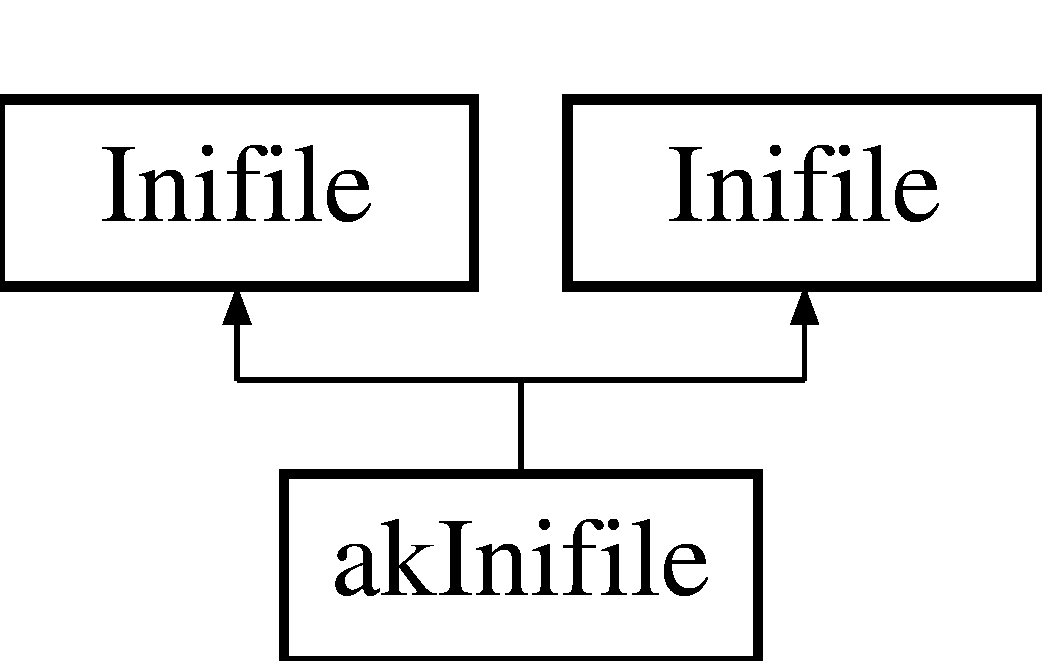
\includegraphics[height=2.000000cm]{classakInifile}
\end{center}
\end{figure}
\subsection*{Public Member Functions}
\begin{DoxyCompactItemize}
\item 
\hyperlink{classakInifile_a1e9d24ec7cccf0bc5897ec53fe71e9d9}{ak\-Inifile} (const char $\ast$filename, F\-I\-L\-E $\ast$\hyperlink{classakInifile_a9c55ea25efdedced0815835562454354}{logfile}=0, const char $\ast$second\-Dir=0, const char $\ast$third\-Dir=0)
\item 
\hyperlink{classakInifile_abf7f09a88016cafb4b7d3a7baa7f25f9}{$\sim$ak\-Inifile} ()
\item 
\hyperlink{classInifile_a42a1cfa6fc8618c8b28d449626f0ecde}{result} \hyperlink{classakInifile_a470c40676b92718698ecbb3055e2c2b1}{Specify\-Group} (const char $\ast$string)
\item 
int \hyperlink{classakInifile_ae17125c1f87eab81b1843f33cf68a949}{Get\-First\-Value} (const char $\ast$entry, int def\-Value, \hyperlink{classInifile_a42a1cfa6fc8618c8b28d449626f0ecde}{result} $\ast$error)
\item 
int \hyperlink{classakInifile_a8d14c6541da3f0ab9de6c788bbbabc42}{Get\-Next\-Value} (int def\-Value, \hyperlink{classInifile_a42a1cfa6fc8618c8b28d449626f0ecde}{result} $\ast$error)
\item 
char $\ast$ \hyperlink{classakInifile_a34c9714861ffe91f1a1e2a13c0b2a0c9}{Get\-First\-String} (const char $\ast$entry, const char $\ast$def\-String, \hyperlink{classInifile_a42a1cfa6fc8618c8b28d449626f0ecde}{result} $\ast$error)
\item 
char $\ast$ \hyperlink{classakInifile_a9dc548353a814f8e756c76eb6c960b8b}{Get\-Next\-String} (const char $\ast$def\-String, \hyperlink{classInifile_a42a1cfa6fc8618c8b28d449626f0ecde}{result} $\ast$error)
\item 
char $\ast$ \hyperlink{classakInifile_af67d760bc22ad6a48e1b1c9157d54dab}{Get\-Full\-String} (const char $\ast$entry, const char $\ast$def\-String, \hyperlink{classInifile_a42a1cfa6fc8618c8b28d449626f0ecde}{result} $\ast$error)
\item 
char $\ast$ \hyperlink{classakInifile_af2e11814e8311e9cf2d18b5afad7b7c8}{Get\-Full\-String} (const char $\ast$entry)
\item 
double \hyperlink{classakInifile_a84e553a71b399b79190a6d3215efac91}{Get\-First\-Value} (const char $\ast$entry, double def\-Value, \hyperlink{classInifile_a42a1cfa6fc8618c8b28d449626f0ecde}{result} $\ast$error)
\item 
double \hyperlink{classakInifile_a563076300ca6e4dd46850b27bc326aa6}{Get\-Next\-Value} (double def\-Value, \hyperlink{classInifile_a42a1cfa6fc8618c8b28d449626f0ecde}{result} $\ast$error)
\item 
double \hyperlink{classakInifile_a8121e22f645f39782132d198edc7ebd7}{Get\-First\-Double} (const char $\ast$entry, \hyperlink{classInifile_a42a1cfa6fc8618c8b28d449626f0ecde}{result} $\ast$error)
\item 
double \hyperlink{classakInifile_ad9c214f487ee936f5f8e83851a8e74e2}{Get\-Next\-Double} (\hyperlink{classInifile_a42a1cfa6fc8618c8b28d449626f0ecde}{result} $\ast$error)
\item 
void \hyperlink{classakInifile_a6832e33e59ce64f1a278d9abce9b9739}{set\-Debug\-Level} (int value)
\item 
\hyperlink{classakInifile_a1e9d24ec7cccf0bc5897ec53fe71e9d9}{ak\-Inifile} (const char $\ast$filename, F\-I\-L\-E $\ast$\hyperlink{classakInifile_a9c55ea25efdedced0815835562454354}{logfile}=0, const char $\ast$second\-Dir=0, const char $\ast$third\-Dir=0)
\item 
\hyperlink{classakInifile_abf7f09a88016cafb4b7d3a7baa7f25f9}{$\sim$ak\-Inifile} ()
\item 
\hyperlink{classInifile_a42a1cfa6fc8618c8b28d449626f0ecde}{result} \hyperlink{classakInifile_a39eba69b84b960c5ed456ee817f9e5c8}{Specify\-Group} (const char $\ast$string)
\item 
int \hyperlink{classakInifile_ae17125c1f87eab81b1843f33cf68a949}{Get\-First\-Value} (const char $\ast$entry, int def\-Value, \hyperlink{classInifile_a42a1cfa6fc8618c8b28d449626f0ecde}{result} $\ast$error)
\item 
int \hyperlink{classakInifile_a8d14c6541da3f0ab9de6c788bbbabc42}{Get\-Next\-Value} (int def\-Value, \hyperlink{classInifile_a42a1cfa6fc8618c8b28d449626f0ecde}{result} $\ast$error)
\item 
char $\ast$ \hyperlink{classakInifile_a90d845922ec84252ce460555cc984c10}{Get\-First\-String} (const char $\ast$entry, const char $\ast$def\-String, \hyperlink{classInifile_a42a1cfa6fc8618c8b28d449626f0ecde}{result} $\ast$error)
\item 
char $\ast$ \hyperlink{classakInifile_a5508037e2add9c20cf43dda40e8870d7}{Get\-Next\-String} (const char $\ast$def\-String, \hyperlink{classInifile_a42a1cfa6fc8618c8b28d449626f0ecde}{result} $\ast$error)
\item 
double \hyperlink{classakInifile_a84e553a71b399b79190a6d3215efac91}{Get\-First\-Value} (const char $\ast$entry, double def\-Value, \hyperlink{classInifile_a42a1cfa6fc8618c8b28d449626f0ecde}{result} $\ast$error)
\item 
double \hyperlink{classakInifile_a563076300ca6e4dd46850b27bc326aa6}{Get\-Next\-Value} (double def\-Value, \hyperlink{classInifile_a42a1cfa6fc8618c8b28d449626f0ecde}{result} $\ast$error)
\item 
double \hyperlink{classakInifile_a8121e22f645f39782132d198edc7ebd7}{Get\-First\-Double} (const char $\ast$entry, \hyperlink{classInifile_a42a1cfa6fc8618c8b28d449626f0ecde}{result} $\ast$error)
\item 
double \hyperlink{classakInifile_ad9c214f487ee936f5f8e83851a8e74e2}{Get\-Next\-Double} (\hyperlink{classInifile_a42a1cfa6fc8618c8b28d449626f0ecde}{result} $\ast$error)
\end{DoxyCompactItemize}
\subsection*{Protected Member Functions}
\begin{DoxyCompactItemize}
\item 
int \hyperlink{classakInifile_a9c1ec6087e2f42a2797d155738201e88}{open} (char $\ast$filename)
\item 
int \hyperlink{classakInifile_a91f29a8ed73a9d9d5172debad7519850}{concat\-Filename} (char $\ast$filepath, char $\ast$filename, char $\ast$dir)
\item 
int \hyperlink{classakInifile_a9c1ec6087e2f42a2797d155738201e88}{open} (char $\ast$filename)
\item 
int \hyperlink{classakInifile_a91f29a8ed73a9d9d5172debad7519850}{concat\-Filename} (char $\ast$filepath, char $\ast$filename, char $\ast$dir)
\end{DoxyCompactItemize}
\subsection*{Private Attributes}
\begin{DoxyCompactItemize}
\item 
F\-I\-L\-E $\ast$ \hyperlink{classakInifile_a9c55ea25efdedced0815835562454354}{logfile}
\item 
bool \hyperlink{classakInifile_aa1cb47c582ed7c93aae1a9ecfff6b0c2}{write\-Log}
\item 
int \hyperlink{classakInifile_a0b8a73d04d2b7a677bd61af9d87faec3}{debug}
\end{DoxyCompactItemize}
\subsection*{Additional Inherited Members}


\subsection{Detailed Description}
Extension of the inifile reader

New features\-: \begin{DoxyItemize}
\item Logging \item Default values\end{DoxyItemize}
Changes\-:
\begin{DoxyItemize}
\item 8.\-3.\-01 ak\-: Internal preprocessor define pragmas S\-U\-C\-C\-E\-S\-S and F\-A\-I\-L changed to k\-S\-U\-C\-C\-E\-S\-S and k\-F\-A\-I\-L 
\end{DoxyItemize}

\subsection{Constructor \& Destructor Documentation}
\hypertarget{classakInifile_a1e9d24ec7cccf0bc5897ec53fe71e9d9}{\index{ak\-Inifile@{ak\-Inifile}!ak\-Inifile@{ak\-Inifile}}
\index{ak\-Inifile@{ak\-Inifile}!akInifile@{ak\-Inifile}}
\subsubsection[{ak\-Inifile}]{\setlength{\rightskip}{0pt plus 5cm}ak\-Inifile\-::ak\-Inifile (
\begin{DoxyParamCaption}
\item[{const char $\ast$}]{filename, }
\item[{F\-I\-L\-E $\ast$}]{logfile = {\ttfamily 0}, }
\item[{const char $\ast$}]{second\-Dir = {\ttfamily 0}, }
\item[{const char $\ast$}]{third\-Dir = {\ttfamily 0}}
\end{DoxyParamCaption}
)}}\label{classakInifile_a1e9d24ec7cccf0bc5897ec53fe71e9d9}
\hypertarget{classakInifile_abf7f09a88016cafb4b7d3a7baa7f25f9}{\index{ak\-Inifile@{ak\-Inifile}!$\sim$ak\-Inifile@{$\sim$ak\-Inifile}}
\index{$\sim$ak\-Inifile@{$\sim$ak\-Inifile}!akInifile@{ak\-Inifile}}
\subsubsection[{$\sim$ak\-Inifile}]{\setlength{\rightskip}{0pt plus 5cm}ak\-Inifile\-::$\sim$ak\-Inifile (
\begin{DoxyParamCaption}
{}
\end{DoxyParamCaption}
)}}\label{classakInifile_abf7f09a88016cafb4b7d3a7baa7f25f9}
\hypertarget{classakInifile_a1e9d24ec7cccf0bc5897ec53fe71e9d9}{\index{ak\-Inifile@{ak\-Inifile}!ak\-Inifile@{ak\-Inifile}}
\index{ak\-Inifile@{ak\-Inifile}!akInifile@{ak\-Inifile}}
\subsubsection[{ak\-Inifile}]{\setlength{\rightskip}{0pt plus 5cm}ak\-Inifile\-::ak\-Inifile (
\begin{DoxyParamCaption}
\item[{const char $\ast$}]{filename, }
\item[{F\-I\-L\-E $\ast$}]{logfile = {\ttfamily 0}, }
\item[{const char $\ast$}]{second\-Dir = {\ttfamily 0}, }
\item[{const char $\ast$}]{third\-Dir = {\ttfamily 0}}
\end{DoxyParamCaption}
)}}\label{classakInifile_a1e9d24ec7cccf0bc5897ec53fe71e9d9}
\hypertarget{classakInifile_abf7f09a88016cafb4b7d3a7baa7f25f9}{\index{ak\-Inifile@{ak\-Inifile}!$\sim$ak\-Inifile@{$\sim$ak\-Inifile}}
\index{$\sim$ak\-Inifile@{$\sim$ak\-Inifile}!akInifile@{ak\-Inifile}}
\subsubsection[{$\sim$ak\-Inifile}]{\setlength{\rightskip}{0pt plus 5cm}ak\-Inifile\-::$\sim$ak\-Inifile (
\begin{DoxyParamCaption}
{}
\end{DoxyParamCaption}
)}}\label{classakInifile_abf7f09a88016cafb4b7d3a7baa7f25f9}


\subsection{Member Function Documentation}
\hypertarget{classakInifile_a91f29a8ed73a9d9d5172debad7519850}{\index{ak\-Inifile@{ak\-Inifile}!concat\-Filename@{concat\-Filename}}
\index{concat\-Filename@{concat\-Filename}!akInifile@{ak\-Inifile}}
\subsubsection[{concat\-Filename}]{\setlength{\rightskip}{0pt plus 5cm}int ak\-Inifile\-::concat\-Filename (
\begin{DoxyParamCaption}
\item[{char $\ast$}]{filepath, }
\item[{char $\ast$}]{filename, }
\item[{char $\ast$}]{dir}
\end{DoxyParamCaption}
)\hspace{0.3cm}{\ttfamily [protected]}}}\label{classakInifile_a91f29a8ed73a9d9d5172debad7519850}
Concat filename and directory to the filepath. The directory entry can also be a environment variable (e.\-g. \$\-H\-O\-M\-E) \hypertarget{classakInifile_a91f29a8ed73a9d9d5172debad7519850}{\index{ak\-Inifile@{ak\-Inifile}!concat\-Filename@{concat\-Filename}}
\index{concat\-Filename@{concat\-Filename}!akInifile@{ak\-Inifile}}
\subsubsection[{concat\-Filename}]{\setlength{\rightskip}{0pt plus 5cm}int ak\-Inifile\-::concat\-Filename (
\begin{DoxyParamCaption}
\item[{char $\ast$}]{filepath, }
\item[{char $\ast$}]{filename, }
\item[{char $\ast$}]{dir}
\end{DoxyParamCaption}
)\hspace{0.3cm}{\ttfamily [protected]}}}\label{classakInifile_a91f29a8ed73a9d9d5172debad7519850}
Concat filename and directory to the filepath. The directory entry can also be a environment variable (e.\-g. \$\-H\-O\-M\-E) \hypertarget{classakInifile_a8121e22f645f39782132d198edc7ebd7}{\index{ak\-Inifile@{ak\-Inifile}!Get\-First\-Double@{Get\-First\-Double}}
\index{Get\-First\-Double@{Get\-First\-Double}!akInifile@{ak\-Inifile}}
\subsubsection[{Get\-First\-Double}]{\setlength{\rightskip}{0pt plus 5cm}double ak\-Inifile\-::\-Get\-First\-Double (
\begin{DoxyParamCaption}
\item[{const char $\ast$}]{entry, }
\item[{{\bf result} $\ast$}]{error}
\end{DoxyParamCaption}
)}}\label{classakInifile_a8121e22f645f39782132d198edc7ebd7}
\hypertarget{classakInifile_a8121e22f645f39782132d198edc7ebd7}{\index{ak\-Inifile@{ak\-Inifile}!Get\-First\-Double@{Get\-First\-Double}}
\index{Get\-First\-Double@{Get\-First\-Double}!akInifile@{ak\-Inifile}}
\subsubsection[{Get\-First\-Double}]{\setlength{\rightskip}{0pt plus 5cm}double ak\-Inifile\-::\-Get\-First\-Double (
\begin{DoxyParamCaption}
\item[{const char $\ast$}]{entry, }
\item[{{\bf result} $\ast$}]{error}
\end{DoxyParamCaption}
)}}\label{classakInifile_a8121e22f645f39782132d198edc7ebd7}
\hypertarget{classakInifile_a90d845922ec84252ce460555cc984c10}{\index{ak\-Inifile@{ak\-Inifile}!Get\-First\-String@{Get\-First\-String}}
\index{Get\-First\-String@{Get\-First\-String}!akInifile@{ak\-Inifile}}
\subsubsection[{Get\-First\-String}]{\setlength{\rightskip}{0pt plus 5cm}char$\ast$ ak\-Inifile\-::\-Get\-First\-String (
\begin{DoxyParamCaption}
\item[{const char $\ast$}]{entry, }
\item[{const char $\ast$}]{def\-String, }
\item[{{\bf result} $\ast$}]{error}
\end{DoxyParamCaption}
)}}\label{classakInifile_a90d845922ec84252ce460555cc984c10}
\hypertarget{classakInifile_a34c9714861ffe91f1a1e2a13c0b2a0c9}{\index{ak\-Inifile@{ak\-Inifile}!Get\-First\-String@{Get\-First\-String}}
\index{Get\-First\-String@{Get\-First\-String}!akInifile@{ak\-Inifile}}
\subsubsection[{Get\-First\-String}]{\setlength{\rightskip}{0pt plus 5cm}char $\ast$ ak\-Inifile\-::\-Get\-First\-String (
\begin{DoxyParamCaption}
\item[{const char $\ast$}]{entry, }
\item[{const char $\ast$}]{def\-String, }
\item[{{\bf result} $\ast$}]{error}
\end{DoxyParamCaption}
)}}\label{classakInifile_a34c9714861ffe91f1a1e2a13c0b2a0c9}
\hypertarget{classakInifile_ae17125c1f87eab81b1843f33cf68a949}{\index{ak\-Inifile@{ak\-Inifile}!Get\-First\-Value@{Get\-First\-Value}}
\index{Get\-First\-Value@{Get\-First\-Value}!akInifile@{ak\-Inifile}}
\subsubsection[{Get\-First\-Value}]{\setlength{\rightskip}{0pt plus 5cm}int ak\-Inifile\-::\-Get\-First\-Value (
\begin{DoxyParamCaption}
\item[{const char $\ast$}]{entry, }
\item[{int}]{def\-Value, }
\item[{{\bf result} $\ast$}]{error}
\end{DoxyParamCaption}
)}}\label{classakInifile_ae17125c1f87eab81b1843f33cf68a949}
\hypertarget{classakInifile_ae17125c1f87eab81b1843f33cf68a949}{\index{ak\-Inifile@{ak\-Inifile}!Get\-First\-Value@{Get\-First\-Value}}
\index{Get\-First\-Value@{Get\-First\-Value}!akInifile@{ak\-Inifile}}
\subsubsection[{Get\-First\-Value}]{\setlength{\rightskip}{0pt plus 5cm}int ak\-Inifile\-::\-Get\-First\-Value (
\begin{DoxyParamCaption}
\item[{const char $\ast$}]{entry, }
\item[{int}]{def\-Value, }
\item[{{\bf result} $\ast$}]{error}
\end{DoxyParamCaption}
)}}\label{classakInifile_ae17125c1f87eab81b1843f33cf68a949}
\hypertarget{classakInifile_a84e553a71b399b79190a6d3215efac91}{\index{ak\-Inifile@{ak\-Inifile}!Get\-First\-Value@{Get\-First\-Value}}
\index{Get\-First\-Value@{Get\-First\-Value}!akInifile@{ak\-Inifile}}
\subsubsection[{Get\-First\-Value}]{\setlength{\rightskip}{0pt plus 5cm}double ak\-Inifile\-::\-Get\-First\-Value (
\begin{DoxyParamCaption}
\item[{const char $\ast$}]{entry, }
\item[{double}]{def\-Value, }
\item[{{\bf result} $\ast$}]{error}
\end{DoxyParamCaption}
)}}\label{classakInifile_a84e553a71b399b79190a6d3215efac91}
\hypertarget{classakInifile_a84e553a71b399b79190a6d3215efac91}{\index{ak\-Inifile@{ak\-Inifile}!Get\-First\-Value@{Get\-First\-Value}}
\index{Get\-First\-Value@{Get\-First\-Value}!akInifile@{ak\-Inifile}}
\subsubsection[{Get\-First\-Value}]{\setlength{\rightskip}{0pt plus 5cm}double ak\-Inifile\-::\-Get\-First\-Value (
\begin{DoxyParamCaption}
\item[{const char $\ast$}]{entry, }
\item[{double}]{def\-Value, }
\item[{{\bf result} $\ast$}]{error}
\end{DoxyParamCaption}
)}}\label{classakInifile_a84e553a71b399b79190a6d3215efac91}
\hypertarget{classakInifile_af67d760bc22ad6a48e1b1c9157d54dab}{\index{ak\-Inifile@{ak\-Inifile}!Get\-Full\-String@{Get\-Full\-String}}
\index{Get\-Full\-String@{Get\-Full\-String}!akInifile@{ak\-Inifile}}
\subsubsection[{Get\-Full\-String}]{\setlength{\rightskip}{0pt plus 5cm}char $\ast$ ak\-Inifile\-::\-Get\-Full\-String (
\begin{DoxyParamCaption}
\item[{const char $\ast$}]{entry, }
\item[{const char $\ast$}]{def\-String, }
\item[{{\bf result} $\ast$}]{error}
\end{DoxyParamCaption}
)}}\label{classakInifile_af67d760bc22ad6a48e1b1c9157d54dab}
Read the full string in a line. \hypertarget{classakInifile_af2e11814e8311e9cf2d18b5afad7b7c8}{\index{ak\-Inifile@{ak\-Inifile}!Get\-Full\-String@{Get\-Full\-String}}
\index{Get\-Full\-String@{Get\-Full\-String}!akInifile@{ak\-Inifile}}
\subsubsection[{Get\-Full\-String}]{\setlength{\rightskip}{0pt plus 5cm}char $\ast$ ak\-Inifile\-::\-Get\-Full\-String (
\begin{DoxyParamCaption}
\item[{const char $\ast$}]{entry}
\end{DoxyParamCaption}
)}}\label{classakInifile_af2e11814e8311e9cf2d18b5afad7b7c8}
\hypertarget{classakInifile_ad9c214f487ee936f5f8e83851a8e74e2}{\index{ak\-Inifile@{ak\-Inifile}!Get\-Next\-Double@{Get\-Next\-Double}}
\index{Get\-Next\-Double@{Get\-Next\-Double}!akInifile@{ak\-Inifile}}
\subsubsection[{Get\-Next\-Double}]{\setlength{\rightskip}{0pt plus 5cm}double ak\-Inifile\-::\-Get\-Next\-Double (
\begin{DoxyParamCaption}
\item[{{\bf result} $\ast$}]{error}
\end{DoxyParamCaption}
)}}\label{classakInifile_ad9c214f487ee936f5f8e83851a8e74e2}
\hypertarget{classakInifile_ad9c214f487ee936f5f8e83851a8e74e2}{\index{ak\-Inifile@{ak\-Inifile}!Get\-Next\-Double@{Get\-Next\-Double}}
\index{Get\-Next\-Double@{Get\-Next\-Double}!akInifile@{ak\-Inifile}}
\subsubsection[{Get\-Next\-Double}]{\setlength{\rightskip}{0pt plus 5cm}double ak\-Inifile\-::\-Get\-Next\-Double (
\begin{DoxyParamCaption}
\item[{{\bf result} $\ast$}]{error}
\end{DoxyParamCaption}
)}}\label{classakInifile_ad9c214f487ee936f5f8e83851a8e74e2}
\hypertarget{classakInifile_a5508037e2add9c20cf43dda40e8870d7}{\index{ak\-Inifile@{ak\-Inifile}!Get\-Next\-String@{Get\-Next\-String}}
\index{Get\-Next\-String@{Get\-Next\-String}!akInifile@{ak\-Inifile}}
\subsubsection[{Get\-Next\-String}]{\setlength{\rightskip}{0pt plus 5cm}char$\ast$ ak\-Inifile\-::\-Get\-Next\-String (
\begin{DoxyParamCaption}
\item[{const char $\ast$}]{def\-String, }
\item[{{\bf result} $\ast$}]{error}
\end{DoxyParamCaption}
)}}\label{classakInifile_a5508037e2add9c20cf43dda40e8870d7}
\hypertarget{classakInifile_a9dc548353a814f8e756c76eb6c960b8b}{\index{ak\-Inifile@{ak\-Inifile}!Get\-Next\-String@{Get\-Next\-String}}
\index{Get\-Next\-String@{Get\-Next\-String}!akInifile@{ak\-Inifile}}
\subsubsection[{Get\-Next\-String}]{\setlength{\rightskip}{0pt plus 5cm}char $\ast$ ak\-Inifile\-::\-Get\-Next\-String (
\begin{DoxyParamCaption}
\item[{const char $\ast$}]{def\-String, }
\item[{{\bf result} $\ast$}]{error}
\end{DoxyParamCaption}
)}}\label{classakInifile_a9dc548353a814f8e756c76eb6c960b8b}
\hypertarget{classakInifile_a8d14c6541da3f0ab9de6c788bbbabc42}{\index{ak\-Inifile@{ak\-Inifile}!Get\-Next\-Value@{Get\-Next\-Value}}
\index{Get\-Next\-Value@{Get\-Next\-Value}!akInifile@{ak\-Inifile}}
\subsubsection[{Get\-Next\-Value}]{\setlength{\rightskip}{0pt plus 5cm}int ak\-Inifile\-::\-Get\-Next\-Value (
\begin{DoxyParamCaption}
\item[{int}]{def\-Value, }
\item[{{\bf result} $\ast$}]{error}
\end{DoxyParamCaption}
)}}\label{classakInifile_a8d14c6541da3f0ab9de6c788bbbabc42}
\hypertarget{classakInifile_a8d14c6541da3f0ab9de6c788bbbabc42}{\index{ak\-Inifile@{ak\-Inifile}!Get\-Next\-Value@{Get\-Next\-Value}}
\index{Get\-Next\-Value@{Get\-Next\-Value}!akInifile@{ak\-Inifile}}
\subsubsection[{Get\-Next\-Value}]{\setlength{\rightskip}{0pt plus 5cm}int ak\-Inifile\-::\-Get\-Next\-Value (
\begin{DoxyParamCaption}
\item[{int}]{def\-Value, }
\item[{{\bf result} $\ast$}]{error}
\end{DoxyParamCaption}
)}}\label{classakInifile_a8d14c6541da3f0ab9de6c788bbbabc42}
\hypertarget{classakInifile_a563076300ca6e4dd46850b27bc326aa6}{\index{ak\-Inifile@{ak\-Inifile}!Get\-Next\-Value@{Get\-Next\-Value}}
\index{Get\-Next\-Value@{Get\-Next\-Value}!akInifile@{ak\-Inifile}}
\subsubsection[{Get\-Next\-Value}]{\setlength{\rightskip}{0pt plus 5cm}double ak\-Inifile\-::\-Get\-Next\-Value (
\begin{DoxyParamCaption}
\item[{double}]{def\-Value, }
\item[{{\bf result} $\ast$}]{error}
\end{DoxyParamCaption}
)}}\label{classakInifile_a563076300ca6e4dd46850b27bc326aa6}
\hypertarget{classakInifile_a563076300ca6e4dd46850b27bc326aa6}{\index{ak\-Inifile@{ak\-Inifile}!Get\-Next\-Value@{Get\-Next\-Value}}
\index{Get\-Next\-Value@{Get\-Next\-Value}!akInifile@{ak\-Inifile}}
\subsubsection[{Get\-Next\-Value}]{\setlength{\rightskip}{0pt plus 5cm}double ak\-Inifile\-::\-Get\-Next\-Value (
\begin{DoxyParamCaption}
\item[{double}]{def\-Value, }
\item[{{\bf result} $\ast$}]{error}
\end{DoxyParamCaption}
)}}\label{classakInifile_a563076300ca6e4dd46850b27bc326aa6}
\hypertarget{classakInifile_a9c1ec6087e2f42a2797d155738201e88}{\index{ak\-Inifile@{ak\-Inifile}!open@{open}}
\index{open@{open}!akInifile@{ak\-Inifile}}
\subsubsection[{open}]{\setlength{\rightskip}{0pt plus 5cm}int ak\-Inifile\-::open (
\begin{DoxyParamCaption}
\item[{char $\ast$}]{filename}
\end{DoxyParamCaption}
)\hspace{0.3cm}{\ttfamily [protected]}}}\label{classakInifile_a9c1ec6087e2f42a2797d155738201e88}
Try to open another file \hypertarget{classakInifile_a9c1ec6087e2f42a2797d155738201e88}{\index{ak\-Inifile@{ak\-Inifile}!open@{open}}
\index{open@{open}!akInifile@{ak\-Inifile}}
\subsubsection[{open}]{\setlength{\rightskip}{0pt plus 5cm}int ak\-Inifile\-::open (
\begin{DoxyParamCaption}
\item[{char $\ast$}]{filename}
\end{DoxyParamCaption}
)\hspace{0.3cm}{\ttfamily [protected]}}}\label{classakInifile_a9c1ec6087e2f42a2797d155738201e88}
Try to open another file \hypertarget{classakInifile_a6832e33e59ce64f1a278d9abce9b9739}{\index{ak\-Inifile@{ak\-Inifile}!set\-Debug\-Level@{set\-Debug\-Level}}
\index{set\-Debug\-Level@{set\-Debug\-Level}!akInifile@{ak\-Inifile}}
\subsubsection[{set\-Debug\-Level}]{\setlength{\rightskip}{0pt plus 5cm}void ak\-Inifile\-::set\-Debug\-Level (
\begin{DoxyParamCaption}
\item[{int}]{value}
\end{DoxyParamCaption}
)}}\label{classakInifile_a6832e33e59ce64f1a278d9abce9b9739}
Set the debug level -\/ 0 means no debug output \hypertarget{classakInifile_a39eba69b84b960c5ed456ee817f9e5c8}{\index{ak\-Inifile@{ak\-Inifile}!Specify\-Group@{Specify\-Group}}
\index{Specify\-Group@{Specify\-Group}!akInifile@{ak\-Inifile}}
\subsubsection[{Specify\-Group}]{\setlength{\rightskip}{0pt plus 5cm}{\bf result} ak\-Inifile\-::\-Specify\-Group (
\begin{DoxyParamCaption}
\item[{const char $\ast$}]{string}
\end{DoxyParamCaption}
)}}\label{classakInifile_a39eba69b84b960c5ed456ee817f9e5c8}
\hypertarget{classakInifile_a470c40676b92718698ecbb3055e2c2b1}{\index{ak\-Inifile@{ak\-Inifile}!Specify\-Group@{Specify\-Group}}
\index{Specify\-Group@{Specify\-Group}!akInifile@{ak\-Inifile}}
\subsubsection[{Specify\-Group}]{\setlength{\rightskip}{0pt plus 5cm}{\bf Inifile\-::result} ak\-Inifile\-::\-Specify\-Group (
\begin{DoxyParamCaption}
\item[{const char $\ast$}]{string}
\end{DoxyParamCaption}
)}}\label{classakInifile_a470c40676b92718698ecbb3055e2c2b1}


\subsection{Member Data Documentation}
\hypertarget{classakInifile_a0b8a73d04d2b7a677bd61af9d87faec3}{\index{ak\-Inifile@{ak\-Inifile}!debug@{debug}}
\index{debug@{debug}!akInifile@{ak\-Inifile}}
\subsubsection[{debug}]{\setlength{\rightskip}{0pt plus 5cm}int ak\-Inifile\-::debug\hspace{0.3cm}{\ttfamily [private]}}}\label{classakInifile_a0b8a73d04d2b7a677bd61af9d87faec3}
Debug level \hypertarget{classakInifile_a9c55ea25efdedced0815835562454354}{\index{ak\-Inifile@{ak\-Inifile}!logfile@{logfile}}
\index{logfile@{logfile}!akInifile@{ak\-Inifile}}
\subsubsection[{logfile}]{\setlength{\rightskip}{0pt plus 5cm}F\-I\-L\-E $\ast$ ak\-Inifile\-::logfile\hspace{0.3cm}{\ttfamily [private]}}}\label{classakInifile_a9c55ea25efdedced0815835562454354}
\hypertarget{classakInifile_aa1cb47c582ed7c93aae1a9ecfff6b0c2}{\index{ak\-Inifile@{ak\-Inifile}!write\-Log@{write\-Log}}
\index{write\-Log@{write\-Log}!akInifile@{ak\-Inifile}}
\subsubsection[{write\-Log}]{\setlength{\rightskip}{0pt plus 5cm}bool ak\-Inifile\-::write\-Log\hspace{0.3cm}{\ttfamily [private]}}}\label{classakInifile_aa1cb47c582ed7c93aae1a9ecfff6b0c2}
Flag set if logging output is required 

The documentation for this class was generated from the following files\-:\begin{DoxyCompactItemize}
\item 
/home/ntj/\-Development/phd/kitcube-\/tools/src/akutil/\hyperlink{akinifile_8h}{akinifile.\-h}\item 
/home/ntj/\-Development/phd/kitcube-\/tools/src/akutil.\-minimal/\hyperlink{minimal_2akinifile_8h}{akinifile.\-h}\item 
/home/ntj/\-Development/phd/kitcube-\/tools/src/akutil/\hyperlink{akinifile_8cpp}{akinifile.\-cpp}\item 
/home/ntj/\-Development/phd/kitcube-\/tools/src/akutil.\-minimal/\hyperlink{minimal_2akinifile_8cpp}{akinifile.\-cpp}\end{DoxyCompactItemize}

\hypertarget{classakSingleton}{\section{ak\-Singleton Class Reference}
\label{classakSingleton}\index{ak\-Singleton@{ak\-Singleton}}
}


{\ttfamily \#include $<$aksingleton.\-h$>$}

Inheritance diagram for ak\-Singleton\-:\begin{figure}[H]
\begin{center}
\leavevmode
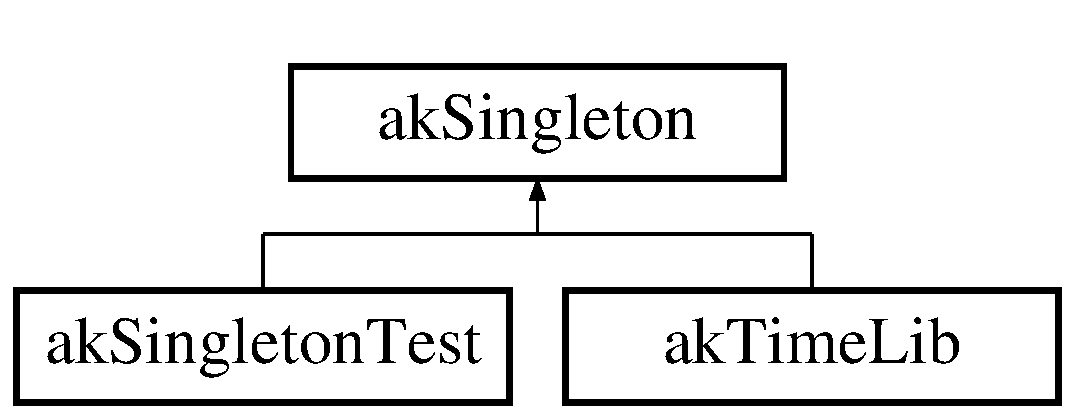
\includegraphics[height=2.000000cm]{classakSingleton}
\end{center}
\end{figure}
\subsection*{Public Member Functions}
\begin{DoxyCompactItemize}
\item 
\hyperlink{classakSingleton_aa68086f723700b6b16304b9fe3a8fd29}{ak\-Singleton} ()
\item 
\hyperlink{classakSingleton_a285373122987a0dae45fe3d538f37320}{$\sim$ak\-Singleton} ()
\end{DoxyCompactItemize}


\subsection{Detailed Description}
A singleton base class used by \hyperlink{classakSingletonCleaner}{ak\-Singleton\-Cleaner} 

\subsection{Constructor \& Destructor Documentation}
\hypertarget{classakSingleton_aa68086f723700b6b16304b9fe3a8fd29}{\index{ak\-Singleton@{ak\-Singleton}!ak\-Singleton@{ak\-Singleton}}
\index{ak\-Singleton@{ak\-Singleton}!akSingleton@{ak\-Singleton}}
\subsubsection[{ak\-Singleton}]{\setlength{\rightskip}{0pt plus 5cm}ak\-Singleton\-::ak\-Singleton (
\begin{DoxyParamCaption}
{}
\end{DoxyParamCaption}
)}}\label{classakSingleton_aa68086f723700b6b16304b9fe3a8fd29}
\hypertarget{classakSingleton_a285373122987a0dae45fe3d538f37320}{\index{ak\-Singleton@{ak\-Singleton}!$\sim$ak\-Singleton@{$\sim$ak\-Singleton}}
\index{$\sim$ak\-Singleton@{$\sim$ak\-Singleton}!akSingleton@{ak\-Singleton}}
\subsubsection[{$\sim$ak\-Singleton}]{\setlength{\rightskip}{0pt plus 5cm}ak\-Singleton\-::$\sim$ak\-Singleton (
\begin{DoxyParamCaption}
{}
\end{DoxyParamCaption}
)}}\label{classakSingleton_a285373122987a0dae45fe3d538f37320}


The documentation for this class was generated from the following files\-:\begin{DoxyCompactItemize}
\item 
/home/ntj/\-Development/phd/kitcube-\/tools/src/akutil/\hyperlink{aksingleton_8h}{aksingleton.\-h}\item 
/home/ntj/\-Development/phd/kitcube-\/tools/src/akutil/\hyperlink{aksingleton_8cpp}{aksingleton.\-cpp}\end{DoxyCompactItemize}

\hypertarget{classakSingletonCleaner}{\section{ak\-Singleton\-Cleaner Class Reference}
\label{classakSingletonCleaner}\index{ak\-Singleton\-Cleaner@{ak\-Singleton\-Cleaner}}
}


{\ttfamily \#include $<$aksingletoncleaner.\-h$>$}

\subsection*{Public Member Functions}
\begin{DoxyCompactItemize}
\item 
\hyperlink{classakSingletonCleaner_a32e58e12cf09e734bc193cc173109a11}{ak\-Singleton\-Cleaner} (\hyperlink{classakSingleton}{ak\-Singleton} $\ast$p\-Object=0)
\item 
virtual \hyperlink{classakSingletonCleaner_ac67a209ea9bcfa84b7023d0b883f2760}{$\sim$ak\-Singleton\-Cleaner} ()
\item 
void \hyperlink{classakSingletonCleaner_aec9467ff1fe3a122cdb0b2804de534f1}{set\-Object} (\hyperlink{classakSingleton}{ak\-Singleton} $\ast$p\-Object)
\item 
void \hyperlink{classakSingletonCleaner_a71f6982f436425a3ffd863831014241a}{dump} ()
\item 
\hyperlink{classakSingleton}{ak\-Singleton} $\ast$ \hyperlink{classakSingletonCleaner_ade327d63224d0a197643234112298313}{get\-Object} ()
\end{DoxyCompactItemize}
\subsection*{Private Attributes}
\begin{DoxyCompactItemize}
\item 
\hyperlink{classakSingleton}{ak\-Singleton} $\ast$ \hyperlink{classakSingletonCleaner_aae2ff315a00eb9214a6212e50feaab97}{singleton}
\end{DoxyCompactItemize}


\subsection{Detailed Description}
Avoid memory leakage through instances of singletons. 

\subsection{Constructor \& Destructor Documentation}
\hypertarget{classakSingletonCleaner_a32e58e12cf09e734bc193cc173109a11}{\index{ak\-Singleton\-Cleaner@{ak\-Singleton\-Cleaner}!ak\-Singleton\-Cleaner@{ak\-Singleton\-Cleaner}}
\index{ak\-Singleton\-Cleaner@{ak\-Singleton\-Cleaner}!akSingletonCleaner@{ak\-Singleton\-Cleaner}}
\subsubsection[{ak\-Singleton\-Cleaner}]{\setlength{\rightskip}{0pt plus 5cm}ak\-Singleton\-Cleaner\-::ak\-Singleton\-Cleaner (
\begin{DoxyParamCaption}
\item[{{\bf ak\-Singleton} $\ast$}]{p\-Object = {\ttfamily 0}}
\end{DoxyParamCaption}
)\hspace{0.3cm}{\ttfamily [inline]}}}\label{classakSingletonCleaner_a32e58e12cf09e734bc193cc173109a11}
Constructor \hypertarget{classakSingletonCleaner_ac67a209ea9bcfa84b7023d0b883f2760}{\index{ak\-Singleton\-Cleaner@{ak\-Singleton\-Cleaner}!$\sim$ak\-Singleton\-Cleaner@{$\sim$ak\-Singleton\-Cleaner}}
\index{$\sim$ak\-Singleton\-Cleaner@{$\sim$ak\-Singleton\-Cleaner}!akSingletonCleaner@{ak\-Singleton\-Cleaner}}
\subsubsection[{$\sim$ak\-Singleton\-Cleaner}]{\setlength{\rightskip}{0pt plus 5cm}virtual ak\-Singleton\-Cleaner\-::$\sim$ak\-Singleton\-Cleaner (
\begin{DoxyParamCaption}
{}
\end{DoxyParamCaption}
)\hspace{0.3cm}{\ttfamily [inline]}, {\ttfamily [virtual]}}}\label{classakSingletonCleaner_ac67a209ea9bcfa84b7023d0b883f2760}
Static objects will be deleted at the program end. So every singleton class needs to contain a static oject of type \hyperlink{classakSingletonCleaner}{ak\-Singleton\-Cleaner} and pass it own reference to this object 

\subsection{Member Function Documentation}
\hypertarget{classakSingletonCleaner_a71f6982f436425a3ffd863831014241a}{\index{ak\-Singleton\-Cleaner@{ak\-Singleton\-Cleaner}!dump@{dump}}
\index{dump@{dump}!akSingletonCleaner@{ak\-Singleton\-Cleaner}}
\subsubsection[{dump}]{\setlength{\rightskip}{0pt plus 5cm}void ak\-Singleton\-Cleaner\-::dump (
\begin{DoxyParamCaption}
{}
\end{DoxyParamCaption}
)\hspace{0.3cm}{\ttfamily [inline]}}}\label{classakSingletonCleaner_a71f6982f436425a3ffd863831014241a}
\hypertarget{classakSingletonCleaner_ade327d63224d0a197643234112298313}{\index{ak\-Singleton\-Cleaner@{ak\-Singleton\-Cleaner}!get\-Object@{get\-Object}}
\index{get\-Object@{get\-Object}!akSingletonCleaner@{ak\-Singleton\-Cleaner}}
\subsubsection[{get\-Object}]{\setlength{\rightskip}{0pt plus 5cm}{\bf ak\-Singleton}$\ast$ ak\-Singleton\-Cleaner\-::get\-Object (
\begin{DoxyParamCaption}
{}
\end{DoxyParamCaption}
)\hspace{0.3cm}{\ttfamily [inline]}}}\label{classakSingletonCleaner_ade327d63224d0a197643234112298313}
\hypertarget{classakSingletonCleaner_aec9467ff1fe3a122cdb0b2804de534f1}{\index{ak\-Singleton\-Cleaner@{ak\-Singleton\-Cleaner}!set\-Object@{set\-Object}}
\index{set\-Object@{set\-Object}!akSingletonCleaner@{ak\-Singleton\-Cleaner}}
\subsubsection[{set\-Object}]{\setlength{\rightskip}{0pt plus 5cm}void ak\-Singleton\-Cleaner\-::set\-Object (
\begin{DoxyParamCaption}
\item[{{\bf ak\-Singleton} $\ast$}]{p\-Object}
\end{DoxyParamCaption}
)\hspace{0.3cm}{\ttfamily [inline]}}}\label{classakSingletonCleaner_aec9467ff1fe3a122cdb0b2804de534f1}


\subsection{Member Data Documentation}
\hypertarget{classakSingletonCleaner_aae2ff315a00eb9214a6212e50feaab97}{\index{ak\-Singleton\-Cleaner@{ak\-Singleton\-Cleaner}!singleton@{singleton}}
\index{singleton@{singleton}!akSingletonCleaner@{ak\-Singleton\-Cleaner}}
\subsubsection[{singleton}]{\setlength{\rightskip}{0pt plus 5cm}{\bf ak\-Singleton}$\ast$ ak\-Singleton\-Cleaner\-::singleton\hspace{0.3cm}{\ttfamily [private]}}}\label{classakSingletonCleaner_aae2ff315a00eb9214a6212e50feaab97}
Reference of the singleton to care for 

The documentation for this class was generated from the following file\-:\begin{DoxyCompactItemize}
\item 
/home/ntj/\-Development/phd/kitcube-\/tools/src/akutil/\hyperlink{aksingletoncleaner_8h}{aksingletoncleaner.\-h}\end{DoxyCompactItemize}

\hypertarget{classakSingletonTest}{\section{ak\-Singleton\-Test Class Reference}
\label{classakSingletonTest}\index{ak\-Singleton\-Test@{ak\-Singleton\-Test}}
}


{\ttfamily \#include $<$aksingletontest.\-h$>$}

Inheritance diagram for ak\-Singleton\-Test\-:\begin{figure}[H]
\begin{center}
\leavevmode
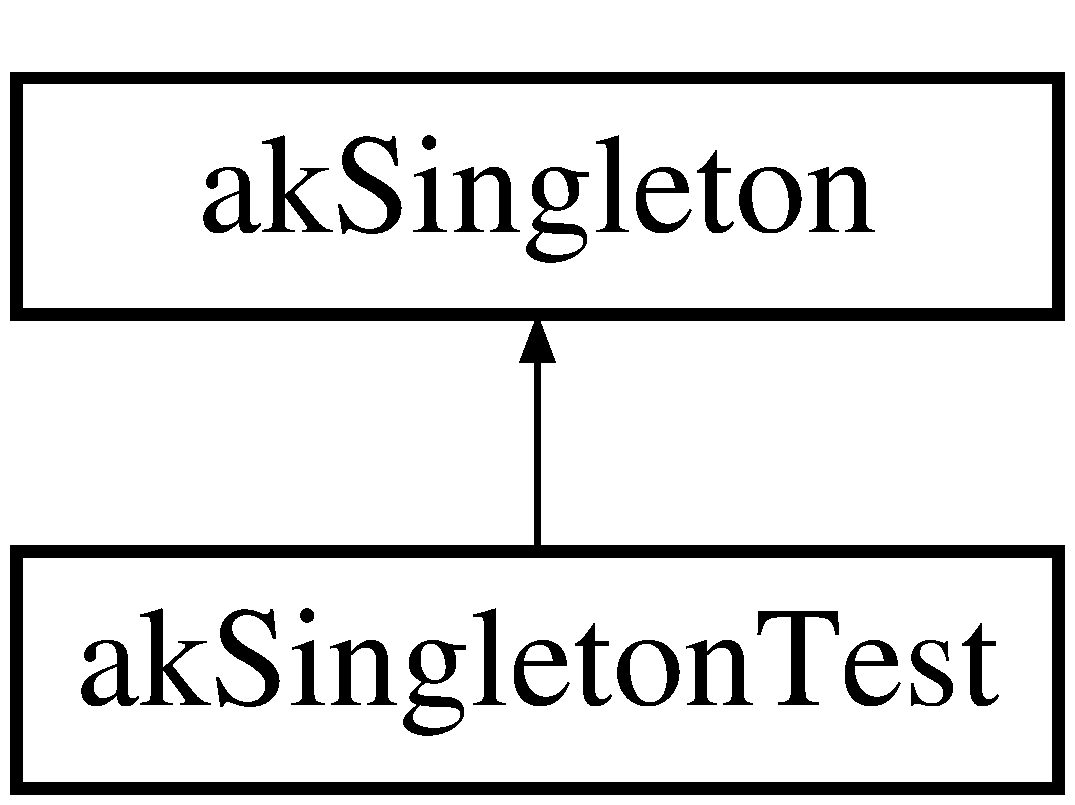
\includegraphics[height=2.000000cm]{classakSingletonTest}
\end{center}
\end{figure}
\subsection*{Public Member Functions}
\begin{DoxyCompactItemize}
\item 
\hyperlink{classakSingletonTest_a82107dda3518b31bb4e28333735f2e7d}{$\sim$ak\-Singleton\-Test} ()
\item 
void \hyperlink{classakSingletonTest_af45b897fec455882164f13b8865a3b3e}{dump} ()
\end{DoxyCompactItemize}
\subsection*{Static Public Member Functions}
\begin{DoxyCompactItemize}
\item 
static \hyperlink{classakSingletonTest}{ak\-Singleton\-Test} $\ast$ \hyperlink{classakSingletonTest_a0dde72606efb09c8d53a2dfd2aeaa79c}{get\-Reference} ()
\end{DoxyCompactItemize}
\subsection*{Protected Member Functions}
\begin{DoxyCompactItemize}
\item 
\hyperlink{classakSingletonTest_a8b16413a830e70b3dd6c4ecc7d14449f}{ak\-Singleton\-Test} ()
\end{DoxyCompactItemize}
\subsection*{Static Private Attributes}
\begin{DoxyCompactItemize}
\item 
static \hyperlink{classakSingletonTest}{ak\-Singleton\-Test} \hyperlink{classakSingletonTest_a08427ba4539841d113a7fd663e554928}{instance}
\item 
static \hyperlink{classakSingletonCleaner}{ak\-Singleton\-Cleaner} \hyperlink{classakSingletonTest_a3662e8962e2e70a23a5be1d050c2b4f7}{cleaner}
\end{DoxyCompactItemize}


\subsection{Detailed Description}
A test singleton! 

\subsection{Constructor \& Destructor Documentation}
\hypertarget{classakSingletonTest_a8b16413a830e70b3dd6c4ecc7d14449f}{\index{ak\-Singleton\-Test@{ak\-Singleton\-Test}!ak\-Singleton\-Test@{ak\-Singleton\-Test}}
\index{ak\-Singleton\-Test@{ak\-Singleton\-Test}!akSingletonTest@{ak\-Singleton\-Test}}
\subsubsection[{ak\-Singleton\-Test}]{\setlength{\rightskip}{0pt plus 5cm}ak\-Singleton\-Test\-::ak\-Singleton\-Test (
\begin{DoxyParamCaption}
{}
\end{DoxyParamCaption}
)\hspace{0.3cm}{\ttfamily [protected]}}}\label{classakSingletonTest_a8b16413a830e70b3dd6c4ecc7d14449f}
\hypertarget{classakSingletonTest_a82107dda3518b31bb4e28333735f2e7d}{\index{ak\-Singleton\-Test@{ak\-Singleton\-Test}!$\sim$ak\-Singleton\-Test@{$\sim$ak\-Singleton\-Test}}
\index{$\sim$ak\-Singleton\-Test@{$\sim$ak\-Singleton\-Test}!akSingletonTest@{ak\-Singleton\-Test}}
\subsubsection[{$\sim$ak\-Singleton\-Test}]{\setlength{\rightskip}{0pt plus 5cm}ak\-Singleton\-Test\-::$\sim$ak\-Singleton\-Test (
\begin{DoxyParamCaption}
{}
\end{DoxyParamCaption}
)\hspace{0.3cm}{\ttfamily [inline]}}}\label{classakSingletonTest_a82107dda3518b31bb4e28333735f2e7d}


\subsection{Member Function Documentation}
\hypertarget{classakSingletonTest_af45b897fec455882164f13b8865a3b3e}{\index{ak\-Singleton\-Test@{ak\-Singleton\-Test}!dump@{dump}}
\index{dump@{dump}!akSingletonTest@{ak\-Singleton\-Test}}
\subsubsection[{dump}]{\setlength{\rightskip}{0pt plus 5cm}void ak\-Singleton\-Test\-::dump (
\begin{DoxyParamCaption}
{}
\end{DoxyParamCaption}
)\hspace{0.3cm}{\ttfamily [inline]}}}\label{classakSingletonTest_af45b897fec455882164f13b8865a3b3e}
\hypertarget{classakSingletonTest_a0dde72606efb09c8d53a2dfd2aeaa79c}{\index{ak\-Singleton\-Test@{ak\-Singleton\-Test}!get\-Reference@{get\-Reference}}
\index{get\-Reference@{get\-Reference}!akSingletonTest@{ak\-Singleton\-Test}}
\subsubsection[{get\-Reference}]{\setlength{\rightskip}{0pt plus 5cm}{\bf ak\-Singleton\-Test} $\ast$ ak\-Singleton\-Test\-::get\-Reference (
\begin{DoxyParamCaption}
{}
\end{DoxyParamCaption}
)\hspace{0.3cm}{\ttfamily [static]}}}\label{classakSingletonTest_a0dde72606efb09c8d53a2dfd2aeaa79c}


\subsection{Member Data Documentation}
\hypertarget{classakSingletonTest_a3662e8962e2e70a23a5be1d050c2b4f7}{\index{ak\-Singleton\-Test@{ak\-Singleton\-Test}!cleaner@{cleaner}}
\index{cleaner@{cleaner}!akSingletonTest@{ak\-Singleton\-Test}}
\subsubsection[{cleaner}]{\setlength{\rightskip}{0pt plus 5cm}{\bf ak\-Singleton\-Cleaner} ak\-Singleton\-Test\-::cleaner\hspace{0.3cm}{\ttfamily [static]}, {\ttfamily [private]}}}\label{classakSingletonTest_a3662e8962e2e70a23a5be1d050c2b4f7}
Attention\-: cleaner has to be defined before instance !!! \hypertarget{classakSingletonTest_a08427ba4539841d113a7fd663e554928}{\index{ak\-Singleton\-Test@{ak\-Singleton\-Test}!instance@{instance}}
\index{instance@{instance}!akSingletonTest@{ak\-Singleton\-Test}}
\subsubsection[{instance}]{\setlength{\rightskip}{0pt plus 5cm}{\bf ak\-Singleton\-Test} ak\-Singleton\-Test\-::instance\hspace{0.3cm}{\ttfamily [static]}, {\ttfamily [private]}}}\label{classakSingletonTest_a08427ba4539841d113a7fd663e554928}


The documentation for this class was generated from the following files\-:\begin{DoxyCompactItemize}
\item 
/home/ntj/\-Development/phd/kitcube-\/tools/src/akutil/\hyperlink{aksingletontest_8h}{aksingletontest.\-h}\item 
/home/ntj/\-Development/phd/kitcube-\/tools/src/akutil/\hyperlink{aksingletontest_8cpp}{aksingletontest.\-cpp}\end{DoxyCompactItemize}

\hypertarget{classakTimeLib}{\section{ak\-Time\-Lib Class Reference}
\label{classakTimeLib}\index{ak\-Time\-Lib@{ak\-Time\-Lib}}
}


{\ttfamily \#include $<$aktimelib.\-h$>$}

Inheritance diagram for ak\-Time\-Lib\-:\begin{figure}[H]
\begin{center}
\leavevmode
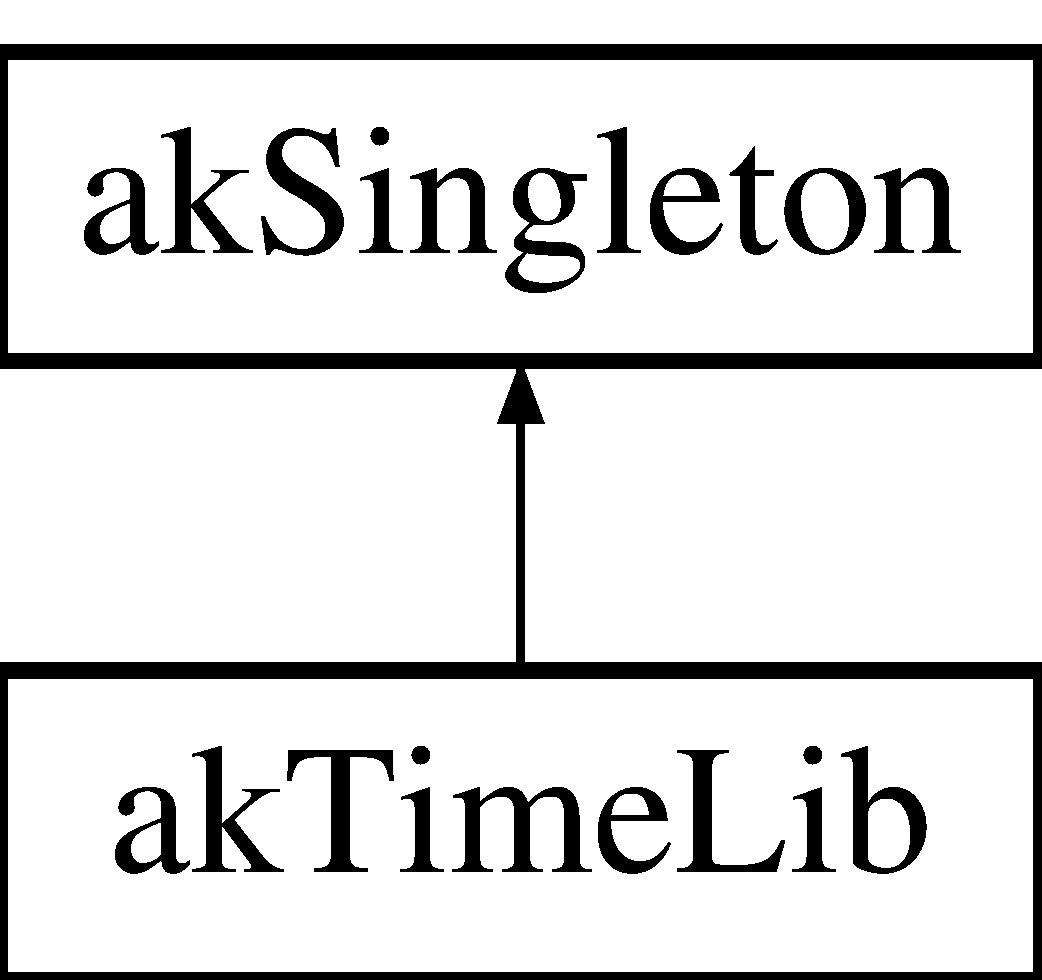
\includegraphics[height=2.000000cm]{classakTimeLib}
\end{center}
\end{figure}
\subsection*{Public Member Functions}
\begin{DoxyCompactItemize}
\item 
\hyperlink{classakTimeLib_a1ed04c2866f3216275ee5253e47e239c}{$\sim$ak\-Time\-Lib} ()
\item 
void \hyperlink{classakTimeLib_aee4282fce5f0ecdd6af03073ad158562}{init} (const char $\ast$inifile=\char`\"{}aktimelib.\-ini\char`\"{}, F\-I\-L\-E $\ast$fout=0)
\item 
void \hyperlink{classakTimeLib_a76f4e184574a8c4e4321c41e63042dd1}{dump} (F\-I\-L\-E $\ast$fout=stdout)
\item 
void \hyperlink{classakTimeLib_a3c925c111c32829c9583d5c5ae4aada2}{test} ()
\item 
time\-\_\-t \hyperlink{classakTimeLib_ae72986916166ba6ceb9dfdcb27821f3a}{convert\-G\-P\-S\-To\-U\-T\-C} (unsigned long t\-\_\-gps)
\item 
unsigned long \hyperlink{classakTimeLib_a100f532636878a9fc17f2d2ebbb56ffb}{convert\-U\-T\-C\-To\-G\-P\-S} (time\-\_\-t t\-\_\-utc)
\item 
int \hyperlink{classakTimeLib_ad96749040ca82dc93bf484bec0b840de}{is\-Leap\-Second} (unsigned long t\-\_\-gps)
\item 
int \hyperlink{classakTimeLib_a678551e52aa31b75fddfaa7716e3ad64}{n\-Leap\-Seconds} (unsigned long t\-\_\-gps)
\item 
int \hyperlink{classakTimeLib_a53076bb547d1f621530e208804eb45c6}{add\-Leap\-Second} ()
\end{DoxyCompactItemize}
\subsection*{Static Public Member Functions}
\begin{DoxyCompactItemize}
\item 
static \hyperlink{classakTimeLib}{ak\-Time\-Lib} $\ast$ \hyperlink{classakTimeLib_a60a13be5767c7e66c10e0ec9e10ad7d1}{get\-Reference} ()
\end{DoxyCompactItemize}
\subsection*{Protected Member Functions}
\begin{DoxyCompactItemize}
\item 
\hyperlink{classakTimeLib_a63e21732142b1b753a5bea511db61780}{ak\-Time\-Lib} ()
\end{DoxyCompactItemize}
\subsection*{Private Attributes}
\begin{DoxyCompactItemize}
\item 
unsigned long \hyperlink{classakTimeLib_aece53a073d766b0842004433bbb743bc}{gps\-Delay}
\item 
int \hyperlink{classakTimeLib_a1792f1ade7d43742f16880fc3747a472}{leap\-Seconds}
\item 
unsigned long \hyperlink{classakTimeLib_adc38424ed0d1365181685654c1e430dc}{next\-Leap\-Second}
\item 
unsigned long $\ast$ \hyperlink{classakTimeLib_a0e3a8f8795bb2911947530ccbfe8797f}{leap\-Sec\-Gps}
\item 
unsigned long $\ast$ \hyperlink{classakTimeLib_a9b0bc2cb3fe5d6544ef93900c00a8b96}{leap\-Sec\-Utc}
\item 
int $\ast$ \hyperlink{classakTimeLib_afb895cbc388c984925ab8ebe8361e23e}{leap\-Sec\-N}
\item 
int \hyperlink{classakTimeLib_a95186789b9668d0b3a242ac8a57bf634}{n\-Leap\-Secs}
\end{DoxyCompactItemize}
\subsection*{Static Private Attributes}
\begin{DoxyCompactItemize}
\item 
static \hyperlink{classakTimeLib}{ak\-Time\-Lib} \hyperlink{classakTimeLib_a85a5f79db7d7ddebce2174d8e7241a62}{instance}
\item 
static \hyperlink{classakSingletonCleaner}{ak\-Singleton\-Cleaner} \hyperlink{classakTimeLib_a69bc0356384bc7976926ac8c9e32847f}{cleaner}
\item 
static int \hyperlink{classakTimeLib_ad6b1a7cd89c1cccd32277b7c5442a597}{no\-Leap\-Sec\-Table} = 1
\end{DoxyCompactItemize}
\subsection*{Friends}
\begin{DoxyCompactItemize}
\item 
class \hyperlink{classakTimeLib_aa7613c42aff93f7383b7f7298e0957b9}{ak\-Singleton\-Cleaner}
\end{DoxyCompactItemize}


\subsection{Detailed Description}
Library to handle the different time formats. The class needs to reads it's basic information (about the leap seconds) from some configuration file. Before using the library the first time load these value with the function init.

The first implementation is based on a default number of leap second at the presend time and the time when the next leap second will occure. After this given occurence the ini file parameters have to be adjusted.

There are two values taken from the ini file (stanard F\-E.\-ini)\-: \begin{DoxyItemize}
\item The actual number of leap seconds (default is 13) and \item the time (in U\-T\-C format) when the next leap second is introcuded. If this value is zero no change in the leap second is considered.\end{DoxyItemize}
A sample entry is F\-E.\-ini looks like\-: 
\begin{DoxyPre}
[GPSTime]
; number of leap seconds (before nextLeapSecond - time)
leapSeconds = 13
; Time when the next leap second occures (UTC seconds)
nextLeapSecond = 1016534603
\end{DoxyPre}
 

\subsection{Constructor \& Destructor Documentation}
\hypertarget{classakTimeLib_a63e21732142b1b753a5bea511db61780}{\index{ak\-Time\-Lib@{ak\-Time\-Lib}!ak\-Time\-Lib@{ak\-Time\-Lib}}
\index{ak\-Time\-Lib@{ak\-Time\-Lib}!akTimeLib@{ak\-Time\-Lib}}
\subsubsection[{ak\-Time\-Lib}]{\setlength{\rightskip}{0pt plus 5cm}ak\-Time\-Lib\-::ak\-Time\-Lib (
\begin{DoxyParamCaption}
{}
\end{DoxyParamCaption}
)\hspace{0.3cm}{\ttfamily [protected]}}}\label{classakTimeLib_a63e21732142b1b753a5bea511db61780}
\hypertarget{classakTimeLib_a1ed04c2866f3216275ee5253e47e239c}{\index{ak\-Time\-Lib@{ak\-Time\-Lib}!$\sim$ak\-Time\-Lib@{$\sim$ak\-Time\-Lib}}
\index{$\sim$ak\-Time\-Lib@{$\sim$ak\-Time\-Lib}!akTimeLib@{ak\-Time\-Lib}}
\subsubsection[{$\sim$ak\-Time\-Lib}]{\setlength{\rightskip}{0pt plus 5cm}ak\-Time\-Lib\-::$\sim$ak\-Time\-Lib (
\begin{DoxyParamCaption}
{}
\end{DoxyParamCaption}
)\hspace{0.3cm}{\ttfamily [inline]}}}\label{classakTimeLib_a1ed04c2866f3216275ee5253e47e239c}


\subsection{Member Function Documentation}
\hypertarget{classakTimeLib_a53076bb547d1f621530e208804eb45c6}{\index{ak\-Time\-Lib@{ak\-Time\-Lib}!add\-Leap\-Second@{add\-Leap\-Second}}
\index{add\-Leap\-Second@{add\-Leap\-Second}!akTimeLib@{ak\-Time\-Lib}}
\subsubsection[{add\-Leap\-Second}]{\setlength{\rightskip}{0pt plus 5cm}int ak\-Time\-Lib\-::add\-Leap\-Second (
\begin{DoxyParamCaption}
{}
\end{DoxyParamCaption}
)}}\label{classakTimeLib_a53076bb547d1f621530e208804eb45c6}
Add new leap second \hypertarget{classakTimeLib_ae72986916166ba6ceb9dfdcb27821f3a}{\index{ak\-Time\-Lib@{ak\-Time\-Lib}!convert\-G\-P\-S\-To\-U\-T\-C@{convert\-G\-P\-S\-To\-U\-T\-C}}
\index{convert\-G\-P\-S\-To\-U\-T\-C@{convert\-G\-P\-S\-To\-U\-T\-C}!akTimeLib@{ak\-Time\-Lib}}
\subsubsection[{convert\-G\-P\-S\-To\-U\-T\-C}]{\setlength{\rightskip}{0pt plus 5cm}time\-\_\-t ak\-Time\-Lib\-::convert\-G\-P\-S\-To\-U\-T\-C (
\begin{DoxyParamCaption}
\item[{unsigned long}]{t\-\_\-gps}
\end{DoxyParamCaption}
)}}\label{classakTimeLib_ae72986916166ba6ceb9dfdcb27821f3a}
Convert the Hardware second counter the the format used by the P\-C (U\-T\-C time started at 1.\-1.\-1970)


\begin{DoxyParams}{Parameters}
{\em t\-\_\-gps} & Second counter in G\-P\-S format \\
\hline
\end{DoxyParams}
\begin{DoxyReturn}{Returns}
Time in U\-T\-C format format 
\end{DoxyReturn}
\hypertarget{classakTimeLib_a100f532636878a9fc17f2d2ebbb56ffb}{\index{ak\-Time\-Lib@{ak\-Time\-Lib}!convert\-U\-T\-C\-To\-G\-P\-S@{convert\-U\-T\-C\-To\-G\-P\-S}}
\index{convert\-U\-T\-C\-To\-G\-P\-S@{convert\-U\-T\-C\-To\-G\-P\-S}!akTimeLib@{ak\-Time\-Lib}}
\subsubsection[{convert\-U\-T\-C\-To\-G\-P\-S}]{\setlength{\rightskip}{0pt plus 5cm}unsigned long ak\-Time\-Lib\-::convert\-U\-T\-C\-To\-G\-P\-S (
\begin{DoxyParamCaption}
\item[{time\-\_\-t}]{t\-\_\-utc}
\end{DoxyParamCaption}
)}}\label{classakTimeLib_a100f532636878a9fc17f2d2ebbb56ffb}
Convert U\-T\-C to G\-P\-S time


\begin{DoxyParams}{Parameters}
{\em t\-\_\-utc} & Second counter in U\-T\-C format \\
\hline
\end{DoxyParams}
\begin{DoxyReturn}{Returns}
Time in G\-P\-S format format 
\end{DoxyReturn}
\hypertarget{classakTimeLib_a76f4e184574a8c4e4321c41e63042dd1}{\index{ak\-Time\-Lib@{ak\-Time\-Lib}!dump@{dump}}
\index{dump@{dump}!akTimeLib@{ak\-Time\-Lib}}
\subsubsection[{dump}]{\setlength{\rightskip}{0pt plus 5cm}void ak\-Time\-Lib\-::dump (
\begin{DoxyParamCaption}
\item[{F\-I\-L\-E $\ast$}]{fout = {\ttfamily stdout}}
\end{DoxyParamCaption}
)\hspace{0.3cm}{\ttfamily [inline]}}}\label{classakTimeLib_a76f4e184574a8c4e4321c41e63042dd1}
Give information about class internals \hypertarget{classakTimeLib_a60a13be5767c7e66c10e0ec9e10ad7d1}{\index{ak\-Time\-Lib@{ak\-Time\-Lib}!get\-Reference@{get\-Reference}}
\index{get\-Reference@{get\-Reference}!akTimeLib@{ak\-Time\-Lib}}
\subsubsection[{get\-Reference}]{\setlength{\rightskip}{0pt plus 5cm}{\bf ak\-Time\-Lib} $\ast$ ak\-Time\-Lib\-::get\-Reference (
\begin{DoxyParamCaption}
{}
\end{DoxyParamCaption}
)\hspace{0.3cm}{\ttfamily [static]}}}\label{classakTimeLib_a60a13be5767c7e66c10e0ec9e10ad7d1}
Get the reference to the singleton \hypertarget{classakTimeLib_aee4282fce5f0ecdd6af03073ad158562}{\index{ak\-Time\-Lib@{ak\-Time\-Lib}!init@{init}}
\index{init@{init}!akTimeLib@{ak\-Time\-Lib}}
\subsubsection[{init}]{\setlength{\rightskip}{0pt plus 5cm}void ak\-Time\-Lib\-::init (
\begin{DoxyParamCaption}
\item[{const char $\ast$}]{inifile = {\ttfamily \char`\"{}aktimelib.ini\char`\"{}}, }
\item[{F\-I\-L\-E $\ast$}]{fout = {\ttfamily 0}}
\end{DoxyParamCaption}
)}}\label{classakTimeLib_aee4282fce5f0ecdd6af03073ad158562}
Read the leap seconds table from an ini file \hypertarget{classakTimeLib_ad96749040ca82dc93bf484bec0b840de}{\index{ak\-Time\-Lib@{ak\-Time\-Lib}!is\-Leap\-Second@{is\-Leap\-Second}}
\index{is\-Leap\-Second@{is\-Leap\-Second}!akTimeLib@{ak\-Time\-Lib}}
\subsubsection[{is\-Leap\-Second}]{\setlength{\rightskip}{0pt plus 5cm}int ak\-Time\-Lib\-::is\-Leap\-Second (
\begin{DoxyParamCaption}
\item[{unsigned long}]{t\-\_\-gps}
\end{DoxyParamCaption}
)}}\label{classakTimeLib_ad96749040ca82dc93bf484bec0b840de}
Check if a gps second counter points to an leap second

\begin{DoxyReturn}{Returns}
-\/1 error, 0 no lepa second, 1 leap second 
\end{DoxyReturn}
\hypertarget{classakTimeLib_a678551e52aa31b75fddfaa7716e3ad64}{\index{ak\-Time\-Lib@{ak\-Time\-Lib}!n\-Leap\-Seconds@{n\-Leap\-Seconds}}
\index{n\-Leap\-Seconds@{n\-Leap\-Seconds}!akTimeLib@{ak\-Time\-Lib}}
\subsubsection[{n\-Leap\-Seconds}]{\setlength{\rightskip}{0pt plus 5cm}int ak\-Time\-Lib\-::n\-Leap\-Seconds (
\begin{DoxyParamCaption}
\item[{unsigned long}]{t\-\_\-gps}
\end{DoxyParamCaption}
)}}\label{classakTimeLib_a678551e52aa31b75fddfaa7716e3ad64}
Determine the number of leap seconds \hypertarget{classakTimeLib_a3c925c111c32829c9583d5c5ae4aada2}{\index{ak\-Time\-Lib@{ak\-Time\-Lib}!test@{test}}
\index{test@{test}!akTimeLib@{ak\-Time\-Lib}}
\subsubsection[{test}]{\setlength{\rightskip}{0pt plus 5cm}void ak\-Time\-Lib\-::test (
\begin{DoxyParamCaption}
{}
\end{DoxyParamCaption}
)}}\label{classakTimeLib_a3c925c111c32829c9583d5c5ae4aada2}
Test the functions of the class 

\subsection{Friends And Related Function Documentation}
\hypertarget{classakTimeLib_aa7613c42aff93f7383b7f7298e0957b9}{\index{ak\-Time\-Lib@{ak\-Time\-Lib}!ak\-Singleton\-Cleaner@{ak\-Singleton\-Cleaner}}
\index{ak\-Singleton\-Cleaner@{ak\-Singleton\-Cleaner}!akTimeLib@{ak\-Time\-Lib}}
\subsubsection[{ak\-Singleton\-Cleaner}]{\setlength{\rightskip}{0pt plus 5cm}friend class {\bf ak\-Singleton\-Cleaner}\hspace{0.3cm}{\ttfamily [friend]}}}\label{classakTimeLib_aa7613c42aff93f7383b7f7298e0957b9}


\subsection{Member Data Documentation}
\hypertarget{classakTimeLib_a69bc0356384bc7976926ac8c9e32847f}{\index{ak\-Time\-Lib@{ak\-Time\-Lib}!cleaner@{cleaner}}
\index{cleaner@{cleaner}!akTimeLib@{ak\-Time\-Lib}}
\subsubsection[{cleaner}]{\setlength{\rightskip}{0pt plus 5cm}{\bf ak\-Singleton\-Cleaner} ak\-Time\-Lib\-::cleaner\hspace{0.3cm}{\ttfamily [static]}, {\ttfamily [private]}}}\label{classakTimeLib_a69bc0356384bc7976926ac8c9e32847f}
Can the cleaner be defined in the singleton class? I fear, it will only be possible to have one singleton in a program ?! \hypertarget{classakTimeLib_aece53a073d766b0842004433bbb743bc}{\index{ak\-Time\-Lib@{ak\-Time\-Lib}!gps\-Delay@{gps\-Delay}}
\index{gps\-Delay@{gps\-Delay}!akTimeLib@{ak\-Time\-Lib}}
\subsubsection[{gps\-Delay}]{\setlength{\rightskip}{0pt plus 5cm}unsigned long ak\-Time\-Lib\-::gps\-Delay\hspace{0.3cm}{\ttfamily [private]}}}\label{classakTimeLib_aece53a073d766b0842004433bbb743bc}
Delay between G\-P\-S and U\-T\-C second count gps\-Delay = t(\-U\-T\-P) -\/ t(\-G\-P\-S) \hypertarget{classakTimeLib_a85a5f79db7d7ddebce2174d8e7241a62}{\index{ak\-Time\-Lib@{ak\-Time\-Lib}!instance@{instance}}
\index{instance@{instance}!akTimeLib@{ak\-Time\-Lib}}
\subsubsection[{instance}]{\setlength{\rightskip}{0pt plus 5cm}{\bf ak\-Time\-Lib} ak\-Time\-Lib\-::instance\hspace{0.3cm}{\ttfamily [static]}, {\ttfamily [private]}}}\label{classakTimeLib_a85a5f79db7d7ddebce2174d8e7241a62}
The only instance of this singleton class \hypertarget{classakTimeLib_a0e3a8f8795bb2911947530ccbfe8797f}{\index{ak\-Time\-Lib@{ak\-Time\-Lib}!leap\-Sec\-Gps@{leap\-Sec\-Gps}}
\index{leap\-Sec\-Gps@{leap\-Sec\-Gps}!akTimeLib@{ak\-Time\-Lib}}
\subsubsection[{leap\-Sec\-Gps}]{\setlength{\rightskip}{0pt plus 5cm}unsigned long$\ast$ ak\-Time\-Lib\-::leap\-Sec\-Gps\hspace{0.3cm}{\ttfamily [private]}}}\label{classakTimeLib_a0e3a8f8795bb2911947530ccbfe8797f}
List of gps seconds where a leap second is added \hypertarget{classakTimeLib_afb895cbc388c984925ab8ebe8361e23e}{\index{ak\-Time\-Lib@{ak\-Time\-Lib}!leap\-Sec\-N@{leap\-Sec\-N}}
\index{leap\-Sec\-N@{leap\-Sec\-N}!akTimeLib@{ak\-Time\-Lib}}
\subsubsection[{leap\-Sec\-N}]{\setlength{\rightskip}{0pt plus 5cm}int$\ast$ ak\-Time\-Lib\-::leap\-Sec\-N\hspace{0.3cm}{\ttfamily [private]}}}\label{classakTimeLib_afb895cbc388c984925ab8ebe8361e23e}
Number of leap second beginning from leap\-Sec\-Gps \hypertarget{classakTimeLib_a1792f1ade7d43742f16880fc3747a472}{\index{ak\-Time\-Lib@{ak\-Time\-Lib}!leap\-Seconds@{leap\-Seconds}}
\index{leap\-Seconds@{leap\-Seconds}!akTimeLib@{ak\-Time\-Lib}}
\subsubsection[{leap\-Seconds}]{\setlength{\rightskip}{0pt plus 5cm}int ak\-Time\-Lib\-::leap\-Seconds\hspace{0.3cm}{\ttfamily [private]}}}\label{classakTimeLib_a1792f1ade7d43742f16880fc3747a472}
Number of actual leap seconds \hypertarget{classakTimeLib_a9b0bc2cb3fe5d6544ef93900c00a8b96}{\index{ak\-Time\-Lib@{ak\-Time\-Lib}!leap\-Sec\-Utc@{leap\-Sec\-Utc}}
\index{leap\-Sec\-Utc@{leap\-Sec\-Utc}!akTimeLib@{ak\-Time\-Lib}}
\subsubsection[{leap\-Sec\-Utc}]{\setlength{\rightskip}{0pt plus 5cm}unsigned long$\ast$ ak\-Time\-Lib\-::leap\-Sec\-Utc\hspace{0.3cm}{\ttfamily [private]}}}\label{classakTimeLib_a9b0bc2cb3fe5d6544ef93900c00a8b96}
List of utc/ntp second where a leap second is added \hypertarget{classakTimeLib_adc38424ed0d1365181685654c1e430dc}{\index{ak\-Time\-Lib@{ak\-Time\-Lib}!next\-Leap\-Second@{next\-Leap\-Second}}
\index{next\-Leap\-Second@{next\-Leap\-Second}!akTimeLib@{ak\-Time\-Lib}}
\subsubsection[{next\-Leap\-Second}]{\setlength{\rightskip}{0pt plus 5cm}unsigned long ak\-Time\-Lib\-::next\-Leap\-Second\hspace{0.3cm}{\ttfamily [private]}}}\label{classakTimeLib_adc38424ed0d1365181685654c1e430dc}
Time when the next leap second occures. This time has to be given in U\-T\-C seconds. \hypertarget{classakTimeLib_a95186789b9668d0b3a242ac8a57bf634}{\index{ak\-Time\-Lib@{ak\-Time\-Lib}!n\-Leap\-Secs@{n\-Leap\-Secs}}
\index{n\-Leap\-Secs@{n\-Leap\-Secs}!akTimeLib@{ak\-Time\-Lib}}
\subsubsection[{n\-Leap\-Secs}]{\setlength{\rightskip}{0pt plus 5cm}int ak\-Time\-Lib\-::n\-Leap\-Secs\hspace{0.3cm}{\ttfamily [private]}}}\label{classakTimeLib_a95186789b9668d0b3a242ac8a57bf634}
Number of entries in the leap list \hypertarget{classakTimeLib_ad6b1a7cd89c1cccd32277b7c5442a597}{\index{ak\-Time\-Lib@{ak\-Time\-Lib}!no\-Leap\-Sec\-Table@{no\-Leap\-Sec\-Table}}
\index{no\-Leap\-Sec\-Table@{no\-Leap\-Sec\-Table}!akTimeLib@{ak\-Time\-Lib}}
\subsubsection[{no\-Leap\-Sec\-Table}]{\setlength{\rightskip}{0pt plus 5cm}int ak\-Time\-Lib\-::no\-Leap\-Sec\-Table = 1\hspace{0.3cm}{\ttfamily [static]}, {\ttfamily [private]}}}\label{classakTimeLib_ad6b1a7cd89c1cccd32277b7c5442a597}
Flag to show if leap second table is missing 

The documentation for this class was generated from the following files\-:\begin{DoxyCompactItemize}
\item 
/home/ntj/\-Development/phd/kitcube-\/tools/src/akutil/\hyperlink{aktimelib_8h}{aktimelib.\-h}\item 
/home/ntj/\-Development/phd/kitcube-\/tools/src/akutil/\hyperlink{aktimelib_8cpp}{aktimelib.\-cpp}\end{DoxyCompactItemize}

\hypertarget{classanalyseMatrix}{\section{analyse\-Matrix Class Reference}
\label{classanalyseMatrix}\index{analyse\-Matrix@{analyse\-Matrix}}
}


{\ttfamily \#include $<$analysematrix.\-h$>$}

\subsection*{Public Member Functions}
\begin{DoxyCompactItemize}
\item 
\hyperlink{classanalyseMatrix_ae056d1b34e217c935a4353255ebdd9bb}{analyse\-Matrix} ()
\item 
\hyperlink{classanalyseMatrix_ab0bad30e89e799510fbb95a5b9d37ab8}{$\sim$analyse\-Matrix} ()
\item 
void \hyperlink{classanalyseMatrix_a39fd86f43c32f0803d8e05859e96afaa}{filter\-By2x2} (int filter\mbox{[}2\mbox{]}\mbox{[}2\mbox{]}, int col, int row, double matrix\mbox{[}20\mbox{]}\mbox{[}22\mbox{]}, double res\mbox{[}20\mbox{]}\mbox{[}22\mbox{]}, int mask\mbox{[}20\mbox{]}\mbox{[}22\mbox{]})
\item 
void \hyperlink{classanalyseMatrix_af376bbf6f497ebe891aa1670072008a9}{display\-Matrix} (F\-I\-L\-E $\ast$fout, double matrix\mbox{[}20\mbox{]}\mbox{[}22\mbox{]}, const char $\ast$title)
\item 
void \hyperlink{classanalyseMatrix_a455fced75f8847d2749111da7e7fd44a}{display\-Matrix} (F\-I\-L\-E $\ast$fout, int matrix\mbox{[}20\mbox{]}\mbox{[}22\mbox{]}, const char $\ast$title, int norm=0, int value=0, const char $\ast$tag=0)
\item 
int \hyperlink{classanalyseMatrix_a7f26b3aefa10cb9457c3dd3d2334420d}{display\-Pixel\-List} (F\-I\-L\-E $\ast$fout, int matrix\mbox{[}20\mbox{]}\mbox{[}22\mbox{]})
\item 
void \hyperlink{classanalyseMatrix_a6ff734ef0f617117e1dd9235646edc1a}{classify\-By\-Threshold} (double thresh, double matrix\mbox{[}20\mbox{]}\mbox{[}22\mbox{]}, int res\mbox{[}20\mbox{]}\mbox{[}22\mbox{]}, int up=1)
\item 
void \hyperlink{classanalyseMatrix_a16bc8177a6cfbf2bc8877c4bfa890ef3}{set\-Matrix} (double value, double matrix\mbox{[}20\mbox{]}\mbox{[}22\mbox{]})
\item 
void \hyperlink{classanalyseMatrix_acbcd251fd377f28de7ca6a1381b519cf}{set\-Matrix} (int value, int matrix\mbox{[}20\mbox{]}\mbox{[}22\mbox{]})
\item 
void \hyperlink{classanalyseMatrix_ab6daa3c332d14b9d71b1208edfdf33cf}{mult\-Matrix} (double value, double matrix\mbox{[}20\mbox{]}\mbox{[}22\mbox{]})
\item 
void \hyperlink{classanalyseMatrix_a756d6af7a102bf5624589b118307b935}{mult\-Mask} (int value, int mask\mbox{[}20\mbox{]}\mbox{[}22\mbox{]})
\item 
void \hyperlink{classanalyseMatrix_ac1fa43f05dbc70125df4c63dcb65df29}{div\-Matrix} (double res\mbox{[}20\mbox{]}\mbox{[}22\mbox{]}, double matrix\mbox{[}20\mbox{]}\mbox{[}22\mbox{]})
\item 
void \hyperlink{classanalyseMatrix_a1f0cbad7de61b574221f1fddac3252e7}{div\-Matrix} (double res\mbox{[}20\mbox{]}\mbox{[}22\mbox{]}, int matrix\mbox{[}20\mbox{]}\mbox{[}22\mbox{]})
\item 
void \hyperlink{classanalyseMatrix_acb6421a2e698a280e19d751feca9faff}{mean\-Matrix} (double matrix\mbox{[}20\mbox{]}\mbox{[}22\mbox{]}, double $\ast$mean, double $\ast$var, int $\ast$n, int mask\mbox{[}20\mbox{]}\mbox{[}22\mbox{]})
\item 
void \hyperlink{classanalyseMatrix_a4ca419c0a8d92accfcd2ef1660497378}{mean\-Matrix} (double matrix\mbox{[}20\mbox{]}\mbox{[}22\mbox{]}, double $\ast$mean, double $\ast$var, int $\ast$n, int mask\mbox{[}20\mbox{]}\mbox{[}22\mbox{]}, int err\mbox{[}20\mbox{]}\mbox{[}22\mbox{]})
\item 
void \hyperlink{classanalyseMatrix_a25918ce9812bc346425cdcdb3d1f72bd}{add\-Mask} (int res\mbox{[}20\mbox{]}\mbox{[}22\mbox{]}, int mask\mbox{[}20\mbox{]}\mbox{[}22\mbox{]})
\item 
void \hyperlink{classanalyseMatrix_a821b829a991ad53d8b068d00ec411405}{add\-Matrix} (double res\mbox{[}20\mbox{]}\mbox{[}22\mbox{]}, double matrix\mbox{[}20\mbox{]}\mbox{[}22\mbox{]})
\item 
void \hyperlink{classanalyseMatrix_ae561bd929c3d2a0ceb1f3f1139bc533f}{copy\-Matrix} (double res\mbox{[}20\mbox{]}\mbox{[}22\mbox{]}, double matrix\mbox{[}20\mbox{]}\mbox{[}22\mbox{]})
\item 
void \hyperlink{classanalyseMatrix_a779d81ad2a1991688dfddde7011d6d06}{or\-Mask} (int res\mbox{[}20\mbox{]}\mbox{[}22\mbox{]}, int mask\mbox{[}20\mbox{]}\mbox{[}22\mbox{]})
\item 
void \hyperlink{classanalyseMatrix_aa454eb316f95fca25b72073020e04e36}{invert\-Mask} (int mask\mbox{[}20\mbox{]}\mbox{[}22\mbox{]})
\item 
int \hyperlink{classanalyseMatrix_a8c70c1c16f2482328b5bdc3e7b792034}{n\-Mask} (int mask\mbox{[}20\mbox{]}\mbox{[}22\mbox{]})
\item 
void \hyperlink{classanalyseMatrix_ae42ccc44ff5a297121c7e73a6b4eadbf}{copy\-Mask} (int res\mbox{[}20\mbox{]}\mbox{[}22\mbox{]}, int mask\mbox{[}20\mbox{]}\mbox{[}22\mbox{]})
\item 
void \hyperlink{classanalyseMatrix_a4820924cab97d5a6bce8a66766b8a4f5}{max\-Mask} (int max, int mask\mbox{[}20\mbox{]}\mbox{[}22\mbox{]})
\item 
void \hyperlink{classanalyseMatrix_abfe8bf706868c42cfb8cf2dac9c2d0d4}{min\-Mask} (int min, int mask\mbox{[}20\mbox{]}\mbox{[}22\mbox{]})
\item 
void \hyperlink{classanalyseMatrix_a8f3afe9804ef7e5a15b805a7742faecc}{find\-High\-Noise1} (F\-I\-L\-E $\ast$fout, double matrix\mbox{[}20\mbox{]}\mbox{[}22\mbox{]}, int res\mbox{[}20\mbox{]}\mbox{[}22\mbox{]}, int err\mbox{[}20\mbox{]}\mbox{[}22\mbox{]})
\item 
void \hyperlink{classanalyseMatrix_a81f17c9773ff663a24095af3a8a8700b}{find\-High\-Noise2} (F\-I\-L\-E $\ast$fout, double matrix\mbox{[}20\mbox{]}\mbox{[}22\mbox{]}, int res\mbox{[}20\mbox{]}\mbox{[}22\mbox{]}, int err\mbox{[}20\mbox{]}\mbox{[}22\mbox{]})
\item 
void \hyperlink{classanalyseMatrix_a53f84ec658a8a2826ef26876091706a0}{clear\-Noisy\-Pixel} ()
\item 
void \hyperlink{classanalyseMatrix_a74d13c1dffb2d2795b583db6b88026e9}{clear\-Faulty\-Pixel} ()
\item 
void \hyperlink{classanalyseMatrix_a0f00e198a9f2005d6a6ca5f4fe70fda2}{add\-Noisy\-Pixel} (int mask\mbox{[}20\mbox{]}\mbox{[}22\mbox{]})
\item 
void \hyperlink{classanalyseMatrix_abc6c434b1e9c2dccebf7380b2237cd14}{find\-High\-Noise} (F\-I\-L\-E $\ast$fout, double matrix\mbox{[}20\mbox{]}\mbox{[}22\mbox{]})
\item 
void \hyperlink{classanalyseMatrix_a4b69db0536063f67fd7ed635953d08b4}{mean\-Of\-Normal\-Pixel} (double matrix\mbox{[}20\mbox{]}\mbox{[}22\mbox{]}, double $\ast$mean, double $\ast$var, int $\ast$n)
\item 
void \hyperlink{classanalyseMatrix_af32477590ff3d201d3d9ab3faed270a2}{mean\-Of\-Noisy\-Pixel} (double matrix\mbox{[}20\mbox{]}\mbox{[}22\mbox{]}, double $\ast$mean, double $\ast$var, int $\ast$n)
\item 
int \hyperlink{classanalyseMatrix_a9db1346d6a0601e0863961dddd310508}{n\-Noisy\-Pixel} ()
\item 
void \hyperlink{classanalyseMatrix_a953d8a856b95876b5f7e90e25063310b}{display\-Noisy\-Pixel\-List} (F\-I\-L\-E $\ast$fout)
\end{DoxyCompactItemize}
\subsection*{Public Attributes}
\begin{DoxyCompactItemize}
\item 
int \hyperlink{classanalyseMatrix_a7309694bc069cc545ddb80de2cf96cb8}{noisy\-Pixel} \mbox{[}20\mbox{]}\mbox{[}22\mbox{]}
\item 
int \hyperlink{classanalyseMatrix_ae1a917330c3aa0e9ee6446d14f31eed3}{noisy\-Pixel\-Last} \mbox{[}20\mbox{]}\mbox{[}22\mbox{]}
\item 
int \hyperlink{classanalyseMatrix_a8cddd52641a8d1dc2a6cf669584ac440}{faulty\-Pixel} \mbox{[}20\mbox{]}\mbox{[}22\mbox{]}
\item 
int \hyperlink{classanalyseMatrix_af4911f335c7415683cac99607ee3972d}{noisy\-Runs}
\item 
double \hyperlink{classanalyseMatrix_a1e35cc039abe9757861c13ad48b73134}{noisy\-N\-Variances}
\item 
int \hyperlink{classanalyseMatrix_adb3542dfa480b47bdc51442a1980821a}{noisy\-Min\-Variance}
\item 
double \hyperlink{classanalyseMatrix_a8a8c6af9d824a68930c5307517e050f5}{noisy\-Neighbor\-Diff}
\item 
double \hyperlink{classanalyseMatrix_ab2c3e6805f8c69bb1c2317df1130cffd}{noisy\-Abs\-Thresh}
\item 
double \hyperlink{classanalyseMatrix_a66744956a995f194e5a018da3aaedc12}{noisy\-Low\-Thresh}
\item 
int \hyperlink{classanalyseMatrix_a5c3dd03672f12a8a3ad1adbbe15d3a3e}{debug}
\end{DoxyCompactItemize}


\subsection{Detailed Description}
Analyse the variance matrix of a telescope All functions are on matrices of 20x22 elements. 

\subsection{Constructor \& Destructor Documentation}
\hypertarget{classanalyseMatrix_ae056d1b34e217c935a4353255ebdd9bb}{\index{analyse\-Matrix@{analyse\-Matrix}!analyse\-Matrix@{analyse\-Matrix}}
\index{analyse\-Matrix@{analyse\-Matrix}!analyseMatrix@{analyse\-Matrix}}
\subsubsection[{analyse\-Matrix}]{\setlength{\rightskip}{0pt plus 5cm}analyse\-Matrix\-::analyse\-Matrix (
\begin{DoxyParamCaption}
{}
\end{DoxyParamCaption}
)}}\label{classanalyseMatrix_ae056d1b34e217c935a4353255ebdd9bb}
\hypertarget{classanalyseMatrix_ab0bad30e89e799510fbb95a5b9d37ab8}{\index{analyse\-Matrix@{analyse\-Matrix}!$\sim$analyse\-Matrix@{$\sim$analyse\-Matrix}}
\index{$\sim$analyse\-Matrix@{$\sim$analyse\-Matrix}!analyseMatrix@{analyse\-Matrix}}
\subsubsection[{$\sim$analyse\-Matrix}]{\setlength{\rightskip}{0pt plus 5cm}analyse\-Matrix\-::$\sim$analyse\-Matrix (
\begin{DoxyParamCaption}
{}
\end{DoxyParamCaption}
)}}\label{classanalyseMatrix_ab0bad30e89e799510fbb95a5b9d37ab8}


\subsection{Member Function Documentation}
\hypertarget{classanalyseMatrix_a25918ce9812bc346425cdcdb3d1f72bd}{\index{analyse\-Matrix@{analyse\-Matrix}!add\-Mask@{add\-Mask}}
\index{add\-Mask@{add\-Mask}!analyseMatrix@{analyse\-Matrix}}
\subsubsection[{add\-Mask}]{\setlength{\rightskip}{0pt plus 5cm}void analyse\-Matrix\-::add\-Mask (
\begin{DoxyParamCaption}
\item[{int}]{res\mbox{[}20\mbox{]}\mbox{[}22\mbox{]}, }
\item[{int}]{mask\mbox{[}20\mbox{]}\mbox{[}22\mbox{]}}
\end{DoxyParamCaption}
)}}\label{classanalyseMatrix_a25918ce9812bc346425cdcdb3d1f72bd}
Add two masks \hypertarget{classanalyseMatrix_a821b829a991ad53d8b068d00ec411405}{\index{analyse\-Matrix@{analyse\-Matrix}!add\-Matrix@{add\-Matrix}}
\index{add\-Matrix@{add\-Matrix}!analyseMatrix@{analyse\-Matrix}}
\subsubsection[{add\-Matrix}]{\setlength{\rightskip}{0pt plus 5cm}void analyse\-Matrix\-::add\-Matrix (
\begin{DoxyParamCaption}
\item[{double}]{res\mbox{[}20\mbox{]}\mbox{[}22\mbox{]}, }
\item[{double}]{matrix\mbox{[}20\mbox{]}\mbox{[}22\mbox{]}}
\end{DoxyParamCaption}
)}}\label{classanalyseMatrix_a821b829a991ad53d8b068d00ec411405}
Add two matrixes \hypertarget{classanalyseMatrix_a0f00e198a9f2005d6a6ca5f4fe70fda2}{\index{analyse\-Matrix@{analyse\-Matrix}!add\-Noisy\-Pixel@{add\-Noisy\-Pixel}}
\index{add\-Noisy\-Pixel@{add\-Noisy\-Pixel}!analyseMatrix@{analyse\-Matrix}}
\subsubsection[{add\-Noisy\-Pixel}]{\setlength{\rightskip}{0pt plus 5cm}void analyse\-Matrix\-::add\-Noisy\-Pixel (
\begin{DoxyParamCaption}
\item[{int}]{mask\mbox{[}20\mbox{]}\mbox{[}22\mbox{]}}
\end{DoxyParamCaption}
)}}\label{classanalyseMatrix_a0f00e198a9f2005d6a6ca5f4fe70fda2}
Add a new noisy pixel mask \hypertarget{classanalyseMatrix_a6ff734ef0f617117e1dd9235646edc1a}{\index{analyse\-Matrix@{analyse\-Matrix}!classify\-By\-Threshold@{classify\-By\-Threshold}}
\index{classify\-By\-Threshold@{classify\-By\-Threshold}!analyseMatrix@{analyse\-Matrix}}
\subsubsection[{classify\-By\-Threshold}]{\setlength{\rightskip}{0pt plus 5cm}void analyse\-Matrix\-::classify\-By\-Threshold (
\begin{DoxyParamCaption}
\item[{double}]{thresh, }
\item[{double}]{matrix\mbox{[}20\mbox{]}\mbox{[}22\mbox{]}, }
\item[{int}]{res\mbox{[}20\mbox{]}\mbox{[}22\mbox{]}, }
\item[{int}]{up = {\ttfamily 1}}
\end{DoxyParamCaption}
)}}\label{classanalyseMatrix_a6ff734ef0f617117e1dd9235646edc1a}
Classify by using a constant threshold matrix, res and mask are 20x22 pixel. The up parameter controls whether the values higher or lower of the threshold should be taken. \hypertarget{classanalyseMatrix_a74d13c1dffb2d2795b583db6b88026e9}{\index{analyse\-Matrix@{analyse\-Matrix}!clear\-Faulty\-Pixel@{clear\-Faulty\-Pixel}}
\index{clear\-Faulty\-Pixel@{clear\-Faulty\-Pixel}!analyseMatrix@{analyse\-Matrix}}
\subsubsection[{clear\-Faulty\-Pixel}]{\setlength{\rightskip}{0pt plus 5cm}void analyse\-Matrix\-::clear\-Faulty\-Pixel (
\begin{DoxyParamCaption}
{}
\end{DoxyParamCaption}
)}}\label{classanalyseMatrix_a74d13c1dffb2d2795b583db6b88026e9}
Clear faulty pixel matrix \hypertarget{classanalyseMatrix_a53f84ec658a8a2826ef26876091706a0}{\index{analyse\-Matrix@{analyse\-Matrix}!clear\-Noisy\-Pixel@{clear\-Noisy\-Pixel}}
\index{clear\-Noisy\-Pixel@{clear\-Noisy\-Pixel}!analyseMatrix@{analyse\-Matrix}}
\subsubsection[{clear\-Noisy\-Pixel}]{\setlength{\rightskip}{0pt plus 5cm}void analyse\-Matrix\-::clear\-Noisy\-Pixel (
\begin{DoxyParamCaption}
{}
\end{DoxyParamCaption}
)}}\label{classanalyseMatrix_a53f84ec658a8a2826ef26876091706a0}
Clear noisy pixel matrix \hypertarget{classanalyseMatrix_ae42ccc44ff5a297121c7e73a6b4eadbf}{\index{analyse\-Matrix@{analyse\-Matrix}!copy\-Mask@{copy\-Mask}}
\index{copy\-Mask@{copy\-Mask}!analyseMatrix@{analyse\-Matrix}}
\subsubsection[{copy\-Mask}]{\setlength{\rightskip}{0pt plus 5cm}void analyse\-Matrix\-::copy\-Mask (
\begin{DoxyParamCaption}
\item[{int}]{res\mbox{[}20\mbox{]}\mbox{[}22\mbox{]}, }
\item[{int}]{mask\mbox{[}20\mbox{]}\mbox{[}22\mbox{]}}
\end{DoxyParamCaption}
)}}\label{classanalyseMatrix_ae42ccc44ff5a297121c7e73a6b4eadbf}
Copy the mask to res \hypertarget{classanalyseMatrix_ae561bd929c3d2a0ceb1f3f1139bc533f}{\index{analyse\-Matrix@{analyse\-Matrix}!copy\-Matrix@{copy\-Matrix}}
\index{copy\-Matrix@{copy\-Matrix}!analyseMatrix@{analyse\-Matrix}}
\subsubsection[{copy\-Matrix}]{\setlength{\rightskip}{0pt plus 5cm}void analyse\-Matrix\-::copy\-Matrix (
\begin{DoxyParamCaption}
\item[{double}]{res\mbox{[}20\mbox{]}\mbox{[}22\mbox{]}, }
\item[{double}]{matrix\mbox{[}20\mbox{]}\mbox{[}22\mbox{]}}
\end{DoxyParamCaption}
)}}\label{classanalyseMatrix_ae561bd929c3d2a0ceb1f3f1139bc533f}
Copy matrix to res \hypertarget{classanalyseMatrix_af376bbf6f497ebe891aa1670072008a9}{\index{analyse\-Matrix@{analyse\-Matrix}!display\-Matrix@{display\-Matrix}}
\index{display\-Matrix@{display\-Matrix}!analyseMatrix@{analyse\-Matrix}}
\subsubsection[{display\-Matrix}]{\setlength{\rightskip}{0pt plus 5cm}void analyse\-Matrix\-::display\-Matrix (
\begin{DoxyParamCaption}
\item[{F\-I\-L\-E $\ast$}]{fout, }
\item[{double}]{matrix\mbox{[}20\mbox{]}\mbox{[}22\mbox{]}, }
\item[{const char $\ast$}]{title}
\end{DoxyParamCaption}
)}}\label{classanalyseMatrix_af376bbf6f497ebe891aa1670072008a9}
Display a matrix of 20x22 elements \hypertarget{classanalyseMatrix_a455fced75f8847d2749111da7e7fd44a}{\index{analyse\-Matrix@{analyse\-Matrix}!display\-Matrix@{display\-Matrix}}
\index{display\-Matrix@{display\-Matrix}!analyseMatrix@{analyse\-Matrix}}
\subsubsection[{display\-Matrix}]{\setlength{\rightskip}{0pt plus 5cm}void analyse\-Matrix\-::display\-Matrix (
\begin{DoxyParamCaption}
\item[{F\-I\-L\-E $\ast$}]{fout, }
\item[{int}]{matrix\mbox{[}20\mbox{]}\mbox{[}22\mbox{]}, }
\item[{const char $\ast$}]{title, }
\item[{int}]{norm = {\ttfamily 0}, }
\item[{int}]{value = {\ttfamily 0}, }
\item[{const char $\ast$}]{tag = {\ttfamily 0}}
\end{DoxyParamCaption}
)}}\label{classanalyseMatrix_a455fced75f8847d2749111da7e7fd44a}
Display a matrix of 20x22 integer elements. With the argument norm $>$ 0, relative values in percent a the normation given will be displayed. A special value can be replaced by a tag. \hypertarget{classanalyseMatrix_a953d8a856b95876b5f7e90e25063310b}{\index{analyse\-Matrix@{analyse\-Matrix}!display\-Noisy\-Pixel\-List@{display\-Noisy\-Pixel\-List}}
\index{display\-Noisy\-Pixel\-List@{display\-Noisy\-Pixel\-List}!analyseMatrix@{analyse\-Matrix}}
\subsubsection[{display\-Noisy\-Pixel\-List}]{\setlength{\rightskip}{0pt plus 5cm}void analyse\-Matrix\-::display\-Noisy\-Pixel\-List (
\begin{DoxyParamCaption}
\item[{F\-I\-L\-E $\ast$}]{fout}
\end{DoxyParamCaption}
)}}\label{classanalyseMatrix_a953d8a856b95876b5f7e90e25063310b}
Display the list of noisy pixel in the last analysis \hypertarget{classanalyseMatrix_a7f26b3aefa10cb9457c3dd3d2334420d}{\index{analyse\-Matrix@{analyse\-Matrix}!display\-Pixel\-List@{display\-Pixel\-List}}
\index{display\-Pixel\-List@{display\-Pixel\-List}!analyseMatrix@{analyse\-Matrix}}
\subsubsection[{display\-Pixel\-List}]{\setlength{\rightskip}{0pt plus 5cm}int analyse\-Matrix\-::display\-Pixel\-List (
\begin{DoxyParamCaption}
\item[{F\-I\-L\-E $\ast$}]{fout, }
\item[{int}]{matrix\mbox{[}20\mbox{]}\mbox{[}22\mbox{]}}
\end{DoxyParamCaption}
)}}\label{classanalyseMatrix_a7f26b3aefa10cb9457c3dd3d2334420d}
Display list of coordinates of all pixel in the mask Returns the number of pixel in the mask \hypertarget{classanalyseMatrix_ac1fa43f05dbc70125df4c63dcb65df29}{\index{analyse\-Matrix@{analyse\-Matrix}!div\-Matrix@{div\-Matrix}}
\index{div\-Matrix@{div\-Matrix}!analyseMatrix@{analyse\-Matrix}}
\subsubsection[{div\-Matrix}]{\setlength{\rightskip}{0pt plus 5cm}void analyse\-Matrix\-::div\-Matrix (
\begin{DoxyParamCaption}
\item[{double}]{res\mbox{[}20\mbox{]}\mbox{[}22\mbox{]}, }
\item[{double}]{matrix\mbox{[}20\mbox{]}\mbox{[}22\mbox{]}}
\end{DoxyParamCaption}
)}}\label{classanalyseMatrix_ac1fa43f05dbc70125df4c63dcb65df29}
Devide by matrix \hypertarget{classanalyseMatrix_a1f0cbad7de61b574221f1fddac3252e7}{\index{analyse\-Matrix@{analyse\-Matrix}!div\-Matrix@{div\-Matrix}}
\index{div\-Matrix@{div\-Matrix}!analyseMatrix@{analyse\-Matrix}}
\subsubsection[{div\-Matrix}]{\setlength{\rightskip}{0pt plus 5cm}void analyse\-Matrix\-::div\-Matrix (
\begin{DoxyParamCaption}
\item[{double}]{res\mbox{[}20\mbox{]}\mbox{[}22\mbox{]}, }
\item[{int}]{matrix\mbox{[}20\mbox{]}\mbox{[}22\mbox{]}}
\end{DoxyParamCaption}
)}}\label{classanalyseMatrix_a1f0cbad7de61b574221f1fddac3252e7}
Devide by matrix \hypertarget{classanalyseMatrix_a39fd86f43c32f0803d8e05859e96afaa}{\index{analyse\-Matrix@{analyse\-Matrix}!filter\-By2x2@{filter\-By2x2}}
\index{filter\-By2x2@{filter\-By2x2}!analyseMatrix@{analyse\-Matrix}}
\subsubsection[{filter\-By2x2}]{\setlength{\rightskip}{0pt plus 5cm}void analyse\-Matrix\-::filter\-By2x2 (
\begin{DoxyParamCaption}
\item[{int}]{filter\mbox{[}2\mbox{]}\mbox{[}2\mbox{]}, }
\item[{int}]{col, }
\item[{int}]{row, }
\item[{double}]{matrix\mbox{[}20\mbox{]}\mbox{[}22\mbox{]}, }
\item[{double}]{res\mbox{[}20\mbox{]}\mbox{[}22\mbox{]}, }
\item[{int}]{mask\mbox{[}20\mbox{]}\mbox{[}22\mbox{]}}
\end{DoxyParamCaption}
)}}\label{classanalyseMatrix_a39fd86f43c32f0803d8e05859e96afaa}
Filter a matrix using a free 2x2 matrix. With mask pixel can be excluded from the calculation matrix, res and mask are 20x22 pixel Parameters (col/row) determine the center pixel of the filter. Possible values are col, row = \{0$|$1\}. \hypertarget{classanalyseMatrix_abc6c434b1e9c2dccebf7380b2237cd14}{\index{analyse\-Matrix@{analyse\-Matrix}!find\-High\-Noise@{find\-High\-Noise}}
\index{find\-High\-Noise@{find\-High\-Noise}!analyseMatrix@{analyse\-Matrix}}
\subsubsection[{find\-High\-Noise}]{\setlength{\rightskip}{0pt plus 5cm}void analyse\-Matrix\-::find\-High\-Noise (
\begin{DoxyParamCaption}
\item[{F\-I\-L\-E $\ast$}]{fout, }
\item[{double}]{matrix\mbox{[}20\mbox{]}\mbox{[}22\mbox{]}}
\end{DoxyParamCaption}
)}}\label{classanalyseMatrix_abc6c434b1e9c2dccebf7380b2237cd14}
Analyse matrix and store result in the local arrays \hypertarget{classanalyseMatrix_a8f3afe9804ef7e5a15b805a7742faecc}{\index{analyse\-Matrix@{analyse\-Matrix}!find\-High\-Noise1@{find\-High\-Noise1}}
\index{find\-High\-Noise1@{find\-High\-Noise1}!analyseMatrix@{analyse\-Matrix}}
\subsubsection[{find\-High\-Noise1}]{\setlength{\rightskip}{0pt plus 5cm}void analyse\-Matrix\-::find\-High\-Noise1 (
\begin{DoxyParamCaption}
\item[{F\-I\-L\-E $\ast$}]{fout, }
\item[{double}]{matrix\mbox{[}20\mbox{]}\mbox{[}22\mbox{]}, }
\item[{int}]{res\mbox{[}20\mbox{]}\mbox{[}22\mbox{]}, }
\item[{int}]{err\mbox{[}20\mbox{]}\mbox{[}22\mbox{]}}
\end{DoxyParamCaption}
)}}\label{classanalyseMatrix_a8f3afe9804ef7e5a15b805a7742faecc}
Automatically find pixel with high noise in the variance matrix

Algorithm\-:
\begin{DoxyItemize}
\item Calculate statistics of pixel distribution
\item Take threshold proportional to N times the distribution variance. Consider a minumum threshold.
\item Repeat the algorithm taking only non noisy pixel into account.
\end{DoxyItemize}

Parameter of the alorithm\-:
\begin{DoxyItemize}
\item Factor N of the variances \mbox{[}-\/\mbox{]}
\item Minimum threshold \mbox{[}A\-D\-C Counts\mbox{]} 
\end{DoxyItemize}\hypertarget{classanalyseMatrix_a81f17c9773ff663a24095af3a8a8700b}{\index{analyse\-Matrix@{analyse\-Matrix}!find\-High\-Noise2@{find\-High\-Noise2}}
\index{find\-High\-Noise2@{find\-High\-Noise2}!analyseMatrix@{analyse\-Matrix}}
\subsubsection[{find\-High\-Noise2}]{\setlength{\rightskip}{0pt plus 5cm}void analyse\-Matrix\-::find\-High\-Noise2 (
\begin{DoxyParamCaption}
\item[{F\-I\-L\-E $\ast$}]{fout, }
\item[{double}]{matrix\mbox{[}20\mbox{]}\mbox{[}22\mbox{]}, }
\item[{int}]{res\mbox{[}20\mbox{]}\mbox{[}22\mbox{]}, }
\item[{int}]{err\mbox{[}20\mbox{]}\mbox{[}22\mbox{]}}
\end{DoxyParamCaption}
)}}\label{classanalyseMatrix_a81f17c9773ff663a24095af3a8a8700b}
Automatically find pixel with high noise in the variance matrix

Algorithm\-:
\begin{DoxyItemize}
\item Find all negative values and exclude from further analsysis
\item Run a 2x2 edge filters over the pixel matrix.
\item Use a threshold on the difference matrix.
\item Repeat this rotating the 2x2 filter to consider all orientations. and overlap the resulting pixel mask.
\item Calculate the distribution mean for low and high noise pixel
\item Use a threshold on the orignal distribution. The thresold is choosen to mean high noise value minus half of the difference image threshold. Add the results.
\end{DoxyItemize}

Parameter of the algorithm\-:
\begin{DoxyItemize}
\item Threshold in the difference matrixes 
\end{DoxyItemize}\hypertarget{classanalyseMatrix_aa454eb316f95fca25b72073020e04e36}{\index{analyse\-Matrix@{analyse\-Matrix}!invert\-Mask@{invert\-Mask}}
\index{invert\-Mask@{invert\-Mask}!analyseMatrix@{analyse\-Matrix}}
\subsubsection[{invert\-Mask}]{\setlength{\rightskip}{0pt plus 5cm}void analyse\-Matrix\-::invert\-Mask (
\begin{DoxyParamCaption}
\item[{int}]{mask\mbox{[}20\mbox{]}\mbox{[}22\mbox{]}}
\end{DoxyParamCaption}
)}}\label{classanalyseMatrix_aa454eb316f95fca25b72073020e04e36}
Invert the values of the mask \hypertarget{classanalyseMatrix_a4820924cab97d5a6bce8a66766b8a4f5}{\index{analyse\-Matrix@{analyse\-Matrix}!max\-Mask@{max\-Mask}}
\index{max\-Mask@{max\-Mask}!analyseMatrix@{analyse\-Matrix}}
\subsubsection[{max\-Mask}]{\setlength{\rightskip}{0pt plus 5cm}void analyse\-Matrix\-::max\-Mask (
\begin{DoxyParamCaption}
\item[{int}]{max, }
\item[{int}]{mask\mbox{[}20\mbox{]}\mbox{[}22\mbox{]}}
\end{DoxyParamCaption}
)}}\label{classanalyseMatrix_a4820924cab97d5a6bce8a66766b8a4f5}
Maximum of constant and mask values \hypertarget{classanalyseMatrix_acb6421a2e698a280e19d751feca9faff}{\index{analyse\-Matrix@{analyse\-Matrix}!mean\-Matrix@{mean\-Matrix}}
\index{mean\-Matrix@{mean\-Matrix}!analyseMatrix@{analyse\-Matrix}}
\subsubsection[{mean\-Matrix}]{\setlength{\rightskip}{0pt plus 5cm}void analyse\-Matrix\-::mean\-Matrix (
\begin{DoxyParamCaption}
\item[{double}]{matrix\mbox{[}20\mbox{]}\mbox{[}22\mbox{]}, }
\item[{double $\ast$}]{mean, }
\item[{double $\ast$}]{var, }
\item[{int $\ast$}]{n, }
\item[{int}]{mask\mbox{[}20\mbox{]}\mbox{[}22\mbox{]}}
\end{DoxyParamCaption}
)}}\label{classanalyseMatrix_acb6421a2e698a280e19d751feca9faff}
Calculate the mean value of a matrix. Mask can be used to exclude some pixel from mean value \hypertarget{classanalyseMatrix_a4ca419c0a8d92accfcd2ef1660497378}{\index{analyse\-Matrix@{analyse\-Matrix}!mean\-Matrix@{mean\-Matrix}}
\index{mean\-Matrix@{mean\-Matrix}!analyseMatrix@{analyse\-Matrix}}
\subsubsection[{mean\-Matrix}]{\setlength{\rightskip}{0pt plus 5cm}void analyse\-Matrix\-::mean\-Matrix (
\begin{DoxyParamCaption}
\item[{double}]{matrix\mbox{[}20\mbox{]}\mbox{[}22\mbox{]}, }
\item[{double $\ast$}]{mean, }
\item[{double $\ast$}]{var, }
\item[{int $\ast$}]{n, }
\item[{int}]{mask\mbox{[}20\mbox{]}\mbox{[}22\mbox{]}, }
\item[{int}]{err\mbox{[}20\mbox{]}\mbox{[}22\mbox{]}}
\end{DoxyParamCaption}
)}}\label{classanalyseMatrix_a4ca419c0a8d92accfcd2ef1660497378}
\hypertarget{classanalyseMatrix_af32477590ff3d201d3d9ab3faed270a2}{\index{analyse\-Matrix@{analyse\-Matrix}!mean\-Of\-Noisy\-Pixel@{mean\-Of\-Noisy\-Pixel}}
\index{mean\-Of\-Noisy\-Pixel@{mean\-Of\-Noisy\-Pixel}!analyseMatrix@{analyse\-Matrix}}
\subsubsection[{mean\-Of\-Noisy\-Pixel}]{\setlength{\rightskip}{0pt plus 5cm}void analyse\-Matrix\-::mean\-Of\-Noisy\-Pixel (
\begin{DoxyParamCaption}
\item[{double}]{matrix\mbox{[}20\mbox{]}\mbox{[}22\mbox{]}, }
\item[{double $\ast$}]{mean, }
\item[{double $\ast$}]{var, }
\item[{int $\ast$}]{n}
\end{DoxyParamCaption}
)}}\label{classanalyseMatrix_af32477590ff3d201d3d9ab3faed270a2}
Mean of noisy pixel Faulty pixel are not considered \hypertarget{classanalyseMatrix_a4b69db0536063f67fd7ed635953d08b4}{\index{analyse\-Matrix@{analyse\-Matrix}!mean\-Of\-Normal\-Pixel@{mean\-Of\-Normal\-Pixel}}
\index{mean\-Of\-Normal\-Pixel@{mean\-Of\-Normal\-Pixel}!analyseMatrix@{analyse\-Matrix}}
\subsubsection[{mean\-Of\-Normal\-Pixel}]{\setlength{\rightskip}{0pt plus 5cm}void analyse\-Matrix\-::mean\-Of\-Normal\-Pixel (
\begin{DoxyParamCaption}
\item[{double}]{matrix\mbox{[}20\mbox{]}\mbox{[}22\mbox{]}, }
\item[{double $\ast$}]{mean, }
\item[{double $\ast$}]{var, }
\item[{int $\ast$}]{n}
\end{DoxyParamCaption}
)}}\label{classanalyseMatrix_a4b69db0536063f67fd7ed635953d08b4}
Mean of normal pixel. Faulty pixel are not considered \hypertarget{classanalyseMatrix_abfe8bf706868c42cfb8cf2dac9c2d0d4}{\index{analyse\-Matrix@{analyse\-Matrix}!min\-Mask@{min\-Mask}}
\index{min\-Mask@{min\-Mask}!analyseMatrix@{analyse\-Matrix}}
\subsubsection[{min\-Mask}]{\setlength{\rightskip}{0pt plus 5cm}void analyse\-Matrix\-::min\-Mask (
\begin{DoxyParamCaption}
\item[{int}]{min, }
\item[{int}]{mask\mbox{[}20\mbox{]}\mbox{[}22\mbox{]}}
\end{DoxyParamCaption}
)}}\label{classanalyseMatrix_abfe8bf706868c42cfb8cf2dac9c2d0d4}
Minimum of constant and mask values \hypertarget{classanalyseMatrix_a756d6af7a102bf5624589b118307b935}{\index{analyse\-Matrix@{analyse\-Matrix}!mult\-Mask@{mult\-Mask}}
\index{mult\-Mask@{mult\-Mask}!analyseMatrix@{analyse\-Matrix}}
\subsubsection[{mult\-Mask}]{\setlength{\rightskip}{0pt plus 5cm}void analyse\-Matrix\-::mult\-Mask (
\begin{DoxyParamCaption}
\item[{int}]{value, }
\item[{int}]{mask\mbox{[}20\mbox{]}\mbox{[}22\mbox{]}}
\end{DoxyParamCaption}
)}}\label{classanalyseMatrix_a756d6af7a102bf5624589b118307b935}
Multiply mask by constant \hypertarget{classanalyseMatrix_ab6daa3c332d14b9d71b1208edfdf33cf}{\index{analyse\-Matrix@{analyse\-Matrix}!mult\-Matrix@{mult\-Matrix}}
\index{mult\-Matrix@{mult\-Matrix}!analyseMatrix@{analyse\-Matrix}}
\subsubsection[{mult\-Matrix}]{\setlength{\rightskip}{0pt plus 5cm}void analyse\-Matrix\-::mult\-Matrix (
\begin{DoxyParamCaption}
\item[{double}]{value, }
\item[{double}]{matrix\mbox{[}20\mbox{]}\mbox{[}22\mbox{]}}
\end{DoxyParamCaption}
)}}\label{classanalyseMatrix_ab6daa3c332d14b9d71b1208edfdf33cf}
Multiply matrix by constant \hypertarget{classanalyseMatrix_a8c70c1c16f2482328b5bdc3e7b792034}{\index{analyse\-Matrix@{analyse\-Matrix}!n\-Mask@{n\-Mask}}
\index{n\-Mask@{n\-Mask}!analyseMatrix@{analyse\-Matrix}}
\subsubsection[{n\-Mask}]{\setlength{\rightskip}{0pt plus 5cm}int analyse\-Matrix\-::n\-Mask (
\begin{DoxyParamCaption}
\item[{int}]{mask\mbox{[}20\mbox{]}\mbox{[}22\mbox{]}}
\end{DoxyParamCaption}
)}}\label{classanalyseMatrix_a8c70c1c16f2482328b5bdc3e7b792034}
Count the pixel in the mask \hypertarget{classanalyseMatrix_a9db1346d6a0601e0863961dddd310508}{\index{analyse\-Matrix@{analyse\-Matrix}!n\-Noisy\-Pixel@{n\-Noisy\-Pixel}}
\index{n\-Noisy\-Pixel@{n\-Noisy\-Pixel}!analyseMatrix@{analyse\-Matrix}}
\subsubsection[{n\-Noisy\-Pixel}]{\setlength{\rightskip}{0pt plus 5cm}int analyse\-Matrix\-::n\-Noisy\-Pixel (
\begin{DoxyParamCaption}
{}
\end{DoxyParamCaption}
)}}\label{classanalyseMatrix_a9db1346d6a0601e0863961dddd310508}
Number of noisy pixel \hypertarget{classanalyseMatrix_a779d81ad2a1991688dfddde7011d6d06}{\index{analyse\-Matrix@{analyse\-Matrix}!or\-Mask@{or\-Mask}}
\index{or\-Mask@{or\-Mask}!analyseMatrix@{analyse\-Matrix}}
\subsubsection[{or\-Mask}]{\setlength{\rightskip}{0pt plus 5cm}void analyse\-Matrix\-::or\-Mask (
\begin{DoxyParamCaption}
\item[{int}]{res\mbox{[}20\mbox{]}\mbox{[}22\mbox{]}, }
\item[{int}]{mask\mbox{[}20\mbox{]}\mbox{[}22\mbox{]}}
\end{DoxyParamCaption}
)}}\label{classanalyseMatrix_a779d81ad2a1991688dfddde7011d6d06}
Merge two mask using a logical or \hypertarget{classanalyseMatrix_a16bc8177a6cfbf2bc8877c4bfa890ef3}{\index{analyse\-Matrix@{analyse\-Matrix}!set\-Matrix@{set\-Matrix}}
\index{set\-Matrix@{set\-Matrix}!analyseMatrix@{analyse\-Matrix}}
\subsubsection[{set\-Matrix}]{\setlength{\rightskip}{0pt plus 5cm}void analyse\-Matrix\-::set\-Matrix (
\begin{DoxyParamCaption}
\item[{double}]{value, }
\item[{double}]{matrix\mbox{[}20\mbox{]}\mbox{[}22\mbox{]}}
\end{DoxyParamCaption}
)}}\label{classanalyseMatrix_a16bc8177a6cfbf2bc8877c4bfa890ef3}
Set matrix to constant value \hypertarget{classanalyseMatrix_acbcd251fd377f28de7ca6a1381b519cf}{\index{analyse\-Matrix@{analyse\-Matrix}!set\-Matrix@{set\-Matrix}}
\index{set\-Matrix@{set\-Matrix}!analyseMatrix@{analyse\-Matrix}}
\subsubsection[{set\-Matrix}]{\setlength{\rightskip}{0pt plus 5cm}void analyse\-Matrix\-::set\-Matrix (
\begin{DoxyParamCaption}
\item[{int}]{value, }
\item[{int}]{matrix\mbox{[}20\mbox{]}\mbox{[}22\mbox{]}}
\end{DoxyParamCaption}
)}}\label{classanalyseMatrix_acbcd251fd377f28de7ca6a1381b519cf}


\subsection{Member Data Documentation}
\hypertarget{classanalyseMatrix_a5c3dd03672f12a8a3ad1adbbe15d3a3e}{\index{analyse\-Matrix@{analyse\-Matrix}!debug@{debug}}
\index{debug@{debug}!analyseMatrix@{analyse\-Matrix}}
\subsubsection[{debug}]{\setlength{\rightskip}{0pt plus 5cm}int analyse\-Matrix\-::debug}}\label{classanalyseMatrix_a5c3dd03672f12a8a3ad1adbbe15d3a3e}
Debug flag \hypertarget{classanalyseMatrix_a8cddd52641a8d1dc2a6cf669584ac440}{\index{analyse\-Matrix@{analyse\-Matrix}!faulty\-Pixel@{faulty\-Pixel}}
\index{faulty\-Pixel@{faulty\-Pixel}!analyseMatrix@{analyse\-Matrix}}
\subsubsection[{faulty\-Pixel}]{\setlength{\rightskip}{0pt plus 5cm}int analyse\-Matrix\-::faulty\-Pixel\mbox{[}20\mbox{]}\mbox{[}22\mbox{]}}}\label{classanalyseMatrix_a8cddd52641a8d1dc2a6cf669584ac440}
Matrix of faulty pixel. Every time the statistical evaluation finds pixel with neg variances they were marked in the faulty pixel matrix and excluded from further calculations \hypertarget{classanalyseMatrix_ab2c3e6805f8c69bb1c2317df1130cffd}{\index{analyse\-Matrix@{analyse\-Matrix}!noisy\-Abs\-Thresh@{noisy\-Abs\-Thresh}}
\index{noisy\-Abs\-Thresh@{noisy\-Abs\-Thresh}!analyseMatrix@{analyse\-Matrix}}
\subsubsection[{noisy\-Abs\-Thresh}]{\setlength{\rightskip}{0pt plus 5cm}double analyse\-Matrix\-::noisy\-Abs\-Thresh}}\label{classanalyseMatrix_ab2c3e6805f8c69bb1c2317df1130cffd}
Absolut threshold used to find noisy pixel relativ to the distribution mean \hypertarget{classanalyseMatrix_a66744956a995f194e5a018da3aaedc12}{\index{analyse\-Matrix@{analyse\-Matrix}!noisy\-Low\-Thresh@{noisy\-Low\-Thresh}}
\index{noisy\-Low\-Thresh@{noisy\-Low\-Thresh}!analyseMatrix@{analyse\-Matrix}}
\subsubsection[{noisy\-Low\-Thresh}]{\setlength{\rightskip}{0pt plus 5cm}double analyse\-Matrix\-::noisy\-Low\-Thresh}}\label{classanalyseMatrix_a66744956a995f194e5a018da3aaedc12}
Find extreme low noise pixel?! These pixel will be added to the error pixel \hypertarget{classanalyseMatrix_adb3542dfa480b47bdc51442a1980821a}{\index{analyse\-Matrix@{analyse\-Matrix}!noisy\-Min\-Variance@{noisy\-Min\-Variance}}
\index{noisy\-Min\-Variance@{noisy\-Min\-Variance}!analyseMatrix@{analyse\-Matrix}}
\subsubsection[{noisy\-Min\-Variance}]{\setlength{\rightskip}{0pt plus 5cm}int analyse\-Matrix\-::noisy\-Min\-Variance}}\label{classanalyseMatrix_adb3542dfa480b47bdc51442a1980821a}
Tolerated varinance deviation. \hypertarget{classanalyseMatrix_a8a8c6af9d824a68930c5307517e050f5}{\index{analyse\-Matrix@{analyse\-Matrix}!noisy\-Neighbor\-Diff@{noisy\-Neighbor\-Diff}}
\index{noisy\-Neighbor\-Diff@{noisy\-Neighbor\-Diff}!analyseMatrix@{analyse\-Matrix}}
\subsubsection[{noisy\-Neighbor\-Diff}]{\setlength{\rightskip}{0pt plus 5cm}double analyse\-Matrix\-::noisy\-Neighbor\-Diff}}\label{classanalyseMatrix_a8a8c6af9d824a68930c5307517e050f5}
Difference between neiboring pixel relativ to the distribution mean \hypertarget{classanalyseMatrix_a1e35cc039abe9757861c13ad48b73134}{\index{analyse\-Matrix@{analyse\-Matrix}!noisy\-N\-Variances@{noisy\-N\-Variances}}
\index{noisy\-N\-Variances@{noisy\-N\-Variances}!analyseMatrix@{analyse\-Matrix}}
\subsubsection[{noisy\-N\-Variances}]{\setlength{\rightskip}{0pt plus 5cm}double analyse\-Matrix\-::noisy\-N\-Variances}}\label{classanalyseMatrix_a1e35cc039abe9757861c13ad48b73134}
Tolerated variance changes proportional to variance distribution over the telescope \hypertarget{classanalyseMatrix_a7309694bc069cc545ddb80de2cf96cb8}{\index{analyse\-Matrix@{analyse\-Matrix}!noisy\-Pixel@{noisy\-Pixel}}
\index{noisy\-Pixel@{noisy\-Pixel}!analyseMatrix@{analyse\-Matrix}}
\subsubsection[{noisy\-Pixel}]{\setlength{\rightskip}{0pt plus 5cm}int analyse\-Matrix\-::noisy\-Pixel\mbox{[}20\mbox{]}\mbox{[}22\mbox{]}}}\label{classanalyseMatrix_a7309694bc069cc545ddb80de2cf96cb8}
Matrix of noisy pixel. Every time the statistical evaluation finds pixel with high noise they were marked in the noisy pixel matrix and excluded from further calculations \hypertarget{classanalyseMatrix_ae1a917330c3aa0e9ee6446d14f31eed3}{\index{analyse\-Matrix@{analyse\-Matrix}!noisy\-Pixel\-Last@{noisy\-Pixel\-Last}}
\index{noisy\-Pixel\-Last@{noisy\-Pixel\-Last}!analyseMatrix@{analyse\-Matrix}}
\subsubsection[{noisy\-Pixel\-Last}]{\setlength{\rightskip}{0pt plus 5cm}int analyse\-Matrix\-::noisy\-Pixel\-Last\mbox{[}20\mbox{]}\mbox{[}22\mbox{]}}}\label{classanalyseMatrix_ae1a917330c3aa0e9ee6446d14f31eed3}
Last noisy pixel mask calculated by find\-Noisy\-Pixel() \hypertarget{classanalyseMatrix_af4911f335c7415683cac99607ee3972d}{\index{analyse\-Matrix@{analyse\-Matrix}!noisy\-Runs@{noisy\-Runs}}
\index{noisy\-Runs@{noisy\-Runs}!analyseMatrix@{analyse\-Matrix}}
\subsubsection[{noisy\-Runs}]{\setlength{\rightskip}{0pt plus 5cm}int analyse\-Matrix\-::noisy\-Runs}}\label{classanalyseMatrix_af4911f335c7415683cac99607ee3972d}
Count the number of analysis runs per telescope 

The documentation for this class was generated from the following files\-:\begin{DoxyCompactItemize}
\item 
/home/ntj/\-Development/phd/kitcube-\/tools/src/akutil/\hyperlink{analysematrix_8h}{analysematrix.\-h}\item 
/home/ntj/\-Development/phd/kitcube-\/tools/src/akutil/\hyperlink{analysematrix_8cpp}{analysematrix.\-cpp}\end{DoxyCompactItemize}

\hypertarget{classanalyseNoise}{\section{analyse\-Noise Class Reference}
\label{classanalyseNoise}\index{analyse\-Noise@{analyse\-Noise}}
}


{\ttfamily \#include $<$analyse\-Noise.\-h$>$}

Inheritance diagram for analyse\-Noise\-:\begin{figure}[H]
\begin{center}
\leavevmode
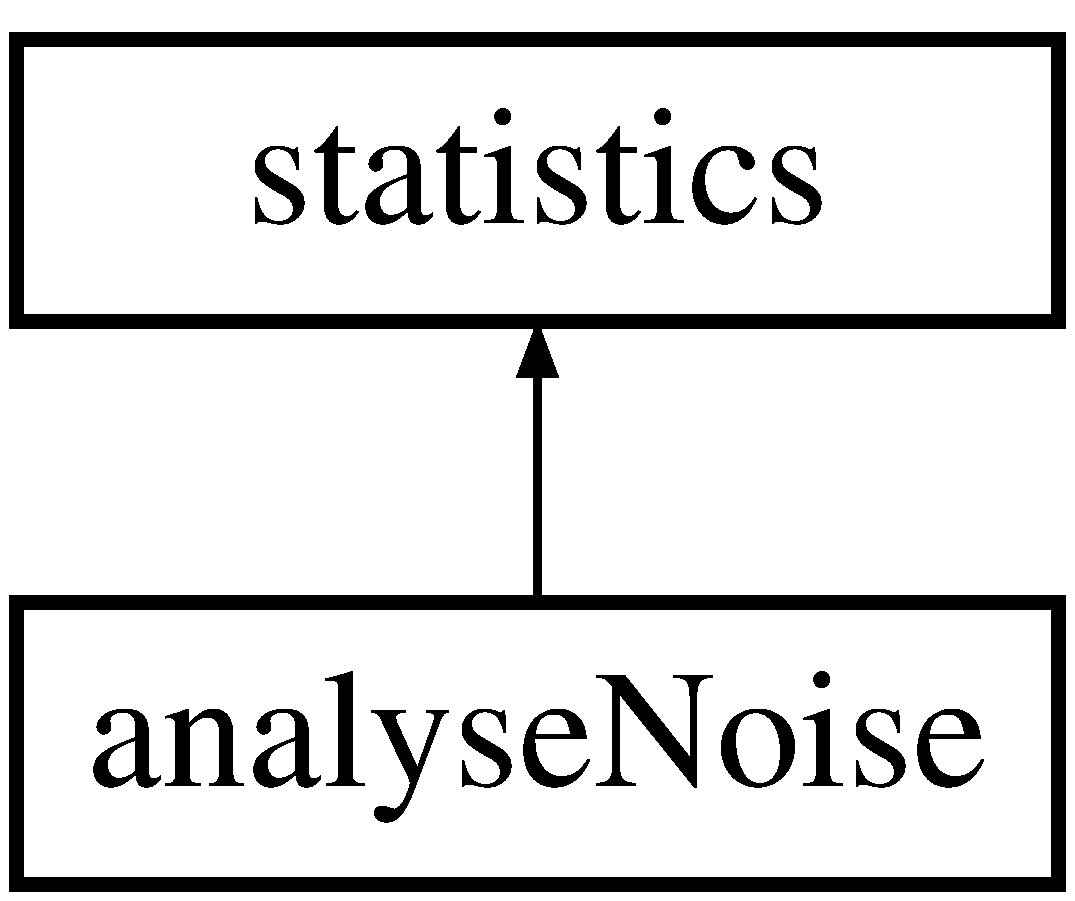
\includegraphics[height=2.000000cm]{classanalyseNoise}
\end{center}
\end{figure}
\subsection*{Public Member Functions}
\begin{DoxyCompactItemize}
\item 
\hyperlink{classanalyseNoise_a3aa97ee9192d62ed488b8942ef0b8acf}{analyse\-Noise} ()
\item 
\hyperlink{classanalyseNoise_ac9f74d3e07f31186904ad86593c8795f}{$\sim$analyse\-Noise} ()
\item 
void \hyperlink{classanalyseNoise_a0daed443334defb0b7262457cb7d7176}{of} (unsigned short $\ast$data, int n, int seg, int skip)
\end{DoxyCompactItemize}
\subsection*{Additional Inherited Members}


\subsection{Detailed Description}
Analyse the noise level of a given time series. 

\subsection{Constructor \& Destructor Documentation}
\hypertarget{classanalyseNoise_a3aa97ee9192d62ed488b8942ef0b8acf}{\index{analyse\-Noise@{analyse\-Noise}!analyse\-Noise@{analyse\-Noise}}
\index{analyse\-Noise@{analyse\-Noise}!analyseNoise@{analyse\-Noise}}
\subsubsection[{analyse\-Noise}]{\setlength{\rightskip}{0pt plus 5cm}analyse\-Noise\-::analyse\-Noise (
\begin{DoxyParamCaption}
{}
\end{DoxyParamCaption}
)}}\label{classanalyseNoise_a3aa97ee9192d62ed488b8942ef0b8acf}
\hypertarget{classanalyseNoise_ac9f74d3e07f31186904ad86593c8795f}{\index{analyse\-Noise@{analyse\-Noise}!$\sim$analyse\-Noise@{$\sim$analyse\-Noise}}
\index{$\sim$analyse\-Noise@{$\sim$analyse\-Noise}!analyseNoise@{analyse\-Noise}}
\subsubsection[{$\sim$analyse\-Noise}]{\setlength{\rightskip}{0pt plus 5cm}analyse\-Noise\-::$\sim$analyse\-Noise (
\begin{DoxyParamCaption}
{}
\end{DoxyParamCaption}
)}}\label{classanalyseNoise_ac9f74d3e07f31186904ad86593c8795f}


\subsection{Member Function Documentation}
\hypertarget{classanalyseNoise_a0daed443334defb0b7262457cb7d7176}{\index{analyse\-Noise@{analyse\-Noise}!of@{of}}
\index{of@{of}!analyseNoise@{analyse\-Noise}}
\subsubsection[{of}]{\setlength{\rightskip}{0pt plus 5cm}void analyse\-Noise\-::of (
\begin{DoxyParamCaption}
\item[{unsigned short $\ast$}]{data, }
\item[{int}]{n, }
\item[{int}]{seg, }
\item[{int}]{skip}
\end{DoxyParamCaption}
)}}\label{classanalyseNoise_a0daed443334defb0b7262457cb7d7176}
Analyse the noise level of a given time series. The alogrithm divides the series in segments. The segments with the highest variance are not consider for the estimation of the noise level parameters. 
\begin{DoxyParams}{Parameters}
{\em data} & Pointer to the time series \\
\hline
{\em n} & Length of the time series \\
\hline
{\em seg} & Length of the segements \\
\hline
{\em skip} & Number of segments to leave out \\
\hline
\end{DoxyParams}


The documentation for this class was generated from the following files\-:\begin{DoxyCompactItemize}
\item 
/home/ntj/\-Development/phd/kitcube-\/tools/src/akutil/\hyperlink{analyseNoise_8h}{analyse\-Noise.\-h}\item 
/home/ntj/\-Development/phd/kitcube-\/tools/src/akutil/\hyperlink{analyseNoise_8cpp}{analyse\-Noise.\-cpp}\end{DoxyCompactItemize}

\hypertarget{classanalysePulse}{\section{analyse\-Pulse Class Reference}
\label{classanalysePulse}\index{analyse\-Pulse@{analyse\-Pulse}}
}


{\ttfamily \#include $<$analyse\-Pulse.\-h$>$}

\subsection*{Public Member Functions}
\begin{DoxyCompactItemize}
\item 
\hyperlink{classanalysePulse_a1bf652998a16d82e894e2a3f84c8d915}{analyse\-Pulse} ()
\item 
\hyperlink{classanalysePulse_ab0fa6bcbb1a94a94181fbffd1337735d}{$\sim$analyse\-Pulse} ()
\item 
void \hyperlink{classanalysePulse_a55294518533cc48e1fb4f3d75e83b1a9}{of} (unsigned short $\ast$data, int n, \hyperlink{classstatistics}{statistics} $\ast$noise)
\item 
int \hyperlink{classanalysePulse_a47d679dc1217690d20831a01ee0b8f58}{calc\-Width} (unsigned short $\ast$data, int n, float tresh)
\item 
unsigned long \hyperlink{classanalysePulse_a8a0f16ccc6afb387fd8f1642a90124a7}{calc\-Charge} (unsigned short $\ast$data, int n, float tresh, unsigned short \hyperlink{classanalysePulse_a9f10e08873da12460e9df17c2052bb7f}{pedestal})
\end{DoxyCompactItemize}
\subsection*{Public Attributes}
\begin{DoxyCompactItemize}
\item 
int \hyperlink{classanalysePulse_a221394fcd9acca79d2239e0303f5fddb}{width}
\item 
unsigned long \hyperlink{classanalysePulse_a627c195d98e2a9df7329eceddb1f9b8a}{charge}
\item 
float \hyperlink{classanalysePulse_a6770c0e1c7f266f52f9ca2bb9f60e78f}{thresh\-W}
\item 
float \hyperlink{classanalysePulse_a13a79360ba44937070cdabeeed8d9a30}{thresh\-C}
\item 
unsigned short \hyperlink{classanalysePulse_a9f10e08873da12460e9df17c2052bb7f}{pedestal}
\end{DoxyCompactItemize}


\subsection{Detailed Description}
Analyse the properties of a pulse in a given time series. 

\subsection{Constructor \& Destructor Documentation}
\hypertarget{classanalysePulse_a1bf652998a16d82e894e2a3f84c8d915}{\index{analyse\-Pulse@{analyse\-Pulse}!analyse\-Pulse@{analyse\-Pulse}}
\index{analyse\-Pulse@{analyse\-Pulse}!analysePulse@{analyse\-Pulse}}
\subsubsection[{analyse\-Pulse}]{\setlength{\rightskip}{0pt plus 5cm}analyse\-Pulse\-::analyse\-Pulse (
\begin{DoxyParamCaption}
{}
\end{DoxyParamCaption}
)}}\label{classanalysePulse_a1bf652998a16d82e894e2a3f84c8d915}
\hypertarget{classanalysePulse_ab0fa6bcbb1a94a94181fbffd1337735d}{\index{analyse\-Pulse@{analyse\-Pulse}!$\sim$analyse\-Pulse@{$\sim$analyse\-Pulse}}
\index{$\sim$analyse\-Pulse@{$\sim$analyse\-Pulse}!analysePulse@{analyse\-Pulse}}
\subsubsection[{$\sim$analyse\-Pulse}]{\setlength{\rightskip}{0pt plus 5cm}analyse\-Pulse\-::$\sim$analyse\-Pulse (
\begin{DoxyParamCaption}
{}
\end{DoxyParamCaption}
)}}\label{classanalysePulse_ab0fa6bcbb1a94a94181fbffd1337735d}


\subsection{Member Function Documentation}
\hypertarget{classanalysePulse_a8a0f16ccc6afb387fd8f1642a90124a7}{\index{analyse\-Pulse@{analyse\-Pulse}!calc\-Charge@{calc\-Charge}}
\index{calc\-Charge@{calc\-Charge}!analysePulse@{analyse\-Pulse}}
\subsubsection[{calc\-Charge}]{\setlength{\rightskip}{0pt plus 5cm}unsigned long analyse\-Pulse\-::calc\-Charge (
\begin{DoxyParamCaption}
\item[{unsigned short $\ast$}]{data, }
\item[{int}]{n, }
\item[{float}]{tresh, }
\item[{unsigned short}]{pedestal}
\end{DoxyParamCaption}
)}}\label{classanalysePulse_a8a0f16ccc6afb387fd8f1642a90124a7}
\hypertarget{classanalysePulse_a47d679dc1217690d20831a01ee0b8f58}{\index{analyse\-Pulse@{analyse\-Pulse}!calc\-Width@{calc\-Width}}
\index{calc\-Width@{calc\-Width}!analysePulse@{analyse\-Pulse}}
\subsubsection[{calc\-Width}]{\setlength{\rightskip}{0pt plus 5cm}int analyse\-Pulse\-::calc\-Width (
\begin{DoxyParamCaption}
\item[{unsigned short $\ast$}]{data, }
\item[{int}]{n, }
\item[{float}]{tresh}
\end{DoxyParamCaption}
)}}\label{classanalysePulse_a47d679dc1217690d20831a01ee0b8f58}
\hypertarget{classanalysePulse_a55294518533cc48e1fb4f3d75e83b1a9}{\index{analyse\-Pulse@{analyse\-Pulse}!of@{of}}
\index{of@{of}!analysePulse@{analyse\-Pulse}}
\subsubsection[{of}]{\setlength{\rightskip}{0pt plus 5cm}void analyse\-Pulse\-::of (
\begin{DoxyParamCaption}
\item[{unsigned short $\ast$}]{data, }
\item[{int}]{n, }
\item[{{\bf statistics} $\ast$}]{noise}
\end{DoxyParamCaption}
)}}\label{classanalysePulse_a55294518533cc48e1fb4f3d75e83b1a9}


\subsection{Member Data Documentation}
\hypertarget{classanalysePulse_a627c195d98e2a9df7329eceddb1f9b8a}{\index{analyse\-Pulse@{analyse\-Pulse}!charge@{charge}}
\index{charge@{charge}!analysePulse@{analyse\-Pulse}}
\subsubsection[{charge}]{\setlength{\rightskip}{0pt plus 5cm}unsigned long analyse\-Pulse\-::charge}}\label{classanalysePulse_a627c195d98e2a9df7329eceddb1f9b8a}
\hypertarget{classanalysePulse_a9f10e08873da12460e9df17c2052bb7f}{\index{analyse\-Pulse@{analyse\-Pulse}!pedestal@{pedestal}}
\index{pedestal@{pedestal}!analysePulse@{analyse\-Pulse}}
\subsubsection[{pedestal}]{\setlength{\rightskip}{0pt plus 5cm}unsigned short analyse\-Pulse\-::pedestal}}\label{classanalysePulse_a9f10e08873da12460e9df17c2052bb7f}
\hypertarget{classanalysePulse_a13a79360ba44937070cdabeeed8d9a30}{\index{analyse\-Pulse@{analyse\-Pulse}!thresh\-C@{thresh\-C}}
\index{thresh\-C@{thresh\-C}!analysePulse@{analyse\-Pulse}}
\subsubsection[{thresh\-C}]{\setlength{\rightskip}{0pt plus 5cm}float analyse\-Pulse\-::thresh\-C}}\label{classanalysePulse_a13a79360ba44937070cdabeeed8d9a30}
\hypertarget{classanalysePulse_a6770c0e1c7f266f52f9ca2bb9f60e78f}{\index{analyse\-Pulse@{analyse\-Pulse}!thresh\-W@{thresh\-W}}
\index{thresh\-W@{thresh\-W}!analysePulse@{analyse\-Pulse}}
\subsubsection[{thresh\-W}]{\setlength{\rightskip}{0pt plus 5cm}float analyse\-Pulse\-::thresh\-W}}\label{classanalysePulse_a6770c0e1c7f266f52f9ca2bb9f60e78f}
\hypertarget{classanalysePulse_a221394fcd9acca79d2239e0303f5fddb}{\index{analyse\-Pulse@{analyse\-Pulse}!width@{width}}
\index{width@{width}!analysePulse@{analyse\-Pulse}}
\subsubsection[{width}]{\setlength{\rightskip}{0pt plus 5cm}int analyse\-Pulse\-::width}}\label{classanalysePulse_a221394fcd9acca79d2239e0303f5fddb}


The documentation for this class was generated from the following files\-:\begin{DoxyCompactItemize}
\item 
/home/ntj/\-Development/phd/kitcube-\/tools/src/akutil/\hyperlink{analysePulse_8h}{analyse\-Pulse.\-h}\item 
/home/ntj/\-Development/phd/kitcube-\/tools/src/akutil/\hyperlink{analysePulse_8cpp}{analyse\-Pulse.\-cpp}\end{DoxyCompactItemize}

\hypertarget{structaxisDef}{\section{axis\-Def Struct Reference}
\label{structaxisDef}\index{axis\-Def@{axis\-Def}}
}


{\ttfamily \#include $<$daqdevice.\-h$>$}

\subsection*{Public Attributes}
\begin{DoxyCompactItemize}
\item 
std\-::string \hyperlink{structaxisDef_aad90dd24f442707e3c5cbc9a63ace2ac}{name}
\item 
std\-::string \hyperlink{structaxisDef_a2cb1c26f0d063ce888d83393c672d6d3}{desc}
\item 
std\-::string \hyperlink{structaxisDef_a5400e43536c69ae82dac0645699415fc}{unit}
\item 
float \hyperlink{structaxisDef_a82d8f9c129ca390eb253d2231ce6b8f3}{range\-Min}
\item 
float \hyperlink{structaxisDef_ae5b71d00e16d1270d602eaedd2e5ec88}{range\-Max}
\item 
bool \hyperlink{structaxisDef_aea953fb050c60d7260882239ca0672f2}{is\-New}
\item 
int \hyperlink{structaxisDef_a1d36c9abefe4d6788f325ebc5278a8e8}{id}
\end{DoxyCompactItemize}


\subsection{Member Data Documentation}
\hypertarget{structaxisDef_a2cb1c26f0d063ce888d83393c672d6d3}{\index{axis\-Def@{axis\-Def}!desc@{desc}}
\index{desc@{desc}!axisDef@{axis\-Def}}
\subsubsection[{desc}]{\setlength{\rightskip}{0pt plus 5cm}std\-::string axis\-Def\-::desc}}\label{structaxisDef_a2cb1c26f0d063ce888d83393c672d6d3}
\hypertarget{structaxisDef_a1d36c9abefe4d6788f325ebc5278a8e8}{\index{axis\-Def@{axis\-Def}!id@{id}}
\index{id@{id}!axisDef@{axis\-Def}}
\subsubsection[{id}]{\setlength{\rightskip}{0pt plus 5cm}int axis\-Def\-::id}}\label{structaxisDef_a1d36c9abefe4d6788f325ebc5278a8e8}
\hypertarget{structaxisDef_aea953fb050c60d7260882239ca0672f2}{\index{axis\-Def@{axis\-Def}!is\-New@{is\-New}}
\index{is\-New@{is\-New}!axisDef@{axis\-Def}}
\subsubsection[{is\-New}]{\setlength{\rightskip}{0pt plus 5cm}bool axis\-Def\-::is\-New}}\label{structaxisDef_aea953fb050c60d7260882239ca0672f2}
\hypertarget{structaxisDef_aad90dd24f442707e3c5cbc9a63ace2ac}{\index{axis\-Def@{axis\-Def}!name@{name}}
\index{name@{name}!axisDef@{axis\-Def}}
\subsubsection[{name}]{\setlength{\rightskip}{0pt plus 5cm}std\-::string axis\-Def\-::name}}\label{structaxisDef_aad90dd24f442707e3c5cbc9a63ace2ac}
\hypertarget{structaxisDef_ae5b71d00e16d1270d602eaedd2e5ec88}{\index{axis\-Def@{axis\-Def}!range\-Max@{range\-Max}}
\index{range\-Max@{range\-Max}!axisDef@{axis\-Def}}
\subsubsection[{range\-Max}]{\setlength{\rightskip}{0pt plus 5cm}float axis\-Def\-::range\-Max}}\label{structaxisDef_ae5b71d00e16d1270d602eaedd2e5ec88}
\hypertarget{structaxisDef_a82d8f9c129ca390eb253d2231ce6b8f3}{\index{axis\-Def@{axis\-Def}!range\-Min@{range\-Min}}
\index{range\-Min@{range\-Min}!axisDef@{axis\-Def}}
\subsubsection[{range\-Min}]{\setlength{\rightskip}{0pt plus 5cm}float axis\-Def\-::range\-Min}}\label{structaxisDef_a82d8f9c129ca390eb253d2231ce6b8f3}
\hypertarget{structaxisDef_a5400e43536c69ae82dac0645699415fc}{\index{axis\-Def@{axis\-Def}!unit@{unit}}
\index{unit@{unit}!axisDef@{axis\-Def}}
\subsubsection[{unit}]{\setlength{\rightskip}{0pt plus 5cm}std\-::string axis\-Def\-::unit}}\label{structaxisDef_a5400e43536c69ae82dac0645699415fc}


The documentation for this struct was generated from the following file\-:\begin{DoxyCompactItemize}
\item 
/home/ntj/\-Development/phd/kitcube-\/tools/src/kitcube-\/devices/\hyperlink{daqdevice_8h}{daqdevice.\-h}\end{DoxyCompactItemize}

\hypertarget{classBaseServer}{\section{Base\-Server Class Reference}
\label{classBaseServer}\index{Base\-Server@{Base\-Server}}
}


{\ttfamily \#include $<$baseserver.\-h$>$}

Inheritance diagram for Base\-Server\-:\begin{figure}[H]
\begin{center}
\leavevmode
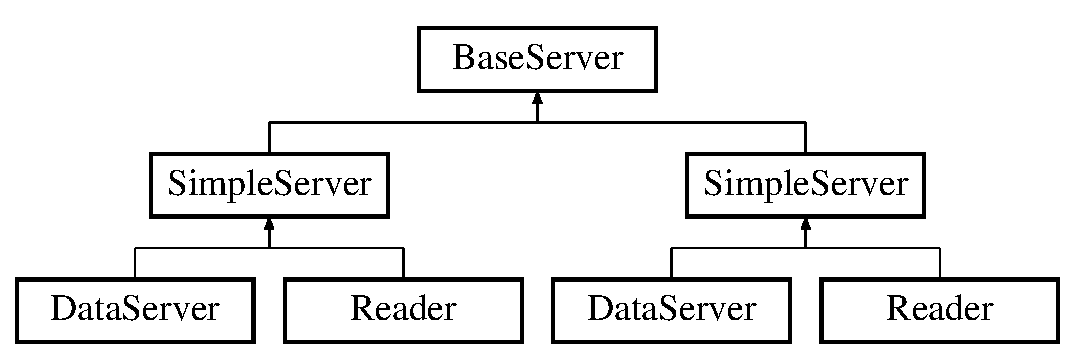
\includegraphics[height=3.000000cm]{classBaseServer}
\end{center}
\end{figure}
\subsection*{Public Member Functions}
\begin{DoxyCompactItemize}
\item 
\hyperlink{classBaseServer_a04931ee29456204b3ef3eb8f7d496f3b}{Base\-Server} (unsigned short \hyperlink{classBaseServer_a66052c095234e31cada29b678b039c68}{port})
\item 
virtual \hyperlink{classBaseServer_af26a04f6b9e4a614157bf92b69765979}{$\sim$\-Base\-Server} ()
\item 
void \hyperlink{classBaseServer_aa62de94b6fdf829df0cffe05db5f6120}{set\-Debug\-Level} (int \hyperlink{classBaseServer_a078ea2911e24a247cfec950e13bb78dc}{debug})
\item 
void \hyperlink{classBaseServer_a8718ce2924a44417b363901df8c23eb3}{set\-Connection\-Logging} (bool logging=true)
\item 
int \hyperlink{classBaseServer_afde0942ae323e3a4b3e748d227b24c55}{read\-Msg} (int client, char $\ast$msg, int n)
\item 
int \hyperlink{classBaseServer_a1841f7210f1e7083320d2c5c43a238d1}{write\-Msg} (int client, char $\ast$msg, int n=0)
\item 
int \hyperlink{classBaseServer_afdbd104f5be856c7c58426cacfeda1d1}{read\-Data} (int client, unsigned long $\ast$data, int n)
\item 
int \hyperlink{classBaseServer_adf88b5234a4f4d8b628532d8c6414411}{write\-Data} (int client, unsigned long $\ast$data, int n)
\item 
int \hyperlink{classBaseServer_aa0d062a605ff448863f34289da258cfd}{read\-Data} (int client, unsigned int $\ast$data, int n)
\item 
int \hyperlink{classBaseServer_a8273745a09b80f9ab45dabdef43b783d}{write\-Data} (int client, unsigned int $\ast$data, int n)
\item 
int \hyperlink{classBaseServer_aa904ae62925129a82c11845ddda25aa2}{read\-Packet} (int client, unsigned long $\ast$data, int max)
\item 
int \hyperlink{classBaseServer_a93e4a6401e0b0937116feb9af915f2b0}{write\-Packet} (int client, unsigned long $\ast$data, int n)
\item 
void \hyperlink{classBaseServer_ac4ca7f212bdcba0d1fe485bc74f3010b}{monitor} ()
\item 
void \hyperlink{classBaseServer_aef1fa86f254fcb22d1c70541f32adca1}{display} ()
\item 
virtual void \hyperlink{classBaseServer_ad624f5b571be84795564f5591b935447}{show} ()
\item 
void \hyperlink{classBaseServer_a24c84f0313d09d3a3585b3dcaf7dccd9}{init} (F\-I\-L\-E $\ast$\hyperlink{classBaseServer_a9ad43261a042fbeeafee33ca4c0b3fd3}{fout}=stdout)
\item 
void \hyperlink{classBaseServer_aab359a913d5494d783178c7887f0e3ef}{init\-\_\-server} (int fd1=-\/1, int fd2=-\/1)
\item 
void \hyperlink{classBaseServer_a377c95f40422ee8c80f8344a0e90cb3a}{kill\-\_\-server} ()
\item 
void \hyperlink{classBaseServer_ae3172b36c67a4cfd5eac9770f9ea8172}{display\-Active\-Sockets} ()
\item 
void \hyperlink{classBaseServer_ae06367103d97f105e8cbb97ee81c8b83}{display\-Active\-Sockets} (F\-I\-L\-E $\ast$\hyperlink{classBaseServer_a9ad43261a042fbeeafee33ca4c0b3fd3}{fout})
\item 
void \hyperlink{classBaseServer_abfda17e7318193d8fc397f2bc67b6d0b}{set\-T\-Ref} (struct timeval $\ast$time)
\item 
void \hyperlink{classBaseServer_a61ab16b5f61c3f28e75ed57c2f56110e}{enable\-Timeout} (struct timeval $\ast$timeout=0)
\item 
void \hyperlink{classBaseServer_aff06d769604bc32179ea3adb54ccaefc}{disable\-Timeout} ()
\item 
\hyperlink{classBaseServer_a04931ee29456204b3ef3eb8f7d496f3b}{Base\-Server} (unsigned short \hyperlink{classBaseServer_a66052c095234e31cada29b678b039c68}{port})
\item 
virtual \hyperlink{classBaseServer_a5aa74bf7b8d3f41b9002107b03a91977}{$\sim$\-Base\-Server} ()
\item 
void \hyperlink{classBaseServer_aa62de94b6fdf829df0cffe05db5f6120}{set\-Debug\-Level} (int \hyperlink{classBaseServer_a078ea2911e24a247cfec950e13bb78dc}{debug})
\item 
void \hyperlink{classBaseServer_a8718ce2924a44417b363901df8c23eb3}{set\-Connection\-Logging} (bool logging=true)
\item 
int \hyperlink{classBaseServer_afde0942ae323e3a4b3e748d227b24c55}{read\-Msg} (int client, char $\ast$msg, int n)
\item 
int \hyperlink{classBaseServer_a1841f7210f1e7083320d2c5c43a238d1}{write\-Msg} (int client, char $\ast$msg, int n=0)
\item 
int \hyperlink{classBaseServer_afdbd104f5be856c7c58426cacfeda1d1}{read\-Data} (int client, unsigned long $\ast$data, int n)
\item 
int \hyperlink{classBaseServer_adf88b5234a4f4d8b628532d8c6414411}{write\-Data} (int client, unsigned long $\ast$data, int n)
\item 
int \hyperlink{classBaseServer_aa0d062a605ff448863f34289da258cfd}{read\-Data} (int client, unsigned int $\ast$data, int n)
\item 
int \hyperlink{classBaseServer_a8273745a09b80f9ab45dabdef43b783d}{write\-Data} (int client, unsigned int $\ast$data, int n)
\item 
int \hyperlink{classBaseServer_aa904ae62925129a82c11845ddda25aa2}{read\-Packet} (int client, unsigned long $\ast$data, int max)
\item 
int \hyperlink{classBaseServer_a93e4a6401e0b0937116feb9af915f2b0}{write\-Packet} (int client, unsigned long $\ast$data, int n)
\item 
void \hyperlink{classBaseServer_ac4ca7f212bdcba0d1fe485bc74f3010b}{monitor} ()
\item 
void \hyperlink{classBaseServer_aef1fa86f254fcb22d1c70541f32adca1}{display} ()
\item 
virtual void \hyperlink{classBaseServer_a80e40ca3d4c622aa85f199fe43b8803d}{show} ()
\item 
void \hyperlink{classBaseServer_a24c84f0313d09d3a3585b3dcaf7dccd9}{init} (F\-I\-L\-E $\ast$\hyperlink{classBaseServer_a9ad43261a042fbeeafee33ca4c0b3fd3}{fout}=stdout)
\item 
void \hyperlink{classBaseServer_aab359a913d5494d783178c7887f0e3ef}{init\-\_\-server} (int fd1=-\/1, int fd2=-\/1)
\item 
void \hyperlink{classBaseServer_a377c95f40422ee8c80f8344a0e90cb3a}{kill\-\_\-server} ()
\item 
void \hyperlink{classBaseServer_ae3172b36c67a4cfd5eac9770f9ea8172}{display\-Active\-Sockets} ()
\item 
void \hyperlink{classBaseServer_ae06367103d97f105e8cbb97ee81c8b83}{display\-Active\-Sockets} (F\-I\-L\-E $\ast$\hyperlink{classBaseServer_a9ad43261a042fbeeafee33ca4c0b3fd3}{fout})
\item 
void \hyperlink{classBaseServer_abfda17e7318193d8fc397f2bc67b6d0b}{set\-T\-Ref} (struct timeval $\ast$time)
\item 
void \hyperlink{classBaseServer_a61ab16b5f61c3f28e75ed57c2f56110e}{enable\-Timeout} (struct timeval $\ast$timeout=0)
\item 
void \hyperlink{classBaseServer_aff06d769604bc32179ea3adb54ccaefc}{disable\-Timeout} ()
\end{DoxyCompactItemize}
\subsection*{Protected Member Functions}
\begin{DoxyCompactItemize}
\item 
void \hyperlink{classBaseServer_a6f8a3014ddd5175bcd8f6693b5dc5920}{set\-Port} (unsigned short \hyperlink{classBaseServer_a66052c095234e31cada29b678b039c68}{port})
\item 
virtual int \hyperlink{classBaseServer_a892cf59b889f59d73031108cfab07772}{handle\-\_\-timeout} ()
\item 
void \hyperlink{classBaseServer_a7144e0d3ba2ea07df19aaa45eee2f88d}{get\-Next\-Timeout} (int $\ast$i\-Sample, struct timeval $\ast$timeout)
\item 
void \hyperlink{classBaseServer_a3b0303f1db9d43aa3fcbb5ff3b1fac00}{display\-Msg} (unsigned char $\ast$msg, int len)
\item 
virtual int \hyperlink{classBaseServer_a3e649e1a9564008b2728b429bcb7e192}{read\-\_\-from\-\_\-client} (int filedes)
\item 
virtual int \hyperlink{classBaseServer_a2c5a73b3bd9950a7809ac2a353061960}{read\-\_\-from\-\_\-keyboard} ()
\item 
virtual void \hyperlink{classBaseServer_a4dade2ab6b6f0c1b1030afe1cca16af0}{display\-Version} ()
\item 
void \hyperlink{classBaseServer_a3277d0713a661a87bb64a42e7f7f9adc}{endian\-\_\-swap} (unsigned short \&x)
\item 
void \hyperlink{classBaseServer_a1f74086ad80ccab0d132b9e6ae026931}{endian\-\_\-swap} (uint32\-\_\-t \&x)
\item 
void \hyperlink{classBaseServer_a80490b4fe26e45a7de5f500af59a43e2}{endian\-\_\-swap} (unsigned long \&x)
\item 
void \hyperlink{classBaseServer_afb5c1352240c2db41febc6a666881ae3}{endian\-\_\-swap} (unsigned long long \&x)
\item 
void \hyperlink{classBaseServer_a97d6e2df8169b3f8da02099626612848}{endian\-\_\-prepare\-\_\-string} (unsigned long \&x)
\item 
void \hyperlink{classBaseServer_af4c5ce4338acc13dcf5d6e4829ba27dc}{endian\-\_\-prepare\-\_\-short} (unsigned long \&x)
\item 
void \hyperlink{classBaseServer_a6628b9fe3bc35e7814ddc2b68564c4aa}{endian\-\_\-swap} (double \&x)
\item 
void \hyperlink{classBaseServer_a6f8a3014ddd5175bcd8f6693b5dc5920}{set\-Port} (unsigned short \hyperlink{classBaseServer_a66052c095234e31cada29b678b039c68}{port})
\item 
virtual int \hyperlink{classBaseServer_abf4522aaa35b5d912f52e0fa37ebac7f}{handle\-\_\-timeout} ()
\item 
void \hyperlink{classBaseServer_a7144e0d3ba2ea07df19aaa45eee2f88d}{get\-Next\-Timeout} (int $\ast$i\-Sample, struct timeval $\ast$timeout)
\item 
void \hyperlink{classBaseServer_a3b0303f1db9d43aa3fcbb5ff3b1fac00}{display\-Msg} (unsigned char $\ast$msg, int len)
\item 
virtual int \hyperlink{classBaseServer_a113ea8f8a7513c5de594c7450c15f88e}{read\-\_\-from\-\_\-client} (int filedes)
\item 
virtual int \hyperlink{classBaseServer_adcd355f20c31da752d9c96d70ab44533}{read\-\_\-from\-\_\-keyboard} ()
\item 
virtual void \hyperlink{classBaseServer_a138c082fc43509f250ffd34e1748335b}{display\-Version} ()
\item 
void \hyperlink{classBaseServer_a3277d0713a661a87bb64a42e7f7f9adc}{endian\-\_\-swap} (unsigned short \&x)
\item 
void \hyperlink{classBaseServer_a1f74086ad80ccab0d132b9e6ae026931}{endian\-\_\-swap} (uint32\-\_\-t \&x)
\item 
void \hyperlink{classBaseServer_a80490b4fe26e45a7de5f500af59a43e2}{endian\-\_\-swap} (unsigned long \&x)
\item 
void \hyperlink{classBaseServer_afb5c1352240c2db41febc6a666881ae3}{endian\-\_\-swap} (unsigned long long \&x)
\item 
void \hyperlink{classBaseServer_a97d6e2df8169b3f8da02099626612848}{endian\-\_\-prepare\-\_\-string} (unsigned long \&x)
\item 
void \hyperlink{classBaseServer_af4c5ce4338acc13dcf5d6e4829ba27dc}{endian\-\_\-prepare\-\_\-short} (unsigned long \&x)
\item 
void \hyperlink{classBaseServer_a6628b9fe3bc35e7814ddc2b68564c4aa}{endian\-\_\-swap} (double \&x)
\end{DoxyCompactItemize}
\subsection*{Protected Attributes}
\begin{DoxyCompactItemize}
\item 
int \hyperlink{classBaseServer_a078ea2911e24a247cfec950e13bb78dc}{debug}
\item 
F\-I\-L\-E $\ast$ \hyperlink{classBaseServer_a9ad43261a042fbeeafee33ca4c0b3fd3}{fout}
\item 
bool \hyperlink{classBaseServer_a7d1dd18825bf1ff1c7c7ec0a8903c340}{shutdown}
\item 
fd\-\_\-set \hyperlink{classBaseServer_a9c66924719c4c28d5088dc6359dcf114}{active\-\_\-fd\-\_\-set}
\item 
fd\-\_\-set \hyperlink{classBaseServer_a3e5463a0e428bacd9a23d8f1e03ed943}{change\-\_\-byteorder\-\_\-fd\-\_\-set}
\item 
unsigned short \hyperlink{classBaseServer_a66052c095234e31cada29b678b039c68}{port}
\item 
S\-O\-C\-K\-E\-T \hyperlink{classBaseServer_a8ab6dde541feb79b2315a4fb96918ce6}{sock}
\item 
struct timeval \hyperlink{classBaseServer_a577aa72c0ceda0fb61ae1ebdaca46540}{t\-Ref}
\item 
struct timezone \hyperlink{classBaseServer_a234e5bf97bfbddb110ca8505d16e1ca0}{t\-Zone}
\item 
struct timeval \hyperlink{classBaseServer_a033ccd3b1b9218b8df7c5bac0f16b08e}{t\-Sample}
\item 
int \hyperlink{classBaseServer_a19c0599639c04521eef256b0c3215c5f}{index}
\item 
int \hyperlink{classBaseServer_aa62931fdc3513ffb3e39efb1f1a412b5}{n\-Samples}
\item 
int \hyperlink{classBaseServer_ae6bf1d5aaa70401472f0a355887ab007}{last\-Index}
\item 
struct timeval \hyperlink{classBaseServer_acd804e8f5dbbf12372661674e9efd4a5}{ttimer}
\item 
bool \hyperlink{classBaseServer_a68765146a8e39ba997e3e08ecb23634c}{use\-Timeout}
\item 
bool \hyperlink{classBaseServer_a59d77b9f67ebe2249d592360ba0ebee2}{conn\-Logging}
\end{DoxyCompactItemize}


\subsection{Detailed Description}
Implements a simple I\-P server.

The server waits for connections. The communication with the client is defined in the protected function read\-\_\-from\-\_\-client. Overload this function for a specific application.

The server allows to communicate with clients that use different bytes order. The list change\-\_\-byteorder\-\_\-fd\-\_\-set contains all connections that do not operate with the same byte order. The server always tries to communicate with it's own native byte order. The protocoll does not exchange all data in network byte order. (Compile flag U\-S\-E\-\_\-\-D\-Y\-N\-\_\-\-B\-Y\-T\-E\-O\-R\-E\-R). The disabled compile flag U\-S\-E\-\_\-\-B\-Y\-T\-E\-O\-R\-D\-E\-R transvers all variables in network byte order.

\begin{DoxyRefDesc}{Todo}
\item[\hyperlink{todo__todo000001}{Todo}]Use a independant threads for all connections. If one connection hangs, the other won't be affected?! 

Improve the Server managment. Loging, Shutdown via I\-P. For some other purpose a New class similar to Pbus/\-Pbus\-Proxy couble may be useful for maintenance and run control. Eg. shutdown + restart of the Server, Control of the I\-Rdispatcher!!!\end{DoxyRefDesc}


Changes\-: \begin{DoxyItemize}
\item 4.\-11.\-02 ak\-: Add stdin to the select functions. The server is now responding to socket and keyboard input! Improved output of the server -\/ format similar to that of netstat --ip. \item 31.\-10.\-02 ak\-: Closing all connected sockets before shutdown. This prevents hanging connections after terminating the server. \item 18.\-3.\-01 ak\-: Protected variable for the output stream introduced -\/ stop this nasty messages in the terminal!!!\end{DoxyItemize}
Implements a simple I\-P server.

The server waits for connections. The communication with the client is defined in the protected function read\-\_\-from\-\_\-client. Overload this function for a specific application.

The server allows to communicate with clients that use different bytes order. The list change\-\_\-byteorder\-\_\-fd\-\_\-set contains all connections that do not operate with the same byte order. The server always tries to communicate with it's own native byte order. The protocoll does not exchange all data in network byte order. (Compile flag U\-S\-E\-\_\-\-D\-Y\-N\-\_\-\-B\-Y\-T\-E\-O\-R\-E\-R). The disabled compile flag U\-S\-E\-\_\-\-B\-Y\-T\-E\-O\-R\-D\-E\-R transvers all variables in network byte order.

\begin{DoxyRefDesc}{Todo}
\item[\hyperlink{todo__todo000009}{Todo}]Use a independant threads for all connections. If one connection hangs, the other won't be affected?! 

Improve the Server managment. Loging, Shutdown via I\-P. For some other purpose a New class similar to Pbus/\-Pbus\-Proxy couble may be useful for maintenance and run control. Eg. shutdown + restart of the Server, Control of the I\-Rdispatcher!!!\end{DoxyRefDesc}


Changes\-: \begin{DoxyItemize}
\item 4.\-11.\-02 ak\-: Add stdin to the select functions. The server is now responding to socket and keyboard input! Improved output of the server -\/ format similar to that of netstat --ip. \item 31.\-10.\-02 ak\-: Closing all connected sockets before shutdown. This prevents hanging connections after terminating the server. \item 18.\-3.\-01 ak\-: Protected variable for the output stream introduced -\/ stop this nasty messages in the terminal!!! \end{DoxyItemize}


\subsection{Constructor \& Destructor Documentation}
\hypertarget{classBaseServer_a04931ee29456204b3ef3eb8f7d496f3b}{\index{Base\-Server@{Base\-Server}!Base\-Server@{Base\-Server}}
\index{Base\-Server@{Base\-Server}!BaseServer@{Base\-Server}}
\subsubsection[{Base\-Server}]{\setlength{\rightskip}{0pt plus 5cm}Base\-Server\-::\-Base\-Server (
\begin{DoxyParamCaption}
\item[{unsigned short}]{port}
\end{DoxyParamCaption}
)}}\label{classBaseServer_a04931ee29456204b3ef3eb8f7d496f3b}
\hypertarget{classBaseServer_af26a04f6b9e4a614157bf92b69765979}{\index{Base\-Server@{Base\-Server}!$\sim$\-Base\-Server@{$\sim$\-Base\-Server}}
\index{$\sim$\-Base\-Server@{$\sim$\-Base\-Server}!BaseServer@{Base\-Server}}
\subsubsection[{$\sim$\-Base\-Server}]{\setlength{\rightskip}{0pt plus 5cm}Base\-Server\-::$\sim$\-Base\-Server (
\begin{DoxyParamCaption}
{}
\end{DoxyParamCaption}
)\hspace{0.3cm}{\ttfamily [virtual]}}}\label{classBaseServer_af26a04f6b9e4a614157bf92b69765979}
\hypertarget{classBaseServer_a04931ee29456204b3ef3eb8f7d496f3b}{\index{Base\-Server@{Base\-Server}!Base\-Server@{Base\-Server}}
\index{Base\-Server@{Base\-Server}!BaseServer@{Base\-Server}}
\subsubsection[{Base\-Server}]{\setlength{\rightskip}{0pt plus 5cm}Base\-Server\-::\-Base\-Server (
\begin{DoxyParamCaption}
\item[{unsigned short}]{port}
\end{DoxyParamCaption}
)}}\label{classBaseServer_a04931ee29456204b3ef3eb8f7d496f3b}
\hypertarget{classBaseServer_a5aa74bf7b8d3f41b9002107b03a91977}{\index{Base\-Server@{Base\-Server}!$\sim$\-Base\-Server@{$\sim$\-Base\-Server}}
\index{$\sim$\-Base\-Server@{$\sim$\-Base\-Server}!BaseServer@{Base\-Server}}
\subsubsection[{$\sim$\-Base\-Server}]{\setlength{\rightskip}{0pt plus 5cm}virtual Base\-Server\-::$\sim$\-Base\-Server (
\begin{DoxyParamCaption}
{}
\end{DoxyParamCaption}
)\hspace{0.3cm}{\ttfamily [virtual]}}}\label{classBaseServer_a5aa74bf7b8d3f41b9002107b03a91977}


\subsection{Member Function Documentation}
\hypertarget{classBaseServer_aff06d769604bc32179ea3adb54ccaefc}{\index{Base\-Server@{Base\-Server}!disable\-Timeout@{disable\-Timeout}}
\index{disable\-Timeout@{disable\-Timeout}!BaseServer@{Base\-Server}}
\subsubsection[{disable\-Timeout}]{\setlength{\rightskip}{0pt plus 5cm}void Base\-Server\-::disable\-Timeout (
\begin{DoxyParamCaption}
{}
\end{DoxyParamCaption}
)}}\label{classBaseServer_aff06d769604bc32179ea3adb54ccaefc}
\hypertarget{classBaseServer_aff06d769604bc32179ea3adb54ccaefc}{\index{Base\-Server@{Base\-Server}!disable\-Timeout@{disable\-Timeout}}
\index{disable\-Timeout@{disable\-Timeout}!BaseServer@{Base\-Server}}
\subsubsection[{disable\-Timeout}]{\setlength{\rightskip}{0pt plus 5cm}void Base\-Server\-::disable\-Timeout (
\begin{DoxyParamCaption}
{}
\end{DoxyParamCaption}
)}}\label{classBaseServer_aff06d769604bc32179ea3adb54ccaefc}
\hypertarget{classBaseServer_aef1fa86f254fcb22d1c70541f32adca1}{\index{Base\-Server@{Base\-Server}!display@{display}}
\index{display@{display}!BaseServer@{Base\-Server}}
\subsubsection[{display}]{\setlength{\rightskip}{0pt plus 5cm}void Base\-Server\-::display (
\begin{DoxyParamCaption}
{}
\end{DoxyParamCaption}
)}}\label{classBaseServer_aef1fa86f254fcb22d1c70541f32adca1}
\hypertarget{classBaseServer_aef1fa86f254fcb22d1c70541f32adca1}{\index{Base\-Server@{Base\-Server}!display@{display}}
\index{display@{display}!BaseServer@{Base\-Server}}
\subsubsection[{display}]{\setlength{\rightskip}{0pt plus 5cm}void Base\-Server\-::display (
\begin{DoxyParamCaption}
{}
\end{DoxyParamCaption}
)}}\label{classBaseServer_aef1fa86f254fcb22d1c70541f32adca1}
\hypertarget{classBaseServer_ae3172b36c67a4cfd5eac9770f9ea8172}{\index{Base\-Server@{Base\-Server}!display\-Active\-Sockets@{display\-Active\-Sockets}}
\index{display\-Active\-Sockets@{display\-Active\-Sockets}!BaseServer@{Base\-Server}}
\subsubsection[{display\-Active\-Sockets}]{\setlength{\rightskip}{0pt plus 5cm}void Base\-Server\-::display\-Active\-Sockets (
\begin{DoxyParamCaption}
{}
\end{DoxyParamCaption}
)}}\label{classBaseServer_ae3172b36c67a4cfd5eac9770f9ea8172}
Display all active sockets that are served. The display format is somewhat similar to the output of the shell command \char`\"{}netstat -\/-\/ip\char`\"{}. I\-P number and port number of both sides of the connection are show. \hypertarget{classBaseServer_ae3172b36c67a4cfd5eac9770f9ea8172}{\index{Base\-Server@{Base\-Server}!display\-Active\-Sockets@{display\-Active\-Sockets}}
\index{display\-Active\-Sockets@{display\-Active\-Sockets}!BaseServer@{Base\-Server}}
\subsubsection[{display\-Active\-Sockets}]{\setlength{\rightskip}{0pt plus 5cm}void Base\-Server\-::display\-Active\-Sockets (
\begin{DoxyParamCaption}
{}
\end{DoxyParamCaption}
)}}\label{classBaseServer_ae3172b36c67a4cfd5eac9770f9ea8172}
Display all active sockets that are served. The display format is somewhat similar to the output of the shell command \char`\"{}netstat -\/-\/ip\char`\"{}. I\-P number and port number of both sides of the connection are show. \hypertarget{classBaseServer_ae06367103d97f105e8cbb97ee81c8b83}{\index{Base\-Server@{Base\-Server}!display\-Active\-Sockets@{display\-Active\-Sockets}}
\index{display\-Active\-Sockets@{display\-Active\-Sockets}!BaseServer@{Base\-Server}}
\subsubsection[{display\-Active\-Sockets}]{\setlength{\rightskip}{0pt plus 5cm}void Base\-Server\-::display\-Active\-Sockets (
\begin{DoxyParamCaption}
\item[{F\-I\-L\-E $\ast$}]{fout}
\end{DoxyParamCaption}
)}}\label{classBaseServer_ae06367103d97f105e8cbb97ee81c8b83}
Display all active sockets, but use not the standard output stream defined in the initialization. \hypertarget{classBaseServer_ae06367103d97f105e8cbb97ee81c8b83}{\index{Base\-Server@{Base\-Server}!display\-Active\-Sockets@{display\-Active\-Sockets}}
\index{display\-Active\-Sockets@{display\-Active\-Sockets}!BaseServer@{Base\-Server}}
\subsubsection[{display\-Active\-Sockets}]{\setlength{\rightskip}{0pt plus 5cm}void Base\-Server\-::display\-Active\-Sockets (
\begin{DoxyParamCaption}
\item[{F\-I\-L\-E $\ast$}]{fout}
\end{DoxyParamCaption}
)}}\label{classBaseServer_ae06367103d97f105e8cbb97ee81c8b83}
Display all active sockets, but use not the standard output stream defined in the initialization. \hypertarget{classBaseServer_a3b0303f1db9d43aa3fcbb5ff3b1fac00}{\index{Base\-Server@{Base\-Server}!display\-Msg@{display\-Msg}}
\index{display\-Msg@{display\-Msg}!BaseServer@{Base\-Server}}
\subsubsection[{display\-Msg}]{\setlength{\rightskip}{0pt plus 5cm}void Base\-Server\-::display\-Msg (
\begin{DoxyParamCaption}
\item[{unsigned char $\ast$}]{msg, }
\item[{int}]{len}
\end{DoxyParamCaption}
)\hspace{0.3cm}{\ttfamily [protected]}}}\label{classBaseServer_a3b0303f1db9d43aa3fcbb5ff3b1fac00}
Display a message byte by byte in hex format \hypertarget{classBaseServer_a3b0303f1db9d43aa3fcbb5ff3b1fac00}{\index{Base\-Server@{Base\-Server}!display\-Msg@{display\-Msg}}
\index{display\-Msg@{display\-Msg}!BaseServer@{Base\-Server}}
\subsubsection[{display\-Msg}]{\setlength{\rightskip}{0pt plus 5cm}void Base\-Server\-::display\-Msg (
\begin{DoxyParamCaption}
\item[{unsigned char $\ast$}]{msg, }
\item[{int}]{len}
\end{DoxyParamCaption}
)\hspace{0.3cm}{\ttfamily [protected]}}}\label{classBaseServer_a3b0303f1db9d43aa3fcbb5ff3b1fac00}
Display a message byte by byte in hex format \hypertarget{classBaseServer_a4dade2ab6b6f0c1b1030afe1cca16af0}{\index{Base\-Server@{Base\-Server}!display\-Version@{display\-Version}}
\index{display\-Version@{display\-Version}!BaseServer@{Base\-Server}}
\subsubsection[{display\-Version}]{\setlength{\rightskip}{0pt plus 5cm}void Base\-Server\-::display\-Version (
\begin{DoxyParamCaption}
{}
\end{DoxyParamCaption}
)\hspace{0.3cm}{\ttfamily [protected]}, {\ttfamily [virtual]}}}\label{classBaseServer_a4dade2ab6b6f0c1b1030afe1cca16af0}
\hypertarget{classBaseServer_a138c082fc43509f250ffd34e1748335b}{\index{Base\-Server@{Base\-Server}!display\-Version@{display\-Version}}
\index{display\-Version@{display\-Version}!BaseServer@{Base\-Server}}
\subsubsection[{display\-Version}]{\setlength{\rightskip}{0pt plus 5cm}virtual void Base\-Server\-::display\-Version (
\begin{DoxyParamCaption}
{}
\end{DoxyParamCaption}
)\hspace{0.3cm}{\ttfamily [protected]}, {\ttfamily [virtual]}}}\label{classBaseServer_a138c082fc43509f250ffd34e1748335b}
\hypertarget{classBaseServer_a61ab16b5f61c3f28e75ed57c2f56110e}{\index{Base\-Server@{Base\-Server}!enable\-Timeout@{enable\-Timeout}}
\index{enable\-Timeout@{enable\-Timeout}!BaseServer@{Base\-Server}}
\subsubsection[{enable\-Timeout}]{\setlength{\rightskip}{0pt plus 5cm}void Base\-Server\-::enable\-Timeout (
\begin{DoxyParamCaption}
\item[{struct timeval $\ast$}]{timeout = {\ttfamily 0}}
\end{DoxyParamCaption}
)}}\label{classBaseServer_a61ab16b5f61c3f28e75ed57c2f56110e}
Enable period sampling \hypertarget{classBaseServer_a61ab16b5f61c3f28e75ed57c2f56110e}{\index{Base\-Server@{Base\-Server}!enable\-Timeout@{enable\-Timeout}}
\index{enable\-Timeout@{enable\-Timeout}!BaseServer@{Base\-Server}}
\subsubsection[{enable\-Timeout}]{\setlength{\rightskip}{0pt plus 5cm}void Base\-Server\-::enable\-Timeout (
\begin{DoxyParamCaption}
\item[{struct timeval $\ast$}]{timeout = {\ttfamily 0}}
\end{DoxyParamCaption}
)}}\label{classBaseServer_a61ab16b5f61c3f28e75ed57c2f56110e}
Enable period sampling \hypertarget{classBaseServer_af4c5ce4338acc13dcf5d6e4829ba27dc}{\index{Base\-Server@{Base\-Server}!endian\-\_\-prepare\-\_\-short@{endian\-\_\-prepare\-\_\-short}}
\index{endian\-\_\-prepare\-\_\-short@{endian\-\_\-prepare\-\_\-short}!BaseServer@{Base\-Server}}
\subsubsection[{endian\-\_\-prepare\-\_\-short}]{\setlength{\rightskip}{0pt plus 5cm}void Base\-Server\-::endian\-\_\-prepare\-\_\-short (
\begin{DoxyParamCaption}
\item[{unsigned long \&}]{x}
\end{DoxyParamCaption}
)\hspace{0.3cm}{\ttfamily [inline]}, {\ttfamily [protected]}}}\label{classBaseServer_af4c5ce4338acc13dcf5d6e4829ba27dc}
Prepare transmission of short arrays In case of endian swap all short arrays are scrambled. It is necessary to reorder the arrays before transmission.

Note\-: The function will only work if a even number of short values is transmitted. \hypertarget{classBaseServer_af4c5ce4338acc13dcf5d6e4829ba27dc}{\index{Base\-Server@{Base\-Server}!endian\-\_\-prepare\-\_\-short@{endian\-\_\-prepare\-\_\-short}}
\index{endian\-\_\-prepare\-\_\-short@{endian\-\_\-prepare\-\_\-short}!BaseServer@{Base\-Server}}
\subsubsection[{endian\-\_\-prepare\-\_\-short}]{\setlength{\rightskip}{0pt plus 5cm}void Base\-Server\-::endian\-\_\-prepare\-\_\-short (
\begin{DoxyParamCaption}
\item[{unsigned long \&}]{x}
\end{DoxyParamCaption}
)\hspace{0.3cm}{\ttfamily [inline]}, {\ttfamily [protected]}}}\label{classBaseServer_af4c5ce4338acc13dcf5d6e4829ba27dc}
Prepare transmission of short arrays In case of endian swap all short arrays are scrambled. It is necessary to reorder the arrays before transmission.

Note\-: The function will only work if a even number of short values is transmitted. \hypertarget{classBaseServer_a97d6e2df8169b3f8da02099626612848}{\index{Base\-Server@{Base\-Server}!endian\-\_\-prepare\-\_\-string@{endian\-\_\-prepare\-\_\-string}}
\index{endian\-\_\-prepare\-\_\-string@{endian\-\_\-prepare\-\_\-string}!BaseServer@{Base\-Server}}
\subsubsection[{endian\-\_\-prepare\-\_\-string}]{\setlength{\rightskip}{0pt plus 5cm}void Base\-Server\-::endian\-\_\-prepare\-\_\-string (
\begin{DoxyParamCaption}
\item[{unsigned long \&}]{x}
\end{DoxyParamCaption}
)\hspace{0.3cm}{\ttfamily [inline]}, {\ttfamily [protected]}}}\label{classBaseServer_a97d6e2df8169b3f8da02099626612848}
Prepare transmission of character strings In case of endian swap all charcter strings are scrambled. It is necessary to reorder the strings before transmission. \hypertarget{classBaseServer_a97d6e2df8169b3f8da02099626612848}{\index{Base\-Server@{Base\-Server}!endian\-\_\-prepare\-\_\-string@{endian\-\_\-prepare\-\_\-string}}
\index{endian\-\_\-prepare\-\_\-string@{endian\-\_\-prepare\-\_\-string}!BaseServer@{Base\-Server}}
\subsubsection[{endian\-\_\-prepare\-\_\-string}]{\setlength{\rightskip}{0pt plus 5cm}void Base\-Server\-::endian\-\_\-prepare\-\_\-string (
\begin{DoxyParamCaption}
\item[{unsigned long \&}]{x}
\end{DoxyParamCaption}
)\hspace{0.3cm}{\ttfamily [inline]}, {\ttfamily [protected]}}}\label{classBaseServer_a97d6e2df8169b3f8da02099626612848}
Prepare transmission of character strings In case of endian swap all charcter strings are scrambled. It is necessary to reorder the strings before transmission. \hypertarget{classBaseServer_a3277d0713a661a87bb64a42e7f7f9adc}{\index{Base\-Server@{Base\-Server}!endian\-\_\-swap@{endian\-\_\-swap}}
\index{endian\-\_\-swap@{endian\-\_\-swap}!BaseServer@{Base\-Server}}
\subsubsection[{endian\-\_\-swap}]{\setlength{\rightskip}{0pt plus 5cm}void Base\-Server\-::endian\-\_\-swap (
\begin{DoxyParamCaption}
\item[{unsigned short \&}]{x}
\end{DoxyParamCaption}
)\hspace{0.3cm}{\ttfamily [inline]}, {\ttfamily [protected]}}}\label{classBaseServer_a3277d0713a661a87bb64a42e7f7f9adc}
Change byte order of a short variable \hypertarget{classBaseServer_a3277d0713a661a87bb64a42e7f7f9adc}{\index{Base\-Server@{Base\-Server}!endian\-\_\-swap@{endian\-\_\-swap}}
\index{endian\-\_\-swap@{endian\-\_\-swap}!BaseServer@{Base\-Server}}
\subsubsection[{endian\-\_\-swap}]{\setlength{\rightskip}{0pt plus 5cm}void Base\-Server\-::endian\-\_\-swap (
\begin{DoxyParamCaption}
\item[{unsigned short \&}]{x}
\end{DoxyParamCaption}
)\hspace{0.3cm}{\ttfamily [inline]}, {\ttfamily [protected]}}}\label{classBaseServer_a3277d0713a661a87bb64a42e7f7f9adc}
Change byte order of a short variable \hypertarget{classBaseServer_a1f74086ad80ccab0d132b9e6ae026931}{\index{Base\-Server@{Base\-Server}!endian\-\_\-swap@{endian\-\_\-swap}}
\index{endian\-\_\-swap@{endian\-\_\-swap}!BaseServer@{Base\-Server}}
\subsubsection[{endian\-\_\-swap}]{\setlength{\rightskip}{0pt plus 5cm}void Base\-Server\-::endian\-\_\-swap (
\begin{DoxyParamCaption}
\item[{uint32\-\_\-t \&}]{x}
\end{DoxyParamCaption}
)\hspace{0.3cm}{\ttfamily [inline]}, {\ttfamily [protected]}}}\label{classBaseServer_a1f74086ad80ccab0d132b9e6ae026931}
Change byte order of a uint32\-\_\-t variable \hypertarget{classBaseServer_a1f74086ad80ccab0d132b9e6ae026931}{\index{Base\-Server@{Base\-Server}!endian\-\_\-swap@{endian\-\_\-swap}}
\index{endian\-\_\-swap@{endian\-\_\-swap}!BaseServer@{Base\-Server}}
\subsubsection[{endian\-\_\-swap}]{\setlength{\rightskip}{0pt plus 5cm}void Base\-Server\-::endian\-\_\-swap (
\begin{DoxyParamCaption}
\item[{uint32\-\_\-t \&}]{x}
\end{DoxyParamCaption}
)\hspace{0.3cm}{\ttfamily [inline]}, {\ttfamily [protected]}}}\label{classBaseServer_a1f74086ad80ccab0d132b9e6ae026931}
Change byte order of a uint32\-\_\-t variable \hypertarget{classBaseServer_a80490b4fe26e45a7de5f500af59a43e2}{\index{Base\-Server@{Base\-Server}!endian\-\_\-swap@{endian\-\_\-swap}}
\index{endian\-\_\-swap@{endian\-\_\-swap}!BaseServer@{Base\-Server}}
\subsubsection[{endian\-\_\-swap}]{\setlength{\rightskip}{0pt plus 5cm}void Base\-Server\-::endian\-\_\-swap (
\begin{DoxyParamCaption}
\item[{unsigned long \&}]{x}
\end{DoxyParamCaption}
)\hspace{0.3cm}{\ttfamily [inline]}, {\ttfamily [protected]}}}\label{classBaseServer_a80490b4fe26e45a7de5f500af59a43e2}
Change byte order of a long variable \hypertarget{classBaseServer_a80490b4fe26e45a7de5f500af59a43e2}{\index{Base\-Server@{Base\-Server}!endian\-\_\-swap@{endian\-\_\-swap}}
\index{endian\-\_\-swap@{endian\-\_\-swap}!BaseServer@{Base\-Server}}
\subsubsection[{endian\-\_\-swap}]{\setlength{\rightskip}{0pt plus 5cm}void Base\-Server\-::endian\-\_\-swap (
\begin{DoxyParamCaption}
\item[{unsigned long \&}]{x}
\end{DoxyParamCaption}
)\hspace{0.3cm}{\ttfamily [inline]}, {\ttfamily [protected]}}}\label{classBaseServer_a80490b4fe26e45a7de5f500af59a43e2}
Change byte order of a long variable \hypertarget{classBaseServer_afb5c1352240c2db41febc6a666881ae3}{\index{Base\-Server@{Base\-Server}!endian\-\_\-swap@{endian\-\_\-swap}}
\index{endian\-\_\-swap@{endian\-\_\-swap}!BaseServer@{Base\-Server}}
\subsubsection[{endian\-\_\-swap}]{\setlength{\rightskip}{0pt plus 5cm}void Base\-Server\-::endian\-\_\-swap (
\begin{DoxyParamCaption}
\item[{unsigned long long \&}]{x}
\end{DoxyParamCaption}
)\hspace{0.3cm}{\ttfamily [inline]}, {\ttfamily [protected]}}}\label{classBaseServer_afb5c1352240c2db41febc6a666881ae3}
Change byte order for 64bit data types \hypertarget{classBaseServer_afb5c1352240c2db41febc6a666881ae3}{\index{Base\-Server@{Base\-Server}!endian\-\_\-swap@{endian\-\_\-swap}}
\index{endian\-\_\-swap@{endian\-\_\-swap}!BaseServer@{Base\-Server}}
\subsubsection[{endian\-\_\-swap}]{\setlength{\rightskip}{0pt plus 5cm}void Base\-Server\-::endian\-\_\-swap (
\begin{DoxyParamCaption}
\item[{unsigned long long \&}]{x}
\end{DoxyParamCaption}
)\hspace{0.3cm}{\ttfamily [inline]}, {\ttfamily [protected]}}}\label{classBaseServer_afb5c1352240c2db41febc6a666881ae3}
Change byte order for 64bit data types \hypertarget{classBaseServer_a6628b9fe3bc35e7814ddc2b68564c4aa}{\index{Base\-Server@{Base\-Server}!endian\-\_\-swap@{endian\-\_\-swap}}
\index{endian\-\_\-swap@{endian\-\_\-swap}!BaseServer@{Base\-Server}}
\subsubsection[{endian\-\_\-swap}]{\setlength{\rightskip}{0pt plus 5cm}void Base\-Server\-::endian\-\_\-swap (
\begin{DoxyParamCaption}
\item[{double \&}]{x}
\end{DoxyParamCaption}
)\hspace{0.3cm}{\ttfamily [inline]}, {\ttfamily [protected]}}}\label{classBaseServer_a6628b9fe3bc35e7814ddc2b68564c4aa}
\hypertarget{classBaseServer_a6628b9fe3bc35e7814ddc2b68564c4aa}{\index{Base\-Server@{Base\-Server}!endian\-\_\-swap@{endian\-\_\-swap}}
\index{endian\-\_\-swap@{endian\-\_\-swap}!BaseServer@{Base\-Server}}
\subsubsection[{endian\-\_\-swap}]{\setlength{\rightskip}{0pt plus 5cm}void Base\-Server\-::endian\-\_\-swap (
\begin{DoxyParamCaption}
\item[{double \&}]{x}
\end{DoxyParamCaption}
)\hspace{0.3cm}{\ttfamily [inline]}, {\ttfamily [protected]}}}\label{classBaseServer_a6628b9fe3bc35e7814ddc2b68564c4aa}
\hypertarget{classBaseServer_a7144e0d3ba2ea07df19aaa45eee2f88d}{\index{Base\-Server@{Base\-Server}!get\-Next\-Timeout@{get\-Next\-Timeout}}
\index{get\-Next\-Timeout@{get\-Next\-Timeout}!BaseServer@{Base\-Server}}
\subsubsection[{get\-Next\-Timeout}]{\setlength{\rightskip}{0pt plus 5cm}void Base\-Server\-::get\-Next\-Timeout (
\begin{DoxyParamCaption}
\item[{int $\ast$}]{i\-Sample, }
\item[{struct timeval $\ast$}]{timeout}
\end{DoxyParamCaption}
)\hspace{0.3cm}{\ttfamily [protected]}}}\label{classBaseServer_a7144e0d3ba2ea07df19aaa45eee2f88d}
Calculate the time that is left until the next sampling time \hypertarget{classBaseServer_a7144e0d3ba2ea07df19aaa45eee2f88d}{\index{Base\-Server@{Base\-Server}!get\-Next\-Timeout@{get\-Next\-Timeout}}
\index{get\-Next\-Timeout@{get\-Next\-Timeout}!BaseServer@{Base\-Server}}
\subsubsection[{get\-Next\-Timeout}]{\setlength{\rightskip}{0pt plus 5cm}void Base\-Server\-::get\-Next\-Timeout (
\begin{DoxyParamCaption}
\item[{int $\ast$}]{i\-Sample, }
\item[{struct timeval $\ast$}]{timeout}
\end{DoxyParamCaption}
)\hspace{0.3cm}{\ttfamily [protected]}}}\label{classBaseServer_a7144e0d3ba2ea07df19aaa45eee2f88d}
Calculate the time that is left until the next sampling time \hypertarget{classBaseServer_abf4522aaa35b5d912f52e0fa37ebac7f}{\index{Base\-Server@{Base\-Server}!handle\-\_\-timeout@{handle\-\_\-timeout}}
\index{handle\-\_\-timeout@{handle\-\_\-timeout}!BaseServer@{Base\-Server}}
\subsubsection[{handle\-\_\-timeout}]{\setlength{\rightskip}{0pt plus 5cm}virtual int Base\-Server\-::handle\-\_\-timeout (
\begin{DoxyParamCaption}
{}
\end{DoxyParamCaption}
)\hspace{0.3cm}{\ttfamily [protected]}, {\ttfamily [virtual]}}}\label{classBaseServer_abf4522aaa35b5d912f52e0fa37ebac7f}
Do some action after the timeout and before the next select follows 

Reimplemented in \hyperlink{classDataServer_ac45cfcc0fca260f2283bd563281b4efa}{Data\-Server}, and \hyperlink{classReader_a1c23cb1e3ec1a87fb5db65392fb43d21}{Reader}.

\hypertarget{classBaseServer_a892cf59b889f59d73031108cfab07772}{\index{Base\-Server@{Base\-Server}!handle\-\_\-timeout@{handle\-\_\-timeout}}
\index{handle\-\_\-timeout@{handle\-\_\-timeout}!BaseServer@{Base\-Server}}
\subsubsection[{handle\-\_\-timeout}]{\setlength{\rightskip}{0pt plus 5cm}int Base\-Server\-::handle\-\_\-timeout (
\begin{DoxyParamCaption}
{}
\end{DoxyParamCaption}
)\hspace{0.3cm}{\ttfamily [protected]}, {\ttfamily [virtual]}}}\label{classBaseServer_a892cf59b889f59d73031108cfab07772}
Do some action after the timeout and before the next select follows 

Reimplemented in \hyperlink{classDataServer_ac45cfcc0fca260f2283bd563281b4efa}{Data\-Server}, and \hyperlink{classReader_a1c23cb1e3ec1a87fb5db65392fb43d21}{Reader}.

\hypertarget{classBaseServer_a24c84f0313d09d3a3585b3dcaf7dccd9}{\index{Base\-Server@{Base\-Server}!init@{init}}
\index{init@{init}!BaseServer@{Base\-Server}}
\subsubsection[{init}]{\setlength{\rightskip}{0pt plus 5cm}void Base\-Server\-::init (
\begin{DoxyParamCaption}
\item[{F\-I\-L\-E $\ast$}]{fout = {\ttfamily stdout}}
\end{DoxyParamCaption}
)}}\label{classBaseServer_a24c84f0313d09d3a3585b3dcaf7dccd9}
Create the server socket \hypertarget{classBaseServer_a24c84f0313d09d3a3585b3dcaf7dccd9}{\index{Base\-Server@{Base\-Server}!init@{init}}
\index{init@{init}!BaseServer@{Base\-Server}}
\subsubsection[{init}]{\setlength{\rightskip}{0pt plus 5cm}void Base\-Server\-::init (
\begin{DoxyParamCaption}
\item[{F\-I\-L\-E $\ast$}]{fout = {\ttfamily stdout}}
\end{DoxyParamCaption}
)}}\label{classBaseServer_a24c84f0313d09d3a3585b3dcaf7dccd9}
Create the server socket \hypertarget{classBaseServer_aab359a913d5494d783178c7887f0e3ef}{\index{Base\-Server@{Base\-Server}!init\-\_\-server@{init\-\_\-server}}
\index{init\-\_\-server@{init\-\_\-server}!BaseServer@{Base\-Server}}
\subsubsection[{init\-\_\-server}]{\setlength{\rightskip}{0pt plus 5cm}void Base\-Server\-::init\-\_\-server (
\begin{DoxyParamCaption}
\item[{int}]{fd1 = {\ttfamily -\/1}, }
\item[{int}]{fd2 = {\ttfamily -\/1}}
\end{DoxyParamCaption}
)}}\label{classBaseServer_aab359a913d5494d783178c7887f0e3ef}
Start server. Additional file descriptors can be added to the select command.

\begin{DoxyRefDesc}{Todo}
\item[\hyperlink{todo__todo000010}{Todo}]Count the sampling times to avoid data losses due to server load \end{DoxyRefDesc}
\hypertarget{classBaseServer_aab359a913d5494d783178c7887f0e3ef}{\index{Base\-Server@{Base\-Server}!init\-\_\-server@{init\-\_\-server}}
\index{init\-\_\-server@{init\-\_\-server}!BaseServer@{Base\-Server}}
\subsubsection[{init\-\_\-server}]{\setlength{\rightskip}{0pt plus 5cm}void Base\-Server\-::init\-\_\-server (
\begin{DoxyParamCaption}
\item[{int}]{fd1 = {\ttfamily -\/1}, }
\item[{int}]{fd2 = {\ttfamily -\/1}}
\end{DoxyParamCaption}
)}}\label{classBaseServer_aab359a913d5494d783178c7887f0e3ef}
Start server. Additional file descriptors can be added to the select command.

\begin{DoxyRefDesc}{Todo}
\item[\hyperlink{todo__todo000002}{Todo}]Count the sampling times to avoid data losses due to server load \end{DoxyRefDesc}
\hypertarget{classBaseServer_a377c95f40422ee8c80f8344a0e90cb3a}{\index{Base\-Server@{Base\-Server}!kill\-\_\-server@{kill\-\_\-server}}
\index{kill\-\_\-server@{kill\-\_\-server}!BaseServer@{Base\-Server}}
\subsubsection[{kill\-\_\-server}]{\setlength{\rightskip}{0pt plus 5cm}void Base\-Server\-::kill\-\_\-server (
\begin{DoxyParamCaption}
{}
\end{DoxyParamCaption}
)}}\label{classBaseServer_a377c95f40422ee8c80f8344a0e90cb3a}
\hypertarget{classBaseServer_a377c95f40422ee8c80f8344a0e90cb3a}{\index{Base\-Server@{Base\-Server}!kill\-\_\-server@{kill\-\_\-server}}
\index{kill\-\_\-server@{kill\-\_\-server}!BaseServer@{Base\-Server}}
\subsubsection[{kill\-\_\-server}]{\setlength{\rightskip}{0pt plus 5cm}void Base\-Server\-::kill\-\_\-server (
\begin{DoxyParamCaption}
{}
\end{DoxyParamCaption}
)}}\label{classBaseServer_a377c95f40422ee8c80f8344a0e90cb3a}
\hypertarget{classBaseServer_ac4ca7f212bdcba0d1fe485bc74f3010b}{\index{Base\-Server@{Base\-Server}!monitor@{monitor}}
\index{monitor@{monitor}!BaseServer@{Base\-Server}}
\subsubsection[{monitor}]{\setlength{\rightskip}{0pt plus 5cm}void Base\-Server\-::monitor (
\begin{DoxyParamCaption}
{}
\end{DoxyParamCaption}
)}}\label{classBaseServer_ac4ca7f212bdcba0d1fe485bc74f3010b}
\hypertarget{classBaseServer_ac4ca7f212bdcba0d1fe485bc74f3010b}{\index{Base\-Server@{Base\-Server}!monitor@{monitor}}
\index{monitor@{monitor}!BaseServer@{Base\-Server}}
\subsubsection[{monitor}]{\setlength{\rightskip}{0pt plus 5cm}void Base\-Server\-::monitor (
\begin{DoxyParamCaption}
{}
\end{DoxyParamCaption}
)}}\label{classBaseServer_ac4ca7f212bdcba0d1fe485bc74f3010b}
\hypertarget{classBaseServer_a3e649e1a9564008b2728b429bcb7e192}{\index{Base\-Server@{Base\-Server}!read\-\_\-from\-\_\-client@{read\-\_\-from\-\_\-client}}
\index{read\-\_\-from\-\_\-client@{read\-\_\-from\-\_\-client}!BaseServer@{Base\-Server}}
\subsubsection[{read\-\_\-from\-\_\-client}]{\setlength{\rightskip}{0pt plus 5cm}int Base\-Server\-::read\-\_\-from\-\_\-client (
\begin{DoxyParamCaption}
\item[{int}]{filedes}
\end{DoxyParamCaption}
)\hspace{0.3cm}{\ttfamily [protected]}, {\ttfamily [virtual]}}}\label{classBaseServer_a3e649e1a9564008b2728b429bcb7e192}
Defines the interface form the communication with the proxy process.

The protocol is define as follows\-: \begin{DoxyItemize}
\item command (4bytes) \item len (4bytes) \item data (len $\ast$ 4bytes) \end{DoxyItemize}


Reimplemented in \hyperlink{classSimpleServer_a1ff0dbc4a9c446fa4649410983b58311}{Simple\-Server}, and \hyperlink{classSimpleServer_a1b032a7621374ef35a806af87253185a}{Simple\-Server}.

\hypertarget{classBaseServer_a113ea8f8a7513c5de594c7450c15f88e}{\index{Base\-Server@{Base\-Server}!read\-\_\-from\-\_\-client@{read\-\_\-from\-\_\-client}}
\index{read\-\_\-from\-\_\-client@{read\-\_\-from\-\_\-client}!BaseServer@{Base\-Server}}
\subsubsection[{read\-\_\-from\-\_\-client}]{\setlength{\rightskip}{0pt plus 5cm}virtual int Base\-Server\-::read\-\_\-from\-\_\-client (
\begin{DoxyParamCaption}
\item[{int}]{filedes}
\end{DoxyParamCaption}
)\hspace{0.3cm}{\ttfamily [protected]}, {\ttfamily [virtual]}}}\label{classBaseServer_a113ea8f8a7513c5de594c7450c15f88e}
Defines the interface form the communication with the proxy process.

The protocol is define as follows\-: \begin{DoxyItemize}
\item command (4bytes) \item len (4bytes) \item data (len $\ast$ 4bytes) \end{DoxyItemize}


Reimplemented in \hyperlink{classSimpleServer_a1ff0dbc4a9c446fa4649410983b58311}{Simple\-Server}, and \hyperlink{classSimpleServer_a1b032a7621374ef35a806af87253185a}{Simple\-Server}.

\hypertarget{classBaseServer_adcd355f20c31da752d9c96d70ab44533}{\index{Base\-Server@{Base\-Server}!read\-\_\-from\-\_\-keyboard@{read\-\_\-from\-\_\-keyboard}}
\index{read\-\_\-from\-\_\-keyboard@{read\-\_\-from\-\_\-keyboard}!BaseServer@{Base\-Server}}
\subsubsection[{read\-\_\-from\-\_\-keyboard}]{\setlength{\rightskip}{0pt plus 5cm}virtual int Base\-Server\-::read\-\_\-from\-\_\-keyboard (
\begin{DoxyParamCaption}
{}
\end{DoxyParamCaption}
)\hspace{0.3cm}{\ttfamily [protected]}, {\ttfamily [virtual]}}}\label{classBaseServer_adcd355f20c31da752d9c96d70ab44533}
Server the keyboard in interactive mode 

Reimplemented in \hyperlink{classDataServer_a0b951c305048d917262e1017b6f7db24}{Data\-Server}, and \hyperlink{classReader_a8adf1a4f5f852efa0433cab70bb750c0}{Reader}.

\hypertarget{classBaseServer_a2c5a73b3bd9950a7809ac2a353061960}{\index{Base\-Server@{Base\-Server}!read\-\_\-from\-\_\-keyboard@{read\-\_\-from\-\_\-keyboard}}
\index{read\-\_\-from\-\_\-keyboard@{read\-\_\-from\-\_\-keyboard}!BaseServer@{Base\-Server}}
\subsubsection[{read\-\_\-from\-\_\-keyboard}]{\setlength{\rightskip}{0pt plus 5cm}int Base\-Server\-::read\-\_\-from\-\_\-keyboard (
\begin{DoxyParamCaption}
{}
\end{DoxyParamCaption}
)\hspace{0.3cm}{\ttfamily [protected]}, {\ttfamily [virtual]}}}\label{classBaseServer_a2c5a73b3bd9950a7809ac2a353061960}
Server the keyboard in interactive mode 

Reimplemented in \hyperlink{classDataServer_a0b951c305048d917262e1017b6f7db24}{Data\-Server}, and \hyperlink{classReader_a8adf1a4f5f852efa0433cab70bb750c0}{Reader}.

\hypertarget{classBaseServer_afdbd104f5be856c7c58426cacfeda1d1}{\index{Base\-Server@{Base\-Server}!read\-Data@{read\-Data}}
\index{read\-Data@{read\-Data}!BaseServer@{Base\-Server}}
\subsubsection[{read\-Data}]{\setlength{\rightskip}{0pt plus 5cm}int Base\-Server\-::read\-Data (
\begin{DoxyParamCaption}
\item[{int}]{client, }
\item[{unsigned long $\ast$}]{data, }
\item[{int}]{n}
\end{DoxyParamCaption}
)}}\label{classBaseServer_afdbd104f5be856c7c58426cacfeda1d1}
\hypertarget{classBaseServer_afdbd104f5be856c7c58426cacfeda1d1}{\index{Base\-Server@{Base\-Server}!read\-Data@{read\-Data}}
\index{read\-Data@{read\-Data}!BaseServer@{Base\-Server}}
\subsubsection[{read\-Data}]{\setlength{\rightskip}{0pt plus 5cm}int Base\-Server\-::read\-Data (
\begin{DoxyParamCaption}
\item[{int}]{client, }
\item[{unsigned long $\ast$}]{data, }
\item[{int}]{n}
\end{DoxyParamCaption}
)}}\label{classBaseServer_afdbd104f5be856c7c58426cacfeda1d1}
\hypertarget{classBaseServer_aa0d062a605ff448863f34289da258cfd}{\index{Base\-Server@{Base\-Server}!read\-Data@{read\-Data}}
\index{read\-Data@{read\-Data}!BaseServer@{Base\-Server}}
\subsubsection[{read\-Data}]{\setlength{\rightskip}{0pt plus 5cm}int Base\-Server\-::read\-Data (
\begin{DoxyParamCaption}
\item[{int}]{client, }
\item[{unsigned int $\ast$}]{data, }
\item[{int}]{n}
\end{DoxyParamCaption}
)}}\label{classBaseServer_aa0d062a605ff448863f34289da258cfd}
\hypertarget{classBaseServer_aa0d062a605ff448863f34289da258cfd}{\index{Base\-Server@{Base\-Server}!read\-Data@{read\-Data}}
\index{read\-Data@{read\-Data}!BaseServer@{Base\-Server}}
\subsubsection[{read\-Data}]{\setlength{\rightskip}{0pt plus 5cm}int Base\-Server\-::read\-Data (
\begin{DoxyParamCaption}
\item[{int}]{client, }
\item[{unsigned int $\ast$}]{data, }
\item[{int}]{n}
\end{DoxyParamCaption}
)}}\label{classBaseServer_aa0d062a605ff448863f34289da258cfd}
\hypertarget{classBaseServer_afde0942ae323e3a4b3e748d227b24c55}{\index{Base\-Server@{Base\-Server}!read\-Msg@{read\-Msg}}
\index{read\-Msg@{read\-Msg}!BaseServer@{Base\-Server}}
\subsubsection[{read\-Msg}]{\setlength{\rightskip}{0pt plus 5cm}int Base\-Server\-::read\-Msg (
\begin{DoxyParamCaption}
\item[{int}]{client, }
\item[{char $\ast$}]{msg, }
\item[{int}]{n}
\end{DoxyParamCaption}
)}}\label{classBaseServer_afde0942ae323e3a4b3e748d227b24c55}
\hypertarget{classBaseServer_afde0942ae323e3a4b3e748d227b24c55}{\index{Base\-Server@{Base\-Server}!read\-Msg@{read\-Msg}}
\index{read\-Msg@{read\-Msg}!BaseServer@{Base\-Server}}
\subsubsection[{read\-Msg}]{\setlength{\rightskip}{0pt plus 5cm}int Base\-Server\-::read\-Msg (
\begin{DoxyParamCaption}
\item[{int}]{client, }
\item[{char $\ast$}]{msg, }
\item[{int}]{n}
\end{DoxyParamCaption}
)}}\label{classBaseServer_afde0942ae323e3a4b3e748d227b24c55}
\hypertarget{classBaseServer_aa904ae62925129a82c11845ddda25aa2}{\index{Base\-Server@{Base\-Server}!read\-Packet@{read\-Packet}}
\index{read\-Packet@{read\-Packet}!BaseServer@{Base\-Server}}
\subsubsection[{read\-Packet}]{\setlength{\rightskip}{0pt plus 5cm}int Base\-Server\-::read\-Packet (
\begin{DoxyParamCaption}
\item[{int}]{client, }
\item[{unsigned long $\ast$}]{data, }
\item[{int}]{max}
\end{DoxyParamCaption}
)}}\label{classBaseServer_aa904ae62925129a82c11845ddda25aa2}
Read a packet of raw data. Each packet consist of header, raw data and trailer. Header and trailer have the format 0xfff $|$ length of raw data. \hypertarget{classBaseServer_aa904ae62925129a82c11845ddda25aa2}{\index{Base\-Server@{Base\-Server}!read\-Packet@{read\-Packet}}
\index{read\-Packet@{read\-Packet}!BaseServer@{Base\-Server}}
\subsubsection[{read\-Packet}]{\setlength{\rightskip}{0pt plus 5cm}int Base\-Server\-::read\-Packet (
\begin{DoxyParamCaption}
\item[{int}]{client, }
\item[{unsigned long $\ast$}]{data, }
\item[{int}]{max}
\end{DoxyParamCaption}
)}}\label{classBaseServer_aa904ae62925129a82c11845ddda25aa2}
Read a packet of raw data. Each packet consist of header, raw data and trailer. Header and trailer have the format 0xfff $|$ length of raw data. \hypertarget{classBaseServer_a8718ce2924a44417b363901df8c23eb3}{\index{Base\-Server@{Base\-Server}!set\-Connection\-Logging@{set\-Connection\-Logging}}
\index{set\-Connection\-Logging@{set\-Connection\-Logging}!BaseServer@{Base\-Server}}
\subsubsection[{set\-Connection\-Logging}]{\setlength{\rightskip}{0pt plus 5cm}void Base\-Server\-::set\-Connection\-Logging (
\begin{DoxyParamCaption}
\item[{bool}]{logging = {\ttfamily true}}
\end{DoxyParamCaption}
)\hspace{0.3cm}{\ttfamily [inline]}}}\label{classBaseServer_a8718ce2924a44417b363901df8c23eb3}
Enable (default) or disable the connection logging. \hypertarget{classBaseServer_a8718ce2924a44417b363901df8c23eb3}{\index{Base\-Server@{Base\-Server}!set\-Connection\-Logging@{set\-Connection\-Logging}}
\index{set\-Connection\-Logging@{set\-Connection\-Logging}!BaseServer@{Base\-Server}}
\subsubsection[{set\-Connection\-Logging}]{\setlength{\rightskip}{0pt plus 5cm}void Base\-Server\-::set\-Connection\-Logging (
\begin{DoxyParamCaption}
\item[{bool}]{logging = {\ttfamily true}}
\end{DoxyParamCaption}
)\hspace{0.3cm}{\ttfamily [inline]}}}\label{classBaseServer_a8718ce2924a44417b363901df8c23eb3}
Enable (default) or disable the connection logging. \hypertarget{classBaseServer_aa62de94b6fdf829df0cffe05db5f6120}{\index{Base\-Server@{Base\-Server}!set\-Debug\-Level@{set\-Debug\-Level}}
\index{set\-Debug\-Level@{set\-Debug\-Level}!BaseServer@{Base\-Server}}
\subsubsection[{set\-Debug\-Level}]{\setlength{\rightskip}{0pt plus 5cm}void Base\-Server\-::set\-Debug\-Level (
\begin{DoxyParamCaption}
\item[{int}]{debug}
\end{DoxyParamCaption}
)}}\label{classBaseServer_aa62de94b6fdf829df0cffe05db5f6120}
\hypertarget{classBaseServer_aa62de94b6fdf829df0cffe05db5f6120}{\index{Base\-Server@{Base\-Server}!set\-Debug\-Level@{set\-Debug\-Level}}
\index{set\-Debug\-Level@{set\-Debug\-Level}!BaseServer@{Base\-Server}}
\subsubsection[{set\-Debug\-Level}]{\setlength{\rightskip}{0pt plus 5cm}void Base\-Server\-::set\-Debug\-Level (
\begin{DoxyParamCaption}
\item[{int}]{debug}
\end{DoxyParamCaption}
)}}\label{classBaseServer_aa62de94b6fdf829df0cffe05db5f6120}
\hypertarget{classBaseServer_a6f8a3014ddd5175bcd8f6693b5dc5920}{\index{Base\-Server@{Base\-Server}!set\-Port@{set\-Port}}
\index{set\-Port@{set\-Port}!BaseServer@{Base\-Server}}
\subsubsection[{set\-Port}]{\setlength{\rightskip}{0pt plus 5cm}void Base\-Server\-::set\-Port (
\begin{DoxyParamCaption}
\item[{unsigned short}]{port}
\end{DoxyParamCaption}
)\hspace{0.3cm}{\ttfamily [protected]}}}\label{classBaseServer_a6f8a3014ddd5175bcd8f6693b5dc5920}
Set the port of the server. This will only work before calling \hyperlink{classBaseServer_a24c84f0313d09d3a3585b3dcaf7dccd9}{init()}. \hypertarget{classBaseServer_a6f8a3014ddd5175bcd8f6693b5dc5920}{\index{Base\-Server@{Base\-Server}!set\-Port@{set\-Port}}
\index{set\-Port@{set\-Port}!BaseServer@{Base\-Server}}
\subsubsection[{set\-Port}]{\setlength{\rightskip}{0pt plus 5cm}void Base\-Server\-::set\-Port (
\begin{DoxyParamCaption}
\item[{unsigned short}]{port}
\end{DoxyParamCaption}
)\hspace{0.3cm}{\ttfamily [protected]}}}\label{classBaseServer_a6f8a3014ddd5175bcd8f6693b5dc5920}
Set the port of the server. This will only work before calling \hyperlink{classBaseServer_a24c84f0313d09d3a3585b3dcaf7dccd9}{init()}. \hypertarget{classBaseServer_abfda17e7318193d8fc397f2bc67b6d0b}{\index{Base\-Server@{Base\-Server}!set\-T\-Ref@{set\-T\-Ref}}
\index{set\-T\-Ref@{set\-T\-Ref}!BaseServer@{Base\-Server}}
\subsubsection[{set\-T\-Ref}]{\setlength{\rightskip}{0pt plus 5cm}void Base\-Server\-::set\-T\-Ref (
\begin{DoxyParamCaption}
\item[{struct timeval $\ast$}]{time}
\end{DoxyParamCaption}
)}}\label{classBaseServer_abfda17e7318193d8fc397f2bc67b6d0b}
Allows to set a common reference time, if more than one sampling tasks need to be synchronized \hypertarget{classBaseServer_abfda17e7318193d8fc397f2bc67b6d0b}{\index{Base\-Server@{Base\-Server}!set\-T\-Ref@{set\-T\-Ref}}
\index{set\-T\-Ref@{set\-T\-Ref}!BaseServer@{Base\-Server}}
\subsubsection[{set\-T\-Ref}]{\setlength{\rightskip}{0pt plus 5cm}void Base\-Server\-::set\-T\-Ref (
\begin{DoxyParamCaption}
\item[{struct timeval $\ast$}]{time}
\end{DoxyParamCaption}
)}}\label{classBaseServer_abfda17e7318193d8fc397f2bc67b6d0b}
Allows to set a common reference time, if more than one sampling tasks need to be synchronized \hypertarget{classBaseServer_a80e40ca3d4c622aa85f199fe43b8803d}{\index{Base\-Server@{Base\-Server}!show@{show}}
\index{show@{show}!BaseServer@{Base\-Server}}
\subsubsection[{show}]{\setlength{\rightskip}{0pt plus 5cm}virtual void Base\-Server\-::show (
\begin{DoxyParamCaption}
{}
\end{DoxyParamCaption}
)\hspace{0.3cm}{\ttfamily [virtual]}}}\label{classBaseServer_a80e40ca3d4c622aa85f199fe43b8803d}
\hypertarget{classBaseServer_ad624f5b571be84795564f5591b935447}{\index{Base\-Server@{Base\-Server}!show@{show}}
\index{show@{show}!BaseServer@{Base\-Server}}
\subsubsection[{show}]{\setlength{\rightskip}{0pt plus 5cm}void Base\-Server\-::show (
\begin{DoxyParamCaption}
{}
\end{DoxyParamCaption}
)\hspace{0.3cm}{\ttfamily [virtual]}}}\label{classBaseServer_ad624f5b571be84795564f5591b935447}
\hypertarget{classBaseServer_adf88b5234a4f4d8b628532d8c6414411}{\index{Base\-Server@{Base\-Server}!write\-Data@{write\-Data}}
\index{write\-Data@{write\-Data}!BaseServer@{Base\-Server}}
\subsubsection[{write\-Data}]{\setlength{\rightskip}{0pt plus 5cm}int Base\-Server\-::write\-Data (
\begin{DoxyParamCaption}
\item[{int}]{client, }
\item[{unsigned long $\ast$}]{data, }
\item[{int}]{n}
\end{DoxyParamCaption}
)}}\label{classBaseServer_adf88b5234a4f4d8b628532d8c6414411}
\hypertarget{classBaseServer_adf88b5234a4f4d8b628532d8c6414411}{\index{Base\-Server@{Base\-Server}!write\-Data@{write\-Data}}
\index{write\-Data@{write\-Data}!BaseServer@{Base\-Server}}
\subsubsection[{write\-Data}]{\setlength{\rightskip}{0pt plus 5cm}int Base\-Server\-::write\-Data (
\begin{DoxyParamCaption}
\item[{int}]{client, }
\item[{unsigned long $\ast$}]{data, }
\item[{int}]{n}
\end{DoxyParamCaption}
)}}\label{classBaseServer_adf88b5234a4f4d8b628532d8c6414411}
\hypertarget{classBaseServer_a8273745a09b80f9ab45dabdef43b783d}{\index{Base\-Server@{Base\-Server}!write\-Data@{write\-Data}}
\index{write\-Data@{write\-Data}!BaseServer@{Base\-Server}}
\subsubsection[{write\-Data}]{\setlength{\rightskip}{0pt plus 5cm}int Base\-Server\-::write\-Data (
\begin{DoxyParamCaption}
\item[{int}]{client, }
\item[{unsigned int $\ast$}]{data, }
\item[{int}]{n}
\end{DoxyParamCaption}
)}}\label{classBaseServer_a8273745a09b80f9ab45dabdef43b783d}
\hypertarget{classBaseServer_a8273745a09b80f9ab45dabdef43b783d}{\index{Base\-Server@{Base\-Server}!write\-Data@{write\-Data}}
\index{write\-Data@{write\-Data}!BaseServer@{Base\-Server}}
\subsubsection[{write\-Data}]{\setlength{\rightskip}{0pt plus 5cm}int Base\-Server\-::write\-Data (
\begin{DoxyParamCaption}
\item[{int}]{client, }
\item[{unsigned int $\ast$}]{data, }
\item[{int}]{n}
\end{DoxyParamCaption}
)}}\label{classBaseServer_a8273745a09b80f9ab45dabdef43b783d}
\hypertarget{classBaseServer_a1841f7210f1e7083320d2c5c43a238d1}{\index{Base\-Server@{Base\-Server}!write\-Msg@{write\-Msg}}
\index{write\-Msg@{write\-Msg}!BaseServer@{Base\-Server}}
\subsubsection[{write\-Msg}]{\setlength{\rightskip}{0pt plus 5cm}int Base\-Server\-::write\-Msg (
\begin{DoxyParamCaption}
\item[{int}]{client, }
\item[{char $\ast$}]{msg, }
\item[{int}]{n = {\ttfamily 0}}
\end{DoxyParamCaption}
)}}\label{classBaseServer_a1841f7210f1e7083320d2c5c43a238d1}
\hypertarget{classBaseServer_a1841f7210f1e7083320d2c5c43a238d1}{\index{Base\-Server@{Base\-Server}!write\-Msg@{write\-Msg}}
\index{write\-Msg@{write\-Msg}!BaseServer@{Base\-Server}}
\subsubsection[{write\-Msg}]{\setlength{\rightskip}{0pt plus 5cm}int Base\-Server\-::write\-Msg (
\begin{DoxyParamCaption}
\item[{int}]{client, }
\item[{char $\ast$}]{msg, }
\item[{int}]{n = {\ttfamily 0}}
\end{DoxyParamCaption}
)}}\label{classBaseServer_a1841f7210f1e7083320d2c5c43a238d1}
\hypertarget{classBaseServer_a93e4a6401e0b0937116feb9af915f2b0}{\index{Base\-Server@{Base\-Server}!write\-Packet@{write\-Packet}}
\index{write\-Packet@{write\-Packet}!BaseServer@{Base\-Server}}
\subsubsection[{write\-Packet}]{\setlength{\rightskip}{0pt plus 5cm}int Base\-Server\-::write\-Packet (
\begin{DoxyParamCaption}
\item[{int}]{client, }
\item[{unsigned long $\ast$}]{data, }
\item[{int}]{n}
\end{DoxyParamCaption}
)}}\label{classBaseServer_a93e4a6401e0b0937116feb9af915f2b0}
Write a packet of raw data. Each packet consist of header, raw data and trailer. Header and trailer have the format 0xfff $|$ length of raw data. \hypertarget{classBaseServer_a93e4a6401e0b0937116feb9af915f2b0}{\index{Base\-Server@{Base\-Server}!write\-Packet@{write\-Packet}}
\index{write\-Packet@{write\-Packet}!BaseServer@{Base\-Server}}
\subsubsection[{write\-Packet}]{\setlength{\rightskip}{0pt plus 5cm}int Base\-Server\-::write\-Packet (
\begin{DoxyParamCaption}
\item[{int}]{client, }
\item[{unsigned long $\ast$}]{data, }
\item[{int}]{n}
\end{DoxyParamCaption}
)}}\label{classBaseServer_a93e4a6401e0b0937116feb9af915f2b0}
Write a packet of raw data. Each packet consist of header, raw data and trailer. Header and trailer have the format 0xfff $|$ length of raw data. 

\subsection{Member Data Documentation}
\hypertarget{classBaseServer_a9c66924719c4c28d5088dc6359dcf114}{\index{Base\-Server@{Base\-Server}!active\-\_\-fd\-\_\-set@{active\-\_\-fd\-\_\-set}}
\index{active\-\_\-fd\-\_\-set@{active\-\_\-fd\-\_\-set}!BaseServer@{Base\-Server}}
\subsubsection[{active\-\_\-fd\-\_\-set}]{\setlength{\rightskip}{0pt plus 5cm}fd\-\_\-set Base\-Server\-::active\-\_\-fd\-\_\-set\hspace{0.3cm}{\ttfamily [protected]}}}\label{classBaseServer_a9c66924719c4c28d5088dc6359dcf114}
Set of the active sockets to be scanned by select \hypertarget{classBaseServer_a3e5463a0e428bacd9a23d8f1e03ed943}{\index{Base\-Server@{Base\-Server}!change\-\_\-byteorder\-\_\-fd\-\_\-set@{change\-\_\-byteorder\-\_\-fd\-\_\-set}}
\index{change\-\_\-byteorder\-\_\-fd\-\_\-set@{change\-\_\-byteorder\-\_\-fd\-\_\-set}!BaseServer@{Base\-Server}}
\subsubsection[{change\-\_\-byteorder\-\_\-fd\-\_\-set}]{\setlength{\rightskip}{0pt plus 5cm}fd\-\_\-set Base\-Server\-::change\-\_\-byteorder\-\_\-fd\-\_\-set\hspace{0.3cm}{\ttfamily [protected]}}}\label{classBaseServer_a3e5463a0e428bacd9a23d8f1e03ed943}
Set of all sockets where the byte order has to be switched \hypertarget{classBaseServer_a59d77b9f67ebe2249d592360ba0ebee2}{\index{Base\-Server@{Base\-Server}!conn\-Logging@{conn\-Logging}}
\index{conn\-Logging@{conn\-Logging}!BaseServer@{Base\-Server}}
\subsubsection[{conn\-Logging}]{\setlength{\rightskip}{0pt plus 5cm}bool Base\-Server\-::conn\-Logging\hspace{0.3cm}{\ttfamily [protected]}}}\label{classBaseServer_a59d77b9f67ebe2249d592360ba0ebee2}
\hypertarget{classBaseServer_a078ea2911e24a247cfec950e13bb78dc}{\index{Base\-Server@{Base\-Server}!debug@{debug}}
\index{debug@{debug}!BaseServer@{Base\-Server}}
\subsubsection[{debug}]{\setlength{\rightskip}{0pt plus 5cm}int Base\-Server\-::debug\hspace{0.3cm}{\ttfamily [protected]}}}\label{classBaseServer_a078ea2911e24a247cfec950e13bb78dc}
Debug level, where 0 means less output and 1 or higher will produce more information \hypertarget{classBaseServer_a9ad43261a042fbeeafee33ca4c0b3fd3}{\index{Base\-Server@{Base\-Server}!fout@{fout}}
\index{fout@{fout}!BaseServer@{Base\-Server}}
\subsubsection[{fout}]{\setlength{\rightskip}{0pt plus 5cm}F\-I\-L\-E $\ast$ Base\-Server\-::fout\hspace{0.3cm}{\ttfamily [protected]}}}\label{classBaseServer_a9ad43261a042fbeeafee33ca4c0b3fd3}
File descriptor for the debug output and messages \hypertarget{classBaseServer_a19c0599639c04521eef256b0c3215c5f}{\index{Base\-Server@{Base\-Server}!index@{index}}
\index{index@{index}!BaseServer@{Base\-Server}}
\subsubsection[{index}]{\setlength{\rightskip}{0pt plus 5cm}int Base\-Server\-::index\hspace{0.3cm}{\ttfamily [protected]}}}\label{classBaseServer_a19c0599639c04521eef256b0c3215c5f}
Index of the actual sampling interval \hypertarget{classBaseServer_ae6bf1d5aaa70401472f0a355887ab007}{\index{Base\-Server@{Base\-Server}!last\-Index@{last\-Index}}
\index{last\-Index@{last\-Index}!BaseServer@{Base\-Server}}
\subsubsection[{last\-Index}]{\setlength{\rightskip}{0pt plus 5cm}int Base\-Server\-::last\-Index\hspace{0.3cm}{\ttfamily [protected]}}}\label{classBaseServer_ae6bf1d5aaa70401472f0a355887ab007}
Index of the last handled sample \hypertarget{classBaseServer_aa62931fdc3513ffb3e39efb1f1a412b5}{\index{Base\-Server@{Base\-Server}!n\-Samples@{n\-Samples}}
\index{n\-Samples@{n\-Samples}!BaseServer@{Base\-Server}}
\subsubsection[{n\-Samples}]{\setlength{\rightskip}{0pt plus 5cm}int Base\-Server\-::n\-Samples\hspace{0.3cm}{\ttfamily [protected]}}}\label{classBaseServer_aa62931fdc3513ffb3e39efb1f1a412b5}
Number of timeouts (Counter) \hypertarget{classBaseServer_a66052c095234e31cada29b678b039c68}{\index{Base\-Server@{Base\-Server}!port@{port}}
\index{port@{port}!BaseServer@{Base\-Server}}
\subsubsection[{port}]{\setlength{\rightskip}{0pt plus 5cm}unsigned short Base\-Server\-::port\hspace{0.3cm}{\ttfamily [protected]}}}\label{classBaseServer_a66052c095234e31cada29b678b039c68}
\hypertarget{classBaseServer_a7d1dd18825bf1ff1c7c7ec0a8903c340}{\index{Base\-Server@{Base\-Server}!shutdown@{shutdown}}
\index{shutdown@{shutdown}!BaseServer@{Base\-Server}}
\subsubsection[{shutdown}]{\setlength{\rightskip}{0pt plus 5cm}bool Base\-Server\-::shutdown\hspace{0.3cm}{\ttfamily [protected]}}}\label{classBaseServer_a7d1dd18825bf1ff1c7c7ec0a8903c340}
Shutdown flag. Can be set by any function and will terminate the server after the next loop. \hypertarget{classBaseServer_a8ab6dde541feb79b2315a4fb96918ce6}{\index{Base\-Server@{Base\-Server}!sock@{sock}}
\index{sock@{sock}!BaseServer@{Base\-Server}}
\subsubsection[{sock}]{\setlength{\rightskip}{0pt plus 5cm}S\-O\-C\-K\-E\-T Base\-Server\-::sock\hspace{0.3cm}{\ttfamily [protected]}}}\label{classBaseServer_a8ab6dde541feb79b2315a4fb96918ce6}
\hypertarget{classBaseServer_a577aa72c0ceda0fb61ae1ebdaca46540}{\index{Base\-Server@{Base\-Server}!t\-Ref@{t\-Ref}}
\index{t\-Ref@{t\-Ref}!BaseServer@{Base\-Server}}
\subsubsection[{t\-Ref}]{\setlength{\rightskip}{0pt plus 5cm}struct timeval Base\-Server\-::t\-Ref\hspace{0.3cm}{\ttfamily [protected]}}}\label{classBaseServer_a577aa72c0ceda0fb61ae1ebdaca46540}
Reference time \hypertarget{classBaseServer_a033ccd3b1b9218b8df7c5bac0f16b08e}{\index{Base\-Server@{Base\-Server}!t\-Sample@{t\-Sample}}
\index{t\-Sample@{t\-Sample}!BaseServer@{Base\-Server}}
\subsubsection[{t\-Sample}]{\setlength{\rightskip}{0pt plus 5cm}struct timeval Base\-Server\-::t\-Sample\hspace{0.3cm}{\ttfamily [protected]}}}\label{classBaseServer_a033ccd3b1b9218b8df7c5bac0f16b08e}
Time atom = sampling time \hypertarget{classBaseServer_acd804e8f5dbbf12372661674e9efd4a5}{\index{Base\-Server@{Base\-Server}!ttimer@{ttimer}}
\index{ttimer@{ttimer}!BaseServer@{Base\-Server}}
\subsubsection[{ttimer}]{\setlength{\rightskip}{0pt plus 5cm}struct timeval Base\-Server\-::ttimer\hspace{0.3cm}{\ttfamily [protected]}}}\label{classBaseServer_acd804e8f5dbbf12372661674e9efd4a5}
Timeout value Contians the actal timeout time. The timer shows the remaining time until the timeout condition meets \hypertarget{classBaseServer_a234e5bf97bfbddb110ca8505d16e1ca0}{\index{Base\-Server@{Base\-Server}!t\-Zone@{t\-Zone}}
\index{t\-Zone@{t\-Zone}!BaseServer@{Base\-Server}}
\subsubsection[{t\-Zone}]{\setlength{\rightskip}{0pt plus 5cm}struct timezone Base\-Server\-::t\-Zone\hspace{0.3cm}{\ttfamily [protected]}}}\label{classBaseServer_a234e5bf97bfbddb110ca8505d16e1ca0}
\hypertarget{classBaseServer_a68765146a8e39ba997e3e08ecb23634c}{\index{Base\-Server@{Base\-Server}!use\-Timeout@{use\-Timeout}}
\index{use\-Timeout@{use\-Timeout}!BaseServer@{Base\-Server}}
\subsubsection[{use\-Timeout}]{\setlength{\rightskip}{0pt plus 5cm}bool Base\-Server\-::use\-Timeout\hspace{0.3cm}{\ttfamily [protected]}}}\label{classBaseServer_a68765146a8e39ba997e3e08ecb23634c}


The documentation for this class was generated from the following files\-:\begin{DoxyCompactItemize}
\item 
/home/ntj/\-Development/phd/kitcube-\/tools/src/akutil/\hyperlink{baseserver_8h}{baseserver.\-h}\item 
/home/ntj/\-Development/phd/kitcube-\/tools/src/akutil.\-minimal/\hyperlink{minimal_2baseserver_8h}{baseserver.\-h}\item 
/home/ntj/\-Development/phd/kitcube-\/tools/src/akutil/\hyperlink{baseserver_8cpp}{baseserver.\-cpp}\item 
/home/ntj/\-Development/phd/kitcube-\/tools/src/akutil.\-minimal/\hyperlink{minimal_2baseserver_8cpp}{baseserver.\-cpp}\end{DoxyCompactItemize}

\hypertarget{structBlockDescriptor}{\section{Block\-Descriptor Struct Reference}
\label{structBlockDescriptor}\index{Block\-Descriptor@{Block\-Descriptor}}
}


{\ttfamily \#include $<$windtracer.\-h$>$}

\subsection*{Public Attributes}
\begin{DoxyCompactItemize}
\item 
u\-\_\-int16\-\_\-t \hyperlink{structBlockDescriptor_aa3846231510e5b10f0d51e64562d40a4}{n\-Id}
\item 
u\-\_\-int16\-\_\-t \hyperlink{structBlockDescriptor_a5858ecb423e25232155c9ba8ad1a2e88}{n\-Version}
\item 
u\-\_\-int32\-\_\-t \hyperlink{structBlockDescriptor_a793970f05388409895dcbdbd54bc4bfd}{n\-Block\-Length}
\end{DoxyCompactItemize}


\subsection{Member Data Documentation}
\hypertarget{structBlockDescriptor_a793970f05388409895dcbdbd54bc4bfd}{\index{Block\-Descriptor@{Block\-Descriptor}!n\-Block\-Length@{n\-Block\-Length}}
\index{n\-Block\-Length@{n\-Block\-Length}!BlockDescriptor@{Block\-Descriptor}}
\subsubsection[{n\-Block\-Length}]{\setlength{\rightskip}{0pt plus 5cm}u\-\_\-int32\-\_\-t Block\-Descriptor\-::n\-Block\-Length}}\label{structBlockDescriptor_a793970f05388409895dcbdbd54bc4bfd}
\hypertarget{structBlockDescriptor_aa3846231510e5b10f0d51e64562d40a4}{\index{Block\-Descriptor@{Block\-Descriptor}!n\-Id@{n\-Id}}
\index{n\-Id@{n\-Id}!BlockDescriptor@{Block\-Descriptor}}
\subsubsection[{n\-Id}]{\setlength{\rightskip}{0pt plus 5cm}u\-\_\-int16\-\_\-t Block\-Descriptor\-::n\-Id}}\label{structBlockDescriptor_aa3846231510e5b10f0d51e64562d40a4}
\hypertarget{structBlockDescriptor_a5858ecb423e25232155c9ba8ad1a2e88}{\index{Block\-Descriptor@{Block\-Descriptor}!n\-Version@{n\-Version}}
\index{n\-Version@{n\-Version}!BlockDescriptor@{Block\-Descriptor}}
\subsubsection[{n\-Version}]{\setlength{\rightskip}{0pt plus 5cm}u\-\_\-int16\-\_\-t Block\-Descriptor\-::n\-Version}}\label{structBlockDescriptor_a5858ecb423e25232155c9ba8ad1a2e88}


The documentation for this struct was generated from the following file\-:\begin{DoxyCompactItemize}
\item 
/home/ntj/\-Development/phd/kitcube-\/tools/src/kitcube-\/devices/\hyperlink{windtracer_8h}{windtracer.\-h}\end{DoxyCompactItemize}

\hypertarget{classCampbellTOA5}{\section{Campbell\-T\-O\-A5 Class Reference}
\label{classCampbellTOA5}\index{Campbell\-T\-O\-A5@{Campbell\-T\-O\-A5}}
}


{\ttfamily \#include $<$campbelltoa5.\-h$>$}

Inheritance diagram for Campbell\-T\-O\-A5\-:\begin{figure}[H]
\begin{center}
\leavevmode
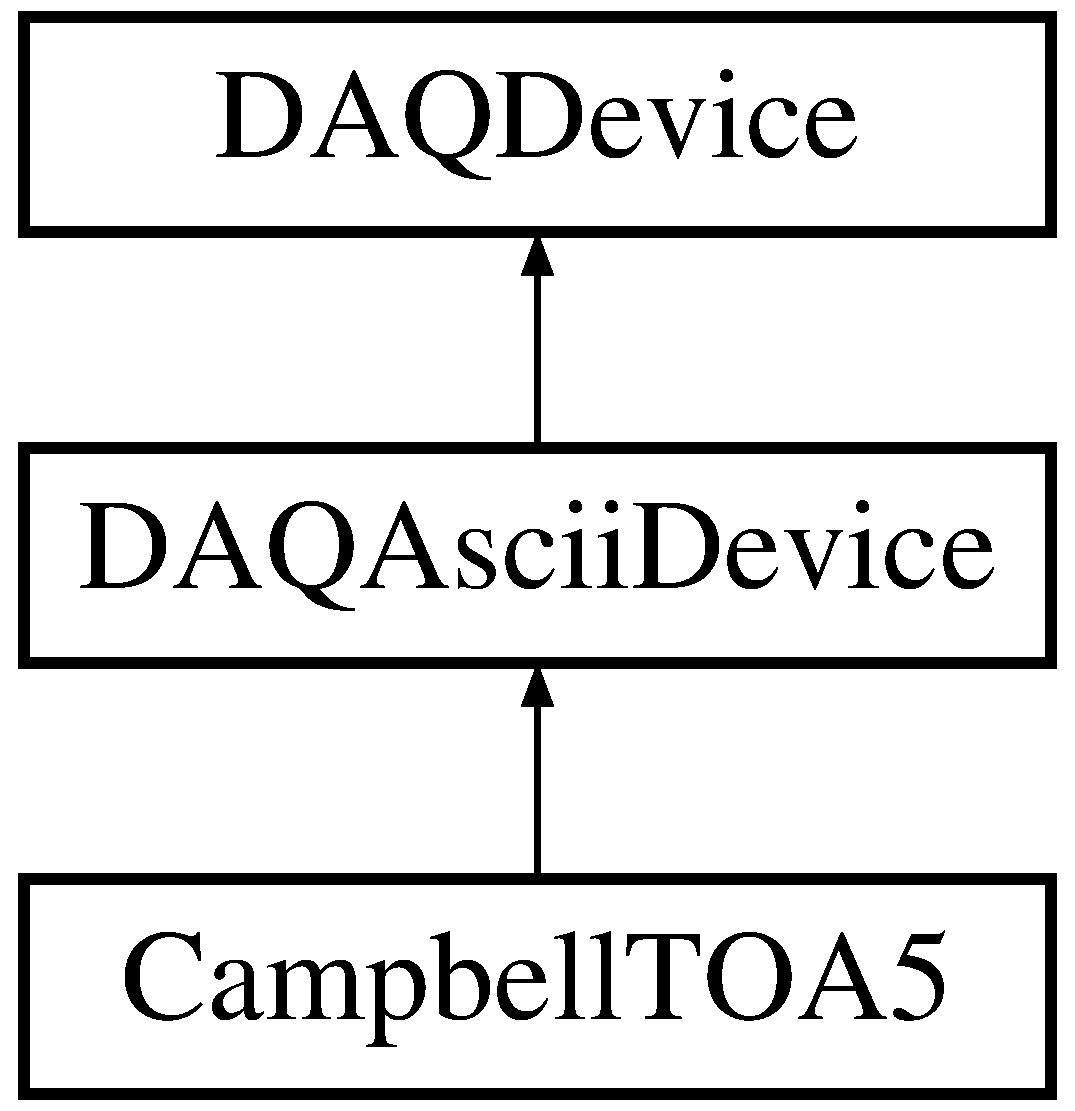
\includegraphics[height=3.000000cm]{classCampbellTOA5}
\end{center}
\end{figure}
\subsection*{Public Member Functions}
\begin{DoxyCompactItemize}
\item 
\hyperlink{classCampbellTOA5_ad53955c209a3f02a299989e03c47896e}{Campbell\-T\-O\-A5} ()
\item 
\hyperlink{classCampbellTOA5_a98f2239113ed206b37da17e24740da22}{$\sim$\-Campbell\-T\-O\-A5} ()
\item 
unsigned int \hyperlink{classCampbellTOA5_a97d66fcd7773a093d43f468e2998ae39}{get\-Sensor\-Group} ()
\item 
int \hyperlink{classCampbellTOA5_a3781a7ec4c685f52595aba01d46bad45}{read\-Header} (const char $\ast$header)
\end{DoxyCompactItemize}
\subsection*{Additional Inherited Members}


\subsection{Detailed Description}
Implementation of a reader for the Campbell Data\-Logger format A05. The format has compare to previous Campbell A\-S\-C\-I\-I formats more header information. 

\subsection{Constructor \& Destructor Documentation}
\hypertarget{classCampbellTOA5_ad53955c209a3f02a299989e03c47896e}{\index{Campbell\-T\-O\-A5@{Campbell\-T\-O\-A5}!Campbell\-T\-O\-A5@{Campbell\-T\-O\-A5}}
\index{Campbell\-T\-O\-A5@{Campbell\-T\-O\-A5}!CampbellTOA5@{Campbell\-T\-O\-A5}}
\subsubsection[{Campbell\-T\-O\-A5}]{\setlength{\rightskip}{0pt plus 5cm}Campbell\-T\-O\-A5\-::\-Campbell\-T\-O\-A5 (
\begin{DoxyParamCaption}
{}
\end{DoxyParamCaption}
)}}\label{classCampbellTOA5_ad53955c209a3f02a299989e03c47896e}
\hypertarget{classCampbellTOA5_a98f2239113ed206b37da17e24740da22}{\index{Campbell\-T\-O\-A5@{Campbell\-T\-O\-A5}!$\sim$\-Campbell\-T\-O\-A5@{$\sim$\-Campbell\-T\-O\-A5}}
\index{$\sim$\-Campbell\-T\-O\-A5@{$\sim$\-Campbell\-T\-O\-A5}!CampbellTOA5@{Campbell\-T\-O\-A5}}
\subsubsection[{$\sim$\-Campbell\-T\-O\-A5}]{\setlength{\rightskip}{0pt plus 5cm}Campbell\-T\-O\-A5\-::$\sim$\-Campbell\-T\-O\-A5 (
\begin{DoxyParamCaption}
{}
\end{DoxyParamCaption}
)}}\label{classCampbellTOA5_a98f2239113ed206b37da17e24740da22}


\subsection{Member Function Documentation}
\hypertarget{classCampbellTOA5_a97d66fcd7773a093d43f468e2998ae39}{\index{Campbell\-T\-O\-A5@{Campbell\-T\-O\-A5}!get\-Sensor\-Group@{get\-Sensor\-Group}}
\index{get\-Sensor\-Group@{get\-Sensor\-Group}!CampbellTOA5@{Campbell\-T\-O\-A5}}
\subsubsection[{get\-Sensor\-Group}]{\setlength{\rightskip}{0pt plus 5cm}unsigned int Campbell\-T\-O\-A5\-::get\-Sensor\-Group (
\begin{DoxyParamCaption}
{}
\end{DoxyParamCaption}
)\hspace{0.3cm}{\ttfamily [virtual]}}}\label{classCampbellTOA5_a97d66fcd7773a093d43f468e2998ae39}
Return the number of the sensor group 

Reimplemented from \hyperlink{classDAQDevice_a61d08492a11c30944dfaf3b86115abe8}{D\-A\-Q\-Device}.

\hypertarget{classCampbellTOA5_a3781a7ec4c685f52595aba01d46bad45}{\index{Campbell\-T\-O\-A5@{Campbell\-T\-O\-A5}!read\-Header@{read\-Header}}
\index{read\-Header@{read\-Header}!CampbellTOA5@{Campbell\-T\-O\-A5}}
\subsubsection[{read\-Header}]{\setlength{\rightskip}{0pt plus 5cm}int Campbell\-T\-O\-A5\-::read\-Header (
\begin{DoxyParamCaption}
\item[{const char $\ast$}]{header}
\end{DoxyParamCaption}
)\hspace{0.3cm}{\ttfamily [virtual]}}}\label{classCampbellTOA5_a3781a7ec4c685f52595aba01d46bad45}
Read Campbell specific header information 

Reimplemented from \hyperlink{classDAQAsciiDevice_a5fce725c52b70ef2f56a34b32a03e15d}{D\-A\-Q\-Ascii\-Device}.



The documentation for this class was generated from the following files\-:\begin{DoxyCompactItemize}
\item 
/home/ntj/\-Development/phd/kitcube-\/tools/src/kitcube-\/devices/\hyperlink{campbelltoa5_8h}{campbelltoa5.\-h}\item 
/home/ntj/\-Development/phd/kitcube-\/tools/src/kitcube-\/devices/\hyperlink{campbelltoa5_8cpp}{campbelltoa5.\-cpp}\end{DoxyCompactItemize}

\hypertarget{classCampbellTOB1}{\section{Campbell\-T\-O\-B1 Class Reference}
\label{classCampbellTOB1}\index{Campbell\-T\-O\-B1@{Campbell\-T\-O\-B1}}
}


{\ttfamily \#include $<$campbelltob1.\-h$>$}

Inheritance diagram for Campbell\-T\-O\-B1\-:\begin{figure}[H]
\begin{center}
\leavevmode
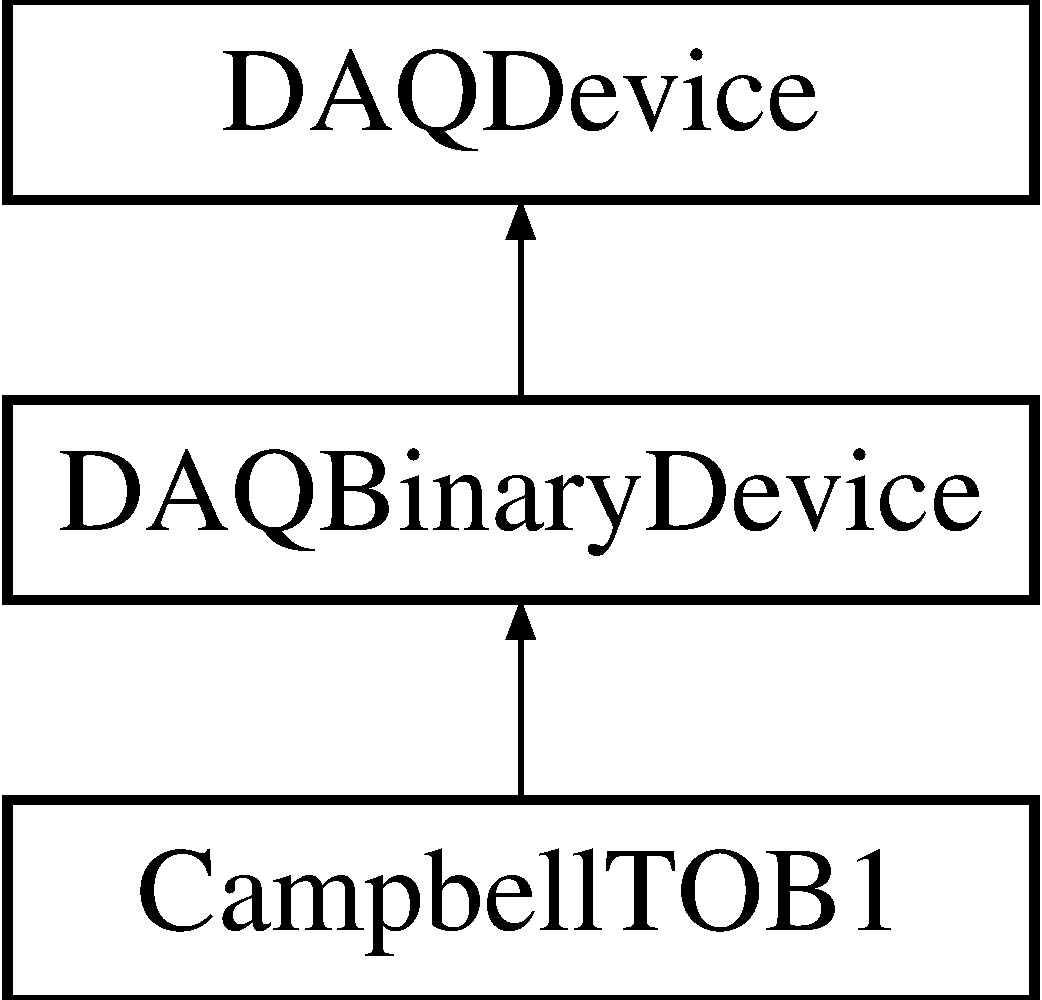
\includegraphics[height=3.000000cm]{classCampbellTOB1}
\end{center}
\end{figure}
\subsection*{Public Member Functions}
\begin{DoxyCompactItemize}
\item 
\hyperlink{classCampbellTOB1_a97fb5dfccd67207325b7db97c20fca72}{Campbell\-T\-O\-B1} ()
\item 
\hyperlink{classCampbellTOB1_a4ce5f8a2bd90b20b7ad2cf6ecb26ec7b}{$\sim$\-Campbell\-T\-O\-B1} ()
\item 
int \hyperlink{classCampbellTOB1_aad343912437691a763b7130deec5372c}{read\-Header} (const char $\ast$header)
\end{DoxyCompactItemize}
\subsection*{Additional Inherited Members}


\subsection{Detailed Description}
Implementation of a reader for the Campbell Data\-Logger format T\-O\-B3 / T\-O\-Bx?. The format has compare to previous Campbell A\-S\-C\-I\-I formats more header information. 

\subsection{Constructor \& Destructor Documentation}
\hypertarget{classCampbellTOB1_a97fb5dfccd67207325b7db97c20fca72}{\index{Campbell\-T\-O\-B1@{Campbell\-T\-O\-B1}!Campbell\-T\-O\-B1@{Campbell\-T\-O\-B1}}
\index{Campbell\-T\-O\-B1@{Campbell\-T\-O\-B1}!CampbellTOB1@{Campbell\-T\-O\-B1}}
\subsubsection[{Campbell\-T\-O\-B1}]{\setlength{\rightskip}{0pt plus 5cm}Campbell\-T\-O\-B1\-::\-Campbell\-T\-O\-B1 (
\begin{DoxyParamCaption}
{}
\end{DoxyParamCaption}
)}}\label{classCampbellTOB1_a97fb5dfccd67207325b7db97c20fca72}
\hypertarget{classCampbellTOB1_a4ce5f8a2bd90b20b7ad2cf6ecb26ec7b}{\index{Campbell\-T\-O\-B1@{Campbell\-T\-O\-B1}!$\sim$\-Campbell\-T\-O\-B1@{$\sim$\-Campbell\-T\-O\-B1}}
\index{$\sim$\-Campbell\-T\-O\-B1@{$\sim$\-Campbell\-T\-O\-B1}!CampbellTOB1@{Campbell\-T\-O\-B1}}
\subsubsection[{$\sim$\-Campbell\-T\-O\-B1}]{\setlength{\rightskip}{0pt plus 5cm}Campbell\-T\-O\-B1\-::$\sim$\-Campbell\-T\-O\-B1 (
\begin{DoxyParamCaption}
{}
\end{DoxyParamCaption}
)}}\label{classCampbellTOB1_a4ce5f8a2bd90b20b7ad2cf6ecb26ec7b}


\subsection{Member Function Documentation}
\hypertarget{classCampbellTOB1_aad343912437691a763b7130deec5372c}{\index{Campbell\-T\-O\-B1@{Campbell\-T\-O\-B1}!read\-Header@{read\-Header}}
\index{read\-Header@{read\-Header}!CampbellTOB1@{Campbell\-T\-O\-B1}}
\subsubsection[{read\-Header}]{\setlength{\rightskip}{0pt plus 5cm}int Campbell\-T\-O\-B1\-::read\-Header (
\begin{DoxyParamCaption}
\item[{const char $\ast$}]{header}
\end{DoxyParamCaption}
)\hspace{0.3cm}{\ttfamily [virtual]}}}\label{classCampbellTOB1_aad343912437691a763b7130deec5372c}
Read Campbell specific header information 

Reimplemented from \hyperlink{classDAQDevice_af5fa373af9a089c18c7fd1d662db144f}{D\-A\-Q\-Device}.



The documentation for this class was generated from the following files\-:\begin{DoxyCompactItemize}
\item 
/home/ntj/\-Development/phd/kitcube-\/tools/src/kitcube-\/devices/\hyperlink{campbelltob1_8h}{campbelltob1.\-h}\item 
/home/ntj/\-Development/phd/kitcube-\/tools/src/kitcube-\/devices/\hyperlink{campbelltob1_8cpp}{campbelltob1.\-cpp}\end{DoxyCompactItemize}

\hypertarget{classCeilometer}{\section{Ceilometer Class Reference}
\label{classCeilometer}\index{Ceilometer@{Ceilometer}}
}


{\ttfamily \#include $<$ceilometer.\-h$>$}

Inheritance diagram for Ceilometer\-:\begin{figure}[H]
\begin{center}
\leavevmode
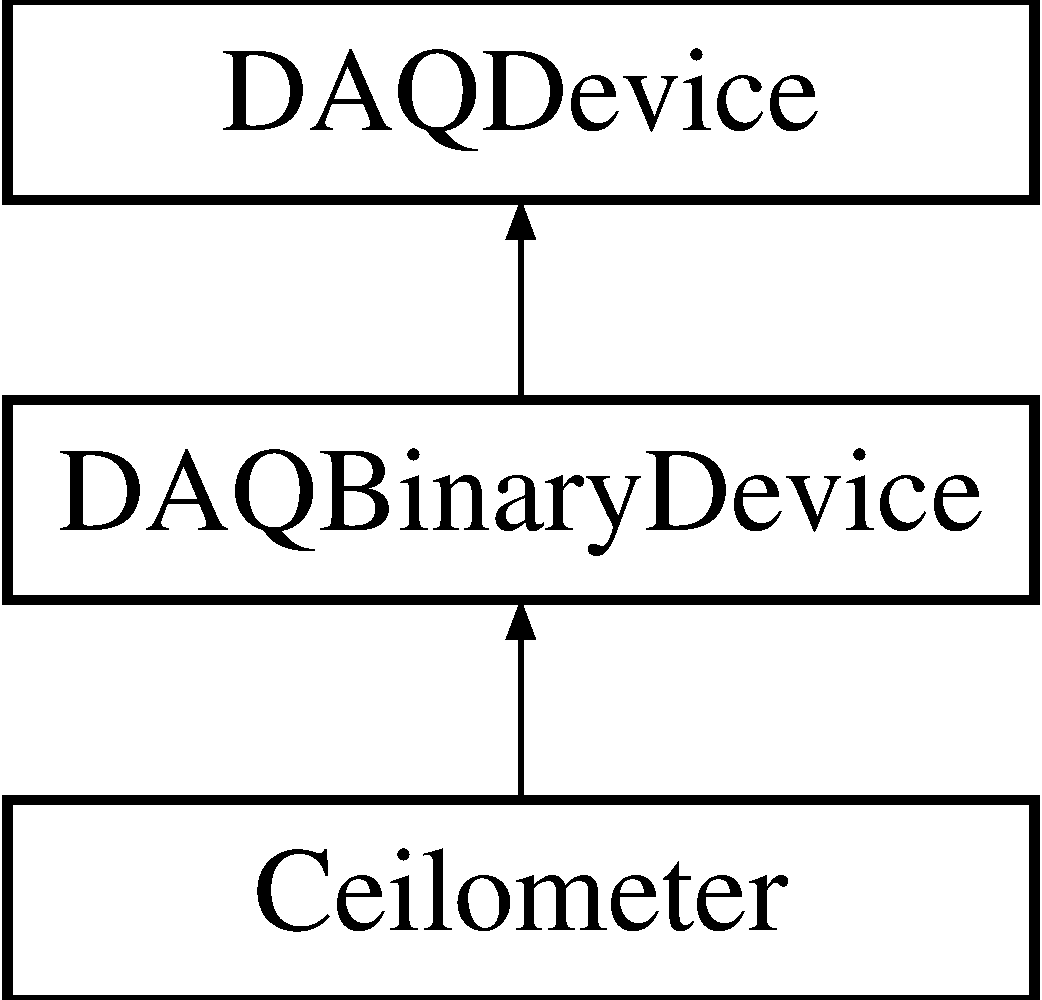
\includegraphics[height=3.000000cm]{classCeilometer}
\end{center}
\end{figure}
\subsection*{Public Member Functions}
\begin{DoxyCompactItemize}
\item 
\hyperlink{classCeilometer_a2bf3db4a3f55c934412f83553f531f2b}{Ceilometer} ()
\item 
\hyperlink{classCeilometer_a449bdf7592f4630df99ab15bc885445b}{$\sim$\-Ceilometer} ()
\item 
void \hyperlink{classCeilometer_a9e1c96a6f8e813ac7490dfda84f9455b}{set\-Config\-Defaults} ()
\item 
const char $\ast$ \hyperlink{classCeilometer_ac9984aad78fe229d7314d45c0e722ef2}{get\-Data\-Dir} ()
\item 
void \hyperlink{classCeilometer_a50863be019de8c71409e73ffd1e83921}{replace\-Item} (const char $\ast$$\ast$header, const char $\ast$item\-Tag, const char $\ast$new\-Value)
\item 
const char $\ast$ \hyperlink{classCeilometer_a739c17f98b60c5cbcd3d65d6973dc22b}{get\-String\-Item} (const char $\ast$$\ast$header, const char $\ast$item\-Tag)
\item 
int \hyperlink{classCeilometer_ab35f4b64b941194185aee79ed3002456}{get\-Numeric\-Item} (const char $\ast$$\ast$header, const char $\ast$item\-Tag)
\item 
unsigned int \hyperlink{classCeilometer_a4acd8818fb18be80d3cc442d71934657}{get\-Sensor\-Group} ()
\item 
int \hyperlink{classCeilometer_ac915ac4f192b4e59d7cd40ed022a045d}{read\-Header} (const char $\ast$header)
\item 
void \hyperlink{classCeilometer_ab114fc34cce9cdb8ed87cad3aab908d0}{write\-Header} ()
\item 
void \hyperlink{classCeilometer_a9ef73907ba808f6f967b32dc3a161a66}{read\-Data} (std\-::string full\-\_\-filename)
\item 
void \hyperlink{classCeilometer_aeb9c0bddc60b920f7d686a7663b37eae}{read\-Netcdf} (std\-::string full\-\_\-filename)
\item 
int \hyperlink{classCeilometer_aaff1b4b73350c443e64df5decd975f07}{parse\-Data} (char $\ast$line, struct timeval $\ast$l\-\_\-t\-Data, double $\ast$\hyperlink{classDAQDevice_ad148188c57598fdf4fd4c1c333aeb0d8}{sensor\-Value})
\item 
void \hyperlink{classCeilometer_adcb425b5d5ffeb84a3603bab2a5ae6df}{update\-Data\-Set} (unsigned char $\ast$buf)
\end{DoxyCompactItemize}
\subsection*{Private Attributes}
\begin{DoxyCompactItemize}
\item 
unsigned char $\ast$ \hyperlink{classCeilometer_ae6363cb7019753e8d2b1b005d030818e}{header\-Raw}
\item 
std\-::string \hyperlink{classCeilometer_adacde94d57006bd9d81a20919bcb4f20}{experiment\-Name}
\item 
unsigned long \hyperlink{classCeilometer_ab98f876944333787e16570753c409560}{t\-Sample}
\item 
struct timeval \hyperlink{classCeilometer_a173231c1db65165d1a0cb91d3913339e}{t\-Ref}
\end{DoxyCompactItemize}
\subsection*{Additional Inherited Members}


\subsection{Detailed Description}
Implementation for the ceilometer D\-A\-Q device.

\begin{DoxyRefDesc}{Todo}
\item[\hyperlink{todo__todo000015}{Todo}]Move return string to the argument list\end{DoxyRefDesc}


\subsection{Constructor \& Destructor Documentation}
\hypertarget{classCeilometer_a2bf3db4a3f55c934412f83553f531f2b}{\index{Ceilometer@{Ceilometer}!Ceilometer@{Ceilometer}}
\index{Ceilometer@{Ceilometer}!Ceilometer@{Ceilometer}}
\subsubsection[{Ceilometer}]{\setlength{\rightskip}{0pt plus 5cm}Ceilometer\-::\-Ceilometer (
\begin{DoxyParamCaption}
{}
\end{DoxyParamCaption}
)}}\label{classCeilometer_a2bf3db4a3f55c934412f83553f531f2b}
\hypertarget{classCeilometer_a449bdf7592f4630df99ab15bc885445b}{\index{Ceilometer@{Ceilometer}!$\sim$\-Ceilometer@{$\sim$\-Ceilometer}}
\index{$\sim$\-Ceilometer@{$\sim$\-Ceilometer}!Ceilometer@{Ceilometer}}
\subsubsection[{$\sim$\-Ceilometer}]{\setlength{\rightskip}{0pt plus 5cm}Ceilometer\-::$\sim$\-Ceilometer (
\begin{DoxyParamCaption}
{}
\end{DoxyParamCaption}
)}}\label{classCeilometer_a449bdf7592f4630df99ab15bc885445b}


\subsection{Member Function Documentation}
\hypertarget{classCeilometer_ac9984aad78fe229d7314d45c0e722ef2}{\index{Ceilometer@{Ceilometer}!get\-Data\-Dir@{get\-Data\-Dir}}
\index{get\-Data\-Dir@{get\-Data\-Dir}!Ceilometer@{Ceilometer}}
\subsubsection[{get\-Data\-Dir}]{\setlength{\rightskip}{0pt plus 5cm}const char $\ast$ Ceilometer\-::get\-Data\-Dir (
\begin{DoxyParamCaption}
{}
\end{DoxyParamCaption}
)\hspace{0.3cm}{\ttfamily [virtual]}}}\label{classCeilometer_ac9984aad78fe229d7314d45c0e722ef2}
Read parameter from inifile Returns the path relative to the base path to the data dir 

Reimplemented from \hyperlink{classDAQDevice_a7d7d41f0c1496221e589d84b38d1c865}{D\-A\-Q\-Device}.

\hypertarget{classCeilometer_ab35f4b64b941194185aee79ed3002456}{\index{Ceilometer@{Ceilometer}!get\-Numeric\-Item@{get\-Numeric\-Item}}
\index{get\-Numeric\-Item@{get\-Numeric\-Item}!Ceilometer@{Ceilometer}}
\subsubsection[{get\-Numeric\-Item}]{\setlength{\rightskip}{0pt plus 5cm}int Ceilometer\-::get\-Numeric\-Item (
\begin{DoxyParamCaption}
\item[{const char $\ast$$\ast$}]{header, }
\item[{const char $\ast$}]{item\-Tag}
\end{DoxyParamCaption}
)}}\label{classCeilometer_ab35f4b64b941194185aee79ed3002456}
\hypertarget{classCeilometer_a4acd8818fb18be80d3cc442d71934657}{\index{Ceilometer@{Ceilometer}!get\-Sensor\-Group@{get\-Sensor\-Group}}
\index{get\-Sensor\-Group@{get\-Sensor\-Group}!Ceilometer@{Ceilometer}}
\subsubsection[{get\-Sensor\-Group}]{\setlength{\rightskip}{0pt plus 5cm}unsigned int Ceilometer\-::get\-Sensor\-Group (
\begin{DoxyParamCaption}
{}
\end{DoxyParamCaption}
)\hspace{0.3cm}{\ttfamily [virtual]}}}\label{classCeilometer_a4acd8818fb18be80d3cc442d71934657}
Define a sensor group number for all the availble sensor group files 

Reimplemented from \hyperlink{classDAQDevice_a61d08492a11c30944dfaf3b86115abe8}{D\-A\-Q\-Device}.

\hypertarget{classCeilometer_a739c17f98b60c5cbcd3d65d6973dc22b}{\index{Ceilometer@{Ceilometer}!get\-String\-Item@{get\-String\-Item}}
\index{get\-String\-Item@{get\-String\-Item}!Ceilometer@{Ceilometer}}
\subsubsection[{get\-String\-Item}]{\setlength{\rightskip}{0pt plus 5cm}const char $\ast$ Ceilometer\-::get\-String\-Item (
\begin{DoxyParamCaption}
\item[{const char $\ast$$\ast$}]{header, }
\item[{const char $\ast$}]{item\-Tag}
\end{DoxyParamCaption}
)}}\label{classCeilometer_a739c17f98b60c5cbcd3d65d6973dc22b}
\hypertarget{classCeilometer_aaff1b4b73350c443e64df5decd975f07}{\index{Ceilometer@{Ceilometer}!parse\-Data@{parse\-Data}}
\index{parse\-Data@{parse\-Data}!Ceilometer@{Ceilometer}}
\subsubsection[{parse\-Data}]{\setlength{\rightskip}{0pt plus 5cm}int Ceilometer\-::parse\-Data (
\begin{DoxyParamCaption}
\item[{char $\ast$}]{line, }
\item[{struct timeval $\ast$}]{l\-\_\-t\-Data, }
\item[{double $\ast$}]{sensor\-Value}
\end{DoxyParamCaption}
)\hspace{0.3cm}{\ttfamily [virtual]}}}\label{classCeilometer_aaff1b4b73350c443e64df5decd975f07}
Read the data from the current line of the data file. \begin{DoxyReturn}{Returns}
-\/1 no data found, skip storage 0 sucess, store data, 1 read another line 
\end{DoxyReturn}


Reimplemented from \hyperlink{classDAQDevice_a37f6fcab4893285e7f7d74670294a645}{D\-A\-Q\-Device}.

\hypertarget{classCeilometer_a9ef73907ba808f6f967b32dc3a161a66}{\index{Ceilometer@{Ceilometer}!read\-Data@{read\-Data}}
\index{read\-Data@{read\-Data}!Ceilometer@{Ceilometer}}
\subsubsection[{read\-Data}]{\setlength{\rightskip}{0pt plus 5cm}void Ceilometer\-::read\-Data (
\begin{DoxyParamCaption}
\item[{std\-::string}]{full\-\_\-filename}
\end{DoxyParamCaption}
)\hspace{0.3cm}{\ttfamily [virtual]}}}\label{classCeilometer_a9ef73907ba808f6f967b32dc3a161a66}


Reimplemented from \hyperlink{classDAQBinaryDevice_a725281822b7945b8c1154d079c0011ff}{D\-A\-Q\-Binary\-Device}.

\hypertarget{classCeilometer_ac915ac4f192b4e59d7cd40ed022a045d}{\index{Ceilometer@{Ceilometer}!read\-Header@{read\-Header}}
\index{read\-Header@{read\-Header}!Ceilometer@{Ceilometer}}
\subsubsection[{read\-Header}]{\setlength{\rightskip}{0pt plus 5cm}int Ceilometer\-::read\-Header (
\begin{DoxyParamCaption}
\item[{const char $\ast$}]{header}
\end{DoxyParamCaption}
)\hspace{0.3cm}{\ttfamily [virtual]}}}\label{classCeilometer_ac915ac4f192b4e59d7cd40ed022a045d}
Get time until next sample and it's id 

Reimplemented from \hyperlink{classDAQDevice_af5fa373af9a089c18c7fd1d662db144f}{D\-A\-Q\-Device}.

\hypertarget{classCeilometer_aeb9c0bddc60b920f7d686a7663b37eae}{\index{Ceilometer@{Ceilometer}!read\-Netcdf@{read\-Netcdf}}
\index{read\-Netcdf@{read\-Netcdf}!Ceilometer@{Ceilometer}}
\subsubsection[{read\-Netcdf}]{\setlength{\rightskip}{0pt plus 5cm}void Ceilometer\-::read\-Netcdf (
\begin{DoxyParamCaption}
\item[{std\-::string}]{full\-\_\-filename}
\end{DoxyParamCaption}
)}}\label{classCeilometer_aeb9c0bddc60b920f7d686a7663b37eae}
\hypertarget{classCeilometer_a50863be019de8c71409e73ffd1e83921}{\index{Ceilometer@{Ceilometer}!replace\-Item@{replace\-Item}}
\index{replace\-Item@{replace\-Item}!Ceilometer@{Ceilometer}}
\subsubsection[{replace\-Item}]{\setlength{\rightskip}{0pt plus 5cm}void Ceilometer\-::replace\-Item (
\begin{DoxyParamCaption}
\item[{const char $\ast$$\ast$}]{header, }
\item[{const char $\ast$}]{item\-Tag, }
\item[{const char $\ast$}]{new\-Value}
\end{DoxyParamCaption}
)}}\label{classCeilometer_a50863be019de8c71409e73ffd1e83921}
\hypertarget{classCeilometer_a9e1c96a6f8e813ac7490dfda84f9455b}{\index{Ceilometer@{Ceilometer}!set\-Config\-Defaults@{set\-Config\-Defaults}}
\index{set\-Config\-Defaults@{set\-Config\-Defaults}!Ceilometer@{Ceilometer}}
\subsubsection[{set\-Config\-Defaults}]{\setlength{\rightskip}{0pt plus 5cm}void Ceilometer\-::set\-Config\-Defaults (
\begin{DoxyParamCaption}
{}
\end{DoxyParamCaption}
)\hspace{0.3cm}{\ttfamily [virtual]}}}\label{classCeilometer_a9e1c96a6f8e813ac7490dfda84f9455b}
Set default configuration 

Reimplemented from \hyperlink{classDAQDevice_a7685cec80865752cc0ef3ab49c6c2277}{D\-A\-Q\-Device}.

\hypertarget{classCeilometer_adcb425b5d5ffeb84a3603bab2a5ae6df}{\index{Ceilometer@{Ceilometer}!update\-Data\-Set@{update\-Data\-Set}}
\index{update\-Data\-Set@{update\-Data\-Set}!Ceilometer@{Ceilometer}}
\subsubsection[{update\-Data\-Set}]{\setlength{\rightskip}{0pt plus 5cm}void Ceilometer\-::update\-Data\-Set (
\begin{DoxyParamCaption}
\item[{unsigned char $\ast$}]{buf}
\end{DoxyParamCaption}
)\hspace{0.3cm}{\ttfamily [virtual]}}}\label{classCeilometer_adcb425b5d5ffeb84a3603bab2a5ae6df}
Replace time stamp in the data set by the current time 

Reimplemented from \hyperlink{classDAQDevice_a06d18d7b372d35c55f8a1a399f582a94}{D\-A\-Q\-Device}.

\hypertarget{classCeilometer_ab114fc34cce9cdb8ed87cad3aab908d0}{\index{Ceilometer@{Ceilometer}!write\-Header@{write\-Header}}
\index{write\-Header@{write\-Header}!Ceilometer@{Ceilometer}}
\subsubsection[{write\-Header}]{\setlength{\rightskip}{0pt plus 5cm}void Ceilometer\-::write\-Header (
\begin{DoxyParamCaption}
{}
\end{DoxyParamCaption}
)\hspace{0.3cm}{\ttfamily [virtual]}}}\label{classCeilometer_ab114fc34cce9cdb8ed87cad3aab908d0}


Reimplemented from \hyperlink{classDAQDevice_aad39c13f039abd6e6a9b0aa21a7c8a4d}{D\-A\-Q\-Device}.



\subsection{Member Data Documentation}
\hypertarget{classCeilometer_adacde94d57006bd9d81a20919bcb4f20}{\index{Ceilometer@{Ceilometer}!experiment\-Name@{experiment\-Name}}
\index{experiment\-Name@{experiment\-Name}!Ceilometer@{Ceilometer}}
\subsubsection[{experiment\-Name}]{\setlength{\rightskip}{0pt plus 5cm}std\-::string Ceilometer\-::experiment\-Name\hspace{0.3cm}{\ttfamily [private]}}}\label{classCeilometer_adacde94d57006bd9d81a20919bcb4f20}
\hypertarget{classCeilometer_ae6363cb7019753e8d2b1b005d030818e}{\index{Ceilometer@{Ceilometer}!header\-Raw@{header\-Raw}}
\index{header\-Raw@{header\-Raw}!Ceilometer@{Ceilometer}}
\subsubsection[{header\-Raw}]{\setlength{\rightskip}{0pt plus 5cm}unsigned char$\ast$ Ceilometer\-::header\-Raw\hspace{0.3cm}{\ttfamily [private]}}}\label{classCeilometer_ae6363cb7019753e8d2b1b005d030818e}
\hypertarget{classCeilometer_a173231c1db65165d1a0cb91d3913339e}{\index{Ceilometer@{Ceilometer}!t\-Ref@{t\-Ref}}
\index{t\-Ref@{t\-Ref}!Ceilometer@{Ceilometer}}
\subsubsection[{t\-Ref}]{\setlength{\rightskip}{0pt plus 5cm}struct timeval Ceilometer\-::t\-Ref\hspace{0.3cm}{\ttfamily [private]}}}\label{classCeilometer_a173231c1db65165d1a0cb91d3913339e}
\hypertarget{classCeilometer_ab98f876944333787e16570753c409560}{\index{Ceilometer@{Ceilometer}!t\-Sample@{t\-Sample}}
\index{t\-Sample@{t\-Sample}!Ceilometer@{Ceilometer}}
\subsubsection[{t\-Sample}]{\setlength{\rightskip}{0pt plus 5cm}unsigned long Ceilometer\-::t\-Sample\hspace{0.3cm}{\ttfamily [private]}}}\label{classCeilometer_ab98f876944333787e16570753c409560}


The documentation for this class was generated from the following files\-:\begin{DoxyCompactItemize}
\item 
/home/ntj/\-Development/phd/kitcube-\/tools/src/kitcube-\/devices/\hyperlink{ceilometer_8h}{ceilometer.\-h}\item 
/home/ntj/\-Development/phd/kitcube-\/tools/src/kitcube-\/devices/\hyperlink{ceilometer_8cpp}{ceilometer.\-cpp}\end{DoxyCompactItemize}

\hypertarget{structConfigurationRecord}{\section{Configuration\-Record Struct Reference}
\label{structConfigurationRecord}\index{Configuration\-Record@{Configuration\-Record}}
}


{\ttfamily \#include $<$windtracer.\-h$>$}

\subsection*{Public Attributes}
\begin{DoxyCompactItemize}
\item 
struct \hyperlink{structBlockDescriptor}{Block\-Descriptor} \hyperlink{structConfigurationRecord_a1e8e13368061b97fa7d2763bb5152e2a}{block\-\_\-desc}
\item 
char $\ast$ \hyperlink{structConfigurationRecord_a961d871fc719aa11527c52830df1bcb9}{ch\-Configuration}
\end{DoxyCompactItemize}


\subsection{Member Data Documentation}
\hypertarget{structConfigurationRecord_a1e8e13368061b97fa7d2763bb5152e2a}{\index{Configuration\-Record@{Configuration\-Record}!block\-\_\-desc@{block\-\_\-desc}}
\index{block\-\_\-desc@{block\-\_\-desc}!ConfigurationRecord@{Configuration\-Record}}
\subsubsection[{block\-\_\-desc}]{\setlength{\rightskip}{0pt plus 5cm}struct {\bf Block\-Descriptor} Configuration\-Record\-::block\-\_\-desc}}\label{structConfigurationRecord_a1e8e13368061b97fa7d2763bb5152e2a}
\hypertarget{structConfigurationRecord_a961d871fc719aa11527c52830df1bcb9}{\index{Configuration\-Record@{Configuration\-Record}!ch\-Configuration@{ch\-Configuration}}
\index{ch\-Configuration@{ch\-Configuration}!ConfigurationRecord@{Configuration\-Record}}
\subsubsection[{ch\-Configuration}]{\setlength{\rightskip}{0pt plus 5cm}char$\ast$ Configuration\-Record\-::ch\-Configuration}}\label{structConfigurationRecord_a961d871fc719aa11527c52830df1bcb9}


The documentation for this struct was generated from the following file\-:\begin{DoxyCompactItemize}
\item 
/home/ntj/\-Development/phd/kitcube-\/tools/src/kitcube-\/devices/\hyperlink{windtracer_8h}{windtracer.\-h}\end{DoxyCompactItemize}

\hypertarget{classDAQAsciiDevice}{\section{D\-A\-Q\-Ascii\-Device Class Reference}
\label{classDAQAsciiDevice}\index{D\-A\-Q\-Ascii\-Device@{D\-A\-Q\-Ascii\-Device}}
}


{\ttfamily \#include $<$daqasciidevice.\-h$>$}

Inheritance diagram for D\-A\-Q\-Ascii\-Device\-:\begin{figure}[H]
\begin{center}
\leavevmode
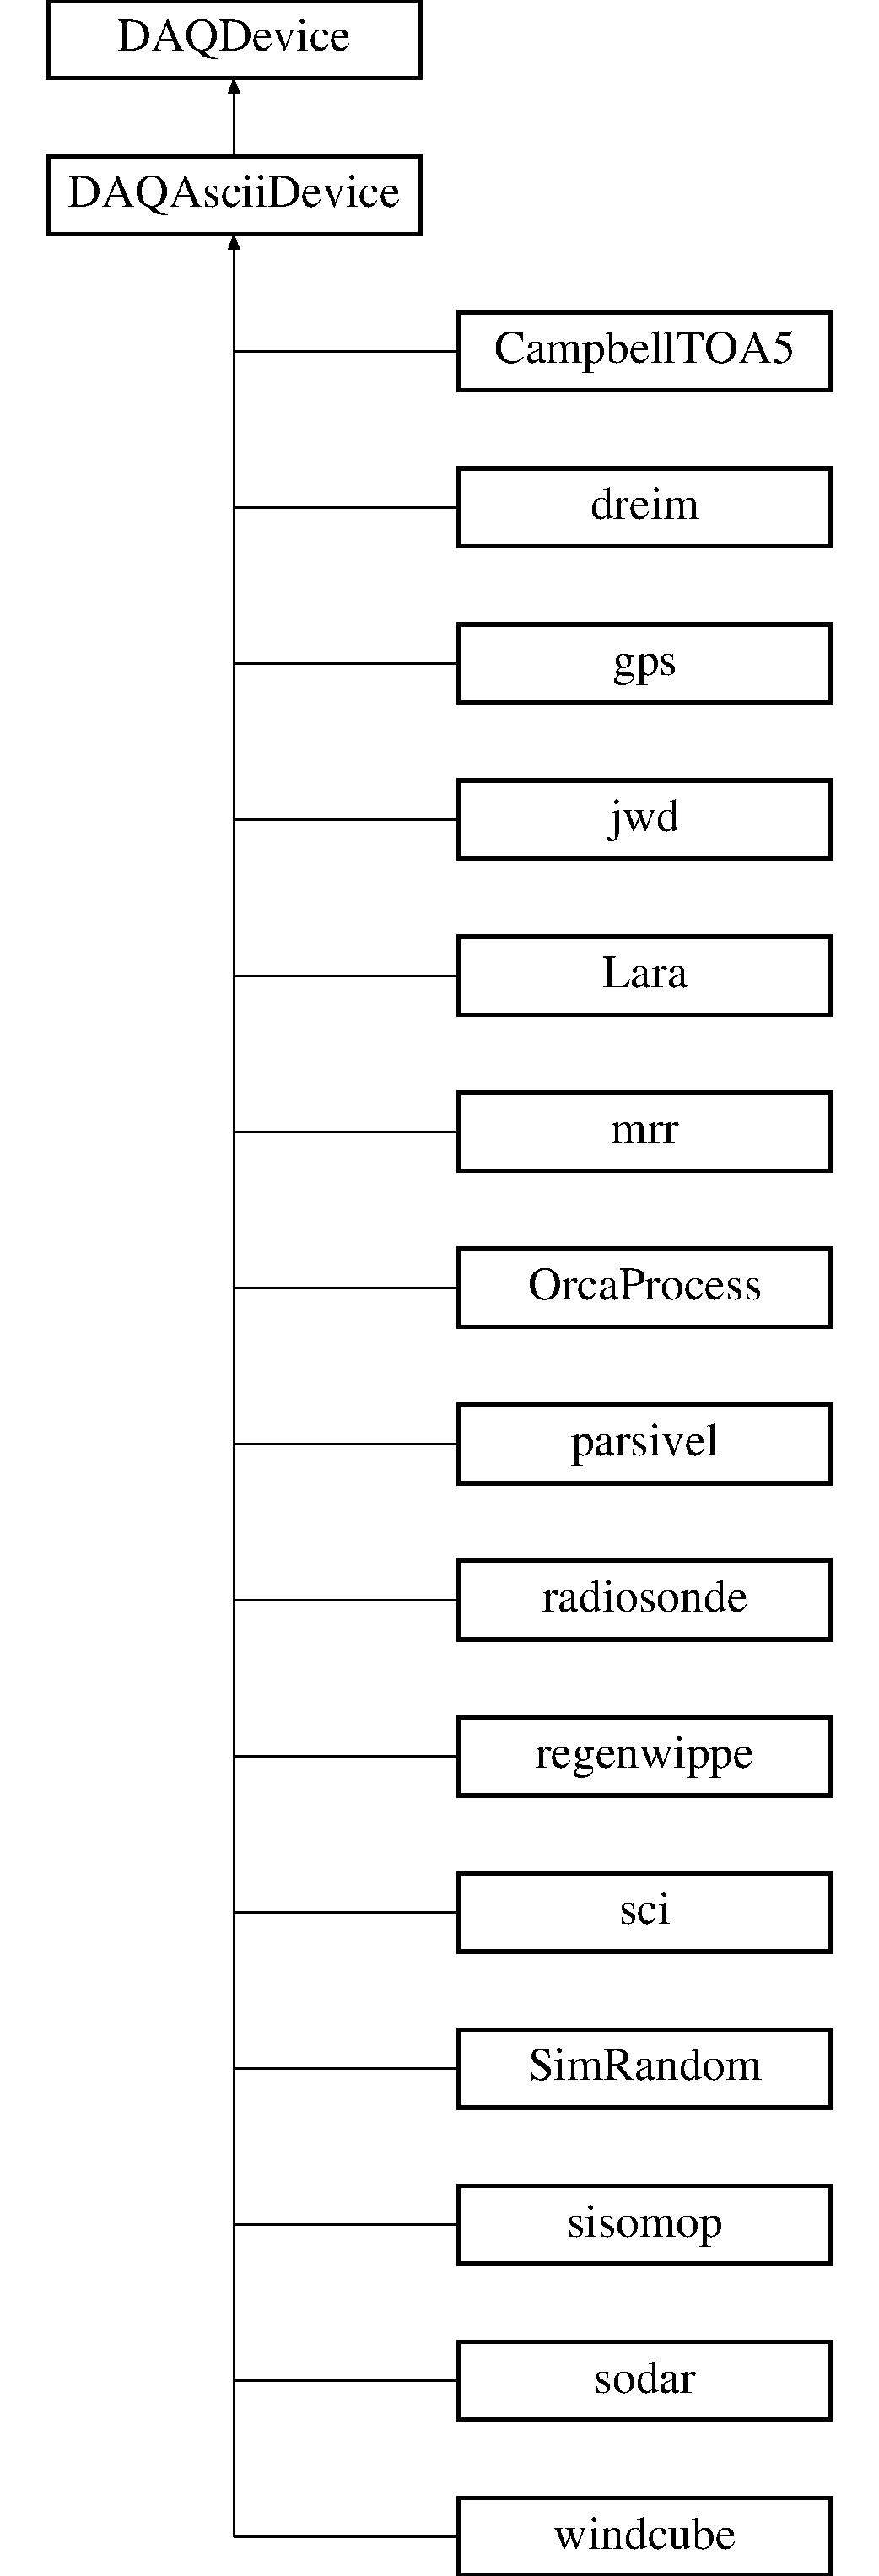
\includegraphics[height=12.000000cm]{classDAQAsciiDevice}
\end{center}
\end{figure}
\subsection*{Public Member Functions}
\begin{DoxyCompactItemize}
\item 
\hyperlink{classDAQAsciiDevice_adaef2eca0f5c36b4e8aeebc72e87707c}{D\-A\-Q\-Ascii\-Device} ()
\item 
\hyperlink{classDAQAsciiDevice_a1fb0f1abaeb456ec194f64718c68128d}{$\sim$\-D\-A\-Q\-Ascii\-Device} ()
\item 
virtual void \hyperlink{classDAQAsciiDevice_ae79f6ea28b8f477b5eda360a0a5e5854}{open\-File} ()
\item 
virtual void \hyperlink{classDAQAsciiDevice_aef686b204dd3569291c5cc4534f7aa24}{close\-File} ()
\item 
virtual int \hyperlink{classDAQAsciiDevice_a5fce725c52b70ef2f56a34b32a03e15d}{read\-Header} (const char $\ast$header)
\item 
virtual int \hyperlink{classDAQAsciiDevice_a9c20d9d69af4ba1641dbc82dd5be2aa5}{parse\-Data} (char $\ast$line, struct timeval $\ast$l\-\_\-t\-Data, double $\ast$\hyperlink{classDAQDevice_ad148188c57598fdf4fd4c1c333aeb0d8}{sensor\-Value})
\item 
virtual void \hyperlink{classDAQAsciiDevice_a0d9b17803680d966c7025ca6f174cef0}{read\-Data} (std\-::string full\-\_\-filename)
\end{DoxyCompactItemize}
\subsection*{Protected Attributes}
\begin{DoxyCompactItemize}
\item 
int \hyperlink{classDAQAsciiDevice_aa683d088c84eeea43836ad7dbe804800}{fd\-\_\-data}
\item 
unsigned long \hyperlink{classDAQAsciiDevice_ad7c5b15ad8e21ca0ecbf52afec874543}{n\-Samples}
\item 
unsigned long \hyperlink{classDAQAsciiDevice_a7885676e316cf2533707297f30f96644}{n\-Template}
\item 
int \hyperlink{classDAQAsciiDevice_a2dd49b3ae40e05dfd2e761f350d4320b}{n\-Map}
\item 
int $\ast$ \hyperlink{classDAQAsciiDevice_a50307e0ce456fb3fe201f4acd0716058}{dyn\-Map}
\end{DoxyCompactItemize}
\subsection*{Additional Inherited Members}


\subsection{Constructor \& Destructor Documentation}
\hypertarget{classDAQAsciiDevice_adaef2eca0f5c36b4e8aeebc72e87707c}{\index{D\-A\-Q\-Ascii\-Device@{D\-A\-Q\-Ascii\-Device}!D\-A\-Q\-Ascii\-Device@{D\-A\-Q\-Ascii\-Device}}
\index{D\-A\-Q\-Ascii\-Device@{D\-A\-Q\-Ascii\-Device}!DAQAsciiDevice@{D\-A\-Q\-Ascii\-Device}}
\subsubsection[{D\-A\-Q\-Ascii\-Device}]{\setlength{\rightskip}{0pt plus 5cm}D\-A\-Q\-Ascii\-Device\-::\-D\-A\-Q\-Ascii\-Device (
\begin{DoxyParamCaption}
{}
\end{DoxyParamCaption}
)}}\label{classDAQAsciiDevice_adaef2eca0f5c36b4e8aeebc72e87707c}
\hypertarget{classDAQAsciiDevice_a1fb0f1abaeb456ec194f64718c68128d}{\index{D\-A\-Q\-Ascii\-Device@{D\-A\-Q\-Ascii\-Device}!$\sim$\-D\-A\-Q\-Ascii\-Device@{$\sim$\-D\-A\-Q\-Ascii\-Device}}
\index{$\sim$\-D\-A\-Q\-Ascii\-Device@{$\sim$\-D\-A\-Q\-Ascii\-Device}!DAQAsciiDevice@{D\-A\-Q\-Ascii\-Device}}
\subsubsection[{$\sim$\-D\-A\-Q\-Ascii\-Device}]{\setlength{\rightskip}{0pt plus 5cm}D\-A\-Q\-Ascii\-Device\-::$\sim$\-D\-A\-Q\-Ascii\-Device (
\begin{DoxyParamCaption}
{}
\end{DoxyParamCaption}
)}}\label{classDAQAsciiDevice_a1fb0f1abaeb456ec194f64718c68128d}


\subsection{Member Function Documentation}
\hypertarget{classDAQAsciiDevice_aef686b204dd3569291c5cc4534f7aa24}{\index{D\-A\-Q\-Ascii\-Device@{D\-A\-Q\-Ascii\-Device}!close\-File@{close\-File}}
\index{close\-File@{close\-File}!DAQAsciiDevice@{D\-A\-Q\-Ascii\-Device}}
\subsubsection[{close\-File}]{\setlength{\rightskip}{0pt plus 5cm}void D\-A\-Q\-Ascii\-Device\-::close\-File (
\begin{DoxyParamCaption}
{}
\end{DoxyParamCaption}
)\hspace{0.3cm}{\ttfamily [virtual]}}}\label{classDAQAsciiDevice_aef686b204dd3569291c5cc4534f7aa24}
Close file for reading 

Reimplemented from \hyperlink{classDAQDevice_ae27c5729563be895c0d0a607ee023e30}{D\-A\-Q\-Device}.

\hypertarget{classDAQAsciiDevice_ae79f6ea28b8f477b5eda360a0a5e5854}{\index{D\-A\-Q\-Ascii\-Device@{D\-A\-Q\-Ascii\-Device}!open\-File@{open\-File}}
\index{open\-File@{open\-File}!DAQAsciiDevice@{D\-A\-Q\-Ascii\-Device}}
\subsubsection[{open\-File}]{\setlength{\rightskip}{0pt plus 5cm}void D\-A\-Q\-Ascii\-Device\-::open\-File (
\begin{DoxyParamCaption}
{}
\end{DoxyParamCaption}
)\hspace{0.3cm}{\ttfamily [virtual]}}}\label{classDAQAsciiDevice_ae79f6ea28b8f477b5eda360a0a5e5854}
Open file for writing data 

Reimplemented from \hyperlink{classDAQDevice_a6631b33164c86e7da8d0cd7eca50863f}{D\-A\-Q\-Device}.

\hypertarget{classDAQAsciiDevice_a9c20d9d69af4ba1641dbc82dd5be2aa5}{\index{D\-A\-Q\-Ascii\-Device@{D\-A\-Q\-Ascii\-Device}!parse\-Data@{parse\-Data}}
\index{parse\-Data@{parse\-Data}!DAQAsciiDevice@{D\-A\-Q\-Ascii\-Device}}
\subsubsection[{parse\-Data}]{\setlength{\rightskip}{0pt plus 5cm}int D\-A\-Q\-Ascii\-Device\-::parse\-Data (
\begin{DoxyParamCaption}
\item[{char $\ast$}]{line, }
\item[{struct timeval $\ast$}]{l\-\_\-t\-Data, }
\item[{double $\ast$}]{sensor\-Value}
\end{DoxyParamCaption}
)\hspace{0.3cm}{\ttfamily [virtual]}}}\label{classDAQAsciiDevice_a9c20d9d69af4ba1641dbc82dd5be2aa5}
Read the data from the current line of the data file. \begin{DoxyReturn}{Returns}
-\/1 no data found, skip storage 0 sucess, store data, 1 read another line 
\end{DoxyReturn}


Reimplemented from \hyperlink{classDAQDevice_a37f6fcab4893285e7f7d74670294a645}{D\-A\-Q\-Device}.



Reimplemented in \hyperlink{classLara_aff63ff661248c4aa565282eaba084823}{Lara}, \hyperlink{classparsivel_ab0195d09b023c63d725c551791c83462}{parsivel}, \hyperlink{classSimRandom_a239bacabadccabc3c6d32278ab357ac1}{Sim\-Random}, \hyperlink{classsisomop_a8c2afe6fe5aac3e8b8e860f3589407c1}{sisomop}, \hyperlink{classjwd_ae3124d496889e0e756cc9688c4a9a5d7}{jwd}, \hyperlink{classwindcube_a72691b4435de39d059542a1ccd064683}{windcube}, \hyperlink{classgps_a8dc22ee8632e62c0547a782708b0238a}{gps}, \hyperlink{classregenwippe_a0975a15b95532a6c3fb7be3dda8fd4e2}{regenwippe}, \hyperlink{classsci_abb8bd3f6f3861a95e4977614fd9cea70}{sci}, \hyperlink{classOrcaProcess_a3bfc4800f22f99f2370cd513a4a19c7c}{Orca\-Process}, \hyperlink{classradiosonde_af31298e5aa292b7d8113116ae112db01}{radiosonde}, and \hyperlink{classdreim_ab0adce023f0af72491fe36dc2e228a4f}{dreim}.

\hypertarget{classDAQAsciiDevice_a0d9b17803680d966c7025ca6f174cef0}{\index{D\-A\-Q\-Ascii\-Device@{D\-A\-Q\-Ascii\-Device}!read\-Data@{read\-Data}}
\index{read\-Data@{read\-Data}!DAQAsciiDevice@{D\-A\-Q\-Ascii\-Device}}
\subsubsection[{read\-Data}]{\setlength{\rightskip}{0pt plus 5cm}void D\-A\-Q\-Ascii\-Device\-::read\-Data (
\begin{DoxyParamCaption}
\item[{std\-::string}]{full\-\_\-filename}
\end{DoxyParamCaption}
)\hspace{0.3cm}{\ttfamily [virtual]}}}\label{classDAQAsciiDevice_a0d9b17803680d966c7025ca6f174cef0}


Reimplemented from \hyperlink{classDAQDevice_a218267a0239e980d418ee5ab70f884e7}{D\-A\-Q\-Device}.



Reimplemented in \hyperlink{classLara_a727b4aa20f48283239922df33c191de1}{Lara}, \hyperlink{classmrr_a748ac19e38528725bb1794cbd50a1748}{mrr}, \hyperlink{classsodar_ae760bb4e2c93e93dba5cd5ae25914918}{sodar}, and \hyperlink{classwindcube_ab0a74d15ddda343b34ff4b28389fa811}{windcube}.

\hypertarget{classDAQAsciiDevice_a5fce725c52b70ef2f56a34b32a03e15d}{\index{D\-A\-Q\-Ascii\-Device@{D\-A\-Q\-Ascii\-Device}!read\-Header@{read\-Header}}
\index{read\-Header@{read\-Header}!DAQAsciiDevice@{D\-A\-Q\-Ascii\-Device}}
\subsubsection[{read\-Header}]{\setlength{\rightskip}{0pt plus 5cm}int D\-A\-Q\-Ascii\-Device\-::read\-Header (
\begin{DoxyParamCaption}
\item[{const char $\ast$}]{header}
\end{DoxyParamCaption}
)\hspace{0.3cm}{\ttfamily [virtual]}}}\label{classDAQAsciiDevice_a5fce725c52b70ef2f56a34b32a03e15d}
Get time until next sample and it's id 

Reimplemented from \hyperlink{classDAQDevice_af5fa373af9a089c18c7fd1d662db144f}{D\-A\-Q\-Device}.



Reimplemented in \hyperlink{classLara_af903264894bc1afa28ea3321deeb7083}{Lara}, \hyperlink{classparsivel_ab2b3727aa63b91b2178d3ce5192ed830}{parsivel}, \hyperlink{classSimRandom_a2a652b85ec23f610491f5f838664f152}{Sim\-Random}, \hyperlink{classsisomop_a658a1ebe29f6405d2aabb7b3ce335fdd}{sisomop}, \hyperlink{classCampbellTOA5_a3781a7ec4c685f52595aba01d46bad45}{Campbell\-T\-O\-A5}, \hyperlink{classmrr_a594cc3909052919f57881790f094b1fa}{mrr}, \hyperlink{classgps_a37400cebc4929e7b30305c1b361f6309}{gps}, \hyperlink{classjwd_afb8c407ba5ff5f9c712b11a9bd4a6657}{jwd}, \hyperlink{classregenwippe_a349ee93b85dda804304b08d6244d2cf9}{regenwippe}, \hyperlink{classsci_acf9c29e3fe47d89795dd4160525c008f}{sci}, \hyperlink{classsodar_ad9fd2ae78c8e8319033e34e8a85a5657}{sodar}, \hyperlink{classOrcaProcess_af433a05b744459be6427500d237c23c8}{Orca\-Process}, \hyperlink{classradiosonde_ad8974221a2a65698387b7c6552f6903a}{radiosonde}, \hyperlink{classwindcube_a369ea13a1dcd471ad51250f89151364b}{windcube}, and \hyperlink{classdreim_a298f4f39711f41fd5e69d562d2e74bb7}{dreim}.



\subsection{Member Data Documentation}
\hypertarget{classDAQAsciiDevice_a50307e0ce456fb3fe201f4acd0716058}{\index{D\-A\-Q\-Ascii\-Device@{D\-A\-Q\-Ascii\-Device}!dyn\-Map@{dyn\-Map}}
\index{dyn\-Map@{dyn\-Map}!DAQAsciiDevice@{D\-A\-Q\-Ascii\-Device}}
\subsubsection[{dyn\-Map}]{\setlength{\rightskip}{0pt plus 5cm}int$\ast$ D\-A\-Q\-Ascii\-Device\-::dyn\-Map\hspace{0.3cm}{\ttfamily [protected]}}}\label{classDAQAsciiDevice_a50307e0ce456fb3fe201f4acd0716058}
Mapping of the sensors \hypertarget{classDAQAsciiDevice_aa683d088c84eeea43836ad7dbe804800}{\index{D\-A\-Q\-Ascii\-Device@{D\-A\-Q\-Ascii\-Device}!fd\-\_\-data@{fd\-\_\-data}}
\index{fd\-\_\-data@{fd\-\_\-data}!DAQAsciiDevice@{D\-A\-Q\-Ascii\-Device}}
\subsubsection[{fd\-\_\-data}]{\setlength{\rightskip}{0pt plus 5cm}int D\-A\-Q\-Ascii\-Device\-::fd\-\_\-data\hspace{0.3cm}{\ttfamily [protected]}}}\label{classDAQAsciiDevice_aa683d088c84eeea43836ad7dbe804800}
Write simulated data set File descriptor for reading binary data files \hypertarget{classDAQAsciiDevice_a2dd49b3ae40e05dfd2e761f350d4320b}{\index{D\-A\-Q\-Ascii\-Device@{D\-A\-Q\-Ascii\-Device}!n\-Map@{n\-Map}}
\index{n\-Map@{n\-Map}!DAQAsciiDevice@{D\-A\-Q\-Ascii\-Device}}
\subsubsection[{n\-Map}]{\setlength{\rightskip}{0pt plus 5cm}int D\-A\-Q\-Ascii\-Device\-::n\-Map\hspace{0.3cm}{\ttfamily [protected]}}}\label{classDAQAsciiDevice_a2dd49b3ae40e05dfd2e761f350d4320b}
Number of channels in the data files \hypertarget{classDAQAsciiDevice_ad7c5b15ad8e21ca0ecbf52afec874543}{\index{D\-A\-Q\-Ascii\-Device@{D\-A\-Q\-Ascii\-Device}!n\-Samples@{n\-Samples}}
\index{n\-Samples@{n\-Samples}!DAQAsciiDevice@{D\-A\-Q\-Ascii\-Device}}
\subsubsection[{n\-Samples}]{\setlength{\rightskip}{0pt plus 5cm}unsigned long D\-A\-Q\-Ascii\-Device\-::n\-Samples\hspace{0.3cm}{\ttfamily [protected]}}}\label{classDAQAsciiDevice_ad7c5b15ad8e21ca0ecbf52afec874543}
Number of samples written by \hyperlink{classDAQDevice_acdc9d3765b1dfd845f99ec9c93071811}{write\-Data()} \hypertarget{classDAQAsciiDevice_a7885676e316cf2533707297f30f96644}{\index{D\-A\-Q\-Ascii\-Device@{D\-A\-Q\-Ascii\-Device}!n\-Template@{n\-Template}}
\index{n\-Template@{n\-Template}!DAQAsciiDevice@{D\-A\-Q\-Ascii\-Device}}
\subsubsection[{n\-Template}]{\setlength{\rightskip}{0pt plus 5cm}unsigned long D\-A\-Q\-Ascii\-Device\-::n\-Template\hspace{0.3cm}{\ttfamily [protected]}}}\label{classDAQAsciiDevice_a7885676e316cf2533707297f30f96644}
Number of the current data set in the template file used by \hyperlink{classDAQDevice_acdc9d3765b1dfd845f99ec9c93071811}{write\-Data()} 

The documentation for this class was generated from the following files\-:\begin{DoxyCompactItemize}
\item 
/home/ntj/\-Development/phd/kitcube-\/tools/src/kitcube-\/devices/\hyperlink{daqasciidevice_8h}{daqasciidevice.\-h}\item 
/home/ntj/\-Development/phd/kitcube-\/tools/src/kitcube-\/devices/\hyperlink{daqasciidevice_8cpp}{daqasciidevice.\-cpp}\end{DoxyCompactItemize}

\hypertarget{classDAQBinaryDevice}{\section{D\-A\-Q\-Binary\-Device Class Reference}
\label{classDAQBinaryDevice}\index{D\-A\-Q\-Binary\-Device@{D\-A\-Q\-Binary\-Device}}
}


{\ttfamily \#include $<$daqbinarydevice.\-h$>$}

Inheritance diagram for D\-A\-Q\-Binary\-Device\-:\begin{figure}[H]
\begin{center}
\leavevmode
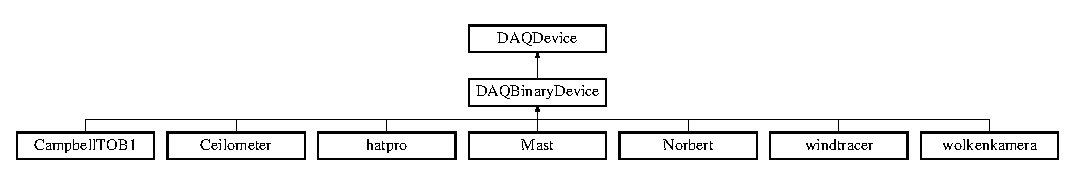
\includegraphics[height=1.920000cm]{classDAQBinaryDevice}
\end{center}
\end{figure}
\subsection*{Public Member Functions}
\begin{DoxyCompactItemize}
\item 
\hyperlink{classDAQBinaryDevice_ae8ebc9eec03d956924919ea8f91e5c56}{D\-A\-Q\-Binary\-Device} ()
\item 
\hyperlink{classDAQBinaryDevice_ad1a003d250a8fcaeec487c23fb70c479}{$\sim$\-D\-A\-Q\-Binary\-Device} ()
\item 
virtual void \hyperlink{classDAQBinaryDevice_a0169d5bde4e7841350a22793522f0529}{open\-File} ()
\item 
virtual void \hyperlink{classDAQBinaryDevice_aaa2ed58aa73772cd742d3239e21944d9}{close\-File} ()
\item 
virtual void \hyperlink{classDAQBinaryDevice_aa438886ea601984abdf2daf0f4e72543}{write\-Data} ()
\item 
virtual void \hyperlink{classDAQBinaryDevice_a725281822b7945b8c1154d079c0011ff}{read\-Data} (std\-::string full\-\_\-filename)
\end{DoxyCompactItemize}
\subsection*{Protected Attributes}
\begin{DoxyCompactItemize}
\item 
int \hyperlink{classDAQBinaryDevice_a561f25e67b72d217b904a104175f0bfd}{fd\-\_\-data}
\item 
unsigned long \hyperlink{classDAQBinaryDevice_a8eac27c83c30772d1260fda3acbde4be}{n\-Samples}
\item 
unsigned long \hyperlink{classDAQBinaryDevice_a50f33c0714edaf6468affc7200229978}{n\-Template}
\end{DoxyCompactItemize}
\subsection*{Additional Inherited Members}


\subsection{Detailed Description}
Implementation for the weather mast D\-A\-Q devices that are used for turbulence, energy balance and 20m mast. The data files contain any kind of binary format. 

\subsection{Constructor \& Destructor Documentation}
\hypertarget{classDAQBinaryDevice_ae8ebc9eec03d956924919ea8f91e5c56}{\index{D\-A\-Q\-Binary\-Device@{D\-A\-Q\-Binary\-Device}!D\-A\-Q\-Binary\-Device@{D\-A\-Q\-Binary\-Device}}
\index{D\-A\-Q\-Binary\-Device@{D\-A\-Q\-Binary\-Device}!DAQBinaryDevice@{D\-A\-Q\-Binary\-Device}}
\subsubsection[{D\-A\-Q\-Binary\-Device}]{\setlength{\rightskip}{0pt plus 5cm}D\-A\-Q\-Binary\-Device\-::\-D\-A\-Q\-Binary\-Device (
\begin{DoxyParamCaption}
{}
\end{DoxyParamCaption}
)}}\label{classDAQBinaryDevice_ae8ebc9eec03d956924919ea8f91e5c56}
\hypertarget{classDAQBinaryDevice_ad1a003d250a8fcaeec487c23fb70c479}{\index{D\-A\-Q\-Binary\-Device@{D\-A\-Q\-Binary\-Device}!$\sim$\-D\-A\-Q\-Binary\-Device@{$\sim$\-D\-A\-Q\-Binary\-Device}}
\index{$\sim$\-D\-A\-Q\-Binary\-Device@{$\sim$\-D\-A\-Q\-Binary\-Device}!DAQBinaryDevice@{D\-A\-Q\-Binary\-Device}}
\subsubsection[{$\sim$\-D\-A\-Q\-Binary\-Device}]{\setlength{\rightskip}{0pt plus 5cm}D\-A\-Q\-Binary\-Device\-::$\sim$\-D\-A\-Q\-Binary\-Device (
\begin{DoxyParamCaption}
{}
\end{DoxyParamCaption}
)}}\label{classDAQBinaryDevice_ad1a003d250a8fcaeec487c23fb70c479}


\subsection{Member Function Documentation}
\hypertarget{classDAQBinaryDevice_aaa2ed58aa73772cd742d3239e21944d9}{\index{D\-A\-Q\-Binary\-Device@{D\-A\-Q\-Binary\-Device}!close\-File@{close\-File}}
\index{close\-File@{close\-File}!DAQBinaryDevice@{D\-A\-Q\-Binary\-Device}}
\subsubsection[{close\-File}]{\setlength{\rightskip}{0pt plus 5cm}void D\-A\-Q\-Binary\-Device\-::close\-File (
\begin{DoxyParamCaption}
{}
\end{DoxyParamCaption}
)\hspace{0.3cm}{\ttfamily [virtual]}}}\label{classDAQBinaryDevice_aaa2ed58aa73772cd742d3239e21944d9}
Close file for reading 

Reimplemented from \hyperlink{classDAQDevice_ae27c5729563be895c0d0a607ee023e30}{D\-A\-Q\-Device}.

\hypertarget{classDAQBinaryDevice_a0169d5bde4e7841350a22793522f0529}{\index{D\-A\-Q\-Binary\-Device@{D\-A\-Q\-Binary\-Device}!open\-File@{open\-File}}
\index{open\-File@{open\-File}!DAQBinaryDevice@{D\-A\-Q\-Binary\-Device}}
\subsubsection[{open\-File}]{\setlength{\rightskip}{0pt plus 5cm}void D\-A\-Q\-Binary\-Device\-::open\-File (
\begin{DoxyParamCaption}
{}
\end{DoxyParamCaption}
)\hspace{0.3cm}{\ttfamily [virtual]}}}\label{classDAQBinaryDevice_a0169d5bde4e7841350a22793522f0529}
Open file for writing data 

Reimplemented from \hyperlink{classDAQDevice_a6631b33164c86e7da8d0cd7eca50863f}{D\-A\-Q\-Device}.

\hypertarget{classDAQBinaryDevice_a725281822b7945b8c1154d079c0011ff}{\index{D\-A\-Q\-Binary\-Device@{D\-A\-Q\-Binary\-Device}!read\-Data@{read\-Data}}
\index{read\-Data@{read\-Data}!DAQBinaryDevice@{D\-A\-Q\-Binary\-Device}}
\subsubsection[{read\-Data}]{\setlength{\rightskip}{0pt plus 5cm}void D\-A\-Q\-Binary\-Device\-::read\-Data (
\begin{DoxyParamCaption}
\item[{std\-::string}]{full\-\_\-filename}
\end{DoxyParamCaption}
)\hspace{0.3cm}{\ttfamily [virtual]}}}\label{classDAQBinaryDevice_a725281822b7945b8c1154d079c0011ff}


Reimplemented from \hyperlink{classDAQDevice_a218267a0239e980d418ee5ab70f884e7}{D\-A\-Q\-Device}.



Reimplemented in \hyperlink{classwindtracer_a3017c180cdd51ab93c5b73c2f84059f5}{windtracer}, \hyperlink{classNorbert_a0b1b1ba6fc63b8662a537c66815ff19b}{Norbert}, \hyperlink{classCeilometer_a9ef73907ba808f6f967b32dc3a161a66}{Ceilometer}, \hyperlink{classwolkenkamera_a9d63655c35a98dec0583b27a67b292ce}{wolkenkamera}, and \hyperlink{classhatpro_a6a22e73eb5d50f6425d8e46795d2007a}{hatpro}.

\hypertarget{classDAQBinaryDevice_aa438886ea601984abdf2daf0f4e72543}{\index{D\-A\-Q\-Binary\-Device@{D\-A\-Q\-Binary\-Device}!write\-Data@{write\-Data}}
\index{write\-Data@{write\-Data}!DAQBinaryDevice@{D\-A\-Q\-Binary\-Device}}
\subsubsection[{write\-Data}]{\setlength{\rightskip}{0pt plus 5cm}void D\-A\-Q\-Binary\-Device\-::write\-Data (
\begin{DoxyParamCaption}
{}
\end{DoxyParamCaption}
)\hspace{0.3cm}{\ttfamily [virtual]}}}\label{classDAQBinaryDevice_aa438886ea601984abdf2daf0f4e72543}
Write simulated data set 

Reimplemented from \hyperlink{classDAQDevice_acdc9d3765b1dfd845f99ec9c93071811}{D\-A\-Q\-Device}.



\subsection{Member Data Documentation}
\hypertarget{classDAQBinaryDevice_a561f25e67b72d217b904a104175f0bfd}{\index{D\-A\-Q\-Binary\-Device@{D\-A\-Q\-Binary\-Device}!fd\-\_\-data@{fd\-\_\-data}}
\index{fd\-\_\-data@{fd\-\_\-data}!DAQBinaryDevice@{D\-A\-Q\-Binary\-Device}}
\subsubsection[{fd\-\_\-data}]{\setlength{\rightskip}{0pt plus 5cm}int D\-A\-Q\-Binary\-Device\-::fd\-\_\-data\hspace{0.3cm}{\ttfamily [protected]}}}\label{classDAQBinaryDevice_a561f25e67b72d217b904a104175f0bfd}
File descriptor for reading binary data files \hypertarget{classDAQBinaryDevice_a8eac27c83c30772d1260fda3acbde4be}{\index{D\-A\-Q\-Binary\-Device@{D\-A\-Q\-Binary\-Device}!n\-Samples@{n\-Samples}}
\index{n\-Samples@{n\-Samples}!DAQBinaryDevice@{D\-A\-Q\-Binary\-Device}}
\subsubsection[{n\-Samples}]{\setlength{\rightskip}{0pt plus 5cm}unsigned long D\-A\-Q\-Binary\-Device\-::n\-Samples\hspace{0.3cm}{\ttfamily [protected]}}}\label{classDAQBinaryDevice_a8eac27c83c30772d1260fda3acbde4be}
Number of samples written by \hyperlink{classDAQBinaryDevice_aa438886ea601984abdf2daf0f4e72543}{write\-Data()} \hypertarget{classDAQBinaryDevice_a50f33c0714edaf6468affc7200229978}{\index{D\-A\-Q\-Binary\-Device@{D\-A\-Q\-Binary\-Device}!n\-Template@{n\-Template}}
\index{n\-Template@{n\-Template}!DAQBinaryDevice@{D\-A\-Q\-Binary\-Device}}
\subsubsection[{n\-Template}]{\setlength{\rightskip}{0pt plus 5cm}unsigned long D\-A\-Q\-Binary\-Device\-::n\-Template\hspace{0.3cm}{\ttfamily [protected]}}}\label{classDAQBinaryDevice_a50f33c0714edaf6468affc7200229978}
Number of the current data set in the template file used by \hyperlink{classDAQBinaryDevice_aa438886ea601984abdf2daf0f4e72543}{write\-Data()} 

The documentation for this class was generated from the following files\-:\begin{DoxyCompactItemize}
\item 
/home/ntj/\-Development/phd/kitcube-\/tools/src/kitcube-\/devices/\hyperlink{daqbinarydevice_8h}{daqbinarydevice.\-h}\item 
/home/ntj/\-Development/phd/kitcube-\/tools/src/kitcube-\/devices/\hyperlink{daqbinarydevice_8cpp}{daqbinarydevice.\-cpp}\end{DoxyCompactItemize}

\hypertarget{classDAQDevice}{\section{D\-A\-Q\-Device Class Reference}
\label{classDAQDevice}\index{D\-A\-Q\-Device@{D\-A\-Q\-Device}}
}


{\ttfamily \#include $<$daqdevice.\-h$>$}

Inheritance diagram for D\-A\-Q\-Device\-:\begin{figure}[H]
\begin{center}
\leavevmode
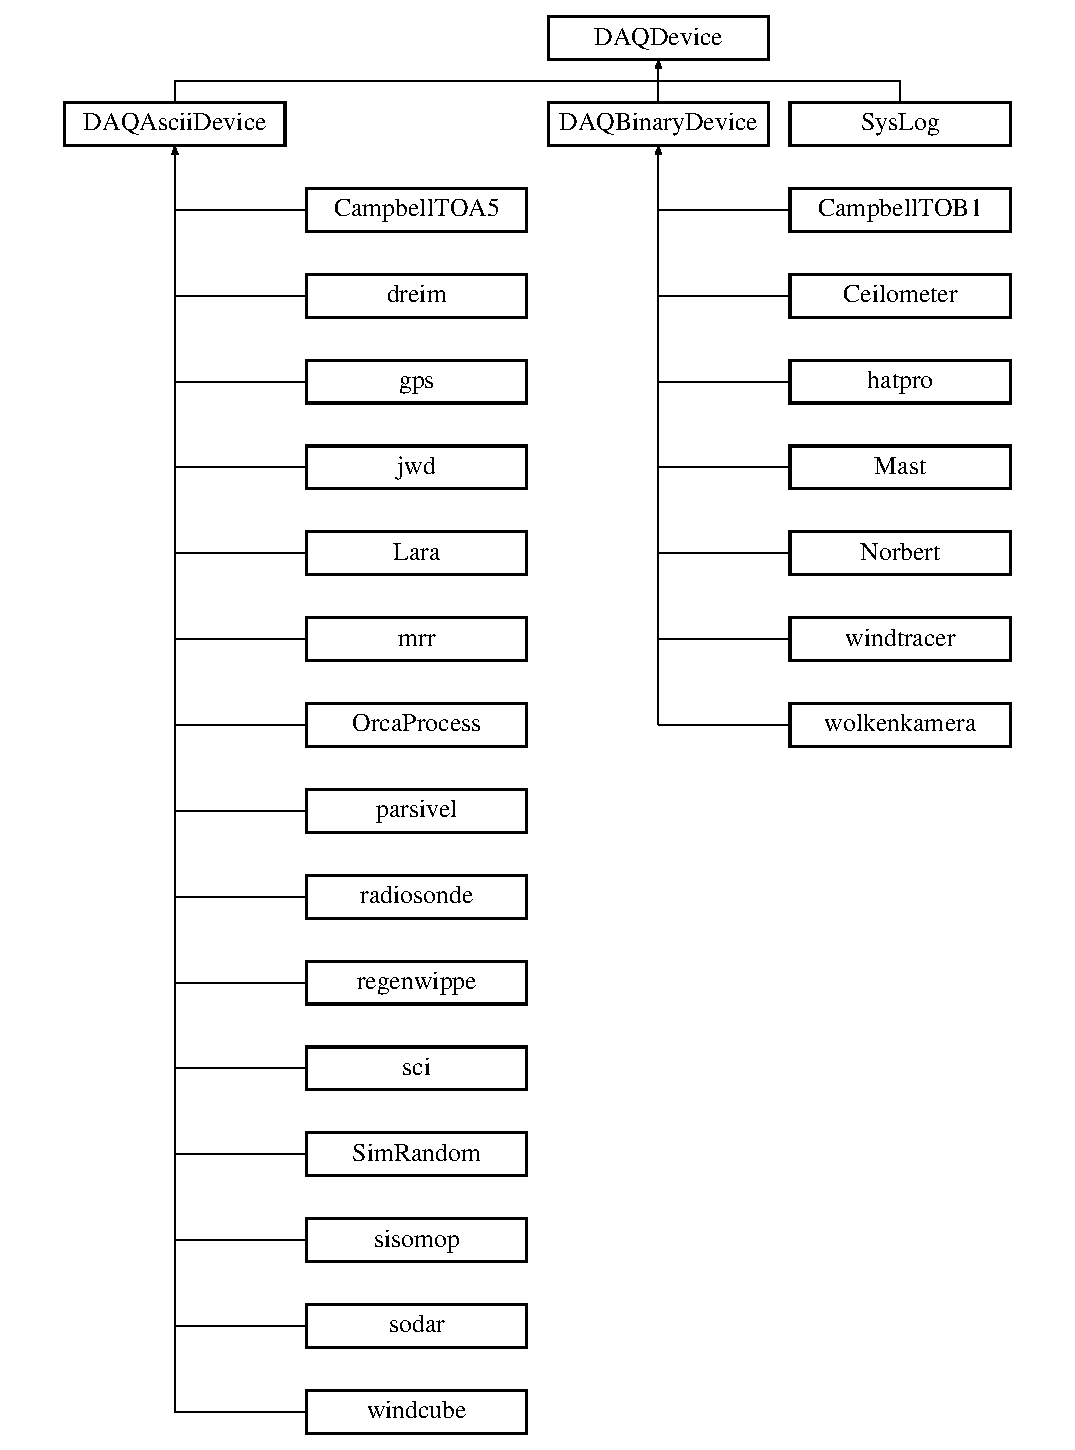
\includegraphics[height=12.000000cm]{classDAQDevice}
\end{center}
\end{figure}
\subsection*{Public Member Functions}
\begin{DoxyCompactItemize}
\item 
\hyperlink{classDAQDevice_adcc18d71d95de6d875f99894383092f6}{D\-A\-Q\-Device} ()
\item 
virtual \hyperlink{classDAQDevice_a2fb9f1fe7ff9496d52654bda6b1a099b}{$\sim$\-D\-A\-Q\-Device} ()
\item 
int \hyperlink{classDAQDevice_aa077dc208e0af098a95c75a97dcb4a16}{get\-N\-Sensors} ()
\item 
virtual void \hyperlink{classDAQDevice_a7685cec80865752cc0ef3ab49c6c2277}{set\-Config\-Defaults} ()
\item 
void \hyperlink{classDAQDevice_aedf0ba7667fd7e0952f04878af2d3bb4}{read\-Inifile\-Common} (const char $\ast$\hyperlink{classDAQDevice_aeacc409b639f3ed09cfdbd9b2c3e7d09}{inifile})
\item 
virtual void \hyperlink{classDAQDevice_a47c1cf880beb17950a575168274bc213}{read\-Inifile} (const char $\ast$\hyperlink{classDAQDevice_aeacc409b639f3ed09cfdbd9b2c3e7d09}{inifile}, const char $\ast$group=0)
\item 
void \hyperlink{classDAQDevice_ac1fa63e8be022587c80af60a67fb0893}{read\-Axis} (const char $\ast$\hyperlink{classDAQDevice_aeacc409b639f3ed09cfdbd9b2c3e7d09}{inifile})
\item 
void \hyperlink{classDAQDevice_adb56a07d66555732a901196519b1b963}{get\-Sensor\-Names} (const char $\ast$sensor\-\_\-list\-\_\-file\-\_\-name)
\item 
void \hyperlink{classDAQDevice_aee072d124ed6eb99003d24233f3eb5f6}{get\-Sampling\-Time} (struct timeval $\ast$time)
\item 
void \hyperlink{classDAQDevice_a6351102955977889363de75de88436f2}{get\-Last\-Timestamp} (struct timeval $\ast$time)
\item 
void \hyperlink{classDAQDevice_ae8c54de957f24848f9882d427ccda1f1}{get\-Next\-Timestamp} (struct timeval $\ast$time)
\item 
void \hyperlink{classDAQDevice_afc9b0a86f2c4d7a2dbf099d8eebade23}{set\-Last\-Timestamp} (struct timeval $\ast$time)
\item 
void \hyperlink{classDAQDevice_add887304744674aae4d21b9988437dc5}{create\-Directories} (const char $\ast$\hyperlink{classDAQDevice_a388a037825fdd2248eb1cadf15780bcd}{path})
\item 
virtual void \hyperlink{classDAQDevice_aa31998fc15327f4999946adcdbb9f770}{open\-File} (const char $\ast$filenname)
\item 
virtual void \hyperlink{classDAQDevice_a6631b33164c86e7da8d0cd7eca50863f}{open\-File} ()
\item 
virtual void \hyperlink{classDAQDevice_a0626e224d6263cca633f74b0aae65223}{open\-New\-File} ()
\item 
virtual void \hyperlink{classDAQDevice_ae27c5729563be895c0d0a607ee023e30}{close\-File} ()
\item 
const char $\ast$ \hyperlink{classDAQDevice_a45f86e1db8a54d14559ad4f74078a49e}{get\-Archive\-Dir} ()
\item 
virtual const char $\ast$ \hyperlink{classDAQDevice_a7d7d41f0c1496221e589d84b38d1c865}{get\-Data\-Dir} ()
\item 
virtual const char $\ast$ \hyperlink{classDAQDevice_af4734900eb86417b3160a723a077f8f5}{get\-Data\-Filename} ()
\item 
virtual void \hyperlink{classDAQDevice_a32f118d291f1c7b8fe47a16474b825e2}{open\-Database} ()
\item 
void \hyperlink{classDAQDevice_a88a9330a2982674e6e9097790c7e65cb}{open\-Status\-Tab} ()
\item 
void \hyperlink{classDAQDevice_adc401ccdc283c2121a8ef0f5fe67f543}{connect\-Database} ()
\item 
virtual int \hyperlink{classDAQDevice_ac4867b7e5aff2d5c404d6eb1053dda71}{create\-\_\-data\-\_\-table} ()
\item 
virtual void \hyperlink{classDAQDevice_a00f5a8af6622bc8aebcf930f2ae674ac}{close\-Database} ()
\item 
virtual int \hyperlink{classDAQDevice_af5fa373af9a089c18c7fd1d662db144f}{read\-Header} (const char $\ast$header)
\item 
virtual void \hyperlink{classDAQDevice_ac663fe98e445fc57df55dac84a2c9846}{read\-Header} ()
\item 
virtual void \hyperlink{classDAQDevice_aad39c13f039abd6e6a9b0aa21a7c8a4d}{write\-Header} ()
\item 
virtual int \hyperlink{classDAQDevice_a37f6fcab4893285e7f7d74670294a645}{parse\-Data} (char $\ast$line, struct timeval $\ast$l\-\_\-t\-Data, double $\ast$\hyperlink{classDAQDevice_ad148188c57598fdf4fd4c1c333aeb0d8}{sensor\-Value})
\item 
void \hyperlink{classDAQDevice_a3c31d33d7af79b99cc86dc00554e9472}{register\-Status\-Tab} (const char $\ast$status=0, const char $\ast$comment=0)
\item 
virtual void \hyperlink{classDAQDevice_a5262fc7b919829bc439e9eebfc8592e7}{store\-Sensor\-Data} ()
\item 
virtual void \hyperlink{classDAQDevice_a218267a0239e980d418ee5ab70f884e7}{read\-Data} (std\-::string full\-\_\-filename)
\item 
virtual void \hyperlink{classDAQDevice_a06d18d7b372d35c55f8a1a399f582a94}{update\-Data\-Set} (unsigned char $\ast$buf)
\item 
virtual void \hyperlink{classDAQDevice_acdc9d3765b1dfd845f99ec9c93071811}{write\-Data} ()
\item 
virtual long \hyperlink{classDAQDevice_a56a712062b2b17c6a73cb7fb0a475d2e}{get\-File\-Number} (char $\ast$\hyperlink{classDAQDevice_a7f9cda7cf5b41f6b134c313477e9644b}{filename})
\item 
void \hyperlink{classDAQDevice_a8d52a03c722baf86c7279478f31f6e60}{get\-New\-Files} (const char $\ast$dir=0)
\item 
unsigned int \hyperlink{classDAQDevice_ae96988af5ad52d284d3d10dc7e52c351}{get\-Module\-Number} ()
\item 
virtual unsigned int \hyperlink{classDAQDevice_a61d08492a11c30944dfaf3b86115abe8}{get\-Sensor\-Group} ()
\item 
unsigned long \hyperlink{classDAQDevice_a9bc65c78b7855fc29bf80e1dae950109}{get\-Timestamp} (const char $\ast$date, const char $\ast$time)
\item 
void \hyperlink{classDAQDevice_ad62233d33b79371db16f666864fbc83b}{set\-Debug\-Level} (int level)
\item 
virtual void \hyperlink{classDAQDevice_a42934eca41ab337dc5874e9e70ba1fab}{set\-App\-Id} (int id)
\item 
int \hyperlink{classDAQDevice_a176d88638d40c00284fe465344f76f32}{get\-App\-Id} ()
\item 
bool \hyperlink{classDAQDevice_a56426722a8c4ee14d242fd15b49440c5}{reached\-E\-O\-F} ()
\item 
unsigned int \hyperlink{classDAQDevice_a873db9cbaef6c48fb42bbcd4e3d5dc3b}{get\-Processed\-Data} ()
\item 
void \hyperlink{classDAQDevice_acf52574e463497c82a7435190710d198}{save\-File\-Position} (long last\-Index, unsigned long curr\-Pos, struct timeval \&timestamp)
\item 
void \hyperlink{classDAQDevice_a315931693c343f5d6f9b607d406e25ac}{load\-File\-Position} (long \&last\-Index, unsigned long \&last\-Pos, struct timeval \&timestamp)
\item 
void \hyperlink{classDAQDevice_a8aab00baa4f0f0b5718e88539b3d3479}{reset\-File\-Position} ()
\end{DoxyCompactItemize}
\subsection*{Public Attributes}
\begin{DoxyCompactItemize}
\item 
std\-::string \hyperlink{classDAQDevice_aab515711e872a4ee38ae5b1278f64286}{sensor\-Listfile}
\end{DoxyCompactItemize}
\subsection*{Protected Member Functions}
\begin{DoxyCompactItemize}
\item 
void \hyperlink{classDAQDevice_a66f31f8b094adaa54a79fd28730248d6}{load\-Python} ()
\item 
void \hyperlink{classDAQDevice_aaebe17251aead6111efcb7bcb3006c60}{release\-Python} ()
\item 
void \hyperlink{classDAQDevice_a63bf061ad2297861e1e8d8144445235e}{read\-Data\-With\-Python} (const char $\ast$\hyperlink{classDAQDevice_a7f9cda7cf5b41f6b134c313477e9644b}{filename}, double $\ast$\hyperlink{classDAQDevice_ad148188c57598fdf4fd4c1c333aeb0d8}{sensor\-Value})
\item 
virtual int \hyperlink{classDAQDevice_add621117663b1aa2b3c3efcc115a8126}{create\-\_\-data\-\_\-table\-\_\-name} (std\-::string \&data\-\_\-table\-\_\-name)
\item 
int \hyperlink{classDAQDevice_acd12b71320ddcf9c875df0cb701cd581}{read\-\_\-ascii\-\_\-line} (char $\ast$$\ast$\hyperlink{classDAQDevice_ab661aa5c5b4bafe78354f5169b1c7d2f}{buffer}, size\-\_\-t $\ast$length, F\-I\-L\-E $\ast$file\-\_\-ptr)
\end{DoxyCompactItemize}
\subsection*{Protected Attributes}
\begin{DoxyCompactItemize}
\item 
bool \hyperlink{classDAQDevice_ad9f21827cf4471e11b5e5bfe8f29152f}{reset}
\item 
bool \hyperlink{classDAQDevice_a6103f8804ccb23ac0e76e38ed954ddbc}{use\-Ticks}
\item 
int \hyperlink{classDAQDevice_a91b1652c6ca593eaf3f04e3118cd2420}{len\-Header}
\item 
int \hyperlink{classDAQDevice_a155e6dba34521962283c83f1bda63799}{len\-Header\-Lines}
\item 
int \hyperlink{classDAQDevice_ae6cf89824f15528d92fe1e31b2dacf59}{len\-Data\-Set}
\item 
int \hyperlink{classDAQDevice_af1607d0a9cdd02c6dfe9a7db01fbe4e8}{no\-Data}
\item 
int \hyperlink{classDAQDevice_aae80d100e6407da492b7bda911739bb8}{t\-Sample}
\item 
struct timeval \hyperlink{classDAQDevice_a7c0d73d39b13231c2760b0aa6724b42c}{t\-Last\-Data}
\item 
int \hyperlink{classDAQDevice_a508ad6a95eec7efc47047b056f145a9d}{t\-Alarm}
\item 
int \hyperlink{classDAQDevice_a9e0cb352d0412ec6cc600cc86aee69b8}{n\-Axis}
\item 
struct \hyperlink{structaxisDef}{axis\-Def} $\ast$ \hyperlink{classDAQDevice_ad4d9fa4d5ec7b391260d89393ed13a37}{axis}
\item 
int \hyperlink{classDAQDevice_a66af3e902896059a53f5cfb2fa04e0f5}{n\-Sensors}
\item 
int \hyperlink{classDAQDevice_a308e077b2ecaff2aa04e3dec7387751a}{n\-Sensor\-Cols}
\item 
int \hyperlink{classDAQDevice_a5da19e281fb55786ad815c0d98a0c616}{profile\-\_\-length}
\item 
struct \hyperlink{structsensorType}{sensor\-Type} $\ast$ \hyperlink{classDAQDevice_a62c5391079563bbd24ac2f7cdd210710}{sensor}
\item 
struct timeval \hyperlink{classDAQDevice_af7da14a199a793fd63db3af2b2a78d92}{t\-Data}
\item 
float $\ast$ \hyperlink{classDAQDevice_ad148188c57598fdf4fd4c1c333aeb0d8}{sensor\-Value}
\item 
unsigned int \hyperlink{classDAQDevice_a4ba9ed1e61cf39c3e3eab37e8cfc908c}{processed\-Data}
\item 
F\-I\-L\-E $\ast$ \hyperlink{classDAQDevice_a0dcbda57c0b7b95d27a53ed5e1fabf59}{fdata}
\item 
unsigned long \hyperlink{classDAQDevice_a68a1e79d4d2efd8592d566bacc1838f2}{file\-Index}
\item 
int \hyperlink{classDAQDevice_a96c5b196a01603f4b8e37c3840597295}{n\-Line}
\item 
int \hyperlink{classDAQDevice_a2f0b3d2e531be7f5d06f47a4753d35bd}{app\-Id}
\item 
bool \hyperlink{classDAQDevice_a4431ebea220a683acb12ce0f78e87927}{is\-Flat\-Folder}
\item 
std\-::string \hyperlink{classDAQDevice_a2febc34bb56a8b39d0d13523ccc60c3e}{project}
\item 
std\-::string \hyperlink{classDAQDevice_a43ebbf069d065fdafba9aa9664ab76b1}{filename\-Marker}
\item 
std\-::string \hyperlink{classDAQDevice_aeacc409b639f3ed09cfdbd9b2c3e7d09}{inifile}
\item 
std\-::string \hyperlink{classDAQDevice_a10e5184e28ccafa407167c032f8496ea}{ini\-Group}
\item 
std\-::string \hyperlink{classDAQDevice_a388a037825fdd2248eb1cadf15780bcd}{path}
\item 
std\-::string \hyperlink{classDAQDevice_a7f9cda7cf5b41f6b134c313477e9644b}{filename}
\item 
std\-::string \hyperlink{classDAQDevice_a1bb9bdd8a55337b40e44d159cb1cc8e5}{full\-Filename}
\item 
std\-::string \hyperlink{classDAQDevice_a5fb94d0eed52bfb5df51424a21f3482f}{module\-Name}
\item 
std\-::string \hyperlink{classDAQDevice_a962a90d4dd66bb3d4c3cab6ec628db73}{module\-Comment}
\item 
std\-::string \hyperlink{classDAQDevice_ab246fcff5cbe2a1f4748db00bb9fa5c4}{module\-Type}
\item 
unsigned int \hyperlink{classDAQDevice_a07fc449a690016ffa1b1bc029b956c02}{module\-Number}
\item 
std\-::string \hyperlink{classDAQDevice_a8adec9c21ffa22beee97e2eda1f2488c}{data\-Sub\-Dir}
\item 
std\-::string \hyperlink{classDAQDevice_a63a6793abe5933e7dc71cd673bd0f98f}{sensor\-Group}
\item 
unsigned int \hyperlink{classDAQDevice_aa35abc3d365a36659b64df6cadf2c807}{sensor\-Group\-Number}
\item 
int \hyperlink{classDAQDevice_a06e7f707d2d97b192a4389a0c4fd231d}{header\-Line}
\item 
std\-::string \hyperlink{classDAQDevice_ae8e11658c72f3a6468cc37f1e8cf08bb}{data\-Sep}
\item 
std\-::string \hyperlink{classDAQDevice_af34a3a4a6cc3b4a8c01ce42d495be6c2}{comment\-Char}
\item 
std\-::string \hyperlink{classDAQDevice_a35f89e6ada8acd69ce9b705633370345}{timestamp\-Format}
\item 
std\-::string \hyperlink{classDAQDevice_a1fcd353aea74e51801b36d5728f67e66}{config\-Dir}
\item 
std\-::string \hyperlink{classDAQDevice_a6df191f01fd268b0072e09ba2b76827f}{remote\-Dir}
\item 
std\-::string \hyperlink{classDAQDevice_a40eb0f06fac7ec90ed04b766b1f5df3c}{archive\-Dir}
\item 
std\-::string \hyperlink{classDAQDevice_ae99e0e25b09c03713caac3f9b2baaee8}{data\-Dir}
\item 
std\-::string \hyperlink{classDAQDevice_ad3cde27a8f45ea3af4495a9d366c31c3}{datafile\-Mask}
\item 
std\-::string \hyperlink{classDAQDevice_a3d221f2cd6d5d903cbaa8c80abe495de}{datafile\-Index\-Format}
\item 
std\-::string \hyperlink{classDAQDevice_a551a005ad3f98c83a2b8b38bc3634007}{datafile\-Template}
\item 
std\-::string \hyperlink{classDAQDevice_ae6db34954e8c3723feba1d32a7643095}{rsync\-Args}
\item 
int \hyperlink{classDAQDevice_ad0a7f34f8a98c28fa5660714c048e657}{init\-Done}
\item 
std\-::string \hyperlink{classDAQDevice_ac06e9cd93e95a3c4e33970edb79f9148}{compression\-Type}
\item 
std\-::string \hyperlink{classDAQDevice_ad85b8bb5afbe0a9c3cd75e7ee9ef83ee}{db\-Host}
\item 
int \hyperlink{classDAQDevice_a275b8a01d1219d64a64a2536038039a4}{db\-Port}
\item 
std\-::string \hyperlink{classDAQDevice_afb3d256eedb538510939b8c40e26a968}{db\-Name}
\item 
std\-::string \hyperlink{classDAQDevice_a1cecb55a4edaf4299411f650c7410e5e}{db\-User}
\item 
std\-::string \hyperlink{classDAQDevice_ab02618ceb308d39d365bc0b394914b69}{db\-Password}
\item 
std\-::string \hyperlink{classDAQDevice_a4140887251923bc9715a23fb63849785}{sensor\-Table\-Name}
\item 
std\-::string \hyperlink{classDAQDevice_af33c38b4bf6c138dc60d84a9bfb6df85}{axis\-Table\-Name}
\item 
std\-::string \hyperlink{classDAQDevice_a0061ca1e9e172bc2cb113a6f6b7f0ade}{module\-Table\-Name}
\item 
std\-::string \hyperlink{classDAQDevice_a3b932e09b546454324cc07d7958f58ac}{data\-Table\-Name}
\item 
std\-::string \hyperlink{classDAQDevice_ac2ae1cde05bf5d13d18e213c94c5dadc}{data\-Table\-Prefix}
\item 
std\-::string \hyperlink{classDAQDevice_a9e039294e443228fc1854ec798d1b5c4}{status\-Table\-Name}
\item 
std\-::string \hyperlink{classDAQDevice_a1d817232e36e532fbed88e7013e30567}{status\-Table\-Key}
\item 
std\-::string \hyperlink{classDAQDevice_a4d916c2296ae785dbe02859721b410e6}{python\-Dir}
\item 
std\-::string \hyperlink{classDAQDevice_a75b36464a8009089f1f5721764f7bf70}{python\-Module}
\item 
std\-::string \hyperlink{classDAQDevice_ac2662dfe78ec08ab4bd8cc8e159fed0f}{python\-Function}
\item 
int \hyperlink{classDAQDevice_ae7b23729ae0dc7ab3cd0e4c633bf4e25}{debug}
\item 
std\-::string \hyperlink{classDAQDevice_ab661aa5c5b4bafe78354f5169b1c7d2f}{buffer}
\item 
bool \hyperlink{classDAQDevice_a0adfd30435b899ce439998bbdd3dae91}{fd\-\_\-eof}
\end{DoxyCompactItemize}
\subsection*{Private Member Functions}
\begin{DoxyCompactItemize}
\item 
int \hyperlink{classDAQDevice_ac3c405fb5cc77a22c450b952ae6b82f3}{get\-\_\-file\-\_\-list} (std\-::string directory)
\end{DoxyCompactItemize}
\subsection*{Private Attributes}
\begin{DoxyCompactItemize}
\item 
std\-::string \hyperlink{classDAQDevice_a2abc939adabdc9bc9a88bd1db5dcfd08}{filename\-Tmpl}
\item 
std\-::string \hyperlink{classDAQDevice_add8342b70f7350c0d8b7bf4ba3e9c5b4}{basedir}
\item 
std\-::string \hyperlink{classDAQDevice_a6dc47f2c1a792f5a1ed09b03ac98e8cc}{basedir\-Tmpl}
\item 
std\-::string \hyperlink{classDAQDevice_aab09bfdbb1d0aa4b413e4bbbc5e3c5a6}{location}
\item 
std\-::map$<$ long, std\-::string $>$ \hyperlink{classDAQDevice_a962745a4a4f20898c918d59fabf05e2a}{dateien}
\end{DoxyCompactItemize}


\subsection{Detailed Description}
Implementation for the weather mast D\-A\-Q devices that are used for turbulence, energy balance and 20m mast. 

\subsection{Constructor \& Destructor Documentation}
\hypertarget{classDAQDevice_adcc18d71d95de6d875f99894383092f6}{\index{D\-A\-Q\-Device@{D\-A\-Q\-Device}!D\-A\-Q\-Device@{D\-A\-Q\-Device}}
\index{D\-A\-Q\-Device@{D\-A\-Q\-Device}!DAQDevice@{D\-A\-Q\-Device}}
\subsubsection[{D\-A\-Q\-Device}]{\setlength{\rightskip}{0pt plus 5cm}D\-A\-Q\-Device\-::\-D\-A\-Q\-Device (
\begin{DoxyParamCaption}
{}
\end{DoxyParamCaption}
)}}\label{classDAQDevice_adcc18d71d95de6d875f99894383092f6}
\hypertarget{classDAQDevice_a2fb9f1fe7ff9496d52654bda6b1a099b}{\index{D\-A\-Q\-Device@{D\-A\-Q\-Device}!$\sim$\-D\-A\-Q\-Device@{$\sim$\-D\-A\-Q\-Device}}
\index{$\sim$\-D\-A\-Q\-Device@{$\sim$\-D\-A\-Q\-Device}!DAQDevice@{D\-A\-Q\-Device}}
\subsubsection[{$\sim$\-D\-A\-Q\-Device}]{\setlength{\rightskip}{0pt plus 5cm}D\-A\-Q\-Device\-::$\sim$\-D\-A\-Q\-Device (
\begin{DoxyParamCaption}
{}
\end{DoxyParamCaption}
)\hspace{0.3cm}{\ttfamily [virtual]}}}\label{classDAQDevice_a2fb9f1fe7ff9496d52654bda6b1a099b}


\subsection{Member Function Documentation}
\hypertarget{classDAQDevice_a00f5a8af6622bc8aebcf930f2ae674ac}{\index{D\-A\-Q\-Device@{D\-A\-Q\-Device}!close\-Database@{close\-Database}}
\index{close\-Database@{close\-Database}!DAQDevice@{D\-A\-Q\-Device}}
\subsubsection[{close\-Database}]{\setlength{\rightskip}{0pt plus 5cm}void D\-A\-Q\-Device\-::close\-Database (
\begin{DoxyParamCaption}
{}
\end{DoxyParamCaption}
)\hspace{0.3cm}{\ttfamily [virtual]}}}\label{classDAQDevice_a00f5a8af6622bc8aebcf930f2ae674ac}
\hypertarget{classDAQDevice_ae27c5729563be895c0d0a607ee023e30}{\index{D\-A\-Q\-Device@{D\-A\-Q\-Device}!close\-File@{close\-File}}
\index{close\-File@{close\-File}!DAQDevice@{D\-A\-Q\-Device}}
\subsubsection[{close\-File}]{\setlength{\rightskip}{0pt plus 5cm}void D\-A\-Q\-Device\-::close\-File (
\begin{DoxyParamCaption}
{}
\end{DoxyParamCaption}
)\hspace{0.3cm}{\ttfamily [virtual]}}}\label{classDAQDevice_ae27c5729563be895c0d0a607ee023e30}


Reimplemented in \hyperlink{classDAQBinaryDevice_aaa2ed58aa73772cd742d3239e21944d9}{D\-A\-Q\-Binary\-Device}, and \hyperlink{classDAQAsciiDevice_aef686b204dd3569291c5cc4534f7aa24}{D\-A\-Q\-Ascii\-Device}.

\hypertarget{classDAQDevice_adc401ccdc283c2121a8ef0f5fe67f543}{\index{D\-A\-Q\-Device@{D\-A\-Q\-Device}!connect\-Database@{connect\-Database}}
\index{connect\-Database@{connect\-Database}!DAQDevice@{D\-A\-Q\-Device}}
\subsubsection[{connect\-Database}]{\setlength{\rightskip}{0pt plus 5cm}void D\-A\-Q\-Device\-::connect\-Database (
\begin{DoxyParamCaption}
{}
\end{DoxyParamCaption}
)}}\label{classDAQDevice_adc401ccdc283c2121a8ef0f5fe67f543}
Connect to the database \char`\"{}$<$project$>$\-\_\-active\char`\"{}. The database is created, if not existing. The function is included from \hyperlink{classDAQDevice_a32f118d291f1c7b8fe47a16474b825e2}{open\-Database()}. \hypertarget{classDAQDevice_ac4867b7e5aff2d5c404d6eb1053dda71}{\index{D\-A\-Q\-Device@{D\-A\-Q\-Device}!create\-\_\-data\-\_\-table@{create\-\_\-data\-\_\-table}}
\index{create\-\_\-data\-\_\-table@{create\-\_\-data\-\_\-table}!DAQDevice@{D\-A\-Q\-Device}}
\subsubsection[{create\-\_\-data\-\_\-table}]{\setlength{\rightskip}{0pt plus 5cm}int D\-A\-Q\-Device\-::create\-\_\-data\-\_\-table (
\begin{DoxyParamCaption}
{}
\end{DoxyParamCaption}
)\hspace{0.3cm}{\ttfamily [virtual]}}}\label{classDAQDevice_ac4867b7e5aff2d5c404d6eb1053dda71}
Create data table, if it doesn't exist. The function is called by \hyperlink{classDAQDevice_a32f118d291f1c7b8fe47a16474b825e2}{open\-Database()}. 

Reimplemented in \hyperlink{classwindtracer_a4921e9eaa0f568b3119bd8f253484388}{windtracer}, \hyperlink{classsodar_afcdf95cbd5488e8a68d15d0817b62ba6}{sodar}, and \hyperlink{classhatpro_aa252764179bbe6f3c06b4a02ded7be52}{hatpro}.

\hypertarget{classDAQDevice_add621117663b1aa2b3c3efcc115a8126}{\index{D\-A\-Q\-Device@{D\-A\-Q\-Device}!create\-\_\-data\-\_\-table\-\_\-name@{create\-\_\-data\-\_\-table\-\_\-name}}
\index{create\-\_\-data\-\_\-table\-\_\-name@{create\-\_\-data\-\_\-table\-\_\-name}!DAQDevice@{D\-A\-Q\-Device}}
\subsubsection[{create\-\_\-data\-\_\-table\-\_\-name}]{\setlength{\rightskip}{0pt plus 5cm}int D\-A\-Q\-Device\-::create\-\_\-data\-\_\-table\-\_\-name (
\begin{DoxyParamCaption}
\item[{std\-::string \&}]{data\-\_\-table\-\_\-name}
\end{DoxyParamCaption}
)\hspace{0.3cm}{\ttfamily [protected]}, {\ttfamily [virtual]}}}\label{classDAQDevice_add621117663b1aa2b3c3efcc115a8126}


Reimplemented in \hyperlink{classwindtracer_af9d739964c034029c99e283a283b506f}{windtracer}.

\hypertarget{classDAQDevice_add887304744674aae4d21b9988437dc5}{\index{D\-A\-Q\-Device@{D\-A\-Q\-Device}!create\-Directories@{create\-Directories}}
\index{create\-Directories@{create\-Directories}!DAQDevice@{D\-A\-Q\-Device}}
\subsubsection[{create\-Directories}]{\setlength{\rightskip}{0pt plus 5cm}void D\-A\-Q\-Device\-::create\-Directories (
\begin{DoxyParamCaption}
\item[{const char $\ast$}]{path}
\end{DoxyParamCaption}
)}}\label{classDAQDevice_add887304744674aae4d21b9988437dc5}
\hypertarget{classDAQDevice_ac3c405fb5cc77a22c450b952ae6b82f3}{\index{D\-A\-Q\-Device@{D\-A\-Q\-Device}!get\-\_\-file\-\_\-list@{get\-\_\-file\-\_\-list}}
\index{get\-\_\-file\-\_\-list@{get\-\_\-file\-\_\-list}!DAQDevice@{D\-A\-Q\-Device}}
\subsubsection[{get\-\_\-file\-\_\-list}]{\setlength{\rightskip}{0pt plus 5cm}int D\-A\-Q\-Device\-::get\-\_\-file\-\_\-list (
\begin{DoxyParamCaption}
\item[{std\-::string}]{directory}
\end{DoxyParamCaption}
)\hspace{0.3cm}{\ttfamily [private]}}}\label{classDAQDevice_ac3c405fb5cc77a22c450b952ae6b82f3}
\hypertarget{classDAQDevice_a176d88638d40c00284fe465344f76f32}{\index{D\-A\-Q\-Device@{D\-A\-Q\-Device}!get\-App\-Id@{get\-App\-Id}}
\index{get\-App\-Id@{get\-App\-Id}!DAQDevice@{D\-A\-Q\-Device}}
\subsubsection[{get\-App\-Id}]{\setlength{\rightskip}{0pt plus 5cm}int D\-A\-Q\-Device\-::get\-App\-Id (
\begin{DoxyParamCaption}
{}
\end{DoxyParamCaption}
)}}\label{classDAQDevice_a176d88638d40c00284fe465344f76f32}
Get the application I\-D \hypertarget{classDAQDevice_a45f86e1db8a54d14559ad4f74078a49e}{\index{D\-A\-Q\-Device@{D\-A\-Q\-Device}!get\-Archive\-Dir@{get\-Archive\-Dir}}
\index{get\-Archive\-Dir@{get\-Archive\-Dir}!DAQDevice@{D\-A\-Q\-Device}}
\subsubsection[{get\-Archive\-Dir}]{\setlength{\rightskip}{0pt plus 5cm}const char $\ast$ D\-A\-Q\-Device\-::get\-Archive\-Dir (
\begin{DoxyParamCaption}
{}
\end{DoxyParamCaption}
)}}\label{classDAQDevice_a45f86e1db8a54d14559ad4f74078a49e}
Get the path to the archive directory \hypertarget{classDAQDevice_a7d7d41f0c1496221e589d84b38d1c865}{\index{D\-A\-Q\-Device@{D\-A\-Q\-Device}!get\-Data\-Dir@{get\-Data\-Dir}}
\index{get\-Data\-Dir@{get\-Data\-Dir}!DAQDevice@{D\-A\-Q\-Device}}
\subsubsection[{get\-Data\-Dir}]{\setlength{\rightskip}{0pt plus 5cm}const char $\ast$ D\-A\-Q\-Device\-::get\-Data\-Dir (
\begin{DoxyParamCaption}
{}
\end{DoxyParamCaption}
)\hspace{0.3cm}{\ttfamily [virtual]}}}\label{classDAQDevice_a7d7d41f0c1496221e589d84b38d1c865}


Reimplemented in \hyperlink{classwindtracer_abb6a7e64e508dec0f0e10cf8af76fc9c}{windtracer}, \hyperlink{classMast_a728e5f3077a08c7fec100cc8792a1de6}{Mast}, \hyperlink{classCeilometer_ac9984aad78fe229d7314d45c0e722ef2}{Ceilometer}, \hyperlink{classNorbert_a8b111e6c53af877a765b9c9938a841b9}{Norbert}, \hyperlink{classwolkenkamera_ac4f55fd3e4b97532af5774daab350358}{wolkenkamera}, \hyperlink{classLara_a717b34c0a592c907ead948e010161ba6}{Lara}, \hyperlink{classSimRandom_a5d4693d599a13efe8a75cf72dd55d8f3}{Sim\-Random}, and \hyperlink{classsisomop_a3f242e161d194348f13d8a4b399e23a3}{sisomop}.

\hypertarget{classDAQDevice_af4734900eb86417b3160a723a077f8f5}{\index{D\-A\-Q\-Device@{D\-A\-Q\-Device}!get\-Data\-Filename@{get\-Data\-Filename}}
\index{get\-Data\-Filename@{get\-Data\-Filename}!DAQDevice@{D\-A\-Q\-Device}}
\subsubsection[{get\-Data\-Filename}]{\setlength{\rightskip}{0pt plus 5cm}const char $\ast$ D\-A\-Q\-Device\-::get\-Data\-Filename (
\begin{DoxyParamCaption}
{}
\end{DoxyParamCaption}
)\hspace{0.3cm}{\ttfamily [virtual]}}}\label{classDAQDevice_af4734900eb86417b3160a723a077f8f5}
Implements the data filename convention of the D\-A\-Q module. 

Reimplemented in \hyperlink{classMast_af1019b85d2e451e9a57bf9da0638d69e}{Mast}, \hyperlink{classSimRandom_ae456d364f9f6eda82fa7947cb3ccd813}{Sim\-Random}, and \hyperlink{classLara_a91cc9e1a0ac8f8f13b24bcf966524152}{Lara}.

\hypertarget{classDAQDevice_a56a712062b2b17c6a73cb7fb0a475d2e}{\index{D\-A\-Q\-Device@{D\-A\-Q\-Device}!get\-File\-Number@{get\-File\-Number}}
\index{get\-File\-Number@{get\-File\-Number}!DAQDevice@{D\-A\-Q\-Device}}
\subsubsection[{get\-File\-Number}]{\setlength{\rightskip}{0pt plus 5cm}long D\-A\-Q\-Device\-::get\-File\-Number (
\begin{DoxyParamCaption}
\item[{char $\ast$}]{filename}
\end{DoxyParamCaption}
)\hspace{0.3cm}{\ttfamily [virtual]}}}\label{classDAQDevice_a56a712062b2b17c6a73cb7fb0a475d2e}
Get the ranking number from a filename. The returned number can be used to order files by their date. Smaller numbers are processed before larger ones. The function needs also to check if the given filename is valid according to the file name specification of the device. In case of violation zero is returned. 

Reimplemented in \hyperlink{classwolkenkamera_aada77e474f3ed7097178c17e03c78b5b}{wolkenkamera}, \hyperlink{classNorbert_a1f346f31e3c69c956a3a177ca13fed91}{Norbert}, and \hyperlink{classLara_a6061880b0ad621eb863d14eda0ea0b95}{Lara}.

\hypertarget{classDAQDevice_a6351102955977889363de75de88436f2}{\index{D\-A\-Q\-Device@{D\-A\-Q\-Device}!get\-Last\-Timestamp@{get\-Last\-Timestamp}}
\index{get\-Last\-Timestamp@{get\-Last\-Timestamp}!DAQDevice@{D\-A\-Q\-Device}}
\subsubsection[{get\-Last\-Timestamp}]{\setlength{\rightskip}{0pt plus 5cm}void D\-A\-Q\-Device\-::get\-Last\-Timestamp (
\begin{DoxyParamCaption}
\item[{struct timeval $\ast$}]{time}
\end{DoxyParamCaption}
)}}\label{classDAQDevice_a6351102955977889363de75de88436f2}
Get the last sampling time \hypertarget{classDAQDevice_ae96988af5ad52d284d3d10dc7e52c351}{\index{D\-A\-Q\-Device@{D\-A\-Q\-Device}!get\-Module\-Number@{get\-Module\-Number}}
\index{get\-Module\-Number@{get\-Module\-Number}!DAQDevice@{D\-A\-Q\-Device}}
\subsubsection[{get\-Module\-Number}]{\setlength{\rightskip}{0pt plus 5cm}unsigned int D\-A\-Q\-Device\-::get\-Module\-Number (
\begin{DoxyParamCaption}
{}
\end{DoxyParamCaption}
)}}\label{classDAQDevice_ae96988af5ad52d284d3d10dc7e52c351}
Return the module number \hypertarget{classDAQDevice_a8d52a03c722baf86c7279478f31f6e60}{\index{D\-A\-Q\-Device@{D\-A\-Q\-Device}!get\-New\-Files@{get\-New\-Files}}
\index{get\-New\-Files@{get\-New\-Files}!DAQDevice@{D\-A\-Q\-Device}}
\subsubsection[{get\-New\-Files}]{\setlength{\rightskip}{0pt plus 5cm}void D\-A\-Q\-Device\-::get\-New\-Files (
\begin{DoxyParamCaption}
\item[{const char $\ast$}]{dir = {\ttfamily 0}}
\end{DoxyParamCaption}
)}}\label{classDAQDevice_a8d52a03c722baf86c7279478f31f6e60}
Get list of new files \hypertarget{classDAQDevice_ae8c54de957f24848f9882d427ccda1f1}{\index{D\-A\-Q\-Device@{D\-A\-Q\-Device}!get\-Next\-Timestamp@{get\-Next\-Timestamp}}
\index{get\-Next\-Timestamp@{get\-Next\-Timestamp}!DAQDevice@{D\-A\-Q\-Device}}
\subsubsection[{get\-Next\-Timestamp}]{\setlength{\rightskip}{0pt plus 5cm}void D\-A\-Q\-Device\-::get\-Next\-Timestamp (
\begin{DoxyParamCaption}
\item[{struct timeval $\ast$}]{time}
\end{DoxyParamCaption}
)}}\label{classDAQDevice_ae8c54de957f24848f9882d427ccda1f1}
Get the last sampling time \hypertarget{classDAQDevice_aa077dc208e0af098a95c75a97dcb4a16}{\index{D\-A\-Q\-Device@{D\-A\-Q\-Device}!get\-N\-Sensors@{get\-N\-Sensors}}
\index{get\-N\-Sensors@{get\-N\-Sensors}!DAQDevice@{D\-A\-Q\-Device}}
\subsubsection[{get\-N\-Sensors}]{\setlength{\rightskip}{0pt plus 5cm}int D\-A\-Q\-Device\-::get\-N\-Sensors (
\begin{DoxyParamCaption}
{}
\end{DoxyParamCaption}
)}}\label{classDAQDevice_aa077dc208e0af098a95c75a97dcb4a16}
Get the number of sensors \hypertarget{classDAQDevice_a873db9cbaef6c48fb42bbcd4e3d5dc3b}{\index{D\-A\-Q\-Device@{D\-A\-Q\-Device}!get\-Processed\-Data@{get\-Processed\-Data}}
\index{get\-Processed\-Data@{get\-Processed\-Data}!DAQDevice@{D\-A\-Q\-Device}}
\subsubsection[{get\-Processed\-Data}]{\setlength{\rightskip}{0pt plus 5cm}unsigned int D\-A\-Q\-Device\-::get\-Processed\-Data (
\begin{DoxyParamCaption}
{}
\end{DoxyParamCaption}
)}}\label{classDAQDevice_a873db9cbaef6c48fb42bbcd4e3d5dc3b}
Get the number of processed data in the last cycle \hypertarget{classDAQDevice_aee072d124ed6eb99003d24233f3eb5f6}{\index{D\-A\-Q\-Device@{D\-A\-Q\-Device}!get\-Sampling\-Time@{get\-Sampling\-Time}}
\index{get\-Sampling\-Time@{get\-Sampling\-Time}!DAQDevice@{D\-A\-Q\-Device}}
\subsubsection[{get\-Sampling\-Time}]{\setlength{\rightskip}{0pt plus 5cm}void D\-A\-Q\-Device\-::get\-Sampling\-Time (
\begin{DoxyParamCaption}
\item[{struct timeval $\ast$}]{time}
\end{DoxyParamCaption}
)}}\label{classDAQDevice_aee072d124ed6eb99003d24233f3eb5f6}
Return the samping time of the device \hypertarget{classDAQDevice_a61d08492a11c30944dfaf3b86115abe8}{\index{D\-A\-Q\-Device@{D\-A\-Q\-Device}!get\-Sensor\-Group@{get\-Sensor\-Group}}
\index{get\-Sensor\-Group@{get\-Sensor\-Group}!DAQDevice@{D\-A\-Q\-Device}}
\subsubsection[{get\-Sensor\-Group}]{\setlength{\rightskip}{0pt plus 5cm}unsigned int D\-A\-Q\-Device\-::get\-Sensor\-Group (
\begin{DoxyParamCaption}
{}
\end{DoxyParamCaption}
)\hspace{0.3cm}{\ttfamily [virtual]}}}\label{classDAQDevice_a61d08492a11c30944dfaf3b86115abe8}
Return the number of the sensor group 

Reimplemented in \hyperlink{classwindtracer_a55ce8f421fa720fa2f6976feb229f255}{windtracer}, \hyperlink{classMast_a3aa4d13cae485f7123ed52009142f45e}{Mast}, \hyperlink{classCeilometer_a4acd8818fb18be80d3cc442d71934657}{Ceilometer}, \hyperlink{classNorbert_a87b849c0c5fa73636de5e413f17033b7}{Norbert}, \hyperlink{classLara_a004ffdd20608ea635775b68733a3d5a3}{Lara}, \hyperlink{classmrr_a830a95365f1abeba05a339d5823cd6ac}{mrr}, \hyperlink{classwolkenkamera_abf6bb4f8fe052838bb2cf1905ce15caa}{wolkenkamera}, \hyperlink{classjwd_aad72b312ba156e4cd3459121abbf89ef}{jwd}, \hyperlink{classparsivel_af756bf97da1b3023037090e9e7c1cfb8}{parsivel}, \hyperlink{classsisomop_ac80a0cb371d6419d2dcd6bdc3b93cc6d}{sisomop}, \hyperlink{classregenwippe_ad311e91cdfbd233971f51c9a635e47ba}{regenwippe}, \hyperlink{classgps_a3735ebac4b699c531c8ec24015bc9c89}{gps}, \hyperlink{classsci_a54872e325b018dabbd6f60e0443f864c}{sci}, \hyperlink{classOrcaProcess_ab22bbbebedbbedeb83965377fb2b302b}{Orca\-Process}, \hyperlink{classradiosonde_ad7e2421821dca49851d8fc8c5f9f3177}{radiosonde}, \hyperlink{classdreim_a32184278a7ac6d365217f3e6b1023067}{dreim}, \hyperlink{classsodar_a378a75de0ce9f12a434b0141910a8cb8}{sodar}, \hyperlink{classCampbellTOA5_a97d66fcd7773a093d43f468e2998ae39}{Campbell\-T\-O\-A5}, \hyperlink{classwindcube_a705808162810f8f4430e2bc3ca04a181}{windcube}, and \hyperlink{classhatpro_a0bfedca307a0c586e4eaf3ff60ef64a3}{hatpro}.

\hypertarget{classDAQDevice_adb56a07d66555732a901196519b1b963}{\index{D\-A\-Q\-Device@{D\-A\-Q\-Device}!get\-Sensor\-Names@{get\-Sensor\-Names}}
\index{get\-Sensor\-Names@{get\-Sensor\-Names}!DAQDevice@{D\-A\-Q\-Device}}
\subsubsection[{get\-Sensor\-Names}]{\setlength{\rightskip}{0pt plus 5cm}void D\-A\-Q\-Device\-::get\-Sensor\-Names (
\begin{DoxyParamCaption}
\item[{const char $\ast$}]{sensor\-\_\-list\-\_\-file\-\_\-name}
\end{DoxyParamCaption}
)}}\label{classDAQDevice_adb56a07d66555732a901196519b1b963}
Read the univeral K\-I\-T\-Cube sensor names from the configuration file $\ast$.sensors. If the sensor configuration file is not found in the configuration directory a template file for all sensors is created and the execution stops until the sensor names are filled in.

Format of the $\ast$.sensors file\-: Every sensor starts in a new line. The fields are separated by $<$\-T\-A\-B$>$s The entry of each sensor contains
\begin{DoxyItemize}
\item the number of the sensor in the module (1 .. n\-Sensors)
\item Description of the sensor. If different aggregation types are stored also this information is needed
\item K\-I\-T\-Cube sensor name (fill in)
\item Name of the axis to be used with the sensors. The axis needs to be defined in the general configuration file (default\-: kitcube.\-ini, fillin). 
\end{DoxyItemize}\hypertarget{classDAQDevice_a9bc65c78b7855fc29bf80e1dae950109}{\index{D\-A\-Q\-Device@{D\-A\-Q\-Device}!get\-Timestamp@{get\-Timestamp}}
\index{get\-Timestamp@{get\-Timestamp}!DAQDevice@{D\-A\-Q\-Device}}
\subsubsection[{get\-Timestamp}]{\setlength{\rightskip}{0pt plus 5cm}unsigned long D\-A\-Q\-Device\-::get\-Timestamp (
\begin{DoxyParamCaption}
\item[{const char $\ast$}]{date, }
\item[{const char $\ast$}]{time}
\end{DoxyParamCaption}
)}}\label{classDAQDevice_a9bc65c78b7855fc29bf80e1dae950109}
Get a unix time stamp (in U\-T\-C) frm a date and time string of the form dd.\-mm.\-yyy and hh\-:mm\-:ss \hypertarget{classDAQDevice_a315931693c343f5d6f9b607d406e25ac}{\index{D\-A\-Q\-Device@{D\-A\-Q\-Device}!load\-File\-Position@{load\-File\-Position}}
\index{load\-File\-Position@{load\-File\-Position}!DAQDevice@{D\-A\-Q\-Device}}
\subsubsection[{load\-File\-Position}]{\setlength{\rightskip}{0pt plus 5cm}void D\-A\-Q\-Device\-::load\-File\-Position (
\begin{DoxyParamCaption}
\item[{long \&}]{last\-Index, }
\item[{unsigned long \&}]{last\-Pos, }
\item[{struct timeval \&}]{timestamp}
\end{DoxyParamCaption}
)}}\label{classDAQDevice_a315931693c343f5d6f9b607d406e25ac}
Restore the file pointers from the marker file \hypertarget{classDAQDevice_a66f31f8b094adaa54a79fd28730248d6}{\index{D\-A\-Q\-Device@{D\-A\-Q\-Device}!load\-Python@{load\-Python}}
\index{load\-Python@{load\-Python}!DAQDevice@{D\-A\-Q\-Device}}
\subsubsection[{load\-Python}]{\setlength{\rightskip}{0pt plus 5cm}void D\-A\-Q\-Device\-::load\-Python (
\begin{DoxyParamCaption}
{}
\end{DoxyParamCaption}
)\hspace{0.3cm}{\ttfamily [protected]}}}\label{classDAQDevice_a66f31f8b094adaa54a79fd28730248d6}
Load analysis script for the D\-A\-Q module \hypertarget{classDAQDevice_a32f118d291f1c7b8fe47a16474b825e2}{\index{D\-A\-Q\-Device@{D\-A\-Q\-Device}!open\-Database@{open\-Database}}
\index{open\-Database@{open\-Database}!DAQDevice@{D\-A\-Q\-Device}}
\subsubsection[{open\-Database}]{\setlength{\rightskip}{0pt plus 5cm}void D\-A\-Q\-Device\-::open\-Database (
\begin{DoxyParamCaption}
{}
\end{DoxyParamCaption}
)\hspace{0.3cm}{\ttfamily [virtual]}}}\label{classDAQDevice_a32f118d291f1c7b8fe47a16474b825e2}
Open the database and create all required tables The required tables are axislist, sensorlist, statuslist and the data table for the current D\-A\-Q device. 

Reimplemented in \hyperlink{classhatpro_a8d4126b59d1f8c9958b533ff1022f90a}{hatpro}.

\hypertarget{classDAQDevice_aa31998fc15327f4999946adcdbb9f770}{\index{D\-A\-Q\-Device@{D\-A\-Q\-Device}!open\-File@{open\-File}}
\index{open\-File@{open\-File}!DAQDevice@{D\-A\-Q\-Device}}
\subsubsection[{open\-File}]{\setlength{\rightskip}{0pt plus 5cm}void D\-A\-Q\-Device\-::open\-File (
\begin{DoxyParamCaption}
\item[{const char $\ast$}]{filenname}
\end{DoxyParamCaption}
)\hspace{0.3cm}{\ttfamily [virtual]}}}\label{classDAQDevice_aa31998fc15327f4999946adcdbb9f770}
Set filename for reading data \hypertarget{classDAQDevice_a6631b33164c86e7da8d0cd7eca50863f}{\index{D\-A\-Q\-Device@{D\-A\-Q\-Device}!open\-File@{open\-File}}
\index{open\-File@{open\-File}!DAQDevice@{D\-A\-Q\-Device}}
\subsubsection[{open\-File}]{\setlength{\rightskip}{0pt plus 5cm}void D\-A\-Q\-Device\-::open\-File (
\begin{DoxyParamCaption}
{}
\end{DoxyParamCaption}
)\hspace{0.3cm}{\ttfamily [virtual]}}}\label{classDAQDevice_a6631b33164c86e7da8d0cd7eca50863f}
Open file for writing data 

Reimplemented in \hyperlink{classDAQBinaryDevice_a0169d5bde4e7841350a22793522f0529}{D\-A\-Q\-Binary\-Device}, and \hyperlink{classDAQAsciiDevice_ae79f6ea28b8f477b5eda360a0a5e5854}{D\-A\-Q\-Ascii\-Device}.

\hypertarget{classDAQDevice_a0626e224d6263cca633f74b0aae65223}{\index{D\-A\-Q\-Device@{D\-A\-Q\-Device}!open\-New\-File@{open\-New\-File}}
\index{open\-New\-File@{open\-New\-File}!DAQDevice@{D\-A\-Q\-Device}}
\subsubsection[{open\-New\-File}]{\setlength{\rightskip}{0pt plus 5cm}void D\-A\-Q\-Device\-::open\-New\-File (
\begin{DoxyParamCaption}
{}
\end{DoxyParamCaption}
)\hspace{0.3cm}{\ttfamily [virtual]}}}\label{classDAQDevice_a0626e224d6263cca633f74b0aae65223}
Close the actual output file and open a new one fro writing \hypertarget{classDAQDevice_a88a9330a2982674e6e9097790c7e65cb}{\index{D\-A\-Q\-Device@{D\-A\-Q\-Device}!open\-Status\-Tab@{open\-Status\-Tab}}
\index{open\-Status\-Tab@{open\-Status\-Tab}!DAQDevice@{D\-A\-Q\-Device}}
\subsubsection[{open\-Status\-Tab}]{\setlength{\rightskip}{0pt plus 5cm}void D\-A\-Q\-Device\-::open\-Status\-Tab (
\begin{DoxyParamCaption}
{}
\end{DoxyParamCaption}
)}}\label{classDAQDevice_a88a9330a2982674e6e9097790c7e65cb}
Crete status table, if necessary \hypertarget{classDAQDevice_a37f6fcab4893285e7f7d74670294a645}{\index{D\-A\-Q\-Device@{D\-A\-Q\-Device}!parse\-Data@{parse\-Data}}
\index{parse\-Data@{parse\-Data}!DAQDevice@{D\-A\-Q\-Device}}
\subsubsection[{parse\-Data}]{\setlength{\rightskip}{0pt plus 5cm}int D\-A\-Q\-Device\-::parse\-Data (
\begin{DoxyParamCaption}
\item[{char $\ast$}]{line, }
\item[{struct timeval $\ast$}]{l\-\_\-t\-Data, }
\item[{double $\ast$}]{sensor\-Value}
\end{DoxyParamCaption}
)\hspace{0.3cm}{\ttfamily [virtual]}}}\label{classDAQDevice_a37f6fcab4893285e7f7d74670294a645}
Read the data from the current line of the data file. \begin{DoxyReturn}{Returns}
-\/1 no data found, skip storage 0 sucess, store data, 1 read another line 
\end{DoxyReturn}


Reimplemented in \hyperlink{classMast_a9d6b848916200b80dfd294c1ab3d42fe}{Mast}, \hyperlink{classCeilometer_aaff1b4b73350c443e64df5decd975f07}{Ceilometer}, \hyperlink{classLara_aff63ff661248c4aa565282eaba084823}{Lara}, \hyperlink{classparsivel_ab0195d09b023c63d725c551791c83462}{parsivel}, \hyperlink{classSimRandom_a239bacabadccabc3c6d32278ab357ac1}{Sim\-Random}, \hyperlink{classDAQAsciiDevice_a9c20d9d69af4ba1641dbc82dd5be2aa5}{D\-A\-Q\-Ascii\-Device}, \hyperlink{classsisomop_a8c2afe6fe5aac3e8b8e860f3589407c1}{sisomop}, \hyperlink{classjwd_ae3124d496889e0e756cc9688c4a9a5d7}{jwd}, \hyperlink{classwindcube_a72691b4435de39d059542a1ccd064683}{windcube}, \hyperlink{classgps_a8dc22ee8632e62c0547a782708b0238a}{gps}, \hyperlink{classregenwippe_a0975a15b95532a6c3fb7be3dda8fd4e2}{regenwippe}, \hyperlink{classsci_abb8bd3f6f3861a95e4977614fd9cea70}{sci}, \hyperlink{classOrcaProcess_a3bfc4800f22f99f2370cd513a4a19c7c}{Orca\-Process}, \hyperlink{classradiosonde_af31298e5aa292b7d8113116ae112db01}{radiosonde}, and \hyperlink{classdreim_ab0adce023f0af72491fe36dc2e228a4f}{dreim}.

\hypertarget{classDAQDevice_a56426722a8c4ee14d242fd15b49440c5}{\index{D\-A\-Q\-Device@{D\-A\-Q\-Device}!reached\-E\-O\-F@{reached\-E\-O\-F}}
\index{reached\-E\-O\-F@{reached\-E\-O\-F}!DAQDevice@{D\-A\-Q\-Device}}
\subsubsection[{reached\-E\-O\-F}]{\setlength{\rightskip}{0pt plus 5cm}bool D\-A\-Q\-Device\-::reached\-E\-O\-F (
\begin{DoxyParamCaption}
{}
\end{DoxyParamCaption}
)}}\label{classDAQDevice_a56426722a8c4ee14d242fd15b49440c5}
Reached E\-O\-F during reading data in \hyperlink{classDAQDevice_a218267a0239e980d418ee5ab70f884e7}{read\-Data()} \hypertarget{classDAQDevice_acd12b71320ddcf9c875df0cb701cd581}{\index{D\-A\-Q\-Device@{D\-A\-Q\-Device}!read\-\_\-ascii\-\_\-line@{read\-\_\-ascii\-\_\-line}}
\index{read\-\_\-ascii\-\_\-line@{read\-\_\-ascii\-\_\-line}!DAQDevice@{D\-A\-Q\-Device}}
\subsubsection[{read\-\_\-ascii\-\_\-line}]{\setlength{\rightskip}{0pt plus 5cm}int D\-A\-Q\-Device\-::read\-\_\-ascii\-\_\-line (
\begin{DoxyParamCaption}
\item[{char $\ast$$\ast$}]{buffer, }
\item[{size\-\_\-t $\ast$}]{length, }
\item[{F\-I\-L\-E $\ast$}]{file\-\_\-ptr}
\end{DoxyParamCaption}
)\hspace{0.3cm}{\ttfamily [protected]}}}\label{classDAQDevice_acd12b71320ddcf9c875df0cb701cd581}
\hypertarget{classDAQDevice_ac1fa63e8be022587c80af60a67fb0893}{\index{D\-A\-Q\-Device@{D\-A\-Q\-Device}!read\-Axis@{read\-Axis}}
\index{read\-Axis@{read\-Axis}!DAQDevice@{D\-A\-Q\-Device}}
\subsubsection[{read\-Axis}]{\setlength{\rightskip}{0pt plus 5cm}void D\-A\-Q\-Device\-::read\-Axis (
\begin{DoxyParamCaption}
\item[{const char $\ast$}]{inifile}
\end{DoxyParamCaption}
)}}\label{classDAQDevice_ac1fa63e8be022587c80af60a67fb0893}
Read axis definition from inifile and update the axsi definition in the database \hypertarget{classDAQDevice_a218267a0239e980d418ee5ab70f884e7}{\index{D\-A\-Q\-Device@{D\-A\-Q\-Device}!read\-Data@{read\-Data}}
\index{read\-Data@{read\-Data}!DAQDevice@{D\-A\-Q\-Device}}
\subsubsection[{read\-Data}]{\setlength{\rightskip}{0pt plus 5cm}void D\-A\-Q\-Device\-::read\-Data (
\begin{DoxyParamCaption}
\item[{std\-::string}]{full\-\_\-filename}
\end{DoxyParamCaption}
)\hspace{0.3cm}{\ttfamily [virtual]}}}\label{classDAQDevice_a218267a0239e980d418ee5ab70f884e7}


Reimplemented in \hyperlink{classwindtracer_a3017c180cdd51ab93c5b73c2f84059f5}{windtracer}, \hyperlink{classNorbert_a0b1b1ba6fc63b8662a537c66815ff19b}{Norbert}, \hyperlink{classCeilometer_a9ef73907ba808f6f967b32dc3a161a66}{Ceilometer}, \hyperlink{classLara_a727b4aa20f48283239922df33c191de1}{Lara}, \hyperlink{classwolkenkamera_a9d63655c35a98dec0583b27a67b292ce}{wolkenkamera}, \hyperlink{classmrr_a748ac19e38528725bb1794cbd50a1748}{mrr}, \hyperlink{classDAQAsciiDevice_a0d9b17803680d966c7025ca6f174cef0}{D\-A\-Q\-Ascii\-Device}, \hyperlink{classDAQBinaryDevice_a725281822b7945b8c1154d079c0011ff}{D\-A\-Q\-Binary\-Device}, \hyperlink{classsodar_ae760bb4e2c93e93dba5cd5ae25914918}{sodar}, \hyperlink{classwindcube_ab0a74d15ddda343b34ff4b28389fa811}{windcube}, and \hyperlink{classhatpro_a6a22e73eb5d50f6425d8e46795d2007a}{hatpro}.

\hypertarget{classDAQDevice_a63bf061ad2297861e1e8d8144445235e}{\index{D\-A\-Q\-Device@{D\-A\-Q\-Device}!read\-Data\-With\-Python@{read\-Data\-With\-Python}}
\index{read\-Data\-With\-Python@{read\-Data\-With\-Python}!DAQDevice@{D\-A\-Q\-Device}}
\subsubsection[{read\-Data\-With\-Python}]{\setlength{\rightskip}{0pt plus 5cm}void D\-A\-Q\-Device\-::read\-Data\-With\-Python (
\begin{DoxyParamCaption}
\item[{const char $\ast$}]{filename, }
\item[{double $\ast$}]{sensor\-Value}
\end{DoxyParamCaption}
)\hspace{0.3cm}{\ttfamily [protected]}}}\label{classDAQDevice_a63bf061ad2297861e1e8d8144445235e}
Analyse data from the given data file. The function is an alternative to the function \hyperlink{classDAQDevice_a37f6fcab4893285e7f7d74670294a645}{parse\-Data()} Q\-: How many values? \hypertarget{classDAQDevice_af5fa373af9a089c18c7fd1d662db144f}{\index{D\-A\-Q\-Device@{D\-A\-Q\-Device}!read\-Header@{read\-Header}}
\index{read\-Header@{read\-Header}!DAQDevice@{D\-A\-Q\-Device}}
\subsubsection[{read\-Header}]{\setlength{\rightskip}{0pt plus 5cm}int D\-A\-Q\-Device\-::read\-Header (
\begin{DoxyParamCaption}
\item[{const char $\ast$}]{header}
\end{DoxyParamCaption}
)\hspace{0.3cm}{\ttfamily [virtual]}}}\label{classDAQDevice_af5fa373af9a089c18c7fd1d662db144f}
Get time until next sample and it's id 

Reimplemented in \hyperlink{classwindtracer_ae85ea00fe9c7849b4b29e2efe644383c}{windtracer}, \hyperlink{classMast_aa58ccf139807b76c5433ddb61b4a274a}{Mast}, \hyperlink{classNorbert_a522857eace03f70822689acf6ad0e6eb}{Norbert}, \hyperlink{classCeilometer_ac915ac4f192b4e59d7cd40ed022a045d}{Ceilometer}, \hyperlink{classLara_af903264894bc1afa28ea3321deeb7083}{Lara}, \hyperlink{classparsivel_ab2b3727aa63b91b2178d3ce5192ed830}{parsivel}, \hyperlink{classwolkenkamera_acbca7eeed93a4686d5661c997c24ac7b}{wolkenkamera}, \hyperlink{classSimRandom_a2a652b85ec23f610491f5f838664f152}{Sim\-Random}, \hyperlink{classDAQAsciiDevice_a5fce725c52b70ef2f56a34b32a03e15d}{D\-A\-Q\-Ascii\-Device}, \hyperlink{classsisomop_a658a1ebe29f6405d2aabb7b3ce335fdd}{sisomop}, \hyperlink{classCampbellTOA5_a3781a7ec4c685f52595aba01d46bad45}{Campbell\-T\-O\-A5}, \hyperlink{classmrr_a594cc3909052919f57881790f094b1fa}{mrr}, \hyperlink{classCampbellTOB1_aad343912437691a763b7130deec5372c}{Campbell\-T\-O\-B1}, \hyperlink{classgps_a37400cebc4929e7b30305c1b361f6309}{gps}, \hyperlink{classhatpro_a5122a613dc3fc746347cf221648af619}{hatpro}, \hyperlink{classjwd_afb8c407ba5ff5f9c712b11a9bd4a6657}{jwd}, \hyperlink{classregenwippe_a349ee93b85dda804304b08d6244d2cf9}{regenwippe}, \hyperlink{classsci_acf9c29e3fe47d89795dd4160525c008f}{sci}, \hyperlink{classsodar_ad9fd2ae78c8e8319033e34e8a85a5657}{sodar}, \hyperlink{classOrcaProcess_af433a05b744459be6427500d237c23c8}{Orca\-Process}, \hyperlink{classradiosonde_ad8974221a2a65698387b7c6552f6903a}{radiosonde}, \hyperlink{classwindcube_a369ea13a1dcd471ad51250f89151364b}{windcube}, and \hyperlink{classdreim_a298f4f39711f41fd5e69d562d2e74bb7}{dreim}.

\hypertarget{classDAQDevice_ac663fe98e445fc57df55dac84a2c9846}{\index{D\-A\-Q\-Device@{D\-A\-Q\-Device}!read\-Header@{read\-Header}}
\index{read\-Header@{read\-Header}!DAQDevice@{D\-A\-Q\-Device}}
\subsubsection[{read\-Header}]{\setlength{\rightskip}{0pt plus 5cm}void D\-A\-Q\-Device\-::read\-Header (
\begin{DoxyParamCaption}
{}
\end{DoxyParamCaption}
)\hspace{0.3cm}{\ttfamily [virtual]}}}\label{classDAQDevice_ac663fe98e445fc57df55dac84a2c9846}
Get time until next sample and it's id \hypertarget{classDAQDevice_a47c1cf880beb17950a575168274bc213}{\index{D\-A\-Q\-Device@{D\-A\-Q\-Device}!read\-Inifile@{read\-Inifile}}
\index{read\-Inifile@{read\-Inifile}!DAQDevice@{D\-A\-Q\-Device}}
\subsubsection[{read\-Inifile}]{\setlength{\rightskip}{0pt plus 5cm}void D\-A\-Q\-Device\-::read\-Inifile (
\begin{DoxyParamCaption}
\item[{const char $\ast$}]{inifile, }
\item[{const char $\ast$}]{group = {\ttfamily 0}}
\end{DoxyParamCaption}
)\hspace{0.3cm}{\ttfamily [virtual]}}}\label{classDAQDevice_a47c1cf880beb17950a575168274bc213}
Read common and module dependant parameters from inifile \hypertarget{classDAQDevice_aedf0ba7667fd7e0952f04878af2d3bb4}{\index{D\-A\-Q\-Device@{D\-A\-Q\-Device}!read\-Inifile\-Common@{read\-Inifile\-Common}}
\index{read\-Inifile\-Common@{read\-Inifile\-Common}!DAQDevice@{D\-A\-Q\-Device}}
\subsubsection[{read\-Inifile\-Common}]{\setlength{\rightskip}{0pt plus 5cm}void D\-A\-Q\-Device\-::read\-Inifile\-Common (
\begin{DoxyParamCaption}
\item[{const char $\ast$}]{inifile}
\end{DoxyParamCaption}
)}}\label{classDAQDevice_aedf0ba7667fd7e0952f04878af2d3bb4}
Read common parameters from inifile (e.\-g. database access, directory struction, ...) \hypertarget{classDAQDevice_a3c31d33d7af79b99cc86dc00554e9472}{\index{D\-A\-Q\-Device@{D\-A\-Q\-Device}!register\-Status\-Tab@{register\-Status\-Tab}}
\index{register\-Status\-Tab@{register\-Status\-Tab}!DAQDevice@{D\-A\-Q\-Device}}
\subsubsection[{register\-Status\-Tab}]{\setlength{\rightskip}{0pt plus 5cm}void D\-A\-Q\-Device\-::register\-Status\-Tab (
\begin{DoxyParamCaption}
\item[{const char $\ast$}]{status = {\ttfamily 0}, }
\item[{const char $\ast$}]{comment = {\ttfamily 0}}
\end{DoxyParamCaption}
)}}\label{classDAQDevice_a3c31d33d7af79b99cc86dc00554e9472}
Update or create the entry for this module in the status table \hypertarget{classDAQDevice_aaebe17251aead6111efcb7bcb3006c60}{\index{D\-A\-Q\-Device@{D\-A\-Q\-Device}!release\-Python@{release\-Python}}
\index{release\-Python@{release\-Python}!DAQDevice@{D\-A\-Q\-Device}}
\subsubsection[{release\-Python}]{\setlength{\rightskip}{0pt plus 5cm}void D\-A\-Q\-Device\-::release\-Python (
\begin{DoxyParamCaption}
{}
\end{DoxyParamCaption}
)\hspace{0.3cm}{\ttfamily [protected]}}}\label{classDAQDevice_aaebe17251aead6111efcb7bcb3006c60}
Release the analysis script \hypertarget{classDAQDevice_a8aab00baa4f0f0b5718e88539b3d3479}{\index{D\-A\-Q\-Device@{D\-A\-Q\-Device}!reset\-File\-Position@{reset\-File\-Position}}
\index{reset\-File\-Position@{reset\-File\-Position}!DAQDevice@{D\-A\-Q\-Device}}
\subsubsection[{reset\-File\-Position}]{\setlength{\rightskip}{0pt plus 5cm}void D\-A\-Q\-Device\-::reset\-File\-Position (
\begin{DoxyParamCaption}
{}
\end{DoxyParamCaption}
)}}\label{classDAQDevice_a8aab00baa4f0f0b5718e88539b3d3479}
Reset the file pointers in the marker file \hypertarget{classDAQDevice_acf52574e463497c82a7435190710d198}{\index{D\-A\-Q\-Device@{D\-A\-Q\-Device}!save\-File\-Position@{save\-File\-Position}}
\index{save\-File\-Position@{save\-File\-Position}!DAQDevice@{D\-A\-Q\-Device}}
\subsubsection[{save\-File\-Position}]{\setlength{\rightskip}{0pt plus 5cm}void D\-A\-Q\-Device\-::save\-File\-Position (
\begin{DoxyParamCaption}
\item[{long}]{last\-Index, }
\item[{unsigned long}]{curr\-Pos, }
\item[{struct timeval \&}]{timestamp}
\end{DoxyParamCaption}
)}}\label{classDAQDevice_acf52574e463497c82a7435190710d198}
Save the file pointers to the marker file The items stored are the index of the processed file (see get\-File\-Number), the file pointer in data file and the timestmp of the latest valid data set \hypertarget{classDAQDevice_a42934eca41ab337dc5874e9e70ba1fab}{\index{D\-A\-Q\-Device@{D\-A\-Q\-Device}!set\-App\-Id@{set\-App\-Id}}
\index{set\-App\-Id@{set\-App\-Id}!DAQDevice@{D\-A\-Q\-Device}}
\subsubsection[{set\-App\-Id}]{\setlength{\rightskip}{0pt plus 5cm}void D\-A\-Q\-Device\-::set\-App\-Id (
\begin{DoxyParamCaption}
\item[{int}]{id}
\end{DoxyParamCaption}
)\hspace{0.3cm}{\ttfamily [virtual]}}}\label{classDAQDevice_a42934eca41ab337dc5874e9e70ba1fab}
Set the application I\-D 

Reimplemented in \hyperlink{classSysLog_a1a6772be111f471271fce194955e69f8}{Sys\-Log}.

\hypertarget{classDAQDevice_a7685cec80865752cc0ef3ab49c6c2277}{\index{D\-A\-Q\-Device@{D\-A\-Q\-Device}!set\-Config\-Defaults@{set\-Config\-Defaults}}
\index{set\-Config\-Defaults@{set\-Config\-Defaults}!DAQDevice@{D\-A\-Q\-Device}}
\subsubsection[{set\-Config\-Defaults}]{\setlength{\rightskip}{0pt plus 5cm}void D\-A\-Q\-Device\-::set\-Config\-Defaults (
\begin{DoxyParamCaption}
{}
\end{DoxyParamCaption}
)\hspace{0.3cm}{\ttfamily [virtual]}}}\label{classDAQDevice_a7685cec80865752cc0ef3ab49c6c2277}
The function is called before reading the configuration from the inifile. Use this fucntion in the module specific implementation to override the standard defaults 

Reimplemented in \hyperlink{classwindtracer_a6e14dbde1b75db6e2c995b86964316ea}{windtracer}, \hyperlink{classMast_a0dd0878ebcdb7ef0fe4806cafe4deaff}{Mast}, \hyperlink{classSysLog_a7a68d2e9cb7ab67ba5fac6a842ddf9ed}{Sys\-Log}, \hyperlink{classCeilometer_a9e1c96a6f8e813ac7490dfda84f9455b}{Ceilometer}, \hyperlink{classLara_aa799138169577ef61f0d43341846ccf9}{Lara}, \hyperlink{classNorbert_a3144651319dd271f84757d1ea1669ba1}{Norbert}, \hyperlink{classwolkenkamera_a718522b6c0780be9819af11b9e6a81dd}{wolkenkamera}, \hyperlink{classSimRandom_a48019bace7da9b182ef482e135b6736e}{Sim\-Random}, \hyperlink{classsisomop_a388047e129e1c7082a8d9e99e2e8ec99}{sisomop}, \hyperlink{classgps_a55f655de8f378da212ec92fd3283bb83}{gps}, \hyperlink{classjwd_ae1e9dc000396fc7078c6300f92f1012e}{jwd}, \hyperlink{classregenwippe_ac72996d1fc607aa1764a8838d1eeb943}{regenwippe}, \hyperlink{classsci_a0f0a2b8d161af6f539e202ff5357c56f}{sci}, \hyperlink{classsodar_a77ca325c97b3884426c1946b9882d948}{sodar}, \hyperlink{classOrcaProcess_a987ff32d0ec211530e76e108bd5e0460}{Orca\-Process}, \hyperlink{classradiosonde_a8c1c1be9e950d6c3b70df6bc13f8cbca}{radiosonde}, \hyperlink{classwindcube_ab15ca79d204a336abbd7ab5245ec9e55}{windcube}, and \hyperlink{classdreim_ae519ec4beeebe38402cdae1d475f1aaa}{dreim}.

\hypertarget{classDAQDevice_ad62233d33b79371db16f666864fbc83b}{\index{D\-A\-Q\-Device@{D\-A\-Q\-Device}!set\-Debug\-Level@{set\-Debug\-Level}}
\index{set\-Debug\-Level@{set\-Debug\-Level}!DAQDevice@{D\-A\-Q\-Device}}
\subsubsection[{set\-Debug\-Level}]{\setlength{\rightskip}{0pt plus 5cm}void D\-A\-Q\-Device\-::set\-Debug\-Level (
\begin{DoxyParamCaption}
\item[{int}]{level}
\end{DoxyParamCaption}
)}}\label{classDAQDevice_ad62233d33b79371db16f666864fbc83b}
Set debug level \hypertarget{classDAQDevice_afc9b0a86f2c4d7a2dbf099d8eebade23}{\index{D\-A\-Q\-Device@{D\-A\-Q\-Device}!set\-Last\-Timestamp@{set\-Last\-Timestamp}}
\index{set\-Last\-Timestamp@{set\-Last\-Timestamp}!DAQDevice@{D\-A\-Q\-Device}}
\subsubsection[{set\-Last\-Timestamp}]{\setlength{\rightskip}{0pt plus 5cm}void D\-A\-Q\-Device\-::set\-Last\-Timestamp (
\begin{DoxyParamCaption}
\item[{struct timeval $\ast$}]{time}
\end{DoxyParamCaption}
)}}\label{classDAQDevice_afc9b0a86f2c4d7a2dbf099d8eebade23}
Set last timestamp \hypertarget{classDAQDevice_a5262fc7b919829bc439e9eebfc8592e7}{\index{D\-A\-Q\-Device@{D\-A\-Q\-Device}!store\-Sensor\-Data@{store\-Sensor\-Data}}
\index{store\-Sensor\-Data@{store\-Sensor\-Data}!DAQDevice@{D\-A\-Q\-Device}}
\subsubsection[{store\-Sensor\-Data}]{\setlength{\rightskip}{0pt plus 5cm}void D\-A\-Q\-Device\-::store\-Sensor\-Data (
\begin{DoxyParamCaption}
{}
\end{DoxyParamCaption}
)\hspace{0.3cm}{\ttfamily [virtual]}}}\label{classDAQDevice_a5262fc7b919829bc439e9eebfc8592e7}
\hypertarget{classDAQDevice_a06d18d7b372d35c55f8a1a399f582a94}{\index{D\-A\-Q\-Device@{D\-A\-Q\-Device}!update\-Data\-Set@{update\-Data\-Set}}
\index{update\-Data\-Set@{update\-Data\-Set}!DAQDevice@{D\-A\-Q\-Device}}
\subsubsection[{update\-Data\-Set}]{\setlength{\rightskip}{0pt plus 5cm}void D\-A\-Q\-Device\-::update\-Data\-Set (
\begin{DoxyParamCaption}
\item[{unsigned char $\ast$}]{buf}
\end{DoxyParamCaption}
)\hspace{0.3cm}{\ttfamily [virtual]}}}\label{classDAQDevice_a06d18d7b372d35c55f8a1a399f582a94}
Update the date of the current data set and replace it by the current date. The function is used by write\-Data to generate simulated data with current time stamp using the sample data file 

Reimplemented in \hyperlink{classMast_a41f1bc2262c34256418bb6f812743d42}{Mast}, \hyperlink{classCeilometer_adcb425b5d5ffeb84a3603bab2a5ae6df}{Ceilometer}, \hyperlink{classNorbert_a2187d668d3c73ad112c223b82460064b}{Norbert}, and \hyperlink{classwolkenkamera_ab6cb0bfc7780ca531c10d18ff7b7ab13}{wolkenkamera}.

\hypertarget{classDAQDevice_acdc9d3765b1dfd845f99ec9c93071811}{\index{D\-A\-Q\-Device@{D\-A\-Q\-Device}!write\-Data@{write\-Data}}
\index{write\-Data@{write\-Data}!DAQDevice@{D\-A\-Q\-Device}}
\subsubsection[{write\-Data}]{\setlength{\rightskip}{0pt plus 5cm}void D\-A\-Q\-Device\-::write\-Data (
\begin{DoxyParamCaption}
{}
\end{DoxyParamCaption}
)\hspace{0.3cm}{\ttfamily [virtual]}}}\label{classDAQDevice_acdc9d3765b1dfd845f99ec9c93071811}


Reimplemented in \hyperlink{classLara_abc32ee9688cef1ec84060d3c206c0123}{Lara}, \hyperlink{classparsivel_a8e501c43f6ef4a197b92177729784286}{parsivel}, \hyperlink{classSimRandom_a8ef2df7e35047cee952340901a96aba4}{Sim\-Random}, \hyperlink{classmrr_a781f21c62e91952f18fef385bcb1be6c}{mrr}, \hyperlink{classDAQBinaryDevice_aa438886ea601984abdf2daf0f4e72543}{D\-A\-Q\-Binary\-Device}, \hyperlink{classjwd_a1476f415afb8ec97f0a5c1dfecf13fc3}{jwd}, and \hyperlink{classregenwippe_a8229559506073be5033662daffe76243}{regenwippe}.

\hypertarget{classDAQDevice_aad39c13f039abd6e6a9b0aa21a7c8a4d}{\index{D\-A\-Q\-Device@{D\-A\-Q\-Device}!write\-Header@{write\-Header}}
\index{write\-Header@{write\-Header}!DAQDevice@{D\-A\-Q\-Device}}
\subsubsection[{write\-Header}]{\setlength{\rightskip}{0pt plus 5cm}void D\-A\-Q\-Device\-::write\-Header (
\begin{DoxyParamCaption}
{}
\end{DoxyParamCaption}
)\hspace{0.3cm}{\ttfamily [virtual]}}}\label{classDAQDevice_aad39c13f039abd6e6a9b0aa21a7c8a4d}


Reimplemented in \hyperlink{classMast_a415c39dd4df43ae2153a6c2d0f4ec718}{Mast}, \hyperlink{classNorbert_a0f0cf702bcacd76ab4d68d0334443bbe}{Norbert}, \hyperlink{classCeilometer_ab114fc34cce9cdb8ed87cad3aab908d0}{Ceilometer}, \hyperlink{classwolkenkamera_ab5b110a1434326c6f843390fc91c6f1b}{wolkenkamera}, \hyperlink{classSimRandom_a5119c39c479a46a691fe63b3b388c3fc}{Sim\-Random}, \hyperlink{classmrr_a36a73bcb154bafe4abed5c69c374e96f}{mrr}, and \hyperlink{classjwd_a51681be8332cc4c174f07e27f5abe594}{jwd}.



\subsection{Member Data Documentation}
\hypertarget{classDAQDevice_a2f0b3d2e531be7f5d06f47a4753d35bd}{\index{D\-A\-Q\-Device@{D\-A\-Q\-Device}!app\-Id@{app\-Id}}
\index{app\-Id@{app\-Id}!DAQDevice@{D\-A\-Q\-Device}}
\subsubsection[{app\-Id}]{\setlength{\rightskip}{0pt plus 5cm}int D\-A\-Q\-Device\-::app\-Id\hspace{0.3cm}{\ttfamily [protected]}}}\label{classDAQDevice_a2f0b3d2e531be7f5d06f47a4753d35bd}
Application I\-D. Can be used to identify the calling application. \hypertarget{classDAQDevice_a40eb0f06fac7ec90ed04b766b1f5df3c}{\index{D\-A\-Q\-Device@{D\-A\-Q\-Device}!archive\-Dir@{archive\-Dir}}
\index{archive\-Dir@{archive\-Dir}!DAQDevice@{D\-A\-Q\-Device}}
\subsubsection[{archive\-Dir}]{\setlength{\rightskip}{0pt plus 5cm}std\-::string D\-A\-Q\-Device\-::archive\-Dir\hspace{0.3cm}{\ttfamily [protected]}}}\label{classDAQDevice_a40eb0f06fac7ec90ed04b766b1f5df3c}
Folder to store the local copy of the raw data files on the server \hypertarget{classDAQDevice_ad4d9fa4d5ec7b391260d89393ed13a37}{\index{D\-A\-Q\-Device@{D\-A\-Q\-Device}!axis@{axis}}
\index{axis@{axis}!DAQDevice@{D\-A\-Q\-Device}}
\subsubsection[{axis}]{\setlength{\rightskip}{0pt plus 5cm}struct {\bf axis\-Def}$\ast$ D\-A\-Q\-Device\-::axis\hspace{0.3cm}{\ttfamily [protected]}}}\label{classDAQDevice_ad4d9fa4d5ec7b391260d89393ed13a37}
List of defined axis \hypertarget{classDAQDevice_af33c38b4bf6c138dc60d84a9bfb6df85}{\index{D\-A\-Q\-Device@{D\-A\-Q\-Device}!axis\-Table\-Name@{axis\-Table\-Name}}
\index{axis\-Table\-Name@{axis\-Table\-Name}!DAQDevice@{D\-A\-Q\-Device}}
\subsubsection[{axis\-Table\-Name}]{\setlength{\rightskip}{0pt plus 5cm}std\-::string D\-A\-Q\-Device\-::axis\-Table\-Name\hspace{0.3cm}{\ttfamily [protected]}}}\label{classDAQDevice_af33c38b4bf6c138dc60d84a9bfb6df85}
\hypertarget{classDAQDevice_add8342b70f7350c0d8b7bf4ba3e9c5b4}{\index{D\-A\-Q\-Device@{D\-A\-Q\-Device}!basedir@{basedir}}
\index{basedir@{basedir}!DAQDevice@{D\-A\-Q\-Device}}
\subsubsection[{basedir}]{\setlength{\rightskip}{0pt plus 5cm}std\-::string D\-A\-Q\-Device\-::basedir\hspace{0.3cm}{\ttfamily [private]}}}\label{classDAQDevice_add8342b70f7350c0d8b7bf4ba3e9c5b4}
Basedir of the auger file \hypertarget{classDAQDevice_a6dc47f2c1a792f5a1ed09b03ac98e8cc}{\index{D\-A\-Q\-Device@{D\-A\-Q\-Device}!basedir\-Tmpl@{basedir\-Tmpl}}
\index{basedir\-Tmpl@{basedir\-Tmpl}!DAQDevice@{D\-A\-Q\-Device}}
\subsubsection[{basedir\-Tmpl}]{\setlength{\rightskip}{0pt plus 5cm}std\-::string D\-A\-Q\-Device\-::basedir\-Tmpl\hspace{0.3cm}{\ttfamily [private]}}}\label{classDAQDevice_a6dc47f2c1a792f5a1ed09b03ac98e8cc}
Template for the basedir of the auger file \hypertarget{classDAQDevice_ab661aa5c5b4bafe78354f5169b1c7d2f}{\index{D\-A\-Q\-Device@{D\-A\-Q\-Device}!buffer@{buffer}}
\index{buffer@{buffer}!DAQDevice@{D\-A\-Q\-Device}}
\subsubsection[{buffer}]{\setlength{\rightskip}{0pt plus 5cm}std\-::string D\-A\-Q\-Device\-::buffer\hspace{0.3cm}{\ttfamily [protected]}}}\label{classDAQDevice_ab661aa5c5b4bafe78354f5169b1c7d2f}
\hypertarget{classDAQDevice_af34a3a4a6cc3b4a8c01ce42d495be6c2}{\index{D\-A\-Q\-Device@{D\-A\-Q\-Device}!comment\-Char@{comment\-Char}}
\index{comment\-Char@{comment\-Char}!DAQDevice@{D\-A\-Q\-Device}}
\subsubsection[{comment\-Char}]{\setlength{\rightskip}{0pt plus 5cm}std\-::string D\-A\-Q\-Device\-::comment\-Char\hspace{0.3cm}{\ttfamily [protected]}}}\label{classDAQDevice_af34a3a4a6cc3b4a8c01ce42d495be6c2}
Comment character (default \char`\"{}\#\char`\"{}) \hypertarget{classDAQDevice_ac06e9cd93e95a3c4e33970edb79f9148}{\index{D\-A\-Q\-Device@{D\-A\-Q\-Device}!compression\-Type@{compression\-Type}}
\index{compression\-Type@{compression\-Type}!DAQDevice@{D\-A\-Q\-Device}}
\subsubsection[{compression\-Type}]{\setlength{\rightskip}{0pt plus 5cm}std\-::string D\-A\-Q\-Device\-::compression\-Type\hspace{0.3cm}{\ttfamily [protected]}}}\label{classDAQDevice_ac06e9cd93e95a3c4e33970edb79f9148}
Type of compression used for the raw data file \hypertarget{classDAQDevice_a1fcd353aea74e51801b36d5728f67e66}{\index{D\-A\-Q\-Device@{D\-A\-Q\-Device}!config\-Dir@{config\-Dir}}
\index{config\-Dir@{config\-Dir}!DAQDevice@{D\-A\-Q\-Device}}
\subsubsection[{config\-Dir}]{\setlength{\rightskip}{0pt plus 5cm}std\-::string D\-A\-Q\-Device\-::config\-Dir\hspace{0.3cm}{\ttfamily [protected]}}}\label{classDAQDevice_a1fcd353aea74e51801b36d5728f67e66}
Folder where all the configurations are stored \hypertarget{classDAQDevice_ae99e0e25b09c03713caac3f9b2baaee8}{\index{D\-A\-Q\-Device@{D\-A\-Q\-Device}!data\-Dir@{data\-Dir}}
\index{data\-Dir@{data\-Dir}!DAQDevice@{D\-A\-Q\-Device}}
\subsubsection[{data\-Dir}]{\setlength{\rightskip}{0pt plus 5cm}std\-::string D\-A\-Q\-Device\-::data\-Dir\hspace{0.3cm}{\ttfamily [protected]}}}\label{classDAQDevice_ae99e0e25b09c03713caac3f9b2baaee8}
Directory for writing the simulated data \hypertarget{classDAQDevice_a3d221f2cd6d5d903cbaa8c80abe495de}{\index{D\-A\-Q\-Device@{D\-A\-Q\-Device}!datafile\-Index\-Format@{datafile\-Index\-Format}}
\index{datafile\-Index\-Format@{datafile\-Index\-Format}!DAQDevice@{D\-A\-Q\-Device}}
\subsubsection[{datafile\-Index\-Format}]{\setlength{\rightskip}{0pt plus 5cm}std\-::string D\-A\-Q\-Device\-::datafile\-Index\-Format\hspace{0.3cm}{\ttfamily [protected]}}}\label{classDAQDevice_a3d221f2cd6d5d903cbaa8c80abe495de}
Mask to parse the date in the index filed \hypertarget{classDAQDevice_ad3cde27a8f45ea3af4495a9d366c31c3}{\index{D\-A\-Q\-Device@{D\-A\-Q\-Device}!datafile\-Mask@{datafile\-Mask}}
\index{datafile\-Mask@{datafile\-Mask}!DAQDevice@{D\-A\-Q\-Device}}
\subsubsection[{datafile\-Mask}]{\setlength{\rightskip}{0pt plus 5cm}std\-::string D\-A\-Q\-Device\-::datafile\-Mask\hspace{0.3cm}{\ttfamily [protected]}}}\label{classDAQDevice_ad3cde27a8f45ea3af4495a9d366c31c3}
Mask used to identify the data files in \hyperlink{classDAQDevice_a8d52a03c722baf86c7279478f31f6e60}{get\-New\-Files()} \hypertarget{classDAQDevice_a551a005ad3f98c83a2b8b38bc3634007}{\index{D\-A\-Q\-Device@{D\-A\-Q\-Device}!datafile\-Template@{datafile\-Template}}
\index{datafile\-Template@{datafile\-Template}!DAQDevice@{D\-A\-Q\-Device}}
\subsubsection[{datafile\-Template}]{\setlength{\rightskip}{0pt plus 5cm}std\-::string D\-A\-Q\-Device\-::datafile\-Template\hspace{0.3cm}{\ttfamily [protected]}}}\label{classDAQDevice_a551a005ad3f98c83a2b8b38bc3634007}
The template file is used to generate an appropriate header and the data is used to have some realistic simulation when writing data \hypertarget{classDAQDevice_ae8e11658c72f3a6468cc37f1e8cf08bb}{\index{D\-A\-Q\-Device@{D\-A\-Q\-Device}!data\-Sep@{data\-Sep}}
\index{data\-Sep@{data\-Sep}!DAQDevice@{D\-A\-Q\-Device}}
\subsubsection[{data\-Sep}]{\setlength{\rightskip}{0pt plus 5cm}std\-::string D\-A\-Q\-Device\-::data\-Sep\hspace{0.3cm}{\ttfamily [protected]}}}\label{classDAQDevice_ae8e11658c72f3a6468cc37f1e8cf08bb}
List of data field separators (default \char`\"{}\textbackslash{}t\textbackslash{}n\char`\"{}) \hypertarget{classDAQDevice_a8adec9c21ffa22beee97e2eda1f2488c}{\index{D\-A\-Q\-Device@{D\-A\-Q\-Device}!data\-Sub\-Dir@{data\-Sub\-Dir}}
\index{data\-Sub\-Dir@{data\-Sub\-Dir}!DAQDevice@{D\-A\-Q\-Device}}
\subsubsection[{data\-Sub\-Dir}]{\setlength{\rightskip}{0pt plus 5cm}std\-::string D\-A\-Q\-Device\-::data\-Sub\-Dir\hspace{0.3cm}{\ttfamily [protected]}}}\label{classDAQDevice_a8adec9c21ffa22beee97e2eda1f2488c}
The relative folder after the module number. Default is module name. The default can be changed by the function get\-Data\-Dir for every class \hypertarget{classDAQDevice_a3b932e09b546454324cc07d7958f58ac}{\index{D\-A\-Q\-Device@{D\-A\-Q\-Device}!data\-Table\-Name@{data\-Table\-Name}}
\index{data\-Table\-Name@{data\-Table\-Name}!DAQDevice@{D\-A\-Q\-Device}}
\subsubsection[{data\-Table\-Name}]{\setlength{\rightskip}{0pt plus 5cm}std\-::string D\-A\-Q\-Device\-::data\-Table\-Name\hspace{0.3cm}{\ttfamily [protected]}}}\label{classDAQDevice_a3b932e09b546454324cc07d7958f58ac}
\hypertarget{classDAQDevice_ac2ae1cde05bf5d13d18e213c94c5dadc}{\index{D\-A\-Q\-Device@{D\-A\-Q\-Device}!data\-Table\-Prefix@{data\-Table\-Prefix}}
\index{data\-Table\-Prefix@{data\-Table\-Prefix}!DAQDevice@{D\-A\-Q\-Device}}
\subsubsection[{data\-Table\-Prefix}]{\setlength{\rightskip}{0pt plus 5cm}std\-::string D\-A\-Q\-Device\-::data\-Table\-Prefix\hspace{0.3cm}{\ttfamily [protected]}}}\label{classDAQDevice_ac2ae1cde05bf5d13d18e213c94c5dadc}
Every type of data should have a unique data table prefix. E.\-g. Scalar values use the prefix Data, while higher dimensional structures are stored as B\-L\-O\-Bs with the prefix Profile. \hypertarget{classDAQDevice_a962745a4a4f20898c918d59fabf05e2a}{\index{D\-A\-Q\-Device@{D\-A\-Q\-Device}!dateien@{dateien}}
\index{dateien@{dateien}!DAQDevice@{D\-A\-Q\-Device}}
\subsubsection[{dateien}]{\setlength{\rightskip}{0pt plus 5cm}std\-::map$<$long, std\-::string$>$ D\-A\-Q\-Device\-::dateien\hspace{0.3cm}{\ttfamily [private]}}}\label{classDAQDevice_a962745a4a4f20898c918d59fabf05e2a}
Flag to switch between unique and relative telescope id's \hypertarget{classDAQDevice_ad85b8bb5afbe0a9c3cd75e7ee9ef83ee}{\index{D\-A\-Q\-Device@{D\-A\-Q\-Device}!db\-Host@{db\-Host}}
\index{db\-Host@{db\-Host}!DAQDevice@{D\-A\-Q\-Device}}
\subsubsection[{db\-Host}]{\setlength{\rightskip}{0pt plus 5cm}std\-::string D\-A\-Q\-Device\-::db\-Host\hspace{0.3cm}{\ttfamily [protected]}}}\label{classDAQDevice_ad85b8bb5afbe0a9c3cd75e7ee9ef83ee}
\hypertarget{classDAQDevice_afb3d256eedb538510939b8c40e26a968}{\index{D\-A\-Q\-Device@{D\-A\-Q\-Device}!db\-Name@{db\-Name}}
\index{db\-Name@{db\-Name}!DAQDevice@{D\-A\-Q\-Device}}
\subsubsection[{db\-Name}]{\setlength{\rightskip}{0pt plus 5cm}std\-::string D\-A\-Q\-Device\-::db\-Name\hspace{0.3cm}{\ttfamily [protected]}}}\label{classDAQDevice_afb3d256eedb538510939b8c40e26a968}
\hypertarget{classDAQDevice_ab02618ceb308d39d365bc0b394914b69}{\index{D\-A\-Q\-Device@{D\-A\-Q\-Device}!db\-Password@{db\-Password}}
\index{db\-Password@{db\-Password}!DAQDevice@{D\-A\-Q\-Device}}
\subsubsection[{db\-Password}]{\setlength{\rightskip}{0pt plus 5cm}std\-::string D\-A\-Q\-Device\-::db\-Password\hspace{0.3cm}{\ttfamily [protected]}}}\label{classDAQDevice_ab02618ceb308d39d365bc0b394914b69}
\hypertarget{classDAQDevice_a275b8a01d1219d64a64a2536038039a4}{\index{D\-A\-Q\-Device@{D\-A\-Q\-Device}!db\-Port@{db\-Port}}
\index{db\-Port@{db\-Port}!DAQDevice@{D\-A\-Q\-Device}}
\subsubsection[{db\-Port}]{\setlength{\rightskip}{0pt plus 5cm}int D\-A\-Q\-Device\-::db\-Port\hspace{0.3cm}{\ttfamily [protected]}}}\label{classDAQDevice_a275b8a01d1219d64a64a2536038039a4}
\hypertarget{classDAQDevice_a1cecb55a4edaf4299411f650c7410e5e}{\index{D\-A\-Q\-Device@{D\-A\-Q\-Device}!db\-User@{db\-User}}
\index{db\-User@{db\-User}!DAQDevice@{D\-A\-Q\-Device}}
\subsubsection[{db\-User}]{\setlength{\rightskip}{0pt plus 5cm}std\-::string D\-A\-Q\-Device\-::db\-User\hspace{0.3cm}{\ttfamily [protected]}}}\label{classDAQDevice_a1cecb55a4edaf4299411f650c7410e5e}
\hypertarget{classDAQDevice_ae7b23729ae0dc7ab3cd0e4c633bf4e25}{\index{D\-A\-Q\-Device@{D\-A\-Q\-Device}!debug@{debug}}
\index{debug@{debug}!DAQDevice@{D\-A\-Q\-Device}}
\subsubsection[{debug}]{\setlength{\rightskip}{0pt plus 5cm}int D\-A\-Q\-Device\-::debug\hspace{0.3cm}{\ttfamily [protected]}}}\label{classDAQDevice_ae7b23729ae0dc7ab3cd0e4c633bf4e25}
Debug level (0 = no debug) \hypertarget{classDAQDevice_a0adfd30435b899ce439998bbdd3dae91}{\index{D\-A\-Q\-Device@{D\-A\-Q\-Device}!fd\-\_\-eof@{fd\-\_\-eof}}
\index{fd\-\_\-eof@{fd\-\_\-eof}!DAQDevice@{D\-A\-Q\-Device}}
\subsubsection[{fd\-\_\-eof}]{\setlength{\rightskip}{0pt plus 5cm}bool D\-A\-Q\-Device\-::fd\-\_\-eof\hspace{0.3cm}{\ttfamily [protected]}}}\label{classDAQDevice_a0adfd30435b899ce439998bbdd3dae91}
\hypertarget{classDAQDevice_a0dcbda57c0b7b95d27a53ed5e1fabf59}{\index{D\-A\-Q\-Device@{D\-A\-Q\-Device}!fdata@{fdata}}
\index{fdata@{fdata}!DAQDevice@{D\-A\-Q\-Device}}
\subsubsection[{fdata}]{\setlength{\rightskip}{0pt plus 5cm}F\-I\-L\-E$\ast$ D\-A\-Q\-Device\-::fdata\hspace{0.3cm}{\ttfamily [protected]}}}\label{classDAQDevice_a0dcbda57c0b7b95d27a53ed5e1fabf59}
File pointer for the data file \hypertarget{classDAQDevice_a68a1e79d4d2efd8592d566bacc1838f2}{\index{D\-A\-Q\-Device@{D\-A\-Q\-Device}!file\-Index@{file\-Index}}
\index{file\-Index@{file\-Index}!DAQDevice@{D\-A\-Q\-Device}}
\subsubsection[{file\-Index}]{\setlength{\rightskip}{0pt plus 5cm}unsigned long D\-A\-Q\-Device\-::file\-Index\hspace{0.3cm}{\ttfamily [protected]}}}\label{classDAQDevice_a68a1e79d4d2efd8592d566bacc1838f2}
Index of the data file This variable will be stored persitently (.kitcube-\/data.\-marker) \hypertarget{classDAQDevice_a7f9cda7cf5b41f6b134c313477e9644b}{\index{D\-A\-Q\-Device@{D\-A\-Q\-Device}!filename@{filename}}
\index{filename@{filename}!DAQDevice@{D\-A\-Q\-Device}}
\subsubsection[{filename}]{\setlength{\rightskip}{0pt plus 5cm}std\-::string D\-A\-Q\-Device\-::filename\hspace{0.3cm}{\ttfamily [protected]}}}\label{classDAQDevice_a7f9cda7cf5b41f6b134c313477e9644b}
Filename for writing data \hypertarget{classDAQDevice_a43ebbf069d065fdafba9aa9664ab76b1}{\index{D\-A\-Q\-Device@{D\-A\-Q\-Device}!filename\-Marker@{filename\-Marker}}
\index{filename\-Marker@{filename\-Marker}!DAQDevice@{D\-A\-Q\-Device}}
\subsubsection[{filename\-Marker}]{\setlength{\rightskip}{0pt plus 5cm}std\-::string D\-A\-Q\-Device\-::filename\-Marker\hspace{0.3cm}{\ttfamily [protected]}}}\label{classDAQDevice_a43ebbf069d065fdafba9aa9664ab76b1}
Name of the marker file. Used to make the file index persistent. \hypertarget{classDAQDevice_a2abc939adabdc9bc9a88bd1db5dcfd08}{\index{D\-A\-Q\-Device@{D\-A\-Q\-Device}!filename\-Tmpl@{filename\-Tmpl}}
\index{filename\-Tmpl@{filename\-Tmpl}!DAQDevice@{D\-A\-Q\-Device}}
\subsubsection[{filename\-Tmpl}]{\setlength{\rightskip}{0pt plus 5cm}std\-::string D\-A\-Q\-Device\-::filename\-Tmpl\hspace{0.3cm}{\ttfamily [private]}}}\label{classDAQDevice_a2abc939adabdc9bc9a88bd1db5dcfd08}
Template for the record filename \hypertarget{classDAQDevice_a1bb9bdd8a55337b40e44d159cb1cc8e5}{\index{D\-A\-Q\-Device@{D\-A\-Q\-Device}!full\-Filename@{full\-Filename}}
\index{full\-Filename@{full\-Filename}!DAQDevice@{D\-A\-Q\-Device}}
\subsubsection[{full\-Filename}]{\setlength{\rightskip}{0pt plus 5cm}std\-::string D\-A\-Q\-Device\-::full\-Filename\hspace{0.3cm}{\ttfamily [protected]}}}\label{classDAQDevice_a1bb9bdd8a55337b40e44d159cb1cc8e5}
Filename for writing data \hypertarget{classDAQDevice_a06e7f707d2d97b192a4389a0c4fd231d}{\index{D\-A\-Q\-Device@{D\-A\-Q\-Device}!header\-Line@{header\-Line}}
\index{header\-Line@{header\-Line}!DAQDevice@{D\-A\-Q\-Device}}
\subsubsection[{header\-Line}]{\setlength{\rightskip}{0pt plus 5cm}int D\-A\-Q\-Device\-::header\-Line\hspace{0.3cm}{\ttfamily [protected]}}}\label{classDAQDevice_a06e7f707d2d97b192a4389a0c4fd231d}
Line number of the sensor definition in the data file header (default 1 = first line) \hypertarget{classDAQDevice_aeacc409b639f3ed09cfdbd9b2c3e7d09}{\index{D\-A\-Q\-Device@{D\-A\-Q\-Device}!inifile@{inifile}}
\index{inifile@{inifile}!DAQDevice@{D\-A\-Q\-Device}}
\subsubsection[{inifile}]{\setlength{\rightskip}{0pt plus 5cm}std\-::string D\-A\-Q\-Device\-::inifile\hspace{0.3cm}{\ttfamily [protected]}}}\label{classDAQDevice_aeacc409b639f3ed09cfdbd9b2c3e7d09}
\hypertarget{classDAQDevice_a10e5184e28ccafa407167c032f8496ea}{\index{D\-A\-Q\-Device@{D\-A\-Q\-Device}!ini\-Group@{ini\-Group}}
\index{ini\-Group@{ini\-Group}!DAQDevice@{D\-A\-Q\-Device}}
\subsubsection[{ini\-Group}]{\setlength{\rightskip}{0pt plus 5cm}std\-::string D\-A\-Q\-Device\-::ini\-Group\hspace{0.3cm}{\ttfamily [protected]}}}\label{classDAQDevice_a10e5184e28ccafa407167c032f8496ea}
\hypertarget{classDAQDevice_ad0a7f34f8a98c28fa5660714c048e657}{\index{D\-A\-Q\-Device@{D\-A\-Q\-Device}!init\-Done@{init\-Done}}
\index{init\-Done@{init\-Done}!DAQDevice@{D\-A\-Q\-Device}}
\subsubsection[{init\-Done}]{\setlength{\rightskip}{0pt plus 5cm}int D\-A\-Q\-Device\-::init\-Done\hspace{0.3cm}{\ttfamily [protected]}}}\label{classDAQDevice_ad0a7f34f8a98c28fa5660714c048e657}
Flag to idenitfy the first run \hypertarget{classDAQDevice_a4431ebea220a683acb12ce0f78e87927}{\index{D\-A\-Q\-Device@{D\-A\-Q\-Device}!is\-Flat\-Folder@{is\-Flat\-Folder}}
\index{is\-Flat\-Folder@{is\-Flat\-Folder}!DAQDevice@{D\-A\-Q\-Device}}
\subsubsection[{is\-Flat\-Folder}]{\setlength{\rightskip}{0pt plus 5cm}bool D\-A\-Q\-Device\-::is\-Flat\-Folder\hspace{0.3cm}{\ttfamily [protected]}}}\label{classDAQDevice_a4431ebea220a683acb12ce0f78e87927}
Flag to identify flat folder mode \hypertarget{classDAQDevice_ae6cf89824f15528d92fe1e31b2dacf59}{\index{D\-A\-Q\-Device@{D\-A\-Q\-Device}!len\-Data\-Set@{len\-Data\-Set}}
\index{len\-Data\-Set@{len\-Data\-Set}!DAQDevice@{D\-A\-Q\-Device}}
\subsubsection[{len\-Data\-Set}]{\setlength{\rightskip}{0pt plus 5cm}int D\-A\-Q\-Device\-::len\-Data\-Set\hspace{0.3cm}{\ttfamily [protected]}}}\label{classDAQDevice_ae6cf89824f15528d92fe1e31b2dacf59}
Length of one data set in the data file \hypertarget{classDAQDevice_a91b1652c6ca593eaf3f04e3118cd2420}{\index{D\-A\-Q\-Device@{D\-A\-Q\-Device}!len\-Header@{len\-Header}}
\index{len\-Header@{len\-Header}!DAQDevice@{D\-A\-Q\-Device}}
\subsubsection[{len\-Header}]{\setlength{\rightskip}{0pt plus 5cm}int D\-A\-Q\-Device\-::len\-Header\hspace{0.3cm}{\ttfamily [protected]}}}\label{classDAQDevice_a91b1652c6ca593eaf3f04e3118cd2420}
Length of the header block in the data file \hypertarget{classDAQDevice_a155e6dba34521962283c83f1bda63799}{\index{D\-A\-Q\-Device@{D\-A\-Q\-Device}!len\-Header\-Lines@{len\-Header\-Lines}}
\index{len\-Header\-Lines@{len\-Header\-Lines}!DAQDevice@{D\-A\-Q\-Device}}
\subsubsection[{len\-Header\-Lines}]{\setlength{\rightskip}{0pt plus 5cm}int D\-A\-Q\-Device\-::len\-Header\-Lines\hspace{0.3cm}{\ttfamily [protected]}}}\label{classDAQDevice_a155e6dba34521962283c83f1bda63799}
Length of the header block in number of lines The number of lines can be given alternatively to the size of the header in Bytes (len\-Header) \hypertarget{classDAQDevice_aab09bfdbb1d0aa4b413e4bbbc5e3c5a6}{\index{D\-A\-Q\-Device@{D\-A\-Q\-Device}!location@{location}}
\index{location@{location}!DAQDevice@{D\-A\-Q\-Device}}
\subsubsection[{location}]{\setlength{\rightskip}{0pt plus 5cm}std\-::string D\-A\-Q\-Device\-::location\hspace{0.3cm}{\ttfamily [private]}}}\label{classDAQDevice_aab09bfdbb1d0aa4b413e4bbbc5e3c5a6}
Location Id Name of the location \hypertarget{classDAQDevice_a962a90d4dd66bb3d4c3cab6ec628db73}{\index{D\-A\-Q\-Device@{D\-A\-Q\-Device}!module\-Comment@{module\-Comment}}
\index{module\-Comment@{module\-Comment}!DAQDevice@{D\-A\-Q\-Device}}
\subsubsection[{module\-Comment}]{\setlength{\rightskip}{0pt plus 5cm}std\-::string D\-A\-Q\-Device\-::module\-Comment\hspace{0.3cm}{\ttfamily [protected]}}}\label{classDAQDevice_a962a90d4dd66bb3d4c3cab6ec628db73}
\hypertarget{classDAQDevice_a5fb94d0eed52bfb5df51424a21f3482f}{\index{D\-A\-Q\-Device@{D\-A\-Q\-Device}!module\-Name@{module\-Name}}
\index{module\-Name@{module\-Name}!DAQDevice@{D\-A\-Q\-Device}}
\subsubsection[{module\-Name}]{\setlength{\rightskip}{0pt plus 5cm}std\-::string D\-A\-Q\-Device\-::module\-Name\hspace{0.3cm}{\ttfamily [protected]}}}\label{classDAQDevice_a5fb94d0eed52bfb5df51424a21f3482f}
\hypertarget{classDAQDevice_a07fc449a690016ffa1b1bc029b956c02}{\index{D\-A\-Q\-Device@{D\-A\-Q\-Device}!module\-Number@{module\-Number}}
\index{module\-Number@{module\-Number}!DAQDevice@{D\-A\-Q\-Device}}
\subsubsection[{module\-Number}]{\setlength{\rightskip}{0pt plus 5cm}unsigned int D\-A\-Q\-Device\-::module\-Number\hspace{0.3cm}{\ttfamily [protected]}}}\label{classDAQDevice_a07fc449a690016ffa1b1bc029b956c02}
\hypertarget{classDAQDevice_a0061ca1e9e172bc2cb113a6f6b7f0ade}{\index{D\-A\-Q\-Device@{D\-A\-Q\-Device}!module\-Table\-Name@{module\-Table\-Name}}
\index{module\-Table\-Name@{module\-Table\-Name}!DAQDevice@{D\-A\-Q\-Device}}
\subsubsection[{module\-Table\-Name}]{\setlength{\rightskip}{0pt plus 5cm}std\-::string D\-A\-Q\-Device\-::module\-Table\-Name\hspace{0.3cm}{\ttfamily [protected]}}}\label{classDAQDevice_a0061ca1e9e172bc2cb113a6f6b7f0ade}
\hypertarget{classDAQDevice_ab246fcff5cbe2a1f4748db00bb9fa5c4}{\index{D\-A\-Q\-Device@{D\-A\-Q\-Device}!module\-Type@{module\-Type}}
\index{module\-Type@{module\-Type}!DAQDevice@{D\-A\-Q\-Device}}
\subsubsection[{module\-Type}]{\setlength{\rightskip}{0pt plus 5cm}std\-::string D\-A\-Q\-Device\-::module\-Type\hspace{0.3cm}{\ttfamily [protected]}}}\label{classDAQDevice_ab246fcff5cbe2a1f4748db00bb9fa5c4}
Module type \hypertarget{classDAQDevice_a9e0cb352d0412ec6cc600cc86aee69b8}{\index{D\-A\-Q\-Device@{D\-A\-Q\-Device}!n\-Axis@{n\-Axis}}
\index{n\-Axis@{n\-Axis}!DAQDevice@{D\-A\-Q\-Device}}
\subsubsection[{n\-Axis}]{\setlength{\rightskip}{0pt plus 5cm}int D\-A\-Q\-Device\-::n\-Axis\hspace{0.3cm}{\ttfamily [protected]}}}\label{classDAQDevice_a9e0cb352d0412ec6cc600cc86aee69b8}
Number of axis definitions \hypertarget{classDAQDevice_a96c5b196a01603f4b8e37c3840597295}{\index{D\-A\-Q\-Device@{D\-A\-Q\-Device}!n\-Line@{n\-Line}}
\index{n\-Line@{n\-Line}!DAQDevice@{D\-A\-Q\-Device}}
\subsubsection[{n\-Line}]{\setlength{\rightskip}{0pt plus 5cm}int D\-A\-Q\-Device\-::n\-Line\hspace{0.3cm}{\ttfamily [protected]}}}\label{classDAQDevice_a96c5b196a01603f4b8e37c3840597295}
\hypertarget{classDAQDevice_af1607d0a9cdd02c6dfe9a7db01fbe4e8}{\index{D\-A\-Q\-Device@{D\-A\-Q\-Device}!no\-Data@{no\-Data}}
\index{no\-Data@{no\-Data}!DAQDevice@{D\-A\-Q\-Device}}
\subsubsection[{no\-Data}]{\setlength{\rightskip}{0pt plus 5cm}int D\-A\-Q\-Device\-::no\-Data\hspace{0.3cm}{\ttfamily [protected]}}}\label{classDAQDevice_af1607d0a9cdd02c6dfe9a7db01fbe4e8}
Value used if no data is available \hypertarget{classDAQDevice_a308e077b2ecaff2aa04e3dec7387751a}{\index{D\-A\-Q\-Device@{D\-A\-Q\-Device}!n\-Sensor\-Cols@{n\-Sensor\-Cols}}
\index{n\-Sensor\-Cols@{n\-Sensor\-Cols}!DAQDevice@{D\-A\-Q\-Device}}
\subsubsection[{n\-Sensor\-Cols}]{\setlength{\rightskip}{0pt plus 5cm}int D\-A\-Q\-Device\-::n\-Sensor\-Cols\hspace{0.3cm}{\ttfamily [protected]}}}\label{classDAQDevice_a308e077b2ecaff2aa04e3dec7387751a}
Number of sensor columns in the data table. It is possible to have more sensors defined in the end of the sensor list that are just alias names for existing entries \hypertarget{classDAQDevice_a66af3e902896059a53f5cfb2fa04e0f5}{\index{D\-A\-Q\-Device@{D\-A\-Q\-Device}!n\-Sensors@{n\-Sensors}}
\index{n\-Sensors@{n\-Sensors}!DAQDevice@{D\-A\-Q\-Device}}
\subsubsection[{n\-Sensors}]{\setlength{\rightskip}{0pt plus 5cm}int D\-A\-Q\-Device\-::n\-Sensors\hspace{0.3cm}{\ttfamily [protected]}}}\label{classDAQDevice_a66af3e902896059a53f5cfb2fa04e0f5}
Number of sensors in the module \hypertarget{classDAQDevice_a388a037825fdd2248eb1cadf15780bcd}{\index{D\-A\-Q\-Device@{D\-A\-Q\-Device}!path@{path}}
\index{path@{path}!DAQDevice@{D\-A\-Q\-Device}}
\subsubsection[{path}]{\setlength{\rightskip}{0pt plus 5cm}std\-::string D\-A\-Q\-Device\-::path\hspace{0.3cm}{\ttfamily [protected]}}}\label{classDAQDevice_a388a037825fdd2248eb1cadf15780bcd}
Path for writing data \hypertarget{classDAQDevice_a4ba9ed1e61cf39c3e3eab37e8cfc908c}{\index{D\-A\-Q\-Device@{D\-A\-Q\-Device}!processed\-Data@{processed\-Data}}
\index{processed\-Data@{processed\-Data}!DAQDevice@{D\-A\-Q\-Device}}
\subsubsection[{processed\-Data}]{\setlength{\rightskip}{0pt plus 5cm}unsigned int D\-A\-Q\-Device\-::processed\-Data\hspace{0.3cm}{\ttfamily [protected]}}}\label{classDAQDevice_a4ba9ed1e61cf39c3e3eab37e8cfc908c}
Number of processed bytes in the last cycle \hypertarget{classDAQDevice_a5da19e281fb55786ad815c0d98a0c616}{\index{D\-A\-Q\-Device@{D\-A\-Q\-Device}!profile\-\_\-length@{profile\-\_\-length}}
\index{profile\-\_\-length@{profile\-\_\-length}!DAQDevice@{D\-A\-Q\-Device}}
\subsubsection[{profile\-\_\-length}]{\setlength{\rightskip}{0pt plus 5cm}int D\-A\-Q\-Device\-::profile\-\_\-length\hspace{0.3cm}{\ttfamily [protected]}}}\label{classDAQDevice_a5da19e281fb55786ad815c0d98a0c616}
number of values in profile data \hypertarget{classDAQDevice_a2febc34bb56a8b39d0d13523ccc60c3e}{\index{D\-A\-Q\-Device@{D\-A\-Q\-Device}!project@{project}}
\index{project@{project}!DAQDevice@{D\-A\-Q\-Device}}
\subsubsection[{project}]{\setlength{\rightskip}{0pt plus 5cm}std\-::string D\-A\-Q\-Device\-::project\hspace{0.3cm}{\ttfamily [protected]}}}\label{classDAQDevice_a2febc34bb56a8b39d0d13523ccc60c3e}
Name of the project. This variable is used to generate the database \hypertarget{classDAQDevice_a4d916c2296ae785dbe02859721b410e6}{\index{D\-A\-Q\-Device@{D\-A\-Q\-Device}!python\-Dir@{python\-Dir}}
\index{python\-Dir@{python\-Dir}!DAQDevice@{D\-A\-Q\-Device}}
\subsubsection[{python\-Dir}]{\setlength{\rightskip}{0pt plus 5cm}std\-::string D\-A\-Q\-Device\-::python\-Dir\hspace{0.3cm}{\ttfamily [protected]}}}\label{classDAQDevice_a4d916c2296ae785dbe02859721b410e6}
\hypertarget{classDAQDevice_ac2662dfe78ec08ab4bd8cc8e159fed0f}{\index{D\-A\-Q\-Device@{D\-A\-Q\-Device}!python\-Function@{python\-Function}}
\index{python\-Function@{python\-Function}!DAQDevice@{D\-A\-Q\-Device}}
\subsubsection[{python\-Function}]{\setlength{\rightskip}{0pt plus 5cm}std\-::string D\-A\-Q\-Device\-::python\-Function\hspace{0.3cm}{\ttfamily [protected]}}}\label{classDAQDevice_ac2662dfe78ec08ab4bd8cc8e159fed0f}
\hypertarget{classDAQDevice_a75b36464a8009089f1f5721764f7bf70}{\index{D\-A\-Q\-Device@{D\-A\-Q\-Device}!python\-Module@{python\-Module}}
\index{python\-Module@{python\-Module}!DAQDevice@{D\-A\-Q\-Device}}
\subsubsection[{python\-Module}]{\setlength{\rightskip}{0pt plus 5cm}std\-::string D\-A\-Q\-Device\-::python\-Module\hspace{0.3cm}{\ttfamily [protected]}}}\label{classDAQDevice_a75b36464a8009089f1f5721764f7bf70}
\hypertarget{classDAQDevice_a6df191f01fd268b0072e09ba2b76827f}{\index{D\-A\-Q\-Device@{D\-A\-Q\-Device}!remote\-Dir@{remote\-Dir}}
\index{remote\-Dir@{remote\-Dir}!DAQDevice@{D\-A\-Q\-Device}}
\subsubsection[{remote\-Dir}]{\setlength{\rightskip}{0pt plus 5cm}std\-::string D\-A\-Q\-Device\-::remote\-Dir\hspace{0.3cm}{\ttfamily [protected]}}}\label{classDAQDevice_a6df191f01fd268b0072e09ba2b76827f}
Directory where the data can be found -\/ if simulation and readout run on the same machine this folder need to be the same as the data\-Dir \hypertarget{classDAQDevice_ad9f21827cf4471e11b5e5bfe8f29152f}{\index{D\-A\-Q\-Device@{D\-A\-Q\-Device}!reset@{reset}}
\index{reset@{reset}!DAQDevice@{D\-A\-Q\-Device}}
\subsubsection[{reset}]{\setlength{\rightskip}{0pt plus 5cm}bool D\-A\-Q\-Device\-::reset\hspace{0.3cm}{\ttfamily [protected]}}}\label{classDAQDevice_ad9f21827cf4471e11b5e5bfe8f29152f}
Reset file pointer in marker file \hypertarget{classDAQDevice_ae6db34954e8c3723feba1d32a7643095}{\index{D\-A\-Q\-Device@{D\-A\-Q\-Device}!rsync\-Args@{rsync\-Args}}
\index{rsync\-Args@{rsync\-Args}!DAQDevice@{D\-A\-Q\-Device}}
\subsubsection[{rsync\-Args}]{\setlength{\rightskip}{0pt plus 5cm}std\-::string D\-A\-Q\-Device\-::rsync\-Args\hspace{0.3cm}{\ttfamily [protected]}}}\label{classDAQDevice_ae6db34954e8c3723feba1d32a7643095}
Argument for the rsync call to copy data from the modules to the archive \hypertarget{classDAQDevice_a62c5391079563bbd24ac2f7cdd210710}{\index{D\-A\-Q\-Device@{D\-A\-Q\-Device}!sensor@{sensor}}
\index{sensor@{sensor}!DAQDevice@{D\-A\-Q\-Device}}
\subsubsection[{sensor}]{\setlength{\rightskip}{0pt plus 5cm}struct {\bf sensor\-Type}$\ast$ D\-A\-Q\-Device\-::sensor\hspace{0.3cm}{\ttfamily [protected]}}}\label{classDAQDevice_a62c5391079563bbd24ac2f7cdd210710}
List of the official sensor properties \hypertarget{classDAQDevice_a63a6793abe5933e7dc71cd673bd0f98f}{\index{D\-A\-Q\-Device@{D\-A\-Q\-Device}!sensor\-Group@{sensor\-Group}}
\index{sensor\-Group@{sensor\-Group}!DAQDevice@{D\-A\-Q\-Device}}
\subsubsection[{sensor\-Group}]{\setlength{\rightskip}{0pt plus 5cm}std\-::string D\-A\-Q\-Device\-::sensor\-Group\hspace{0.3cm}{\ttfamily [protected]}}}\label{classDAQDevice_a63a6793abe5933e7dc71cd673bd0f98f}
Name of the sensor group. The sensor group name is used in most cases as file extention for the data file. \hypertarget{classDAQDevice_aa35abc3d365a36659b64df6cadf2c807}{\index{D\-A\-Q\-Device@{D\-A\-Q\-Device}!sensor\-Group\-Number@{sensor\-Group\-Number}}
\index{sensor\-Group\-Number@{sensor\-Group\-Number}!DAQDevice@{D\-A\-Q\-Device}}
\subsubsection[{sensor\-Group\-Number}]{\setlength{\rightskip}{0pt plus 5cm}unsigned int D\-A\-Q\-Device\-::sensor\-Group\-Number\hspace{0.3cm}{\ttfamily [protected]}}}\label{classDAQDevice_aa35abc3d365a36659b64df6cadf2c807}
\hypertarget{classDAQDevice_aab515711e872a4ee38ae5b1278f64286}{\index{D\-A\-Q\-Device@{D\-A\-Q\-Device}!sensor\-Listfile@{sensor\-Listfile}}
\index{sensor\-Listfile@{sensor\-Listfile}!DAQDevice@{D\-A\-Q\-Device}}
\subsubsection[{sensor\-Listfile}]{\setlength{\rightskip}{0pt plus 5cm}std\-::string D\-A\-Q\-Device\-::sensor\-Listfile}}\label{classDAQDevice_aab515711e872a4ee38ae5b1278f64286}
\hypertarget{classDAQDevice_a4140887251923bc9715a23fb63849785}{\index{D\-A\-Q\-Device@{D\-A\-Q\-Device}!sensor\-Table\-Name@{sensor\-Table\-Name}}
\index{sensor\-Table\-Name@{sensor\-Table\-Name}!DAQDevice@{D\-A\-Q\-Device}}
\subsubsection[{sensor\-Table\-Name}]{\setlength{\rightskip}{0pt plus 5cm}std\-::string D\-A\-Q\-Device\-::sensor\-Table\-Name\hspace{0.3cm}{\ttfamily [protected]}}}\label{classDAQDevice_a4140887251923bc9715a23fb63849785}
\hypertarget{classDAQDevice_ad148188c57598fdf4fd4c1c333aeb0d8}{\index{D\-A\-Q\-Device@{D\-A\-Q\-Device}!sensor\-Value@{sensor\-Value}}
\index{sensor\-Value@{sensor\-Value}!DAQDevice@{D\-A\-Q\-Device}}
\subsubsection[{sensor\-Value}]{\setlength{\rightskip}{0pt plus 5cm}float$\ast$ D\-A\-Q\-Device\-::sensor\-Value\hspace{0.3cm}{\ttfamily [protected]}}}\label{classDAQDevice_ad148188c57598fdf4fd4c1c333aeb0d8}
\hypertarget{classDAQDevice_a1d817232e36e532fbed88e7013e30567}{\index{D\-A\-Q\-Device@{D\-A\-Q\-Device}!status\-Table\-Key@{status\-Table\-Key}}
\index{status\-Table\-Key@{status\-Table\-Key}!DAQDevice@{D\-A\-Q\-Device}}
\subsubsection[{status\-Table\-Key}]{\setlength{\rightskip}{0pt plus 5cm}std\-::string D\-A\-Q\-Device\-::status\-Table\-Key\hspace{0.3cm}{\ttfamily [protected]}}}\label{classDAQDevice_a1d817232e36e532fbed88e7013e30567}
Unique key used for seletion of the data set in the status table \hypertarget{classDAQDevice_a9e039294e443228fc1854ec798d1b5c4}{\index{D\-A\-Q\-Device@{D\-A\-Q\-Device}!status\-Table\-Name@{status\-Table\-Name}}
\index{status\-Table\-Name@{status\-Table\-Name}!DAQDevice@{D\-A\-Q\-Device}}
\subsubsection[{status\-Table\-Name}]{\setlength{\rightskip}{0pt plus 5cm}std\-::string D\-A\-Q\-Device\-::status\-Table\-Name\hspace{0.3cm}{\ttfamily [protected]}}}\label{classDAQDevice_a9e039294e443228fc1854ec798d1b5c4}
\hypertarget{classDAQDevice_a508ad6a95eec7efc47047b056f145a9d}{\index{D\-A\-Q\-Device@{D\-A\-Q\-Device}!t\-Alarm@{t\-Alarm}}
\index{t\-Alarm@{t\-Alarm}!DAQDevice@{D\-A\-Q\-Device}}
\subsubsection[{t\-Alarm}]{\setlength{\rightskip}{0pt plus 5cm}int D\-A\-Q\-Device\-::t\-Alarm\hspace{0.3cm}{\ttfamily [protected]}}}\label{classDAQDevice_a508ad6a95eec7efc47047b056f145a9d}
Maximal allowed delay time before an alarm will be generated (sec) \hypertarget{classDAQDevice_af7da14a199a793fd63db3af2b2a78d92}{\index{D\-A\-Q\-Device@{D\-A\-Q\-Device}!t\-Data@{t\-Data}}
\index{t\-Data@{t\-Data}!DAQDevice@{D\-A\-Q\-Device}}
\subsubsection[{t\-Data}]{\setlength{\rightskip}{0pt plus 5cm}struct timeval D\-A\-Q\-Device\-::t\-Data\hspace{0.3cm}{\ttfamily [protected]}}}\label{classDAQDevice_af7da14a199a793fd63db3af2b2a78d92}
\hypertarget{classDAQDevice_a35f89e6ada8acd69ce9b705633370345}{\index{D\-A\-Q\-Device@{D\-A\-Q\-Device}!timestamp\-Format@{timestamp\-Format}}
\index{timestamp\-Format@{timestamp\-Format}!DAQDevice@{D\-A\-Q\-Device}}
\subsubsection[{timestamp\-Format}]{\setlength{\rightskip}{0pt plus 5cm}std\-::string D\-A\-Q\-Device\-::timestamp\-Format\hspace{0.3cm}{\ttfamily [protected]}}}\label{classDAQDevice_a35f89e6ada8acd69ce9b705633370345}
Format of the timestamp (in A\-S\-C\-I\-I data files) \hypertarget{classDAQDevice_a7c0d73d39b13231c2760b0aa6724b42c}{\index{D\-A\-Q\-Device@{D\-A\-Q\-Device}!t\-Last\-Data@{t\-Last\-Data}}
\index{t\-Last\-Data@{t\-Last\-Data}!DAQDevice@{D\-A\-Q\-Device}}
\subsubsection[{t\-Last\-Data}]{\setlength{\rightskip}{0pt plus 5cm}struct timeval D\-A\-Q\-Device\-::t\-Last\-Data\hspace{0.3cm}{\ttfamily [protected]}}}\label{classDAQDevice_a7c0d73d39b13231c2760b0aa6724b42c}
Timestamp of the last sample writen by the data server \hypertarget{classDAQDevice_aae80d100e6407da492b7bda911739bb8}{\index{D\-A\-Q\-Device@{D\-A\-Q\-Device}!t\-Sample@{t\-Sample}}
\index{t\-Sample@{t\-Sample}!DAQDevice@{D\-A\-Q\-Device}}
\subsubsection[{t\-Sample}]{\setlength{\rightskip}{0pt plus 5cm}int D\-A\-Q\-Device\-::t\-Sample\hspace{0.3cm}{\ttfamily [protected]}}}\label{classDAQDevice_aae80d100e6407da492b7bda911739bb8}
Sampling time of the daq module in milliseconds \hypertarget{classDAQDevice_a6103f8804ccb23ac0e76e38ed954ddbc}{\index{D\-A\-Q\-Device@{D\-A\-Q\-Device}!use\-Ticks@{use\-Ticks}}
\index{use\-Ticks@{use\-Ticks}!DAQDevice@{D\-A\-Q\-Device}}
\subsubsection[{use\-Ticks}]{\setlength{\rightskip}{0pt plus 5cm}bool D\-A\-Q\-Device\-::use\-Ticks\hspace{0.3cm}{\ttfamily [protected]}}}\label{classDAQDevice_a6103f8804ccb23ac0e76e38ed954ddbc}
Use the microsecond ticks when storing the data (default\-: yes). 

The documentation for this class was generated from the following files\-:\begin{DoxyCompactItemize}
\item 
/home/ntj/\-Development/phd/kitcube-\/tools/src/kitcube-\/devices/\hyperlink{daqdevice_8h}{daqdevice.\-h}\item 
/home/ntj/\-Development/phd/kitcube-\/tools/src/kitcube-\/devices/\hyperlink{daqdevice_8cpp}{daqdevice.\-cpp}\end{DoxyCompactItemize}

\hypertarget{classDataServer}{\section{Data\-Server Class Reference}
\label{classDataServer}\index{Data\-Server@{Data\-Server}}
}


{\ttfamily \#include $<$dataserver.\-h$>$}

Inheritance diagram for Data\-Server\-:\begin{figure}[H]
\begin{center}
\leavevmode
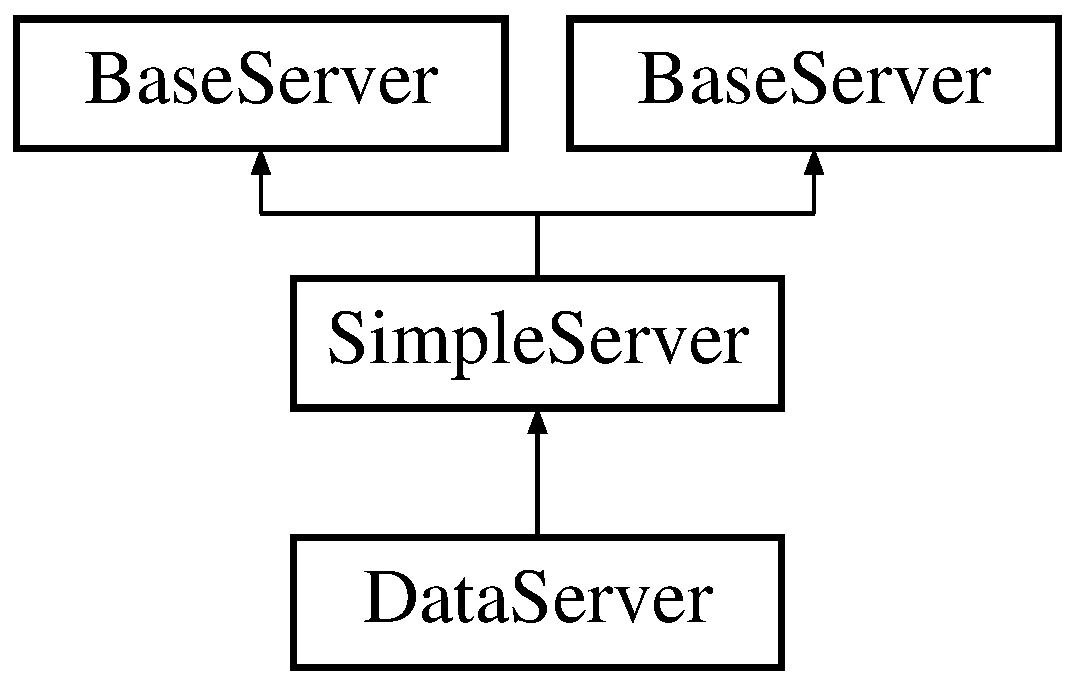
\includegraphics[height=3.000000cm]{classDataServer}
\end{center}
\end{figure}
\subsection*{Public Member Functions}
\begin{DoxyCompactItemize}
\item 
\hyperlink{classDataServer_acf71809c4ac2e7eb13d1ad0c6c139b15}{Data\-Server} ()
\item 
\hyperlink{classDataServer_ab4f08bb5349b6b9e021da97db65f1928}{$\sim$\-Data\-Server} ()
\item 
void \hyperlink{classDataServer_aca0d13b666d0a9d17f06b028a4a0f3f6}{set\-App\-Name} (const char $\ast$name)
\item 
int \hyperlink{classDataServer_a9e4b2229d17ab4d8653da5633f243a74}{get\-App\-Id} ()
\item 
void \hyperlink{classDataServer_ab701f76c95c4960824b7c9b587bdcae3}{read\-Inifile} (const char $\ast$\hyperlink{classDataServer_adb52183f12445a883b10c7081fa828a3}{inifile}, const char $\ast$module=0)
\item 
void \hyperlink{classDataServer_a89f7c5443aca4a3f7ed0860d00b0300c}{run\-As\-Daemon} (bool flag=true)
\item 
void \hyperlink{classDataServer_aa625ea002a9ab9b4cfdbb90807a1d67d}{get\-Next\-Sample} (int $\ast$i\-Sample, double $\ast$t\-Wait)
\item 
void \hyperlink{classDataServer_ab9b3333d6a5f872fd5f1e0d8010086a2}{get\-Next\-Sample} (int $\ast$i\-Sample, struct timeval $\ast$t\-Wait)
\item 
int \hyperlink{classDataServer_ac45cfcc0fca260f2283bd563281b4efa}{handle\-\_\-timeout} ()
\item 
int \hyperlink{classDataServer_a0b951c305048d917262e1017b6f7db24}{read\-\_\-from\-\_\-keyboard} ()
\item 
void \hyperlink{classDataServer_a726b0971e705894e243726640ecb7db0}{execute\-Cmd} (int client, short cmd, unsigned int $\ast$arg, short n)
\item 
void \hyperlink{classDataServer_a3977ab6cd0fde850d17c8b04885ad088}{run\-Readout} (F\-I\-L\-E $\ast$\hyperlink{classBaseServer_a9ad43261a042fbeeafee33ca4c0b3fd3}{fout})
\item 
void \hyperlink{classDataServer_a4de71f44e04b81e8d054462e94b087aa}{analyse\-Timing} (struct timeval $\ast$t)
\item 
void \hyperlink{classDataServer_afa17781b543e10b8ecc6f07ab77851f1}{display\-Status} (F\-I\-L\-E $\ast$\hyperlink{classBaseServer_a9ad43261a042fbeeafee33ca4c0b3fd3}{fout})
\item 
void \hyperlink{classDataServer_a0a5c1420e056418d02473db5ca5ec6ba}{simulate} ()
\item 
void \hyperlink{classDataServer_a6d3ab96ddbcf7bf5cff1565dc081b960}{sim\-Q\-D\-Data} (struct timeval t)
\item 
void \hyperlink{classDataServer_aa1e7d4724bbedec466f7c76f549b243b}{qd} (double $\ast$analog, int n)
\end{DoxyCompactItemize}
\subsection*{Public Attributes}
\begin{DoxyCompactItemize}
\item 
int \hyperlink{classDataServer_a85f6bfc815d5da78904704e04f58de4a}{sim\-Data\-Index}
\end{DoxyCompactItemize}
\subsection*{Private Attributes}
\begin{DoxyCompactItemize}
\item 
int \hyperlink{classDataServer_a2336dffa57e35c69c5ae0927d5e9e052}{app\-Id}
\item 
std\-::string \hyperlink{classDataServer_a8a26d65b11f0160c99cc00ab4a700a37}{app\-Name}
\item 
bool \hyperlink{classDataServer_a6dec7e960603680e4114abc5b91a8457}{run\-Daemon}
\item 
int \hyperlink{classDataServer_a0b926a7dc0e5ddcf958abedd937c362b}{t\-Sample\-From\-Inifile}
\item 
int \hyperlink{classDataServer_a099becd424d2c231270d8bf7682f86f7}{n\-Modules}
\item 
std\-::string \hyperlink{classDataServer_a38e8fd47db320927a4e7fe20226dc23d}{module\-Name}
\item 
std\-::string $\ast$ \hyperlink{classDataServer_ac2f86dedb120b60f6da583a3931f48a7}{module\-Type}
\item 
int $\ast$ \hyperlink{classDataServer_a4f01751e8d4a8d1ca9fd0e8cbb1240bb}{module\-Number}
\item 
std\-::string $\ast$ \hyperlink{classDataServer_a746d543bae3ea60b7c617413951c8e3c}{ini\-Group}
\item 
\hyperlink{classDAQDevice}{D\-A\-Q\-Device} $\ast$$\ast$ \hyperlink{classDataServer_a633e024ceb49f38f68a3f2cff5303cb4}{dev}
\item 
int \hyperlink{classDataServer_a6ef6ff1d012d3d199bd2d4ea2889e1fc}{n\-Groups}
\item 
unsigned long \hyperlink{classDataServer_a607273a35cc1cd03b19d548503ad7831}{samples\-N}
\item 
long long \hyperlink{classDataServer_abc58efaf6db25b7e8160a3adf62590af}{timing\-N}
\item 
long long \hyperlink{classDataServer_af821fc16f79698b3986813f7fce05cc1}{timing\-Sum}
\item 
long long \hyperlink{classDataServer_a4179f96aea793a3f9d4b4269c91af858}{timing\-Sum2}
\item 
long long \hyperlink{classDataServer_a271a282c615df76055fa1c2e83dbd3ab}{timing\-Min}
\item 
long long \hyperlink{classDataServer_ad02c5071511d4abd77be83a3bd74284f}{timing\-Max}
\item 
int \hyperlink{classDataServer_a63d42e1d7442a10dfcb4416b22e3cd94}{n\-Samples\-Skipped}
\item 
std\-::string \hyperlink{classDataServer_adb52183f12445a883b10c7081fa828a3}{inifile}
\item 
std\-::string \hyperlink{classDataServer_a7c825f2bc5af741b549dfd9b85d75bd3}{filename}
\item 
std\-::string \hyperlink{classDataServer_ae852f154e0a58505271bbcc9f2e23e28}{filename\-Tmpl}
\item 
std\-::string \hyperlink{classDataServer_a06a82d3d332afe39f6e56c9521abf5b1}{basedir}
\item 
std\-::string \hyperlink{classDataServer_afdc8023d653417275c503ceef21d5b35}{basedir\-Tmpl}
\item 
F\-I\-L\-E $\ast$ \hyperlink{classDataServer_a9b3b01c8057f00335cc4d81afb8d177a}{flog}
\item 
std\-::string \hyperlink{classDataServer_ad9f401ae56859aeb3518ca595a9849ad}{logfile}
\item 
std\-::string \hyperlink{classDataServer_adbd30fd13ec1fec779c48b942446f205}{qd\-Path}
\item 
std\-::string \hyperlink{classDataServer_a66169555f6156b14a11d88110660189d}{qd\-Config}
\item 
int \hyperlink{classDataServer_a69f0486314e244364a297310559446d7}{qd\-T\-Sample}
\item 
int \hyperlink{classDataServer_a61cfe7444488df95ed8a89bbb34823a1}{qd\-N\-Sensors}
\end{DoxyCompactItemize}
\subsection*{Additional Inherited Members}


\subsection{Detailed Description}
\begin{DoxyVerb}Recorder process for background data.
The background data is collected at the
telescopes and transfered to the central
data collection point (this class).

The background data is collected using a client server concept. At every
connected telescope a readout process is started that afterwards autonomuosly
sends the data to the server running at the eyePC writing the data to the file.

The background data is stored in text format. The data of every parameter
introduced by a header line containing certain parmeters necessary to
interprete the data. There is a master header for a complete set of background
data.

The following box shows a sample call of the background recorder.
\end{DoxyVerb}
 \begin{DoxyVerb}  TsBackgroundLoop *bgrec;
  Pbus *thePbus;

  Pbus::init(inifile.c_str());


  // Create recorder
  bgrec = new TsBackgroundLoop();
  bgrec->readInifile(inifile.c_str());

  bgrec->setLogfile(stdout);

  // Set parameter: Period length, selected parameter, file, ....
  bgrec->setParameter(name, tSample, 0, selRecord, selDisplay, runType.c_str());  // no output to file, take data every 5s

  // Run background recorder
  // The readout process is started at all connected telescopes
  bgrec->runReadout(stdout);

  delete bgrec;
\end{DoxyVerb}


\begin{DoxyRefDesc}{Todo}
\item[\hyperlink{todo__todo000013}{Todo}]Streamer methoden einfhren, es erscheint unsauber, die Methoden mit zu kopieren !!! 

Wie kann man eine verlorene Verbindung erkennen? Wie kann der Server-\/\-Verbindungen l�en?
\begin{DoxyItemize}
\item Bleiben immer so viele Verbindungen liegen? Tw. wird eine weiterer Aufruf hierdurch sogar blockiert?!
\item Zeitnahmedaten mit in die Daten aufnehmen!!! �erarbeiten der display-\/\-Funktionen.
\item Definition des Befehlssatzen in einer Struktur, die von beiden Seiten verwendet wird!
\item Verwenden von R\-O\-O\-T-\/\-Trees zum Abspeichern der Daten
\item Integration in Pbusdaemon / oder ein separates Programm, das vom Pbusdaemon aufgerufen wird?!
\item Display-\/\-Programm, das sich ebenfalls an den Server ankoppelt.
\end{DoxyItemize}\end{DoxyRefDesc}
\begin{DoxyVerb}- Test mit echter Hardware: Werden die Daten korrekt bertragen
- Test mit mehreren Teleskopen
- Test mit automatischem Start ber Pbusdaemon
- Erweiterung des TsBackground-Formates fr die neuen Variablen
- Dokumentation der Background-Loop (Konzept / Start / Konfiguration / ...)
- Speichern im Root-Format, Aufteilung in Branches
- Beispielhaftes Display-Modul (ncurses) entwerfen
- Histogramming-Modul / Stern-Monitor ankoppeln
\end{DoxyVerb}


\begin{DoxyRefDesc}{Todo}
\item[\hyperlink{todo__todo000014}{Todo}]The recorder does not work with a connection started via ssh tunnel. The readout process at the mirrorpc's seem to have problems to connect to the proper recorder server?!\end{DoxyRefDesc}


\subsection{Constructor \& Destructor Documentation}
\hypertarget{classDataServer_acf71809c4ac2e7eb13d1ad0c6c139b15}{\index{Data\-Server@{Data\-Server}!Data\-Server@{Data\-Server}}
\index{Data\-Server@{Data\-Server}!DataServer@{Data\-Server}}
\subsubsection[{Data\-Server}]{\setlength{\rightskip}{0pt plus 5cm}Data\-Server\-::\-Data\-Server (
\begin{DoxyParamCaption}
{}
\end{DoxyParamCaption}
)}}\label{classDataServer_acf71809c4ac2e7eb13d1ad0c6c139b15}
\hypertarget{classDataServer_ab4f08bb5349b6b9e021da97db65f1928}{\index{Data\-Server@{Data\-Server}!$\sim$\-Data\-Server@{$\sim$\-Data\-Server}}
\index{$\sim$\-Data\-Server@{$\sim$\-Data\-Server}!DataServer@{Data\-Server}}
\subsubsection[{$\sim$\-Data\-Server}]{\setlength{\rightskip}{0pt plus 5cm}Data\-Server\-::$\sim$\-Data\-Server (
\begin{DoxyParamCaption}
{}
\end{DoxyParamCaption}
)}}\label{classDataServer_ab4f08bb5349b6b9e021da97db65f1928}


\subsection{Member Function Documentation}
\hypertarget{classDataServer_a4de71f44e04b81e8d054462e94b087aa}{\index{Data\-Server@{Data\-Server}!analyse\-Timing@{analyse\-Timing}}
\index{analyse\-Timing@{analyse\-Timing}!DataServer@{Data\-Server}}
\subsubsection[{analyse\-Timing}]{\setlength{\rightskip}{0pt plus 5cm}void Data\-Server\-::analyse\-Timing (
\begin{DoxyParamCaption}
\item[{struct timeval $\ast$}]{t}
\end{DoxyParamCaption}
)}}\label{classDataServer_a4de71f44e04b81e8d054462e94b087aa}
Analyse timing \hypertarget{classDataServer_afa17781b543e10b8ecc6f07ab77851f1}{\index{Data\-Server@{Data\-Server}!display\-Status@{display\-Status}}
\index{display\-Status@{display\-Status}!DataServer@{Data\-Server}}
\subsubsection[{display\-Status}]{\setlength{\rightskip}{0pt plus 5cm}void Data\-Server\-::display\-Status (
\begin{DoxyParamCaption}
\item[{F\-I\-L\-E $\ast$}]{fout}
\end{DoxyParamCaption}
)}}\label{classDataServer_afa17781b543e10b8ecc6f07ab77851f1}
Display status of readout process \hypertarget{classDataServer_a726b0971e705894e243726640ecb7db0}{\index{Data\-Server@{Data\-Server}!execute\-Cmd@{execute\-Cmd}}
\index{execute\-Cmd@{execute\-Cmd}!DataServer@{Data\-Server}}
\subsubsection[{execute\-Cmd}]{\setlength{\rightskip}{0pt plus 5cm}void Data\-Server\-::execute\-Cmd (
\begin{DoxyParamCaption}
\item[{int}]{client, }
\item[{short}]{cmd, }
\item[{unsigned int $\ast$}]{arg, }
\item[{short}]{n}
\end{DoxyParamCaption}
)\hspace{0.3cm}{\ttfamily [virtual]}}}\label{classDataServer_a726b0971e705894e243726640ecb7db0}
Execute the command 

Reimplemented from \hyperlink{classSimpleServer_ad8244094d9e1806edaa166093c94bd24}{Simple\-Server}.

\hypertarget{classDataServer_a9e4b2229d17ab4d8653da5633f243a74}{\index{Data\-Server@{Data\-Server}!get\-App\-Id@{get\-App\-Id}}
\index{get\-App\-Id@{get\-App\-Id}!DataServer@{Data\-Server}}
\subsubsection[{get\-App\-Id}]{\setlength{\rightskip}{0pt plus 5cm}int Data\-Server\-::get\-App\-Id (
\begin{DoxyParamCaption}
{}
\end{DoxyParamCaption}
)}}\label{classDataServer_a9e4b2229d17ab4d8653da5633f243a74}
Get the number of the application \hypertarget{classDataServer_aa625ea002a9ab9b4cfdbb90807a1d67d}{\index{Data\-Server@{Data\-Server}!get\-Next\-Sample@{get\-Next\-Sample}}
\index{get\-Next\-Sample@{get\-Next\-Sample}!DataServer@{Data\-Server}}
\subsubsection[{get\-Next\-Sample}]{\setlength{\rightskip}{0pt plus 5cm}void Data\-Server\-::get\-Next\-Sample (
\begin{DoxyParamCaption}
\item[{int $\ast$}]{i\-Sample, }
\item[{double $\ast$}]{t\-Wait}
\end{DoxyParamCaption}
)}}\label{classDataServer_aa625ea002a9ab9b4cfdbb90807a1d67d}
Get time until next sample and it's id \hypertarget{classDataServer_ab9b3333d6a5f872fd5f1e0d8010086a2}{\index{Data\-Server@{Data\-Server}!get\-Next\-Sample@{get\-Next\-Sample}}
\index{get\-Next\-Sample@{get\-Next\-Sample}!DataServer@{Data\-Server}}
\subsubsection[{get\-Next\-Sample}]{\setlength{\rightskip}{0pt plus 5cm}void Data\-Server\-::get\-Next\-Sample (
\begin{DoxyParamCaption}
\item[{int $\ast$}]{i\-Sample, }
\item[{struct timeval $\ast$}]{t\-Wait}
\end{DoxyParamCaption}
)}}\label{classDataServer_ab9b3333d6a5f872fd5f1e0d8010086a2}
\hypertarget{classDataServer_ac45cfcc0fca260f2283bd563281b4efa}{\index{Data\-Server@{Data\-Server}!handle\-\_\-timeout@{handle\-\_\-timeout}}
\index{handle\-\_\-timeout@{handle\-\_\-timeout}!DataServer@{Data\-Server}}
\subsubsection[{handle\-\_\-timeout}]{\setlength{\rightskip}{0pt plus 5cm}int Data\-Server\-::handle\-\_\-timeout (
\begin{DoxyParamCaption}
{}
\end{DoxyParamCaption}
)\hspace{0.3cm}{\ttfamily [virtual]}}}\label{classDataServer_ac45cfcc0fca260f2283bd563281b4efa}
Handler for the timeout 

Reimplemented from \hyperlink{classBaseServer_a892cf59b889f59d73031108cfab07772}{Base\-Server}.

\hypertarget{classDataServer_aa1e7d4724bbedec466f7c76f549b243b}{\index{Data\-Server@{Data\-Server}!qd@{qd}}
\index{qd@{qd}!DataServer@{Data\-Server}}
\subsubsection[{qd}]{\setlength{\rightskip}{0pt plus 5cm}void Data\-Server\-::qd (
\begin{DoxyParamCaption}
\item[{double $\ast$}]{analog, }
\item[{int}]{n}
\end{DoxyParamCaption}
)}}\label{classDataServer_aa1e7d4724bbedec466f7c76f549b243b}
Generate analog data input

Simulate Q\-D signal matrix. Use P\-C time to calculate a sinus wave plus some noise. \hypertarget{classDataServer_a0b951c305048d917262e1017b6f7db24}{\index{Data\-Server@{Data\-Server}!read\-\_\-from\-\_\-keyboard@{read\-\_\-from\-\_\-keyboard}}
\index{read\-\_\-from\-\_\-keyboard@{read\-\_\-from\-\_\-keyboard}!DataServer@{Data\-Server}}
\subsubsection[{read\-\_\-from\-\_\-keyboard}]{\setlength{\rightskip}{0pt plus 5cm}int Data\-Server\-::read\-\_\-from\-\_\-keyboard (
\begin{DoxyParamCaption}
{}
\end{DoxyParamCaption}
)\hspace{0.3cm}{\ttfamily [virtual]}}}\label{classDataServer_a0b951c305048d917262e1017b6f7db24}
Keyboard interface for interactive control (only for compatibility reasons 

Reimplemented from \hyperlink{classBaseServer_a2c5a73b3bd9950a7809ac2a353061960}{Base\-Server}.

\hypertarget{classDataServer_ab701f76c95c4960824b7c9b587bdcae3}{\index{Data\-Server@{Data\-Server}!read\-Inifile@{read\-Inifile}}
\index{read\-Inifile@{read\-Inifile}!DataServer@{Data\-Server}}
\subsubsection[{read\-Inifile}]{\setlength{\rightskip}{0pt plus 5cm}void Data\-Server\-::read\-Inifile (
\begin{DoxyParamCaption}
\item[{const char $\ast$}]{inifile, }
\item[{const char $\ast$}]{module = {\ttfamily 0}}
\end{DoxyParamCaption}
)}}\label{classDataServer_ab701f76c95c4960824b7c9b587bdcae3}
Read parameter from inifile \hypertarget{classDataServer_a89f7c5443aca4a3f7ed0860d00b0300c}{\index{Data\-Server@{Data\-Server}!run\-As\-Daemon@{run\-As\-Daemon}}
\index{run\-As\-Daemon@{run\-As\-Daemon}!DataServer@{Data\-Server}}
\subsubsection[{run\-As\-Daemon}]{\setlength{\rightskip}{0pt plus 5cm}void Data\-Server\-::run\-As\-Daemon (
\begin{DoxyParamCaption}
\item[{bool}]{flag = {\ttfamily true}}
\end{DoxyParamCaption}
)}}\label{classDataServer_a89f7c5443aca4a3f7ed0860d00b0300c}
Set operation without interactive inputs \hypertarget{classDataServer_a3977ab6cd0fde850d17c8b04885ad088}{\index{Data\-Server@{Data\-Server}!run\-Readout@{run\-Readout}}
\index{run\-Readout@{run\-Readout}!DataServer@{Data\-Server}}
\subsubsection[{run\-Readout}]{\setlength{\rightskip}{0pt plus 5cm}void Data\-Server\-::run\-Readout (
\begin{DoxyParamCaption}
\item[{F\-I\-L\-E $\ast$}]{fout}
\end{DoxyParamCaption}
)}}\label{classDataServer_a3977ab6cd0fde850d17c8b04885ad088}
Start the server and all the client recording the telescopes background data. \hypertarget{classDataServer_aca0d13b666d0a9d17f06b028a4a0f3f6}{\index{Data\-Server@{Data\-Server}!set\-App\-Name@{set\-App\-Name}}
\index{set\-App\-Name@{set\-App\-Name}!DataServer@{Data\-Server}}
\subsubsection[{set\-App\-Name}]{\setlength{\rightskip}{0pt plus 5cm}void Data\-Server\-::set\-App\-Name (
\begin{DoxyParamCaption}
\item[{const char $\ast$}]{name}
\end{DoxyParamCaption}
)}}\label{classDataServer_aca0d13b666d0a9d17f06b028a4a0f3f6}
Change the default name of the application used to figure out the right inifile section \hypertarget{classDataServer_a6d3ab96ddbcf7bf5cff1565dc081b960}{\index{Data\-Server@{Data\-Server}!sim\-Q\-D\-Data@{sim\-Q\-D\-Data}}
\index{sim\-Q\-D\-Data@{sim\-Q\-D\-Data}!DataServer@{Data\-Server}}
\subsubsection[{sim\-Q\-D\-Data}]{\setlength{\rightskip}{0pt plus 5cm}void Data\-Server\-::sim\-Q\-D\-Data (
\begin{DoxyParamCaption}
\item[{struct timeval}]{t}
\end{DoxyParamCaption}
)}}\label{classDataServer_a6d3ab96ddbcf7bf5cff1565dc081b960}
Simulate data of the quench detection unit \hypertarget{classDataServer_a0a5c1420e056418d02473db5ca5ec6ba}{\index{Data\-Server@{Data\-Server}!simulate@{simulate}}
\index{simulate@{simulate}!DataServer@{Data\-Server}}
\subsubsection[{simulate}]{\setlength{\rightskip}{0pt plus 5cm}void Data\-Server\-::simulate (
\begin{DoxyParamCaption}
{}
\end{DoxyParamCaption}
)}}\label{classDataServer_a0a5c1420e056418d02473db5ca5ec6ba}


\subsection{Member Data Documentation}
\hypertarget{classDataServer_a2336dffa57e35c69c5ae0927d5e9e052}{\index{Data\-Server@{Data\-Server}!app\-Id@{app\-Id}}
\index{app\-Id@{app\-Id}!DataServer@{Data\-Server}}
\subsubsection[{app\-Id}]{\setlength{\rightskip}{0pt plus 5cm}int Data\-Server\-::app\-Id\hspace{0.3cm}{\ttfamily [private]}}}\label{classDataServer_a2336dffa57e35c69c5ae0927d5e9e052}
Every reader application has it's own I\-D \hypertarget{classDataServer_a8a26d65b11f0160c99cc00ab4a700a37}{\index{Data\-Server@{Data\-Server}!app\-Name@{app\-Name}}
\index{app\-Name@{app\-Name}!DataServer@{Data\-Server}}
\subsubsection[{app\-Name}]{\setlength{\rightskip}{0pt plus 5cm}std\-::string Data\-Server\-::app\-Name\hspace{0.3cm}{\ttfamily [private]}}}\label{classDataServer_a8a26d65b11f0160c99cc00ab4a700a37}
Name of the application. Used to select the application ini group. Default\-: \hyperlink{classReader}{Reader} \hypertarget{classDataServer_a06a82d3d332afe39f6e56c9521abf5b1}{\index{Data\-Server@{Data\-Server}!basedir@{basedir}}
\index{basedir@{basedir}!DataServer@{Data\-Server}}
\subsubsection[{basedir}]{\setlength{\rightskip}{0pt plus 5cm}std\-::string Data\-Server\-::basedir\hspace{0.3cm}{\ttfamily [private]}}}\label{classDataServer_a06a82d3d332afe39f6e56c9521abf5b1}
Basedir of the auger file \hypertarget{classDataServer_afdc8023d653417275c503ceef21d5b35}{\index{Data\-Server@{Data\-Server}!basedir\-Tmpl@{basedir\-Tmpl}}
\index{basedir\-Tmpl@{basedir\-Tmpl}!DataServer@{Data\-Server}}
\subsubsection[{basedir\-Tmpl}]{\setlength{\rightskip}{0pt plus 5cm}std\-::string Data\-Server\-::basedir\-Tmpl\hspace{0.3cm}{\ttfamily [private]}}}\label{classDataServer_afdc8023d653417275c503ceef21d5b35}
Template for the basedir of the auger file \hypertarget{classDataServer_a633e024ceb49f38f68a3f2cff5303cb4}{\index{Data\-Server@{Data\-Server}!dev@{dev}}
\index{dev@{dev}!DataServer@{Data\-Server}}
\subsubsection[{dev}]{\setlength{\rightskip}{0pt plus 5cm}{\bf D\-A\-Q\-Device}$\ast$$\ast$ Data\-Server\-::dev\hspace{0.3cm}{\ttfamily [private]}}}\label{classDataServer_a633e024ceb49f38f68a3f2cff5303cb4}
\hypertarget{classDataServer_a7c825f2bc5af741b549dfd9b85d75bd3}{\index{Data\-Server@{Data\-Server}!filename@{filename}}
\index{filename@{filename}!DataServer@{Data\-Server}}
\subsubsection[{filename}]{\setlength{\rightskip}{0pt plus 5cm}std\-::string Data\-Server\-::filename\hspace{0.3cm}{\ttfamily [private]}}}\label{classDataServer_a7c825f2bc5af741b549dfd9b85d75bd3}
Record filename \hypertarget{classDataServer_ae852f154e0a58505271bbcc9f2e23e28}{\index{Data\-Server@{Data\-Server}!filename\-Tmpl@{filename\-Tmpl}}
\index{filename\-Tmpl@{filename\-Tmpl}!DataServer@{Data\-Server}}
\subsubsection[{filename\-Tmpl}]{\setlength{\rightskip}{0pt plus 5cm}std\-::string Data\-Server\-::filename\-Tmpl\hspace{0.3cm}{\ttfamily [private]}}}\label{classDataServer_ae852f154e0a58505271bbcc9f2e23e28}
Template for the record filename \hypertarget{classDataServer_a9b3b01c8057f00335cc4d81afb8d177a}{\index{Data\-Server@{Data\-Server}!flog@{flog}}
\index{flog@{flog}!DataServer@{Data\-Server}}
\subsubsection[{flog}]{\setlength{\rightskip}{0pt plus 5cm}F\-I\-L\-E$\ast$ Data\-Server\-::flog\hspace{0.3cm}{\ttfamily [private]}}}\label{classDataServer_a9b3b01c8057f00335cc4d81afb8d177a}
F\-Ealarm log file name \hypertarget{classDataServer_adb52183f12445a883b10c7081fa828a3}{\index{Data\-Server@{Data\-Server}!inifile@{inifile}}
\index{inifile@{inifile}!DataServer@{Data\-Server}}
\subsubsection[{inifile}]{\setlength{\rightskip}{0pt plus 5cm}std\-::string Data\-Server\-::inifile\hspace{0.3cm}{\ttfamily [private]}}}\label{classDataServer_adb52183f12445a883b10c7081fa828a3}
\hypertarget{classDataServer_a746d543bae3ea60b7c617413951c8e3c}{\index{Data\-Server@{Data\-Server}!ini\-Group@{ini\-Group}}
\index{ini\-Group@{ini\-Group}!DataServer@{Data\-Server}}
\subsubsection[{ini\-Group}]{\setlength{\rightskip}{0pt plus 5cm}std\-::string$\ast$ Data\-Server\-::ini\-Group\hspace{0.3cm}{\ttfamily [private]}}}\label{classDataServer_a746d543bae3ea60b7c617413951c8e3c}
a group in the $\ast$.ini file \hypertarget{classDataServer_ad9f401ae56859aeb3518ca595a9849ad}{\index{Data\-Server@{Data\-Server}!logfile@{logfile}}
\index{logfile@{logfile}!DataServer@{Data\-Server}}
\subsubsection[{logfile}]{\setlength{\rightskip}{0pt plus 5cm}std\-::string Data\-Server\-::logfile\hspace{0.3cm}{\ttfamily [private]}}}\label{classDataServer_ad9f401ae56859aeb3518ca595a9849ad}
Name of the logfile \hypertarget{classDataServer_a38e8fd47db320927a4e7fe20226dc23d}{\index{Data\-Server@{Data\-Server}!module\-Name@{module\-Name}}
\index{module\-Name@{module\-Name}!DataServer@{Data\-Server}}
\subsubsection[{module\-Name}]{\setlength{\rightskip}{0pt plus 5cm}std\-::string Data\-Server\-::module\-Name\hspace{0.3cm}{\ttfamily [private]}}}\label{classDataServer_a38e8fd47db320927a4e7fe20226dc23d}
Module name as given in sensor list \hypertarget{classDataServer_a4f01751e8d4a8d1ca9fd0e8cbb1240bb}{\index{Data\-Server@{Data\-Server}!module\-Number@{module\-Number}}
\index{module\-Number@{module\-Number}!DataServer@{Data\-Server}}
\subsubsection[{module\-Number}]{\setlength{\rightskip}{0pt plus 5cm}int$\ast$ Data\-Server\-::module\-Number\hspace{0.3cm}{\ttfamily [private]}}}\label{classDataServer_a4f01751e8d4a8d1ca9fd0e8cbb1240bb}
Module number \hypertarget{classDataServer_ac2f86dedb120b60f6da583a3931f48a7}{\index{Data\-Server@{Data\-Server}!module\-Type@{module\-Type}}
\index{module\-Type@{module\-Type}!DataServer@{Data\-Server}}
\subsubsection[{module\-Type}]{\setlength{\rightskip}{0pt plus 5cm}std\-::string$\ast$ Data\-Server\-::module\-Type\hspace{0.3cm}{\ttfamily [private]}}}\label{classDataServer_ac2f86dedb120b60f6da583a3931f48a7}
module type describes the implementation, the class \hypertarget{classDataServer_a6ef6ff1d012d3d199bd2d4ea2889e1fc}{\index{Data\-Server@{Data\-Server}!n\-Groups@{n\-Groups}}
\index{n\-Groups@{n\-Groups}!DataServer@{Data\-Server}}
\subsubsection[{n\-Groups}]{\setlength{\rightskip}{0pt plus 5cm}int Data\-Server\-::n\-Groups\hspace{0.3cm}{\ttfamily [private]}}}\label{classDataServer_a6ef6ff1d012d3d199bd2d4ea2889e1fc}
Number of sensor groups \hypertarget{classDataServer_a099becd424d2c231270d8bf7682f86f7}{\index{Data\-Server@{Data\-Server}!n\-Modules@{n\-Modules}}
\index{n\-Modules@{n\-Modules}!DataServer@{Data\-Server}}
\subsubsection[{n\-Modules}]{\setlength{\rightskip}{0pt plus 5cm}int Data\-Server\-::n\-Modules\hspace{0.3cm}{\ttfamily [private]}}}\label{classDataServer_a099becd424d2c231270d8bf7682f86f7}
Number of D\-A\-Q modules added to the data server. The number is given by the entries in the inifile \hypertarget{classDataServer_a63d42e1d7442a10dfcb4416b22e3cd94}{\index{Data\-Server@{Data\-Server}!n\-Samples\-Skipped@{n\-Samples\-Skipped}}
\index{n\-Samples\-Skipped@{n\-Samples\-Skipped}!DataServer@{Data\-Server}}
\subsubsection[{n\-Samples\-Skipped}]{\setlength{\rightskip}{0pt plus 5cm}int Data\-Server\-::n\-Samples\-Skipped\hspace{0.3cm}{\ttfamily [private]}}}\label{classDataServer_a63d42e1d7442a10dfcb4416b22e3cd94}
Number of last samples skipped, because there was no vaild data / timestamp \hypertarget{classDataServer_a66169555f6156b14a11d88110660189d}{\index{Data\-Server@{Data\-Server}!qd\-Config@{qd\-Config}}
\index{qd\-Config@{qd\-Config}!DataServer@{Data\-Server}}
\subsubsection[{qd\-Config}]{\setlength{\rightskip}{0pt plus 5cm}std\-::string Data\-Server\-::qd\-Config\hspace{0.3cm}{\ttfamily [private]}}}\label{classDataServer_a66169555f6156b14a11d88110660189d}
Name of configuration file \hypertarget{classDataServer_a61cfe7444488df95ed8a89bbb34823a1}{\index{Data\-Server@{Data\-Server}!qd\-N\-Sensors@{qd\-N\-Sensors}}
\index{qd\-N\-Sensors@{qd\-N\-Sensors}!DataServer@{Data\-Server}}
\subsubsection[{qd\-N\-Sensors}]{\setlength{\rightskip}{0pt plus 5cm}int Data\-Server\-::qd\-N\-Sensors\hspace{0.3cm}{\ttfamily [private]}}}\label{classDataServer_a61cfe7444488df95ed8a89bbb34823a1}
Number of values (max 24) \hypertarget{classDataServer_adbd30fd13ec1fec779c48b942446f205}{\index{Data\-Server@{Data\-Server}!qd\-Path@{qd\-Path}}
\index{qd\-Path@{qd\-Path}!DataServer@{Data\-Server}}
\subsubsection[{qd\-Path}]{\setlength{\rightskip}{0pt plus 5cm}std\-::string Data\-Server\-::qd\-Path\hspace{0.3cm}{\ttfamily [private]}}}\label{classDataServer_adbd30fd13ec1fec779c48b942446f205}
Path to the Q\-D data \hypertarget{classDataServer_a69f0486314e244364a297310559446d7}{\index{Data\-Server@{Data\-Server}!qd\-T\-Sample@{qd\-T\-Sample}}
\index{qd\-T\-Sample@{qd\-T\-Sample}!DataServer@{Data\-Server}}
\subsubsection[{qd\-T\-Sample}]{\setlength{\rightskip}{0pt plus 5cm}int Data\-Server\-::qd\-T\-Sample\hspace{0.3cm}{\ttfamily [private]}}}\label{classDataServer_a69f0486314e244364a297310559446d7}
Sampling time (ms) \hypertarget{classDataServer_a6dec7e960603680e4114abc5b91a8457}{\index{Data\-Server@{Data\-Server}!run\-Daemon@{run\-Daemon}}
\index{run\-Daemon@{run\-Daemon}!DataServer@{Data\-Server}}
\subsubsection[{run\-Daemon}]{\setlength{\rightskip}{0pt plus 5cm}bool Data\-Server\-::run\-Daemon\hspace{0.3cm}{\ttfamily [private]}}}\label{classDataServer_a6dec7e960603680e4114abc5b91a8457}
Flag to start the server as daemon -\/ without interactive input \hypertarget{classDataServer_a607273a35cc1cd03b19d548503ad7831}{\index{Data\-Server@{Data\-Server}!samples\-N@{samples\-N}}
\index{samples\-N@{samples\-N}!DataServer@{Data\-Server}}
\subsubsection[{samples\-N}]{\setlength{\rightskip}{0pt plus 5cm}unsigned long Data\-Server\-::samples\-N\hspace{0.3cm}{\ttfamily [private]}}}\label{classDataServer_a607273a35cc1cd03b19d548503ad7831}
Number of samples (of timeout loop) \hypertarget{classDataServer_a85f6bfc815d5da78904704e04f58de4a}{\index{Data\-Server@{Data\-Server}!sim\-Data\-Index@{sim\-Data\-Index}}
\index{sim\-Data\-Index@{sim\-Data\-Index}!DataServer@{Data\-Server}}
\subsubsection[{sim\-Data\-Index}]{\setlength{\rightskip}{0pt plus 5cm}int Data\-Server\-::sim\-Data\-Index}}\label{classDataServer_a85f6bfc815d5da78904704e04f58de4a}
Write one long data file Index of the data files \hypertarget{classDataServer_ad02c5071511d4abd77be83a3bd74284f}{\index{Data\-Server@{Data\-Server}!timing\-Max@{timing\-Max}}
\index{timing\-Max@{timing\-Max}!DataServer@{Data\-Server}}
\subsubsection[{timing\-Max}]{\setlength{\rightskip}{0pt plus 5cm}long long Data\-Server\-::timing\-Max\hspace{0.3cm}{\ttfamily [private]}}}\label{classDataServer_ad02c5071511d4abd77be83a3bd74284f}
Maximal deviation \hypertarget{classDataServer_a271a282c615df76055fa1c2e83dbd3ab}{\index{Data\-Server@{Data\-Server}!timing\-Min@{timing\-Min}}
\index{timing\-Min@{timing\-Min}!DataServer@{Data\-Server}}
\subsubsection[{timing\-Min}]{\setlength{\rightskip}{0pt plus 5cm}long long Data\-Server\-::timing\-Min\hspace{0.3cm}{\ttfamily [private]}}}\label{classDataServer_a271a282c615df76055fa1c2e83dbd3ab}
Minimal deviation \hypertarget{classDataServer_abc58efaf6db25b7e8160a3adf62590af}{\index{Data\-Server@{Data\-Server}!timing\-N@{timing\-N}}
\index{timing\-N@{timing\-N}!DataServer@{Data\-Server}}
\subsubsection[{timing\-N}]{\setlength{\rightskip}{0pt plus 5cm}long long Data\-Server\-::timing\-N\hspace{0.3cm}{\ttfamily [private]}}}\label{classDataServer_abc58efaf6db25b7e8160a3adf62590af}
Number of analysed samples \hypertarget{classDataServer_af821fc16f79698b3986813f7fce05cc1}{\index{Data\-Server@{Data\-Server}!timing\-Sum@{timing\-Sum}}
\index{timing\-Sum@{timing\-Sum}!DataServer@{Data\-Server}}
\subsubsection[{timing\-Sum}]{\setlength{\rightskip}{0pt plus 5cm}long long Data\-Server\-::timing\-Sum\hspace{0.3cm}{\ttfamily [private]}}}\label{classDataServer_af821fc16f79698b3986813f7fce05cc1}
Sum of all deviations from the planned sample time \hypertarget{classDataServer_a4179f96aea793a3f9d4b4269c91af858}{\index{Data\-Server@{Data\-Server}!timing\-Sum2@{timing\-Sum2}}
\index{timing\-Sum2@{timing\-Sum2}!DataServer@{Data\-Server}}
\subsubsection[{timing\-Sum2}]{\setlength{\rightskip}{0pt plus 5cm}long long Data\-Server\-::timing\-Sum2\hspace{0.3cm}{\ttfamily [private]}}}\label{classDataServer_a4179f96aea793a3f9d4b4269c91af858}
Sum of squares from the the planned sample time \hypertarget{classDataServer_a0b926a7dc0e5ddcf958abedd937c362b}{\index{Data\-Server@{Data\-Server}!t\-Sample\-From\-Inifile@{t\-Sample\-From\-Inifile}}
\index{t\-Sample\-From\-Inifile@{t\-Sample\-From\-Inifile}!DataServer@{Data\-Server}}
\subsubsection[{t\-Sample\-From\-Inifile}]{\setlength{\rightskip}{0pt plus 5cm}int Data\-Server\-::t\-Sample\-From\-Inifile\hspace{0.3cm}{\ttfamily [private]}}}\label{classDataServer_a0b926a7dc0e5ddcf958abedd937c362b}
Sampling time (ms) 

The documentation for this class was generated from the following files\-:\begin{DoxyCompactItemize}
\item 
/home/ntj/\-Development/phd/kitcube-\/tools/src/kitcube-\/data/\hyperlink{dataserver_8h}{dataserver.\-h}\item 
/home/ntj/\-Development/phd/kitcube-\/tools/src/kitcube-\/data/\hyperlink{dataserver_8cpp}{dataserver.\-cpp}\end{DoxyCompactItemize}

\hypertarget{classdreim}{\section{dreim Class Reference}
\label{classdreim}\index{dreim@{dreim}}
}


{\ttfamily \#include $<$3m.\-h$>$}

Inheritance diagram for dreim\-:\begin{figure}[H]
\begin{center}
\leavevmode
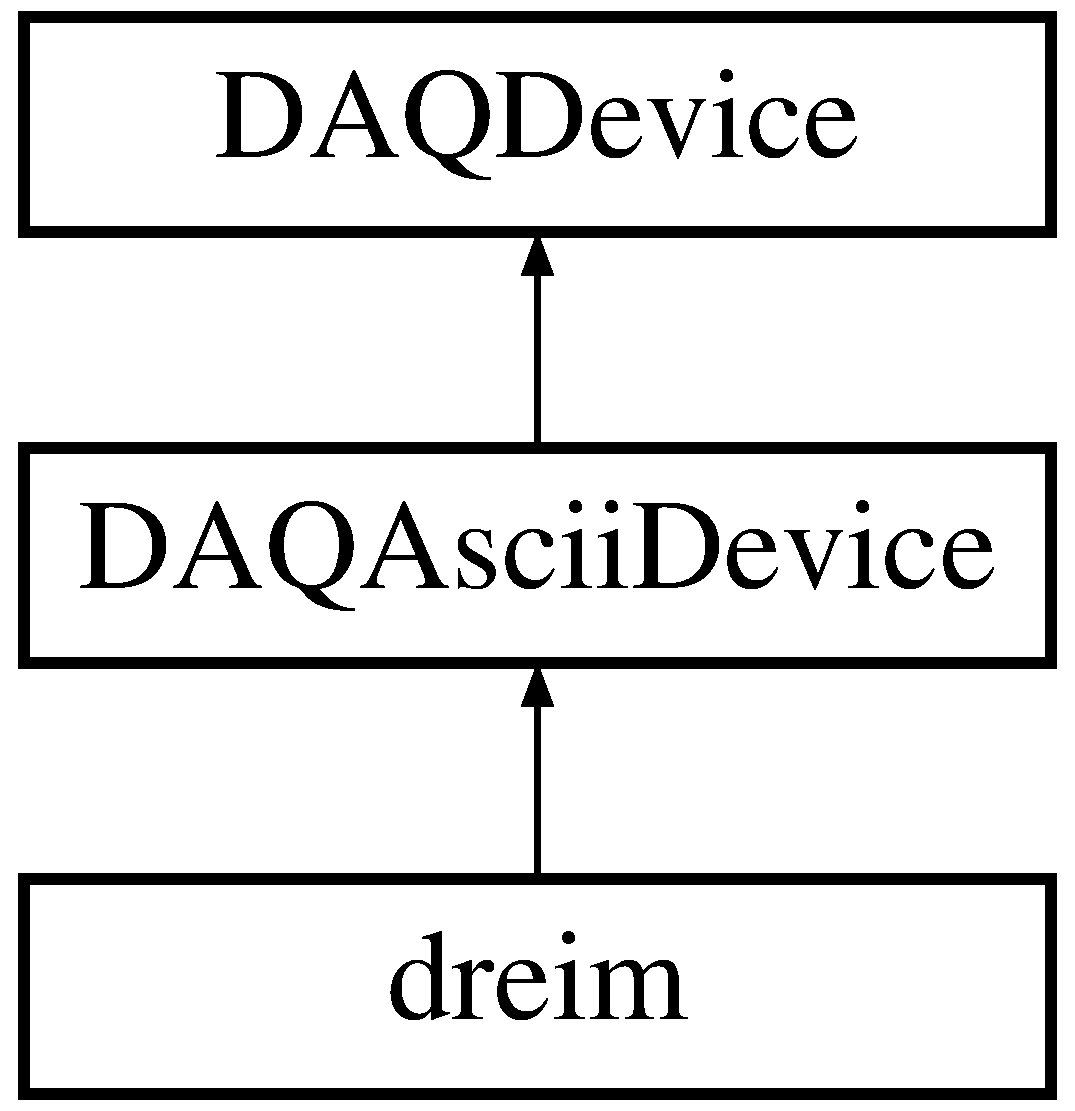
\includegraphics[height=3.000000cm]{classdreim}
\end{center}
\end{figure}
\subsection*{Public Member Functions}
\begin{DoxyCompactItemize}
\item 
\hyperlink{classdreim_ad5b00af326cf07b655691ee8644b9a44}{dreim} ()
\item 
\hyperlink{classdreim_a6f2a2a0a6694900935ba67cb198cc914}{$\sim$dreim} ()
\item 
void \hyperlink{classdreim_ae519ec4beeebe38402cdae1d475f1aaa}{set\-Config\-Defaults} ()
\item 
int \hyperlink{classdreim_a298f4f39711f41fd5e69d562d2e74bb7}{read\-Header} (const char $\ast$\hyperlink{classDAQDevice_a7f9cda7cf5b41f6b134c313477e9644b}{filename})
\item 
int \hyperlink{classdreim_ab0adce023f0af72491fe36dc2e228a4f}{parse\-Data} (char $\ast$line, struct timeval $\ast$l\-\_\-t\-Data, double $\ast$\hyperlink{classDAQDevice_ad148188c57598fdf4fd4c1c333aeb0d8}{sensor\-Value})
\item 
unsigned int \hyperlink{classdreim_a32184278a7ac6d365217f3e6b1023067}{get\-Sensor\-Group} ()
\end{DoxyCompactItemize}
\subsection*{Private Member Functions}
\begin{DoxyCompactItemize}
\item 
double \hyperlink{classdreim_a087d1cf984ffc5da8b6829cff898a6d0}{convert\-\_\-coordinate} (char $\ast$coordinate\-\_\-string)
\end{DoxyCompactItemize}
\subsection*{Additional Inherited Members}


\subsection{Constructor \& Destructor Documentation}
\hypertarget{classdreim_ad5b00af326cf07b655691ee8644b9a44}{\index{dreim@{dreim}!dreim@{dreim}}
\index{dreim@{dreim}!dreim@{dreim}}
\subsubsection[{dreim}]{\setlength{\rightskip}{0pt plus 5cm}dreim\-::dreim (
\begin{DoxyParamCaption}
{}
\end{DoxyParamCaption}
)}}\label{classdreim_ad5b00af326cf07b655691ee8644b9a44}
\hypertarget{classdreim_a6f2a2a0a6694900935ba67cb198cc914}{\index{dreim@{dreim}!$\sim$dreim@{$\sim$dreim}}
\index{$\sim$dreim@{$\sim$dreim}!dreim@{dreim}}
\subsubsection[{$\sim$dreim}]{\setlength{\rightskip}{0pt plus 5cm}dreim\-::$\sim$dreim (
\begin{DoxyParamCaption}
{}
\end{DoxyParamCaption}
)}}\label{classdreim_a6f2a2a0a6694900935ba67cb198cc914}


\subsection{Member Function Documentation}
\hypertarget{classdreim_a087d1cf984ffc5da8b6829cff898a6d0}{\index{dreim@{dreim}!convert\-\_\-coordinate@{convert\-\_\-coordinate}}
\index{convert\-\_\-coordinate@{convert\-\_\-coordinate}!dreim@{dreim}}
\subsubsection[{convert\-\_\-coordinate}]{\setlength{\rightskip}{0pt plus 5cm}double dreim\-::convert\-\_\-coordinate (
\begin{DoxyParamCaption}
\item[{char $\ast$}]{coordinate\-\_\-string}
\end{DoxyParamCaption}
)\hspace{0.3cm}{\ttfamily [private]}}}\label{classdreim_a087d1cf984ffc5da8b6829cff898a6d0}
\hypertarget{classdreim_a32184278a7ac6d365217f3e6b1023067}{\index{dreim@{dreim}!get\-Sensor\-Group@{get\-Sensor\-Group}}
\index{get\-Sensor\-Group@{get\-Sensor\-Group}!dreim@{dreim}}
\subsubsection[{get\-Sensor\-Group}]{\setlength{\rightskip}{0pt plus 5cm}unsigned int dreim\-::get\-Sensor\-Group (
\begin{DoxyParamCaption}
{}
\end{DoxyParamCaption}
)\hspace{0.3cm}{\ttfamily [virtual]}}}\label{classdreim_a32184278a7ac6d365217f3e6b1023067}
Define a sensor group number for all the availble sensor group files 

Reimplemented from \hyperlink{classDAQDevice_a61d08492a11c30944dfaf3b86115abe8}{D\-A\-Q\-Device}.

\hypertarget{classdreim_ab0adce023f0af72491fe36dc2e228a4f}{\index{dreim@{dreim}!parse\-Data@{parse\-Data}}
\index{parse\-Data@{parse\-Data}!dreim@{dreim}}
\subsubsection[{parse\-Data}]{\setlength{\rightskip}{0pt plus 5cm}int dreim\-::parse\-Data (
\begin{DoxyParamCaption}
\item[{char $\ast$}]{line, }
\item[{struct timeval $\ast$}]{l\-\_\-t\-Data, }
\item[{double $\ast$}]{sensor\-Value}
\end{DoxyParamCaption}
)\hspace{0.3cm}{\ttfamily [virtual]}}}\label{classdreim_ab0adce023f0af72491fe36dc2e228a4f}
Read the data from the current line of the data file. \begin{DoxyReturn}{Returns}
-\/1 no data found, skip storage 0 sucess, store data, 1 read another line 
\end{DoxyReturn}


Reimplemented from \hyperlink{classDAQAsciiDevice_a9c20d9d69af4ba1641dbc82dd5be2aa5}{D\-A\-Q\-Ascii\-Device}.

\hypertarget{classdreim_a298f4f39711f41fd5e69d562d2e74bb7}{\index{dreim@{dreim}!read\-Header@{read\-Header}}
\index{read\-Header@{read\-Header}!dreim@{dreim}}
\subsubsection[{read\-Header}]{\setlength{\rightskip}{0pt plus 5cm}int dreim\-::read\-Header (
\begin{DoxyParamCaption}
\item[{const char $\ast$}]{header}
\end{DoxyParamCaption}
)\hspace{0.3cm}{\ttfamily [virtual]}}}\label{classdreim_a298f4f39711f41fd5e69d562d2e74bb7}
Get time until next sample and it's id 

Reimplemented from \hyperlink{classDAQAsciiDevice_a5fce725c52b70ef2f56a34b32a03e15d}{D\-A\-Q\-Ascii\-Device}.

\hypertarget{classdreim_ae519ec4beeebe38402cdae1d475f1aaa}{\index{dreim@{dreim}!set\-Config\-Defaults@{set\-Config\-Defaults}}
\index{set\-Config\-Defaults@{set\-Config\-Defaults}!dreim@{dreim}}
\subsubsection[{set\-Config\-Defaults}]{\setlength{\rightskip}{0pt plus 5cm}void dreim\-::set\-Config\-Defaults (
\begin{DoxyParamCaption}
{}
\end{DoxyParamCaption}
)\hspace{0.3cm}{\ttfamily [virtual]}}}\label{classdreim_ae519ec4beeebe38402cdae1d475f1aaa}
The function is called before reading the configuration from the inifile. Use this fucntion in the module specific implementation to override the standard defaults 

Reimplemented from \hyperlink{classDAQDevice_a7685cec80865752cc0ef3ab49c6c2277}{D\-A\-Q\-Device}.



The documentation for this class was generated from the following files\-:\begin{DoxyCompactItemize}
\item 
/home/ntj/\-Development/phd/kitcube-\/tools/src/kitcube-\/devices/\hyperlink{3m_8h}{3m.\-h}\item 
/home/ntj/\-Development/phd/kitcube-\/tools/src/kitcube-\/devices/\hyperlink{3m_8cpp}{3m.\-cpp}\end{DoxyCompactItemize}

\hypertarget{classgps}{\section{gps Class Reference}
\label{classgps}\index{gps@{gps}}
}


{\ttfamily \#include $<$gps.\-h$>$}

Inheritance diagram for gps\-:\begin{figure}[H]
\begin{center}
\leavevmode
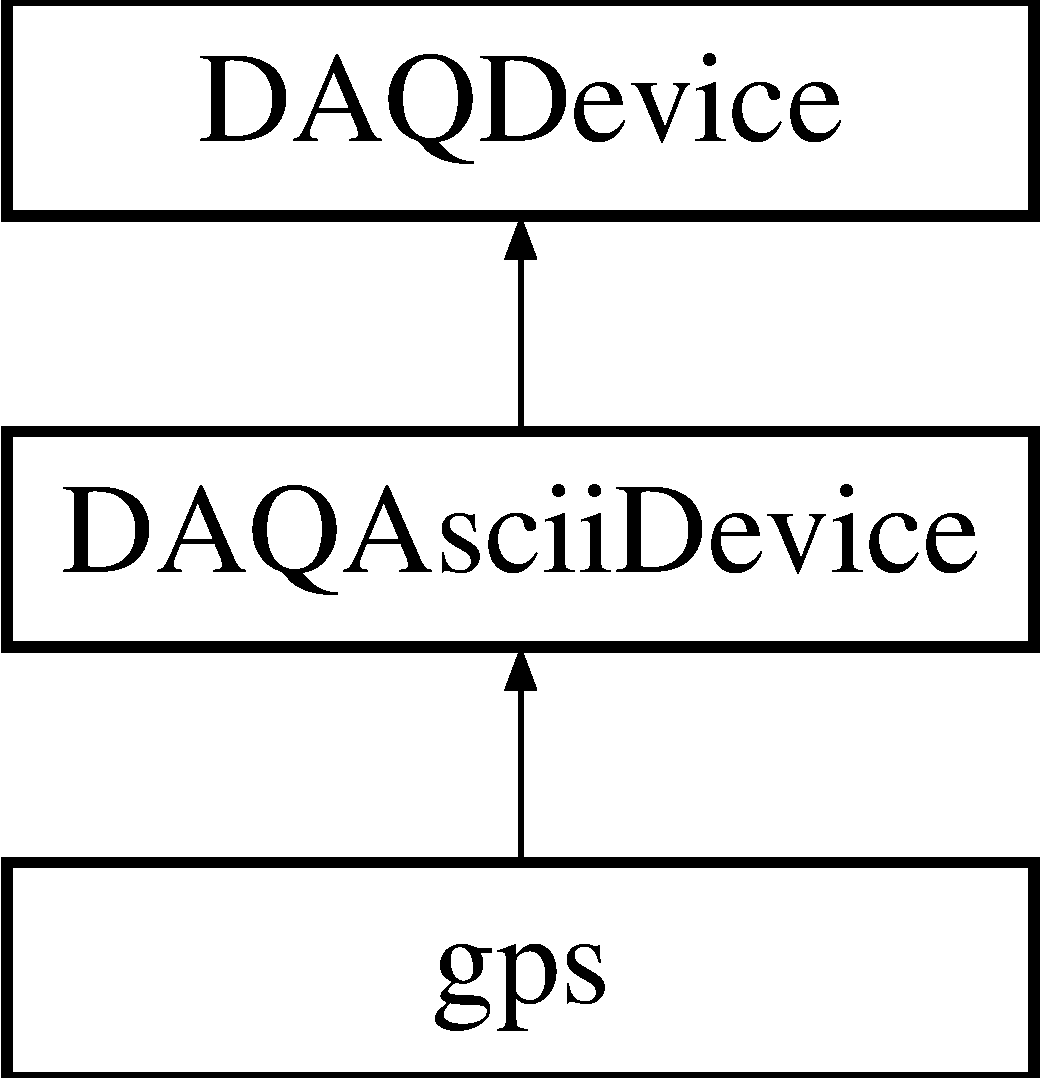
\includegraphics[height=3.000000cm]{classgps}
\end{center}
\end{figure}
\subsection*{Public Member Functions}
\begin{DoxyCompactItemize}
\item 
\hyperlink{classgps_a13b491233eeef0a9934e8d86db776949}{gps} ()
\item 
\hyperlink{classgps_a2a5bb1cd2bb43b8d2a1cacc7ab34f46e}{$\sim$gps} ()
\item 
void \hyperlink{classgps_a55f655de8f378da212ec92fd3283bb83}{set\-Config\-Defaults} ()
\item 
int \hyperlink{classgps_a37400cebc4929e7b30305c1b361f6309}{read\-Header} (const char $\ast$\hyperlink{classDAQDevice_a7f9cda7cf5b41f6b134c313477e9644b}{filename})
\item 
int \hyperlink{classgps_a8dc22ee8632e62c0547a782708b0238a}{parse\-Data} (char $\ast$line, struct timeval $\ast$l\-\_\-t\-Data, double $\ast$\hyperlink{classDAQDevice_ad148188c57598fdf4fd4c1c333aeb0d8}{sensor\-Value})
\item 
unsigned int \hyperlink{classgps_a3735ebac4b699c531c8ec24015bc9c89}{get\-Sensor\-Group} ()
\end{DoxyCompactItemize}
\subsection*{Additional Inherited Members}


\subsection{Detailed Description}
Implementation for the gps 

\subsection{Constructor \& Destructor Documentation}
\hypertarget{classgps_a13b491233eeef0a9934e8d86db776949}{\index{gps@{gps}!gps@{gps}}
\index{gps@{gps}!gps@{gps}}
\subsubsection[{gps}]{\setlength{\rightskip}{0pt plus 5cm}gps\-::gps (
\begin{DoxyParamCaption}
{}
\end{DoxyParamCaption}
)}}\label{classgps_a13b491233eeef0a9934e8d86db776949}
\hypertarget{classgps_a2a5bb1cd2bb43b8d2a1cacc7ab34f46e}{\index{gps@{gps}!$\sim$gps@{$\sim$gps}}
\index{$\sim$gps@{$\sim$gps}!gps@{gps}}
\subsubsection[{$\sim$gps}]{\setlength{\rightskip}{0pt plus 5cm}gps\-::$\sim$gps (
\begin{DoxyParamCaption}
{}
\end{DoxyParamCaption}
)}}\label{classgps_a2a5bb1cd2bb43b8d2a1cacc7ab34f46e}


\subsection{Member Function Documentation}
\hypertarget{classgps_a3735ebac4b699c531c8ec24015bc9c89}{\index{gps@{gps}!get\-Sensor\-Group@{get\-Sensor\-Group}}
\index{get\-Sensor\-Group@{get\-Sensor\-Group}!gps@{gps}}
\subsubsection[{get\-Sensor\-Group}]{\setlength{\rightskip}{0pt plus 5cm}unsigned int gps\-::get\-Sensor\-Group (
\begin{DoxyParamCaption}
{}
\end{DoxyParamCaption}
)\hspace{0.3cm}{\ttfamily [virtual]}}}\label{classgps_a3735ebac4b699c531c8ec24015bc9c89}
Define a sensor group number for all the availble sensor group files 

Reimplemented from \hyperlink{classDAQDevice_a61d08492a11c30944dfaf3b86115abe8}{D\-A\-Q\-Device}.

\hypertarget{classgps_a8dc22ee8632e62c0547a782708b0238a}{\index{gps@{gps}!parse\-Data@{parse\-Data}}
\index{parse\-Data@{parse\-Data}!gps@{gps}}
\subsubsection[{parse\-Data}]{\setlength{\rightskip}{0pt plus 5cm}int gps\-::parse\-Data (
\begin{DoxyParamCaption}
\item[{char $\ast$}]{line, }
\item[{struct timeval $\ast$}]{l\-\_\-t\-Data, }
\item[{double $\ast$}]{sensor\-Value}
\end{DoxyParamCaption}
)\hspace{0.3cm}{\ttfamily [virtual]}}}\label{classgps_a8dc22ee8632e62c0547a782708b0238a}
Read the data from the current line of the data file. \begin{DoxyReturn}{Returns}
-\/1 no data found, skip storage 0 sucess, store data, 1 read another line 
\end{DoxyReturn}


Reimplemented from \hyperlink{classDAQAsciiDevice_a9c20d9d69af4ba1641dbc82dd5be2aa5}{D\-A\-Q\-Ascii\-Device}.

\hypertarget{classgps_a37400cebc4929e7b30305c1b361f6309}{\index{gps@{gps}!read\-Header@{read\-Header}}
\index{read\-Header@{read\-Header}!gps@{gps}}
\subsubsection[{read\-Header}]{\setlength{\rightskip}{0pt plus 5cm}int gps\-::read\-Header (
\begin{DoxyParamCaption}
\item[{const char $\ast$}]{header}
\end{DoxyParamCaption}
)\hspace{0.3cm}{\ttfamily [virtual]}}}\label{classgps_a37400cebc4929e7b30305c1b361f6309}
Get time until next sample and it's id 

Reimplemented from \hyperlink{classDAQAsciiDevice_a5fce725c52b70ef2f56a34b32a03e15d}{D\-A\-Q\-Ascii\-Device}.

\hypertarget{classgps_a55f655de8f378da212ec92fd3283bb83}{\index{gps@{gps}!set\-Config\-Defaults@{set\-Config\-Defaults}}
\index{set\-Config\-Defaults@{set\-Config\-Defaults}!gps@{gps}}
\subsubsection[{set\-Config\-Defaults}]{\setlength{\rightskip}{0pt plus 5cm}void gps\-::set\-Config\-Defaults (
\begin{DoxyParamCaption}
{}
\end{DoxyParamCaption}
)\hspace{0.3cm}{\ttfamily [virtual]}}}\label{classgps_a55f655de8f378da212ec92fd3283bb83}
The function is called before reading the configuration from the inifile. Use this fucntion in the module specific implementation to override the standard defaults 

Reimplemented from \hyperlink{classDAQDevice_a7685cec80865752cc0ef3ab49c6c2277}{D\-A\-Q\-Device}.



The documentation for this class was generated from the following files\-:\begin{DoxyCompactItemize}
\item 
/home/ntj/\-Development/phd/kitcube-\/tools/src/kitcube-\/devices/\hyperlink{gps_8h}{gps.\-h}\item 
/home/ntj/\-Development/phd/kitcube-\/tools/src/kitcube-\/devices/\hyperlink{gps_8cpp}{gps.\-cpp}\end{DoxyCompactItemize}

\hypertarget{classhatpro}{\section{hatpro Class Reference}
\label{classhatpro}\index{hatpro@{hatpro}}
}


{\ttfamily \#include $<$hatpro.\-h$>$}

Inheritance diagram for hatpro\-:\begin{figure}[H]
\begin{center}
\leavevmode
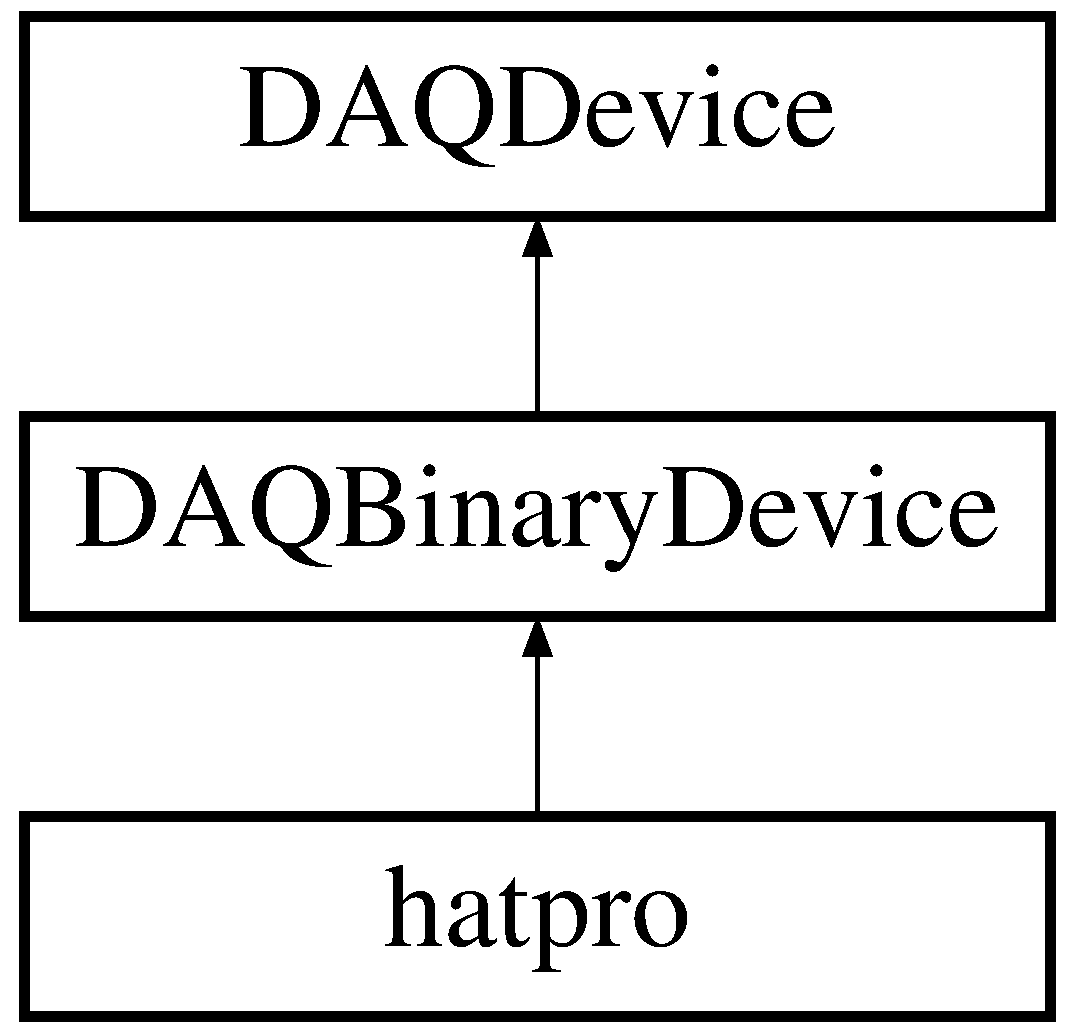
\includegraphics[height=3.000000cm]{classhatpro}
\end{center}
\end{figure}
\subsection*{Public Member Functions}
\begin{DoxyCompactItemize}
\item 
\hyperlink{classhatpro_aa708fafc960ee885b4545c2ebfd81780}{hatpro} ()
\item 
\hyperlink{classhatpro_abf2202318c5b00a9a8e1140e2971f112}{$\sim$hatpro} ()
\item 
void \hyperlink{classhatpro_a8d4126b59d1f8c9958b533ff1022f90a}{open\-Database} ()
\item 
int \hyperlink{classhatpro_aa252764179bbe6f3c06b4a02ded7be52}{create\-\_\-data\-\_\-table} ()
\item 
unsigned int \hyperlink{classhatpro_a0bfedca307a0c586e4eaf3ff60ef64a3}{get\-Sensor\-Group} ()
\item 
int \hyperlink{classhatpro_a5122a613dc3fc746347cf221648af619}{read\-Header} (const char $\ast$\hyperlink{classDAQDevice_a7f9cda7cf5b41f6b134c313477e9644b}{filename})
\item 
void \hyperlink{classhatpro_a6a22e73eb5d50f6425d8e46795d2007a}{read\-Data} (std\-::string \hyperlink{classDAQDevice_a7f9cda7cf5b41f6b134c313477e9644b}{filename})
\end{DoxyCompactItemize}
\subsection*{Protected Attributes}
\begin{DoxyCompactItemize}
\item 
int \hyperlink{classhatpro_a6de7c54e88b099087eec558a97b24e64}{n\-Vars}
\item 
int \hyperlink{classhatpro_a59197a83629dd383c55b4d3332ae70d8}{n\-Sensor\-Flat}
\end{DoxyCompactItemize}
\subsection*{Additional Inherited Members}


\subsection{Constructor \& Destructor Documentation}
\hypertarget{classhatpro_aa708fafc960ee885b4545c2ebfd81780}{\index{hatpro@{hatpro}!hatpro@{hatpro}}
\index{hatpro@{hatpro}!hatpro@{hatpro}}
\subsubsection[{hatpro}]{\setlength{\rightskip}{0pt plus 5cm}hatpro\-::hatpro (
\begin{DoxyParamCaption}
{}
\end{DoxyParamCaption}
)}}\label{classhatpro_aa708fafc960ee885b4545c2ebfd81780}
\hypertarget{classhatpro_abf2202318c5b00a9a8e1140e2971f112}{\index{hatpro@{hatpro}!$\sim$hatpro@{$\sim$hatpro}}
\index{$\sim$hatpro@{$\sim$hatpro}!hatpro@{hatpro}}
\subsubsection[{$\sim$hatpro}]{\setlength{\rightskip}{0pt plus 5cm}hatpro\-::$\sim$hatpro (
\begin{DoxyParamCaption}
{}
\end{DoxyParamCaption}
)}}\label{classhatpro_abf2202318c5b00a9a8e1140e2971f112}


\subsection{Member Function Documentation}
\hypertarget{classhatpro_aa252764179bbe6f3c06b4a02ded7be52}{\index{hatpro@{hatpro}!create\-\_\-data\-\_\-table@{create\-\_\-data\-\_\-table}}
\index{create\-\_\-data\-\_\-table@{create\-\_\-data\-\_\-table}!hatpro@{hatpro}}
\subsubsection[{create\-\_\-data\-\_\-table}]{\setlength{\rightskip}{0pt plus 5cm}int hatpro\-::create\-\_\-data\-\_\-table (
\begin{DoxyParamCaption}
{}
\end{DoxyParamCaption}
)\hspace{0.3cm}{\ttfamily [virtual]}}}\label{classhatpro_aa252764179bbe6f3c06b4a02ded7be52}
Create data table, if it doesn't exist. The function is called by \hyperlink{classhatpro_a8d4126b59d1f8c9958b533ff1022f90a}{open\-Database()}. 

Reimplemented from \hyperlink{classDAQDevice_ac4867b7e5aff2d5c404d6eb1053dda71}{D\-A\-Q\-Device}.

\hypertarget{classhatpro_a0bfedca307a0c586e4eaf3ff60ef64a3}{\index{hatpro@{hatpro}!get\-Sensor\-Group@{get\-Sensor\-Group}}
\index{get\-Sensor\-Group@{get\-Sensor\-Group}!hatpro@{hatpro}}
\subsubsection[{get\-Sensor\-Group}]{\setlength{\rightskip}{0pt plus 5cm}unsigned int hatpro\-::get\-Sensor\-Group (
\begin{DoxyParamCaption}
{}
\end{DoxyParamCaption}
)\hspace{0.3cm}{\ttfamily [virtual]}}}\label{classhatpro_a0bfedca307a0c586e4eaf3ff60ef64a3}
Return the number of the sensor group 

Reimplemented from \hyperlink{classDAQDevice_a61d08492a11c30944dfaf3b86115abe8}{D\-A\-Q\-Device}.

\hypertarget{classhatpro_a8d4126b59d1f8c9958b533ff1022f90a}{\index{hatpro@{hatpro}!open\-Database@{open\-Database}}
\index{open\-Database@{open\-Database}!hatpro@{hatpro}}
\subsubsection[{open\-Database}]{\setlength{\rightskip}{0pt plus 5cm}void hatpro\-::open\-Database (
\begin{DoxyParamCaption}
{}
\end{DoxyParamCaption}
)\hspace{0.3cm}{\ttfamily [virtual]}}}\label{classhatpro_a8d4126b59d1f8c9958b533ff1022f90a}
Open the database and create all required tables The required tables are axislist, sensorlist, statuslist and the data table for the current D\-A\-Q device. 

Reimplemented from \hyperlink{classDAQDevice_a32f118d291f1c7b8fe47a16474b825e2}{D\-A\-Q\-Device}.

\hypertarget{classhatpro_a6a22e73eb5d50f6425d8e46795d2007a}{\index{hatpro@{hatpro}!read\-Data@{read\-Data}}
\index{read\-Data@{read\-Data}!hatpro@{hatpro}}
\subsubsection[{read\-Data}]{\setlength{\rightskip}{0pt plus 5cm}void hatpro\-::read\-Data (
\begin{DoxyParamCaption}
\item[{std\-::string}]{filename}
\end{DoxyParamCaption}
)\hspace{0.3cm}{\ttfamily [virtual]}}}\label{classhatpro_a6a22e73eb5d50f6425d8e46795d2007a}


Reimplemented from \hyperlink{classDAQBinaryDevice_a725281822b7945b8c1154d079c0011ff}{D\-A\-Q\-Binary\-Device}.

\hypertarget{classhatpro_a5122a613dc3fc746347cf221648af619}{\index{hatpro@{hatpro}!read\-Header@{read\-Header}}
\index{read\-Header@{read\-Header}!hatpro@{hatpro}}
\subsubsection[{read\-Header}]{\setlength{\rightskip}{0pt plus 5cm}int hatpro\-::read\-Header (
\begin{DoxyParamCaption}
\item[{const char $\ast$}]{header}
\end{DoxyParamCaption}
)\hspace{0.3cm}{\ttfamily [virtual]}}}\label{classhatpro_a5122a613dc3fc746347cf221648af619}
Get time until next sample and it's id 

Reimplemented from \hyperlink{classDAQDevice_af5fa373af9a089c18c7fd1d662db144f}{D\-A\-Q\-Device}.



\subsection{Member Data Documentation}
\hypertarget{classhatpro_a59197a83629dd383c55b4d3332ae70d8}{\index{hatpro@{hatpro}!n\-Sensor\-Flat@{n\-Sensor\-Flat}}
\index{n\-Sensor\-Flat@{n\-Sensor\-Flat}!hatpro@{hatpro}}
\subsubsection[{n\-Sensor\-Flat}]{\setlength{\rightskip}{0pt plus 5cm}int hatpro\-::n\-Sensor\-Flat\hspace{0.3cm}{\ttfamily [protected]}}}\label{classhatpro_a59197a83629dd383c55b4d3332ae70d8}
\hypertarget{classhatpro_a6de7c54e88b099087eec558a97b24e64}{\index{hatpro@{hatpro}!n\-Vars@{n\-Vars}}
\index{n\-Vars@{n\-Vars}!hatpro@{hatpro}}
\subsubsection[{n\-Vars}]{\setlength{\rightskip}{0pt plus 5cm}int hatpro\-::n\-Vars\hspace{0.3cm}{\ttfamily [protected]}}}\label{classhatpro_a6de7c54e88b099087eec558a97b24e64}


The documentation for this class was generated from the following files\-:\begin{DoxyCompactItemize}
\item 
/home/ntj/\-Development/phd/kitcube-\/tools/src/kitcube-\/devices/\hyperlink{hatpro_8h}{hatpro.\-h}\item 
/home/ntj/\-Development/phd/kitcube-\/tools/src/kitcube-\/devices/\hyperlink{hatpro_8cpp}{hatpro.\-cpp}\end{DoxyCompactItemize}

\hypertarget{classInifile}{\section{Inifile Class Reference}
\label{classInifile}\index{Inifile@{Inifile}}
}


{\ttfamily \#include $<$inifile.\-h$>$}

Inheritance diagram for Inifile\-:\begin{figure}[H]
\begin{center}
\leavevmode
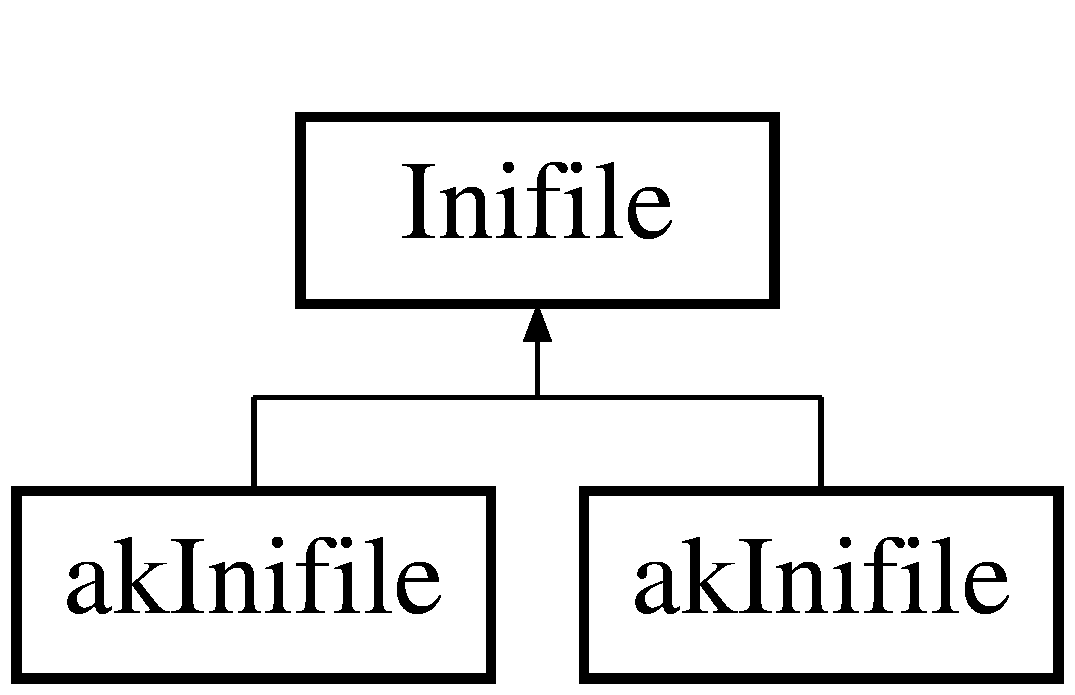
\includegraphics[height=2.000000cm]{classInifile}
\end{center}
\end{figure}
\subsection*{Public Types}
\begin{DoxyCompactItemize}
\item 
enum \hyperlink{classInifile_a42a1cfa6fc8618c8b28d449626f0ecde}{result} \{ \hyperlink{classInifile_a42a1cfa6fc8618c8b28d449626f0ecdeaf094f928f6263c0a635dc56877ada5ee}{k\-F\-A\-I\-L}, 
\hyperlink{classInifile_a42a1cfa6fc8618c8b28d449626f0ecdea729ee722b08e740339d4655b478da609}{k\-S\-U\-C\-C\-E\-S\-S}, 
\hyperlink{classInifile_a42a1cfa6fc8618c8b28d449626f0ecdeaf094f928f6263c0a635dc56877ada5ee}{k\-F\-A\-I\-L}, 
\hyperlink{classInifile_a42a1cfa6fc8618c8b28d449626f0ecdea729ee722b08e740339d4655b478da609}{k\-S\-U\-C\-C\-E\-S\-S}
 \}
\item 
enum \hyperlink{classInifile_a42a1cfa6fc8618c8b28d449626f0ecde}{result} \{ \hyperlink{classInifile_a42a1cfa6fc8618c8b28d449626f0ecdeaf094f928f6263c0a635dc56877ada5ee}{k\-F\-A\-I\-L}, 
\hyperlink{classInifile_a42a1cfa6fc8618c8b28d449626f0ecdea729ee722b08e740339d4655b478da609}{k\-S\-U\-C\-C\-E\-S\-S}, 
\hyperlink{classInifile_a42a1cfa6fc8618c8b28d449626f0ecdeaf094f928f6263c0a635dc56877ada5ee}{k\-F\-A\-I\-L}, 
\hyperlink{classInifile_a42a1cfa6fc8618c8b28d449626f0ecdea729ee722b08e740339d4655b478da609}{k\-S\-U\-C\-C\-E\-S\-S}
 \}
\end{DoxyCompactItemize}
\subsection*{Public Member Functions}
\begin{DoxyCompactItemize}
\item 
\hyperlink{classInifile_a9680323d455ccc8d035d6bf45faea04e}{Inifile} (char $\ast$\-\_\-filename)
\item 
\hyperlink{classInifile_a5b7f8d5c72e6b7c61773e00252ee347d}{$\sim$\-Inifile} ()
\item 
\hyperlink{classInifile_a42a1cfa6fc8618c8b28d449626f0ecde}{result} \hyperlink{classInifile_a0e2952a53275adcf8bcd027365777b25}{Status} ()
\item 
char $\ast$ \hyperlink{classInifile_a778c149a99636e0e73593a5e0dec2f1e}{Get\-Filename} ()
\item 
char $\ast$ \hyperlink{classInifile_a9287991cc2c90c4c8805a26115960671}{Get\-First\-String} (char $\ast$\-\_\-entry)
\item 
int \hyperlink{classInifile_a874d03d73ed88186a79e86fb79876fc9}{Get\-First\-Value} (char $\ast$\-\_\-entry, \hyperlink{classInifile_a42a1cfa6fc8618c8b28d449626f0ecde}{result} $\ast$error=N\-U\-L\-L)
\item 
char $\ast$ \hyperlink{classInifile_ab8462abdac3d6438f9c458c99e2870e0}{Get\-Next\-String} ()
\item 
int \hyperlink{classInifile_a9b1541b9acc9d672190c8d86428647fc}{Get\-Next\-Value} (\hyperlink{classInifile_a42a1cfa6fc8618c8b28d449626f0ecde}{result} $\ast$error=N\-U\-L\-L)
\item 
void \hyperlink{classInifile_a8184de31b799ff84d413c4d474d43c53}{Reset} ()
\item 
\hyperlink{classInifile_a42a1cfa6fc8618c8b28d449626f0ecde}{result} \hyperlink{classInifile_a1a8d8afddf14a50a9efee618a3ca5bec}{Specify\-Group} (char $\ast$string)
\item 
\hyperlink{classInifile_a9680323d455ccc8d035d6bf45faea04e}{Inifile} (char $\ast$\-\_\-filename)
\item 
\hyperlink{classInifile_a5b7f8d5c72e6b7c61773e00252ee347d}{$\sim$\-Inifile} ()
\item 
\hyperlink{classInifile_a42a1cfa6fc8618c8b28d449626f0ecde}{result} \hyperlink{classInifile_a0e2952a53275adcf8bcd027365777b25}{Status} ()
\item 
char $\ast$ \hyperlink{classInifile_a778c149a99636e0e73593a5e0dec2f1e}{Get\-Filename} ()
\item 
char $\ast$ \hyperlink{classInifile_a46088b8c17e7ed51d9cd4434f100efa8}{Get\-First\-String} (char $\ast$\-\_\-entry)
\item 
int \hyperlink{classInifile_a874d03d73ed88186a79e86fb79876fc9}{Get\-First\-Value} (char $\ast$\-\_\-entry, \hyperlink{classInifile_a42a1cfa6fc8618c8b28d449626f0ecde}{result} $\ast$error=N\-U\-L\-L)
\item 
char $\ast$ \hyperlink{classInifile_a4c5de25933bf036015d5117a51c2c1c1}{Get\-Next\-String} ()
\item 
int \hyperlink{classInifile_a9b1541b9acc9d672190c8d86428647fc}{Get\-Next\-Value} (\hyperlink{classInifile_a42a1cfa6fc8618c8b28d449626f0ecde}{result} $\ast$error=N\-U\-L\-L)
\item 
void \hyperlink{classInifile_a8184de31b799ff84d413c4d474d43c53}{Reset} ()
\item 
\hyperlink{classInifile_a42a1cfa6fc8618c8b28d449626f0ecde}{result} \hyperlink{classInifile_a04cdffb13677cd560b1e2aeac74cd200}{Specify\-Group} (char $\ast$string)
\end{DoxyCompactItemize}
\subsection*{Protected Member Functions}
\begin{DoxyCompactItemize}
\item 
char \hyperlink{classInifile_a0ce7414130fe0e8133e050870ac8a64e}{\-\_\-\-Digit2\-Value} (char digit)
\item 
char \hyperlink{classInifile_a44dbf3a265dda32c1575da23ab5c62cc}{\-\_\-\-Digits2\-Value} (char $\ast$$\ast$src, char $\ast$end, int base)
\item 
char \hyperlink{classInifile_ae35b07dd314eba6045b7bbde1fecb654}{\-\_\-\-Get\-Next\-Character} (char $\ast$$\ast$src, char $\ast$end)
\item 
char $\ast$ \hyperlink{classInifile_a9467c2d8a51350310210cbd75faa5522}{\-\_\-\-Get\-Line} ()
\item 
char \hyperlink{classInifile_a0ce7414130fe0e8133e050870ac8a64e}{\-\_\-\-Digit2\-Value} (char digit)
\item 
char \hyperlink{classInifile_a44dbf3a265dda32c1575da23ab5c62cc}{\-\_\-\-Digits2\-Value} (char $\ast$$\ast$src, char $\ast$end, int base)
\item 
char \hyperlink{classInifile_ae35b07dd314eba6045b7bbde1fecb654}{\-\_\-\-Get\-Next\-Character} (char $\ast$$\ast$src, char $\ast$end)
\item 
char $\ast$ \hyperlink{classInifile_a15695f0103c901b9dcece2c29595f911}{\-\_\-\-Get\-Line} ()
\end{DoxyCompactItemize}
\subsection*{Protected Attributes}
\begin{DoxyCompactItemize}
\item 
F\-I\-L\-E $\ast$ \hyperlink{classInifile_ae0124995e028778d1de49eee5cc5eca2}{f\-Inifile}
\item 
char \hyperlink{classInifile_a2be8f61e323dc6a9677952e2bf2e3815}{f\-Linebuf} \mbox{[}\hyperlink{minimal_2inifile_8h_a5d1e6b6f624980109358cdd755f3b3ae}{I\-N\-I\-F\-I\-L\-E\-\_\-\-L\-I\-N\-E\-\_\-\-B\-U\-F\-F\-E\-R\-\_\-\-S\-I\-Z\-E}\mbox{]}
\item 
char $\ast$ \hyperlink{classInifile_af0e8b673a17778eb70b22e35a6b328d2}{f\-Filename}
\item 
char $\ast$ \hyperlink{classInifile_a7a256617578ef60fde020cff47974cf6}{f\-Group}
\item 
char $\ast$ \hyperlink{classInifile_a7742de9155b0368dd608afdddbf679bf}{f\-Lineptr}
\item 
char $\ast$ \hyperlink{classInifile_ab1168d90990e04b72589184377fd07cc}{f\-Ptr}
\item 
int \hyperlink{classInifile_a534bb73b81dea9c6d4c540d6f666c8fc}{f\-Gr\-Pos}
\item 
\hyperlink{classInifile_a42a1cfa6fc8618c8b28d449626f0ecde}{result} \hyperlink{classInifile_a76e65bc01ffe98d10386326bcb814029}{f\-Status}
\end{DoxyCompactItemize}


\subsection{Detailed Description}
Functions to parse a windows like ini file

Changes\-: 8.\-3.\-01 ak\-: Internal preprocessor define pragmas S\-U\-C\-C\-E\-S\-S and F\-A\-I\-L changed to k\-S\-U\-C\-C\-E\-S\-S and K\-F\-A\-I\-L

\begin{DoxyRefDesc}{Todo}
\item[\hyperlink{todo__todo000003}{Todo}]There are warning of not initialized string functions ?!\end{DoxyRefDesc}


Functions to parse a windows like ini file

Changes\-: 8.\-3.\-01 ak\-: Internal preprocessor define pragmas S\-U\-C\-C\-E\-S\-S and F\-A\-I\-L changed to k\-S\-U\-C\-C\-E\-S\-S and K\-F\-A\-I\-L

\begin{DoxyRefDesc}{Todo}
\item[\hyperlink{todo__todo000011}{Todo}]There are warning of not initialized string functions ?!\end{DoxyRefDesc}


\subsection{Member Enumeration Documentation}
\hypertarget{classInifile_a42a1cfa6fc8618c8b28d449626f0ecde}{\index{Inifile@{Inifile}!result@{result}}
\index{result@{result}!Inifile@{Inifile}}
\subsubsection[{result}]{\setlength{\rightskip}{0pt plus 5cm}enum {\bf Inifile\-::result}}}\label{classInifile_a42a1cfa6fc8618c8b28d449626f0ecde}
List of possible results \begin{Desc}
\item[Enumerator]\par
\begin{description}
\index{k\-F\-A\-I\-L@{k\-F\-A\-I\-L}!Inifile@{Inifile}}\index{Inifile@{Inifile}!k\-F\-A\-I\-L@{k\-F\-A\-I\-L}}\item[{\em 
\hypertarget{classInifile_a42a1cfa6fc8618c8b28d449626f0ecdeaf094f928f6263c0a635dc56877ada5ee}{k\-F\-A\-I\-L}\label{classInifile_a42a1cfa6fc8618c8b28d449626f0ecdeaf094f928f6263c0a635dc56877ada5ee}
}]\index{k\-S\-U\-C\-C\-E\-S\-S@{k\-S\-U\-C\-C\-E\-S\-S}!Inifile@{Inifile}}\index{Inifile@{Inifile}!k\-S\-U\-C\-C\-E\-S\-S@{k\-S\-U\-C\-C\-E\-S\-S}}\item[{\em 
\hypertarget{classInifile_a42a1cfa6fc8618c8b28d449626f0ecdea729ee722b08e740339d4655b478da609}{k\-S\-U\-C\-C\-E\-S\-S}\label{classInifile_a42a1cfa6fc8618c8b28d449626f0ecdea729ee722b08e740339d4655b478da609}
}]\index{k\-F\-A\-I\-L@{k\-F\-A\-I\-L}!Inifile@{Inifile}}\index{Inifile@{Inifile}!k\-F\-A\-I\-L@{k\-F\-A\-I\-L}}\item[{\em 
\hypertarget{classInifile_a42a1cfa6fc8618c8b28d449626f0ecdeaf094f928f6263c0a635dc56877ada5ee}{k\-F\-A\-I\-L}\label{classInifile_a42a1cfa6fc8618c8b28d449626f0ecdeaf094f928f6263c0a635dc56877ada5ee}
}]\index{k\-S\-U\-C\-C\-E\-S\-S@{k\-S\-U\-C\-C\-E\-S\-S}!Inifile@{Inifile}}\index{Inifile@{Inifile}!k\-S\-U\-C\-C\-E\-S\-S@{k\-S\-U\-C\-C\-E\-S\-S}}\item[{\em 
\hypertarget{classInifile_a42a1cfa6fc8618c8b28d449626f0ecdea729ee722b08e740339d4655b478da609}{k\-S\-U\-C\-C\-E\-S\-S}\label{classInifile_a42a1cfa6fc8618c8b28d449626f0ecdea729ee722b08e740339d4655b478da609}
}]\end{description}
\end{Desc}
\hypertarget{classInifile_a42a1cfa6fc8618c8b28d449626f0ecde}{\index{Inifile@{Inifile}!result@{result}}
\index{result@{result}!Inifile@{Inifile}}
\subsubsection[{result}]{\setlength{\rightskip}{0pt plus 5cm}enum {\bf Inifile\-::result}}}\label{classInifile_a42a1cfa6fc8618c8b28d449626f0ecde}
List of possible results \begin{Desc}
\item[Enumerator]\par
\begin{description}
\index{k\-F\-A\-I\-L@{k\-F\-A\-I\-L}!Inifile@{Inifile}}\index{Inifile@{Inifile}!k\-F\-A\-I\-L@{k\-F\-A\-I\-L}}\item[{\em 
\hypertarget{classInifile_a42a1cfa6fc8618c8b28d449626f0ecdeaf094f928f6263c0a635dc56877ada5ee}{k\-F\-A\-I\-L}\label{classInifile_a42a1cfa6fc8618c8b28d449626f0ecdeaf094f928f6263c0a635dc56877ada5ee}
}]\index{k\-S\-U\-C\-C\-E\-S\-S@{k\-S\-U\-C\-C\-E\-S\-S}!Inifile@{Inifile}}\index{Inifile@{Inifile}!k\-S\-U\-C\-C\-E\-S\-S@{k\-S\-U\-C\-C\-E\-S\-S}}\item[{\em 
\hypertarget{classInifile_a42a1cfa6fc8618c8b28d449626f0ecdea729ee722b08e740339d4655b478da609}{k\-S\-U\-C\-C\-E\-S\-S}\label{classInifile_a42a1cfa6fc8618c8b28d449626f0ecdea729ee722b08e740339d4655b478da609}
}]\index{k\-F\-A\-I\-L@{k\-F\-A\-I\-L}!Inifile@{Inifile}}\index{Inifile@{Inifile}!k\-F\-A\-I\-L@{k\-F\-A\-I\-L}}\item[{\em 
\hypertarget{classInifile_a42a1cfa6fc8618c8b28d449626f0ecdeaf094f928f6263c0a635dc56877ada5ee}{k\-F\-A\-I\-L}\label{classInifile_a42a1cfa6fc8618c8b28d449626f0ecdeaf094f928f6263c0a635dc56877ada5ee}
}]\index{k\-S\-U\-C\-C\-E\-S\-S@{k\-S\-U\-C\-C\-E\-S\-S}!Inifile@{Inifile}}\index{Inifile@{Inifile}!k\-S\-U\-C\-C\-E\-S\-S@{k\-S\-U\-C\-C\-E\-S\-S}}\item[{\em 
\hypertarget{classInifile_a42a1cfa6fc8618c8b28d449626f0ecdea729ee722b08e740339d4655b478da609}{k\-S\-U\-C\-C\-E\-S\-S}\label{classInifile_a42a1cfa6fc8618c8b28d449626f0ecdea729ee722b08e740339d4655b478da609}
}]\end{description}
\end{Desc}


\subsection{Constructor \& Destructor Documentation}
\hypertarget{classInifile_a9680323d455ccc8d035d6bf45faea04e}{\index{Inifile@{Inifile}!Inifile@{Inifile}}
\index{Inifile@{Inifile}!Inifile@{Inifile}}
\subsubsection[{Inifile}]{\setlength{\rightskip}{0pt plus 5cm}Inifile\-::\-Inifile (
\begin{DoxyParamCaption}
\item[{char $\ast$}]{filename}
\end{DoxyParamCaption}
)}}\label{classInifile_a9680323d455ccc8d035d6bf45faea04e}
example \-:

Let us assume the following entry in a file named \char`\"{}address.\-ini\char`\"{}

\mbox{[}Thomas\mbox{]}

weight= 80

city= 76137 Karlsruhe

\mbox{[}Helmut\mbox{]}

weight= 280

city= 67137 Oggersheim

If we want to get the post code and the town in the group \mbox{[}Thomas\mbox{]}

we have to call the following instructions\-:

specify file\-:

Open\-Ini\-File (\char`\"{}address.\-ini\char`\"{});

specify group (groups are indicated by brackets \mbox{[}\mbox{]})\-:

Specify\-Group (\char`\"{}\-Thomas\char`\"{});

getting first entry for \char`\"{}city\char`\"{} as an integer value

The argument \char`\"{}city\char`\"{} only has to be passed to get the first entry.

code = Get\-First\-Value(\char`\"{}city\char`\"{}); -\/$>$ 76137

getting next entry as a string

strcpy (city, \hyperlink{classInifile_ab8462abdac3d6438f9c458c99e2870e0}{Get\-Next\-String()}); -\/$>$ \char`\"{}\-Karlsruhe\char`\"{}

closing file\-:

Close\-Ini\-File ();

note \-:

An occuring '\textbackslash{}' means skipping to next line and appending it. \hypertarget{classInifile_a5b7f8d5c72e6b7c61773e00252ee347d}{\index{Inifile@{Inifile}!$\sim$\-Inifile@{$\sim$\-Inifile}}
\index{$\sim$\-Inifile@{$\sim$\-Inifile}!Inifile@{Inifile}}
\subsubsection[{$\sim$\-Inifile}]{\setlength{\rightskip}{0pt plus 5cm}Inifile\-::$\sim$\-Inifile (
\begin{DoxyParamCaption}
{}
\end{DoxyParamCaption}
)}}\label{classInifile_a5b7f8d5c72e6b7c61773e00252ee347d}
\hypertarget{classInifile_a9680323d455ccc8d035d6bf45faea04e}{\index{Inifile@{Inifile}!Inifile@{Inifile}}
\index{Inifile@{Inifile}!Inifile@{Inifile}}
\subsubsection[{Inifile}]{\setlength{\rightskip}{0pt plus 5cm}Inifile\-::\-Inifile (
\begin{DoxyParamCaption}
\item[{char $\ast$}]{\-\_\-filename}
\end{DoxyParamCaption}
)}}\label{classInifile_a9680323d455ccc8d035d6bf45faea04e}
\hypertarget{classInifile_a5b7f8d5c72e6b7c61773e00252ee347d}{\index{Inifile@{Inifile}!$\sim$\-Inifile@{$\sim$\-Inifile}}
\index{$\sim$\-Inifile@{$\sim$\-Inifile}!Inifile@{Inifile}}
\subsubsection[{$\sim$\-Inifile}]{\setlength{\rightskip}{0pt plus 5cm}Inifile\-::$\sim$\-Inifile (
\begin{DoxyParamCaption}
{}
\end{DoxyParamCaption}
)}}\label{classInifile_a5b7f8d5c72e6b7c61773e00252ee347d}


\subsection{Member Function Documentation}
\hypertarget{classInifile_a0ce7414130fe0e8133e050870ac8a64e}{\index{Inifile@{Inifile}!\-\_\-\-Digit2\-Value@{\-\_\-\-Digit2\-Value}}
\index{\-\_\-\-Digit2\-Value@{\-\_\-\-Digit2\-Value}!Inifile@{Inifile}}
\subsubsection[{\-\_\-\-Digit2\-Value}]{\setlength{\rightskip}{0pt plus 5cm}char Inifile\-::\-\_\-\-Digit2\-Value (
\begin{DoxyParamCaption}
\item[{char}]{digit}
\end{DoxyParamCaption}
)\hspace{0.3cm}{\ttfamily [protected]}}}\label{classInifile_a0ce7414130fe0e8133e050870ac8a64e}
\hypertarget{classInifile_a0ce7414130fe0e8133e050870ac8a64e}{\index{Inifile@{Inifile}!\-\_\-\-Digit2\-Value@{\-\_\-\-Digit2\-Value}}
\index{\-\_\-\-Digit2\-Value@{\-\_\-\-Digit2\-Value}!Inifile@{Inifile}}
\subsubsection[{\-\_\-\-Digit2\-Value}]{\setlength{\rightskip}{0pt plus 5cm}char Inifile\-::\-\_\-\-Digit2\-Value (
\begin{DoxyParamCaption}
\item[{char}]{digit}
\end{DoxyParamCaption}
)\hspace{0.3cm}{\ttfamily [protected]}}}\label{classInifile_a0ce7414130fe0e8133e050870ac8a64e}
\hypertarget{classInifile_a44dbf3a265dda32c1575da23ab5c62cc}{\index{Inifile@{Inifile}!\-\_\-\-Digits2\-Value@{\-\_\-\-Digits2\-Value}}
\index{\-\_\-\-Digits2\-Value@{\-\_\-\-Digits2\-Value}!Inifile@{Inifile}}
\subsubsection[{\-\_\-\-Digits2\-Value}]{\setlength{\rightskip}{0pt plus 5cm}char Inifile\-::\-\_\-\-Digits2\-Value (
\begin{DoxyParamCaption}
\item[{char $\ast$$\ast$}]{src, }
\item[{char $\ast$}]{end, }
\item[{int}]{base}
\end{DoxyParamCaption}
)\hspace{0.3cm}{\ttfamily [protected]}}}\label{classInifile_a44dbf3a265dda32c1575da23ab5c62cc}
\hypertarget{classInifile_a44dbf3a265dda32c1575da23ab5c62cc}{\index{Inifile@{Inifile}!\-\_\-\-Digits2\-Value@{\-\_\-\-Digits2\-Value}}
\index{\-\_\-\-Digits2\-Value@{\-\_\-\-Digits2\-Value}!Inifile@{Inifile}}
\subsubsection[{\-\_\-\-Digits2\-Value}]{\setlength{\rightskip}{0pt plus 5cm}char Inifile\-::\-\_\-\-Digits2\-Value (
\begin{DoxyParamCaption}
\item[{char $\ast$$\ast$}]{src, }
\item[{char $\ast$}]{end, }
\item[{int}]{base}
\end{DoxyParamCaption}
)\hspace{0.3cm}{\ttfamily [protected]}}}\label{classInifile_a44dbf3a265dda32c1575da23ab5c62cc}
\hypertarget{classInifile_a9467c2d8a51350310210cbd75faa5522}{\index{Inifile@{Inifile}!\-\_\-\-Get\-Line@{\-\_\-\-Get\-Line}}
\index{\-\_\-\-Get\-Line@{\-\_\-\-Get\-Line}!Inifile@{Inifile}}
\subsubsection[{\-\_\-\-Get\-Line}]{\setlength{\rightskip}{0pt plus 5cm}char $\ast$ Inifile\-::\-\_\-\-Get\-Line (
\begin{DoxyParamCaption}
{}
\end{DoxyParamCaption}
)\hspace{0.3cm}{\ttfamily [protected]}}}\label{classInifile_a9467c2d8a51350310210cbd75faa5522}
\hypertarget{classInifile_a15695f0103c901b9dcece2c29595f911}{\index{Inifile@{Inifile}!\-\_\-\-Get\-Line@{\-\_\-\-Get\-Line}}
\index{\-\_\-\-Get\-Line@{\-\_\-\-Get\-Line}!Inifile@{Inifile}}
\subsubsection[{\-\_\-\-Get\-Line}]{\setlength{\rightskip}{0pt plus 5cm}char$\ast$ Inifile\-::\-\_\-\-Get\-Line (
\begin{DoxyParamCaption}
{}
\end{DoxyParamCaption}
)\hspace{0.3cm}{\ttfamily [protected]}}}\label{classInifile_a15695f0103c901b9dcece2c29595f911}
\hypertarget{classInifile_ae35b07dd314eba6045b7bbde1fecb654}{\index{Inifile@{Inifile}!\-\_\-\-Get\-Next\-Character@{\-\_\-\-Get\-Next\-Character}}
\index{\-\_\-\-Get\-Next\-Character@{\-\_\-\-Get\-Next\-Character}!Inifile@{Inifile}}
\subsubsection[{\-\_\-\-Get\-Next\-Character}]{\setlength{\rightskip}{0pt plus 5cm}char Inifile\-::\-\_\-\-Get\-Next\-Character (
\begin{DoxyParamCaption}
\item[{char $\ast$$\ast$}]{src, }
\item[{char $\ast$}]{end}
\end{DoxyParamCaption}
)\hspace{0.3cm}{\ttfamily [protected]}}}\label{classInifile_ae35b07dd314eba6045b7bbde1fecb654}
\hypertarget{classInifile_ae35b07dd314eba6045b7bbde1fecb654}{\index{Inifile@{Inifile}!\-\_\-\-Get\-Next\-Character@{\-\_\-\-Get\-Next\-Character}}
\index{\-\_\-\-Get\-Next\-Character@{\-\_\-\-Get\-Next\-Character}!Inifile@{Inifile}}
\subsubsection[{\-\_\-\-Get\-Next\-Character}]{\setlength{\rightskip}{0pt plus 5cm}char Inifile\-::\-\_\-\-Get\-Next\-Character (
\begin{DoxyParamCaption}
\item[{char $\ast$$\ast$}]{src, }
\item[{char $\ast$}]{end}
\end{DoxyParamCaption}
)\hspace{0.3cm}{\ttfamily [protected]}}}\label{classInifile_ae35b07dd314eba6045b7bbde1fecb654}
\hypertarget{classInifile_a778c149a99636e0e73593a5e0dec2f1e}{\index{Inifile@{Inifile}!Get\-Filename@{Get\-Filename}}
\index{Get\-Filename@{Get\-Filename}!Inifile@{Inifile}}
\subsubsection[{Get\-Filename}]{\setlength{\rightskip}{0pt plus 5cm}char$\ast$ Inifile\-::\-Get\-Filename (
\begin{DoxyParamCaption}
{}
\end{DoxyParamCaption}
)\hspace{0.3cm}{\ttfamily [inline]}}}\label{classInifile_a778c149a99636e0e73593a5e0dec2f1e}
\hypertarget{classInifile_a778c149a99636e0e73593a5e0dec2f1e}{\index{Inifile@{Inifile}!Get\-Filename@{Get\-Filename}}
\index{Get\-Filename@{Get\-Filename}!Inifile@{Inifile}}
\subsubsection[{Get\-Filename}]{\setlength{\rightskip}{0pt plus 5cm}char$\ast$ Inifile\-::\-Get\-Filename (
\begin{DoxyParamCaption}
{}
\end{DoxyParamCaption}
)\hspace{0.3cm}{\ttfamily [inline]}}}\label{classInifile_a778c149a99636e0e73593a5e0dec2f1e}
\hypertarget{classInifile_a9287991cc2c90c4c8805a26115960671}{\index{Inifile@{Inifile}!Get\-First\-String@{Get\-First\-String}}
\index{Get\-First\-String@{Get\-First\-String}!Inifile@{Inifile}}
\subsubsection[{Get\-First\-String}]{\setlength{\rightskip}{0pt plus 5cm}char $\ast$ Inifile\-::\-Get\-First\-String (
\begin{DoxyParamCaption}
\item[{char $\ast$}]{\-\_\-entry}
\end{DoxyParamCaption}
)}}\label{classInifile_a9287991cc2c90c4c8805a26115960671}
\hypertarget{classInifile_a46088b8c17e7ed51d9cd4434f100efa8}{\index{Inifile@{Inifile}!Get\-First\-String@{Get\-First\-String}}
\index{Get\-First\-String@{Get\-First\-String}!Inifile@{Inifile}}
\subsubsection[{Get\-First\-String}]{\setlength{\rightskip}{0pt plus 5cm}char$\ast$ Inifile\-::\-Get\-First\-String (
\begin{DoxyParamCaption}
\item[{char $\ast$}]{\-\_\-entry}
\end{DoxyParamCaption}
)}}\label{classInifile_a46088b8c17e7ed51d9cd4434f100efa8}
\hypertarget{classInifile_a874d03d73ed88186a79e86fb79876fc9}{\index{Inifile@{Inifile}!Get\-First\-Value@{Get\-First\-Value}}
\index{Get\-First\-Value@{Get\-First\-Value}!Inifile@{Inifile}}
\subsubsection[{Get\-First\-Value}]{\setlength{\rightskip}{0pt plus 5cm}int Inifile\-::\-Get\-First\-Value (
\begin{DoxyParamCaption}
\item[{char $\ast$}]{\-\_\-entry, }
\item[{{\bf result} $\ast$}]{error = {\ttfamily NULL}}
\end{DoxyParamCaption}
)}}\label{classInifile_a874d03d73ed88186a79e86fb79876fc9}
\hypertarget{classInifile_a874d03d73ed88186a79e86fb79876fc9}{\index{Inifile@{Inifile}!Get\-First\-Value@{Get\-First\-Value}}
\index{Get\-First\-Value@{Get\-First\-Value}!Inifile@{Inifile}}
\subsubsection[{Get\-First\-Value}]{\setlength{\rightskip}{0pt plus 5cm}int Inifile\-::\-Get\-First\-Value (
\begin{DoxyParamCaption}
\item[{char $\ast$}]{\-\_\-entry, }
\item[{{\bf result} $\ast$}]{error = {\ttfamily NULL}}
\end{DoxyParamCaption}
)}}\label{classInifile_a874d03d73ed88186a79e86fb79876fc9}
\hypertarget{classInifile_a4c5de25933bf036015d5117a51c2c1c1}{\index{Inifile@{Inifile}!Get\-Next\-String@{Get\-Next\-String}}
\index{Get\-Next\-String@{Get\-Next\-String}!Inifile@{Inifile}}
\subsubsection[{Get\-Next\-String}]{\setlength{\rightskip}{0pt plus 5cm}char$\ast$ Inifile\-::\-Get\-Next\-String (
\begin{DoxyParamCaption}
{}
\end{DoxyParamCaption}
)}}\label{classInifile_a4c5de25933bf036015d5117a51c2c1c1}
\hypertarget{classInifile_ab8462abdac3d6438f9c458c99e2870e0}{\index{Inifile@{Inifile}!Get\-Next\-String@{Get\-Next\-String}}
\index{Get\-Next\-String@{Get\-Next\-String}!Inifile@{Inifile}}
\subsubsection[{Get\-Next\-String}]{\setlength{\rightskip}{0pt plus 5cm}char $\ast$ Inifile\-::\-Get\-Next\-String (
\begin{DoxyParamCaption}
\item[{void}]{}
\end{DoxyParamCaption}
)}}\label{classInifile_ab8462abdac3d6438f9c458c99e2870e0}
\hypertarget{classInifile_a9b1541b9acc9d672190c8d86428647fc}{\index{Inifile@{Inifile}!Get\-Next\-Value@{Get\-Next\-Value}}
\index{Get\-Next\-Value@{Get\-Next\-Value}!Inifile@{Inifile}}
\subsubsection[{Get\-Next\-Value}]{\setlength{\rightskip}{0pt plus 5cm}int Inifile\-::\-Get\-Next\-Value (
\begin{DoxyParamCaption}
\item[{{\bf result} $\ast$}]{error = {\ttfamily NULL}}
\end{DoxyParamCaption}
)}}\label{classInifile_a9b1541b9acc9d672190c8d86428647fc}
\hypertarget{classInifile_a9b1541b9acc9d672190c8d86428647fc}{\index{Inifile@{Inifile}!Get\-Next\-Value@{Get\-Next\-Value}}
\index{Get\-Next\-Value@{Get\-Next\-Value}!Inifile@{Inifile}}
\subsubsection[{Get\-Next\-Value}]{\setlength{\rightskip}{0pt plus 5cm}int Inifile\-::\-Get\-Next\-Value (
\begin{DoxyParamCaption}
\item[{{\bf result} $\ast$}]{error = {\ttfamily NULL}}
\end{DoxyParamCaption}
)}}\label{classInifile_a9b1541b9acc9d672190c8d86428647fc}
\hypertarget{classInifile_a8184de31b799ff84d413c4d474d43c53}{\index{Inifile@{Inifile}!Reset@{Reset}}
\index{Reset@{Reset}!Inifile@{Inifile}}
\subsubsection[{Reset}]{\setlength{\rightskip}{0pt plus 5cm}void Inifile\-::\-Reset (
\begin{DoxyParamCaption}
{}
\end{DoxyParamCaption}
)}}\label{classInifile_a8184de31b799ff84d413c4d474d43c53}
\hypertarget{classInifile_a8184de31b799ff84d413c4d474d43c53}{\index{Inifile@{Inifile}!Reset@{Reset}}
\index{Reset@{Reset}!Inifile@{Inifile}}
\subsubsection[{Reset}]{\setlength{\rightskip}{0pt plus 5cm}void Inifile\-::\-Reset (
\begin{DoxyParamCaption}
{}
\end{DoxyParamCaption}
)}}\label{classInifile_a8184de31b799ff84d413c4d474d43c53}
\hypertarget{classInifile_a1a8d8afddf14a50a9efee618a3ca5bec}{\index{Inifile@{Inifile}!Specify\-Group@{Specify\-Group}}
\index{Specify\-Group@{Specify\-Group}!Inifile@{Inifile}}
\subsubsection[{Specify\-Group}]{\setlength{\rightskip}{0pt plus 5cm}{\bf Inifile\-::result} Inifile\-::\-Specify\-Group (
\begin{DoxyParamCaption}
\item[{char $\ast$}]{string}
\end{DoxyParamCaption}
)}}\label{classInifile_a1a8d8afddf14a50a9efee618a3ca5bec}
\hypertarget{classInifile_a04cdffb13677cd560b1e2aeac74cd200}{\index{Inifile@{Inifile}!Specify\-Group@{Specify\-Group}}
\index{Specify\-Group@{Specify\-Group}!Inifile@{Inifile}}
\subsubsection[{Specify\-Group}]{\setlength{\rightskip}{0pt plus 5cm}{\bf result} Inifile\-::\-Specify\-Group (
\begin{DoxyParamCaption}
\item[{char $\ast$}]{string}
\end{DoxyParamCaption}
)}}\label{classInifile_a04cdffb13677cd560b1e2aeac74cd200}
\hypertarget{classInifile_a0e2952a53275adcf8bcd027365777b25}{\index{Inifile@{Inifile}!Status@{Status}}
\index{Status@{Status}!Inifile@{Inifile}}
\subsubsection[{Status}]{\setlength{\rightskip}{0pt plus 5cm}{\bf result} Inifile\-::\-Status (
\begin{DoxyParamCaption}
{}
\end{DoxyParamCaption}
)\hspace{0.3cm}{\ttfamily [inline]}}}\label{classInifile_a0e2952a53275adcf8bcd027365777b25}
\hypertarget{classInifile_a0e2952a53275adcf8bcd027365777b25}{\index{Inifile@{Inifile}!Status@{Status}}
\index{Status@{Status}!Inifile@{Inifile}}
\subsubsection[{Status}]{\setlength{\rightskip}{0pt plus 5cm}{\bf result} Inifile\-::\-Status (
\begin{DoxyParamCaption}
{}
\end{DoxyParamCaption}
)\hspace{0.3cm}{\ttfamily [inline]}}}\label{classInifile_a0e2952a53275adcf8bcd027365777b25}


\subsection{Member Data Documentation}
\hypertarget{classInifile_af0e8b673a17778eb70b22e35a6b328d2}{\index{Inifile@{Inifile}!f\-Filename@{f\-Filename}}
\index{f\-Filename@{f\-Filename}!Inifile@{Inifile}}
\subsubsection[{f\-Filename}]{\setlength{\rightskip}{0pt plus 5cm}char $\ast$ Inifile\-::f\-Filename\hspace{0.3cm}{\ttfamily [protected]}}}\label{classInifile_af0e8b673a17778eb70b22e35a6b328d2}
\hypertarget{classInifile_a7a256617578ef60fde020cff47974cf6}{\index{Inifile@{Inifile}!f\-Group@{f\-Group}}
\index{f\-Group@{f\-Group}!Inifile@{Inifile}}
\subsubsection[{f\-Group}]{\setlength{\rightskip}{0pt plus 5cm}char $\ast$ Inifile\-::f\-Group\hspace{0.3cm}{\ttfamily [protected]}}}\label{classInifile_a7a256617578ef60fde020cff47974cf6}
\hypertarget{classInifile_a534bb73b81dea9c6d4c540d6f666c8fc}{\index{Inifile@{Inifile}!f\-Gr\-Pos@{f\-Gr\-Pos}}
\index{f\-Gr\-Pos@{f\-Gr\-Pos}!Inifile@{Inifile}}
\subsubsection[{f\-Gr\-Pos}]{\setlength{\rightskip}{0pt plus 5cm}int Inifile\-::f\-Gr\-Pos\hspace{0.3cm}{\ttfamily [protected]}}}\label{classInifile_a534bb73b81dea9c6d4c540d6f666c8fc}
\hypertarget{classInifile_ae0124995e028778d1de49eee5cc5eca2}{\index{Inifile@{Inifile}!f\-Inifile@{f\-Inifile}}
\index{f\-Inifile@{f\-Inifile}!Inifile@{Inifile}}
\subsubsection[{f\-Inifile}]{\setlength{\rightskip}{0pt plus 5cm}F\-I\-L\-E $\ast$ Inifile\-::f\-Inifile\hspace{0.3cm}{\ttfamily [protected]}}}\label{classInifile_ae0124995e028778d1de49eee5cc5eca2}
\hypertarget{classInifile_a2be8f61e323dc6a9677952e2bf2e3815}{\index{Inifile@{Inifile}!f\-Linebuf@{f\-Linebuf}}
\index{f\-Linebuf@{f\-Linebuf}!Inifile@{Inifile}}
\subsubsection[{f\-Linebuf}]{\setlength{\rightskip}{0pt plus 5cm}char Inifile\-::f\-Linebuf\hspace{0.3cm}{\ttfamily [protected]}}}\label{classInifile_a2be8f61e323dc6a9677952e2bf2e3815}
\hypertarget{classInifile_a7742de9155b0368dd608afdddbf679bf}{\index{Inifile@{Inifile}!f\-Lineptr@{f\-Lineptr}}
\index{f\-Lineptr@{f\-Lineptr}!Inifile@{Inifile}}
\subsubsection[{f\-Lineptr}]{\setlength{\rightskip}{0pt plus 5cm}char $\ast$ Inifile\-::f\-Lineptr\hspace{0.3cm}{\ttfamily [protected]}}}\label{classInifile_a7742de9155b0368dd608afdddbf679bf}
\hypertarget{classInifile_ab1168d90990e04b72589184377fd07cc}{\index{Inifile@{Inifile}!f\-Ptr@{f\-Ptr}}
\index{f\-Ptr@{f\-Ptr}!Inifile@{Inifile}}
\subsubsection[{f\-Ptr}]{\setlength{\rightskip}{0pt plus 5cm}char $\ast$ Inifile\-::f\-Ptr\hspace{0.3cm}{\ttfamily [protected]}}}\label{classInifile_ab1168d90990e04b72589184377fd07cc}
\hypertarget{classInifile_a76e65bc01ffe98d10386326bcb814029}{\index{Inifile@{Inifile}!f\-Status@{f\-Status}}
\index{f\-Status@{f\-Status}!Inifile@{Inifile}}
\subsubsection[{f\-Status}]{\setlength{\rightskip}{0pt plus 5cm}{\bf result} Inifile\-::f\-Status\hspace{0.3cm}{\ttfamily [protected]}}}\label{classInifile_a76e65bc01ffe98d10386326bcb814029}
k\-S\-U\-C\-C\-E\-S\-S indicates a existing ini-\/file 

The documentation for this class was generated from the following files\-:\begin{DoxyCompactItemize}
\item 
/home/ntj/\-Development/phd/kitcube-\/tools/src/akutil/\hyperlink{inifile_8h}{inifile.\-h}\item 
/home/ntj/\-Development/phd/kitcube-\/tools/src/akutil.\-minimal/\hyperlink{minimal_2inifile_8h}{inifile.\-h}\item 
/home/ntj/\-Development/phd/kitcube-\/tools/src/akutil/\hyperlink{inifile_8cpp}{inifile.\-cpp}\item 
/home/ntj/\-Development/phd/kitcube-\/tools/src/akutil.\-minimal/\hyperlink{minimal_2inifile_8cpp}{inifile.\-cpp}\end{DoxyCompactItemize}

\hypertarget{classjwd}{\section{jwd Class Reference}
\label{classjwd}\index{jwd@{jwd}}
}


{\ttfamily \#include $<$jwd.\-h$>$}

Inheritance diagram for jwd\-:\begin{figure}[H]
\begin{center}
\leavevmode
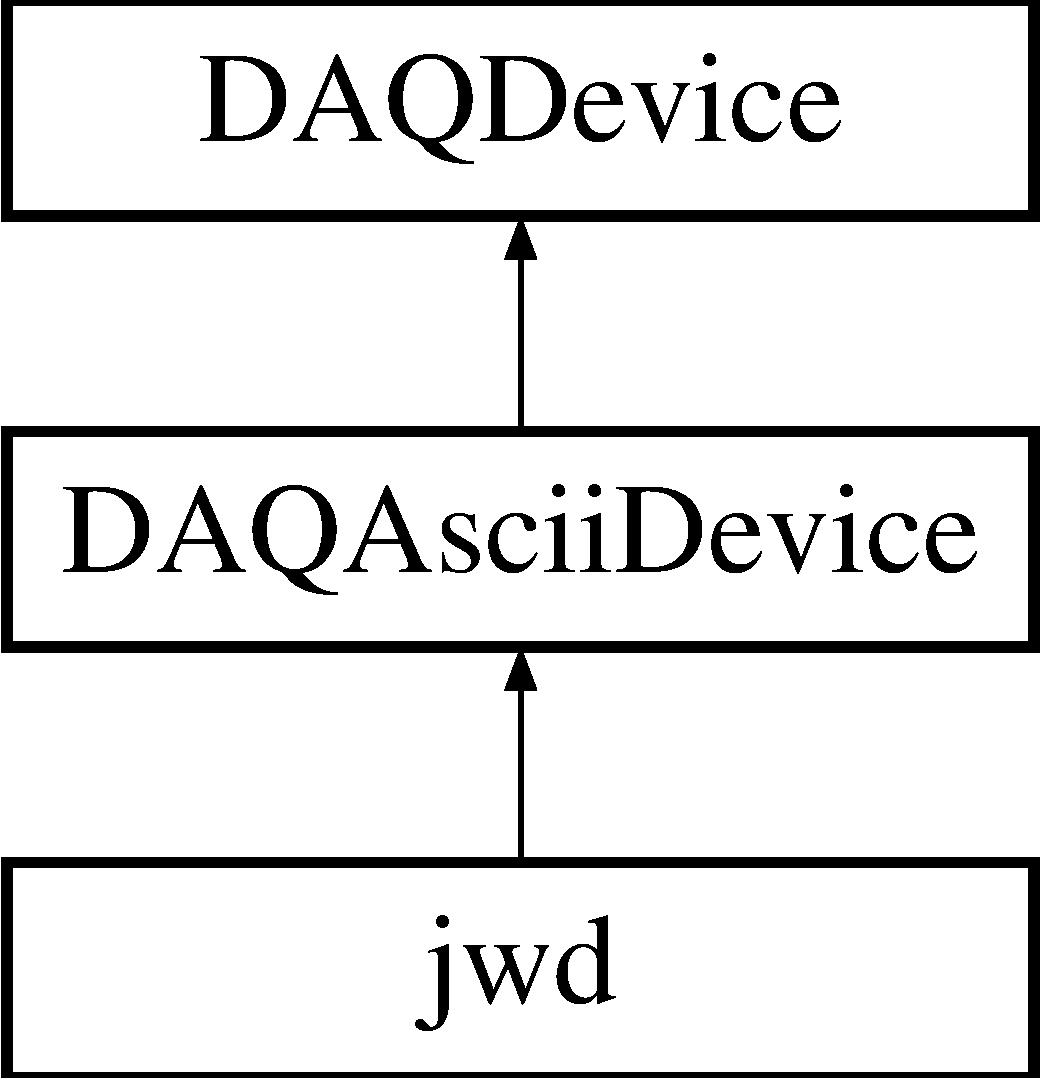
\includegraphics[height=3.000000cm]{classjwd}
\end{center}
\end{figure}
\subsection*{Public Member Functions}
\begin{DoxyCompactItemize}
\item 
\hyperlink{classjwd_a028e5c3cf5dfae165269e8d2afb1930b}{jwd} ()
\item 
\hyperlink{classjwd_a161d08673674ab70d208c78a61bc4b16}{$\sim$jwd} ()
\item 
void \hyperlink{classjwd_ae1e9dc000396fc7078c6300f92f1012e}{set\-Config\-Defaults} ()
\item 
int \hyperlink{classjwd_afb8c407ba5ff5f9c712b11a9bd4a6657}{read\-Header} (const char $\ast$\hyperlink{classDAQDevice_a7f9cda7cf5b41f6b134c313477e9644b}{filename})
\item 
void \hyperlink{classjwd_a51681be8332cc4c174f07e27f5abe594}{write\-Header} ()
\item 
int \hyperlink{classjwd_ae3124d496889e0e756cc9688c4a9a5d7}{parse\-Data} (char $\ast$line, struct timeval $\ast$l\-\_\-t\-Data, double $\ast$\hyperlink{classDAQDevice_ad148188c57598fdf4fd4c1c333aeb0d8}{sensor\-Value})
\item 
void \hyperlink{classjwd_a1476f415afb8ec97f0a5c1dfecf13fc3}{write\-Data} ()
\item 
unsigned int \hyperlink{classjwd_aad72b312ba156e4cd3459121abbf89ef}{get\-Sensor\-Group} ()
\end{DoxyCompactItemize}
\subsection*{Additional Inherited Members}


\subsection{Detailed Description}
Implementation for the weather mast D\-A\-Q devices that are used for turbulence, energy balance and 20m mast. 

\subsection{Constructor \& Destructor Documentation}
\hypertarget{classjwd_a028e5c3cf5dfae165269e8d2afb1930b}{\index{jwd@{jwd}!jwd@{jwd}}
\index{jwd@{jwd}!jwd@{jwd}}
\subsubsection[{jwd}]{\setlength{\rightskip}{0pt plus 5cm}jwd\-::jwd (
\begin{DoxyParamCaption}
{}
\end{DoxyParamCaption}
)}}\label{classjwd_a028e5c3cf5dfae165269e8d2afb1930b}
\hypertarget{classjwd_a161d08673674ab70d208c78a61bc4b16}{\index{jwd@{jwd}!$\sim$jwd@{$\sim$jwd}}
\index{$\sim$jwd@{$\sim$jwd}!jwd@{jwd}}
\subsubsection[{$\sim$jwd}]{\setlength{\rightskip}{0pt plus 5cm}jwd\-::$\sim$jwd (
\begin{DoxyParamCaption}
{}
\end{DoxyParamCaption}
)}}\label{classjwd_a161d08673674ab70d208c78a61bc4b16}


\subsection{Member Function Documentation}
\hypertarget{classjwd_aad72b312ba156e4cd3459121abbf89ef}{\index{jwd@{jwd}!get\-Sensor\-Group@{get\-Sensor\-Group}}
\index{get\-Sensor\-Group@{get\-Sensor\-Group}!jwd@{jwd}}
\subsubsection[{get\-Sensor\-Group}]{\setlength{\rightskip}{0pt plus 5cm}unsigned int jwd\-::get\-Sensor\-Group (
\begin{DoxyParamCaption}
{}
\end{DoxyParamCaption}
)\hspace{0.3cm}{\ttfamily [virtual]}}}\label{classjwd_aad72b312ba156e4cd3459121abbf89ef}
Define a sensor group number for all the availble sensor group files 

Reimplemented from \hyperlink{classDAQDevice_a61d08492a11c30944dfaf3b86115abe8}{D\-A\-Q\-Device}.

\hypertarget{classjwd_ae3124d496889e0e756cc9688c4a9a5d7}{\index{jwd@{jwd}!parse\-Data@{parse\-Data}}
\index{parse\-Data@{parse\-Data}!jwd@{jwd}}
\subsubsection[{parse\-Data}]{\setlength{\rightskip}{0pt plus 5cm}int jwd\-::parse\-Data (
\begin{DoxyParamCaption}
\item[{char $\ast$}]{line, }
\item[{struct timeval $\ast$}]{l\-\_\-t\-Data, }
\item[{double $\ast$}]{sensor\-Value}
\end{DoxyParamCaption}
)\hspace{0.3cm}{\ttfamily [virtual]}}}\label{classjwd_ae3124d496889e0e756cc9688c4a9a5d7}
Read the data from the current line of the data file. \begin{DoxyReturn}{Returns}
-\/1 no data found, skip storage 0 sucess, store data, 1 read another line 
\end{DoxyReturn}


Reimplemented from \hyperlink{classDAQAsciiDevice_a9c20d9d69af4ba1641dbc82dd5be2aa5}{D\-A\-Q\-Ascii\-Device}.

\hypertarget{classjwd_afb8c407ba5ff5f9c712b11a9bd4a6657}{\index{jwd@{jwd}!read\-Header@{read\-Header}}
\index{read\-Header@{read\-Header}!jwd@{jwd}}
\subsubsection[{read\-Header}]{\setlength{\rightskip}{0pt plus 5cm}int jwd\-::read\-Header (
\begin{DoxyParamCaption}
\item[{const char $\ast$}]{header}
\end{DoxyParamCaption}
)\hspace{0.3cm}{\ttfamily [virtual]}}}\label{classjwd_afb8c407ba5ff5f9c712b11a9bd4a6657}
Get time until next sample and it's id 

Reimplemented from \hyperlink{classDAQAsciiDevice_a5fce725c52b70ef2f56a34b32a03e15d}{D\-A\-Q\-Ascii\-Device}.

\hypertarget{classjwd_ae1e9dc000396fc7078c6300f92f1012e}{\index{jwd@{jwd}!set\-Config\-Defaults@{set\-Config\-Defaults}}
\index{set\-Config\-Defaults@{set\-Config\-Defaults}!jwd@{jwd}}
\subsubsection[{set\-Config\-Defaults}]{\setlength{\rightskip}{0pt plus 5cm}void jwd\-::set\-Config\-Defaults (
\begin{DoxyParamCaption}
{}
\end{DoxyParamCaption}
)\hspace{0.3cm}{\ttfamily [virtual]}}}\label{classjwd_ae1e9dc000396fc7078c6300f92f1012e}
The function is called before reading the configuration from the inifile. Use this fucntion in the module specific implementation to override the standard defaults 

Reimplemented from \hyperlink{classDAQDevice_a7685cec80865752cc0ef3ab49c6c2277}{D\-A\-Q\-Device}.

\hypertarget{classjwd_a1476f415afb8ec97f0a5c1dfecf13fc3}{\index{jwd@{jwd}!write\-Data@{write\-Data}}
\index{write\-Data@{write\-Data}!jwd@{jwd}}
\subsubsection[{write\-Data}]{\setlength{\rightskip}{0pt plus 5cm}void jwd\-::write\-Data (
\begin{DoxyParamCaption}
{}
\end{DoxyParamCaption}
)\hspace{0.3cm}{\ttfamily [virtual]}}}\label{classjwd_a1476f415afb8ec97f0a5c1dfecf13fc3}


Reimplemented from \hyperlink{classDAQDevice_acdc9d3765b1dfd845f99ec9c93071811}{D\-A\-Q\-Device}.

\hypertarget{classjwd_a51681be8332cc4c174f07e27f5abe594}{\index{jwd@{jwd}!write\-Header@{write\-Header}}
\index{write\-Header@{write\-Header}!jwd@{jwd}}
\subsubsection[{write\-Header}]{\setlength{\rightskip}{0pt plus 5cm}void jwd\-::write\-Header (
\begin{DoxyParamCaption}
{}
\end{DoxyParamCaption}
)\hspace{0.3cm}{\ttfamily [virtual]}}}\label{classjwd_a51681be8332cc4c174f07e27f5abe594}


Reimplemented from \hyperlink{classDAQDevice_aad39c13f039abd6e6a9b0aa21a7c8a4d}{D\-A\-Q\-Device}.



The documentation for this class was generated from the following files\-:\begin{DoxyCompactItemize}
\item 
/home/ntj/\-Development/phd/kitcube-\/tools/src/kitcube-\/devices/\hyperlink{jwd_8h}{jwd.\-h}\item 
/home/ntj/\-Development/phd/kitcube-\/tools/src/kitcube-\/devices/\hyperlink{jwd_8cpp}{jwd.\-cpp}\end{DoxyCompactItemize}

\hypertarget{classkeyboard}{\section{keyboard Class Reference}
\label{classkeyboard}\index{keyboard@{keyboard}}
}


{\ttfamily \#include $<$keyboard.\-h$>$}

\subsection*{Public Member Functions}
\begin{DoxyCompactItemize}
\item 
\hyperlink{classkeyboard_ac8a026376e79f204ebccd4a0e0eef2f9}{keyboard} ()
\item 
\hyperlink{classkeyboard_a6ee90db5c7b4d44b37724711b6048c34}{$\sim$keyboard} ()
\item 
bool \hyperlink{classkeyboard_acafcfa9baee58ec7f2d5b37995f739f0}{hit} ()
\item 
bool \hyperlink{classkeyboard_a9fc7aa1041b37981a784a9fb750bd355}{hit} (char \hyperlink{classkeyboard_aa38f064c4a946810840ec389c4df81d6}{key})
\item 
char \hyperlink{classkeyboard_a14c52ad4acba6c5b4637ebb8ba2d57fc}{getchar} ()
\item 
char $\ast$ \hyperlink{classkeyboard_ab1be3946c44e55ea5177f077b9f745d6}{getpasswd} ()
\end{DoxyCompactItemize}
\subsection*{Public Attributes}
\begin{DoxyCompactItemize}
\item 
char \hyperlink{classkeyboard_aacee1ab06d08c89eae28515ac52d4333}{passwd} \mbox{[}20\mbox{]}
\end{DoxyCompactItemize}
\subsection*{Private Attributes}
\begin{DoxyCompactItemize}
\item 
char \hyperlink{classkeyboard_aa38f064c4a946810840ec389c4df81d6}{key}
\end{DoxyCompactItemize}


\subsection{Detailed Description}
Emulates the kbhit() function known from

the windows world 

\subsection{Constructor \& Destructor Documentation}
\hypertarget{classkeyboard_ac8a026376e79f204ebccd4a0e0eef2f9}{\index{keyboard@{keyboard}!keyboard@{keyboard}}
\index{keyboard@{keyboard}!keyboard@{keyboard}}
\subsubsection[{keyboard}]{\setlength{\rightskip}{0pt plus 5cm}keyboard\-::keyboard (
\begin{DoxyParamCaption}
{}
\end{DoxyParamCaption}
)\hspace{0.3cm}{\ttfamily [inline]}}}\label{classkeyboard_ac8a026376e79f204ebccd4a0e0eef2f9}
\hypertarget{classkeyboard_a6ee90db5c7b4d44b37724711b6048c34}{\index{keyboard@{keyboard}!$\sim$keyboard@{$\sim$keyboard}}
\index{$\sim$keyboard@{$\sim$keyboard}!keyboard@{keyboard}}
\subsubsection[{$\sim$keyboard}]{\setlength{\rightskip}{0pt plus 5cm}keyboard\-::$\sim$keyboard (
\begin{DoxyParamCaption}
{}
\end{DoxyParamCaption}
)\hspace{0.3cm}{\ttfamily [inline]}}}\label{classkeyboard_a6ee90db5c7b4d44b37724711b6048c34}


\subsection{Member Function Documentation}
\hypertarget{classkeyboard_a14c52ad4acba6c5b4637ebb8ba2d57fc}{\index{keyboard@{keyboard}!getchar@{getchar}}
\index{getchar@{getchar}!keyboard@{keyboard}}
\subsubsection[{getchar}]{\setlength{\rightskip}{0pt plus 5cm}char keyboard\-::getchar (
\begin{DoxyParamCaption}
{}
\end{DoxyParamCaption}
)\hspace{0.3cm}{\ttfamily [inline]}}}\label{classkeyboard_a14c52ad4acba6c5b4637ebb8ba2d57fc}
\hypertarget{classkeyboard_ab1be3946c44e55ea5177f077b9f745d6}{\index{keyboard@{keyboard}!getpasswd@{getpasswd}}
\index{getpasswd@{getpasswd}!keyboard@{keyboard}}
\subsubsection[{getpasswd}]{\setlength{\rightskip}{0pt plus 5cm}char $\ast$ keyboard\-::getpasswd (
\begin{DoxyParamCaption}
{}
\end{DoxyParamCaption}
)\hspace{0.3cm}{\ttfamily [inline]}}}\label{classkeyboard_ab1be3946c44e55ea5177f077b9f745d6}
Read a password from the terminal \hypertarget{classkeyboard_acafcfa9baee58ec7f2d5b37995f739f0}{\index{keyboard@{keyboard}!hit@{hit}}
\index{hit@{hit}!keyboard@{keyboard}}
\subsubsection[{hit}]{\setlength{\rightskip}{0pt plus 5cm}bool keyboard\-::hit (
\begin{DoxyParamCaption}
{}
\end{DoxyParamCaption}
)\hspace{0.3cm}{\ttfamily [inline]}}}\label{classkeyboard_acafcfa9baee58ec7f2d5b37995f739f0}
\hypertarget{classkeyboard_a9fc7aa1041b37981a784a9fb750bd355}{\index{keyboard@{keyboard}!hit@{hit}}
\index{hit@{hit}!keyboard@{keyboard}}
\subsubsection[{hit}]{\setlength{\rightskip}{0pt plus 5cm}bool keyboard\-::hit (
\begin{DoxyParamCaption}
\item[{char}]{key}
\end{DoxyParamCaption}
)\hspace{0.3cm}{\ttfamily [inline]}}}\label{classkeyboard_a9fc7aa1041b37981a784a9fb750bd355}
Returns true if the right key 

\subsection{Member Data Documentation}
\hypertarget{classkeyboard_aa38f064c4a946810840ec389c4df81d6}{\index{keyboard@{keyboard}!key@{key}}
\index{key@{key}!keyboard@{keyboard}}
\subsubsection[{key}]{\setlength{\rightskip}{0pt plus 5cm}char keyboard\-::key\hspace{0.3cm}{\ttfamily [private]}}}\label{classkeyboard_aa38f064c4a946810840ec389c4df81d6}
\hypertarget{classkeyboard_aacee1ab06d08c89eae28515ac52d4333}{\index{keyboard@{keyboard}!passwd@{passwd}}
\index{passwd@{passwd}!keyboard@{keyboard}}
\subsubsection[{passwd}]{\setlength{\rightskip}{0pt plus 5cm}char keyboard\-::passwd\mbox{[}20\mbox{]}}}\label{classkeyboard_aacee1ab06d08c89eae28515ac52d4333}
Character string that contains the last password entered 

The documentation for this class was generated from the following file\-:\begin{DoxyCompactItemize}
\item 
/home/ntj/\-Development/phd/kitcube-\/tools/src/akutil/\hyperlink{keyboard_8h}{keyboard.\-h}\end{DoxyCompactItemize}

\hypertarget{classLara}{\section{Lara Class Reference}
\label{classLara}\index{Lara@{Lara}}
}


{\ttfamily \#include $<$lara.\-h$>$}

Inheritance diagram for Lara\-:\begin{figure}[H]
\begin{center}
\leavevmode
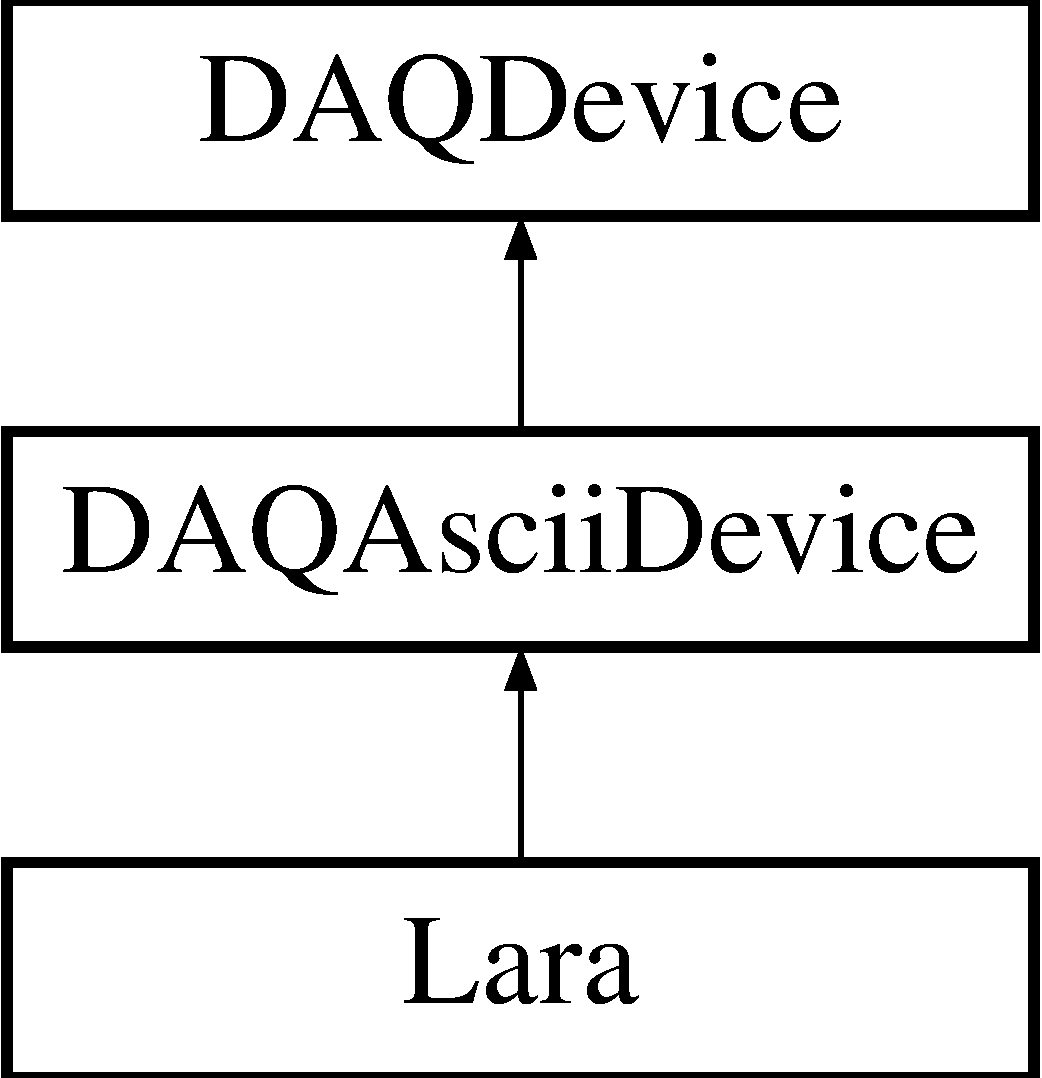
\includegraphics[height=3.000000cm]{classLara}
\end{center}
\end{figure}
\subsection*{Public Member Functions}
\begin{DoxyCompactItemize}
\item 
\hyperlink{classLara_ad6868223e6c8dcec6297e60cf52c0054}{Lara} ()
\item 
\hyperlink{classLara_a13972df0bdfdfc87b69b8e15f4525296}{$\sim$\-Lara} ()
\item 
void \hyperlink{classLara_aa799138169577ef61f0d43341846ccf9}{set\-Config\-Defaults} ()
\item 
const char $\ast$ \hyperlink{classLara_a717b34c0a592c907ead948e010161ba6}{get\-Data\-Dir} ()
\item 
const char $\ast$ \hyperlink{classLara_a91cc9e1a0ac8f8f13b24bcf966524152}{get\-Data\-Filename} ()
\item 
long \hyperlink{classLara_a6061880b0ad621eb863d14eda0ea0b95}{get\-File\-Number} (char $\ast$\hyperlink{classDAQDevice_a7f9cda7cf5b41f6b134c313477e9644b}{filename})
\item 
unsigned int \hyperlink{classLara_a004ffdd20608ea635775b68733a3d5a3}{get\-Sensor\-Group} ()
\item 
int \hyperlink{classLara_af903264894bc1afa28ea3321deeb7083}{read\-Header} (const char $\ast$\hyperlink{classDAQDevice_a7f9cda7cf5b41f6b134c313477e9644b}{filename})
\item 
int \hyperlink{classLara_aff63ff661248c4aa565282eaba084823}{parse\-Data} (char $\ast$line, struct timeval $\ast$l\-\_\-t\-Data, double $\ast$\hyperlink{classDAQDevice_ad148188c57598fdf4fd4c1c333aeb0d8}{sensor\-Value})
\item 
void \hyperlink{classLara_a727b4aa20f48283239922df33c191de1}{read\-Data} (std\-::string full\-\_\-filename)
\item 
void \hyperlink{classLara_abc32ee9688cef1ec84060d3c206c0123}{write\-Data} ()
\end{DoxyCompactItemize}
\subsection*{Private Attributes}
\begin{DoxyCompactItemize}
\item 
struct timeval \hyperlink{classLara_affcaafa6f994ac7ffc6105fdd0571c01}{t\-Ref}
\item 
int \hyperlink{classLara_a5225d610f129a85314440ec529d8b81f}{n\-Template}
\item 
int \hyperlink{classLara_a6ba4f1300d5a85063428df2e100bc6bf}{n\-Samples\-In\-File}
\end{DoxyCompactItemize}
\subsection*{Additional Inherited Members}


\subsection{Detailed Description}
Implementation for the weather mast D\-A\-Q devices that are used for turbulence, energy balance and 20m mast.

\begin{DoxyRefDesc}{Todo}
\item[\hyperlink{todo__todo000016}{Todo}]Implement also storage of the test data in the database The feature should be configurable from the inifile \end{DoxyRefDesc}


\subsection{Constructor \& Destructor Documentation}
\hypertarget{classLara_ad6868223e6c8dcec6297e60cf52c0054}{\index{Lara@{Lara}!Lara@{Lara}}
\index{Lara@{Lara}!Lara@{Lara}}
\subsubsection[{Lara}]{\setlength{\rightskip}{0pt plus 5cm}Lara\-::\-Lara (
\begin{DoxyParamCaption}
{}
\end{DoxyParamCaption}
)}}\label{classLara_ad6868223e6c8dcec6297e60cf52c0054}
\hypertarget{classLara_a13972df0bdfdfc87b69b8e15f4525296}{\index{Lara@{Lara}!$\sim$\-Lara@{$\sim$\-Lara}}
\index{$\sim$\-Lara@{$\sim$\-Lara}!Lara@{Lara}}
\subsubsection[{$\sim$\-Lara}]{\setlength{\rightskip}{0pt plus 5cm}Lara\-::$\sim$\-Lara (
\begin{DoxyParamCaption}
{}
\end{DoxyParamCaption}
)}}\label{classLara_a13972df0bdfdfc87b69b8e15f4525296}


\subsection{Member Function Documentation}
\hypertarget{classLara_a717b34c0a592c907ead948e010161ba6}{\index{Lara@{Lara}!get\-Data\-Dir@{get\-Data\-Dir}}
\index{get\-Data\-Dir@{get\-Data\-Dir}!Lara@{Lara}}
\subsubsection[{get\-Data\-Dir}]{\setlength{\rightskip}{0pt plus 5cm}const char $\ast$ Lara\-::get\-Data\-Dir (
\begin{DoxyParamCaption}
{}
\end{DoxyParamCaption}
)\hspace{0.3cm}{\ttfamily [virtual]}}}\label{classLara_a717b34c0a592c907ead948e010161ba6}


Reimplemented from \hyperlink{classDAQDevice_a7d7d41f0c1496221e589d84b38d1c865}{D\-A\-Q\-Device}.

\hypertarget{classLara_a91cc9e1a0ac8f8f13b24bcf966524152}{\index{Lara@{Lara}!get\-Data\-Filename@{get\-Data\-Filename}}
\index{get\-Data\-Filename@{get\-Data\-Filename}!Lara@{Lara}}
\subsubsection[{get\-Data\-Filename}]{\setlength{\rightskip}{0pt plus 5cm}const char $\ast$ Lara\-::get\-Data\-Filename (
\begin{DoxyParamCaption}
{}
\end{DoxyParamCaption}
)\hspace{0.3cm}{\ttfamily [virtual]}}}\label{classLara_a91cc9e1a0ac8f8f13b24bcf966524152}
Implements the data filename convention of the D\-A\-Q module. 

Reimplemented from \hyperlink{classDAQDevice_af4734900eb86417b3160a723a077f8f5}{D\-A\-Q\-Device}.

\hypertarget{classLara_a6061880b0ad621eb863d14eda0ea0b95}{\index{Lara@{Lara}!get\-File\-Number@{get\-File\-Number}}
\index{get\-File\-Number@{get\-File\-Number}!Lara@{Lara}}
\subsubsection[{get\-File\-Number}]{\setlength{\rightskip}{0pt plus 5cm}long Lara\-::get\-File\-Number (
\begin{DoxyParamCaption}
\item[{char $\ast$}]{filename}
\end{DoxyParamCaption}
)\hspace{0.3cm}{\ttfamily [virtual]}}}\label{classLara_a6061880b0ad621eb863d14eda0ea0b95}
Re-\/implement the calculation of the file numbering scheme. \hyperlink{classLara}{Lara} uses date and times in the filename 

Reimplemented from \hyperlink{classDAQDevice_a56a712062b2b17c6a73cb7fb0a475d2e}{D\-A\-Q\-Device}.

\hypertarget{classLara_a004ffdd20608ea635775b68733a3d5a3}{\index{Lara@{Lara}!get\-Sensor\-Group@{get\-Sensor\-Group}}
\index{get\-Sensor\-Group@{get\-Sensor\-Group}!Lara@{Lara}}
\subsubsection[{get\-Sensor\-Group}]{\setlength{\rightskip}{0pt plus 5cm}unsigned int Lara\-::get\-Sensor\-Group (
\begin{DoxyParamCaption}
{}
\end{DoxyParamCaption}
)\hspace{0.3cm}{\ttfamily [virtual]}}}\label{classLara_a004ffdd20608ea635775b68733a3d5a3}
Define a sensor group number for all the availble sensor group files 

Reimplemented from \hyperlink{classDAQDevice_a61d08492a11c30944dfaf3b86115abe8}{D\-A\-Q\-Device}.

\hypertarget{classLara_aff63ff661248c4aa565282eaba084823}{\index{Lara@{Lara}!parse\-Data@{parse\-Data}}
\index{parse\-Data@{parse\-Data}!Lara@{Lara}}
\subsubsection[{parse\-Data}]{\setlength{\rightskip}{0pt plus 5cm}int Lara\-::parse\-Data (
\begin{DoxyParamCaption}
\item[{char $\ast$}]{line, }
\item[{struct timeval $\ast$}]{l\-\_\-t\-Data, }
\item[{double $\ast$}]{sensor\-Value}
\end{DoxyParamCaption}
)\hspace{0.3cm}{\ttfamily [virtual]}}}\label{classLara_aff63ff661248c4aa565282eaba084823}
Read the data from the current line of the data file. \begin{DoxyReturn}{Returns}
-\/1 no data found, skip storage 0 sucess, store data, 1 read another line 
\end{DoxyReturn}


Reimplemented from \hyperlink{classDAQAsciiDevice_a9c20d9d69af4ba1641dbc82dd5be2aa5}{D\-A\-Q\-Ascii\-Device}.

\hypertarget{classLara_a727b4aa20f48283239922df33c191de1}{\index{Lara@{Lara}!read\-Data@{read\-Data}}
\index{read\-Data@{read\-Data}!Lara@{Lara}}
\subsubsection[{read\-Data}]{\setlength{\rightskip}{0pt plus 5cm}void Lara\-::read\-Data (
\begin{DoxyParamCaption}
\item[{std\-::string}]{full\-\_\-filename}
\end{DoxyParamCaption}
)\hspace{0.3cm}{\ttfamily [virtual]}}}\label{classLara_a727b4aa20f48283239922df33c191de1}


Reimplemented from \hyperlink{classDAQAsciiDevice_a0d9b17803680d966c7025ca6f174cef0}{D\-A\-Q\-Ascii\-Device}.

\hypertarget{classLara_af903264894bc1afa28ea3321deeb7083}{\index{Lara@{Lara}!read\-Header@{read\-Header}}
\index{read\-Header@{read\-Header}!Lara@{Lara}}
\subsubsection[{read\-Header}]{\setlength{\rightskip}{0pt plus 5cm}int Lara\-::read\-Header (
\begin{DoxyParamCaption}
\item[{const char $\ast$}]{filename}
\end{DoxyParamCaption}
)\hspace{0.3cm}{\ttfamily [virtual]}}}\label{classLara_af903264894bc1afa28ea3321deeb7083}
Get time until next sample and it's id 

Reimplemented from \hyperlink{classDAQAsciiDevice_a5fce725c52b70ef2f56a34b32a03e15d}{D\-A\-Q\-Ascii\-Device}.

\hypertarget{classLara_aa799138169577ef61f0d43341846ccf9}{\index{Lara@{Lara}!set\-Config\-Defaults@{set\-Config\-Defaults}}
\index{set\-Config\-Defaults@{set\-Config\-Defaults}!Lara@{Lara}}
\subsubsection[{set\-Config\-Defaults}]{\setlength{\rightskip}{0pt plus 5cm}void Lara\-::set\-Config\-Defaults (
\begin{DoxyParamCaption}
{}
\end{DoxyParamCaption}
)\hspace{0.3cm}{\ttfamily [virtual]}}}\label{classLara_aa799138169577ef61f0d43341846ccf9}
The function is called before reading the configuration from the inifile. Use this fucntion in the module specific implementation to override the standard defaults 

Reimplemented from \hyperlink{classDAQDevice_a7685cec80865752cc0ef3ab49c6c2277}{D\-A\-Q\-Device}.

\hypertarget{classLara_abc32ee9688cef1ec84060d3c206c0123}{\index{Lara@{Lara}!write\-Data@{write\-Data}}
\index{write\-Data@{write\-Data}!Lara@{Lara}}
\subsubsection[{write\-Data}]{\setlength{\rightskip}{0pt plus 5cm}void Lara\-::write\-Data (
\begin{DoxyParamCaption}
{}
\end{DoxyParamCaption}
)\hspace{0.3cm}{\ttfamily [virtual]}}}\label{classLara_abc32ee9688cef1ec84060d3c206c0123}


Reimplemented from \hyperlink{classDAQDevice_acdc9d3765b1dfd845f99ec9c93071811}{D\-A\-Q\-Device}.



\subsection{Member Data Documentation}
\hypertarget{classLara_a6ba4f1300d5a85063428df2e100bc6bf}{\index{Lara@{Lara}!n\-Samples\-In\-File@{n\-Samples\-In\-File}}
\index{n\-Samples\-In\-File@{n\-Samples\-In\-File}!Lara@{Lara}}
\subsubsection[{n\-Samples\-In\-File}]{\setlength{\rightskip}{0pt plus 5cm}int Lara\-::n\-Samples\-In\-File\hspace{0.3cm}{\ttfamily [private]}}}\label{classLara_a6ba4f1300d5a85063428df2e100bc6bf}
Number of samples in one file \hypertarget{classLara_a5225d610f129a85314440ec529d8b81f}{\index{Lara@{Lara}!n\-Template@{n\-Template}}
\index{n\-Template@{n\-Template}!Lara@{Lara}}
\subsubsection[{n\-Template}]{\setlength{\rightskip}{0pt plus 5cm}int Lara\-::n\-Template\hspace{0.3cm}{\ttfamily [private]}}}\label{classLara_a5225d610f129a85314440ec529d8b81f}
\hypertarget{classLara_affcaafa6f994ac7ffc6105fdd0571c01}{\index{Lara@{Lara}!t\-Ref@{t\-Ref}}
\index{t\-Ref@{t\-Ref}!Lara@{Lara}}
\subsubsection[{t\-Ref}]{\setlength{\rightskip}{0pt plus 5cm}struct timeval Lara\-::t\-Ref\hspace{0.3cm}{\ttfamily [private]}}}\label{classLara_affcaafa6f994ac7ffc6105fdd0571c01}


The documentation for this class was generated from the following files\-:\begin{DoxyCompactItemize}
\item 
/home/ntj/\-Development/phd/kitcube-\/tools/src/kitcube-\/devices/\hyperlink{lara_8h}{lara.\-h}\item 
/home/ntj/\-Development/phd/kitcube-\/tools/src/kitcube-\/devices/\hyperlink{lara_8cpp}{lara.\-cpp}\end{DoxyCompactItemize}

\hypertarget{classMast}{\section{Mast Class Reference}
\label{classMast}\index{Mast@{Mast}}
}


{\ttfamily \#include $<$mast.\-h$>$}

Inheritance diagram for Mast\-:\begin{figure}[H]
\begin{center}
\leavevmode
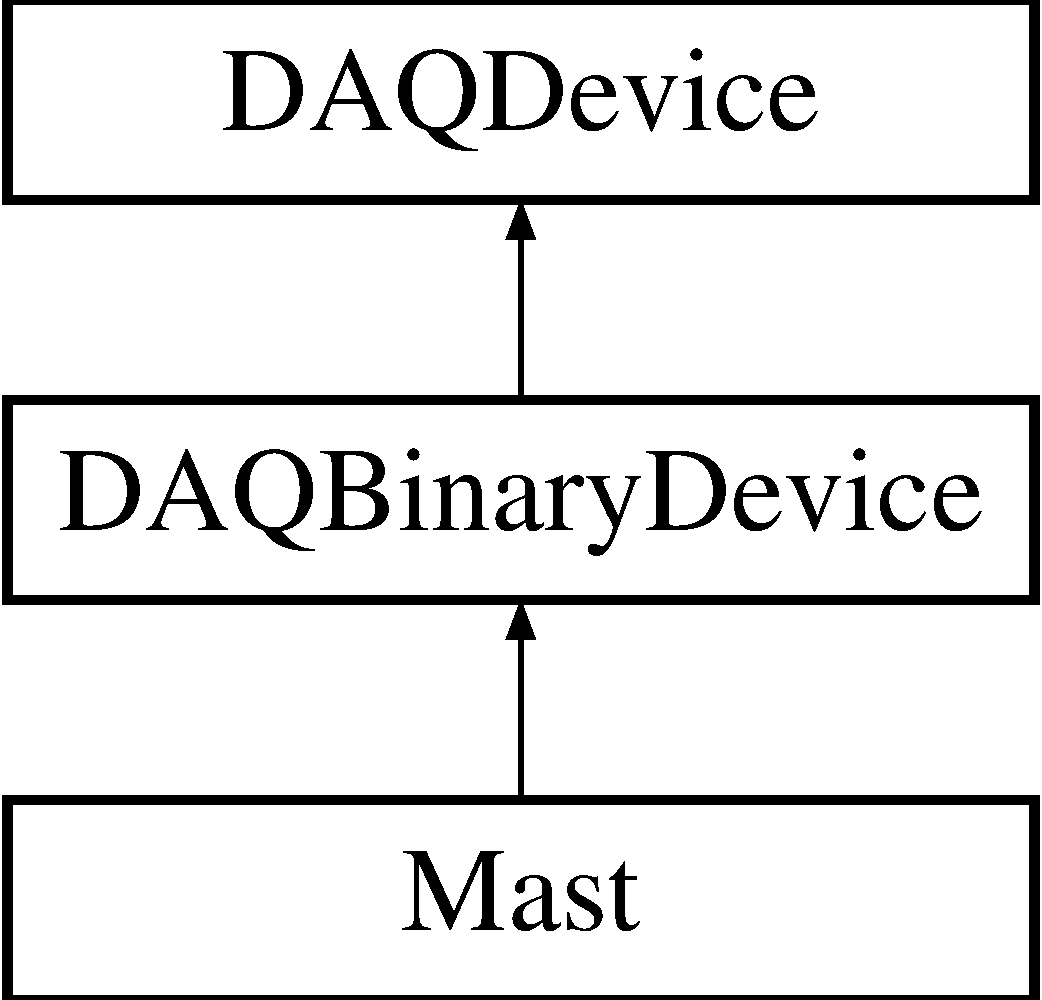
\includegraphics[height=3.000000cm]{classMast}
\end{center}
\end{figure}
\subsection*{Public Member Functions}
\begin{DoxyCompactItemize}
\item 
\hyperlink{classMast_aa398ff904c307faa36b4010e8a9beaaf}{Mast} ()
\item 
\hyperlink{classMast_a1dc94280c9f342657d40d1fb9c4db637}{$\sim$\-Mast} ()
\item 
void \hyperlink{classMast_a0dd0878ebcdb7ef0fe4806cafe4deaff}{set\-Config\-Defaults} ()
\item 
const char $\ast$ \hyperlink{classMast_a728e5f3077a08c7fec100cc8792a1de6}{get\-Data\-Dir} ()
\item 
const char $\ast$ \hyperlink{classMast_af1019b85d2e451e9a57bf9da0638d69e}{get\-Data\-Filename} ()
\item 
void \hyperlink{classMast_a978e895ec47d4566a32e4ef46ba594ea}{replace\-Item} (const char $\ast$$\ast$header, const char $\ast$item\-Tag, const char $\ast$new\-Value)
\item 
const char $\ast$ \hyperlink{classMast_a881666b8f32cc6709163498b386b1abb}{get\-String\-Item} (const char $\ast$$\ast$header, const char $\ast$item\-Tag)
\item 
int \hyperlink{classMast_aee4436557c43cc557f647ee814e291ea}{get\-Numeric\-Item} (const char $\ast$$\ast$header, const char $\ast$item\-Tag)
\item 
unsigned int \hyperlink{classMast_a3aa4d13cae485f7123ed52009142f45e}{get\-Sensor\-Group} ()
\item 
int \hyperlink{classMast_aa58ccf139807b76c5433ddb61b4a274a}{read\-Header} (const char $\ast$header)
\item 
void \hyperlink{classMast_a415c39dd4df43ae2153a6c2d0f4ec718}{write\-Header} ()
\item 
int \hyperlink{classMast_a9d6b848916200b80dfd294c1ab3d42fe}{parse\-Data} (char $\ast$line, struct timeval $\ast$l\-\_\-t\-Data, double $\ast$\hyperlink{classDAQDevice_ad148188c57598fdf4fd4c1c333aeb0d8}{sensor\-Value})
\item 
void \hyperlink{classMast_a41f1bc2262c34256418bb6f812743d42}{update\-Data\-Set} (unsigned char $\ast$buf)
\end{DoxyCompactItemize}
\subsection*{Private Attributes}
\begin{DoxyCompactItemize}
\item 
unsigned char $\ast$ \hyperlink{classMast_a6d78405738d46bae9b1a1d6e11618ed0}{header\-Raw}
\item 
std\-::string \hyperlink{classMast_a6873ed24c0dad777ddcf003407c1a1cd}{experiment\-Name}
\item 
struct timeval \hyperlink{classMast_a051130b8ab23a021b45e7a1da9681ca2}{t\-Ref}
\end{DoxyCompactItemize}
\subsection*{Additional Inherited Members}


\subsection{Detailed Description}
Implementation for the weather mast D\-A\-Q devices that are used for turbulence, energy balance and 20m mast.

\begin{DoxyRefDesc}{Todo}
\item[\hyperlink{todo__todo000017}{Todo}]Move return string to the argument list 

Create Data table 

Write data to table 

Write files with simulated data\end{DoxyRefDesc}


\subsection{Constructor \& Destructor Documentation}
\hypertarget{classMast_aa398ff904c307faa36b4010e8a9beaaf}{\index{Mast@{Mast}!Mast@{Mast}}
\index{Mast@{Mast}!Mast@{Mast}}
\subsubsection[{Mast}]{\setlength{\rightskip}{0pt plus 5cm}Mast\-::\-Mast (
\begin{DoxyParamCaption}
{}
\end{DoxyParamCaption}
)}}\label{classMast_aa398ff904c307faa36b4010e8a9beaaf}
\hypertarget{classMast_a1dc94280c9f342657d40d1fb9c4db637}{\index{Mast@{Mast}!$\sim$\-Mast@{$\sim$\-Mast}}
\index{$\sim$\-Mast@{$\sim$\-Mast}!Mast@{Mast}}
\subsubsection[{$\sim$\-Mast}]{\setlength{\rightskip}{0pt plus 5cm}Mast\-::$\sim$\-Mast (
\begin{DoxyParamCaption}
{}
\end{DoxyParamCaption}
)}}\label{classMast_a1dc94280c9f342657d40d1fb9c4db637}


\subsection{Member Function Documentation}
\hypertarget{classMast_a728e5f3077a08c7fec100cc8792a1de6}{\index{Mast@{Mast}!get\-Data\-Dir@{get\-Data\-Dir}}
\index{get\-Data\-Dir@{get\-Data\-Dir}!Mast@{Mast}}
\subsubsection[{get\-Data\-Dir}]{\setlength{\rightskip}{0pt plus 5cm}const char $\ast$ Mast\-::get\-Data\-Dir (
\begin{DoxyParamCaption}
{}
\end{DoxyParamCaption}
)\hspace{0.3cm}{\ttfamily [virtual]}}}\label{classMast_a728e5f3077a08c7fec100cc8792a1de6}
Read parameter from inifile Returns the path relative to the base path to the data dir 

Reimplemented from \hyperlink{classDAQDevice_a7d7d41f0c1496221e589d84b38d1c865}{D\-A\-Q\-Device}.

\hypertarget{classMast_af1019b85d2e451e9a57bf9da0638d69e}{\index{Mast@{Mast}!get\-Data\-Filename@{get\-Data\-Filename}}
\index{get\-Data\-Filename@{get\-Data\-Filename}!Mast@{Mast}}
\subsubsection[{get\-Data\-Filename}]{\setlength{\rightskip}{0pt plus 5cm}const char $\ast$ Mast\-::get\-Data\-Filename (
\begin{DoxyParamCaption}
{}
\end{DoxyParamCaption}
)\hspace{0.3cm}{\ttfamily [virtual]}}}\label{classMast_af1019b85d2e451e9a57bf9da0638d69e}
Implements the data filename convention of the D\-A\-Q module. 

Reimplemented from \hyperlink{classDAQDevice_af4734900eb86417b3160a723a077f8f5}{D\-A\-Q\-Device}.

\hypertarget{classMast_aee4436557c43cc557f647ee814e291ea}{\index{Mast@{Mast}!get\-Numeric\-Item@{get\-Numeric\-Item}}
\index{get\-Numeric\-Item@{get\-Numeric\-Item}!Mast@{Mast}}
\subsubsection[{get\-Numeric\-Item}]{\setlength{\rightskip}{0pt plus 5cm}int Mast\-::get\-Numeric\-Item (
\begin{DoxyParamCaption}
\item[{const char $\ast$$\ast$}]{header, }
\item[{const char $\ast$}]{item\-Tag}
\end{DoxyParamCaption}
)}}\label{classMast_aee4436557c43cc557f647ee814e291ea}
\hypertarget{classMast_a3aa4d13cae485f7123ed52009142f45e}{\index{Mast@{Mast}!get\-Sensor\-Group@{get\-Sensor\-Group}}
\index{get\-Sensor\-Group@{get\-Sensor\-Group}!Mast@{Mast}}
\subsubsection[{get\-Sensor\-Group}]{\setlength{\rightskip}{0pt plus 5cm}unsigned int Mast\-::get\-Sensor\-Group (
\begin{DoxyParamCaption}
{}
\end{DoxyParamCaption}
)\hspace{0.3cm}{\ttfamily [virtual]}}}\label{classMast_a3aa4d13cae485f7123ed52009142f45e}
Return the number of the sensor group 

Reimplemented from \hyperlink{classDAQDevice_a61d08492a11c30944dfaf3b86115abe8}{D\-A\-Q\-Device}.

\hypertarget{classMast_a881666b8f32cc6709163498b386b1abb}{\index{Mast@{Mast}!get\-String\-Item@{get\-String\-Item}}
\index{get\-String\-Item@{get\-String\-Item}!Mast@{Mast}}
\subsubsection[{get\-String\-Item}]{\setlength{\rightskip}{0pt plus 5cm}const char $\ast$ Mast\-::get\-String\-Item (
\begin{DoxyParamCaption}
\item[{const char $\ast$$\ast$}]{header, }
\item[{const char $\ast$}]{item\-Tag}
\end{DoxyParamCaption}
)}}\label{classMast_a881666b8f32cc6709163498b386b1abb}
\hypertarget{classMast_a9d6b848916200b80dfd294c1ab3d42fe}{\index{Mast@{Mast}!parse\-Data@{parse\-Data}}
\index{parse\-Data@{parse\-Data}!Mast@{Mast}}
\subsubsection[{parse\-Data}]{\setlength{\rightskip}{0pt plus 5cm}int Mast\-::parse\-Data (
\begin{DoxyParamCaption}
\item[{char $\ast$}]{line, }
\item[{struct timeval $\ast$}]{l\-\_\-t\-Data, }
\item[{double $\ast$}]{sensor\-Value}
\end{DoxyParamCaption}
)\hspace{0.3cm}{\ttfamily [virtual]}}}\label{classMast_a9d6b848916200b80dfd294c1ab3d42fe}
Read the data from the current line of the data file. \begin{DoxyReturn}{Returns}
-\/1 no data found, skip storage 0 sucess, store data, 1 read another line 
\end{DoxyReturn}


Reimplemented from \hyperlink{classDAQDevice_a37f6fcab4893285e7f7d74670294a645}{D\-A\-Q\-Device}.

\hypertarget{classMast_aa58ccf139807b76c5433ddb61b4a274a}{\index{Mast@{Mast}!read\-Header@{read\-Header}}
\index{read\-Header@{read\-Header}!Mast@{Mast}}
\subsubsection[{read\-Header}]{\setlength{\rightskip}{0pt plus 5cm}int Mast\-::read\-Header (
\begin{DoxyParamCaption}
\item[{const char $\ast$}]{header}
\end{DoxyParamCaption}
)\hspace{0.3cm}{\ttfamily [virtual]}}}\label{classMast_aa58ccf139807b76c5433ddb61b4a274a}
Get time until next sample and it's id 

Reimplemented from \hyperlink{classDAQDevice_af5fa373af9a089c18c7fd1d662db144f}{D\-A\-Q\-Device}.

\hypertarget{classMast_a978e895ec47d4566a32e4ef46ba594ea}{\index{Mast@{Mast}!replace\-Item@{replace\-Item}}
\index{replace\-Item@{replace\-Item}!Mast@{Mast}}
\subsubsection[{replace\-Item}]{\setlength{\rightskip}{0pt plus 5cm}void Mast\-::replace\-Item (
\begin{DoxyParamCaption}
\item[{const char $\ast$$\ast$}]{header, }
\item[{const char $\ast$}]{item\-Tag, }
\item[{const char $\ast$}]{new\-Value}
\end{DoxyParamCaption}
)}}\label{classMast_a978e895ec47d4566a32e4ef46ba594ea}
\hypertarget{classMast_a0dd0878ebcdb7ef0fe4806cafe4deaff}{\index{Mast@{Mast}!set\-Config\-Defaults@{set\-Config\-Defaults}}
\index{set\-Config\-Defaults@{set\-Config\-Defaults}!Mast@{Mast}}
\subsubsection[{set\-Config\-Defaults}]{\setlength{\rightskip}{0pt plus 5cm}void Mast\-::set\-Config\-Defaults (
\begin{DoxyParamCaption}
{}
\end{DoxyParamCaption}
)\hspace{0.3cm}{\ttfamily [virtual]}}}\label{classMast_a0dd0878ebcdb7ef0fe4806cafe4deaff}
The function is called before reading the configuration from the inifile. Use this fucntion in the module specific implementation to override the standard defaults 

Reimplemented from \hyperlink{classDAQDevice_a7685cec80865752cc0ef3ab49c6c2277}{D\-A\-Q\-Device}.

\hypertarget{classMast_a41f1bc2262c34256418bb6f812743d42}{\index{Mast@{Mast}!update\-Data\-Set@{update\-Data\-Set}}
\index{update\-Data\-Set@{update\-Data\-Set}!Mast@{Mast}}
\subsubsection[{update\-Data\-Set}]{\setlength{\rightskip}{0pt plus 5cm}void Mast\-::update\-Data\-Set (
\begin{DoxyParamCaption}
\item[{unsigned char $\ast$}]{buf}
\end{DoxyParamCaption}
)\hspace{0.3cm}{\ttfamily [virtual]}}}\label{classMast_a41f1bc2262c34256418bb6f812743d42}
Replace the time stamp of the data set by the current time 

Reimplemented from \hyperlink{classDAQDevice_a06d18d7b372d35c55f8a1a399f582a94}{D\-A\-Q\-Device}.

\hypertarget{classMast_a415c39dd4df43ae2153a6c2d0f4ec718}{\index{Mast@{Mast}!write\-Header@{write\-Header}}
\index{write\-Header@{write\-Header}!Mast@{Mast}}
\subsubsection[{write\-Header}]{\setlength{\rightskip}{0pt plus 5cm}void Mast\-::write\-Header (
\begin{DoxyParamCaption}
{}
\end{DoxyParamCaption}
)\hspace{0.3cm}{\ttfamily [virtual]}}}\label{classMast_a415c39dd4df43ae2153a6c2d0f4ec718}


Reimplemented from \hyperlink{classDAQDevice_aad39c13f039abd6e6a9b0aa21a7c8a4d}{D\-A\-Q\-Device}.



\subsection{Member Data Documentation}
\hypertarget{classMast_a6873ed24c0dad777ddcf003407c1a1cd}{\index{Mast@{Mast}!experiment\-Name@{experiment\-Name}}
\index{experiment\-Name@{experiment\-Name}!Mast@{Mast}}
\subsubsection[{experiment\-Name}]{\setlength{\rightskip}{0pt plus 5cm}std\-::string Mast\-::experiment\-Name\hspace{0.3cm}{\ttfamily [private]}}}\label{classMast_a6873ed24c0dad777ddcf003407c1a1cd}
\hypertarget{classMast_a6d78405738d46bae9b1a1d6e11618ed0}{\index{Mast@{Mast}!header\-Raw@{header\-Raw}}
\index{header\-Raw@{header\-Raw}!Mast@{Mast}}
\subsubsection[{header\-Raw}]{\setlength{\rightskip}{0pt plus 5cm}unsigned char$\ast$ Mast\-::header\-Raw\hspace{0.3cm}{\ttfamily [private]}}}\label{classMast_a6d78405738d46bae9b1a1d6e11618ed0}
\hypertarget{classMast_a051130b8ab23a021b45e7a1da9681ca2}{\index{Mast@{Mast}!t\-Ref@{t\-Ref}}
\index{t\-Ref@{t\-Ref}!Mast@{Mast}}
\subsubsection[{t\-Ref}]{\setlength{\rightskip}{0pt plus 5cm}struct timeval Mast\-::t\-Ref\hspace{0.3cm}{\ttfamily [private]}}}\label{classMast_a051130b8ab23a021b45e7a1da9681ca2}


The documentation for this class was generated from the following files\-:\begin{DoxyCompactItemize}
\item 
/home/ntj/\-Development/phd/kitcube-\/tools/src/kitcube-\/devices/\hyperlink{mast_8h}{mast.\-h}\item 
/home/ntj/\-Development/phd/kitcube-\/tools/src/kitcube-\/devices/\hyperlink{mast_8cpp}{mast.\-cpp}\end{DoxyCompactItemize}

\hypertarget{classmrr}{\section{mrr Class Reference}
\label{classmrr}\index{mrr@{mrr}}
}


{\ttfamily \#include $<$mrr.\-h$>$}

Inheritance diagram for mrr\-:\begin{figure}[H]
\begin{center}
\leavevmode
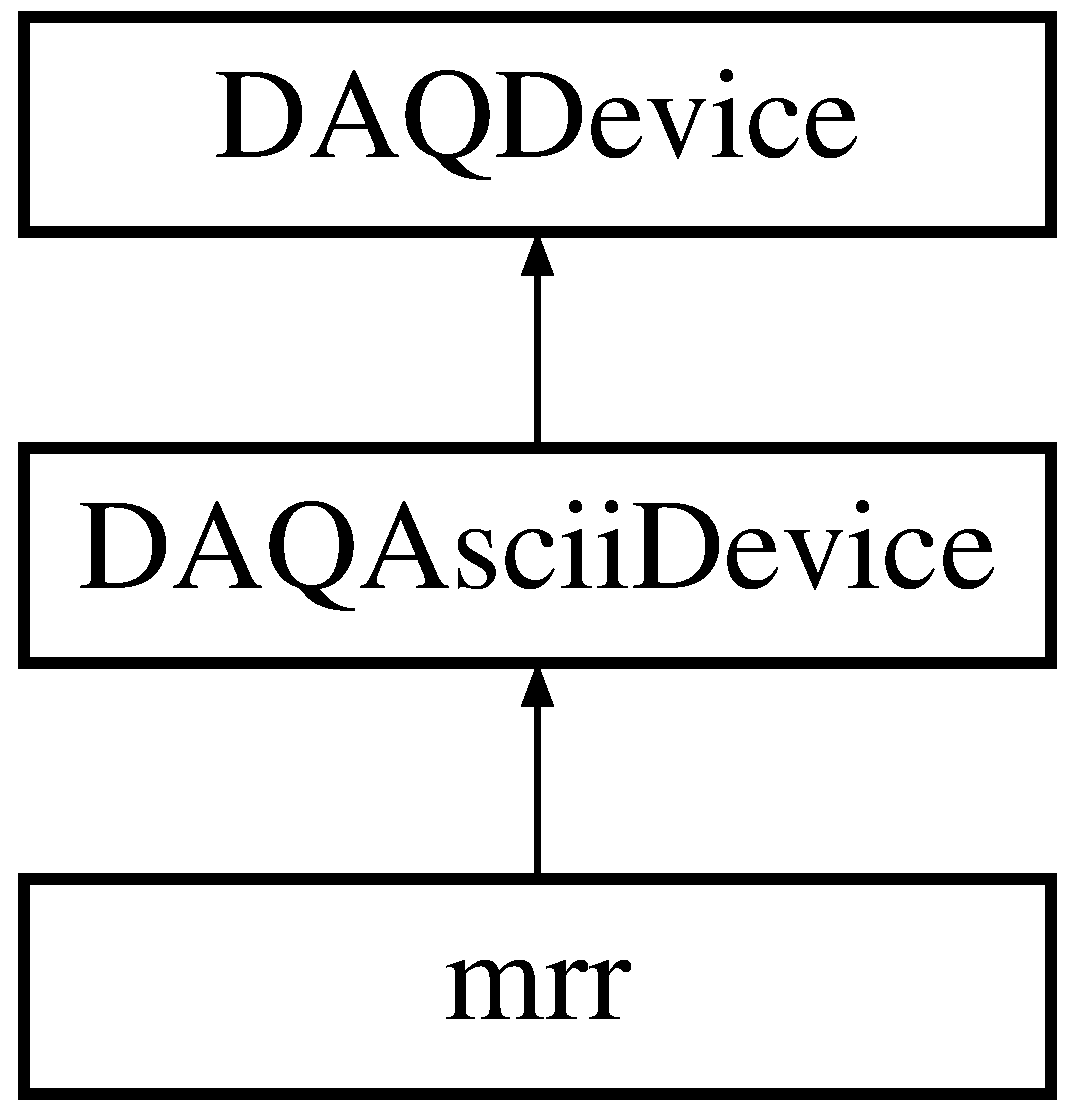
\includegraphics[height=3.000000cm]{classmrr}
\end{center}
\end{figure}
\subsection*{Public Member Functions}
\begin{DoxyCompactItemize}
\item 
\hyperlink{classmrr_a1a061ae8c23b5d12008f7b14c5eb1346}{mrr} ()
\item 
\hyperlink{classmrr_a2aaef911f158a4ad7922470d91378faf}{$\sim$mrr} ()
\item 
int \hyperlink{classmrr_a594cc3909052919f57881790f094b1fa}{read\-Header} (const char $\ast$\hyperlink{classDAQDevice_a7f9cda7cf5b41f6b134c313477e9644b}{filename})
\item 
void \hyperlink{classmrr_a36a73bcb154bafe4abed5c69c374e96f}{write\-Header} ()
\item 
void \hyperlink{classmrr_a781f21c62e91952f18fef385bcb1be6c}{write\-Data} ()
\item 
unsigned int \hyperlink{classmrr_a830a95365f1abeba05a339d5823cd6ac}{get\-Sensor\-Group} ()
\item 
void \hyperlink{classmrr_a748ac19e38528725bb1794cbd50a1748}{read\-Data} (std\-::string full\-\_\-filename)
\end{DoxyCompactItemize}
\subsection*{Additional Inherited Members}


\subsection{Detailed Description}
Implementation for the mrr device 

\subsection{Constructor \& Destructor Documentation}
\hypertarget{classmrr_a1a061ae8c23b5d12008f7b14c5eb1346}{\index{mrr@{mrr}!mrr@{mrr}}
\index{mrr@{mrr}!mrr@{mrr}}
\subsubsection[{mrr}]{\setlength{\rightskip}{0pt plus 5cm}mrr\-::mrr (
\begin{DoxyParamCaption}
{}
\end{DoxyParamCaption}
)}}\label{classmrr_a1a061ae8c23b5d12008f7b14c5eb1346}
\hypertarget{classmrr_a2aaef911f158a4ad7922470d91378faf}{\index{mrr@{mrr}!$\sim$mrr@{$\sim$mrr}}
\index{$\sim$mrr@{$\sim$mrr}!mrr@{mrr}}
\subsubsection[{$\sim$mrr}]{\setlength{\rightskip}{0pt plus 5cm}mrr\-::$\sim$mrr (
\begin{DoxyParamCaption}
{}
\end{DoxyParamCaption}
)}}\label{classmrr_a2aaef911f158a4ad7922470d91378faf}


\subsection{Member Function Documentation}
\hypertarget{classmrr_a830a95365f1abeba05a339d5823cd6ac}{\index{mrr@{mrr}!get\-Sensor\-Group@{get\-Sensor\-Group}}
\index{get\-Sensor\-Group@{get\-Sensor\-Group}!mrr@{mrr}}
\subsubsection[{get\-Sensor\-Group}]{\setlength{\rightskip}{0pt plus 5cm}unsigned int mrr\-::get\-Sensor\-Group (
\begin{DoxyParamCaption}
{}
\end{DoxyParamCaption}
)\hspace{0.3cm}{\ttfamily [virtual]}}}\label{classmrr_a830a95365f1abeba05a339d5823cd6ac}
Define a sensor group number for all the availble sensor group files 

Reimplemented from \hyperlink{classDAQDevice_a61d08492a11c30944dfaf3b86115abe8}{D\-A\-Q\-Device}.

\hypertarget{classmrr_a748ac19e38528725bb1794cbd50a1748}{\index{mrr@{mrr}!read\-Data@{read\-Data}}
\index{read\-Data@{read\-Data}!mrr@{mrr}}
\subsubsection[{read\-Data}]{\setlength{\rightskip}{0pt plus 5cm}void mrr\-::read\-Data (
\begin{DoxyParamCaption}
\item[{std\-::string}]{full\-\_\-filename}
\end{DoxyParamCaption}
)\hspace{0.3cm}{\ttfamily [virtual]}}}\label{classmrr_a748ac19e38528725bb1794cbd50a1748}


Reimplemented from \hyperlink{classDAQAsciiDevice_a0d9b17803680d966c7025ca6f174cef0}{D\-A\-Q\-Ascii\-Device}.

\hypertarget{classmrr_a594cc3909052919f57881790f094b1fa}{\index{mrr@{mrr}!read\-Header@{read\-Header}}
\index{read\-Header@{read\-Header}!mrr@{mrr}}
\subsubsection[{read\-Header}]{\setlength{\rightskip}{0pt plus 5cm}int mrr\-::read\-Header (
\begin{DoxyParamCaption}
\item[{const char $\ast$}]{header}
\end{DoxyParamCaption}
)\hspace{0.3cm}{\ttfamily [virtual]}}}\label{classmrr_a594cc3909052919f57881790f094b1fa}
Get time until next sample and it's id 

Reimplemented from \hyperlink{classDAQAsciiDevice_a5fce725c52b70ef2f56a34b32a03e15d}{D\-A\-Q\-Ascii\-Device}.

\hypertarget{classmrr_a781f21c62e91952f18fef385bcb1be6c}{\index{mrr@{mrr}!write\-Data@{write\-Data}}
\index{write\-Data@{write\-Data}!mrr@{mrr}}
\subsubsection[{write\-Data}]{\setlength{\rightskip}{0pt plus 5cm}void mrr\-::write\-Data (
\begin{DoxyParamCaption}
{}
\end{DoxyParamCaption}
)\hspace{0.3cm}{\ttfamily [virtual]}}}\label{classmrr_a781f21c62e91952f18fef385bcb1be6c}


Reimplemented from \hyperlink{classDAQDevice_acdc9d3765b1dfd845f99ec9c93071811}{D\-A\-Q\-Device}.

\hypertarget{classmrr_a36a73bcb154bafe4abed5c69c374e96f}{\index{mrr@{mrr}!write\-Header@{write\-Header}}
\index{write\-Header@{write\-Header}!mrr@{mrr}}
\subsubsection[{write\-Header}]{\setlength{\rightskip}{0pt plus 5cm}void mrr\-::write\-Header (
\begin{DoxyParamCaption}
{}
\end{DoxyParamCaption}
)\hspace{0.3cm}{\ttfamily [virtual]}}}\label{classmrr_a36a73bcb154bafe4abed5c69c374e96f}


Reimplemented from \hyperlink{classDAQDevice_aad39c13f039abd6e6a9b0aa21a7c8a4d}{D\-A\-Q\-Device}.



The documentation for this class was generated from the following files\-:\begin{DoxyCompactItemize}
\item 
/home/ntj/\-Development/phd/kitcube-\/tools/src/kitcube-\/devices/\hyperlink{mrr_8h}{mrr.\-h}\item 
/home/ntj/\-Development/phd/kitcube-\/tools/src/kitcube-\/devices/\hyperlink{mrr_8cpp}{mrr.\-cpp}\end{DoxyCompactItemize}

\hypertarget{classNorbert}{\section{Norbert Class Reference}
\label{classNorbert}\index{Norbert@{Norbert}}
}


{\ttfamily \#include $<$norbert.\-h$>$}

Inheritance diagram for Norbert\-:\begin{figure}[H]
\begin{center}
\leavevmode
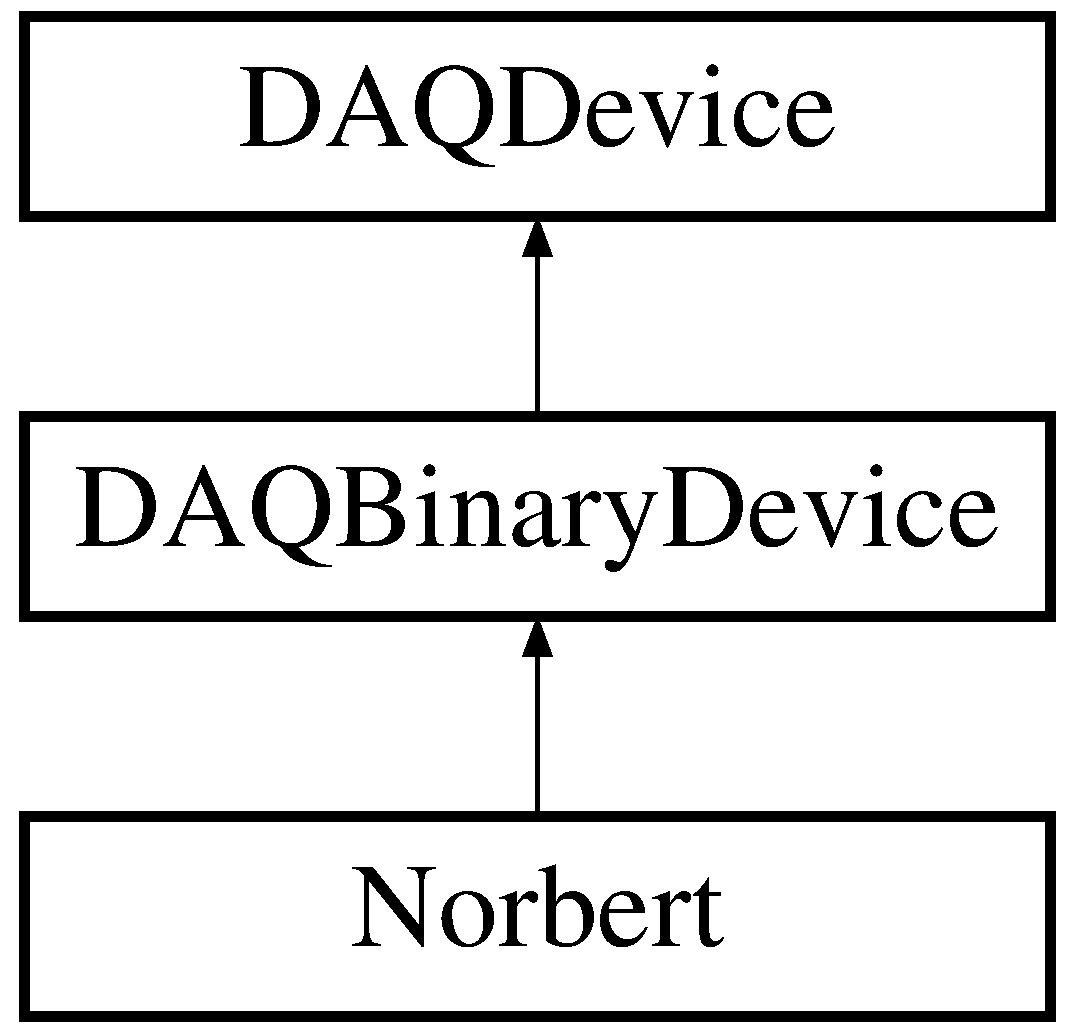
\includegraphics[height=3.000000cm]{classNorbert}
\end{center}
\end{figure}
\subsection*{Public Member Functions}
\begin{DoxyCompactItemize}
\item 
\hyperlink{classNorbert_a113d6cad08c22aafd3e63ccee4841f90}{Norbert} ()
\item 
\hyperlink{classNorbert_a27bd1709c30873d5438653789c6a6c6e}{$\sim$\-Norbert} ()
\item 
void \hyperlink{classNorbert_a3144651319dd271f84757d1ea1669ba1}{set\-Config\-Defaults} ()
\item 
const char $\ast$ \hyperlink{classNorbert_a8b111e6c53af877a765b9c9938a841b9}{get\-Data\-Dir} ()
\item 
void \hyperlink{classNorbert_a6a794ac4b3102bc7d857518c2c09ceff}{replace\-Item} (const char $\ast$$\ast$header, const char $\ast$item\-Tag, const char $\ast$new\-Value)
\item 
const char $\ast$ \hyperlink{classNorbert_a9445ec735a568ebd487ae750e709eae7}{get\-String\-Item} (const char $\ast$$\ast$header, const char $\ast$item\-Tag)
\item 
int \hyperlink{classNorbert_a10bcb21bf14fc71f916edd8ff0583c73}{get\-Numeric\-Item} (const char $\ast$$\ast$header, const char $\ast$item\-Tag)
\item 
unsigned int \hyperlink{classNorbert_a87b849c0c5fa73636de5e413f17033b7}{get\-Sensor\-Group} ()
\item 
long \hyperlink{classNorbert_a1f346f31e3c69c956a3a177ca13fed91}{get\-File\-Number} (char $\ast$\hyperlink{classDAQDevice_a7f9cda7cf5b41f6b134c313477e9644b}{filename})
\item 
int \hyperlink{classNorbert_a522857eace03f70822689acf6ad0e6eb}{read\-Header} (const char $\ast$header)
\item 
void \hyperlink{classNorbert_a0f0cf702bcacd76ab4d68d0334443bbe}{write\-Header} ()
\item 
void \hyperlink{classNorbert_a0b1b1ba6fc63b8662a537c66815ff19b}{read\-Data} (std\-::string full\-\_\-filename)
\item 
void \hyperlink{classNorbert_a2187d668d3c73ad112c223b82460064b}{update\-Data\-Set} (unsigned char $\ast$buf)
\end{DoxyCompactItemize}
\subsection*{Private Attributes}
\begin{DoxyCompactItemize}
\item 
unsigned char $\ast$ \hyperlink{classNorbert_a6f35c603a911f44e8d436bfa3ee3d166}{header\-Raw}
\item 
std\-::string \hyperlink{classNorbert_a7970cd046899ac6ae80af302650ac0de}{experiment\-Name}
\item 
unsigned long \hyperlink{classNorbert_ad046d88d69a2c5e0eb93e7f1b26bc5fd}{t\-Sample}
\item 
struct timeval \hyperlink{classNorbert_ac6365eaac8871d1af382adf9700b3e82}{t\-Ref}
\end{DoxyCompactItemize}
\subsection*{Additional Inherited Members}


\subsection{Detailed Description}
Implementation for the norbert simulation device. 

\subsection{Constructor \& Destructor Documentation}
\hypertarget{classNorbert_a113d6cad08c22aafd3e63ccee4841f90}{\index{Norbert@{Norbert}!Norbert@{Norbert}}
\index{Norbert@{Norbert}!Norbert@{Norbert}}
\subsubsection[{Norbert}]{\setlength{\rightskip}{0pt plus 5cm}Norbert\-::\-Norbert (
\begin{DoxyParamCaption}
{}
\end{DoxyParamCaption}
)}}\label{classNorbert_a113d6cad08c22aafd3e63ccee4841f90}
Constructor \hypertarget{classNorbert_a27bd1709c30873d5438653789c6a6c6e}{\index{Norbert@{Norbert}!$\sim$\-Norbert@{$\sim$\-Norbert}}
\index{$\sim$\-Norbert@{$\sim$\-Norbert}!Norbert@{Norbert}}
\subsubsection[{$\sim$\-Norbert}]{\setlength{\rightskip}{0pt plus 5cm}Norbert\-::$\sim$\-Norbert (
\begin{DoxyParamCaption}
{}
\end{DoxyParamCaption}
)}}\label{classNorbert_a27bd1709c30873d5438653789c6a6c6e}
Destructor 

\subsection{Member Function Documentation}
\hypertarget{classNorbert_a8b111e6c53af877a765b9c9938a841b9}{\index{Norbert@{Norbert}!get\-Data\-Dir@{get\-Data\-Dir}}
\index{get\-Data\-Dir@{get\-Data\-Dir}!Norbert@{Norbert}}
\subsubsection[{get\-Data\-Dir}]{\setlength{\rightskip}{0pt plus 5cm}const char $\ast$ Norbert\-::get\-Data\-Dir (
\begin{DoxyParamCaption}
{}
\end{DoxyParamCaption}
)\hspace{0.3cm}{\ttfamily [virtual]}}}\label{classNorbert_a8b111e6c53af877a765b9c9938a841b9}
Read parameter from inifile Returns the path relative to the base path to the data dir 

Reimplemented from \hyperlink{classDAQDevice_a7d7d41f0c1496221e589d84b38d1c865}{D\-A\-Q\-Device}.

\hypertarget{classNorbert_a1f346f31e3c69c956a3a177ca13fed91}{\index{Norbert@{Norbert}!get\-File\-Number@{get\-File\-Number}}
\index{get\-File\-Number@{get\-File\-Number}!Norbert@{Norbert}}
\subsubsection[{get\-File\-Number}]{\setlength{\rightskip}{0pt plus 5cm}long Norbert\-::get\-File\-Number (
\begin{DoxyParamCaption}
\item[{char $\ast$}]{filename}
\end{DoxyParamCaption}
)\hspace{0.3cm}{\ttfamily [virtual]}}}\label{classNorbert_a1f346f31e3c69c956a3a177ca13fed91}
Re-\/implement the calculation of the file numbering scheme. The ceilometer uses date and times in the filename 

Reimplemented from \hyperlink{classDAQDevice_a56a712062b2b17c6a73cb7fb0a475d2e}{D\-A\-Q\-Device}.

\hypertarget{classNorbert_a10bcb21bf14fc71f916edd8ff0583c73}{\index{Norbert@{Norbert}!get\-Numeric\-Item@{get\-Numeric\-Item}}
\index{get\-Numeric\-Item@{get\-Numeric\-Item}!Norbert@{Norbert}}
\subsubsection[{get\-Numeric\-Item}]{\setlength{\rightskip}{0pt plus 5cm}int Norbert\-::get\-Numeric\-Item (
\begin{DoxyParamCaption}
\item[{const char $\ast$$\ast$}]{header, }
\item[{const char $\ast$}]{item\-Tag}
\end{DoxyParamCaption}
)}}\label{classNorbert_a10bcb21bf14fc71f916edd8ff0583c73}
\hypertarget{classNorbert_a87b849c0c5fa73636de5e413f17033b7}{\index{Norbert@{Norbert}!get\-Sensor\-Group@{get\-Sensor\-Group}}
\index{get\-Sensor\-Group@{get\-Sensor\-Group}!Norbert@{Norbert}}
\subsubsection[{get\-Sensor\-Group}]{\setlength{\rightskip}{0pt plus 5cm}unsigned int Norbert\-::get\-Sensor\-Group (
\begin{DoxyParamCaption}
{}
\end{DoxyParamCaption}
)\hspace{0.3cm}{\ttfamily [virtual]}}}\label{classNorbert_a87b849c0c5fa73636de5e413f17033b7}
Define a sensor group number for all the availble sensor group files 

Reimplemented from \hyperlink{classDAQDevice_a61d08492a11c30944dfaf3b86115abe8}{D\-A\-Q\-Device}.

\hypertarget{classNorbert_a9445ec735a568ebd487ae750e709eae7}{\index{Norbert@{Norbert}!get\-String\-Item@{get\-String\-Item}}
\index{get\-String\-Item@{get\-String\-Item}!Norbert@{Norbert}}
\subsubsection[{get\-String\-Item}]{\setlength{\rightskip}{0pt plus 5cm}const char $\ast$ Norbert\-::get\-String\-Item (
\begin{DoxyParamCaption}
\item[{const char $\ast$$\ast$}]{header, }
\item[{const char $\ast$}]{item\-Tag}
\end{DoxyParamCaption}
)}}\label{classNorbert_a9445ec735a568ebd487ae750e709eae7}
\hypertarget{classNorbert_a0b1b1ba6fc63b8662a537c66815ff19b}{\index{Norbert@{Norbert}!read\-Data@{read\-Data}}
\index{read\-Data@{read\-Data}!Norbert@{Norbert}}
\subsubsection[{read\-Data}]{\setlength{\rightskip}{0pt plus 5cm}void Norbert\-::read\-Data (
\begin{DoxyParamCaption}
\item[{std\-::string}]{full\-\_\-filename}
\end{DoxyParamCaption}
)\hspace{0.3cm}{\ttfamily [virtual]}}}\label{classNorbert_a0b1b1ba6fc63b8662a537c66815ff19b}


Reimplemented from \hyperlink{classDAQBinaryDevice_a725281822b7945b8c1154d079c0011ff}{D\-A\-Q\-Binary\-Device}.

\hypertarget{classNorbert_a522857eace03f70822689acf6ad0e6eb}{\index{Norbert@{Norbert}!read\-Header@{read\-Header}}
\index{read\-Header@{read\-Header}!Norbert@{Norbert}}
\subsubsection[{read\-Header}]{\setlength{\rightskip}{0pt plus 5cm}int Norbert\-::read\-Header (
\begin{DoxyParamCaption}
\item[{const char $\ast$}]{header}
\end{DoxyParamCaption}
)\hspace{0.3cm}{\ttfamily [virtual]}}}\label{classNorbert_a522857eace03f70822689acf6ad0e6eb}
Get time until next sample and it's id 

Reimplemented from \hyperlink{classDAQDevice_af5fa373af9a089c18c7fd1d662db144f}{D\-A\-Q\-Device}.

\hypertarget{classNorbert_a6a794ac4b3102bc7d857518c2c09ceff}{\index{Norbert@{Norbert}!replace\-Item@{replace\-Item}}
\index{replace\-Item@{replace\-Item}!Norbert@{Norbert}}
\subsubsection[{replace\-Item}]{\setlength{\rightskip}{0pt plus 5cm}void Norbert\-::replace\-Item (
\begin{DoxyParamCaption}
\item[{const char $\ast$$\ast$}]{header, }
\item[{const char $\ast$}]{item\-Tag, }
\item[{const char $\ast$}]{new\-Value}
\end{DoxyParamCaption}
)}}\label{classNorbert_a6a794ac4b3102bc7d857518c2c09ceff}
\hypertarget{classNorbert_a3144651319dd271f84757d1ea1669ba1}{\index{Norbert@{Norbert}!set\-Config\-Defaults@{set\-Config\-Defaults}}
\index{set\-Config\-Defaults@{set\-Config\-Defaults}!Norbert@{Norbert}}
\subsubsection[{set\-Config\-Defaults}]{\setlength{\rightskip}{0pt plus 5cm}void Norbert\-::set\-Config\-Defaults (
\begin{DoxyParamCaption}
{}
\end{DoxyParamCaption}
)\hspace{0.3cm}{\ttfamily [virtual]}}}\label{classNorbert_a3144651319dd271f84757d1ea1669ba1}
Set default configuration 

Reimplemented from \hyperlink{classDAQDevice_a7685cec80865752cc0ef3ab49c6c2277}{D\-A\-Q\-Device}.

\hypertarget{classNorbert_a2187d668d3c73ad112c223b82460064b}{\index{Norbert@{Norbert}!update\-Data\-Set@{update\-Data\-Set}}
\index{update\-Data\-Set@{update\-Data\-Set}!Norbert@{Norbert}}
\subsubsection[{update\-Data\-Set}]{\setlength{\rightskip}{0pt plus 5cm}void Norbert\-::update\-Data\-Set (
\begin{DoxyParamCaption}
\item[{unsigned char $\ast$}]{buf}
\end{DoxyParamCaption}
)\hspace{0.3cm}{\ttfamily [virtual]}}}\label{classNorbert_a2187d668d3c73ad112c223b82460064b}
Replace time stamp in the data set by the current time 

Reimplemented from \hyperlink{classDAQDevice_a06d18d7b372d35c55f8a1a399f582a94}{D\-A\-Q\-Device}.

\hypertarget{classNorbert_a0f0cf702bcacd76ab4d68d0334443bbe}{\index{Norbert@{Norbert}!write\-Header@{write\-Header}}
\index{write\-Header@{write\-Header}!Norbert@{Norbert}}
\subsubsection[{write\-Header}]{\setlength{\rightskip}{0pt plus 5cm}void Norbert\-::write\-Header (
\begin{DoxyParamCaption}
{}
\end{DoxyParamCaption}
)\hspace{0.3cm}{\ttfamily [virtual]}}}\label{classNorbert_a0f0cf702bcacd76ab4d68d0334443bbe}


Reimplemented from \hyperlink{classDAQDevice_aad39c13f039abd6e6a9b0aa21a7c8a4d}{D\-A\-Q\-Device}.



\subsection{Member Data Documentation}
\hypertarget{classNorbert_a7970cd046899ac6ae80af302650ac0de}{\index{Norbert@{Norbert}!experiment\-Name@{experiment\-Name}}
\index{experiment\-Name@{experiment\-Name}!Norbert@{Norbert}}
\subsubsection[{experiment\-Name}]{\setlength{\rightskip}{0pt plus 5cm}std\-::string Norbert\-::experiment\-Name\hspace{0.3cm}{\ttfamily [private]}}}\label{classNorbert_a7970cd046899ac6ae80af302650ac0de}
\hypertarget{classNorbert_a6f35c603a911f44e8d436bfa3ee3d166}{\index{Norbert@{Norbert}!header\-Raw@{header\-Raw}}
\index{header\-Raw@{header\-Raw}!Norbert@{Norbert}}
\subsubsection[{header\-Raw}]{\setlength{\rightskip}{0pt plus 5cm}unsigned char$\ast$ Norbert\-::header\-Raw\hspace{0.3cm}{\ttfamily [private]}}}\label{classNorbert_a6f35c603a911f44e8d436bfa3ee3d166}
\hypertarget{classNorbert_ac6365eaac8871d1af382adf9700b3e82}{\index{Norbert@{Norbert}!t\-Ref@{t\-Ref}}
\index{t\-Ref@{t\-Ref}!Norbert@{Norbert}}
\subsubsection[{t\-Ref}]{\setlength{\rightskip}{0pt plus 5cm}struct timeval Norbert\-::t\-Ref\hspace{0.3cm}{\ttfamily [private]}}}\label{classNorbert_ac6365eaac8871d1af382adf9700b3e82}
\hypertarget{classNorbert_ad046d88d69a2c5e0eb93e7f1b26bc5fd}{\index{Norbert@{Norbert}!t\-Sample@{t\-Sample}}
\index{t\-Sample@{t\-Sample}!Norbert@{Norbert}}
\subsubsection[{t\-Sample}]{\setlength{\rightskip}{0pt plus 5cm}unsigned long Norbert\-::t\-Sample\hspace{0.3cm}{\ttfamily [private]}}}\label{classNorbert_ad046d88d69a2c5e0eb93e7f1b26bc5fd}


The documentation for this class was generated from the following files\-:\begin{DoxyCompactItemize}
\item 
/home/ntj/\-Development/phd/kitcube-\/tools/src/kitcube-\/devices/\hyperlink{norbert_8h}{norbert.\-h}\item 
/home/ntj/\-Development/phd/kitcube-\/tools/src/kitcube-\/devices/\hyperlink{norbert_8cpp}{norbert.\-cpp}\end{DoxyCompactItemize}

\hypertarget{classOrcaProcess}{\section{Orca\-Process Class Reference}
\label{classOrcaProcess}\index{Orca\-Process@{Orca\-Process}}
}


{\ttfamily \#include $<$orcaprocess.\-h$>$}

Inheritance diagram for Orca\-Process\-:\begin{figure}[H]
\begin{center}
\leavevmode
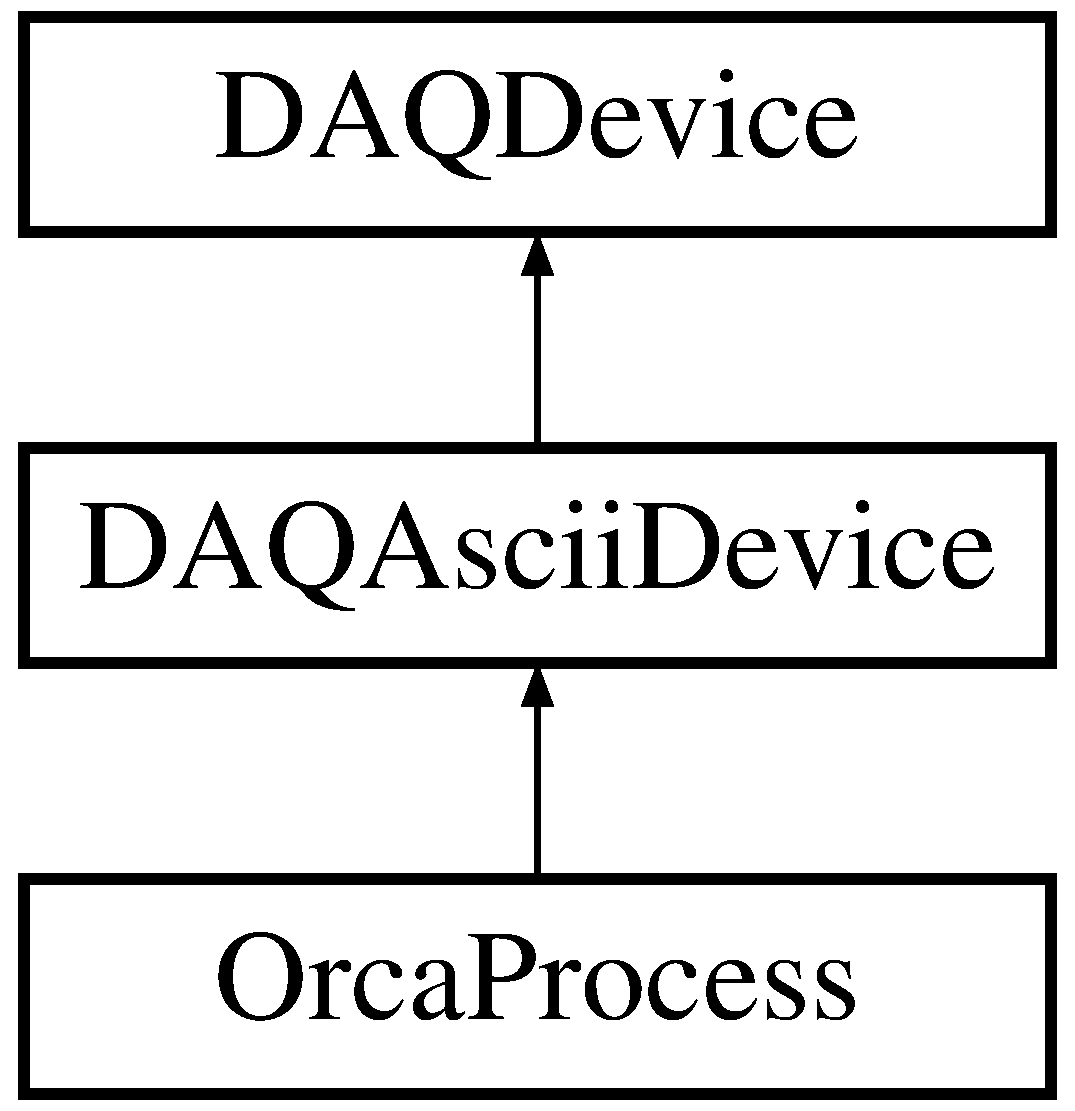
\includegraphics[height=3.000000cm]{classOrcaProcess}
\end{center}
\end{figure}
\subsection*{Public Member Functions}
\begin{DoxyCompactItemize}
\item 
\hyperlink{classOrcaProcess_add7cf4d095b94f701662b4fc051d1600}{Orca\-Process} ()
\item 
\hyperlink{classOrcaProcess_aca7bc651902e89fcb147745eeb57c671}{$\sim$\-Orca\-Process} ()
\item 
void \hyperlink{classOrcaProcess_a987ff32d0ec211530e76e108bd5e0460}{set\-Config\-Defaults} ()
\item 
int \hyperlink{classOrcaProcess_af433a05b744459be6427500d237c23c8}{read\-Header} (const char $\ast$\hyperlink{classDAQDevice_a7f9cda7cf5b41f6b134c313477e9644b}{filename})
\item 
int \hyperlink{classOrcaProcess_a3bfc4800f22f99f2370cd513a4a19c7c}{parse\-Data} (char $\ast$line, struct timeval $\ast$l\-\_\-t\-Data, double $\ast$\hyperlink{classDAQDevice_ad148188c57598fdf4fd4c1c333aeb0d8}{sensor\-Value})
\item 
unsigned int \hyperlink{classOrcaProcess_ab22bbbebedbbedeb83965377fb2b302b}{get\-Sensor\-Group} ()
\end{DoxyCompactItemize}
\subsection*{Private Attributes}
\begin{DoxyCompactItemize}
\item 
struct timeval \hyperlink{classOrcaProcess_a1102459cdbab05a4bb25475c12acbc12}{start\-\_\-time}
\item 
int \hyperlink{classOrcaProcess_a2d931dc79514b21a612a531bfb4190fa}{n\-Map}
\item 
int \hyperlink{classOrcaProcess_aac55db93ffac32ffa0b5bf1cf0975ac6}{map} \mbox{[}32\mbox{]}
\end{DoxyCompactItemize}
\subsection*{Additional Inherited Members}


\subsection{Constructor \& Destructor Documentation}
\hypertarget{classOrcaProcess_add7cf4d095b94f701662b4fc051d1600}{\index{Orca\-Process@{Orca\-Process}!Orca\-Process@{Orca\-Process}}
\index{Orca\-Process@{Orca\-Process}!OrcaProcess@{Orca\-Process}}
\subsubsection[{Orca\-Process}]{\setlength{\rightskip}{0pt plus 5cm}Orca\-Process\-::\-Orca\-Process (
\begin{DoxyParamCaption}
{}
\end{DoxyParamCaption}
)}}\label{classOrcaProcess_add7cf4d095b94f701662b4fc051d1600}
\hypertarget{classOrcaProcess_aca7bc651902e89fcb147745eeb57c671}{\index{Orca\-Process@{Orca\-Process}!$\sim$\-Orca\-Process@{$\sim$\-Orca\-Process}}
\index{$\sim$\-Orca\-Process@{$\sim$\-Orca\-Process}!OrcaProcess@{Orca\-Process}}
\subsubsection[{$\sim$\-Orca\-Process}]{\setlength{\rightskip}{0pt plus 5cm}Orca\-Process\-::$\sim$\-Orca\-Process (
\begin{DoxyParamCaption}
{}
\end{DoxyParamCaption}
)}}\label{classOrcaProcess_aca7bc651902e89fcb147745eeb57c671}


\subsection{Member Function Documentation}
\hypertarget{classOrcaProcess_ab22bbbebedbbedeb83965377fb2b302b}{\index{Orca\-Process@{Orca\-Process}!get\-Sensor\-Group@{get\-Sensor\-Group}}
\index{get\-Sensor\-Group@{get\-Sensor\-Group}!OrcaProcess@{Orca\-Process}}
\subsubsection[{get\-Sensor\-Group}]{\setlength{\rightskip}{0pt plus 5cm}unsigned int Orca\-Process\-::get\-Sensor\-Group (
\begin{DoxyParamCaption}
{}
\end{DoxyParamCaption}
)\hspace{0.3cm}{\ttfamily [virtual]}}}\label{classOrcaProcess_ab22bbbebedbbedeb83965377fb2b302b}
Define a sensor group number for all the availble sensor group files 

Reimplemented from \hyperlink{classDAQDevice_a61d08492a11c30944dfaf3b86115abe8}{D\-A\-Q\-Device}.

\hypertarget{classOrcaProcess_a3bfc4800f22f99f2370cd513a4a19c7c}{\index{Orca\-Process@{Orca\-Process}!parse\-Data@{parse\-Data}}
\index{parse\-Data@{parse\-Data}!OrcaProcess@{Orca\-Process}}
\subsubsection[{parse\-Data}]{\setlength{\rightskip}{0pt plus 5cm}int Orca\-Process\-::parse\-Data (
\begin{DoxyParamCaption}
\item[{char $\ast$}]{line, }
\item[{struct timeval $\ast$}]{l\-\_\-t\-Data, }
\item[{double $\ast$}]{sensor\-Value}
\end{DoxyParamCaption}
)\hspace{0.3cm}{\ttfamily [virtual]}}}\label{classOrcaProcess_a3bfc4800f22f99f2370cd513a4a19c7c}
Read the data from the current line of the data file. \begin{DoxyReturn}{Returns}
-\/1 no data found, skip storage 0 sucess, store data, 1 read another line 
\end{DoxyReturn}


Reimplemented from \hyperlink{classDAQAsciiDevice_a9c20d9d69af4ba1641dbc82dd5be2aa5}{D\-A\-Q\-Ascii\-Device}.

\hypertarget{classOrcaProcess_af433a05b744459be6427500d237c23c8}{\index{Orca\-Process@{Orca\-Process}!read\-Header@{read\-Header}}
\index{read\-Header@{read\-Header}!OrcaProcess@{Orca\-Process}}
\subsubsection[{read\-Header}]{\setlength{\rightskip}{0pt plus 5cm}int Orca\-Process\-::read\-Header (
\begin{DoxyParamCaption}
\item[{const char $\ast$}]{header}
\end{DoxyParamCaption}
)\hspace{0.3cm}{\ttfamily [virtual]}}}\label{classOrcaProcess_af433a05b744459be6427500d237c23c8}
Get time until next sample and it's id 

Reimplemented from \hyperlink{classDAQAsciiDevice_a5fce725c52b70ef2f56a34b32a03e15d}{D\-A\-Q\-Ascii\-Device}.

\hypertarget{classOrcaProcess_a987ff32d0ec211530e76e108bd5e0460}{\index{Orca\-Process@{Orca\-Process}!set\-Config\-Defaults@{set\-Config\-Defaults}}
\index{set\-Config\-Defaults@{set\-Config\-Defaults}!OrcaProcess@{Orca\-Process}}
\subsubsection[{set\-Config\-Defaults}]{\setlength{\rightskip}{0pt plus 5cm}void Orca\-Process\-::set\-Config\-Defaults (
\begin{DoxyParamCaption}
{}
\end{DoxyParamCaption}
)\hspace{0.3cm}{\ttfamily [virtual]}}}\label{classOrcaProcess_a987ff32d0ec211530e76e108bd5e0460}
The function is called before reading the configuration from the inifile. Use this fucntion in the module specific implementation to override the standard defaults 

Reimplemented from \hyperlink{classDAQDevice_a7685cec80865752cc0ef3ab49c6c2277}{D\-A\-Q\-Device}.



\subsection{Member Data Documentation}
\hypertarget{classOrcaProcess_aac55db93ffac32ffa0b5bf1cf0975ac6}{\index{Orca\-Process@{Orca\-Process}!map@{map}}
\index{map@{map}!OrcaProcess@{Orca\-Process}}
\subsubsection[{map}]{\setlength{\rightskip}{0pt plus 5cm}int Orca\-Process\-::map\mbox{[}32\mbox{]}\hspace{0.3cm}{\ttfamily [private]}}}\label{classOrcaProcess_aac55db93ffac32ffa0b5bf1cf0975ac6}
Mapping of the sensors \hypertarget{classOrcaProcess_a2d931dc79514b21a612a531bfb4190fa}{\index{Orca\-Process@{Orca\-Process}!n\-Map@{n\-Map}}
\index{n\-Map@{n\-Map}!OrcaProcess@{Orca\-Process}}
\subsubsection[{n\-Map}]{\setlength{\rightskip}{0pt plus 5cm}int Orca\-Process\-::n\-Map\hspace{0.3cm}{\ttfamily [private]}}}\label{classOrcaProcess_a2d931dc79514b21a612a531bfb4190fa}
Number of channels in the P\-A\-C data files \hypertarget{classOrcaProcess_a1102459cdbab05a4bb25475c12acbc12}{\index{Orca\-Process@{Orca\-Process}!start\-\_\-time@{start\-\_\-time}}
\index{start\-\_\-time@{start\-\_\-time}!OrcaProcess@{Orca\-Process}}
\subsubsection[{start\-\_\-time}]{\setlength{\rightskip}{0pt plus 5cm}struct timeval Orca\-Process\-::start\-\_\-time\hspace{0.3cm}{\ttfamily [private]}}}\label{classOrcaProcess_a1102459cdbab05a4bb25475c12acbc12}


The documentation for this class was generated from the following files\-:\begin{DoxyCompactItemize}
\item 
/home/ntj/\-Development/phd/kitcube-\/tools/src/kitcube-\/devices/\hyperlink{orcaprocess_8h}{orcaprocess.\-h}\item 
/home/ntj/\-Development/phd/kitcube-\/tools/src/kitcube-\/devices/\hyperlink{orcaprocess_8cpp}{orcaprocess.\-cpp}\end{DoxyCompactItemize}

\hypertarget{classparsivel}{\section{parsivel Class Reference}
\label{classparsivel}\index{parsivel@{parsivel}}
}


{\ttfamily \#include $<$parsivel.\-h$>$}

Inheritance diagram for parsivel\-:\begin{figure}[H]
\begin{center}
\leavevmode
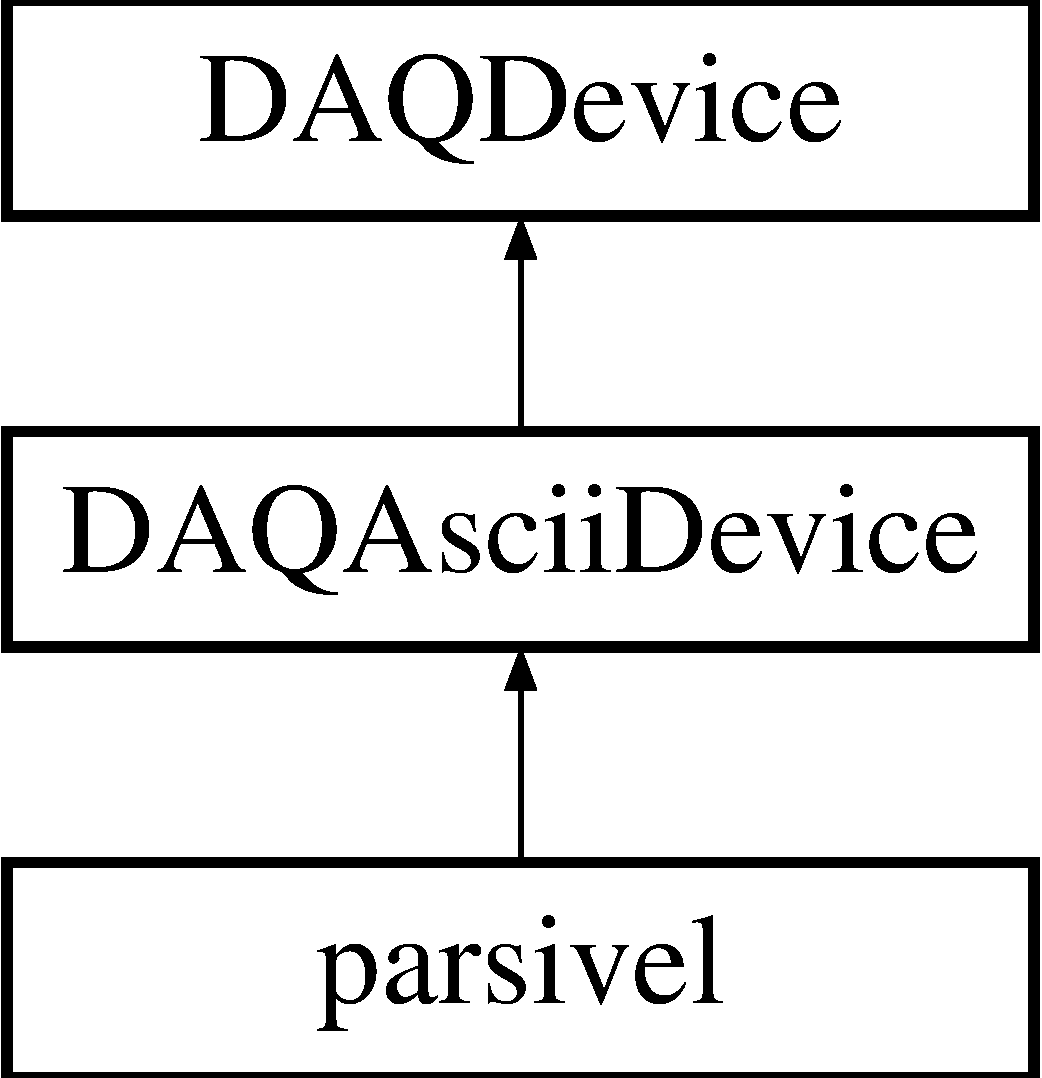
\includegraphics[height=3.000000cm]{classparsivel}
\end{center}
\end{figure}
\subsection*{Public Member Functions}
\begin{DoxyCompactItemize}
\item 
\hyperlink{classparsivel_a0744fdf7b0b79f498aa0ef3d9bcac0f2}{parsivel} ()
\item 
\hyperlink{classparsivel_a34d2688c5263aea7b7ac4c6e1f189c16}{$\sim$parsivel} ()
\item 
unsigned int \hyperlink{classparsivel_af756bf97da1b3023037090e9e7c1cfb8}{get\-Sensor\-Group} ()
\item 
int \hyperlink{classparsivel_ab2b3727aa63b91b2178d3ce5192ed830}{read\-Header} (const char $\ast$\hyperlink{classDAQDevice_a7f9cda7cf5b41f6b134c313477e9644b}{filename})
\item 
int \hyperlink{classparsivel_ab0195d09b023c63d725c551791c83462}{parse\-Data} (char $\ast$line, struct timeval $\ast$\hyperlink{classDAQDevice_af7da14a199a793fd63db3af2b2a78d92}{t\-Data}, double $\ast$\hyperlink{classDAQDevice_ad148188c57598fdf4fd4c1c333aeb0d8}{sensor\-Value})
\item 
void \hyperlink{classparsivel_a8e501c43f6ef4a197b92177729784286}{write\-Data} ()
\end{DoxyCompactItemize}
\subsection*{Additional Inherited Members}


\subsection{Detailed Description}
Implementation for the parsivel device.

The Parsivel measures the distribution of the rain drop size and speed. To save space in the database there is only the aggregated data stored and the profiles are skipped.

T\-O\-D\-O\-:
\begin{DoxyItemize}
\item Compress profile data. (Scalars should be uncompressed in order not to spoil the database performance) 
\end{DoxyItemize}

\subsection{Constructor \& Destructor Documentation}
\hypertarget{classparsivel_a0744fdf7b0b79f498aa0ef3d9bcac0f2}{\index{parsivel@{parsivel}!parsivel@{parsivel}}
\index{parsivel@{parsivel}!parsivel@{parsivel}}
\subsubsection[{parsivel}]{\setlength{\rightskip}{0pt plus 5cm}parsivel\-::parsivel (
\begin{DoxyParamCaption}
{}
\end{DoxyParamCaption}
)}}\label{classparsivel_a0744fdf7b0b79f498aa0ef3d9bcac0f2}
\hypertarget{classparsivel_a34d2688c5263aea7b7ac4c6e1f189c16}{\index{parsivel@{parsivel}!$\sim$parsivel@{$\sim$parsivel}}
\index{$\sim$parsivel@{$\sim$parsivel}!parsivel@{parsivel}}
\subsubsection[{$\sim$parsivel}]{\setlength{\rightskip}{0pt plus 5cm}parsivel\-::$\sim$parsivel (
\begin{DoxyParamCaption}
{}
\end{DoxyParamCaption}
)}}\label{classparsivel_a34d2688c5263aea7b7ac4c6e1f189c16}


\subsection{Member Function Documentation}
\hypertarget{classparsivel_af756bf97da1b3023037090e9e7c1cfb8}{\index{parsivel@{parsivel}!get\-Sensor\-Group@{get\-Sensor\-Group}}
\index{get\-Sensor\-Group@{get\-Sensor\-Group}!parsivel@{parsivel}}
\subsubsection[{get\-Sensor\-Group}]{\setlength{\rightskip}{0pt plus 5cm}unsigned int parsivel\-::get\-Sensor\-Group (
\begin{DoxyParamCaption}
{}
\end{DoxyParamCaption}
)\hspace{0.3cm}{\ttfamily [virtual]}}}\label{classparsivel_af756bf97da1b3023037090e9e7c1cfb8}
Define a sensor group number for all the availble sensor group files 

Reimplemented from \hyperlink{classDAQDevice_a61d08492a11c30944dfaf3b86115abe8}{D\-A\-Q\-Device}.

\hypertarget{classparsivel_ab0195d09b023c63d725c551791c83462}{\index{parsivel@{parsivel}!parse\-Data@{parse\-Data}}
\index{parse\-Data@{parse\-Data}!parsivel@{parsivel}}
\subsubsection[{parse\-Data}]{\setlength{\rightskip}{0pt plus 5cm}int parsivel\-::parse\-Data (
\begin{DoxyParamCaption}
\item[{char $\ast$}]{line, }
\item[{struct timeval $\ast$}]{t\-Data, }
\item[{double $\ast$}]{sensor\-Value}
\end{DoxyParamCaption}
)\hspace{0.3cm}{\ttfamily [virtual]}}}\label{classparsivel_ab0195d09b023c63d725c551791c83462}
The information of one dataset is split over five lines. The data is collected line by line. 

Reimplemented from \hyperlink{classDAQAsciiDevice_a9c20d9d69af4ba1641dbc82dd5be2aa5}{D\-A\-Q\-Ascii\-Device}.

\hypertarget{classparsivel_ab2b3727aa63b91b2178d3ce5192ed830}{\index{parsivel@{parsivel}!read\-Header@{read\-Header}}
\index{read\-Header@{read\-Header}!parsivel@{parsivel}}
\subsubsection[{read\-Header}]{\setlength{\rightskip}{0pt plus 5cm}int parsivel\-::read\-Header (
\begin{DoxyParamCaption}
\item[{const char $\ast$}]{filename}
\end{DoxyParamCaption}
)\hspace{0.3cm}{\ttfamily [virtual]}}}\label{classparsivel_ab2b3727aa63b91b2178d3ce5192ed830}
Defintion of the sensors 

Reimplemented from \hyperlink{classDAQAsciiDevice_a5fce725c52b70ef2f56a34b32a03e15d}{D\-A\-Q\-Ascii\-Device}.

\hypertarget{classparsivel_a8e501c43f6ef4a197b92177729784286}{\index{parsivel@{parsivel}!write\-Data@{write\-Data}}
\index{write\-Data@{write\-Data}!parsivel@{parsivel}}
\subsubsection[{write\-Data}]{\setlength{\rightskip}{0pt plus 5cm}void parsivel\-::write\-Data (
\begin{DoxyParamCaption}
{}
\end{DoxyParamCaption}
)\hspace{0.3cm}{\ttfamily [virtual]}}}\label{classparsivel_a8e501c43f6ef4a197b92177729784286}


Reimplemented from \hyperlink{classDAQDevice_acdc9d3765b1dfd845f99ec9c93071811}{D\-A\-Q\-Device}.



The documentation for this class was generated from the following files\-:\begin{DoxyCompactItemize}
\item 
/home/ntj/\-Development/phd/kitcube-\/tools/src/kitcube-\/devices/\hyperlink{parsivel_8h}{parsivel.\-h}\item 
/home/ntj/\-Development/phd/kitcube-\/tools/src/kitcube-\/devices/\hyperlink{parsivel_8cpp}{parsivel.\-cpp}\end{DoxyCompactItemize}

\hypertarget{classprocDuration}{\section{proc\-Duration Class Reference}
\label{classprocDuration}\index{proc\-Duration@{proc\-Duration}}
}


{\ttfamily \#include $<$proc\-Duration.\-h$>$}

\subsection*{Public Member Functions}
\begin{DoxyCompactItemize}
\item 
\hyperlink{classprocDuration_a350e96d176d438001311caa6b41391de}{proc\-Duration} ()
\item 
void \hyperlink{classprocDuration_aaad4302e83bbccc35b0906de8c0ab531}{set\-Start} ()
\item 
void \hyperlink{classprocDuration_ae0c09d3d0a81c78064e170ee02c38ee3}{set\-Start} (unsigned long time)
\item 
void \hyperlink{classprocDuration_a2baf0a30733d0045318d00ffc8020830}{set\-End} ()
\item 
void \hyperlink{classprocDuration_ae3c5853166d5c2983b1a508a3d783aae}{set\-End\-From\-Start} (\hyperlink{classprocDuration}{proc\-Duration} $\ast$dur)
\item 
double \hyperlink{classprocDuration_aca8f2bc01920b0bc85fcc8001b85854e}{get\-Duration\-C\-P\-U} ()
\item 
double \hyperlink{classprocDuration_a46a4097bb56d4d0694f3a9f39ff4047d}{get\-Duration\-R\-T} ()
\item 
void \hyperlink{classprocDuration_a31422e9f157639271e18d6fcc971418b}{display\-Duration} ()
\item 
void \hyperlink{classprocDuration_a2421fcd5372f2820f3d647b0b9ea7b5b}{display\-Duration} (F\-I\-L\-E $\ast$fout)
\item 
void \hyperlink{classprocDuration_a57e1c97ac11a00b4a752bfae1f13da51}{display\-Transfer\-Rate} (double blocksize)
\item 
void \hyperlink{classprocDuration_a6bc2cd76bfb9e29955c97a67d38767c9}{display\-Transfer\-Rate} (F\-I\-L\-E $\ast$fout, double blocksize)
\item 
void \hyperlink{classprocDuration_accfd22f8d3d3f564b933303cac3034d6}{display\-Start\-Time} (F\-I\-L\-E $\ast$fout)
\item 
void \hyperlink{classprocDuration_a683e15d56ba6c794fa24c2e23f2decb1}{display\-Start\-Date} (F\-I\-L\-E $\ast$fout)
\item 
const char $\ast$ \hyperlink{classprocDuration_ac005d66386a1dbb62e3d44dc06bab413}{c\-Start\-Time} ()
\item 
const char $\ast$ \hyperlink{classprocDuration_a1d0dab0ad00cd0adaec2beeb4754f2c1}{c\-Start\-Date} ()
\item 
const char $\ast$ \hyperlink{classprocDuration_aa6205795755ce1afdc3bc21dc96626e6}{c\-Start\-Zone} ()
\item 
const char $\ast$ \hyperlink{classprocDuration_a1aaa4d88d842e25ecbd3100c243796b6}{c\-End\-Time} ()
\item 
const char $\ast$ \hyperlink{classprocDuration_a45a2a3f05abad948d0a0e02e8e701ee3}{c\-End\-Date} ()
\item 
const char $\ast$ \hyperlink{classprocDuration_a28dc26f35d7e65394ee4758e2f9ab4c2}{c\-End\-Zone} ()
\item 
const char $\ast$ \hyperlink{classprocDuration_a1931042a18fac844d42cddf44101ef1e}{c\-Time} (time\-\_\-t $\ast$t)
\item 
const char $\ast$ \hyperlink{classprocDuration_a14c8907362b99a94d58f728ef024cd11}{c\-Gps\-Time} (unsigned long t)
\item 
const char $\ast$ \hyperlink{classprocDuration_a2b2ae30be812cb87c4dddeeefa9b78ad}{c\-Date} (time\-\_\-t $\ast$t)
\item 
const char $\ast$ \hyperlink{classprocDuration_a36b4b38f8275d9f5ecaf0a014d76f270}{c\-Gps\-Date} (unsigned long t)
\item 
const char $\ast$ \hyperlink{classprocDuration_afb0f7f2e14396c267acb338ba9ca597c}{c\-Zone} (time\-\_\-t $\ast$t)
\item 
unsigned long \hyperlink{classprocDuration_a760b8c8e6a76d51d22a8324920decadd}{get\-Start\-Sec} ()
\item 
unsigned long \hyperlink{classprocDuration_ae3358cdbb46bb778c4d0ccc000dab225}{get\-End\-Sec} ()
\item 
int \hyperlink{classprocDuration_ad15610a1b1998ef5d8923b041b3db153}{get\-Start\-Mili\-Sec} ()
\item 
int \hyperlink{classprocDuration_a66f7237d8ed5b63bd55964de89ebe5a6}{get\-End\-Mili\-Sec} ()
\item 
int \hyperlink{classprocDuration_ac1078f747a8c57360139962a6078fa2d}{get\-Start\-Micro\-Sec} ()
\item 
int \hyperlink{classprocDuration_abfb741c499aaa8e0a12f86ebb82df652}{get\-End\-Micro\-Sec} ()
\item 
int \hyperlink{classprocDuration_aff2364afd00b3c12e6143cf0dfb6980f}{get\-Start\-Nano\-Sec} ()
\item 
int \hyperlink{classprocDuration_a70a14db14b30e3b07af65554686e7d00}{get\-End\-Nano\-Sec} ()
\item 
void \hyperlink{classprocDuration_acf1c2d3c7fbc0cffa3513696c7f73c5a}{mean\-Time} (\hyperlink{classprocDuration}{proc\-Duration} \&dur)
\item 
void \hyperlink{classprocDuration_a4ada382bf6e2dbdca71fc941611fa5cd}{get\-Duration\-R\-T} (int $\ast$sign, unsigned long $\ast$sec, unsigned long $\ast$usec)
\item 
\hyperlink{classprocDuration}{proc\-Duration} \hyperlink{classprocDuration_a9da545dc00a5a8222b6731a62a44c3c5}{operator=} (\hyperlink{classprocDuration}{proc\-Duration} \&dur)
\item 
void \hyperlink{classprocDuration_a875e4c92cca07739eae35e0a7674c90f}{set} (\hyperlink{classprocDuration}{proc\-Duration} dur)
\end{DoxyCompactItemize}
\subsection*{Protected Attributes}
\begin{DoxyCompactItemize}
\item 
clock\-\_\-t \hyperlink{classprocDuration_a6305985898bc3c56d96bbbd315dce3d2}{start\-Tick}
\item 
clock\-\_\-t \hyperlink{classprocDuration_afb5dcb82095eed3ed2c16146c19cf448}{end\-Tick}
\item 
struct timeval \hyperlink{classprocDuration_a1f7a4f39023ba5f5786644e91f03ab7d}{start\-Time}
\item 
struct timezone \hyperlink{classprocDuration_a3a5ebfdf4aaaa8dacefefab93ef1ce40}{start\-Zone}
\item 
struct timeval \hyperlink{classprocDuration_aec55f4ad78f358669b7880083ac355a5}{end\-Time}
\item 
struct timezone \hyperlink{classprocDuration_a3f2c2451dc709af15bd6bf65b3308be4}{end\-Zone}
\item 
double \hyperlink{classprocDuration_a982ff57adecc307bf8daf6c3c5902414}{duration\-C\-P\-U}
\item 
double \hyperlink{classprocDuration_a1e3016ca8a92332b6f1427a9d008aeef}{duration\-R\-T}
\item 
int \hyperlink{classprocDuration_a72be56dcf2e5d2867b20e690f2796ef0}{diff\-Time\-Sign}
\item 
unsigned long \hyperlink{classprocDuration_ac9241af8f9ea5efa568e636683c22446}{diff\-Time\-Sec}
\item 
unsigned long \hyperlink{classprocDuration_a51854eb886bc5a872d2b930de46132e5}{diff\-Time\-Micro\-Sec}
\end{DoxyCompactItemize}
\subsection*{Static Protected Attributes}
\begin{DoxyCompactItemize}
\item 
static const char \hyperlink{classprocDuration_ae772881f1be51f9863b988e7fc7bfcf1}{dateformat} \mbox{[}$\,$\mbox{]} = \char`\"{}\%02d.\%02d.\%04d\char`\"{}
\item 
static const char \hyperlink{classprocDuration_a4f6bdff03e812b65c2c68e4d33f55d8c}{timeformat} \mbox{[}$\,$\mbox{]} = \char`\"{}\%02d\-:\%02d\-:\%02d\char`\"{}
\item 
static const char \hyperlink{classprocDuration_ac49a8c3058ed4ee10c2a61f03efafd96}{zoneformat} \mbox{[}$\,$\mbox{]} = \char`\"{}\%s\char`\"{}
\item 
static char \hyperlink{classprocDuration_acb961644d3635fca50247316e4888ff7}{datestring} \mbox{[}$\,$\mbox{]} = \char`\"{}dd.\-mm.\-jjjj\char`\"{}
\item 
static char \hyperlink{classprocDuration_ade868d17a31ee89d3453e8a32bf70c07}{timestring} \mbox{[}$\,$\mbox{]} = \char`\"{}hh\-:mm\-:ss\char`\"{}
\item 
static char \hyperlink{classprocDuration_a17e137b5abce3b50940a058c3b30f7e5}{zonestring} \mbox{[}$\,$\mbox{]} = \char`\"{} \char`\"{}
\end{DoxyCompactItemize}


\subsection{Detailed Description}
The class provide a timer like function to measure the real-\/time and the C\-P\-U time elapsed by a certain block of code. The time is used by setting start and stop point in the code. Afterwards the elapsed time can be displayed. 

\subsection{Constructor \& Destructor Documentation}
\hypertarget{classprocDuration_a350e96d176d438001311caa6b41391de}{\index{proc\-Duration@{proc\-Duration}!proc\-Duration@{proc\-Duration}}
\index{proc\-Duration@{proc\-Duration}!procDuration@{proc\-Duration}}
\subsubsection[{proc\-Duration}]{\setlength{\rightskip}{0pt plus 5cm}proc\-Duration\-::proc\-Duration (
\begin{DoxyParamCaption}
{}
\end{DoxyParamCaption}
)}}\label{classprocDuration_a350e96d176d438001311caa6b41391de}


\subsection{Member Function Documentation}
\hypertarget{classprocDuration_a2b2ae30be812cb87c4dddeeefa9b78ad}{\index{proc\-Duration@{proc\-Duration}!c\-Date@{c\-Date}}
\index{c\-Date@{c\-Date}!procDuration@{proc\-Duration}}
\subsubsection[{c\-Date}]{\setlength{\rightskip}{0pt plus 5cm}const char $\ast$ proc\-Duration\-::c\-Date (
\begin{DoxyParamCaption}
\item[{time\-\_\-t $\ast$}]{t}
\end{DoxyParamCaption}
)}}\label{classprocDuration_a2b2ae30be812cb87c4dddeeefa9b78ad}
Display the date of a given U\-T\-C time \hypertarget{classprocDuration_a45a2a3f05abad948d0a0e02e8e701ee3}{\index{proc\-Duration@{proc\-Duration}!c\-End\-Date@{c\-End\-Date}}
\index{c\-End\-Date@{c\-End\-Date}!procDuration@{proc\-Duration}}
\subsubsection[{c\-End\-Date}]{\setlength{\rightskip}{0pt plus 5cm}const char $\ast$ proc\-Duration\-::c\-End\-Date (
\begin{DoxyParamCaption}
{}
\end{DoxyParamCaption}
)}}\label{classprocDuration_a45a2a3f05abad948d0a0e02e8e701ee3}
Display the end date \hypertarget{classprocDuration_a1aaa4d88d842e25ecbd3100c243796b6}{\index{proc\-Duration@{proc\-Duration}!c\-End\-Time@{c\-End\-Time}}
\index{c\-End\-Time@{c\-End\-Time}!procDuration@{proc\-Duration}}
\subsubsection[{c\-End\-Time}]{\setlength{\rightskip}{0pt plus 5cm}const char $\ast$ proc\-Duration\-::c\-End\-Time (
\begin{DoxyParamCaption}
{}
\end{DoxyParamCaption}
)}}\label{classprocDuration_a1aaa4d88d842e25ecbd3100c243796b6}
Display the end time \hypertarget{classprocDuration_a28dc26f35d7e65394ee4758e2f9ab4c2}{\index{proc\-Duration@{proc\-Duration}!c\-End\-Zone@{c\-End\-Zone}}
\index{c\-End\-Zone@{c\-End\-Zone}!procDuration@{proc\-Duration}}
\subsubsection[{c\-End\-Zone}]{\setlength{\rightskip}{0pt plus 5cm}const char $\ast$ proc\-Duration\-::c\-End\-Zone (
\begin{DoxyParamCaption}
{}
\end{DoxyParamCaption}
)}}\label{classprocDuration_a28dc26f35d7e65394ee4758e2f9ab4c2}
Display the end timezone \hypertarget{classprocDuration_a36b4b38f8275d9f5ecaf0a014d76f270}{\index{proc\-Duration@{proc\-Duration}!c\-Gps\-Date@{c\-Gps\-Date}}
\index{c\-Gps\-Date@{c\-Gps\-Date}!procDuration@{proc\-Duration}}
\subsubsection[{c\-Gps\-Date}]{\setlength{\rightskip}{0pt plus 5cm}const char $\ast$ proc\-Duration\-::c\-Gps\-Date (
\begin{DoxyParamCaption}
\item[{unsigned long}]{t}
\end{DoxyParamCaption}
)}}\label{classprocDuration_a36b4b38f8275d9f5ecaf0a014d76f270}
Display the date of a given G\-P\-S time \hypertarget{classprocDuration_a14c8907362b99a94d58f728ef024cd11}{\index{proc\-Duration@{proc\-Duration}!c\-Gps\-Time@{c\-Gps\-Time}}
\index{c\-Gps\-Time@{c\-Gps\-Time}!procDuration@{proc\-Duration}}
\subsubsection[{c\-Gps\-Time}]{\setlength{\rightskip}{0pt plus 5cm}const char $\ast$ proc\-Duration\-::c\-Gps\-Time (
\begin{DoxyParamCaption}
\item[{unsigned long}]{t}
\end{DoxyParamCaption}
)}}\label{classprocDuration_a14c8907362b99a94d58f728ef024cd11}
Display the time of a given G\-P\-S time \hypertarget{classprocDuration_a1d0dab0ad00cd0adaec2beeb4754f2c1}{\index{proc\-Duration@{proc\-Duration}!c\-Start\-Date@{c\-Start\-Date}}
\index{c\-Start\-Date@{c\-Start\-Date}!procDuration@{proc\-Duration}}
\subsubsection[{c\-Start\-Date}]{\setlength{\rightskip}{0pt plus 5cm}const char $\ast$ proc\-Duration\-::c\-Start\-Date (
\begin{DoxyParamCaption}
{}
\end{DoxyParamCaption}
)}}\label{classprocDuration_a1d0dab0ad00cd0adaec2beeb4754f2c1}
Display the start date \hypertarget{classprocDuration_ac005d66386a1dbb62e3d44dc06bab413}{\index{proc\-Duration@{proc\-Duration}!c\-Start\-Time@{c\-Start\-Time}}
\index{c\-Start\-Time@{c\-Start\-Time}!procDuration@{proc\-Duration}}
\subsubsection[{c\-Start\-Time}]{\setlength{\rightskip}{0pt plus 5cm}const char $\ast$ proc\-Duration\-::c\-Start\-Time (
\begin{DoxyParamCaption}
{}
\end{DoxyParamCaption}
)}}\label{classprocDuration_ac005d66386a1dbb62e3d44dc06bab413}
Display the start time \hypertarget{classprocDuration_aa6205795755ce1afdc3bc21dc96626e6}{\index{proc\-Duration@{proc\-Duration}!c\-Start\-Zone@{c\-Start\-Zone}}
\index{c\-Start\-Zone@{c\-Start\-Zone}!procDuration@{proc\-Duration}}
\subsubsection[{c\-Start\-Zone}]{\setlength{\rightskip}{0pt plus 5cm}const char $\ast$ proc\-Duration\-::c\-Start\-Zone (
\begin{DoxyParamCaption}
{}
\end{DoxyParamCaption}
)}}\label{classprocDuration_aa6205795755ce1afdc3bc21dc96626e6}
Display the start timezone \hypertarget{classprocDuration_a1931042a18fac844d42cddf44101ef1e}{\index{proc\-Duration@{proc\-Duration}!c\-Time@{c\-Time}}
\index{c\-Time@{c\-Time}!procDuration@{proc\-Duration}}
\subsubsection[{c\-Time}]{\setlength{\rightskip}{0pt plus 5cm}const char $\ast$ proc\-Duration\-::c\-Time (
\begin{DoxyParamCaption}
\item[{time\-\_\-t $\ast$}]{t}
\end{DoxyParamCaption}
)}}\label{classprocDuration_a1931042a18fac844d42cddf44101ef1e}
Display the time of a given U\-T\-C time \hypertarget{classprocDuration_afb0f7f2e14396c267acb338ba9ca597c}{\index{proc\-Duration@{proc\-Duration}!c\-Zone@{c\-Zone}}
\index{c\-Zone@{c\-Zone}!procDuration@{proc\-Duration}}
\subsubsection[{c\-Zone}]{\setlength{\rightskip}{0pt plus 5cm}const char $\ast$ proc\-Duration\-::c\-Zone (
\begin{DoxyParamCaption}
\item[{time\-\_\-t $\ast$}]{t}
\end{DoxyParamCaption}
)}}\label{classprocDuration_afb0f7f2e14396c267acb338ba9ca597c}
Display the timezone of a give U\-T\-C time \hypertarget{classprocDuration_a31422e9f157639271e18d6fcc971418b}{\index{proc\-Duration@{proc\-Duration}!display\-Duration@{display\-Duration}}
\index{display\-Duration@{display\-Duration}!procDuration@{proc\-Duration}}
\subsubsection[{display\-Duration}]{\setlength{\rightskip}{0pt plus 5cm}void proc\-Duration\-::display\-Duration (
\begin{DoxyParamCaption}
{}
\end{DoxyParamCaption}
)}}\label{classprocDuration_a31422e9f157639271e18d6fcc971418b}
\hypertarget{classprocDuration_a2421fcd5372f2820f3d647b0b9ea7b5b}{\index{proc\-Duration@{proc\-Duration}!display\-Duration@{display\-Duration}}
\index{display\-Duration@{display\-Duration}!procDuration@{proc\-Duration}}
\subsubsection[{display\-Duration}]{\setlength{\rightskip}{0pt plus 5cm}void proc\-Duration\-::display\-Duration (
\begin{DoxyParamCaption}
\item[{F\-I\-L\-E $\ast$}]{fout}
\end{DoxyParamCaption}
)}}\label{classprocDuration_a2421fcd5372f2820f3d647b0b9ea7b5b}
\hypertarget{classprocDuration_a683e15d56ba6c794fa24c2e23f2decb1}{\index{proc\-Duration@{proc\-Duration}!display\-Start\-Date@{display\-Start\-Date}}
\index{display\-Start\-Date@{display\-Start\-Date}!procDuration@{proc\-Duration}}
\subsubsection[{display\-Start\-Date}]{\setlength{\rightskip}{0pt plus 5cm}void proc\-Duration\-::display\-Start\-Date (
\begin{DoxyParamCaption}
\item[{F\-I\-L\-E $\ast$}]{fout}
\end{DoxyParamCaption}
)}}\label{classprocDuration_a683e15d56ba6c794fa24c2e23f2decb1}
\hypertarget{classprocDuration_accfd22f8d3d3f564b933303cac3034d6}{\index{proc\-Duration@{proc\-Duration}!display\-Start\-Time@{display\-Start\-Time}}
\index{display\-Start\-Time@{display\-Start\-Time}!procDuration@{proc\-Duration}}
\subsubsection[{display\-Start\-Time}]{\setlength{\rightskip}{0pt plus 5cm}void proc\-Duration\-::display\-Start\-Time (
\begin{DoxyParamCaption}
\item[{F\-I\-L\-E $\ast$}]{fout}
\end{DoxyParamCaption}
)}}\label{classprocDuration_accfd22f8d3d3f564b933303cac3034d6}
\hypertarget{classprocDuration_a57e1c97ac11a00b4a752bfae1f13da51}{\index{proc\-Duration@{proc\-Duration}!display\-Transfer\-Rate@{display\-Transfer\-Rate}}
\index{display\-Transfer\-Rate@{display\-Transfer\-Rate}!procDuration@{proc\-Duration}}
\subsubsection[{display\-Transfer\-Rate}]{\setlength{\rightskip}{0pt plus 5cm}void proc\-Duration\-::display\-Transfer\-Rate (
\begin{DoxyParamCaption}
\item[{double}]{blocksize}
\end{DoxyParamCaption}
)}}\label{classprocDuration_a57e1c97ac11a00b4a752bfae1f13da51}
\hypertarget{classprocDuration_a6bc2cd76bfb9e29955c97a67d38767c9}{\index{proc\-Duration@{proc\-Duration}!display\-Transfer\-Rate@{display\-Transfer\-Rate}}
\index{display\-Transfer\-Rate@{display\-Transfer\-Rate}!procDuration@{proc\-Duration}}
\subsubsection[{display\-Transfer\-Rate}]{\setlength{\rightskip}{0pt plus 5cm}void proc\-Duration\-::display\-Transfer\-Rate (
\begin{DoxyParamCaption}
\item[{F\-I\-L\-E $\ast$}]{fout, }
\item[{double}]{blocksize}
\end{DoxyParamCaption}
)}}\label{classprocDuration_a6bc2cd76bfb9e29955c97a67d38767c9}
\hypertarget{classprocDuration_aca8f2bc01920b0bc85fcc8001b85854e}{\index{proc\-Duration@{proc\-Duration}!get\-Duration\-C\-P\-U@{get\-Duration\-C\-P\-U}}
\index{get\-Duration\-C\-P\-U@{get\-Duration\-C\-P\-U}!procDuration@{proc\-Duration}}
\subsubsection[{get\-Duration\-C\-P\-U}]{\setlength{\rightskip}{0pt plus 5cm}double proc\-Duration\-::get\-Duration\-C\-P\-U (
\begin{DoxyParamCaption}
{}
\end{DoxyParamCaption}
)}}\label{classprocDuration_aca8f2bc01920b0bc85fcc8001b85854e}
Used C\-P\-U time between start end end time in second, precision given by C\-L\-O\-C\-K\-S\-\_\-\-P\-E\-R\-\_\-\-S\-E\-C \hypertarget{classprocDuration_a46a4097bb56d4d0694f3a9f39ff4047d}{\index{proc\-Duration@{proc\-Duration}!get\-Duration\-R\-T@{get\-Duration\-R\-T}}
\index{get\-Duration\-R\-T@{get\-Duration\-R\-T}!procDuration@{proc\-Duration}}
\subsubsection[{get\-Duration\-R\-T}]{\setlength{\rightskip}{0pt plus 5cm}double proc\-Duration\-::get\-Duration\-R\-T (
\begin{DoxyParamCaption}
{}
\end{DoxyParamCaption}
)}}\label{classprocDuration_a46a4097bb56d4d0694f3a9f39ff4047d}
Duration between start end end time in second, precision miliseconds. \hypertarget{classprocDuration_a4ada382bf6e2dbdca71fc941611fa5cd}{\index{proc\-Duration@{proc\-Duration}!get\-Duration\-R\-T@{get\-Duration\-R\-T}}
\index{get\-Duration\-R\-T@{get\-Duration\-R\-T}!procDuration@{proc\-Duration}}
\subsubsection[{get\-Duration\-R\-T}]{\setlength{\rightskip}{0pt plus 5cm}void proc\-Duration\-::get\-Duration\-R\-T (
\begin{DoxyParamCaption}
\item[{int $\ast$}]{sign, }
\item[{unsigned long $\ast$}]{sec, }
\item[{unsigned long $\ast$}]{usec}
\end{DoxyParamCaption}
)}}\label{classprocDuration_a4ada382bf6e2dbdca71fc941611fa5cd}
Get the difference time \hypertarget{classprocDuration_abfb741c499aaa8e0a12f86ebb82df652}{\index{proc\-Duration@{proc\-Duration}!get\-End\-Micro\-Sec@{get\-End\-Micro\-Sec}}
\index{get\-End\-Micro\-Sec@{get\-End\-Micro\-Sec}!procDuration@{proc\-Duration}}
\subsubsection[{get\-End\-Micro\-Sec}]{\setlength{\rightskip}{0pt plus 5cm}int proc\-Duration\-::get\-End\-Micro\-Sec (
\begin{DoxyParamCaption}
{}
\end{DoxyParamCaption}
)}}\label{classprocDuration_abfb741c499aaa8e0a12f86ebb82df652}
Returns the micro seconds of the end time \hypertarget{classprocDuration_a66f7237d8ed5b63bd55964de89ebe5a6}{\index{proc\-Duration@{proc\-Duration}!get\-End\-Mili\-Sec@{get\-End\-Mili\-Sec}}
\index{get\-End\-Mili\-Sec@{get\-End\-Mili\-Sec}!procDuration@{proc\-Duration}}
\subsubsection[{get\-End\-Mili\-Sec}]{\setlength{\rightskip}{0pt plus 5cm}int proc\-Duration\-::get\-End\-Mili\-Sec (
\begin{DoxyParamCaption}
{}
\end{DoxyParamCaption}
)}}\label{classprocDuration_a66f7237d8ed5b63bd55964de89ebe5a6}
Returns the mili seconds of the end time \hypertarget{classprocDuration_a70a14db14b30e3b07af65554686e7d00}{\index{proc\-Duration@{proc\-Duration}!get\-End\-Nano\-Sec@{get\-End\-Nano\-Sec}}
\index{get\-End\-Nano\-Sec@{get\-End\-Nano\-Sec}!procDuration@{proc\-Duration}}
\subsubsection[{get\-End\-Nano\-Sec}]{\setlength{\rightskip}{0pt plus 5cm}int proc\-Duration\-::get\-End\-Nano\-Sec (
\begin{DoxyParamCaption}
{}
\end{DoxyParamCaption}
)}}\label{classprocDuration_a70a14db14b30e3b07af65554686e7d00}
Returns the nano second of the end time \hypertarget{classprocDuration_ae3358cdbb46bb778c4d0ccc000dab225}{\index{proc\-Duration@{proc\-Duration}!get\-End\-Sec@{get\-End\-Sec}}
\index{get\-End\-Sec@{get\-End\-Sec}!procDuration@{proc\-Duration}}
\subsubsection[{get\-End\-Sec}]{\setlength{\rightskip}{0pt plus 5cm}unsigned long proc\-Duration\-::get\-End\-Sec (
\begin{DoxyParamCaption}
{}
\end{DoxyParamCaption}
)}}\label{classprocDuration_ae3358cdbb46bb778c4d0ccc000dab225}
Returns the number of the second of the end time \hypertarget{classprocDuration_ac1078f747a8c57360139962a6078fa2d}{\index{proc\-Duration@{proc\-Duration}!get\-Start\-Micro\-Sec@{get\-Start\-Micro\-Sec}}
\index{get\-Start\-Micro\-Sec@{get\-Start\-Micro\-Sec}!procDuration@{proc\-Duration}}
\subsubsection[{get\-Start\-Micro\-Sec}]{\setlength{\rightskip}{0pt plus 5cm}int proc\-Duration\-::get\-Start\-Micro\-Sec (
\begin{DoxyParamCaption}
{}
\end{DoxyParamCaption}
)}}\label{classprocDuration_ac1078f747a8c57360139962a6078fa2d}
Returns the micro seconds of the start time \hypertarget{classprocDuration_ad15610a1b1998ef5d8923b041b3db153}{\index{proc\-Duration@{proc\-Duration}!get\-Start\-Mili\-Sec@{get\-Start\-Mili\-Sec}}
\index{get\-Start\-Mili\-Sec@{get\-Start\-Mili\-Sec}!procDuration@{proc\-Duration}}
\subsubsection[{get\-Start\-Mili\-Sec}]{\setlength{\rightskip}{0pt plus 5cm}int proc\-Duration\-::get\-Start\-Mili\-Sec (
\begin{DoxyParamCaption}
{}
\end{DoxyParamCaption}
)}}\label{classprocDuration_ad15610a1b1998ef5d8923b041b3db153}
Returns the mili seconds of the start time \hypertarget{classprocDuration_aff2364afd00b3c12e6143cf0dfb6980f}{\index{proc\-Duration@{proc\-Duration}!get\-Start\-Nano\-Sec@{get\-Start\-Nano\-Sec}}
\index{get\-Start\-Nano\-Sec@{get\-Start\-Nano\-Sec}!procDuration@{proc\-Duration}}
\subsubsection[{get\-Start\-Nano\-Sec}]{\setlength{\rightskip}{0pt plus 5cm}int proc\-Duration\-::get\-Start\-Nano\-Sec (
\begin{DoxyParamCaption}
{}
\end{DoxyParamCaption}
)}}\label{classprocDuration_aff2364afd00b3c12e6143cf0dfb6980f}
Returns the nano second of the start time \hypertarget{classprocDuration_a760b8c8e6a76d51d22a8324920decadd}{\index{proc\-Duration@{proc\-Duration}!get\-Start\-Sec@{get\-Start\-Sec}}
\index{get\-Start\-Sec@{get\-Start\-Sec}!procDuration@{proc\-Duration}}
\subsubsection[{get\-Start\-Sec}]{\setlength{\rightskip}{0pt plus 5cm}unsigned long proc\-Duration\-::get\-Start\-Sec (
\begin{DoxyParamCaption}
{}
\end{DoxyParamCaption}
)}}\label{classprocDuration_a760b8c8e6a76d51d22a8324920decadd}
Returns the number of second of the start time \hypertarget{classprocDuration_acf1c2d3c7fbc0cffa3513696c7f73c5a}{\index{proc\-Duration@{proc\-Duration}!mean\-Time@{mean\-Time}}
\index{mean\-Time@{mean\-Time}!procDuration@{proc\-Duration}}
\subsubsection[{mean\-Time}]{\setlength{\rightskip}{0pt plus 5cm}void proc\-Duration\-::mean\-Time (
\begin{DoxyParamCaption}
\item[{{\bf proc\-Duration} \&}]{dur}
\end{DoxyParamCaption}
)}}\label{classprocDuration_acf1c2d3c7fbc0cffa3513696c7f73c5a}
Get the mean time the given interval and set it as new start time \hypertarget{classprocDuration_a9da545dc00a5a8222b6731a62a44c3c5}{\index{proc\-Duration@{proc\-Duration}!operator=@{operator=}}
\index{operator=@{operator=}!procDuration@{proc\-Duration}}
\subsubsection[{operator=}]{\setlength{\rightskip}{0pt plus 5cm}{\bf proc\-Duration} proc\-Duration\-::operator= (
\begin{DoxyParamCaption}
\item[{{\bf proc\-Duration} \&}]{dur}
\end{DoxyParamCaption}
)}}\label{classprocDuration_a9da545dc00a5a8222b6731a62a44c3c5}
Copy \hypertarget{classprocDuration_a875e4c92cca07739eae35e0a7674c90f}{\index{proc\-Duration@{proc\-Duration}!set@{set}}
\index{set@{set}!procDuration@{proc\-Duration}}
\subsubsection[{set}]{\setlength{\rightskip}{0pt plus 5cm}void proc\-Duration\-::set (
\begin{DoxyParamCaption}
\item[{{\bf proc\-Duration}}]{dur}
\end{DoxyParamCaption}
)}}\label{classprocDuration_a875e4c92cca07739eae35e0a7674c90f}
Copy \hypertarget{classprocDuration_a2baf0a30733d0045318d00ffc8020830}{\index{proc\-Duration@{proc\-Duration}!set\-End@{set\-End}}
\index{set\-End@{set\-End}!procDuration@{proc\-Duration}}
\subsubsection[{set\-End}]{\setlength{\rightskip}{0pt plus 5cm}void proc\-Duration\-::set\-End (
\begin{DoxyParamCaption}
{}
\end{DoxyParamCaption}
)}}\label{classprocDuration_a2baf0a30733d0045318d00ffc8020830}
\hypertarget{classprocDuration_ae3c5853166d5c2983b1a508a3d783aae}{\index{proc\-Duration@{proc\-Duration}!set\-End\-From\-Start@{set\-End\-From\-Start}}
\index{set\-End\-From\-Start@{set\-End\-From\-Start}!procDuration@{proc\-Duration}}
\subsubsection[{set\-End\-From\-Start}]{\setlength{\rightskip}{0pt plus 5cm}void proc\-Duration\-::set\-End\-From\-Start (
\begin{DoxyParamCaption}
\item[{{\bf proc\-Duration} $\ast$}]{dur}
\end{DoxyParamCaption}
)}}\label{classprocDuration_ae3c5853166d5c2983b1a508a3d783aae}
Set end time from another start time \hypertarget{classprocDuration_aaad4302e83bbccc35b0906de8c0ab531}{\index{proc\-Duration@{proc\-Duration}!set\-Start@{set\-Start}}
\index{set\-Start@{set\-Start}!procDuration@{proc\-Duration}}
\subsubsection[{set\-Start}]{\setlength{\rightskip}{0pt plus 5cm}void proc\-Duration\-::set\-Start (
\begin{DoxyParamCaption}
{}
\end{DoxyParamCaption}
)}}\label{classprocDuration_aaad4302e83bbccc35b0906de8c0ab531}
\hypertarget{classprocDuration_ae0c09d3d0a81c78064e170ee02c38ee3}{\index{proc\-Duration@{proc\-Duration}!set\-Start@{set\-Start}}
\index{set\-Start@{set\-Start}!procDuration@{proc\-Duration}}
\subsubsection[{set\-Start}]{\setlength{\rightskip}{0pt plus 5cm}void proc\-Duration\-::set\-Start (
\begin{DoxyParamCaption}
\item[{unsigned long}]{time}
\end{DoxyParamCaption}
)}}\label{classprocDuration_ae0c09d3d0a81c78064e170ee02c38ee3}


\subsection{Member Data Documentation}
\hypertarget{classprocDuration_ae772881f1be51f9863b988e7fc7bfcf1}{\index{proc\-Duration@{proc\-Duration}!dateformat@{dateformat}}
\index{dateformat@{dateformat}!procDuration@{proc\-Duration}}
\subsubsection[{dateformat}]{\setlength{\rightskip}{0pt plus 5cm}const char proc\-Duration\-::dateformat = \char`\"{}\%02d.\%02d.\%04d\char`\"{}\hspace{0.3cm}{\ttfamily [static]}, {\ttfamily [protected]}}}\label{classprocDuration_ae772881f1be51f9863b988e7fc7bfcf1}
\hypertarget{classprocDuration_acb961644d3635fca50247316e4888ff7}{\index{proc\-Duration@{proc\-Duration}!datestring@{datestring}}
\index{datestring@{datestring}!procDuration@{proc\-Duration}}
\subsubsection[{datestring}]{\setlength{\rightskip}{0pt plus 5cm}char proc\-Duration\-::datestring = \char`\"{}dd.\-mm.\-jjjj\char`\"{}\hspace{0.3cm}{\ttfamily [static]}, {\ttfamily [protected]}}}\label{classprocDuration_acb961644d3635fca50247316e4888ff7}
\hypertarget{classprocDuration_a51854eb886bc5a872d2b930de46132e5}{\index{proc\-Duration@{proc\-Duration}!diff\-Time\-Micro\-Sec@{diff\-Time\-Micro\-Sec}}
\index{diff\-Time\-Micro\-Sec@{diff\-Time\-Micro\-Sec}!procDuration@{proc\-Duration}}
\subsubsection[{diff\-Time\-Micro\-Sec}]{\setlength{\rightskip}{0pt plus 5cm}unsigned long proc\-Duration\-::diff\-Time\-Micro\-Sec\hspace{0.3cm}{\ttfamily [protected]}}}\label{classprocDuration_a51854eb886bc5a872d2b930de46132e5}
\hypertarget{classprocDuration_ac9241af8f9ea5efa568e636683c22446}{\index{proc\-Duration@{proc\-Duration}!diff\-Time\-Sec@{diff\-Time\-Sec}}
\index{diff\-Time\-Sec@{diff\-Time\-Sec}!procDuration@{proc\-Duration}}
\subsubsection[{diff\-Time\-Sec}]{\setlength{\rightskip}{0pt plus 5cm}unsigned long proc\-Duration\-::diff\-Time\-Sec\hspace{0.3cm}{\ttfamily [protected]}}}\label{classprocDuration_ac9241af8f9ea5efa568e636683c22446}
\hypertarget{classprocDuration_a72be56dcf2e5d2867b20e690f2796ef0}{\index{proc\-Duration@{proc\-Duration}!diff\-Time\-Sign@{diff\-Time\-Sign}}
\index{diff\-Time\-Sign@{diff\-Time\-Sign}!procDuration@{proc\-Duration}}
\subsubsection[{diff\-Time\-Sign}]{\setlength{\rightskip}{0pt plus 5cm}int proc\-Duration\-::diff\-Time\-Sign\hspace{0.3cm}{\ttfamily [protected]}}}\label{classprocDuration_a72be56dcf2e5d2867b20e690f2796ef0}
\hypertarget{classprocDuration_a982ff57adecc307bf8daf6c3c5902414}{\index{proc\-Duration@{proc\-Duration}!duration\-C\-P\-U@{duration\-C\-P\-U}}
\index{duration\-C\-P\-U@{duration\-C\-P\-U}!procDuration@{proc\-Duration}}
\subsubsection[{duration\-C\-P\-U}]{\setlength{\rightskip}{0pt plus 5cm}double proc\-Duration\-::duration\-C\-P\-U\hspace{0.3cm}{\ttfamily [protected]}}}\label{classprocDuration_a982ff57adecc307bf8daf6c3c5902414}
\hypertarget{classprocDuration_a1e3016ca8a92332b6f1427a9d008aeef}{\index{proc\-Duration@{proc\-Duration}!duration\-R\-T@{duration\-R\-T}}
\index{duration\-R\-T@{duration\-R\-T}!procDuration@{proc\-Duration}}
\subsubsection[{duration\-R\-T}]{\setlength{\rightskip}{0pt plus 5cm}double proc\-Duration\-::duration\-R\-T\hspace{0.3cm}{\ttfamily [protected]}}}\label{classprocDuration_a1e3016ca8a92332b6f1427a9d008aeef}
\hypertarget{classprocDuration_afb5dcb82095eed3ed2c16146c19cf448}{\index{proc\-Duration@{proc\-Duration}!end\-Tick@{end\-Tick}}
\index{end\-Tick@{end\-Tick}!procDuration@{proc\-Duration}}
\subsubsection[{end\-Tick}]{\setlength{\rightskip}{0pt plus 5cm}clock\-\_\-t proc\-Duration\-::end\-Tick\hspace{0.3cm}{\ttfamily [protected]}}}\label{classprocDuration_afb5dcb82095eed3ed2c16146c19cf448}
\hypertarget{classprocDuration_aec55f4ad78f358669b7880083ac355a5}{\index{proc\-Duration@{proc\-Duration}!end\-Time@{end\-Time}}
\index{end\-Time@{end\-Time}!procDuration@{proc\-Duration}}
\subsubsection[{end\-Time}]{\setlength{\rightskip}{0pt plus 5cm}struct timeval proc\-Duration\-::end\-Time\hspace{0.3cm}{\ttfamily [protected]}}}\label{classprocDuration_aec55f4ad78f358669b7880083ac355a5}
\hypertarget{classprocDuration_a3f2c2451dc709af15bd6bf65b3308be4}{\index{proc\-Duration@{proc\-Duration}!end\-Zone@{end\-Zone}}
\index{end\-Zone@{end\-Zone}!procDuration@{proc\-Duration}}
\subsubsection[{end\-Zone}]{\setlength{\rightskip}{0pt plus 5cm}struct timezone proc\-Duration\-::end\-Zone\hspace{0.3cm}{\ttfamily [protected]}}}\label{classprocDuration_a3f2c2451dc709af15bd6bf65b3308be4}
\hypertarget{classprocDuration_a6305985898bc3c56d96bbbd315dce3d2}{\index{proc\-Duration@{proc\-Duration}!start\-Tick@{start\-Tick}}
\index{start\-Tick@{start\-Tick}!procDuration@{proc\-Duration}}
\subsubsection[{start\-Tick}]{\setlength{\rightskip}{0pt plus 5cm}clock\-\_\-t proc\-Duration\-::start\-Tick\hspace{0.3cm}{\ttfamily [protected]}}}\label{classprocDuration_a6305985898bc3c56d96bbbd315dce3d2}
\hypertarget{classprocDuration_a1f7a4f39023ba5f5786644e91f03ab7d}{\index{proc\-Duration@{proc\-Duration}!start\-Time@{start\-Time}}
\index{start\-Time@{start\-Time}!procDuration@{proc\-Duration}}
\subsubsection[{start\-Time}]{\setlength{\rightskip}{0pt plus 5cm}struct timeval proc\-Duration\-::start\-Time\hspace{0.3cm}{\ttfamily [protected]}}}\label{classprocDuration_a1f7a4f39023ba5f5786644e91f03ab7d}
\hypertarget{classprocDuration_a3a5ebfdf4aaaa8dacefefab93ef1ce40}{\index{proc\-Duration@{proc\-Duration}!start\-Zone@{start\-Zone}}
\index{start\-Zone@{start\-Zone}!procDuration@{proc\-Duration}}
\subsubsection[{start\-Zone}]{\setlength{\rightskip}{0pt plus 5cm}struct timezone proc\-Duration\-::start\-Zone\hspace{0.3cm}{\ttfamily [protected]}}}\label{classprocDuration_a3a5ebfdf4aaaa8dacefefab93ef1ce40}
\hypertarget{classprocDuration_a4f6bdff03e812b65c2c68e4d33f55d8c}{\index{proc\-Duration@{proc\-Duration}!timeformat@{timeformat}}
\index{timeformat@{timeformat}!procDuration@{proc\-Duration}}
\subsubsection[{timeformat}]{\setlength{\rightskip}{0pt plus 5cm}const char proc\-Duration\-::timeformat = \char`\"{}\%02d\-:\%02d\-:\%02d\char`\"{}\hspace{0.3cm}{\ttfamily [static]}, {\ttfamily [protected]}}}\label{classprocDuration_a4f6bdff03e812b65c2c68e4d33f55d8c}
\hypertarget{classprocDuration_ade868d17a31ee89d3453e8a32bf70c07}{\index{proc\-Duration@{proc\-Duration}!timestring@{timestring}}
\index{timestring@{timestring}!procDuration@{proc\-Duration}}
\subsubsection[{timestring}]{\setlength{\rightskip}{0pt plus 5cm}char proc\-Duration\-::timestring = \char`\"{}hh\-:mm\-:ss\char`\"{}\hspace{0.3cm}{\ttfamily [static]}, {\ttfamily [protected]}}}\label{classprocDuration_ade868d17a31ee89d3453e8a32bf70c07}
\hypertarget{classprocDuration_ac49a8c3058ed4ee10c2a61f03efafd96}{\index{proc\-Duration@{proc\-Duration}!zoneformat@{zoneformat}}
\index{zoneformat@{zoneformat}!procDuration@{proc\-Duration}}
\subsubsection[{zoneformat}]{\setlength{\rightskip}{0pt plus 5cm}const char proc\-Duration\-::zoneformat = \char`\"{}\%s\char`\"{}\hspace{0.3cm}{\ttfamily [static]}, {\ttfamily [protected]}}}\label{classprocDuration_ac49a8c3058ed4ee10c2a61f03efafd96}
\hypertarget{classprocDuration_a17e137b5abce3b50940a058c3b30f7e5}{\index{proc\-Duration@{proc\-Duration}!zonestring@{zonestring}}
\index{zonestring@{zonestring}!procDuration@{proc\-Duration}}
\subsubsection[{zonestring}]{\setlength{\rightskip}{0pt plus 5cm}char proc\-Duration\-::zonestring = \char`\"{} \char`\"{}\hspace{0.3cm}{\ttfamily [static]}, {\ttfamily [protected]}}}\label{classprocDuration_a17e137b5abce3b50940a058c3b30f7e5}


The documentation for this class was generated from the following files\-:\begin{DoxyCompactItemize}
\item 
/home/ntj/\-Development/phd/kitcube-\/tools/src/akutil/\hyperlink{procDuration_8h}{proc\-Duration.\-h}\item 
/home/ntj/\-Development/phd/kitcube-\/tools/src/akutil/\hyperlink{procDuration_8cpp}{proc\-Duration.\-cpp}\end{DoxyCompactItemize}

\hypertarget{structProductPulseInfo}{\section{Product\-Pulse\-Info Struct Reference}
\label{structProductPulseInfo}\index{Product\-Pulse\-Info@{Product\-Pulse\-Info}}
}


{\ttfamily \#include $<$windtracer.\-h$>$}

\subsection*{Public Attributes}
\begin{DoxyCompactItemize}
\item 
struct \hyperlink{structBlockDescriptor}{Block\-Descriptor} \hyperlink{structProductPulseInfo_a643f5aab4f0ca778b5fa7893b8d5c6b7}{block\-\_\-desc}
\item 
float \hyperlink{structProductPulseInfo_ad76848dc6a038ffeb3f15c62fec8455d}{f\-Azimuth\-Min\-\_\-deg}
\item 
float \hyperlink{structProductPulseInfo_a507c4695328a2597877ae114bbdb13a4}{f\-Azimuth\-Mean\-\_\-deg}
\item 
float \hyperlink{structProductPulseInfo_a06e33120f4732487c2a81ebb7e76b39c}{f\-Azimuth\-Max\-\_\-deg}
\item 
float \hyperlink{structProductPulseInfo_a5e997878f8ce52b97776a3290e2a273d}{f\-Elevation\-Min\-\_\-deg}
\item 
float \hyperlink{structProductPulseInfo_af393f65a2e91f9773259363052fea600}{f\-Elevation\-Mean\-\_\-deg}
\item 
float \hyperlink{structProductPulseInfo_a1435a9578e350733fcee5b675880b126}{f\-Elevation\-Max\-\_\-deg}
\item 
float \hyperlink{structProductPulseInfo_a0733a1c53efc51021ad8b84a0a9461fd}{f\-Monitor\-Count}
\item 
float \hyperlink{structProductPulseInfo_a0d1baf252daa7ed5eccb69c97ceccb2a}{f\-Monitor\-Frequency\-\_\-hz}
\item 
float \hyperlink{structProductPulseInfo_a1f8a1cf26e1708ac73d110597b174c0a}{f\-Monitor\-Time}
\item 
float \hyperlink{structProductPulseInfo_af58303a59fde2922eb2080d7917bad0c}{f\-Monitor\-Peak}
\item 
float \hyperlink{structProductPulseInfo_a7e101db9e9982b6e69660e798c557eeb}{f\-Over\-Level}
\item 
float \hyperlink{structProductPulseInfo_a0abe1437dacaa329d16026ecd00c171f}{f\-Under\-Level}
\end{DoxyCompactItemize}


\subsection{Member Data Documentation}
\hypertarget{structProductPulseInfo_a643f5aab4f0ca778b5fa7893b8d5c6b7}{\index{Product\-Pulse\-Info@{Product\-Pulse\-Info}!block\-\_\-desc@{block\-\_\-desc}}
\index{block\-\_\-desc@{block\-\_\-desc}!ProductPulseInfo@{Product\-Pulse\-Info}}
\subsubsection[{block\-\_\-desc}]{\setlength{\rightskip}{0pt plus 5cm}struct {\bf Block\-Descriptor} Product\-Pulse\-Info\-::block\-\_\-desc}}\label{structProductPulseInfo_a643f5aab4f0ca778b5fa7893b8d5c6b7}
\hypertarget{structProductPulseInfo_a06e33120f4732487c2a81ebb7e76b39c}{\index{Product\-Pulse\-Info@{Product\-Pulse\-Info}!f\-Azimuth\-Max\-\_\-deg@{f\-Azimuth\-Max\-\_\-deg}}
\index{f\-Azimuth\-Max\-\_\-deg@{f\-Azimuth\-Max\-\_\-deg}!ProductPulseInfo@{Product\-Pulse\-Info}}
\subsubsection[{f\-Azimuth\-Max\-\_\-deg}]{\setlength{\rightskip}{0pt plus 5cm}float Product\-Pulse\-Info\-::f\-Azimuth\-Max\-\_\-deg}}\label{structProductPulseInfo_a06e33120f4732487c2a81ebb7e76b39c}
\hypertarget{structProductPulseInfo_a507c4695328a2597877ae114bbdb13a4}{\index{Product\-Pulse\-Info@{Product\-Pulse\-Info}!f\-Azimuth\-Mean\-\_\-deg@{f\-Azimuth\-Mean\-\_\-deg}}
\index{f\-Azimuth\-Mean\-\_\-deg@{f\-Azimuth\-Mean\-\_\-deg}!ProductPulseInfo@{Product\-Pulse\-Info}}
\subsubsection[{f\-Azimuth\-Mean\-\_\-deg}]{\setlength{\rightskip}{0pt plus 5cm}float Product\-Pulse\-Info\-::f\-Azimuth\-Mean\-\_\-deg}}\label{structProductPulseInfo_a507c4695328a2597877ae114bbdb13a4}
\hypertarget{structProductPulseInfo_ad76848dc6a038ffeb3f15c62fec8455d}{\index{Product\-Pulse\-Info@{Product\-Pulse\-Info}!f\-Azimuth\-Min\-\_\-deg@{f\-Azimuth\-Min\-\_\-deg}}
\index{f\-Azimuth\-Min\-\_\-deg@{f\-Azimuth\-Min\-\_\-deg}!ProductPulseInfo@{Product\-Pulse\-Info}}
\subsubsection[{f\-Azimuth\-Min\-\_\-deg}]{\setlength{\rightskip}{0pt plus 5cm}float Product\-Pulse\-Info\-::f\-Azimuth\-Min\-\_\-deg}}\label{structProductPulseInfo_ad76848dc6a038ffeb3f15c62fec8455d}
\hypertarget{structProductPulseInfo_a1435a9578e350733fcee5b675880b126}{\index{Product\-Pulse\-Info@{Product\-Pulse\-Info}!f\-Elevation\-Max\-\_\-deg@{f\-Elevation\-Max\-\_\-deg}}
\index{f\-Elevation\-Max\-\_\-deg@{f\-Elevation\-Max\-\_\-deg}!ProductPulseInfo@{Product\-Pulse\-Info}}
\subsubsection[{f\-Elevation\-Max\-\_\-deg}]{\setlength{\rightskip}{0pt plus 5cm}float Product\-Pulse\-Info\-::f\-Elevation\-Max\-\_\-deg}}\label{structProductPulseInfo_a1435a9578e350733fcee5b675880b126}
\hypertarget{structProductPulseInfo_af393f65a2e91f9773259363052fea600}{\index{Product\-Pulse\-Info@{Product\-Pulse\-Info}!f\-Elevation\-Mean\-\_\-deg@{f\-Elevation\-Mean\-\_\-deg}}
\index{f\-Elevation\-Mean\-\_\-deg@{f\-Elevation\-Mean\-\_\-deg}!ProductPulseInfo@{Product\-Pulse\-Info}}
\subsubsection[{f\-Elevation\-Mean\-\_\-deg}]{\setlength{\rightskip}{0pt plus 5cm}float Product\-Pulse\-Info\-::f\-Elevation\-Mean\-\_\-deg}}\label{structProductPulseInfo_af393f65a2e91f9773259363052fea600}
\hypertarget{structProductPulseInfo_a5e997878f8ce52b97776a3290e2a273d}{\index{Product\-Pulse\-Info@{Product\-Pulse\-Info}!f\-Elevation\-Min\-\_\-deg@{f\-Elevation\-Min\-\_\-deg}}
\index{f\-Elevation\-Min\-\_\-deg@{f\-Elevation\-Min\-\_\-deg}!ProductPulseInfo@{Product\-Pulse\-Info}}
\subsubsection[{f\-Elevation\-Min\-\_\-deg}]{\setlength{\rightskip}{0pt plus 5cm}float Product\-Pulse\-Info\-::f\-Elevation\-Min\-\_\-deg}}\label{structProductPulseInfo_a5e997878f8ce52b97776a3290e2a273d}
\hypertarget{structProductPulseInfo_a0733a1c53efc51021ad8b84a0a9461fd}{\index{Product\-Pulse\-Info@{Product\-Pulse\-Info}!f\-Monitor\-Count@{f\-Monitor\-Count}}
\index{f\-Monitor\-Count@{f\-Monitor\-Count}!ProductPulseInfo@{Product\-Pulse\-Info}}
\subsubsection[{f\-Monitor\-Count}]{\setlength{\rightskip}{0pt plus 5cm}float Product\-Pulse\-Info\-::f\-Monitor\-Count}}\label{structProductPulseInfo_a0733a1c53efc51021ad8b84a0a9461fd}
\hypertarget{structProductPulseInfo_a0d1baf252daa7ed5eccb69c97ceccb2a}{\index{Product\-Pulse\-Info@{Product\-Pulse\-Info}!f\-Monitor\-Frequency\-\_\-hz@{f\-Monitor\-Frequency\-\_\-hz}}
\index{f\-Monitor\-Frequency\-\_\-hz@{f\-Monitor\-Frequency\-\_\-hz}!ProductPulseInfo@{Product\-Pulse\-Info}}
\subsubsection[{f\-Monitor\-Frequency\-\_\-hz}]{\setlength{\rightskip}{0pt plus 5cm}float Product\-Pulse\-Info\-::f\-Monitor\-Frequency\-\_\-hz}}\label{structProductPulseInfo_a0d1baf252daa7ed5eccb69c97ceccb2a}
\hypertarget{structProductPulseInfo_af58303a59fde2922eb2080d7917bad0c}{\index{Product\-Pulse\-Info@{Product\-Pulse\-Info}!f\-Monitor\-Peak@{f\-Monitor\-Peak}}
\index{f\-Monitor\-Peak@{f\-Monitor\-Peak}!ProductPulseInfo@{Product\-Pulse\-Info}}
\subsubsection[{f\-Monitor\-Peak}]{\setlength{\rightskip}{0pt plus 5cm}float Product\-Pulse\-Info\-::f\-Monitor\-Peak}}\label{structProductPulseInfo_af58303a59fde2922eb2080d7917bad0c}
\hypertarget{structProductPulseInfo_a1f8a1cf26e1708ac73d110597b174c0a}{\index{Product\-Pulse\-Info@{Product\-Pulse\-Info}!f\-Monitor\-Time@{f\-Monitor\-Time}}
\index{f\-Monitor\-Time@{f\-Monitor\-Time}!ProductPulseInfo@{Product\-Pulse\-Info}}
\subsubsection[{f\-Monitor\-Time}]{\setlength{\rightskip}{0pt plus 5cm}float Product\-Pulse\-Info\-::f\-Monitor\-Time}}\label{structProductPulseInfo_a1f8a1cf26e1708ac73d110597b174c0a}
\hypertarget{structProductPulseInfo_a7e101db9e9982b6e69660e798c557eeb}{\index{Product\-Pulse\-Info@{Product\-Pulse\-Info}!f\-Over\-Level@{f\-Over\-Level}}
\index{f\-Over\-Level@{f\-Over\-Level}!ProductPulseInfo@{Product\-Pulse\-Info}}
\subsubsection[{f\-Over\-Level}]{\setlength{\rightskip}{0pt plus 5cm}float Product\-Pulse\-Info\-::f\-Over\-Level}}\label{structProductPulseInfo_a7e101db9e9982b6e69660e798c557eeb}
\hypertarget{structProductPulseInfo_a0abe1437dacaa329d16026ecd00c171f}{\index{Product\-Pulse\-Info@{Product\-Pulse\-Info}!f\-Under\-Level@{f\-Under\-Level}}
\index{f\-Under\-Level@{f\-Under\-Level}!ProductPulseInfo@{Product\-Pulse\-Info}}
\subsubsection[{f\-Under\-Level}]{\setlength{\rightskip}{0pt plus 5cm}float Product\-Pulse\-Info\-::f\-Under\-Level}}\label{structProductPulseInfo_a0abe1437dacaa329d16026ecd00c171f}


The documentation for this struct was generated from the following file\-:\begin{DoxyCompactItemize}
\item 
/home/ntj/\-Development/phd/kitcube-\/tools/src/kitcube-\/devices/\hyperlink{windtracer_8h}{windtracer.\-h}\end{DoxyCompactItemize}

\hypertarget{classradiosonde}{\section{radiosonde Class Reference}
\label{classradiosonde}\index{radiosonde@{radiosonde}}
}


{\ttfamily \#include $<$radiosonde.\-h$>$}

Inheritance diagram for radiosonde\-:\begin{figure}[H]
\begin{center}
\leavevmode
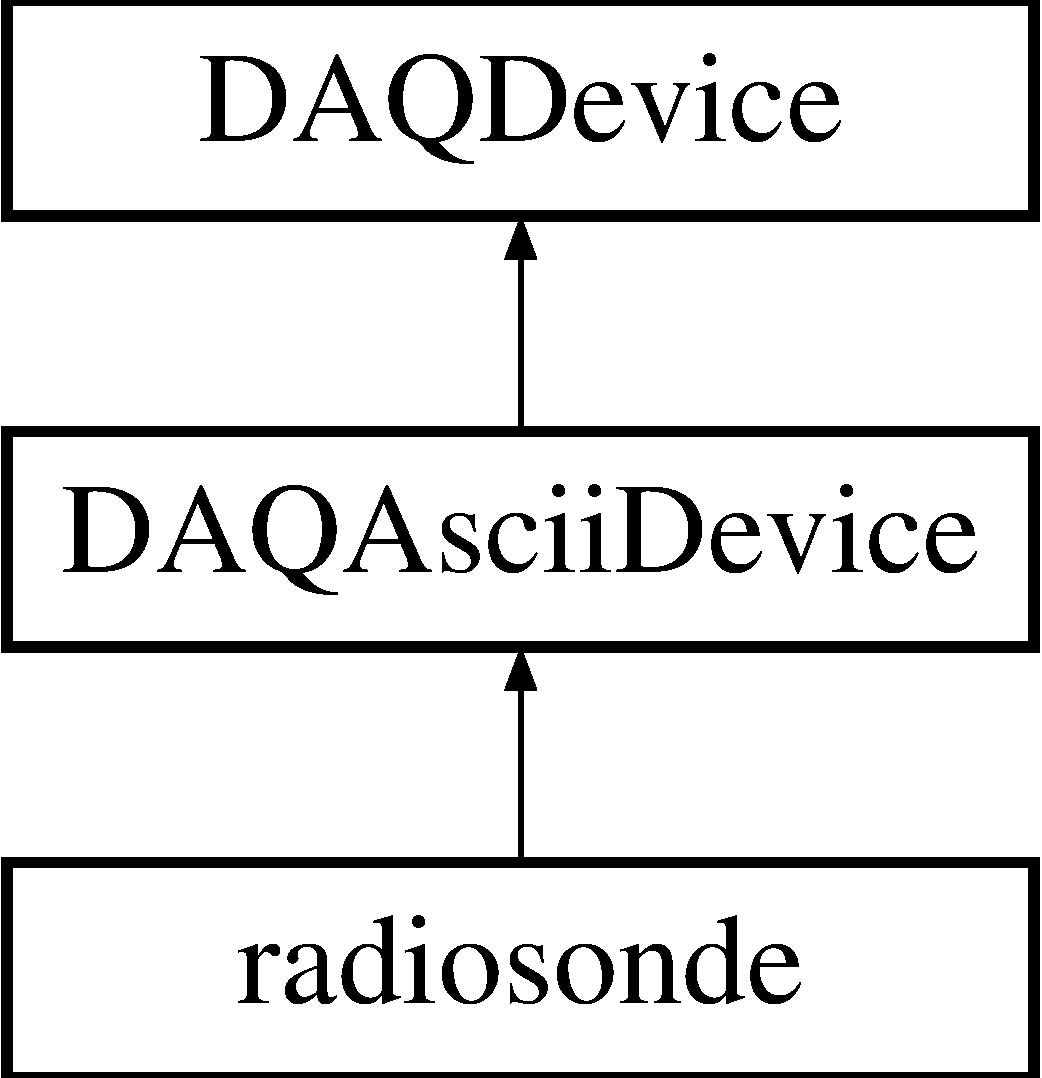
\includegraphics[height=3.000000cm]{classradiosonde}
\end{center}
\end{figure}
\subsection*{Public Member Functions}
\begin{DoxyCompactItemize}
\item 
\hyperlink{classradiosonde_aeee339fb1fefca43181050022a115950}{radiosonde} ()
\item 
\hyperlink{classradiosonde_a215f03d8d6d94f97989770f703549dc7}{$\sim$radiosonde} ()
\item 
void \hyperlink{classradiosonde_a8c1c1be9e950d6c3b70df6bc13f8cbca}{set\-Config\-Defaults} ()
\item 
int \hyperlink{classradiosonde_ad8974221a2a65698387b7c6552f6903a}{read\-Header} (const char $\ast$\hyperlink{classDAQDevice_a7f9cda7cf5b41f6b134c313477e9644b}{filename})
\item 
int \hyperlink{classradiosonde_af31298e5aa292b7d8113116ae112db01}{parse\-Data} (char $\ast$line, struct timeval $\ast$l\-\_\-t\-Data, double $\ast$\hyperlink{classDAQDevice_ad148188c57598fdf4fd4c1c333aeb0d8}{sensor\-Value})
\item 
unsigned int \hyperlink{classradiosonde_ad7e2421821dca49851d8fc8c5f9f3177}{get\-Sensor\-Group} ()
\end{DoxyCompactItemize}
\subsection*{Private Attributes}
\begin{DoxyCompactItemize}
\item 
struct timeval \hyperlink{classradiosonde_a3a7487275417bf085aed3f7e8bb9efdd}{start\-\_\-time}
\end{DoxyCompactItemize}
\subsection*{Additional Inherited Members}


\subsection{Constructor \& Destructor Documentation}
\hypertarget{classradiosonde_aeee339fb1fefca43181050022a115950}{\index{radiosonde@{radiosonde}!radiosonde@{radiosonde}}
\index{radiosonde@{radiosonde}!radiosonde@{radiosonde}}
\subsubsection[{radiosonde}]{\setlength{\rightskip}{0pt plus 5cm}radiosonde\-::radiosonde (
\begin{DoxyParamCaption}
{}
\end{DoxyParamCaption}
)}}\label{classradiosonde_aeee339fb1fefca43181050022a115950}
\hypertarget{classradiosonde_a215f03d8d6d94f97989770f703549dc7}{\index{radiosonde@{radiosonde}!$\sim$radiosonde@{$\sim$radiosonde}}
\index{$\sim$radiosonde@{$\sim$radiosonde}!radiosonde@{radiosonde}}
\subsubsection[{$\sim$radiosonde}]{\setlength{\rightskip}{0pt plus 5cm}radiosonde\-::$\sim$radiosonde (
\begin{DoxyParamCaption}
{}
\end{DoxyParamCaption}
)}}\label{classradiosonde_a215f03d8d6d94f97989770f703549dc7}


\subsection{Member Function Documentation}
\hypertarget{classradiosonde_ad7e2421821dca49851d8fc8c5f9f3177}{\index{radiosonde@{radiosonde}!get\-Sensor\-Group@{get\-Sensor\-Group}}
\index{get\-Sensor\-Group@{get\-Sensor\-Group}!radiosonde@{radiosonde}}
\subsubsection[{get\-Sensor\-Group}]{\setlength{\rightskip}{0pt plus 5cm}unsigned int radiosonde\-::get\-Sensor\-Group (
\begin{DoxyParamCaption}
{}
\end{DoxyParamCaption}
)\hspace{0.3cm}{\ttfamily [virtual]}}}\label{classradiosonde_ad7e2421821dca49851d8fc8c5f9f3177}
Define a sensor group number for all the availble sensor group files 

Reimplemented from \hyperlink{classDAQDevice_a61d08492a11c30944dfaf3b86115abe8}{D\-A\-Q\-Device}.

\hypertarget{classradiosonde_af31298e5aa292b7d8113116ae112db01}{\index{radiosonde@{radiosonde}!parse\-Data@{parse\-Data}}
\index{parse\-Data@{parse\-Data}!radiosonde@{radiosonde}}
\subsubsection[{parse\-Data}]{\setlength{\rightskip}{0pt plus 5cm}int radiosonde\-::parse\-Data (
\begin{DoxyParamCaption}
\item[{char $\ast$}]{line, }
\item[{struct timeval $\ast$}]{l\-\_\-t\-Data, }
\item[{double $\ast$}]{sensor\-Value}
\end{DoxyParamCaption}
)\hspace{0.3cm}{\ttfamily [virtual]}}}\label{classradiosonde_af31298e5aa292b7d8113116ae112db01}
Read the data from the current line of the data file. \begin{DoxyReturn}{Returns}
-\/1 no data found, skip storage 0 sucess, store data, 1 read another line 
\end{DoxyReturn}


Reimplemented from \hyperlink{classDAQAsciiDevice_a9c20d9d69af4ba1641dbc82dd5be2aa5}{D\-A\-Q\-Ascii\-Device}.

\hypertarget{classradiosonde_ad8974221a2a65698387b7c6552f6903a}{\index{radiosonde@{radiosonde}!read\-Header@{read\-Header}}
\index{read\-Header@{read\-Header}!radiosonde@{radiosonde}}
\subsubsection[{read\-Header}]{\setlength{\rightskip}{0pt plus 5cm}int radiosonde\-::read\-Header (
\begin{DoxyParamCaption}
\item[{const char $\ast$}]{header}
\end{DoxyParamCaption}
)\hspace{0.3cm}{\ttfamily [virtual]}}}\label{classradiosonde_ad8974221a2a65698387b7c6552f6903a}
Get time until next sample and it's id 

Reimplemented from \hyperlink{classDAQAsciiDevice_a5fce725c52b70ef2f56a34b32a03e15d}{D\-A\-Q\-Ascii\-Device}.

\hypertarget{classradiosonde_a8c1c1be9e950d6c3b70df6bc13f8cbca}{\index{radiosonde@{radiosonde}!set\-Config\-Defaults@{set\-Config\-Defaults}}
\index{set\-Config\-Defaults@{set\-Config\-Defaults}!radiosonde@{radiosonde}}
\subsubsection[{set\-Config\-Defaults}]{\setlength{\rightskip}{0pt plus 5cm}void radiosonde\-::set\-Config\-Defaults (
\begin{DoxyParamCaption}
{}
\end{DoxyParamCaption}
)\hspace{0.3cm}{\ttfamily [virtual]}}}\label{classradiosonde_a8c1c1be9e950d6c3b70df6bc13f8cbca}
The function is called before reading the configuration from the inifile. Use this fucntion in the module specific implementation to override the standard defaults 

Reimplemented from \hyperlink{classDAQDevice_a7685cec80865752cc0ef3ab49c6c2277}{D\-A\-Q\-Device}.



\subsection{Member Data Documentation}
\hypertarget{classradiosonde_a3a7487275417bf085aed3f7e8bb9efdd}{\index{radiosonde@{radiosonde}!start\-\_\-time@{start\-\_\-time}}
\index{start\-\_\-time@{start\-\_\-time}!radiosonde@{radiosonde}}
\subsubsection[{start\-\_\-time}]{\setlength{\rightskip}{0pt plus 5cm}struct timeval radiosonde\-::start\-\_\-time\hspace{0.3cm}{\ttfamily [private]}}}\label{classradiosonde_a3a7487275417bf085aed3f7e8bb9efdd}


The documentation for this class was generated from the following files\-:\begin{DoxyCompactItemize}
\item 
/home/ntj/\-Development/phd/kitcube-\/tools/src/kitcube-\/devices/\hyperlink{radiosonde_8h}{radiosonde.\-h}\item 
/home/ntj/\-Development/phd/kitcube-\/tools/src/kitcube-\/devices/\hyperlink{radiosonde_8cpp}{radiosonde.\-cpp}\end{DoxyCompactItemize}

\hypertarget{classReader}{\section{Reader Class Reference}
\label{classReader}\index{Reader@{Reader}}
}


{\ttfamily \#include $<$reader.\-h$>$}

Inheritance diagram for Reader\-:\begin{figure}[H]
\begin{center}
\leavevmode
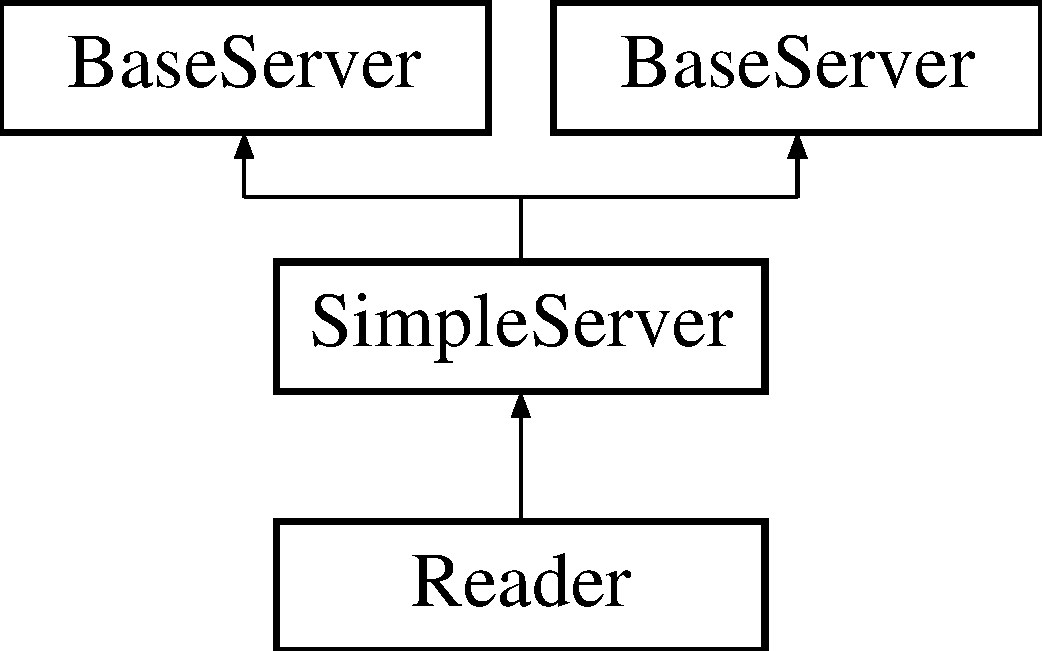
\includegraphics[height=3.000000cm]{classReader}
\end{center}
\end{figure}
\subsection*{Public Member Functions}
\begin{DoxyCompactItemize}
\item 
\hyperlink{classReader_adcda31b507720ab44044d7a21686fba2}{Reader} ()
\item 
\hyperlink{classReader_a78089542fd27a0ac2df6702fffe8725c}{$\sim$\-Reader} ()
\item 
void \hyperlink{classReader_a00b096fb45b4c2510f8b045989bf162c}{set\-App\-Name} (const char $\ast$name)
\item 
int \hyperlink{classReader_ae309d831a357a1107a7f7f1db49f00e8}{get\-App\-Id} ()
\item 
void \hyperlink{classReader_aadf658dbddd5060d8a2f10482f070a16}{set\-Reset} ()
\item 
void \hyperlink{classReader_a0f1f72184f82854b67b28471844734da}{read\-Inifile} (const char $\ast$\hyperlink{classReader_aaeaf0ff38217063a14b00bf16deed50a}{inifile}, const char $\ast$module=0)
\item 
void \hyperlink{classReader_a4f2113dc609befa174f3716492bf7ebc}{run\-As\-Daemon} (bool flag=true)
\item 
void \hyperlink{classReader_aa471d16ce98f57c1c40aaf6090a3a971}{get\-Next\-Sample} (int $\ast$i\-Sample, double $\ast$t\-Wait)
\item 
void \hyperlink{classReader_a656b1bef6050e0b043f4499fe2a22f2d}{get\-Next\-Sample} (int $\ast$i\-Sample, struct timeval $\ast$t\-Wait)
\item 
int \hyperlink{classReader_a1c23cb1e3ec1a87fb5db65392fb43d21}{handle\-\_\-timeout} ()
\item 
int \hyperlink{classReader_a8adf1a4f5f852efa0433cab70bb750c0}{read\-\_\-from\-\_\-keyboard} ()
\item 
void \hyperlink{classReader_a8d71e1068d9bf3886ac4fd472ed71ae9}{execute\-Cmd} (int client, short cmd, unsigned int $\ast$arg, short n)
\item 
void \hyperlink{classReader_a966aeba64f6a646c10276d248b60760c}{run\-Readout} ()
\item 
long int \hyperlink{classReader_a1abd8f689645dafbf76fda50cd9dd48d}{analyse\-Timing} (struct timeval $\ast$t)
\item 
void \hyperlink{classReader_a73c6e0134bdd06ebdbfef68252b8be94}{display\-Status} (F\-I\-L\-E $\ast$\hyperlink{classBaseServer_a9ad43261a042fbeeafee33ca4c0b3fd3}{fout})
\item 
void \hyperlink{classReader_a330c1515ec85cdde0662805cd3be735e}{analyse\-Disk\-Space} (const char $\ast$dir)
\end{DoxyCompactItemize}
\subsection*{Private Attributes}
\begin{DoxyCompactItemize}
\item 
int \hyperlink{classReader_ae5710fab671a39e2e2c6472aa8cd5cf6}{app\-Id}
\item 
bool \hyperlink{classReader_ac7fb1595fa93f70c58656bff11091f94}{reset}
\item 
std\-::string \hyperlink{classReader_a6207e38c6bc804dabb6b086405c8231d}{app\-Name}
\item 
bool \hyperlink{classReader_a08302c0ae536dd0d0d2de37143eb7a94}{run\-Daemon}
\item 
int \hyperlink{classReader_abe8094976b8f244a539e34689dda91bc}{t\-Sample\-From\-Inifile}
\item 
int \hyperlink{classReader_abf76426a02d8896908e76edefa1821b2}{n\-Modules}
\item 
std\-::string \hyperlink{classReader_a0120f495d8251090cb5a406b6326c543}{module\-Name}
\item 
std\-::string $\ast$ \hyperlink{classReader_a082c78fbd3e67423e6ab134d4fb61cc9}{module\-Type}
\item 
int $\ast$ \hyperlink{classReader_aa816d9ed493e53da3119680a60a581ed}{module\-Number}
\item 
std\-::string $\ast$ \hyperlink{classReader_ab53774f0eac672c5d80f5f086e7b0d3b}{ini\-Group}
\item 
\hyperlink{classDAQDevice}{D\-A\-Q\-Device} $\ast$$\ast$ \hyperlink{classReader_a759e4aca2327cd6959af3273bb10c979}{dev}
\item 
\hyperlink{classSysLog}{Sys\-Log} $\ast$ \hyperlink{classReader_a3623b291506e1e6f54b90e00eeefdad8}{log}
\item 
int \hyperlink{classReader_a5d275c3577f7d7c02a6cc83f70d0dcc7}{n\-Error}
\item 
int \hyperlink{classReader_aa87a2b5443237f58cadeaa815e6e6790}{n\-Groups}
\item 
unsigned long \hyperlink{classReader_aa6c9e0275ed3601e6df4fcb194d97834}{samples\-N}
\item 
long long \hyperlink{classReader_a85c71a4d9f959cabea9cb7b168d966a0}{timing\-N}
\item 
long long \hyperlink{classReader_ab185760a9e7235b20f9cb21db44d0663}{timing\-Sum}
\item 
long long \hyperlink{classReader_a8a8de149490f7fe3c01413453c3d0a50}{timing\-Sum2}
\item 
long long \hyperlink{classReader_a6e85a422cbe42ab60c20b06e719bbdae}{timing\-Min}
\item 
long long \hyperlink{classReader_a6cf0d42c4478dafaf61696bcc0c668f9}{timing\-Max}
\item 
int \hyperlink{classReader_a4b6268d4969e7209ea2c7fea25d09a58}{n\-Samples\-Skipped}
\item 
\hyperlink{classSimpleSocket}{Simple\-Socket} $\ast$ \hyperlink{classReader_a4cbb3ab4b903d0114ee8f6ea521259b8}{cfp\-Sock}
\item 
std\-::string \hyperlink{classReader_aaeaf0ff38217063a14b00bf16deed50a}{inifile}
\item 
std\-::string \hyperlink{classReader_a527aa131b2bafc4f6292828ac097a77f}{filename}
\item 
std\-::string \hyperlink{classReader_af4873d08f7454f94b69379682b86b761}{filename\-Tmpl}
\item 
std\-::string \hyperlink{classReader_ace3793e1d270276c63e9689e59a6cb23}{basedir}
\item 
std\-::string \hyperlink{classReader_a5357e56eb1aea6d31962a3ac034b4d0b}{basedir\-Tmpl}
\item 
int \hyperlink{classReader_a2f8737a95888b1cb41b2fa191382fe1c}{location\-Id}
\item 
std\-::string \hyperlink{classReader_a8f238308360fe50adda67d360a9d3b28}{location}
\item 
int \hyperlink{classReader_a2df27c47ac46939a756ab78b71690d44}{unique\-Id}
\item 
F\-I\-L\-E $\ast$ \hyperlink{classReader_aa0296167e6f6781808727fa2a93b6a74}{bg\-File}
\item 
bool \hyperlink{classReader_acfb61762011f4aa995126c9e8c1950c3}{record}
\item 
int \hyperlink{classReader_a298c2e5e5d77eab7642ebfef4ac8e8da}{sel\-Store}
\item 
int \hyperlink{classReader_ab52320900b9165867a7294a5282b2caf}{sel\-Display}
\item 
int \hyperlink{classReader_a822ff7808145dd73c18e03a02ff59fbe}{sel\-Telescopes}
\item 
int \hyperlink{classReader_a04a91fc12dab5c7eee7bcbf051619b16}{limit\-Var}
\item 
unsigned long \hyperlink{classReader_a98d0f293c15366f1efbe6722ed4fa9eb}{stat\-Samples}
\item 
unsigned long \hyperlink{classReader_a8fd2d0cd7df8a4c2cf1ca350f6ca95c9}{stat\-Offset}
\item 
unsigned long \hyperlink{classReader_ac749831ff1afb95fcc67c3100b45c6d7}{disabled\-Pixel} \mbox{[}20\mbox{]}
\item 
unsigned long \hyperlink{classReader_a03046b6de7c2adc07bc85fffd69d78b1}{pixel\-Status} \mbox{[}20\mbox{]}\mbox{[}24\mbox{]}
\item 
unsigned long \hyperlink{classReader_a59ce0afb9461ba7360d135e4b2c4fb95}{fddas\-Run\-Id}
\item 
std\-::string \hyperlink{classReader_a7e985019f1cb999712f0955e0febf4ef}{bgrun\-File}
\item 
std\-::string \hyperlink{classReader_a097598eeea105530aa64222c8bf6d828}{bgcal\-File}
\item 
int \hyperlink{classReader_a1fa6f7582327f96076165c7b95b55a1b}{bgrun\-T\-Sample}
\item 
int \hyperlink{classReader_aa98bab20153537c112ca0640c210c34b}{bgcal\-T\-Sample}
\item 
F\-I\-L\-E $\ast$ \hyperlink{classReader_adced1caed365fc651778f352416914c6}{flog}
\item 
std\-::string \hyperlink{classReader_a59413e43dd39a74095478580bdcc7eb9}{logfile}
\item 
int \hyperlink{classReader_a3fb6ef9d55ca8c9d23e0bf6be5796583}{run\-Mode}
\item 
std\-::string \hyperlink{classReader_a25348aba8ec875045f557beaa11e2415}{run\-Type}
\item 
int \hyperlink{classReader_aaa48504eb00d9023ff126beb8b6f5c89}{tel\-Active} \mbox{[}24\mbox{]}
\item 
unsigned long \hyperlink{classReader_a14d16a29a867041a4bc916142630a162}{last\-Data\-Sec} \mbox{[}24\mbox{]}
\item 
int \hyperlink{classReader_a19a9f80856c30d86a31b79f1672b3804}{hitrate\-Overflow} \mbox{[}24\mbox{]}
\item 
unsigned long \hyperlink{classReader_a9686e0c5ed311baa141f6021fc45c931}{last\-Second\-Diff} \mbox{[}24\mbox{]}
\item 
int \hyperlink{classReader_a57a28f21905a04e6eeb0008840ed7ab6}{variance\-Level} \mbox{[}24\mbox{]}
\item 
float \hyperlink{classReader_a2318276c2913fe9eb87c1b49c786d9b5}{variance\-Closed\-Shutter}
\item 
float \hyperlink{classReader_a55a312840dc5e05cbadcc8002838a252}{variance\-Overflow}
\item 
int \hyperlink{classReader_aa69150af33df50c03662851a660321b4}{last\-Variance} \mbox{[}24\mbox{]}
\item 
int \hyperlink{classReader_a20de0ffe57bd63c8b322a552d0eea7aa}{actual\-Variance} \mbox{[}24\mbox{]}
\item 
unsigned long \hyperlink{classReader_a17df32c8ae16df4d276d73b8d955c0e6}{last\-Time\-Stamp}
\item 
unsigned long \hyperlink{classReader_a0f8a298ecdd8c02e9e1a428c1634581c}{actual\-Time\-Stamp}
\item 
int \hyperlink{classReader_ae79b47c731fc265b3ca401cdbdccd726}{threshold\-Level} \mbox{[}24\mbox{]}
\item 
int \hyperlink{classReader_a9574d13bbda6fd1a17f1aca61e2a0df1}{missing\-Tel} \mbox{[}24\mbox{]}
\item 
int \hyperlink{classReader_a92b7378790ac975b65f159b6502cb47e}{error\-Level} \mbox{[}24\mbox{]}
\item 
int \hyperlink{classReader_ae6d9d7dae0b2b71985a8d2df2ee09819}{error\-General}
\item 
unsigned long long \hyperlink{classReader_ad7344b65bf38e5ea1a22230ad37fc95a}{last\-Deadtime} \mbox{[}24\mbox{]}
\item 
int \hyperlink{classReader_aee93b4550b1f413ac5e263e0a2f85b25}{deadtime\-Active} \mbox{[}24\mbox{]}
\item 
int \hyperlink{classReader_aeb5766561480656c2a2182b86e2cdae8}{t\-Database}
\item 
std\-::string \hyperlink{classReader_ad92d8d94dae6b66a5278cb792ca0a206}{qd\-Path}
\item 
std\-::string \hyperlink{classReader_ab0da569b087b0ba5efdb22ee8459e40d}{qd\-Config}
\item 
int \hyperlink{classReader_a69f380acc4c2b439f1cd940b12349d92}{qd\-T\-Sample}
\item 
int \hyperlink{classReader_a1807cf089712f144cbf20b280dc36240}{qd\-N\-Sensors}
\item 
double \hyperlink{classReader_a0746e7e813a05ee8648875ee2776b5f4}{disk\-\_\-avail\-\_\-gb}
\item 
struct timeval \hyperlink{classReader_a4b26c73a9ce2d08fd78b11dca25c0ad6}{time\-\_\-now}
\item 
uint64\-\_\-t \hyperlink{classReader_a759fcd53649d1d49e66ff8e9cfd4b452}{rx}
\item 
uint64\-\_\-t \hyperlink{classReader_acb6c6053d7bd278014e04c34fdad4e0e}{tx}
\end{DoxyCompactItemize}
\subsection*{Additional Inherited Members}


\subsection{Detailed Description}
\begin{DoxyVerb}The reader funtion periodically transfers data from the 
connected DAQ systems and writes any newly recorded data 
to the database. At the same time also some indicators 
for the system performance are stored in a separate 
table. The performance data contains:
 - Amount of free data
 - Rate of stored data
 - Rate of transfered data (send/receive)
 - Durations for data transfer an database access
 - Timing acurancy of the scheduler

The reader class is using several debug levels to control the
amount of messages send to the terminal. 

0: Only output of application welcome and error messages
1: Additional output of new files that are porcessed
2: Display of key information of every reader loop
3: Header information of every function called
4+5: More messages


The following box shows a sample call of the background recorder.
\end{DoxyVerb}
 \begin{DoxyVerb}  TsBackgroundLoop *bgrec;
  Pbus *thePbus;

  Pbus::init(inifile.c_str());


  // Create recorder
  bgrec = new TsBackgroundLoop();
  bgrec->readInifile(inifile.c_str());

  bgrec->setLogfile(stdout);

  // Set parameter: Period length, selected parameter, file, ....
  bgrec->setParameter(name, tSample, 0, selRecord, selDisplay, runType.c_str());  // no output to file, take data every 5s

  // Run background recorder
  // The readout process is started at all connected telescopes
  bgrec->runReadout(stdout);

  delete bgrec;
\end{DoxyVerb}
 

\subsection{Constructor \& Destructor Documentation}
\hypertarget{classReader_adcda31b507720ab44044d7a21686fba2}{\index{Reader@{Reader}!Reader@{Reader}}
\index{Reader@{Reader}!Reader@{Reader}}
\subsubsection[{Reader}]{\setlength{\rightskip}{0pt plus 5cm}Reader\-::\-Reader (
\begin{DoxyParamCaption}
{}
\end{DoxyParamCaption}
)}}\label{classReader_adcda31b507720ab44044d7a21686fba2}
\hypertarget{classReader_a78089542fd27a0ac2df6702fffe8725c}{\index{Reader@{Reader}!$\sim$\-Reader@{$\sim$\-Reader}}
\index{$\sim$\-Reader@{$\sim$\-Reader}!Reader@{Reader}}
\subsubsection[{$\sim$\-Reader}]{\setlength{\rightskip}{0pt plus 5cm}Reader\-::$\sim$\-Reader (
\begin{DoxyParamCaption}
{}
\end{DoxyParamCaption}
)}}\label{classReader_a78089542fd27a0ac2df6702fffe8725c}


\subsection{Member Function Documentation}
\hypertarget{classReader_a330c1515ec85cdde0662805cd3be735e}{\index{Reader@{Reader}!analyse\-Disk\-Space@{analyse\-Disk\-Space}}
\index{analyse\-Disk\-Space@{analyse\-Disk\-Space}!Reader@{Reader}}
\subsubsection[{analyse\-Disk\-Space}]{\setlength{\rightskip}{0pt plus 5cm}void Reader\-::analyse\-Disk\-Space (
\begin{DoxyParamCaption}
\item[{const char $\ast$}]{dir}
\end{DoxyParamCaption}
)}}\label{classReader_a330c1515ec85cdde0662805cd3be735e}
Read the free disk space from the filesystem that is used for data storage. \hypertarget{classReader_a1abd8f689645dafbf76fda50cd9dd48d}{\index{Reader@{Reader}!analyse\-Timing@{analyse\-Timing}}
\index{analyse\-Timing@{analyse\-Timing}!Reader@{Reader}}
\subsubsection[{analyse\-Timing}]{\setlength{\rightskip}{0pt plus 5cm}long int Reader\-::analyse\-Timing (
\begin{DoxyParamCaption}
\item[{struct timeval $\ast$}]{t}
\end{DoxyParamCaption}
)}}\label{classReader_a1abd8f689645dafbf76fda50cd9dd48d}
Analyse timing \hypertarget{classReader_a73c6e0134bdd06ebdbfef68252b8be94}{\index{Reader@{Reader}!display\-Status@{display\-Status}}
\index{display\-Status@{display\-Status}!Reader@{Reader}}
\subsubsection[{display\-Status}]{\setlength{\rightskip}{0pt plus 5cm}void Reader\-::display\-Status (
\begin{DoxyParamCaption}
\item[{F\-I\-L\-E $\ast$}]{fout}
\end{DoxyParamCaption}
)}}\label{classReader_a73c6e0134bdd06ebdbfef68252b8be94}
Display status of readout process \hypertarget{classReader_a8d71e1068d9bf3886ac4fd472ed71ae9}{\index{Reader@{Reader}!execute\-Cmd@{execute\-Cmd}}
\index{execute\-Cmd@{execute\-Cmd}!Reader@{Reader}}
\subsubsection[{execute\-Cmd}]{\setlength{\rightskip}{0pt plus 5cm}void Reader\-::execute\-Cmd (
\begin{DoxyParamCaption}
\item[{int}]{client, }
\item[{short}]{cmd, }
\item[{unsigned int $\ast$}]{arg, }
\item[{short}]{n}
\end{DoxyParamCaption}
)\hspace{0.3cm}{\ttfamily [virtual]}}}\label{classReader_a8d71e1068d9bf3886ac4fd472ed71ae9}
Execute the command 

Reimplemented from \hyperlink{classSimpleServer_ad8244094d9e1806edaa166093c94bd24}{Simple\-Server}.

\hypertarget{classReader_ae309d831a357a1107a7f7f1db49f00e8}{\index{Reader@{Reader}!get\-App\-Id@{get\-App\-Id}}
\index{get\-App\-Id@{get\-App\-Id}!Reader@{Reader}}
\subsubsection[{get\-App\-Id}]{\setlength{\rightskip}{0pt plus 5cm}int Reader\-::get\-App\-Id (
\begin{DoxyParamCaption}
{}
\end{DoxyParamCaption}
)}}\label{classReader_ae309d831a357a1107a7f7f1db49f00e8}
Get the number of the application \hypertarget{classReader_aa471d16ce98f57c1c40aaf6090a3a971}{\index{Reader@{Reader}!get\-Next\-Sample@{get\-Next\-Sample}}
\index{get\-Next\-Sample@{get\-Next\-Sample}!Reader@{Reader}}
\subsubsection[{get\-Next\-Sample}]{\setlength{\rightskip}{0pt plus 5cm}void Reader\-::get\-Next\-Sample (
\begin{DoxyParamCaption}
\item[{int $\ast$}]{i\-Sample, }
\item[{double $\ast$}]{t\-Wait}
\end{DoxyParamCaption}
)}}\label{classReader_aa471d16ce98f57c1c40aaf6090a3a971}
Get time until next sample and it's id \hypertarget{classReader_a656b1bef6050e0b043f4499fe2a22f2d}{\index{Reader@{Reader}!get\-Next\-Sample@{get\-Next\-Sample}}
\index{get\-Next\-Sample@{get\-Next\-Sample}!Reader@{Reader}}
\subsubsection[{get\-Next\-Sample}]{\setlength{\rightskip}{0pt plus 5cm}void Reader\-::get\-Next\-Sample (
\begin{DoxyParamCaption}
\item[{int $\ast$}]{i\-Sample, }
\item[{struct timeval $\ast$}]{t\-Wait}
\end{DoxyParamCaption}
)}}\label{classReader_a656b1bef6050e0b043f4499fe2a22f2d}
\hypertarget{classReader_a1c23cb1e3ec1a87fb5db65392fb43d21}{\index{Reader@{Reader}!handle\-\_\-timeout@{handle\-\_\-timeout}}
\index{handle\-\_\-timeout@{handle\-\_\-timeout}!Reader@{Reader}}
\subsubsection[{handle\-\_\-timeout}]{\setlength{\rightskip}{0pt plus 5cm}int Reader\-::handle\-\_\-timeout (
\begin{DoxyParamCaption}
{}
\end{DoxyParamCaption}
)\hspace{0.3cm}{\ttfamily [virtual]}}}\label{classReader_a1c23cb1e3ec1a87fb5db65392fb43d21}
Handler for the timeout 

Reimplemented from \hyperlink{classBaseServer_a892cf59b889f59d73031108cfab07772}{Base\-Server}.

\hypertarget{classReader_a8adf1a4f5f852efa0433cab70bb750c0}{\index{Reader@{Reader}!read\-\_\-from\-\_\-keyboard@{read\-\_\-from\-\_\-keyboard}}
\index{read\-\_\-from\-\_\-keyboard@{read\-\_\-from\-\_\-keyboard}!Reader@{Reader}}
\subsubsection[{read\-\_\-from\-\_\-keyboard}]{\setlength{\rightskip}{0pt plus 5cm}int Reader\-::read\-\_\-from\-\_\-keyboard (
\begin{DoxyParamCaption}
{}
\end{DoxyParamCaption}
)\hspace{0.3cm}{\ttfamily [virtual]}}}\label{classReader_a8adf1a4f5f852efa0433cab70bb750c0}
Keyboard interface for interactive control (only for compatibility reasons 

Reimplemented from \hyperlink{classBaseServer_a2c5a73b3bd9950a7809ac2a353061960}{Base\-Server}.

\hypertarget{classReader_a0f1f72184f82854b67b28471844734da}{\index{Reader@{Reader}!read\-Inifile@{read\-Inifile}}
\index{read\-Inifile@{read\-Inifile}!Reader@{Reader}}
\subsubsection[{read\-Inifile}]{\setlength{\rightskip}{0pt plus 5cm}void Reader\-::read\-Inifile (
\begin{DoxyParamCaption}
\item[{const char $\ast$}]{inifile, }
\item[{const char $\ast$}]{module = {\ttfamily 0}}
\end{DoxyParamCaption}
)}}\label{classReader_a0f1f72184f82854b67b28471844734da}
Read parameter from inifile. The module definition will be read from the argument list, afterwards from the reader section in the inifile and at last the default name (Simulation) selected. \hypertarget{classReader_a4f2113dc609befa174f3716492bf7ebc}{\index{Reader@{Reader}!run\-As\-Daemon@{run\-As\-Daemon}}
\index{run\-As\-Daemon@{run\-As\-Daemon}!Reader@{Reader}}
\subsubsection[{run\-As\-Daemon}]{\setlength{\rightskip}{0pt plus 5cm}void Reader\-::run\-As\-Daemon (
\begin{DoxyParamCaption}
\item[{bool}]{flag = {\ttfamily true}}
\end{DoxyParamCaption}
)}}\label{classReader_a4f2113dc609befa174f3716492bf7ebc}
Set operation without interactive inputs \hypertarget{classReader_a966aeba64f6a646c10276d248b60760c}{\index{Reader@{Reader}!run\-Readout@{run\-Readout}}
\index{run\-Readout@{run\-Readout}!Reader@{Reader}}
\subsubsection[{run\-Readout}]{\setlength{\rightskip}{0pt plus 5cm}void Reader\-::run\-Readout (
\begin{DoxyParamCaption}
{}
\end{DoxyParamCaption}
)}}\label{classReader_a966aeba64f6a646c10276d248b60760c}
Start the server and all the client recording the telescopes background data. \hypertarget{classReader_a00b096fb45b4c2510f8b045989bf162c}{\index{Reader@{Reader}!set\-App\-Name@{set\-App\-Name}}
\index{set\-App\-Name@{set\-App\-Name}!Reader@{Reader}}
\subsubsection[{set\-App\-Name}]{\setlength{\rightskip}{0pt plus 5cm}void Reader\-::set\-App\-Name (
\begin{DoxyParamCaption}
\item[{const char $\ast$}]{name}
\end{DoxyParamCaption}
)}}\label{classReader_a00b096fb45b4c2510f8b045989bf162c}
Change the default name of the application used to figure out the right inifile section \hypertarget{classReader_aadf658dbddd5060d8a2f10482f070a16}{\index{Reader@{Reader}!set\-Reset@{set\-Reset}}
\index{set\-Reset@{set\-Reset}!Reader@{Reader}}
\subsubsection[{set\-Reset}]{\setlength{\rightskip}{0pt plus 5cm}void Reader\-::set\-Reset (
\begin{DoxyParamCaption}
{}
\end{DoxyParamCaption}
)}}\label{classReader_aadf658dbddd5060d8a2f10482f070a16}
Activate reset of file pointers 

\subsection{Member Data Documentation}
\hypertarget{classReader_a0f8a298ecdd8c02e9e1a428c1634581c}{\index{Reader@{Reader}!actual\-Time\-Stamp@{actual\-Time\-Stamp}}
\index{actual\-Time\-Stamp@{actual\-Time\-Stamp}!Reader@{Reader}}
\subsubsection[{actual\-Time\-Stamp}]{\setlength{\rightskip}{0pt plus 5cm}unsigned long Reader\-::actual\-Time\-Stamp\hspace{0.3cm}{\ttfamily [private]}}}\label{classReader_a0f8a298ecdd8c02e9e1a428c1634581c}
Actual time stamp \hypertarget{classReader_a20de0ffe57bd63c8b322a552d0eea7aa}{\index{Reader@{Reader}!actual\-Variance@{actual\-Variance}}
\index{actual\-Variance@{actual\-Variance}!Reader@{Reader}}
\subsubsection[{actual\-Variance}]{\setlength{\rightskip}{0pt plus 5cm}int Reader\-::actual\-Variance\mbox{[}24\mbox{]}\hspace{0.3cm}{\ttfamily [private]}}}\label{classReader_a20de0ffe57bd63c8b322a552d0eea7aa}
Array with the actual variances \hypertarget{classReader_ae5710fab671a39e2e2c6472aa8cd5cf6}{\index{Reader@{Reader}!app\-Id@{app\-Id}}
\index{app\-Id@{app\-Id}!Reader@{Reader}}
\subsubsection[{app\-Id}]{\setlength{\rightskip}{0pt plus 5cm}int Reader\-::app\-Id\hspace{0.3cm}{\ttfamily [private]}}}\label{classReader_ae5710fab671a39e2e2c6472aa8cd5cf6}
Get index / time stamp of a folder or a filename. The index field is defined by a starting tag directly before the numerical values. The length of the field can be given by a final string of the length of the field or all following digit will be taken. In case of success the parsed numerical values will cut out of the passed filename.\-Get list of new files Read new data from the file Every reader application has it's own I\-D \hypertarget{classReader_a6207e38c6bc804dabb6b086405c8231d}{\index{Reader@{Reader}!app\-Name@{app\-Name}}
\index{app\-Name@{app\-Name}!Reader@{Reader}}
\subsubsection[{app\-Name}]{\setlength{\rightskip}{0pt plus 5cm}std\-::string Reader\-::app\-Name\hspace{0.3cm}{\ttfamily [private]}}}\label{classReader_a6207e38c6bc804dabb6b086405c8231d}
Name of the application. Used to select the application ini group. Default\-: \hyperlink{classReader}{Reader} \hypertarget{classReader_ace3793e1d270276c63e9689e59a6cb23}{\index{Reader@{Reader}!basedir@{basedir}}
\index{basedir@{basedir}!Reader@{Reader}}
\subsubsection[{basedir}]{\setlength{\rightskip}{0pt plus 5cm}std\-::string Reader\-::basedir\hspace{0.3cm}{\ttfamily [private]}}}\label{classReader_ace3793e1d270276c63e9689e59a6cb23}
Basedir of the auger file \hypertarget{classReader_a5357e56eb1aea6d31962a3ac034b4d0b}{\index{Reader@{Reader}!basedir\-Tmpl@{basedir\-Tmpl}}
\index{basedir\-Tmpl@{basedir\-Tmpl}!Reader@{Reader}}
\subsubsection[{basedir\-Tmpl}]{\setlength{\rightskip}{0pt plus 5cm}std\-::string Reader\-::basedir\-Tmpl\hspace{0.3cm}{\ttfamily [private]}}}\label{classReader_a5357e56eb1aea6d31962a3ac034b4d0b}
Template for the basedir of the auger file \hypertarget{classReader_a097598eeea105530aa64222c8bf6d828}{\index{Reader@{Reader}!bgcal\-File@{bgcal\-File}}
\index{bgcal\-File@{bgcal\-File}!Reader@{Reader}}
\subsubsection[{bgcal\-File}]{\setlength{\rightskip}{0pt plus 5cm}std\-::string Reader\-::bgcal\-File\hspace{0.3cm}{\ttfamily [private]}}}\label{classReader_a097598eeea105530aa64222c8bf6d828}
Filename template for the calibration mode \hypertarget{classReader_aa98bab20153537c112ca0640c210c34b}{\index{Reader@{Reader}!bgcal\-T\-Sample@{bgcal\-T\-Sample}}
\index{bgcal\-T\-Sample@{bgcal\-T\-Sample}!Reader@{Reader}}
\subsubsection[{bgcal\-T\-Sample}]{\setlength{\rightskip}{0pt plus 5cm}int Reader\-::bgcal\-T\-Sample\hspace{0.3cm}{\ttfamily [private]}}}\label{classReader_aa98bab20153537c112ca0640c210c34b}
Sampling time for calibration mode \hypertarget{classReader_aa0296167e6f6781808727fa2a93b6a74}{\index{Reader@{Reader}!bg\-File@{bg\-File}}
\index{bg\-File@{bg\-File}!Reader@{Reader}}
\subsubsection[{bg\-File}]{\setlength{\rightskip}{0pt plus 5cm}F\-I\-L\-E$\ast$ Reader\-::bg\-File\hspace{0.3cm}{\ttfamily [private]}}}\label{classReader_aa0296167e6f6781808727fa2a93b6a74}
File descriptor for back \hypertarget{classReader_a7e985019f1cb999712f0955e0febf4ef}{\index{Reader@{Reader}!bgrun\-File@{bgrun\-File}}
\index{bgrun\-File@{bgrun\-File}!Reader@{Reader}}
\subsubsection[{bgrun\-File}]{\setlength{\rightskip}{0pt plus 5cm}std\-::string Reader\-::bgrun\-File\hspace{0.3cm}{\ttfamily [private]}}}\label{classReader_a7e985019f1cb999712f0955e0febf4ef}
Filename template for the run mode \hypertarget{classReader_a1fa6f7582327f96076165c7b95b55a1b}{\index{Reader@{Reader}!bgrun\-T\-Sample@{bgrun\-T\-Sample}}
\index{bgrun\-T\-Sample@{bgrun\-T\-Sample}!Reader@{Reader}}
\subsubsection[{bgrun\-T\-Sample}]{\setlength{\rightskip}{0pt plus 5cm}int Reader\-::bgrun\-T\-Sample\hspace{0.3cm}{\ttfamily [private]}}}\label{classReader_a1fa6f7582327f96076165c7b95b55a1b}
Sampling time for run mode \hypertarget{classReader_a4cbb3ab4b903d0114ee8f6ea521259b8}{\index{Reader@{Reader}!cfp\-Sock@{cfp\-Sock}}
\index{cfp\-Sock@{cfp\-Sock}!Reader@{Reader}}
\subsubsection[{cfp\-Sock}]{\setlength{\rightskip}{0pt plus 5cm}{\bf Simple\-Socket}$\ast$ Reader\-::cfp\-Sock\hspace{0.3cm}{\ttfamily [private]}}}\label{classReader_a4cbb3ab4b903d0114ee8f6ea521259b8}
cfp server socket \hypertarget{classReader_aee93b4550b1f413ac5e263e0a2f85b25}{\index{Reader@{Reader}!deadtime\-Active@{deadtime\-Active}}
\index{deadtime\-Active@{deadtime\-Active}!Reader@{Reader}}
\subsubsection[{deadtime\-Active}]{\setlength{\rightskip}{0pt plus 5cm}int Reader\-::deadtime\-Active\mbox{[}24\mbox{]}\hspace{0.3cm}{\ttfamily [private]}}}\label{classReader_aee93b4550b1f413ac5e263e0a2f85b25}
Deadtime active \hypertarget{classReader_a759e4aca2327cd6959af3273bb10c979}{\index{Reader@{Reader}!dev@{dev}}
\index{dev@{dev}!Reader@{Reader}}
\subsubsection[{dev}]{\setlength{\rightskip}{0pt plus 5cm}{\bf D\-A\-Q\-Device}$\ast$$\ast$ Reader\-::dev\hspace{0.3cm}{\ttfamily [private]}}}\label{classReader_a759e4aca2327cd6959af3273bb10c979}
\hypertarget{classReader_ac749831ff1afb95fcc67c3100b45c6d7}{\index{Reader@{Reader}!disabled\-Pixel@{disabled\-Pixel}}
\index{disabled\-Pixel@{disabled\-Pixel}!Reader@{Reader}}
\subsubsection[{disabled\-Pixel}]{\setlength{\rightskip}{0pt plus 5cm}unsigned long Reader\-::disabled\-Pixel\mbox{[}20\mbox{]}\hspace{0.3cm}{\ttfamily [private]}}}\label{classReader_ac749831ff1afb95fcc67c3100b45c6d7}
Bits mask to mark the faulty pixel that should not be included in the calculation of the mean values \hypertarget{classReader_a0746e7e813a05ee8648875ee2776b5f4}{\index{Reader@{Reader}!disk\-\_\-avail\-\_\-gb@{disk\-\_\-avail\-\_\-gb}}
\index{disk\-\_\-avail\-\_\-gb@{disk\-\_\-avail\-\_\-gb}!Reader@{Reader}}
\subsubsection[{disk\-\_\-avail\-\_\-gb}]{\setlength{\rightskip}{0pt plus 5cm}double Reader\-::disk\-\_\-avail\-\_\-gb\hspace{0.3cm}{\ttfamily [private]}}}\label{classReader_a0746e7e813a05ee8648875ee2776b5f4}
\hypertarget{classReader_ae6d9d7dae0b2b71985a8d2df2ee09819}{\index{Reader@{Reader}!error\-General@{error\-General}}
\index{error\-General@{error\-General}!Reader@{Reader}}
\subsubsection[{error\-General}]{\setlength{\rightskip}{0pt plus 5cm}int Reader\-::error\-General\hspace{0.3cm}{\ttfamily [private]}}}\label{classReader_ae6d9d7dae0b2b71985a8d2df2ee09819}
Error in one of the telescopes \hypertarget{classReader_a92b7378790ac975b65f159b6502cb47e}{\index{Reader@{Reader}!error\-Level@{error\-Level}}
\index{error\-Level@{error\-Level}!Reader@{Reader}}
\subsubsection[{error\-Level}]{\setlength{\rightskip}{0pt plus 5cm}int Reader\-::error\-Level\mbox{[}24\mbox{]}\hspace{0.3cm}{\ttfamily [private]}}}\label{classReader_a92b7378790ac975b65f159b6502cb47e}
Error level of the telescope (0 Ok, 1 warning, 2 error ) \hypertarget{classReader_a59ce0afb9461ba7360d135e4b2c4fb95}{\index{Reader@{Reader}!fddas\-Run\-Id@{fddas\-Run\-Id}}
\index{fddas\-Run\-Id@{fddas\-Run\-Id}!Reader@{Reader}}
\subsubsection[{fddas\-Run\-Id}]{\setlength{\rightskip}{0pt plus 5cm}unsigned long Reader\-::fddas\-Run\-Id\hspace{0.3cm}{\ttfamily [private]}}}\label{classReader_a59ce0afb9461ba7360d135e4b2c4fb95}
Number of the corresponding F\-D\-D\-A\-S run \hypertarget{classReader_a527aa131b2bafc4f6292828ac097a77f}{\index{Reader@{Reader}!filename@{filename}}
\index{filename@{filename}!Reader@{Reader}}
\subsubsection[{filename}]{\setlength{\rightskip}{0pt plus 5cm}std\-::string Reader\-::filename\hspace{0.3cm}{\ttfamily [private]}}}\label{classReader_a527aa131b2bafc4f6292828ac097a77f}
Record filename \hypertarget{classReader_af4873d08f7454f94b69379682b86b761}{\index{Reader@{Reader}!filename\-Tmpl@{filename\-Tmpl}}
\index{filename\-Tmpl@{filename\-Tmpl}!Reader@{Reader}}
\subsubsection[{filename\-Tmpl}]{\setlength{\rightskip}{0pt plus 5cm}std\-::string Reader\-::filename\-Tmpl\hspace{0.3cm}{\ttfamily [private]}}}\label{classReader_af4873d08f7454f94b69379682b86b761}
Template for the record filename \hypertarget{classReader_adced1caed365fc651778f352416914c6}{\index{Reader@{Reader}!flog@{flog}}
\index{flog@{flog}!Reader@{Reader}}
\subsubsection[{flog}]{\setlength{\rightskip}{0pt plus 5cm}F\-I\-L\-E$\ast$ Reader\-::flog\hspace{0.3cm}{\ttfamily [private]}}}\label{classReader_adced1caed365fc651778f352416914c6}
F\-Ealarm log file name \hypertarget{classReader_a19a9f80856c30d86a31b79f1672b3804}{\index{Reader@{Reader}!hitrate\-Overflow@{hitrate\-Overflow}}
\index{hitrate\-Overflow@{hitrate\-Overflow}!Reader@{Reader}}
\subsubsection[{hitrate\-Overflow}]{\setlength{\rightskip}{0pt plus 5cm}int Reader\-::hitrate\-Overflow\mbox{[}24\mbox{]}\hspace{0.3cm}{\ttfamily [private]}}}\label{classReader_a19a9f80856c30d86a31b79f1672b3804}
Flag to indicate colums with hitrate overflow \hypertarget{classReader_aaeaf0ff38217063a14b00bf16deed50a}{\index{Reader@{Reader}!inifile@{inifile}}
\index{inifile@{inifile}!Reader@{Reader}}
\subsubsection[{inifile}]{\setlength{\rightskip}{0pt plus 5cm}std\-::string Reader\-::inifile\hspace{0.3cm}{\ttfamily [private]}}}\label{classReader_aaeaf0ff38217063a14b00bf16deed50a}
\hypertarget{classReader_ab53774f0eac672c5d80f5f086e7b0d3b}{\index{Reader@{Reader}!ini\-Group@{ini\-Group}}
\index{ini\-Group@{ini\-Group}!Reader@{Reader}}
\subsubsection[{ini\-Group}]{\setlength{\rightskip}{0pt plus 5cm}std\-::string$\ast$ Reader\-::ini\-Group\hspace{0.3cm}{\ttfamily [private]}}}\label{classReader_ab53774f0eac672c5d80f5f086e7b0d3b}
a group in the $\ast$.ini file \hypertarget{classReader_a14d16a29a867041a4bc916142630a162}{\index{Reader@{Reader}!last\-Data\-Sec@{last\-Data\-Sec}}
\index{last\-Data\-Sec@{last\-Data\-Sec}!Reader@{Reader}}
\subsubsection[{last\-Data\-Sec}]{\setlength{\rightskip}{0pt plus 5cm}unsigned long Reader\-::last\-Data\-Sec\mbox{[}24\mbox{]}\hspace{0.3cm}{\ttfamily [private]}}}\label{classReader_a14d16a29a867041a4bc916142630a162}
Time stamp of last received data set \hypertarget{classReader_ad7344b65bf38e5ea1a22230ad37fc95a}{\index{Reader@{Reader}!last\-Deadtime@{last\-Deadtime}}
\index{last\-Deadtime@{last\-Deadtime}!Reader@{Reader}}
\subsubsection[{last\-Deadtime}]{\setlength{\rightskip}{0pt plus 5cm}unsigned long long Reader\-::last\-Deadtime\mbox{[}24\mbox{]}\hspace{0.3cm}{\ttfamily [private]}}}\label{classReader_ad7344b65bf38e5ea1a22230ad37fc95a}
List of faulty pixel (0 Ok, $>$ 1 errors) Last dead time \hypertarget{classReader_a9686e0c5ed311baa141f6021fc45c931}{\index{Reader@{Reader}!last\-Second\-Diff@{last\-Second\-Diff}}
\index{last\-Second\-Diff@{last\-Second\-Diff}!Reader@{Reader}}
\subsubsection[{last\-Second\-Diff}]{\setlength{\rightskip}{0pt plus 5cm}unsigned long Reader\-::last\-Second\-Diff\mbox{[}24\mbox{]}\hspace{0.3cm}{\ttfamily [private]}}}\label{classReader_a9686e0c5ed311baa141f6021fc45c931}
Last difference between P\-C and H\-W second counter \hypertarget{classReader_a17df32c8ae16df4d276d73b8d955c0e6}{\index{Reader@{Reader}!last\-Time\-Stamp@{last\-Time\-Stamp}}
\index{last\-Time\-Stamp@{last\-Time\-Stamp}!Reader@{Reader}}
\subsubsection[{last\-Time\-Stamp}]{\setlength{\rightskip}{0pt plus 5cm}unsigned long Reader\-::last\-Time\-Stamp\hspace{0.3cm}{\ttfamily [private]}}}\label{classReader_a17df32c8ae16df4d276d73b8d955c0e6}
Last time stamp \hypertarget{classReader_aa69150af33df50c03662851a660321b4}{\index{Reader@{Reader}!last\-Variance@{last\-Variance}}
\index{last\-Variance@{last\-Variance}!Reader@{Reader}}
\subsubsection[{last\-Variance}]{\setlength{\rightskip}{0pt plus 5cm}int Reader\-::last\-Variance\mbox{[}24\mbox{]}\hspace{0.3cm}{\ttfamily [private]}}}\label{classReader_aa69150af33df50c03662851a660321b4}
Array with the last variances \hypertarget{classReader_a04a91fc12dab5c7eee7bcbf051619b16}{\index{Reader@{Reader}!limit\-Var@{limit\-Var}}
\index{limit\-Var@{limit\-Var}!Reader@{Reader}}
\subsubsection[{limit\-Var}]{\setlength{\rightskip}{0pt plus 5cm}int Reader\-::limit\-Var\hspace{0.3cm}{\ttfamily [private]}}}\label{classReader_a04a91fc12dab5c7eee7bcbf051619b16}
Limit of allows deviation from the mean variance The limit is given in percent from the mean value. This value is intended to be used with the noisy pixel analysis. \hypertarget{classReader_a8f238308360fe50adda67d360a9d3b28}{\index{Reader@{Reader}!location@{location}}
\index{location@{location}!Reader@{Reader}}
\subsubsection[{location}]{\setlength{\rightskip}{0pt plus 5cm}std\-::string Reader\-::location\hspace{0.3cm}{\ttfamily [private]}}}\label{classReader_a8f238308360fe50adda67d360a9d3b28}
Name of the location \hypertarget{classReader_a2f8737a95888b1cb41b2fa191382fe1c}{\index{Reader@{Reader}!location\-Id@{location\-Id}}
\index{location\-Id@{location\-Id}!Reader@{Reader}}
\subsubsection[{location\-Id}]{\setlength{\rightskip}{0pt plus 5cm}int Reader\-::location\-Id\hspace{0.3cm}{\ttfamily [private]}}}\label{classReader_a2f8737a95888b1cb41b2fa191382fe1c}
Location Id \hypertarget{classReader_a3623b291506e1e6f54b90e00eeefdad8}{\index{Reader@{Reader}!log@{log}}
\index{log@{log}!Reader@{Reader}}
\subsubsection[{log}]{\setlength{\rightskip}{0pt plus 5cm}{\bf Sys\-Log}$\ast$ Reader\-::log\hspace{0.3cm}{\ttfamily [private]}}}\label{classReader_a3623b291506e1e6f54b90e00eeefdad8}
\hypertarget{classReader_a59413e43dd39a74095478580bdcc7eb9}{\index{Reader@{Reader}!logfile@{logfile}}
\index{logfile@{logfile}!Reader@{Reader}}
\subsubsection[{logfile}]{\setlength{\rightskip}{0pt plus 5cm}std\-::string Reader\-::logfile\hspace{0.3cm}{\ttfamily [private]}}}\label{classReader_a59413e43dd39a74095478580bdcc7eb9}
Name of the logfile \hypertarget{classReader_a9574d13bbda6fd1a17f1aca61e2a0df1}{\index{Reader@{Reader}!missing\-Tel@{missing\-Tel}}
\index{missing\-Tel@{missing\-Tel}!Reader@{Reader}}
\subsubsection[{missing\-Tel}]{\setlength{\rightskip}{0pt plus 5cm}int Reader\-::missing\-Tel\mbox{[}24\mbox{]}\hspace{0.3cm}{\ttfamily [private]}}}\label{classReader_a9574d13bbda6fd1a17f1aca61e2a0df1}
Flag for all missing telesopes \hypertarget{classReader_a0120f495d8251090cb5a406b6326c543}{\index{Reader@{Reader}!module\-Name@{module\-Name}}
\index{module\-Name@{module\-Name}!Reader@{Reader}}
\subsubsection[{module\-Name}]{\setlength{\rightskip}{0pt plus 5cm}std\-::string Reader\-::module\-Name\hspace{0.3cm}{\ttfamily [private]}}}\label{classReader_a0120f495d8251090cb5a406b6326c543}
Module name s given in sensor list \hypertarget{classReader_aa816d9ed493e53da3119680a60a581ed}{\index{Reader@{Reader}!module\-Number@{module\-Number}}
\index{module\-Number@{module\-Number}!Reader@{Reader}}
\subsubsection[{module\-Number}]{\setlength{\rightskip}{0pt plus 5cm}int$\ast$ Reader\-::module\-Number\hspace{0.3cm}{\ttfamily [private]}}}\label{classReader_aa816d9ed493e53da3119680a60a581ed}
Module number \hypertarget{classReader_a082c78fbd3e67423e6ab134d4fb61cc9}{\index{Reader@{Reader}!module\-Type@{module\-Type}}
\index{module\-Type@{module\-Type}!Reader@{Reader}}
\subsubsection[{module\-Type}]{\setlength{\rightskip}{0pt plus 5cm}std\-::string$\ast$ Reader\-::module\-Type\hspace{0.3cm}{\ttfamily [private]}}}\label{classReader_a082c78fbd3e67423e6ab134d4fb61cc9}
module type describes the implementation, the class \hypertarget{classReader_a5d275c3577f7d7c02a6cc83f70d0dcc7}{\index{Reader@{Reader}!n\-Error@{n\-Error}}
\index{n\-Error@{n\-Error}!Reader@{Reader}}
\subsubsection[{n\-Error}]{\setlength{\rightskip}{0pt plus 5cm}int Reader\-::n\-Error\hspace{0.3cm}{\ttfamily [private]}}}\label{classReader_a5d275c3577f7d7c02a6cc83f70d0dcc7}
Number of errors \hypertarget{classReader_aa87a2b5443237f58cadeaa815e6e6790}{\index{Reader@{Reader}!n\-Groups@{n\-Groups}}
\index{n\-Groups@{n\-Groups}!Reader@{Reader}}
\subsubsection[{n\-Groups}]{\setlength{\rightskip}{0pt plus 5cm}int Reader\-::n\-Groups\hspace{0.3cm}{\ttfamily [private]}}}\label{classReader_aa87a2b5443237f58cadeaa815e6e6790}
File pointer for the data file Number of sensor groups \hypertarget{classReader_abf76426a02d8896908e76edefa1821b2}{\index{Reader@{Reader}!n\-Modules@{n\-Modules}}
\index{n\-Modules@{n\-Modules}!Reader@{Reader}}
\subsubsection[{n\-Modules}]{\setlength{\rightskip}{0pt plus 5cm}int Reader\-::n\-Modules\hspace{0.3cm}{\ttfamily [private]}}}\label{classReader_abf76426a02d8896908e76edefa1821b2}
Number of D\-A\-Q modules added to the reader. The number is given by the entries in the inifile \hypertarget{classReader_a4b6268d4969e7209ea2c7fea25d09a58}{\index{Reader@{Reader}!n\-Samples\-Skipped@{n\-Samples\-Skipped}}
\index{n\-Samples\-Skipped@{n\-Samples\-Skipped}!Reader@{Reader}}
\subsubsection[{n\-Samples\-Skipped}]{\setlength{\rightskip}{0pt plus 5cm}int Reader\-::n\-Samples\-Skipped\hspace{0.3cm}{\ttfamily [private]}}}\label{classReader_a4b6268d4969e7209ea2c7fea25d09a58}
Number of last samples skipped, because there was no vaild data / timestamp \hypertarget{classReader_a03046b6de7c2adc07bc85fffd69d78b1}{\index{Reader@{Reader}!pixel\-Status@{pixel\-Status}}
\index{pixel\-Status@{pixel\-Status}!Reader@{Reader}}
\subsubsection[{pixel\-Status}]{\setlength{\rightskip}{0pt plus 5cm}unsigned long Reader\-::pixel\-Status\mbox{[}20\mbox{]}\mbox{[}24\mbox{]}\hspace{0.3cm}{\ttfamily [private]}}}\label{classReader_a03046b6de7c2adc07bc85fffd69d78b1}
Matrix of the pixel status \hypertarget{classReader_ab0da569b087b0ba5efdb22ee8459e40d}{\index{Reader@{Reader}!qd\-Config@{qd\-Config}}
\index{qd\-Config@{qd\-Config}!Reader@{Reader}}
\subsubsection[{qd\-Config}]{\setlength{\rightskip}{0pt plus 5cm}std\-::string Reader\-::qd\-Config\hspace{0.3cm}{\ttfamily [private]}}}\label{classReader_ab0da569b087b0ba5efdb22ee8459e40d}
Name of configuration file \hypertarget{classReader_a1807cf089712f144cbf20b280dc36240}{\index{Reader@{Reader}!qd\-N\-Sensors@{qd\-N\-Sensors}}
\index{qd\-N\-Sensors@{qd\-N\-Sensors}!Reader@{Reader}}
\subsubsection[{qd\-N\-Sensors}]{\setlength{\rightskip}{0pt plus 5cm}int Reader\-::qd\-N\-Sensors\hspace{0.3cm}{\ttfamily [private]}}}\label{classReader_a1807cf089712f144cbf20b280dc36240}
Number of values (max 24) \hypertarget{classReader_ad92d8d94dae6b66a5278cb792ca0a206}{\index{Reader@{Reader}!qd\-Path@{qd\-Path}}
\index{qd\-Path@{qd\-Path}!Reader@{Reader}}
\subsubsection[{qd\-Path}]{\setlength{\rightskip}{0pt plus 5cm}std\-::string Reader\-::qd\-Path\hspace{0.3cm}{\ttfamily [private]}}}\label{classReader_ad92d8d94dae6b66a5278cb792ca0a206}
Path to the Q\-D data \hypertarget{classReader_a69f380acc4c2b439f1cd940b12349d92}{\index{Reader@{Reader}!qd\-T\-Sample@{qd\-T\-Sample}}
\index{qd\-T\-Sample@{qd\-T\-Sample}!Reader@{Reader}}
\subsubsection[{qd\-T\-Sample}]{\setlength{\rightskip}{0pt plus 5cm}int Reader\-::qd\-T\-Sample\hspace{0.3cm}{\ttfamily [private]}}}\label{classReader_a69f380acc4c2b439f1cd940b12349d92}
Sampling time (ms) \hypertarget{classReader_acfb61762011f4aa995126c9e8c1950c3}{\index{Reader@{Reader}!record@{record}}
\index{record@{record}!Reader@{Reader}}
\subsubsection[{record}]{\setlength{\rightskip}{0pt plus 5cm}bool Reader\-::record\hspace{0.3cm}{\ttfamily [private]}}}\label{classReader_acfb61762011f4aa995126c9e8c1950c3}
Flag for writing to database \hypertarget{classReader_ac7fb1595fa93f70c58656bff11091f94}{\index{Reader@{Reader}!reset@{reset}}
\index{reset@{reset}!Reader@{Reader}}
\subsubsection[{reset}]{\setlength{\rightskip}{0pt plus 5cm}bool Reader\-::reset\hspace{0.3cm}{\ttfamily [private]}}}\label{classReader_ac7fb1595fa93f70c58656bff11091f94}
Flag that indicates that the file count should be reset before starting the run \hypertarget{classReader_a08302c0ae536dd0d0d2de37143eb7a94}{\index{Reader@{Reader}!run\-Daemon@{run\-Daemon}}
\index{run\-Daemon@{run\-Daemon}!Reader@{Reader}}
\subsubsection[{run\-Daemon}]{\setlength{\rightskip}{0pt plus 5cm}bool Reader\-::run\-Daemon\hspace{0.3cm}{\ttfamily [private]}}}\label{classReader_a08302c0ae536dd0d0d2de37143eb7a94}
Flag to start the server as daemon -\/ without interactive input \hypertarget{classReader_a3fb6ef9d55ca8c9d23e0bf6be5796583}{\index{Reader@{Reader}!run\-Mode@{run\-Mode}}
\index{run\-Mode@{run\-Mode}!Reader@{Reader}}
\subsubsection[{run\-Mode}]{\setlength{\rightskip}{0pt plus 5cm}int Reader\-::run\-Mode\hspace{0.3cm}{\ttfamily [private]}}}\label{classReader_a3fb6ef9d55ca8c9d23e0bf6be5796583}
Mode of operation (-\/1 unkown, 0 cal/test mode = record every thing, 1 run mode = record only open telescopes \hypertarget{classReader_a25348aba8ec875045f557beaa11e2415}{\index{Reader@{Reader}!run\-Type@{run\-Type}}
\index{run\-Type@{run\-Type}!Reader@{Reader}}
\subsubsection[{run\-Type}]{\setlength{\rightskip}{0pt plus 5cm}std\-::string Reader\-::run\-Type\hspace{0.3cm}{\ttfamily [private]}}}\label{classReader_a25348aba8ec875045f557beaa11e2415}
Run type (run, cal, test) \hypertarget{classReader_a759fcd53649d1d49e66ff8e9cfd4b452}{\index{Reader@{Reader}!rx@{rx}}
\index{rx@{rx}!Reader@{Reader}}
\subsubsection[{rx}]{\setlength{\rightskip}{0pt plus 5cm}uint64\-\_\-t Reader\-::rx\hspace{0.3cm}{\ttfamily [private]}}}\label{classReader_a759fcd53649d1d49e66ff8e9cfd4b452}
\hypertarget{classReader_aa6c9e0275ed3601e6df4fcb194d97834}{\index{Reader@{Reader}!samples\-N@{samples\-N}}
\index{samples\-N@{samples\-N}!Reader@{Reader}}
\subsubsection[{samples\-N}]{\setlength{\rightskip}{0pt plus 5cm}unsigned long Reader\-::samples\-N\hspace{0.3cm}{\ttfamily [private]}}}\label{classReader_aa6c9e0275ed3601e6df4fcb194d97834}
Number of samples (of timeout loop) \hypertarget{classReader_ab52320900b9165867a7294a5282b2caf}{\index{Reader@{Reader}!sel\-Display@{sel\-Display}}
\index{sel\-Display@{sel\-Display}!Reader@{Reader}}
\subsubsection[{sel\-Display}]{\setlength{\rightskip}{0pt plus 5cm}int Reader\-::sel\-Display\hspace{0.3cm}{\ttfamily [private]}}}\label{classReader_ab52320900b9165867a7294a5282b2caf}
Selected parameter for display \hypertarget{classReader_a298c2e5e5d77eab7642ebfef4ac8e8da}{\index{Reader@{Reader}!sel\-Store@{sel\-Store}}
\index{sel\-Store@{sel\-Store}!Reader@{Reader}}
\subsubsection[{sel\-Store}]{\setlength{\rightskip}{0pt plus 5cm}int Reader\-::sel\-Store\hspace{0.3cm}{\ttfamily [private]}}}\label{classReader_a298c2e5e5d77eab7642ebfef4ac8e8da}
Reference time of the run Selected parameter for recording \hypertarget{classReader_a822ff7808145dd73c18e03a02ff59fbe}{\index{Reader@{Reader}!sel\-Telescopes@{sel\-Telescopes}}
\index{sel\-Telescopes@{sel\-Telescopes}!Reader@{Reader}}
\subsubsection[{sel\-Telescopes}]{\setlength{\rightskip}{0pt plus 5cm}int Reader\-::sel\-Telescopes\hspace{0.3cm}{\ttfamily [private]}}}\label{classReader_a822ff7808145dd73c18e03a02ff59fbe}
Selected telescopes \hypertarget{classReader_a8fd2d0cd7df8a4c2cf1ca350f6ca95c9}{\index{Reader@{Reader}!stat\-Offset@{stat\-Offset}}
\index{stat\-Offset@{stat\-Offset}!Reader@{Reader}}
\subsubsection[{stat\-Offset}]{\setlength{\rightskip}{0pt plus 5cm}unsigned long Reader\-::stat\-Offset\hspace{0.3cm}{\ttfamily [private]}}}\label{classReader_a8fd2d0cd7df8a4c2cf1ca350f6ca95c9}
Offset used for the calculation of the pedestal \hypertarget{classReader_a98d0f293c15366f1efbe6722ed4fa9eb}{\index{Reader@{Reader}!stat\-Samples@{stat\-Samples}}
\index{stat\-Samples@{stat\-Samples}!Reader@{Reader}}
\subsubsection[{stat\-Samples}]{\setlength{\rightskip}{0pt plus 5cm}unsigned long Reader\-::stat\-Samples\hspace{0.3cm}{\ttfamily [private]}}}\label{classReader_a98d0f293c15366f1efbe6722ed4fa9eb}
Number of samples used for calculation of the satistics \hypertarget{classReader_aeb5766561480656c2a2182b86e2cdae8}{\index{Reader@{Reader}!t\-Database@{t\-Database}}
\index{t\-Database@{t\-Database}!Reader@{Reader}}
\subsubsection[{t\-Database}]{\setlength{\rightskip}{0pt plus 5cm}int Reader\-::t\-Database\hspace{0.3cm}{\ttfamily [private]}}}\label{classReader_aeb5766561480656c2a2182b86e2cdae8}
Duration of database storage \hypertarget{classReader_aaa48504eb00d9023ff126beb8b6f5c89}{\index{Reader@{Reader}!tel\-Active@{tel\-Active}}
\index{tel\-Active@{tel\-Active}!Reader@{Reader}}
\subsubsection[{tel\-Active}]{\setlength{\rightskip}{0pt plus 5cm}int Reader\-::tel\-Active\mbox{[}24\mbox{]}\hspace{0.3cm}{\ttfamily [private]}}}\label{classReader_aaa48504eb00d9023ff126beb8b6f5c89}
Run mode of telescope (0 no, 1 yes) \hypertarget{classReader_ae79b47c731fc265b3ca401cdbdccd726}{\index{Reader@{Reader}!threshold\-Level@{threshold\-Level}}
\index{threshold\-Level@{threshold\-Level}!Reader@{Reader}}
\subsubsection[{threshold\-Level}]{\setlength{\rightskip}{0pt plus 5cm}int Reader\-::threshold\-Level\mbox{[}24\mbox{]}\hspace{0.3cm}{\ttfamily [private]}}}\label{classReader_ae79b47c731fc265b3ca401cdbdccd726}
Mean threshold pedestal difference \hypertarget{classReader_a4b26c73a9ce2d08fd78b11dca25c0ad6}{\index{Reader@{Reader}!time\-\_\-now@{time\-\_\-now}}
\index{time\-\_\-now@{time\-\_\-now}!Reader@{Reader}}
\subsubsection[{time\-\_\-now}]{\setlength{\rightskip}{0pt plus 5cm}struct timeval Reader\-::time\-\_\-now\hspace{0.3cm}{\ttfamily [private]}}}\label{classReader_a4b26c73a9ce2d08fd78b11dca25c0ad6}
\hypertarget{classReader_a6cf0d42c4478dafaf61696bcc0c668f9}{\index{Reader@{Reader}!timing\-Max@{timing\-Max}}
\index{timing\-Max@{timing\-Max}!Reader@{Reader}}
\subsubsection[{timing\-Max}]{\setlength{\rightskip}{0pt plus 5cm}long long Reader\-::timing\-Max\hspace{0.3cm}{\ttfamily [private]}}}\label{classReader_a6cf0d42c4478dafaf61696bcc0c668f9}
Maximal deviation \hypertarget{classReader_a6e85a422cbe42ab60c20b06e719bbdae}{\index{Reader@{Reader}!timing\-Min@{timing\-Min}}
\index{timing\-Min@{timing\-Min}!Reader@{Reader}}
\subsubsection[{timing\-Min}]{\setlength{\rightskip}{0pt plus 5cm}long long Reader\-::timing\-Min\hspace{0.3cm}{\ttfamily [private]}}}\label{classReader_a6e85a422cbe42ab60c20b06e719bbdae}
Minimal deviation \hypertarget{classReader_a85c71a4d9f959cabea9cb7b168d966a0}{\index{Reader@{Reader}!timing\-N@{timing\-N}}
\index{timing\-N@{timing\-N}!Reader@{Reader}}
\subsubsection[{timing\-N}]{\setlength{\rightskip}{0pt plus 5cm}long long Reader\-::timing\-N\hspace{0.3cm}{\ttfamily [private]}}}\label{classReader_a85c71a4d9f959cabea9cb7b168d966a0}
Number of analysed samples \hypertarget{classReader_ab185760a9e7235b20f9cb21db44d0663}{\index{Reader@{Reader}!timing\-Sum@{timing\-Sum}}
\index{timing\-Sum@{timing\-Sum}!Reader@{Reader}}
\subsubsection[{timing\-Sum}]{\setlength{\rightskip}{0pt plus 5cm}long long Reader\-::timing\-Sum\hspace{0.3cm}{\ttfamily [private]}}}\label{classReader_ab185760a9e7235b20f9cb21db44d0663}
Sum of all deviations from the planned sample time \hypertarget{classReader_a8a8de149490f7fe3c01413453c3d0a50}{\index{Reader@{Reader}!timing\-Sum2@{timing\-Sum2}}
\index{timing\-Sum2@{timing\-Sum2}!Reader@{Reader}}
\subsubsection[{timing\-Sum2}]{\setlength{\rightskip}{0pt plus 5cm}long long Reader\-::timing\-Sum2\hspace{0.3cm}{\ttfamily [private]}}}\label{classReader_a8a8de149490f7fe3c01413453c3d0a50}
Sum of squares from the the planned sample time \hypertarget{classReader_abe8094976b8f244a539e34689dda91bc}{\index{Reader@{Reader}!t\-Sample\-From\-Inifile@{t\-Sample\-From\-Inifile}}
\index{t\-Sample\-From\-Inifile@{t\-Sample\-From\-Inifile}!Reader@{Reader}}
\subsubsection[{t\-Sample\-From\-Inifile}]{\setlength{\rightskip}{0pt plus 5cm}int Reader\-::t\-Sample\-From\-Inifile\hspace{0.3cm}{\ttfamily [private]}}}\label{classReader_abe8094976b8f244a539e34689dda91bc}
Sampling time (ms) \hypertarget{classReader_acb6c6053d7bd278014e04c34fdad4e0e}{\index{Reader@{Reader}!tx@{tx}}
\index{tx@{tx}!Reader@{Reader}}
\subsubsection[{tx}]{\setlength{\rightskip}{0pt plus 5cm}uint64\-\_\-t Reader\-::tx\hspace{0.3cm}{\ttfamily [private]}}}\label{classReader_acb6c6053d7bd278014e04c34fdad4e0e}
\hypertarget{classReader_a2df27c47ac46939a756ab78b71690d44}{\index{Reader@{Reader}!unique\-Id@{unique\-Id}}
\index{unique\-Id@{unique\-Id}!Reader@{Reader}}
\subsubsection[{unique\-Id}]{\setlength{\rightskip}{0pt plus 5cm}int Reader\-::unique\-Id\hspace{0.3cm}{\ttfamily [private]}}}\label{classReader_a2df27c47ac46939a756ab78b71690d44}
Flag to switch between unique and relative telescope id's \hypertarget{classReader_a2318276c2913fe9eb87c1b49c786d9b5}{\index{Reader@{Reader}!variance\-Closed\-Shutter@{variance\-Closed\-Shutter}}
\index{variance\-Closed\-Shutter@{variance\-Closed\-Shutter}!Reader@{Reader}}
\subsubsection[{variance\-Closed\-Shutter}]{\setlength{\rightskip}{0pt plus 5cm}float Reader\-::variance\-Closed\-Shutter\hspace{0.3cm}{\ttfamily [private]}}}\label{classReader_a2318276c2913fe9eb87c1b49c786d9b5}
Level for closed shutters \hypertarget{classReader_a57a28f21905a04e6eeb0008840ed7ab6}{\index{Reader@{Reader}!variance\-Level@{variance\-Level}}
\index{variance\-Level@{variance\-Level}!Reader@{Reader}}
\subsubsection[{variance\-Level}]{\setlength{\rightskip}{0pt plus 5cm}int Reader\-::variance\-Level\mbox{[}24\mbox{]}\hspace{0.3cm}{\ttfamily [private]}}}\label{classReader_a57a28f21905a04e6eeb0008840ed7ab6}
Level of the mean variance (do not include obvious wrong pixel!?) \hypertarget{classReader_a55a312840dc5e05cbadcc8002838a252}{\index{Reader@{Reader}!variance\-Overflow@{variance\-Overflow}}
\index{variance\-Overflow@{variance\-Overflow}!Reader@{Reader}}
\subsubsection[{variance\-Overflow}]{\setlength{\rightskip}{0pt plus 5cm}float Reader\-::variance\-Overflow\hspace{0.3cm}{\ttfamily [private]}}}\label{classReader_a55a312840dc5e05cbadcc8002838a252}
Level for too much light 

The documentation for this class was generated from the following files\-:\begin{DoxyCompactItemize}
\item 
/home/ntj/\-Development/phd/kitcube-\/tools/src/kitcube-\/reader/\hyperlink{reader_8h}{reader.\-h}\item 
/home/ntj/\-Development/phd/kitcube-\/tools/src/kitcube-\/reader/\hyperlink{reader_8cpp}{reader.\-cpp}\end{DoxyCompactItemize}

\hypertarget{structRecordHeader}{\section{Record\-Header Struct Reference}
\label{structRecordHeader}\index{Record\-Header@{Record\-Header}}
}


{\ttfamily \#include $<$windtracer.\-h$>$}

\subsection*{Public Attributes}
\begin{DoxyCompactItemize}
\item 
struct \hyperlink{structBlockDescriptor}{Block\-Descriptor} \hyperlink{structRecordHeader_a7978ce5ffe661553c29095b2d6e4f5ff}{block\-\_\-desc}
\item 
u\-\_\-int32\-\_\-t \hyperlink{structRecordHeader_ab2c22b9c223c2192b276e9b974a6640c}{n\-Record\-Length}
\item 
u\-\_\-int16\-\_\-t \hyperlink{structRecordHeader_a3064cb361ad0ee08e205e6734ef92a54}{n\-Year}
\item 
u\-\_\-int8\-\_\-t \hyperlink{structRecordHeader_acf999654ab3109a2f640142b42fb8ba2}{n\-Month}
\item 
u\-\_\-int8\-\_\-t \hyperlink{structRecordHeader_aae558468424437231838e93dd67fbc90}{n\-Day\-Of\-Month}
\item 
u\-\_\-int16\-\_\-t \hyperlink{structRecordHeader_af193bef18555926c67fcfcf8c1ef085a}{n\-Hour}
\item 
u\-\_\-int8\-\_\-t \hyperlink{structRecordHeader_ab1766b542399f561a846005f260ff19e}{n\-Minute}
\item 
u\-\_\-int8\-\_\-t \hyperlink{structRecordHeader_a5c5f81841da5dcb626f100c066ae6b13}{n\-Second}
\item 
u\-\_\-int32\-\_\-t \hyperlink{structRecordHeader_a0c741452a2f775a312239ed78bf2b1af}{n\-Nanosecond}
\end{DoxyCompactItemize}


\subsection{Member Data Documentation}
\hypertarget{structRecordHeader_a7978ce5ffe661553c29095b2d6e4f5ff}{\index{Record\-Header@{Record\-Header}!block\-\_\-desc@{block\-\_\-desc}}
\index{block\-\_\-desc@{block\-\_\-desc}!RecordHeader@{Record\-Header}}
\subsubsection[{block\-\_\-desc}]{\setlength{\rightskip}{0pt plus 5cm}struct {\bf Block\-Descriptor} Record\-Header\-::block\-\_\-desc}}\label{structRecordHeader_a7978ce5ffe661553c29095b2d6e4f5ff}
\hypertarget{structRecordHeader_aae558468424437231838e93dd67fbc90}{\index{Record\-Header@{Record\-Header}!n\-Day\-Of\-Month@{n\-Day\-Of\-Month}}
\index{n\-Day\-Of\-Month@{n\-Day\-Of\-Month}!RecordHeader@{Record\-Header}}
\subsubsection[{n\-Day\-Of\-Month}]{\setlength{\rightskip}{0pt plus 5cm}u\-\_\-int8\-\_\-t Record\-Header\-::n\-Day\-Of\-Month}}\label{structRecordHeader_aae558468424437231838e93dd67fbc90}
\hypertarget{structRecordHeader_af193bef18555926c67fcfcf8c1ef085a}{\index{Record\-Header@{Record\-Header}!n\-Hour@{n\-Hour}}
\index{n\-Hour@{n\-Hour}!RecordHeader@{Record\-Header}}
\subsubsection[{n\-Hour}]{\setlength{\rightskip}{0pt plus 5cm}u\-\_\-int16\-\_\-t Record\-Header\-::n\-Hour}}\label{structRecordHeader_af193bef18555926c67fcfcf8c1ef085a}
\hypertarget{structRecordHeader_ab1766b542399f561a846005f260ff19e}{\index{Record\-Header@{Record\-Header}!n\-Minute@{n\-Minute}}
\index{n\-Minute@{n\-Minute}!RecordHeader@{Record\-Header}}
\subsubsection[{n\-Minute}]{\setlength{\rightskip}{0pt plus 5cm}u\-\_\-int8\-\_\-t Record\-Header\-::n\-Minute}}\label{structRecordHeader_ab1766b542399f561a846005f260ff19e}
\hypertarget{structRecordHeader_acf999654ab3109a2f640142b42fb8ba2}{\index{Record\-Header@{Record\-Header}!n\-Month@{n\-Month}}
\index{n\-Month@{n\-Month}!RecordHeader@{Record\-Header}}
\subsubsection[{n\-Month}]{\setlength{\rightskip}{0pt plus 5cm}u\-\_\-int8\-\_\-t Record\-Header\-::n\-Month}}\label{structRecordHeader_acf999654ab3109a2f640142b42fb8ba2}
\hypertarget{structRecordHeader_a0c741452a2f775a312239ed78bf2b1af}{\index{Record\-Header@{Record\-Header}!n\-Nanosecond@{n\-Nanosecond}}
\index{n\-Nanosecond@{n\-Nanosecond}!RecordHeader@{Record\-Header}}
\subsubsection[{n\-Nanosecond}]{\setlength{\rightskip}{0pt plus 5cm}u\-\_\-int32\-\_\-t Record\-Header\-::n\-Nanosecond}}\label{structRecordHeader_a0c741452a2f775a312239ed78bf2b1af}
\hypertarget{structRecordHeader_ab2c22b9c223c2192b276e9b974a6640c}{\index{Record\-Header@{Record\-Header}!n\-Record\-Length@{n\-Record\-Length}}
\index{n\-Record\-Length@{n\-Record\-Length}!RecordHeader@{Record\-Header}}
\subsubsection[{n\-Record\-Length}]{\setlength{\rightskip}{0pt plus 5cm}u\-\_\-int32\-\_\-t Record\-Header\-::n\-Record\-Length}}\label{structRecordHeader_ab2c22b9c223c2192b276e9b974a6640c}
\hypertarget{structRecordHeader_a5c5f81841da5dcb626f100c066ae6b13}{\index{Record\-Header@{Record\-Header}!n\-Second@{n\-Second}}
\index{n\-Second@{n\-Second}!RecordHeader@{Record\-Header}}
\subsubsection[{n\-Second}]{\setlength{\rightskip}{0pt plus 5cm}u\-\_\-int8\-\_\-t Record\-Header\-::n\-Second}}\label{structRecordHeader_a5c5f81841da5dcb626f100c066ae6b13}
\hypertarget{structRecordHeader_a3064cb361ad0ee08e205e6734ef92a54}{\index{Record\-Header@{Record\-Header}!n\-Year@{n\-Year}}
\index{n\-Year@{n\-Year}!RecordHeader@{Record\-Header}}
\subsubsection[{n\-Year}]{\setlength{\rightskip}{0pt plus 5cm}u\-\_\-int16\-\_\-t Record\-Header\-::n\-Year}}\label{structRecordHeader_a3064cb361ad0ee08e205e6734ef92a54}


The documentation for this struct was generated from the following file\-:\begin{DoxyCompactItemize}
\item 
/home/ntj/\-Development/phd/kitcube-\/tools/src/kitcube-\/devices/\hyperlink{windtracer_8h}{windtracer.\-h}\end{DoxyCompactItemize}

\hypertarget{classregenwippe}{\section{regenwippe Class Reference}
\label{classregenwippe}\index{regenwippe@{regenwippe}}
}


{\ttfamily \#include $<$regenwippe.\-h$>$}

Inheritance diagram for regenwippe\-:\begin{figure}[H]
\begin{center}
\leavevmode
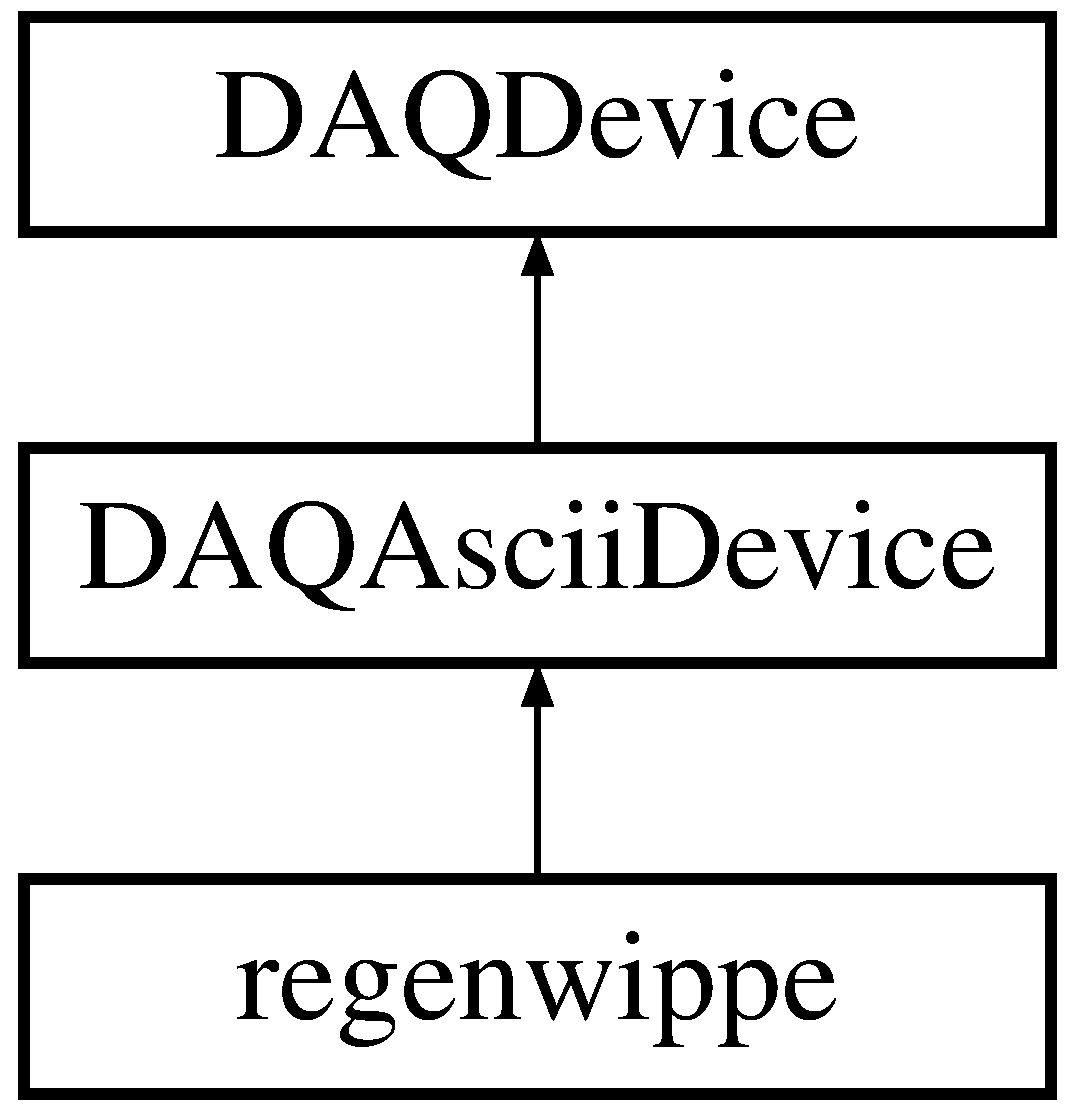
\includegraphics[height=3.000000cm]{classregenwippe}
\end{center}
\end{figure}
\subsection*{Public Member Functions}
\begin{DoxyCompactItemize}
\item 
\hyperlink{classregenwippe_a4ab9263a0e0e0f1d7d61386a8d172ee7}{regenwippe} ()
\item 
\hyperlink{classregenwippe_a73c61d128cec9d072d651829e49422c8}{$\sim$regenwippe} ()
\item 
void \hyperlink{classregenwippe_ac72996d1fc607aa1764a8838d1eeb943}{set\-Config\-Defaults} ()
\item 
int \hyperlink{classregenwippe_a349ee93b85dda804304b08d6244d2cf9}{read\-Header} (const char $\ast$\hyperlink{classDAQDevice_a7f9cda7cf5b41f6b134c313477e9644b}{filename})
\item 
int \hyperlink{classregenwippe_a0975a15b95532a6c3fb7be3dda8fd4e2}{parse\-Data} (char $\ast$line, struct timeval $\ast$l\-\_\-t\-Data, double $\ast$\hyperlink{classDAQDevice_ad148188c57598fdf4fd4c1c333aeb0d8}{sensor\-Value})
\item 
void \hyperlink{classregenwippe_a8229559506073be5033662daffe76243}{write\-Data} ()
\item 
unsigned int \hyperlink{classregenwippe_ad311e91cdfbd233971f51c9a635e47ba}{get\-Sensor\-Group} ()
\end{DoxyCompactItemize}
\subsection*{Private Attributes}
\begin{DoxyCompactItemize}
\item 
long \hyperlink{classregenwippe_aae07dc7dee8d390b563878aba636a047}{timestamp\-\_\-old}
\item 
int \hyperlink{classregenwippe_a36f67a6719525a1196e7ba2a3039c116}{sensor\-\_\-value\-\_\-old}
\item 
int \hyperlink{classregenwippe_ad36d8ccd489e7f1f9599bd7edac671c4}{n\-Show\-Data}
\end{DoxyCompactItemize}
\subsection*{Additional Inherited Members}


\subsection{Detailed Description}
Implementation for the weather mast D\-A\-Q devices that are used for turbulence, energy balance and 20m mast. 

\subsection{Constructor \& Destructor Documentation}
\hypertarget{classregenwippe_a4ab9263a0e0e0f1d7d61386a8d172ee7}{\index{regenwippe@{regenwippe}!regenwippe@{regenwippe}}
\index{regenwippe@{regenwippe}!regenwippe@{regenwippe}}
\subsubsection[{regenwippe}]{\setlength{\rightskip}{0pt plus 5cm}regenwippe\-::regenwippe (
\begin{DoxyParamCaption}
{}
\end{DoxyParamCaption}
)}}\label{classregenwippe_a4ab9263a0e0e0f1d7d61386a8d172ee7}
\hypertarget{classregenwippe_a73c61d128cec9d072d651829e49422c8}{\index{regenwippe@{regenwippe}!$\sim$regenwippe@{$\sim$regenwippe}}
\index{$\sim$regenwippe@{$\sim$regenwippe}!regenwippe@{regenwippe}}
\subsubsection[{$\sim$regenwippe}]{\setlength{\rightskip}{0pt plus 5cm}regenwippe\-::$\sim$regenwippe (
\begin{DoxyParamCaption}
{}
\end{DoxyParamCaption}
)}}\label{classregenwippe_a73c61d128cec9d072d651829e49422c8}


\subsection{Member Function Documentation}
\hypertarget{classregenwippe_ad311e91cdfbd233971f51c9a635e47ba}{\index{regenwippe@{regenwippe}!get\-Sensor\-Group@{get\-Sensor\-Group}}
\index{get\-Sensor\-Group@{get\-Sensor\-Group}!regenwippe@{regenwippe}}
\subsubsection[{get\-Sensor\-Group}]{\setlength{\rightskip}{0pt plus 5cm}unsigned int regenwippe\-::get\-Sensor\-Group (
\begin{DoxyParamCaption}
{}
\end{DoxyParamCaption}
)\hspace{0.3cm}{\ttfamily [virtual]}}}\label{classregenwippe_ad311e91cdfbd233971f51c9a635e47ba}
Define a sensor group number for all the availble sensor group files 

Reimplemented from \hyperlink{classDAQDevice_a61d08492a11c30944dfaf3b86115abe8}{D\-A\-Q\-Device}.

\hypertarget{classregenwippe_a0975a15b95532a6c3fb7be3dda8fd4e2}{\index{regenwippe@{regenwippe}!parse\-Data@{parse\-Data}}
\index{parse\-Data@{parse\-Data}!regenwippe@{regenwippe}}
\subsubsection[{parse\-Data}]{\setlength{\rightskip}{0pt plus 5cm}int regenwippe\-::parse\-Data (
\begin{DoxyParamCaption}
\item[{char $\ast$}]{line, }
\item[{struct timeval $\ast$}]{l\-\_\-t\-Data, }
\item[{double $\ast$}]{sensor\-Value}
\end{DoxyParamCaption}
)\hspace{0.3cm}{\ttfamily [virtual]}}}\label{classregenwippe_a0975a15b95532a6c3fb7be3dda8fd4e2}
Read the data from the current line of the data file. \begin{DoxyReturn}{Returns}
-\/1 no data found, skip storage 0 sucess, store data, 1 read another line 
\end{DoxyReturn}


Reimplemented from \hyperlink{classDAQAsciiDevice_a9c20d9d69af4ba1641dbc82dd5be2aa5}{D\-A\-Q\-Ascii\-Device}.

\hypertarget{classregenwippe_a349ee93b85dda804304b08d6244d2cf9}{\index{regenwippe@{regenwippe}!read\-Header@{read\-Header}}
\index{read\-Header@{read\-Header}!regenwippe@{regenwippe}}
\subsubsection[{read\-Header}]{\setlength{\rightskip}{0pt plus 5cm}int regenwippe\-::read\-Header (
\begin{DoxyParamCaption}
\item[{const char $\ast$}]{header}
\end{DoxyParamCaption}
)\hspace{0.3cm}{\ttfamily [virtual]}}}\label{classregenwippe_a349ee93b85dda804304b08d6244d2cf9}
Get time until next sample and it's id 

Reimplemented from \hyperlink{classDAQAsciiDevice_a5fce725c52b70ef2f56a34b32a03e15d}{D\-A\-Q\-Ascii\-Device}.

\hypertarget{classregenwippe_ac72996d1fc607aa1764a8838d1eeb943}{\index{regenwippe@{regenwippe}!set\-Config\-Defaults@{set\-Config\-Defaults}}
\index{set\-Config\-Defaults@{set\-Config\-Defaults}!regenwippe@{regenwippe}}
\subsubsection[{set\-Config\-Defaults}]{\setlength{\rightskip}{0pt plus 5cm}void regenwippe\-::set\-Config\-Defaults (
\begin{DoxyParamCaption}
{}
\end{DoxyParamCaption}
)\hspace{0.3cm}{\ttfamily [virtual]}}}\label{classregenwippe_ac72996d1fc607aa1764a8838d1eeb943}
The function is called before reading the configuration from the inifile. Use this fucntion in the module specific implementation to override the standard defaults 

Reimplemented from \hyperlink{classDAQDevice_a7685cec80865752cc0ef3ab49c6c2277}{D\-A\-Q\-Device}.

\hypertarget{classregenwippe_a8229559506073be5033662daffe76243}{\index{regenwippe@{regenwippe}!write\-Data@{write\-Data}}
\index{write\-Data@{write\-Data}!regenwippe@{regenwippe}}
\subsubsection[{write\-Data}]{\setlength{\rightskip}{0pt plus 5cm}void regenwippe\-::write\-Data (
\begin{DoxyParamCaption}
{}
\end{DoxyParamCaption}
)\hspace{0.3cm}{\ttfamily [virtual]}}}\label{classregenwippe_a8229559506073be5033662daffe76243}


Reimplemented from \hyperlink{classDAQDevice_acdc9d3765b1dfd845f99ec9c93071811}{D\-A\-Q\-Device}.



\subsection{Member Data Documentation}
\hypertarget{classregenwippe_ad36d8ccd489e7f1f9599bd7edac671c4}{\index{regenwippe@{regenwippe}!n\-Show\-Data@{n\-Show\-Data}}
\index{n\-Show\-Data@{n\-Show\-Data}!regenwippe@{regenwippe}}
\subsubsection[{n\-Show\-Data}]{\setlength{\rightskip}{0pt plus 5cm}int regenwippe\-::n\-Show\-Data\hspace{0.3cm}{\ttfamily [private]}}}\label{classregenwippe_ad36d8ccd489e7f1f9599bd7edac671c4}
Counter for lines to show after unclear data \hypertarget{classregenwippe_a36f67a6719525a1196e7ba2a3039c116}{\index{regenwippe@{regenwippe}!sensor\-\_\-value\-\_\-old@{sensor\-\_\-value\-\_\-old}}
\index{sensor\-\_\-value\-\_\-old@{sensor\-\_\-value\-\_\-old}!regenwippe@{regenwippe}}
\subsubsection[{sensor\-\_\-value\-\_\-old}]{\setlength{\rightskip}{0pt plus 5cm}int regenwippe\-::sensor\-\_\-value\-\_\-old\hspace{0.3cm}{\ttfamily [private]}}}\label{classregenwippe_a36f67a6719525a1196e7ba2a3039c116}
Last sensor data \hypertarget{classregenwippe_aae07dc7dee8d390b563878aba636a047}{\index{regenwippe@{regenwippe}!timestamp\-\_\-old@{timestamp\-\_\-old}}
\index{timestamp\-\_\-old@{timestamp\-\_\-old}!regenwippe@{regenwippe}}
\subsubsection[{timestamp\-\_\-old}]{\setlength{\rightskip}{0pt plus 5cm}long regenwippe\-::timestamp\-\_\-old\hspace{0.3cm}{\ttfamily [private]}}}\label{classregenwippe_aae07dc7dee8d390b563878aba636a047}
Last timestamp 

The documentation for this class was generated from the following files\-:\begin{DoxyCompactItemize}
\item 
/home/ntj/\-Development/phd/kitcube-\/tools/src/kitcube-\/devices/\hyperlink{regenwippe_8h}{regenwippe.\-h}\item 
/home/ntj/\-Development/phd/kitcube-\/tools/src/kitcube-\/devices/\hyperlink{regenwippe_8cpp}{regenwippe.\-cpp}\end{DoxyCompactItemize}

\hypertarget{structScanInfo}{\section{Scan\-Info Struct Reference}
\label{structScanInfo}\index{Scan\-Info@{Scan\-Info}}
}


{\ttfamily \#include $<$windtracer.\-h$>$}

\subsection*{Public Attributes}
\begin{DoxyCompactItemize}
\item 
struct \hyperlink{structBlockDescriptor}{Block\-Descriptor} \hyperlink{structScanInfo_aa35e33646202e65820e4e5877bb4638a}{block\-\_\-desc}
\item 
float \hyperlink{structScanInfo_a98d65e9d50d3fc3c382c8c30107829df}{f\-Scan\-Azimuth\-\_\-deg}
\item 
float \hyperlink{structScanInfo_af32649e9efdecf231eda758aac971ec3}{f\-Scan\-Elevation\-\_\-deg}
\item 
float \hyperlink{structScanInfo_abe3ee38419275b220a4f25bcfc86eac6}{f\-Azimuth\-Rate\-\_\-dps}
\item 
float \hyperlink{structScanInfo_aaa3e0950a443caa4c6d7ad54657edb5e}{f\-Elevation\-Rate\-\_\-dps}
\item 
float \hyperlink{structScanInfo_aad92fd2f9bbfd1fe8c8e682966cd5236}{f\-Target\-Azimuth\-\_\-deg}
\item 
float \hyperlink{structScanInfo_a26542bea822986447d7f7aba1ec52c1c}{f\-Target\-Elevation\-\_\-deg}
\item 
int32\-\_\-t \hyperlink{structScanInfo_a633fd4a80d1be23089f0447b24fec5d6}{n\-Scan\-Enabled}
\item 
int32\-\_\-t \hyperlink{structScanInfo_a79c26990e78094ff955e9f7bdc8af846}{n\-Current\-Index}
\item 
int32\-\_\-t \hyperlink{structScanInfo_aa96fd85db33fb38d6f8a2dec1e124333}{n\-Acq\-Scan\-State}
\item 
int32\-\_\-t \hyperlink{structScanInfo_a7cd377a6edb4dfb4ff79d77ee9638bda}{n\-Driver\-Scan\-State}
\item 
int32\-\_\-t \hyperlink{structScanInfo_abef44f09d1d490fa380edff9a6d7e501}{n\-Acq\-Dwell\-State}
\item 
int32\-\_\-t \hyperlink{structScanInfo_a3734fd5525b106f219a16d77440170e4}{n\-Scan\-Pattern\-Type}
\item 
u\-\_\-int32\-\_\-t \hyperlink{structScanInfo_a297a9e4889f6caaffba6d3b9c1a9d1dc}{n\-Valid\-Pos}
\item 
int32\-\_\-t \hyperlink{structScanInfo_a4ad5cbb492f1e6042a54c9c2ea3a48be}{n\-S\-S\-Done\-State}
\item 
u\-\_\-int32\-\_\-t \hyperlink{structScanInfo_a9d77d5adef2042b142b23186dcb0635f}{n\-Error\-Flags}
\end{DoxyCompactItemize}


\subsection{Member Data Documentation}
\hypertarget{structScanInfo_aa35e33646202e65820e4e5877bb4638a}{\index{Scan\-Info@{Scan\-Info}!block\-\_\-desc@{block\-\_\-desc}}
\index{block\-\_\-desc@{block\-\_\-desc}!ScanInfo@{Scan\-Info}}
\subsubsection[{block\-\_\-desc}]{\setlength{\rightskip}{0pt plus 5cm}struct {\bf Block\-Descriptor} Scan\-Info\-::block\-\_\-desc}}\label{structScanInfo_aa35e33646202e65820e4e5877bb4638a}
\hypertarget{structScanInfo_abe3ee38419275b220a4f25bcfc86eac6}{\index{Scan\-Info@{Scan\-Info}!f\-Azimuth\-Rate\-\_\-dps@{f\-Azimuth\-Rate\-\_\-dps}}
\index{f\-Azimuth\-Rate\-\_\-dps@{f\-Azimuth\-Rate\-\_\-dps}!ScanInfo@{Scan\-Info}}
\subsubsection[{f\-Azimuth\-Rate\-\_\-dps}]{\setlength{\rightskip}{0pt plus 5cm}float Scan\-Info\-::f\-Azimuth\-Rate\-\_\-dps}}\label{structScanInfo_abe3ee38419275b220a4f25bcfc86eac6}
\hypertarget{structScanInfo_aaa3e0950a443caa4c6d7ad54657edb5e}{\index{Scan\-Info@{Scan\-Info}!f\-Elevation\-Rate\-\_\-dps@{f\-Elevation\-Rate\-\_\-dps}}
\index{f\-Elevation\-Rate\-\_\-dps@{f\-Elevation\-Rate\-\_\-dps}!ScanInfo@{Scan\-Info}}
\subsubsection[{f\-Elevation\-Rate\-\_\-dps}]{\setlength{\rightskip}{0pt plus 5cm}float Scan\-Info\-::f\-Elevation\-Rate\-\_\-dps}}\label{structScanInfo_aaa3e0950a443caa4c6d7ad54657edb5e}
\hypertarget{structScanInfo_a98d65e9d50d3fc3c382c8c30107829df}{\index{Scan\-Info@{Scan\-Info}!f\-Scan\-Azimuth\-\_\-deg@{f\-Scan\-Azimuth\-\_\-deg}}
\index{f\-Scan\-Azimuth\-\_\-deg@{f\-Scan\-Azimuth\-\_\-deg}!ScanInfo@{Scan\-Info}}
\subsubsection[{f\-Scan\-Azimuth\-\_\-deg}]{\setlength{\rightskip}{0pt plus 5cm}float Scan\-Info\-::f\-Scan\-Azimuth\-\_\-deg}}\label{structScanInfo_a98d65e9d50d3fc3c382c8c30107829df}
\hypertarget{structScanInfo_af32649e9efdecf231eda758aac971ec3}{\index{Scan\-Info@{Scan\-Info}!f\-Scan\-Elevation\-\_\-deg@{f\-Scan\-Elevation\-\_\-deg}}
\index{f\-Scan\-Elevation\-\_\-deg@{f\-Scan\-Elevation\-\_\-deg}!ScanInfo@{Scan\-Info}}
\subsubsection[{f\-Scan\-Elevation\-\_\-deg}]{\setlength{\rightskip}{0pt plus 5cm}float Scan\-Info\-::f\-Scan\-Elevation\-\_\-deg}}\label{structScanInfo_af32649e9efdecf231eda758aac971ec3}
\hypertarget{structScanInfo_aad92fd2f9bbfd1fe8c8e682966cd5236}{\index{Scan\-Info@{Scan\-Info}!f\-Target\-Azimuth\-\_\-deg@{f\-Target\-Azimuth\-\_\-deg}}
\index{f\-Target\-Azimuth\-\_\-deg@{f\-Target\-Azimuth\-\_\-deg}!ScanInfo@{Scan\-Info}}
\subsubsection[{f\-Target\-Azimuth\-\_\-deg}]{\setlength{\rightskip}{0pt plus 5cm}float Scan\-Info\-::f\-Target\-Azimuth\-\_\-deg}}\label{structScanInfo_aad92fd2f9bbfd1fe8c8e682966cd5236}
\hypertarget{structScanInfo_a26542bea822986447d7f7aba1ec52c1c}{\index{Scan\-Info@{Scan\-Info}!f\-Target\-Elevation\-\_\-deg@{f\-Target\-Elevation\-\_\-deg}}
\index{f\-Target\-Elevation\-\_\-deg@{f\-Target\-Elevation\-\_\-deg}!ScanInfo@{Scan\-Info}}
\subsubsection[{f\-Target\-Elevation\-\_\-deg}]{\setlength{\rightskip}{0pt plus 5cm}float Scan\-Info\-::f\-Target\-Elevation\-\_\-deg}}\label{structScanInfo_a26542bea822986447d7f7aba1ec52c1c}
\hypertarget{structScanInfo_abef44f09d1d490fa380edff9a6d7e501}{\index{Scan\-Info@{Scan\-Info}!n\-Acq\-Dwell\-State@{n\-Acq\-Dwell\-State}}
\index{n\-Acq\-Dwell\-State@{n\-Acq\-Dwell\-State}!ScanInfo@{Scan\-Info}}
\subsubsection[{n\-Acq\-Dwell\-State}]{\setlength{\rightskip}{0pt plus 5cm}int32\-\_\-t Scan\-Info\-::n\-Acq\-Dwell\-State}}\label{structScanInfo_abef44f09d1d490fa380edff9a6d7e501}
\hypertarget{structScanInfo_aa96fd85db33fb38d6f8a2dec1e124333}{\index{Scan\-Info@{Scan\-Info}!n\-Acq\-Scan\-State@{n\-Acq\-Scan\-State}}
\index{n\-Acq\-Scan\-State@{n\-Acq\-Scan\-State}!ScanInfo@{Scan\-Info}}
\subsubsection[{n\-Acq\-Scan\-State}]{\setlength{\rightskip}{0pt plus 5cm}int32\-\_\-t Scan\-Info\-::n\-Acq\-Scan\-State}}\label{structScanInfo_aa96fd85db33fb38d6f8a2dec1e124333}
\hypertarget{structScanInfo_a79c26990e78094ff955e9f7bdc8af846}{\index{Scan\-Info@{Scan\-Info}!n\-Current\-Index@{n\-Current\-Index}}
\index{n\-Current\-Index@{n\-Current\-Index}!ScanInfo@{Scan\-Info}}
\subsubsection[{n\-Current\-Index}]{\setlength{\rightskip}{0pt plus 5cm}int32\-\_\-t Scan\-Info\-::n\-Current\-Index}}\label{structScanInfo_a79c26990e78094ff955e9f7bdc8af846}
\hypertarget{structScanInfo_a7cd377a6edb4dfb4ff79d77ee9638bda}{\index{Scan\-Info@{Scan\-Info}!n\-Driver\-Scan\-State@{n\-Driver\-Scan\-State}}
\index{n\-Driver\-Scan\-State@{n\-Driver\-Scan\-State}!ScanInfo@{Scan\-Info}}
\subsubsection[{n\-Driver\-Scan\-State}]{\setlength{\rightskip}{0pt plus 5cm}int32\-\_\-t Scan\-Info\-::n\-Driver\-Scan\-State}}\label{structScanInfo_a7cd377a6edb4dfb4ff79d77ee9638bda}
\hypertarget{structScanInfo_a9d77d5adef2042b142b23186dcb0635f}{\index{Scan\-Info@{Scan\-Info}!n\-Error\-Flags@{n\-Error\-Flags}}
\index{n\-Error\-Flags@{n\-Error\-Flags}!ScanInfo@{Scan\-Info}}
\subsubsection[{n\-Error\-Flags}]{\setlength{\rightskip}{0pt plus 5cm}u\-\_\-int32\-\_\-t Scan\-Info\-::n\-Error\-Flags}}\label{structScanInfo_a9d77d5adef2042b142b23186dcb0635f}
\hypertarget{structScanInfo_a633fd4a80d1be23089f0447b24fec5d6}{\index{Scan\-Info@{Scan\-Info}!n\-Scan\-Enabled@{n\-Scan\-Enabled}}
\index{n\-Scan\-Enabled@{n\-Scan\-Enabled}!ScanInfo@{Scan\-Info}}
\subsubsection[{n\-Scan\-Enabled}]{\setlength{\rightskip}{0pt plus 5cm}int32\-\_\-t Scan\-Info\-::n\-Scan\-Enabled}}\label{structScanInfo_a633fd4a80d1be23089f0447b24fec5d6}
\hypertarget{structScanInfo_a3734fd5525b106f219a16d77440170e4}{\index{Scan\-Info@{Scan\-Info}!n\-Scan\-Pattern\-Type@{n\-Scan\-Pattern\-Type}}
\index{n\-Scan\-Pattern\-Type@{n\-Scan\-Pattern\-Type}!ScanInfo@{Scan\-Info}}
\subsubsection[{n\-Scan\-Pattern\-Type}]{\setlength{\rightskip}{0pt plus 5cm}int32\-\_\-t Scan\-Info\-::n\-Scan\-Pattern\-Type}}\label{structScanInfo_a3734fd5525b106f219a16d77440170e4}
\hypertarget{structScanInfo_a4ad5cbb492f1e6042a54c9c2ea3a48be}{\index{Scan\-Info@{Scan\-Info}!n\-S\-S\-Done\-State@{n\-S\-S\-Done\-State}}
\index{n\-S\-S\-Done\-State@{n\-S\-S\-Done\-State}!ScanInfo@{Scan\-Info}}
\subsubsection[{n\-S\-S\-Done\-State}]{\setlength{\rightskip}{0pt plus 5cm}int32\-\_\-t Scan\-Info\-::n\-S\-S\-Done\-State}}\label{structScanInfo_a4ad5cbb492f1e6042a54c9c2ea3a48be}
\hypertarget{structScanInfo_a297a9e4889f6caaffba6d3b9c1a9d1dc}{\index{Scan\-Info@{Scan\-Info}!n\-Valid\-Pos@{n\-Valid\-Pos}}
\index{n\-Valid\-Pos@{n\-Valid\-Pos}!ScanInfo@{Scan\-Info}}
\subsubsection[{n\-Valid\-Pos}]{\setlength{\rightskip}{0pt plus 5cm}u\-\_\-int32\-\_\-t Scan\-Info\-::n\-Valid\-Pos}}\label{structScanInfo_a297a9e4889f6caaffba6d3b9c1a9d1dc}


The documentation for this struct was generated from the following file\-:\begin{DoxyCompactItemize}
\item 
/home/ntj/\-Development/phd/kitcube-\/tools/src/kitcube-\/devices/\hyperlink{windtracer_8h}{windtracer.\-h}\end{DoxyCompactItemize}

\hypertarget{classsci}{\section{sci Class Reference}
\label{classsci}\index{sci@{sci}}
}


{\ttfamily \#include $<$scintillometer.\-h$>$}

Inheritance diagram for sci\-:\begin{figure}[H]
\begin{center}
\leavevmode
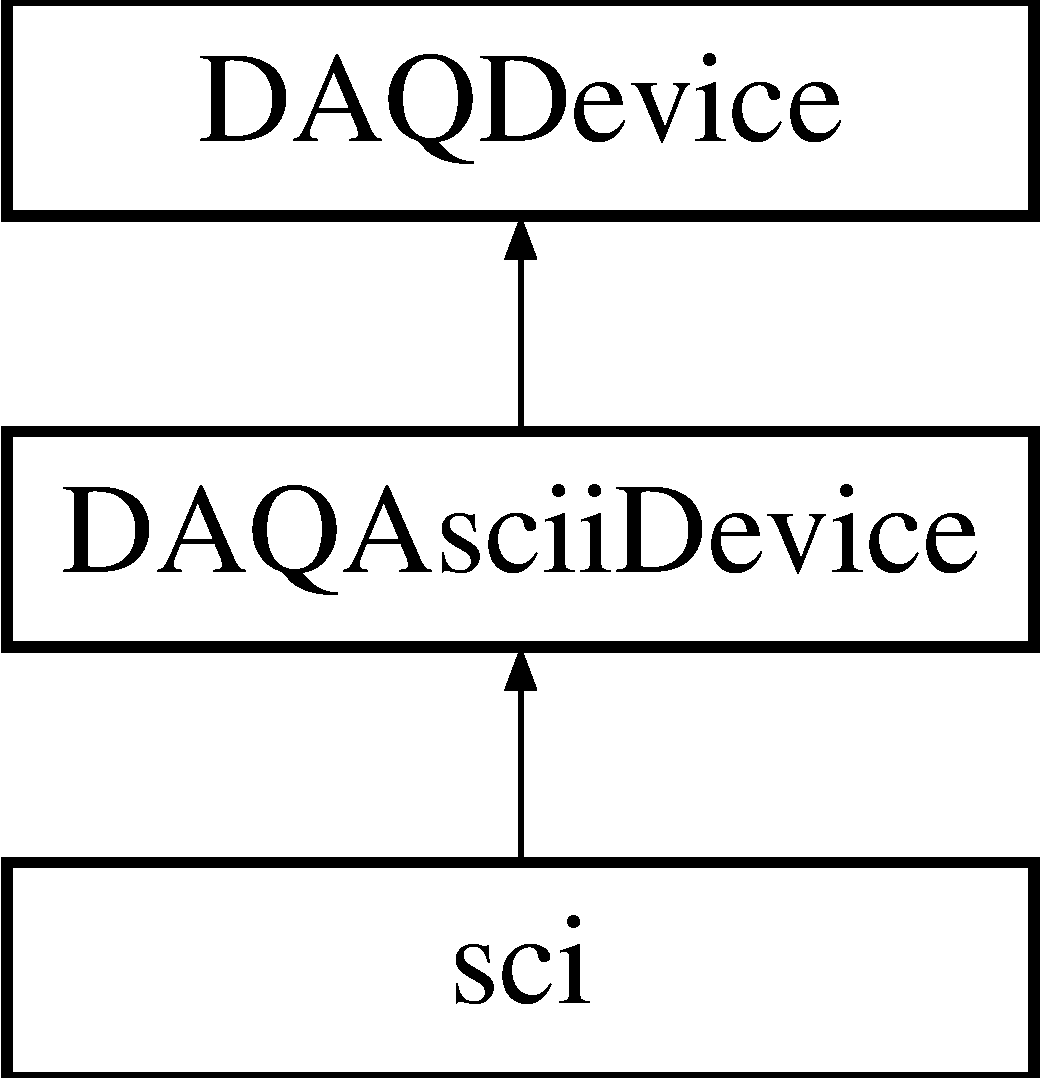
\includegraphics[height=3.000000cm]{classsci}
\end{center}
\end{figure}
\subsection*{Public Member Functions}
\begin{DoxyCompactItemize}
\item 
\hyperlink{classsci_a174afce65f9b9189f2deab5b03538065}{sci} ()
\item 
\hyperlink{classsci_a38001383ffb08170088809b0b271f3f7}{$\sim$sci} ()
\item 
void \hyperlink{classsci_a0f0a2b8d161af6f539e202ff5357c56f}{set\-Config\-Defaults} ()
\item 
int \hyperlink{classsci_acf9c29e3fe47d89795dd4160525c008f}{read\-Header} (const char $\ast$\hyperlink{classDAQDevice_a7f9cda7cf5b41f6b134c313477e9644b}{filename})
\item 
int \hyperlink{classsci_abb8bd3f6f3861a95e4977614fd9cea70}{parse\-Data} (char $\ast$line, struct timeval $\ast$l\-\_\-t\-Data, double $\ast$\hyperlink{classDAQDevice_ad148188c57598fdf4fd4c1c333aeb0d8}{sensor\-Value})
\item 
unsigned int \hyperlink{classsci_a54872e325b018dabbd6f60e0443f864c}{get\-Sensor\-Group} ()
\end{DoxyCompactItemize}
\subsection*{Additional Inherited Members}


\subsection{Detailed Description}
Implementation for the scintillometer 

\subsection{Constructor \& Destructor Documentation}
\hypertarget{classsci_a174afce65f9b9189f2deab5b03538065}{\index{sci@{sci}!sci@{sci}}
\index{sci@{sci}!sci@{sci}}
\subsubsection[{sci}]{\setlength{\rightskip}{0pt plus 5cm}sci\-::sci (
\begin{DoxyParamCaption}
{}
\end{DoxyParamCaption}
)}}\label{classsci_a174afce65f9b9189f2deab5b03538065}
\hypertarget{classsci_a38001383ffb08170088809b0b271f3f7}{\index{sci@{sci}!$\sim$sci@{$\sim$sci}}
\index{$\sim$sci@{$\sim$sci}!sci@{sci}}
\subsubsection[{$\sim$sci}]{\setlength{\rightskip}{0pt plus 5cm}sci\-::$\sim$sci (
\begin{DoxyParamCaption}
{}
\end{DoxyParamCaption}
)}}\label{classsci_a38001383ffb08170088809b0b271f3f7}


\subsection{Member Function Documentation}
\hypertarget{classsci_a54872e325b018dabbd6f60e0443f864c}{\index{sci@{sci}!get\-Sensor\-Group@{get\-Sensor\-Group}}
\index{get\-Sensor\-Group@{get\-Sensor\-Group}!sci@{sci}}
\subsubsection[{get\-Sensor\-Group}]{\setlength{\rightskip}{0pt plus 5cm}unsigned int sci\-::get\-Sensor\-Group (
\begin{DoxyParamCaption}
{}
\end{DoxyParamCaption}
)\hspace{0.3cm}{\ttfamily [virtual]}}}\label{classsci_a54872e325b018dabbd6f60e0443f864c}
Define a sensor group number for all the availble sensor group files 

Reimplemented from \hyperlink{classDAQDevice_a61d08492a11c30944dfaf3b86115abe8}{D\-A\-Q\-Device}.

\hypertarget{classsci_abb8bd3f6f3861a95e4977614fd9cea70}{\index{sci@{sci}!parse\-Data@{parse\-Data}}
\index{parse\-Data@{parse\-Data}!sci@{sci}}
\subsubsection[{parse\-Data}]{\setlength{\rightskip}{0pt plus 5cm}int sci\-::parse\-Data (
\begin{DoxyParamCaption}
\item[{char $\ast$}]{line, }
\item[{struct timeval $\ast$}]{l\-\_\-t\-Data, }
\item[{double $\ast$}]{sensor\-Value}
\end{DoxyParamCaption}
)\hspace{0.3cm}{\ttfamily [virtual]}}}\label{classsci_abb8bd3f6f3861a95e4977614fd9cea70}
Read the data from the current line of the data file. \begin{DoxyReturn}{Returns}
-\/1 no data found, skip storage 0 sucess, store data, 1 read another line 
\end{DoxyReturn}


Reimplemented from \hyperlink{classDAQAsciiDevice_a9c20d9d69af4ba1641dbc82dd5be2aa5}{D\-A\-Q\-Ascii\-Device}.

\hypertarget{classsci_acf9c29e3fe47d89795dd4160525c008f}{\index{sci@{sci}!read\-Header@{read\-Header}}
\index{read\-Header@{read\-Header}!sci@{sci}}
\subsubsection[{read\-Header}]{\setlength{\rightskip}{0pt plus 5cm}int sci\-::read\-Header (
\begin{DoxyParamCaption}
\item[{const char $\ast$}]{header}
\end{DoxyParamCaption}
)\hspace{0.3cm}{\ttfamily [virtual]}}}\label{classsci_acf9c29e3fe47d89795dd4160525c008f}
Get time until next sample and it's id 

Reimplemented from \hyperlink{classDAQAsciiDevice_a5fce725c52b70ef2f56a34b32a03e15d}{D\-A\-Q\-Ascii\-Device}.

\hypertarget{classsci_a0f0a2b8d161af6f539e202ff5357c56f}{\index{sci@{sci}!set\-Config\-Defaults@{set\-Config\-Defaults}}
\index{set\-Config\-Defaults@{set\-Config\-Defaults}!sci@{sci}}
\subsubsection[{set\-Config\-Defaults}]{\setlength{\rightskip}{0pt plus 5cm}void sci\-::set\-Config\-Defaults (
\begin{DoxyParamCaption}
{}
\end{DoxyParamCaption}
)\hspace{0.3cm}{\ttfamily [virtual]}}}\label{classsci_a0f0a2b8d161af6f539e202ff5357c56f}
The function is called before reading the configuration from the inifile. Use this fucntion in the module specific implementation to override the standard defaults 

Reimplemented from \hyperlink{classDAQDevice_a7685cec80865752cc0ef3ab49c6c2277}{D\-A\-Q\-Device}.



The documentation for this class was generated from the following files\-:\begin{DoxyCompactItemize}
\item 
/home/ntj/\-Development/phd/kitcube-\/tools/src/kitcube-\/devices/\hyperlink{scintillometer_8h}{scintillometer.\-h}\item 
/home/ntj/\-Development/phd/kitcube-\/tools/src/kitcube-\/devices/\hyperlink{scintillometer_8cpp}{scintillometer.\-cpp}\end{DoxyCompactItemize}

\hypertarget{classsemaphore}{\section{semaphore Class Reference}
\label{classsemaphore}\index{semaphore@{semaphore}}
}


{\ttfamily \#include $<$semaphore.\-h$>$}

\subsection*{Public Member Functions}
\begin{DoxyCompactItemize}
\item 
\hyperlink{classsemaphore_a31507ed70a3da29a101b37c5cb9e286e}{semaphore} (int mid=0, const char $\ast$dir=\char`\"{}/\char`\"{})
\item 
void \hyperlink{classsemaphore_a7fabe8758afc2f2b3f62c45514ab1b6a}{request} (int nr=0)
\item 
void \hyperlink{classsemaphore_a1979f4ba3834a6e12fd32ceca4e9d261}{release} (int nr=0)
\item 
int \hyperlink{classsemaphore_a2e79d2e0e2ce47d698f51ecc91b76b39}{number} ()
\end{DoxyCompactItemize}
\subsection*{Private Attributes}
\begin{DoxyCompactItemize}
\item 
int \hyperlink{classsemaphore_a64fc11fb8a84ceb95e510829795ed996}{memid}
\end{DoxyCompactItemize}


\subsection{Detailed Description}
\begin{DoxyVerb}The class provides semaphores.
With Linux the SysV style semaphores are used.

The function of the semaphores is crucial to all applications
relying on Pbus-access. To maintain the state of the semaphores
use the program "semtool" or the system commands "ipcs" and "ipcrm".

List the state of the semphores.
\end{DoxyVerb}
 \begin{DoxyVerb}semtool t\end{DoxyVerb}
 \begin{DoxyVerb}After an abnormal program end it can happen, that semapohres stay
locked. Any access to the electronic will be impossible in this state.
Use "semtool" to clear the state of the semaphores.
\end{DoxyVerb}
 \begin{DoxyVerb}\end{DoxyVerb}


\begin{DoxyRefDesc}{Todo}
\item[\hyperlink{todo__todo000004}{Todo}]Would be nice to have named semaphores with a automatic numbering?! 

There is another definition of semaphores in \hyperlink{semaphore_8h}{semaphore.\-h}. Is this useful? 

G\-U\-I programm for Windows N\-T also need protection, when multiple threads are used! Try to adapt a version with the M\-F\-C Semaphores.\end{DoxyRefDesc}


\begin{DoxyRefDesc}{Todo}
\item[\hyperlink{todo__todo000005}{Todo}]Add optional argument to the constructor to define a message stream.\end{DoxyRefDesc}


\subsection{Constructor \& Destructor Documentation}
\hypertarget{classsemaphore_a31507ed70a3da29a101b37c5cb9e286e}{\index{semaphore@{semaphore}!semaphore@{semaphore}}
\index{semaphore@{semaphore}!semaphore@{semaphore}}
\subsubsection[{semaphore}]{\setlength{\rightskip}{0pt plus 5cm}semaphore\-::semaphore (
\begin{DoxyParamCaption}
\item[{int}]{mid = {\ttfamily 0}, }
\item[{const char $\ast$}]{dir = {\ttfamily \char`\"{}/\char`\"{}}}
\end{DoxyParamCaption}
)}}\label{classsemaphore_a31507ed70a3da29a101b37c5cb9e286e}
Creates a Semaphore array. 
\begin{DoxyParams}{Parameters}
{\em mid} & Number of the (first) Semaphore in the array \\
\hline
{\em dir} & Name of the base directory \\
\hline
\end{DoxyParams}


\subsection{Member Function Documentation}
\hypertarget{classsemaphore_a2e79d2e0e2ce47d698f51ecc91b76b39}{\index{semaphore@{semaphore}!number@{number}}
\index{number@{number}!semaphore@{semaphore}}
\subsubsection[{number}]{\setlength{\rightskip}{0pt plus 5cm}int semaphore\-::number (
\begin{DoxyParamCaption}
{}
\end{DoxyParamCaption}
)}}\label{classsemaphore_a2e79d2e0e2ce47d698f51ecc91b76b39}
Returns the number of semaphores in the array \hypertarget{classsemaphore_a1979f4ba3834a6e12fd32ceca4e9d261}{\index{semaphore@{semaphore}!release@{release}}
\index{release@{release}!semaphore@{semaphore}}
\subsubsection[{release}]{\setlength{\rightskip}{0pt plus 5cm}void semaphore\-::release (
\begin{DoxyParamCaption}
\item[{int}]{nr = {\ttfamily 0}}
\end{DoxyParamCaption}
)}}\label{classsemaphore_a1979f4ba3834a6e12fd32ceca4e9d261}
\hypertarget{classsemaphore_a7fabe8758afc2f2b3f62c45514ab1b6a}{\index{semaphore@{semaphore}!request@{request}}
\index{request@{request}!semaphore@{semaphore}}
\subsubsection[{request}]{\setlength{\rightskip}{0pt plus 5cm}void semaphore\-::request (
\begin{DoxyParamCaption}
\item[{int}]{nr = {\ttfamily 0}}
\end{DoxyParamCaption}
)}}\label{classsemaphore_a7fabe8758afc2f2b3f62c45514ab1b6a}


\subsection{Member Data Documentation}
\hypertarget{classsemaphore_a64fc11fb8a84ceb95e510829795ed996}{\index{semaphore@{semaphore}!memid@{memid}}
\index{memid@{memid}!semaphore@{semaphore}}
\subsubsection[{memid}]{\setlength{\rightskip}{0pt plus 5cm}int semaphore\-::memid\hspace{0.3cm}{\ttfamily [private]}}}\label{classsemaphore_a64fc11fb8a84ceb95e510829795ed996}
Returns the key of the semphore array This is the number that can be found in the display of the system command \char`\"{}ipcs\char`\"{}. 

The documentation for this class was generated from the following files\-:\begin{DoxyCompactItemize}
\item 
/home/ntj/\-Development/phd/kitcube-\/tools/src/akutil/\hyperlink{semaphore_8h}{semaphore.\-h}\item 
/home/ntj/\-Development/phd/kitcube-\/tools/src/akutil/\hyperlink{semaphore_8cpp}{semaphore.\-cpp}\end{DoxyCompactItemize}

\hypertarget{structsensorType}{\section{sensor\-Type Struct Reference}
\label{structsensorType}\index{sensor\-Type@{sensor\-Type}}
}


{\ttfamily \#include $<$daqdevice.\-h$>$}

\subsection*{Public Attributes}
\begin{DoxyCompactItemize}
\item 
std\-::string \hyperlink{structsensorType_a839167cca6fe6ccd714bc106024ef05b}{name}
\item 
std\-::string \hyperlink{structsensorType_a81883599e96d5ad052203a3d46288187}{comment}
\item 
std\-::string \hyperlink{structsensorType_af7949131476e3d41809a66e56a19dd37}{long\-Comment}
\item 
std\-::string \hyperlink{structsensorType_aa79c2e4762be819e51b68fabed355c70}{unit}
\item 
std\-::string \hyperlink{structsensorType_a8e29e9b36a7bffe8ed80b4760266fa70}{type}
\item 
int \hyperlink{structsensorType_aaf364b2726c24b2f1e8555f12affe945}{aggregation}
\item 
int \hyperlink{structsensorType_af6bb097492d08aba292d4fd3fe26bc72}{axis}
\item 
std\-::string \hyperlink{structsensorType_a9c0494226b832c301af8a1a0a93b435a}{axis2\-\_\-name}
\item 
int \hyperlink{structsensorType_ae789d72cd0530bc886972463d6ff0ad5}{axis2}
\item 
int \hyperlink{structsensorType_a4beadcfed6e0266de2a8cfa21765e491}{axis2\-\_\-idx}
\item 
float \hyperlink{structsensorType_af861068c9850daaa347b0320daf38bc9}{axis2\-\_\-val}
\item 
float \hyperlink{structsensorType_a585db9c20888c66022c8493d2177e480}{height}
\item 
std\-::string \hyperlink{structsensorType_adabebb37268ffe2dfdba8517f6e9a87d}{data\-\_\-format}
\item 
int \hyperlink{structsensorType_ac4e84f68987ad6ce6d8b1b1736ed2f44}{size}
\end{DoxyCompactItemize}


\subsection{Member Data Documentation}
\hypertarget{structsensorType_aaf364b2726c24b2f1e8555f12affe945}{\index{sensor\-Type@{sensor\-Type}!aggregation@{aggregation}}
\index{aggregation@{aggregation}!sensorType@{sensor\-Type}}
\subsubsection[{aggregation}]{\setlength{\rightskip}{0pt plus 5cm}int sensor\-Type\-::aggregation}}\label{structsensorType_aaf364b2726c24b2f1e8555f12affe945}
\hypertarget{structsensorType_af6bb097492d08aba292d4fd3fe26bc72}{\index{sensor\-Type@{sensor\-Type}!axis@{axis}}
\index{axis@{axis}!sensorType@{sensor\-Type}}
\subsubsection[{axis}]{\setlength{\rightskip}{0pt plus 5cm}int sensor\-Type\-::axis}}\label{structsensorType_af6bb097492d08aba292d4fd3fe26bc72}
\hypertarget{structsensorType_ae789d72cd0530bc886972463d6ff0ad5}{\index{sensor\-Type@{sensor\-Type}!axis2@{axis2}}
\index{axis2@{axis2}!sensorType@{sensor\-Type}}
\subsubsection[{axis2}]{\setlength{\rightskip}{0pt plus 5cm}int sensor\-Type\-::axis2}}\label{structsensorType_ae789d72cd0530bc886972463d6ff0ad5}
\hypertarget{structsensorType_a4beadcfed6e0266de2a8cfa21765e491}{\index{sensor\-Type@{sensor\-Type}!axis2\-\_\-idx@{axis2\-\_\-idx}}
\index{axis2\-\_\-idx@{axis2\-\_\-idx}!sensorType@{sensor\-Type}}
\subsubsection[{axis2\-\_\-idx}]{\setlength{\rightskip}{0pt plus 5cm}int sensor\-Type\-::axis2\-\_\-idx}}\label{structsensorType_a4beadcfed6e0266de2a8cfa21765e491}
\hypertarget{structsensorType_a9c0494226b832c301af8a1a0a93b435a}{\index{sensor\-Type@{sensor\-Type}!axis2\-\_\-name@{axis2\-\_\-name}}
\index{axis2\-\_\-name@{axis2\-\_\-name}!sensorType@{sensor\-Type}}
\subsubsection[{axis2\-\_\-name}]{\setlength{\rightskip}{0pt plus 5cm}std\-::string sensor\-Type\-::axis2\-\_\-name}}\label{structsensorType_a9c0494226b832c301af8a1a0a93b435a}
\hypertarget{structsensorType_af861068c9850daaa347b0320daf38bc9}{\index{sensor\-Type@{sensor\-Type}!axis2\-\_\-val@{axis2\-\_\-val}}
\index{axis2\-\_\-val@{axis2\-\_\-val}!sensorType@{sensor\-Type}}
\subsubsection[{axis2\-\_\-val}]{\setlength{\rightskip}{0pt plus 5cm}float sensor\-Type\-::axis2\-\_\-val}}\label{structsensorType_af861068c9850daaa347b0320daf38bc9}
\hypertarget{structsensorType_a81883599e96d5ad052203a3d46288187}{\index{sensor\-Type@{sensor\-Type}!comment@{comment}}
\index{comment@{comment}!sensorType@{sensor\-Type}}
\subsubsection[{comment}]{\setlength{\rightskip}{0pt plus 5cm}std\-::string sensor\-Type\-::comment}}\label{structsensorType_a81883599e96d5ad052203a3d46288187}
\hypertarget{structsensorType_adabebb37268ffe2dfdba8517f6e9a87d}{\index{sensor\-Type@{sensor\-Type}!data\-\_\-format@{data\-\_\-format}}
\index{data\-\_\-format@{data\-\_\-format}!sensorType@{sensor\-Type}}
\subsubsection[{data\-\_\-format}]{\setlength{\rightskip}{0pt plus 5cm}std\-::string sensor\-Type\-::data\-\_\-format}}\label{structsensorType_adabebb37268ffe2dfdba8517f6e9a87d}
\hypertarget{structsensorType_a585db9c20888c66022c8493d2177e480}{\index{sensor\-Type@{sensor\-Type}!height@{height}}
\index{height@{height}!sensorType@{sensor\-Type}}
\subsubsection[{height}]{\setlength{\rightskip}{0pt plus 5cm}float sensor\-Type\-::height}}\label{structsensorType_a585db9c20888c66022c8493d2177e480}
\hypertarget{structsensorType_af7949131476e3d41809a66e56a19dd37}{\index{sensor\-Type@{sensor\-Type}!long\-Comment@{long\-Comment}}
\index{long\-Comment@{long\-Comment}!sensorType@{sensor\-Type}}
\subsubsection[{long\-Comment}]{\setlength{\rightskip}{0pt plus 5cm}std\-::string sensor\-Type\-::long\-Comment}}\label{structsensorType_af7949131476e3d41809a66e56a19dd37}
\hypertarget{structsensorType_a839167cca6fe6ccd714bc106024ef05b}{\index{sensor\-Type@{sensor\-Type}!name@{name}}
\index{name@{name}!sensorType@{sensor\-Type}}
\subsubsection[{name}]{\setlength{\rightskip}{0pt plus 5cm}std\-::string sensor\-Type\-::name}}\label{structsensorType_a839167cca6fe6ccd714bc106024ef05b}
\hypertarget{structsensorType_ac4e84f68987ad6ce6d8b1b1736ed2f44}{\index{sensor\-Type@{sensor\-Type}!size@{size}}
\index{size@{size}!sensorType@{sensor\-Type}}
\subsubsection[{size}]{\setlength{\rightskip}{0pt plus 5cm}int sensor\-Type\-::size}}\label{structsensorType_ac4e84f68987ad6ce6d8b1b1736ed2f44}
\hypertarget{structsensorType_a8e29e9b36a7bffe8ed80b4760266fa70}{\index{sensor\-Type@{sensor\-Type}!type@{type}}
\index{type@{type}!sensorType@{sensor\-Type}}
\subsubsection[{type}]{\setlength{\rightskip}{0pt plus 5cm}std\-::string sensor\-Type\-::type}}\label{structsensorType_a8e29e9b36a7bffe8ed80b4760266fa70}
\hypertarget{structsensorType_aa79c2e4762be819e51b68fabed355c70}{\index{sensor\-Type@{sensor\-Type}!unit@{unit}}
\index{unit@{unit}!sensorType@{sensor\-Type}}
\subsubsection[{unit}]{\setlength{\rightskip}{0pt plus 5cm}std\-::string sensor\-Type\-::unit}}\label{structsensorType_aa79c2e4762be819e51b68fabed355c70}


The documentation for this struct was generated from the following file\-:\begin{DoxyCompactItemize}
\item 
/home/ntj/\-Development/phd/kitcube-\/tools/src/kitcube-\/devices/\hyperlink{daqdevice_8h}{daqdevice.\-h}\end{DoxyCompactItemize}

\hypertarget{classsharedMemory}{\section{shared\-Memory Class Reference}
\label{classsharedMemory}\index{shared\-Memory@{shared\-Memory}}
}


{\ttfamily \#include $<$shared\-Memory.\-h$>$}

\subsection*{Public Member Functions}
\begin{DoxyCompactItemize}
\item 
\hyperlink{classsharedMemory_ac45cb96bec31a5eb46108c0f203cb417}{shared\-Memory} (int size, const char $\ast$dir=\char`\"{}$\sim$\char`\"{})
\item 
char $\ast$ \hyperlink{classsharedMemory_aa45ce6ed2e7ca4d5a3ad1c25ecd6dc81}{get\-Reference} ()
\item 
void \hyperlink{classsharedMemory_ae83cb80fd537392f47bf62080a7239a6}{remove} ()
\item 
int \hyperlink{classsharedMemory_a2b067bb02ea5175c760b4a75514500f9}{get\-Size} ()
\end{DoxyCompactItemize}
\subsection*{Private Attributes}
\begin{DoxyCompactItemize}
\item 
int \hyperlink{classsharedMemory_a741cd0f9856c5bd80816c33ba5b2dfd1}{shmid}
\item 
char $\ast$ \hyperlink{classsharedMemory_a1b2da23cac3ca9446c82063a278cc805}{shmptr}
\end{DoxyCompactItemize}


\subsection{Constructor \& Destructor Documentation}
\hypertarget{classsharedMemory_ac45cb96bec31a5eb46108c0f203cb417}{\index{shared\-Memory@{shared\-Memory}!shared\-Memory@{shared\-Memory}}
\index{shared\-Memory@{shared\-Memory}!sharedMemory@{shared\-Memory}}
\subsubsection[{shared\-Memory}]{\setlength{\rightskip}{0pt plus 5cm}shared\-Memory\-::shared\-Memory (
\begin{DoxyParamCaption}
\item[{int}]{size, }
\item[{const char $\ast$}]{dir = {\ttfamily \char`\"{}$\sim$\char`\"{}}}
\end{DoxyParamCaption}
)}}\label{classsharedMemory_ac45cb96bec31a5eb46108c0f203cb417}


\subsection{Member Function Documentation}
\hypertarget{classsharedMemory_aa45ce6ed2e7ca4d5a3ad1c25ecd6dc81}{\index{shared\-Memory@{shared\-Memory}!get\-Reference@{get\-Reference}}
\index{get\-Reference@{get\-Reference}!sharedMemory@{shared\-Memory}}
\subsubsection[{get\-Reference}]{\setlength{\rightskip}{0pt plus 5cm}char $\ast$ shared\-Memory\-::get\-Reference (
\begin{DoxyParamCaption}
{}
\end{DoxyParamCaption}
)}}\label{classsharedMemory_aa45ce6ed2e7ca4d5a3ad1c25ecd6dc81}
\hypertarget{classsharedMemory_a2b067bb02ea5175c760b4a75514500f9}{\index{shared\-Memory@{shared\-Memory}!get\-Size@{get\-Size}}
\index{get\-Size@{get\-Size}!sharedMemory@{shared\-Memory}}
\subsubsection[{get\-Size}]{\setlength{\rightskip}{0pt plus 5cm}int shared\-Memory\-::get\-Size (
\begin{DoxyParamCaption}
{}
\end{DoxyParamCaption}
)}}\label{classsharedMemory_a2b067bb02ea5175c760b4a75514500f9}
Returns the size of the allocated shared memory segment. The size can be different from the specified size in the constructor when a segment with the requested key was already existing \hypertarget{classsharedMemory_ae83cb80fd537392f47bf62080a7239a6}{\index{shared\-Memory@{shared\-Memory}!remove@{remove}}
\index{remove@{remove}!sharedMemory@{shared\-Memory}}
\subsubsection[{remove}]{\setlength{\rightskip}{0pt plus 5cm}void shared\-Memory\-::remove (
\begin{DoxyParamCaption}
{}
\end{DoxyParamCaption}
)}}\label{classsharedMemory_ae83cb80fd537392f47bf62080a7239a6}


\subsection{Member Data Documentation}
\hypertarget{classsharedMemory_a741cd0f9856c5bd80816c33ba5b2dfd1}{\index{shared\-Memory@{shared\-Memory}!shmid@{shmid}}
\index{shmid@{shmid}!sharedMemory@{shared\-Memory}}
\subsubsection[{shmid}]{\setlength{\rightskip}{0pt plus 5cm}int shared\-Memory\-::shmid\hspace{0.3cm}{\ttfamily [private]}}}\label{classsharedMemory_a741cd0f9856c5bd80816c33ba5b2dfd1}
\hypertarget{classsharedMemory_a1b2da23cac3ca9446c82063a278cc805}{\index{shared\-Memory@{shared\-Memory}!shmptr@{shmptr}}
\index{shmptr@{shmptr}!sharedMemory@{shared\-Memory}}
\subsubsection[{shmptr}]{\setlength{\rightskip}{0pt plus 5cm}char$\ast$ shared\-Memory\-::shmptr\hspace{0.3cm}{\ttfamily [private]}}}\label{classsharedMemory_a1b2da23cac3ca9446c82063a278cc805}


The documentation for this class was generated from the following files\-:\begin{DoxyCompactItemize}
\item 
/home/ntj/\-Development/phd/kitcube-\/tools/src/akutil/\hyperlink{sharedMemory_8h}{shared\-Memory.\-h}\item 
/home/ntj/\-Development/phd/kitcube-\/tools/src/akutil/\hyperlink{sharedMemory_8cpp}{shared\-Memory.\-cpp}\end{DoxyCompactItemize}

\hypertarget{classSimpleServer}{\section{Simple\-Server Class Reference}
\label{classSimpleServer}\index{Simple\-Server@{Simple\-Server}}
}


{\ttfamily \#include $<$simpleserver.\-h$>$}

Inheritance diagram for Simple\-Server\-:\begin{figure}[H]
\begin{center}
\leavevmode
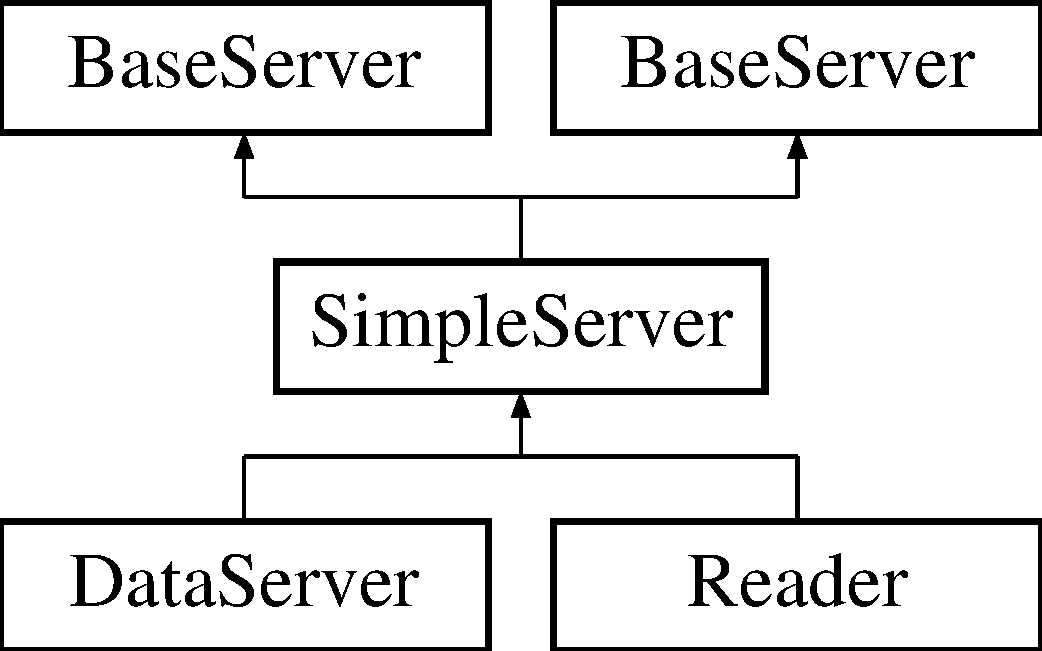
\includegraphics[height=3.000000cm]{classSimpleServer}
\end{center}
\end{figure}
\subsection*{Public Member Functions}
\begin{DoxyCompactItemize}
\item 
\hyperlink{classSimpleServer_aa4280135e2e20be8b8ae792e7119a061}{Simple\-Server} (unsigned short \hyperlink{classBaseServer_a66052c095234e31cada29b678b039c68}{port})
\item 
\hyperlink{classSimpleServer_aa4280135e2e20be8b8ae792e7119a061}{Simple\-Server} (unsigned short \hyperlink{classBaseServer_a66052c095234e31cada29b678b039c68}{port})
\end{DoxyCompactItemize}
\subsection*{Protected Member Functions}
\begin{DoxyCompactItemize}
\item 
virtual int \hyperlink{classSimpleServer_a1ff0dbc4a9c446fa4649410983b58311}{read\-\_\-from\-\_\-client} (int filedes)
\item 
virtual void \hyperlink{classSimpleServer_ad8244094d9e1806edaa166093c94bd24}{execute\-Cmd} (int client, short cmd, unsigned int $\ast$arg, short n)
\item 
virtual void \hyperlink{classSimpleServer_aabc58e7a255ae0efb25abdadbbaec527}{execute\-Cmd} (int client, short cmd, unsigned long $\ast$arg, short n)
\item 
virtual int \hyperlink{classSimpleServer_a1b032a7621374ef35a806af87253185a}{read\-\_\-from\-\_\-client} (int filedes)
\item 
virtual void \hyperlink{classSimpleServer_ad8244094d9e1806edaa166093c94bd24}{execute\-Cmd} (int client, short cmd, unsigned int $\ast$arg, short n)
\item 
virtual void \hyperlink{classSimpleServer_a4bbb57e575122b539fcddfa803cee206}{execute\-Cmd} (int client, short cmd, unsigned long $\ast$arg, short n)
\end{DoxyCompactItemize}
\subsection*{Additional Inherited Members}


\subsection{Detailed Description}
Implements a simple I\-P server.

The server waits for connections. The communication with the client is defined in the protected function read\-\_\-from\-\_\-client. Overload this function for a specific application.

The \hyperlink{classSimpleServer}{Simple\-Server} automatically detects the byte order of the client process and transfers all data in client byte order.

\begin{DoxyRefDesc}{Todo}
\item[\hyperlink{todo__todo000006}{Todo}]Use a independant threads for all connections. If one connection hangs, the other won't be affected?! 

Improve the Server managment. Loging, Shutdown via I\-P. For some other purpose a New class similar to Pbus/\-Pbus\-Proxy couble may be useful for mainanace and run control. Eg. Shutdown + restart of the Server, Control of the I\-Rdispatcher!!!\end{DoxyRefDesc}


Changes\-: \begin{DoxyItemize}
\item 30.\-8.\-05 ak\-: Detect client byte order \item 4.\-11.\-02 ak\-: Add stdin to the select functions. The server is now responding to socket and keyboard input! Improved output of the server -\/ format similar to that of netstat --ip. \item 31.\-10.\-02 ak\-: Closing all connected sockets before shutdown. This prevents hanging connections after terminating the server. \item 18.\-3.\-01 ak\-: Protected variable for the output stream introduced -\/ stop this nasty messages in the terminal!!!\end{DoxyItemize}
Implements a simple I\-P server.

The server waits for connections. The communication with the client is defined in the protected function read\-\_\-from\-\_\-client. Overload this function for a specific application.

The \hyperlink{classSimpleServer}{Simple\-Server} automatically detects the byte order of the client process and transfers all data in client byte order.

\begin{DoxyRefDesc}{Todo}
\item[\hyperlink{todo__todo000012}{Todo}]Use a independant threads for all connections. If one connection hangs, the other won't be affected?! 

Improve the Server managment. Loging, Shutdown via I\-P. For some other purpose a New class similar to Pbus/\-Pbus\-Proxy couble may be useful for mainanace and run control. Eg. Shutdown + restart of the Server, Control of the I\-Rdispatcher!!!\end{DoxyRefDesc}


Changes\-: \begin{DoxyItemize}
\item 30.\-8.\-05 ak\-: Detect client byte order \item 4.\-11.\-02 ak\-: Add stdin to the select functions. The server is now responding to socket and keyboard input! Improved output of the server -\/ format similar to that of netstat --ip. \item 31.\-10.\-02 ak\-: Closing all connected sockets before shutdown. This prevents hanging connections after terminating the server. \item 18.\-3.\-01 ak\-: Protected variable for the output stream introduced -\/ stop this nasty messages in the terminal!!! \end{DoxyItemize}


\subsection{Constructor \& Destructor Documentation}
\hypertarget{classSimpleServer_aa4280135e2e20be8b8ae792e7119a061}{\index{Simple\-Server@{Simple\-Server}!Simple\-Server@{Simple\-Server}}
\index{Simple\-Server@{Simple\-Server}!SimpleServer@{Simple\-Server}}
\subsubsection[{Simple\-Server}]{\setlength{\rightskip}{0pt plus 5cm}Simple\-Server\-::\-Simple\-Server (
\begin{DoxyParamCaption}
\item[{unsigned short}]{port}
\end{DoxyParamCaption}
)}}\label{classSimpleServer_aa4280135e2e20be8b8ae792e7119a061}
\hypertarget{classSimpleServer_aa4280135e2e20be8b8ae792e7119a061}{\index{Simple\-Server@{Simple\-Server}!Simple\-Server@{Simple\-Server}}
\index{Simple\-Server@{Simple\-Server}!SimpleServer@{Simple\-Server}}
\subsubsection[{Simple\-Server}]{\setlength{\rightskip}{0pt plus 5cm}Simple\-Server\-::\-Simple\-Server (
\begin{DoxyParamCaption}
\item[{unsigned short}]{port}
\end{DoxyParamCaption}
)}}\label{classSimpleServer_aa4280135e2e20be8b8ae792e7119a061}


\subsection{Member Function Documentation}
\hypertarget{classSimpleServer_ad8244094d9e1806edaa166093c94bd24}{\index{Simple\-Server@{Simple\-Server}!execute\-Cmd@{execute\-Cmd}}
\index{execute\-Cmd@{execute\-Cmd}!SimpleServer@{Simple\-Server}}
\subsubsection[{execute\-Cmd}]{\setlength{\rightskip}{0pt plus 5cm}virtual void Simple\-Server\-::execute\-Cmd (
\begin{DoxyParamCaption}
\item[{int}]{client, }
\item[{short}]{cmd, }
\item[{unsigned int $\ast$}]{arg, }
\item[{short}]{n}
\end{DoxyParamCaption}
)\hspace{0.3cm}{\ttfamily [protected]}, {\ttfamily [virtual]}}}\label{classSimpleServer_ad8244094d9e1806edaa166093c94bd24}
Execute a command -\/ The instruction set on the client side remote\-Call needs to fit to this implementation 

Reimplemented in \hyperlink{classDataServer_a726b0971e705894e243726640ecb7db0}{Data\-Server}, and \hyperlink{classReader_a8d71e1068d9bf3886ac4fd472ed71ae9}{Reader}.

\hypertarget{classSimpleServer_ad8244094d9e1806edaa166093c94bd24}{\index{Simple\-Server@{Simple\-Server}!execute\-Cmd@{execute\-Cmd}}
\index{execute\-Cmd@{execute\-Cmd}!SimpleServer@{Simple\-Server}}
\subsubsection[{execute\-Cmd}]{\setlength{\rightskip}{0pt plus 5cm}virtual void Simple\-Server\-::execute\-Cmd (
\begin{DoxyParamCaption}
\item[{int}]{client, }
\item[{short}]{cmd, }
\item[{unsigned int $\ast$}]{arg, }
\item[{short}]{n}
\end{DoxyParamCaption}
)\hspace{0.3cm}{\ttfamily [protected]}, {\ttfamily [virtual]}}}\label{classSimpleServer_ad8244094d9e1806edaa166093c94bd24}
Execute a command -\/ The instruction set on the client side remote\-Call needs to fit to this implementation 

Reimplemented in \hyperlink{classDataServer_a726b0971e705894e243726640ecb7db0}{Data\-Server}, and \hyperlink{classReader_a8d71e1068d9bf3886ac4fd472ed71ae9}{Reader}.

\hypertarget{classSimpleServer_a4bbb57e575122b539fcddfa803cee206}{\index{Simple\-Server@{Simple\-Server}!execute\-Cmd@{execute\-Cmd}}
\index{execute\-Cmd@{execute\-Cmd}!SimpleServer@{Simple\-Server}}
\subsubsection[{execute\-Cmd}]{\setlength{\rightskip}{0pt plus 5cm}virtual void Simple\-Server\-::execute\-Cmd (
\begin{DoxyParamCaption}
\item[{int}]{client, }
\item[{short}]{cmd, }
\item[{unsigned long $\ast$}]{arg, }
\item[{short}]{n}
\end{DoxyParamCaption}
)\hspace{0.3cm}{\ttfamily [protected]}, {\ttfamily [virtual]}}}\label{classSimpleServer_a4bbb57e575122b539fcddfa803cee206}
\hypertarget{classSimpleServer_aabc58e7a255ae0efb25abdadbbaec527}{\index{Simple\-Server@{Simple\-Server}!execute\-Cmd@{execute\-Cmd}}
\index{execute\-Cmd@{execute\-Cmd}!SimpleServer@{Simple\-Server}}
\subsubsection[{execute\-Cmd}]{\setlength{\rightskip}{0pt plus 5cm}void Simple\-Server\-::execute\-Cmd (
\begin{DoxyParamCaption}
\item[{int}]{client, }
\item[{short}]{cmd, }
\item[{unsigned long $\ast$}]{arg, }
\item[{short}]{n}
\end{DoxyParamCaption}
)\hspace{0.3cm}{\ttfamily [protected]}, {\ttfamily [virtual]}}}\label{classSimpleServer_aabc58e7a255ae0efb25abdadbbaec527}
\hypertarget{classSimpleServer_a1b032a7621374ef35a806af87253185a}{\index{Simple\-Server@{Simple\-Server}!read\-\_\-from\-\_\-client@{read\-\_\-from\-\_\-client}}
\index{read\-\_\-from\-\_\-client@{read\-\_\-from\-\_\-client}!SimpleServer@{Simple\-Server}}
\subsubsection[{read\-\_\-from\-\_\-client}]{\setlength{\rightskip}{0pt plus 5cm}virtual int Simple\-Server\-::read\-\_\-from\-\_\-client (
\begin{DoxyParamCaption}
\item[{int}]{filedes}
\end{DoxyParamCaption}
)\hspace{0.3cm}{\ttfamily [protected]}, {\ttfamily [virtual]}}}\label{classSimpleServer_a1b032a7621374ef35a806af87253185a}
Defines the interface from the communication with the proxy process. The function is able to detect if the client uses a different byte order and automatically re-\/orders the data. All following communication will be swapped to have the appropriate byte order.

The protocol is defined as follows\-: \begin{DoxyItemize}
\item command (4 bytes) \item len (4 bytes) \item data (len $\ast$ 4bytes) \end{DoxyItemize}


Reimplemented from \hyperlink{classBaseServer_a3e649e1a9564008b2728b429bcb7e192}{Base\-Server}.

\hypertarget{classSimpleServer_a1ff0dbc4a9c446fa4649410983b58311}{\index{Simple\-Server@{Simple\-Server}!read\-\_\-from\-\_\-client@{read\-\_\-from\-\_\-client}}
\index{read\-\_\-from\-\_\-client@{read\-\_\-from\-\_\-client}!SimpleServer@{Simple\-Server}}
\subsubsection[{read\-\_\-from\-\_\-client}]{\setlength{\rightskip}{0pt plus 5cm}int Simple\-Server\-::read\-\_\-from\-\_\-client (
\begin{DoxyParamCaption}
\item[{int}]{filedes}
\end{DoxyParamCaption}
)\hspace{0.3cm}{\ttfamily [protected]}, {\ttfamily [virtual]}}}\label{classSimpleServer_a1ff0dbc4a9c446fa4649410983b58311}
Defines the interface from the communication with the proxy process. The function is able to detect if the client uses a different byte order and automatically re-\/orders the data. All following communication will be swapped to have the appropriate byte order.

The protocol is defined as follows\-: \begin{DoxyItemize}
\item command (4 bytes) \item len (4 bytes) \item data (len $\ast$ 4bytes) \end{DoxyItemize}


Reimplemented from \hyperlink{classBaseServer_a3e649e1a9564008b2728b429bcb7e192}{Base\-Server}.



The documentation for this class was generated from the following files\-:\begin{DoxyCompactItemize}
\item 
/home/ntj/\-Development/phd/kitcube-\/tools/src/akutil/\hyperlink{simpleserver_8h}{simpleserver.\-h}\item 
/home/ntj/\-Development/phd/kitcube-\/tools/src/akutil.\-minimal/\hyperlink{minimal_2simpleserver_8h}{simpleserver.\-h}\item 
/home/ntj/\-Development/phd/kitcube-\/tools/src/akutil/\hyperlink{simpleserver_8cpp}{simpleserver.\-cpp}\item 
/home/ntj/\-Development/phd/kitcube-\/tools/src/akutil.\-minimal/\hyperlink{minimal_2simpleserver_8cpp}{simpleserver.\-cpp}\end{DoxyCompactItemize}

\hypertarget{classSimpleSocket}{\section{Simple\-Socket Class Reference}
\label{classSimpleSocket}\index{Simple\-Socket@{Simple\-Socket}}
}


{\ttfamily \#include $<$simplesocket.\-h$>$}

\subsection*{Public Member Functions}
\begin{DoxyCompactItemize}
\item 
\hyperlink{classSimpleSocket_ab743c534336f17d61023a808ec348877}{Simple\-Socket} (const char $\ast$server, unsigned short port)
\item 
\hyperlink{classSimpleSocket_aaaa3efe38c1c210643acd071115a8565}{Simple\-Socket} (const char $\ast$server, unsigned short port, unsigned long \hyperlink{classSimpleSocket_ac2e777bd36689f4f136b9c5b9e9c5f0e}{timeout})
\item 
\hyperlink{classSimpleSocket_a273bb8620aa05f75029f39e069e18e4f}{Simple\-Socket} (const char $\ast$server, unsigned short port, struct timeval \hyperlink{classSimpleSocket_ac2e777bd36689f4f136b9c5b9e9c5f0e}{timeout})
\item 
\hyperlink{classSimpleSocket_abf7d41536d2ecf56de1364d36db5fd67}{$\sim$\-Simple\-Socket} ()
\item 
void \hyperlink{classSimpleSocket_af8d68590cf2fd476dd7adf9681e68d1a}{set\-Timeout} (unsigned long \hyperlink{classSimpleSocket_ac2e777bd36689f4f136b9c5b9e9c5f0e}{timeout})
\item 
void \hyperlink{classSimpleSocket_aca833e1fd8c646100ba0c463ba68f527}{set\-Timeout} (struct timeval \hyperlink{classSimpleSocket_ac2e777bd36689f4f136b9c5b9e9c5f0e}{timeout})
\item 
int \hyperlink{classSimpleSocket_adf772ef82480b834bc3bc74ac0d21df9}{read\-Msg} (char $\ast$msg, int max)
\item 
int \hyperlink{classSimpleSocket_a095da277758577ab30ed76fabe130c89}{write\-Msg} (char $\ast$msg, int n=0)
\item 
int \hyperlink{classSimpleSocket_a8a8c2258b40fc70bc67405ef1f40e99b}{read\-Data} (unsigned long $\ast$data, int max)
\item 
int \hyperlink{classSimpleSocket_ab24262c3889678da11168ee6de116a28}{write\-Data} (unsigned long $\ast$data, int n)
\item 
int \hyperlink{classSimpleSocket_a9dd04548e098650a982ee8a4f44d080b}{read\-Data} (unsigned int $\ast$data, int max)
\item 
int \hyperlink{classSimpleSocket_aa8ece72de04ca74047b3a0b7f7a20484}{write\-Data} (unsigned int $\ast$data, int n)
\item 
char $\ast$ \hyperlink{classSimpleSocket_aa83abcf775e9638ffb9efe94472e841e}{get\-Host\-Name} ()
\item 
char $\ast$ \hyperlink{classSimpleSocket_ab04083cd52eb47f220a5a08d52b23ae5}{get\-Peer\-Name} ()
\item 
int \hyperlink{classSimpleSocket_af1de8044e016d3e6f0baf14a7130515f}{read\-Packet} (unsigned long $\ast$data, int max)
\item 
int \hyperlink{classSimpleSocket_a4c0227fb99f56767449617d88f1912bc}{write\-Packet} (unsigned long $\ast$data, int n)
\item 
int \hyperlink{classSimpleSocket_a861ec1830251182b7581c9db0a012c97}{remote\-Call} (short cmdid, unsigned long $\ast$args, short argc=0, unsigned long $\ast$data=N\-U\-L\-L, short ndata=0, unsigned long $\ast$ackn=N\-U\-L\-L, short len=0)
\item 
int \hyperlink{classSimpleSocket_aa707339f5e3cad2c475e9abbbea00328}{remote\-Call} (short cmdid, uint32\-\_\-t $\ast$args=N\-U\-L\-L, short argc=0, uint32\-\_\-t $\ast$data=N\-U\-L\-L, short ndata=0, uint32\-\_\-t $\ast$ackn=N\-U\-L\-L, short len=0)
\item 
int \hyperlink{classSimpleSocket_af9db6aa7c5c95cd00593cd73634a6adc}{wait\-For\-Reading} ()
\item 
int \hyperlink{classSimpleSocket_a27211c208598898ac3fcd9dd4b8dcd78}{wait\-For\-Writing} ()
\item 
int \hyperlink{classSimpleSocket_aa140f9d5c79130bd98da84a61cc2b285}{wait} (int \hyperlink{classSimpleSocket_ac2e777bd36689f4f136b9c5b9e9c5f0e}{timeout})
\item 
int \hyperlink{classSimpleSocket_abfe8170623b9a86f384433c37bae362d}{get\-F\-D} ()
\item 
\hyperlink{classSimpleSocket_ab743c534336f17d61023a808ec348877}{Simple\-Socket} (const char $\ast$server, unsigned short port)
\item 
\hyperlink{classSimpleSocket_aaaa3efe38c1c210643acd071115a8565}{Simple\-Socket} (const char $\ast$server, unsigned short port, unsigned long \hyperlink{classSimpleSocket_ac2e777bd36689f4f136b9c5b9e9c5f0e}{timeout})
\item 
\hyperlink{classSimpleSocket_a273bb8620aa05f75029f39e069e18e4f}{Simple\-Socket} (const char $\ast$server, unsigned short port, struct timeval \hyperlink{classSimpleSocket_ac2e777bd36689f4f136b9c5b9e9c5f0e}{timeout})
\item 
\hyperlink{classSimpleSocket_abf7d41536d2ecf56de1364d36db5fd67}{$\sim$\-Simple\-Socket} ()
\item 
void \hyperlink{classSimpleSocket_af8d68590cf2fd476dd7adf9681e68d1a}{set\-Timeout} (unsigned long \hyperlink{classSimpleSocket_ac2e777bd36689f4f136b9c5b9e9c5f0e}{timeout})
\item 
void \hyperlink{classSimpleSocket_aca833e1fd8c646100ba0c463ba68f527}{set\-Timeout} (struct timeval \hyperlink{classSimpleSocket_ac2e777bd36689f4f136b9c5b9e9c5f0e}{timeout})
\item 
int \hyperlink{classSimpleSocket_adf772ef82480b834bc3bc74ac0d21df9}{read\-Msg} (char $\ast$msg, int max)
\item 
int \hyperlink{classSimpleSocket_a095da277758577ab30ed76fabe130c89}{write\-Msg} (char $\ast$msg, int n=0)
\item 
int \hyperlink{classSimpleSocket_a8a8c2258b40fc70bc67405ef1f40e99b}{read\-Data} (unsigned long $\ast$data, int max)
\item 
int \hyperlink{classSimpleSocket_ab24262c3889678da11168ee6de116a28}{write\-Data} (unsigned long $\ast$data, int n)
\item 
int \hyperlink{classSimpleSocket_a9dd04548e098650a982ee8a4f44d080b}{read\-Data} (unsigned int $\ast$data, int max)
\item 
int \hyperlink{classSimpleSocket_aa8ece72de04ca74047b3a0b7f7a20484}{write\-Data} (unsigned int $\ast$data, int n)
\item 
char $\ast$ \hyperlink{classSimpleSocket_ab0e4f23eb7c541d6c8a062fecfdc2524}{get\-Host\-Name} ()
\item 
char $\ast$ \hyperlink{classSimpleSocket_aeb9df0d50ad09e65aaeba39b2372b1fd}{get\-Peer\-Name} ()
\item 
int \hyperlink{classSimpleSocket_af1de8044e016d3e6f0baf14a7130515f}{read\-Packet} (unsigned long $\ast$data, int max)
\item 
int \hyperlink{classSimpleSocket_a4c0227fb99f56767449617d88f1912bc}{write\-Packet} (unsigned long $\ast$data, int n)
\item 
int \hyperlink{classSimpleSocket_a861ec1830251182b7581c9db0a012c97}{remote\-Call} (short cmdid, unsigned long $\ast$args, short argc=0, unsigned long $\ast$data=N\-U\-L\-L, short ndata=0, unsigned long $\ast$ackn=N\-U\-L\-L, short len=0)
\item 
int \hyperlink{classSimpleSocket_aa707339f5e3cad2c475e9abbbea00328}{remote\-Call} (short cmdid, uint32\-\_\-t $\ast$args=N\-U\-L\-L, short argc=0, uint32\-\_\-t $\ast$data=N\-U\-L\-L, short ndata=0, uint32\-\_\-t $\ast$ackn=N\-U\-L\-L, short len=0)
\item 
int \hyperlink{classSimpleSocket_af9db6aa7c5c95cd00593cd73634a6adc}{wait\-For\-Reading} ()
\item 
int \hyperlink{classSimpleSocket_a27211c208598898ac3fcd9dd4b8dcd78}{wait\-For\-Writing} ()
\item 
int \hyperlink{classSimpleSocket_aa140f9d5c79130bd98da84a61cc2b285}{wait} (int \hyperlink{classSimpleSocket_ac2e777bd36689f4f136b9c5b9e9c5f0e}{timeout})
\item 
int \hyperlink{classSimpleSocket_abfe8170623b9a86f384433c37bae362d}{get\-F\-D} ()
\end{DoxyCompactItemize}
\subsection*{Private Member Functions}
\begin{DoxyCompactItemize}
\item 
void \hyperlink{classSimpleSocket_af082077fc1f725d9ba64f0ac429d02c8}{connect\-Server} (const char $\ast$server, unsigned short port)
\item 
void \hyperlink{classSimpleSocket_af082077fc1f725d9ba64f0ac429d02c8}{connect\-Server} (const char $\ast$server, unsigned short port)
\end{DoxyCompactItemize}
\subsection*{Private Attributes}
\begin{DoxyCompactItemize}
\item 
int \hyperlink{classSimpleSocket_a23557ce4b09fc521787340f38126b92e}{sock}
\item 
bool \hyperlink{classSimpleSocket_abbc193b9005628c260a53e864e6785cb}{nonblock}
\item 
struct timeval \hyperlink{classSimpleSocket_ac2e777bd36689f4f136b9c5b9e9c5f0e}{timeout}
\end{DoxyCompactItemize}


\subsection{Detailed Description}
Implements a simple socket for use with any server.

Every instance of the class will establish a connection with a server. By default the connection will use a timeout of S\-I\-M\-P\-L\-E\-S\-O\-C\-K\-E\-T\-\_\-\-T\-I\-M\-E\-O\-U\-T milliseconds. The timeout can be changed when using the socket connection with set\-Timeout. A value of zero for the timeout will turn off the timeout and makes every access blocking.

Changes\-: \begin{DoxyItemize}
\item Added timeout (8-\/2-\/2006 ak) \end{DoxyItemize}


\subsection{Constructor \& Destructor Documentation}
\hypertarget{classSimpleSocket_ab743c534336f17d61023a808ec348877}{\index{Simple\-Socket@{Simple\-Socket}!Simple\-Socket@{Simple\-Socket}}
\index{Simple\-Socket@{Simple\-Socket}!SimpleSocket@{Simple\-Socket}}
\subsubsection[{Simple\-Socket}]{\setlength{\rightskip}{0pt plus 5cm}Simple\-Socket\-::\-Simple\-Socket (
\begin{DoxyParamCaption}
\item[{const char $\ast$}]{server, }
\item[{unsigned short}]{port}
\end{DoxyParamCaption}
)}}\label{classSimpleSocket_ab743c534336f17d61023a808ec348877}
Create connection. There will be no timeout. To change the timeout after the connection is established use set\-Timeout function. 
\begin{DoxyParams}{Parameters}
{\em server} & hostname of the server application \\
\hline
{\em port} & port number of the server application \\
\hline
\end{DoxyParams}
\hypertarget{classSimpleSocket_aaaa3efe38c1c210643acd071115a8565}{\index{Simple\-Socket@{Simple\-Socket}!Simple\-Socket@{Simple\-Socket}}
\index{Simple\-Socket@{Simple\-Socket}!SimpleSocket@{Simple\-Socket}}
\subsubsection[{Simple\-Socket}]{\setlength{\rightskip}{0pt plus 5cm}Simple\-Socket\-::\-Simple\-Socket (
\begin{DoxyParamCaption}
\item[{const char $\ast$}]{server, }
\item[{unsigned short}]{port, }
\item[{unsigned long}]{timeout}
\end{DoxyParamCaption}
)}}\label{classSimpleSocket_aaaa3efe38c1c210643acd071115a8565}
Create connection with timeout To change the timeout after the connection is established use set\-Timeout function. 
\begin{DoxyParams}{Parameters}
{\em server} & hostname of the server application \\
\hline
{\em port} & port number of the server application \\
\hline
{\em timeout} & given in miliseconds \\
\hline
\end{DoxyParams}
\hypertarget{classSimpleSocket_a273bb8620aa05f75029f39e069e18e4f}{\index{Simple\-Socket@{Simple\-Socket}!Simple\-Socket@{Simple\-Socket}}
\index{Simple\-Socket@{Simple\-Socket}!SimpleSocket@{Simple\-Socket}}
\subsubsection[{Simple\-Socket}]{\setlength{\rightskip}{0pt plus 5cm}Simple\-Socket\-::\-Simple\-Socket (
\begin{DoxyParamCaption}
\item[{const char $\ast$}]{server, }
\item[{unsigned short}]{port, }
\item[{struct timeval}]{timeout}
\end{DoxyParamCaption}
)}}\label{classSimpleSocket_a273bb8620aa05f75029f39e069e18e4f}
Create connection with timeout To change the timeout after the connection is established use set\-Timeout function. 
\begin{DoxyParams}{Parameters}
{\em server} & hostname of the server application \\
\hline
{\em port} & port number of the server application \\
\hline
{\em timeout} & \\
\hline
\end{DoxyParams}
\hypertarget{classSimpleSocket_abf7d41536d2ecf56de1364d36db5fd67}{\index{Simple\-Socket@{Simple\-Socket}!$\sim$\-Simple\-Socket@{$\sim$\-Simple\-Socket}}
\index{$\sim$\-Simple\-Socket@{$\sim$\-Simple\-Socket}!SimpleSocket@{Simple\-Socket}}
\subsubsection[{$\sim$\-Simple\-Socket}]{\setlength{\rightskip}{0pt plus 5cm}Simple\-Socket\-::$\sim$\-Simple\-Socket (
\begin{DoxyParamCaption}
{}
\end{DoxyParamCaption}
)}}\label{classSimpleSocket_abf7d41536d2ecf56de1364d36db5fd67}
Destructor of class \hyperlink{classSimpleSocket}{Simple\-Socket}. \hypertarget{classSimpleSocket_ab743c534336f17d61023a808ec348877}{\index{Simple\-Socket@{Simple\-Socket}!Simple\-Socket@{Simple\-Socket}}
\index{Simple\-Socket@{Simple\-Socket}!SimpleSocket@{Simple\-Socket}}
\subsubsection[{Simple\-Socket}]{\setlength{\rightskip}{0pt plus 5cm}Simple\-Socket\-::\-Simple\-Socket (
\begin{DoxyParamCaption}
\item[{const char $\ast$}]{server, }
\item[{unsigned short}]{port}
\end{DoxyParamCaption}
)}}\label{classSimpleSocket_ab743c534336f17d61023a808ec348877}
Create connection. There will be no timeout. To change the timeout after the connection is established use set\-Timeout function. 
\begin{DoxyParams}{Parameters}
{\em server} & hostname of the server application \\
\hline
{\em port} & port number of the server application \\
\hline
\end{DoxyParams}
\hypertarget{classSimpleSocket_aaaa3efe38c1c210643acd071115a8565}{\index{Simple\-Socket@{Simple\-Socket}!Simple\-Socket@{Simple\-Socket}}
\index{Simple\-Socket@{Simple\-Socket}!SimpleSocket@{Simple\-Socket}}
\subsubsection[{Simple\-Socket}]{\setlength{\rightskip}{0pt plus 5cm}Simple\-Socket\-::\-Simple\-Socket (
\begin{DoxyParamCaption}
\item[{const char $\ast$}]{server, }
\item[{unsigned short}]{port, }
\item[{unsigned long}]{timeout}
\end{DoxyParamCaption}
)}}\label{classSimpleSocket_aaaa3efe38c1c210643acd071115a8565}
Create connection with timeout To change the timeout after the connection is established use set\-Timeout function. 
\begin{DoxyParams}{Parameters}
{\em server} & hostname of the server application \\
\hline
{\em port} & port number of the server application \\
\hline
{\em timeout} & given in miliseconds \\
\hline
\end{DoxyParams}
\hypertarget{classSimpleSocket_a273bb8620aa05f75029f39e069e18e4f}{\index{Simple\-Socket@{Simple\-Socket}!Simple\-Socket@{Simple\-Socket}}
\index{Simple\-Socket@{Simple\-Socket}!SimpleSocket@{Simple\-Socket}}
\subsubsection[{Simple\-Socket}]{\setlength{\rightskip}{0pt plus 5cm}Simple\-Socket\-::\-Simple\-Socket (
\begin{DoxyParamCaption}
\item[{const char $\ast$}]{server, }
\item[{unsigned short}]{port, }
\item[{struct timeval}]{timeout}
\end{DoxyParamCaption}
)}}\label{classSimpleSocket_a273bb8620aa05f75029f39e069e18e4f}
Create connection with timeout To change the timeout after the connection is established use set\-Timeout function. 
\begin{DoxyParams}{Parameters}
{\em server} & hostname of the server application \\
\hline
{\em port} & port number of the server application \\
\hline
{\em timeout} & \\
\hline
\end{DoxyParams}
\hypertarget{classSimpleSocket_abf7d41536d2ecf56de1364d36db5fd67}{\index{Simple\-Socket@{Simple\-Socket}!$\sim$\-Simple\-Socket@{$\sim$\-Simple\-Socket}}
\index{$\sim$\-Simple\-Socket@{$\sim$\-Simple\-Socket}!SimpleSocket@{Simple\-Socket}}
\subsubsection[{$\sim$\-Simple\-Socket}]{\setlength{\rightskip}{0pt plus 5cm}Simple\-Socket\-::$\sim$\-Simple\-Socket (
\begin{DoxyParamCaption}
{}
\end{DoxyParamCaption}
)}}\label{classSimpleSocket_abf7d41536d2ecf56de1364d36db5fd67}
Destructor of class \hyperlink{classSimpleSocket}{Simple\-Socket}. 

\subsection{Member Function Documentation}
\hypertarget{classSimpleSocket_af082077fc1f725d9ba64f0ac429d02c8}{\index{Simple\-Socket@{Simple\-Socket}!connect\-Server@{connect\-Server}}
\index{connect\-Server@{connect\-Server}!SimpleSocket@{Simple\-Socket}}
\subsubsection[{connect\-Server}]{\setlength{\rightskip}{0pt plus 5cm}void Simple\-Socket\-::connect\-Server (
\begin{DoxyParamCaption}
\item[{const char $\ast$}]{server, }
\item[{unsigned short}]{port}
\end{DoxyParamCaption}
)\hspace{0.3cm}{\ttfamily [private]}}}\label{classSimpleSocket_af082077fc1f725d9ba64f0ac429d02c8}
Connect to server \hypertarget{classSimpleSocket_af082077fc1f725d9ba64f0ac429d02c8}{\index{Simple\-Socket@{Simple\-Socket}!connect\-Server@{connect\-Server}}
\index{connect\-Server@{connect\-Server}!SimpleSocket@{Simple\-Socket}}
\subsubsection[{connect\-Server}]{\setlength{\rightskip}{0pt plus 5cm}void Simple\-Socket\-::connect\-Server (
\begin{DoxyParamCaption}
\item[{const char $\ast$}]{server, }
\item[{unsigned short}]{port}
\end{DoxyParamCaption}
)\hspace{0.3cm}{\ttfamily [private]}}}\label{classSimpleSocket_af082077fc1f725d9ba64f0ac429d02c8}
Connect to server \hypertarget{classSimpleSocket_abfe8170623b9a86f384433c37bae362d}{\index{Simple\-Socket@{Simple\-Socket}!get\-F\-D@{get\-F\-D}}
\index{get\-F\-D@{get\-F\-D}!SimpleSocket@{Simple\-Socket}}
\subsubsection[{get\-F\-D}]{\setlength{\rightskip}{0pt plus 5cm}int Simple\-Socket\-::get\-F\-D (
\begin{DoxyParamCaption}
{}
\end{DoxyParamCaption}
)}}\label{classSimpleSocket_abfe8170623b9a86f384433c37bae362d}
Get the file desciptor \hypertarget{classSimpleSocket_abfe8170623b9a86f384433c37bae362d}{\index{Simple\-Socket@{Simple\-Socket}!get\-F\-D@{get\-F\-D}}
\index{get\-F\-D@{get\-F\-D}!SimpleSocket@{Simple\-Socket}}
\subsubsection[{get\-F\-D}]{\setlength{\rightskip}{0pt plus 5cm}int Simple\-Socket\-::get\-F\-D (
\begin{DoxyParamCaption}
{}
\end{DoxyParamCaption}
)}}\label{classSimpleSocket_abfe8170623b9a86f384433c37bae362d}
Get the file desciptor \hypertarget{classSimpleSocket_aa83abcf775e9638ffb9efe94472e841e}{\index{Simple\-Socket@{Simple\-Socket}!get\-Host\-Name@{get\-Host\-Name}}
\index{get\-Host\-Name@{get\-Host\-Name}!SimpleSocket@{Simple\-Socket}}
\subsubsection[{get\-Host\-Name}]{\setlength{\rightskip}{0pt plus 5cm}char $\ast$ Simple\-Socket\-::get\-Host\-Name (
\begin{DoxyParamCaption}
{}
\end{DoxyParamCaption}
)}}\label{classSimpleSocket_aa83abcf775e9638ffb9efe94472e841e}
\hypertarget{classSimpleSocket_ab0e4f23eb7c541d6c8a062fecfdc2524}{\index{Simple\-Socket@{Simple\-Socket}!get\-Host\-Name@{get\-Host\-Name}}
\index{get\-Host\-Name@{get\-Host\-Name}!SimpleSocket@{Simple\-Socket}}
\subsubsection[{get\-Host\-Name}]{\setlength{\rightskip}{0pt plus 5cm}char$\ast$ Simple\-Socket\-::get\-Host\-Name (
\begin{DoxyParamCaption}
{}
\end{DoxyParamCaption}
)}}\label{classSimpleSocket_ab0e4f23eb7c541d6c8a062fecfdc2524}
\hypertarget{classSimpleSocket_ab04083cd52eb47f220a5a08d52b23ae5}{\index{Simple\-Socket@{Simple\-Socket}!get\-Peer\-Name@{get\-Peer\-Name}}
\index{get\-Peer\-Name@{get\-Peer\-Name}!SimpleSocket@{Simple\-Socket}}
\subsubsection[{get\-Peer\-Name}]{\setlength{\rightskip}{0pt plus 5cm}char $\ast$ Simple\-Socket\-::get\-Peer\-Name (
\begin{DoxyParamCaption}
{}
\end{DoxyParamCaption}
)}}\label{classSimpleSocket_ab04083cd52eb47f220a5a08d52b23ae5}
\hypertarget{classSimpleSocket_aeb9df0d50ad09e65aaeba39b2372b1fd}{\index{Simple\-Socket@{Simple\-Socket}!get\-Peer\-Name@{get\-Peer\-Name}}
\index{get\-Peer\-Name@{get\-Peer\-Name}!SimpleSocket@{Simple\-Socket}}
\subsubsection[{get\-Peer\-Name}]{\setlength{\rightskip}{0pt plus 5cm}char$\ast$ Simple\-Socket\-::get\-Peer\-Name (
\begin{DoxyParamCaption}
{}
\end{DoxyParamCaption}
)}}\label{classSimpleSocket_aeb9df0d50ad09e65aaeba39b2372b1fd}
\hypertarget{classSimpleSocket_a8a8c2258b40fc70bc67405ef1f40e99b}{\index{Simple\-Socket@{Simple\-Socket}!read\-Data@{read\-Data}}
\index{read\-Data@{read\-Data}!SimpleSocket@{Simple\-Socket}}
\subsubsection[{read\-Data}]{\setlength{\rightskip}{0pt plus 5cm}int Simple\-Socket\-::read\-Data (
\begin{DoxyParamCaption}
\item[{unsigned long $\ast$}]{data, }
\item[{int}]{max}
\end{DoxyParamCaption}
)}}\label{classSimpleSocket_a8a8c2258b40fc70bc67405ef1f40e99b}
\hypertarget{classSimpleSocket_a8a8c2258b40fc70bc67405ef1f40e99b}{\index{Simple\-Socket@{Simple\-Socket}!read\-Data@{read\-Data}}
\index{read\-Data@{read\-Data}!SimpleSocket@{Simple\-Socket}}
\subsubsection[{read\-Data}]{\setlength{\rightskip}{0pt plus 5cm}int Simple\-Socket\-::read\-Data (
\begin{DoxyParamCaption}
\item[{unsigned long $\ast$}]{data, }
\item[{int}]{max}
\end{DoxyParamCaption}
)}}\label{classSimpleSocket_a8a8c2258b40fc70bc67405ef1f40e99b}
\hypertarget{classSimpleSocket_a9dd04548e098650a982ee8a4f44d080b}{\index{Simple\-Socket@{Simple\-Socket}!read\-Data@{read\-Data}}
\index{read\-Data@{read\-Data}!SimpleSocket@{Simple\-Socket}}
\subsubsection[{read\-Data}]{\setlength{\rightskip}{0pt plus 5cm}int Simple\-Socket\-::read\-Data (
\begin{DoxyParamCaption}
\item[{unsigned int $\ast$}]{data, }
\item[{int}]{max}
\end{DoxyParamCaption}
)}}\label{classSimpleSocket_a9dd04548e098650a982ee8a4f44d080b}
\hypertarget{classSimpleSocket_a9dd04548e098650a982ee8a4f44d080b}{\index{Simple\-Socket@{Simple\-Socket}!read\-Data@{read\-Data}}
\index{read\-Data@{read\-Data}!SimpleSocket@{Simple\-Socket}}
\subsubsection[{read\-Data}]{\setlength{\rightskip}{0pt plus 5cm}int Simple\-Socket\-::read\-Data (
\begin{DoxyParamCaption}
\item[{unsigned int $\ast$}]{data, }
\item[{int}]{max}
\end{DoxyParamCaption}
)}}\label{classSimpleSocket_a9dd04548e098650a982ee8a4f44d080b}
\hypertarget{classSimpleSocket_adf772ef82480b834bc3bc74ac0d21df9}{\index{Simple\-Socket@{Simple\-Socket}!read\-Msg@{read\-Msg}}
\index{read\-Msg@{read\-Msg}!SimpleSocket@{Simple\-Socket}}
\subsubsection[{read\-Msg}]{\setlength{\rightskip}{0pt plus 5cm}int Simple\-Socket\-::read\-Msg (
\begin{DoxyParamCaption}
\item[{char $\ast$}]{msg, }
\item[{int}]{max}
\end{DoxyParamCaption}
)}}\label{classSimpleSocket_adf772ef82480b834bc3bc74ac0d21df9}
\hypertarget{classSimpleSocket_adf772ef82480b834bc3bc74ac0d21df9}{\index{Simple\-Socket@{Simple\-Socket}!read\-Msg@{read\-Msg}}
\index{read\-Msg@{read\-Msg}!SimpleSocket@{Simple\-Socket}}
\subsubsection[{read\-Msg}]{\setlength{\rightskip}{0pt plus 5cm}int Simple\-Socket\-::read\-Msg (
\begin{DoxyParamCaption}
\item[{char $\ast$}]{msg, }
\item[{int}]{max}
\end{DoxyParamCaption}
)}}\label{classSimpleSocket_adf772ef82480b834bc3bc74ac0d21df9}
\hypertarget{classSimpleSocket_af1de8044e016d3e6f0baf14a7130515f}{\index{Simple\-Socket@{Simple\-Socket}!read\-Packet@{read\-Packet}}
\index{read\-Packet@{read\-Packet}!SimpleSocket@{Simple\-Socket}}
\subsubsection[{read\-Packet}]{\setlength{\rightskip}{0pt plus 5cm}int Simple\-Socket\-::read\-Packet (
\begin{DoxyParamCaption}
\item[{unsigned long $\ast$}]{data, }
\item[{int}]{max}
\end{DoxyParamCaption}
)}}\label{classSimpleSocket_af1de8044e016d3e6f0baf14a7130515f}
Read a packet of raw data. Each packet consist of header, raw data and trailer. Header and trailer have the format 0xfff $|$ length of raw data. \hypertarget{classSimpleSocket_af1de8044e016d3e6f0baf14a7130515f}{\index{Simple\-Socket@{Simple\-Socket}!read\-Packet@{read\-Packet}}
\index{read\-Packet@{read\-Packet}!SimpleSocket@{Simple\-Socket}}
\subsubsection[{read\-Packet}]{\setlength{\rightskip}{0pt plus 5cm}int Simple\-Socket\-::read\-Packet (
\begin{DoxyParamCaption}
\item[{unsigned long $\ast$}]{data, }
\item[{int}]{max}
\end{DoxyParamCaption}
)}}\label{classSimpleSocket_af1de8044e016d3e6f0baf14a7130515f}
Read a packet of raw data. Each packet consist of header, raw data and trailer. Header and trailer have the format 0xfff $|$ length of raw data. \hypertarget{classSimpleSocket_a861ec1830251182b7581c9db0a012c97}{\index{Simple\-Socket@{Simple\-Socket}!remote\-Call@{remote\-Call}}
\index{remote\-Call@{remote\-Call}!SimpleSocket@{Simple\-Socket}}
\subsubsection[{remote\-Call}]{\setlength{\rightskip}{0pt plus 5cm}int Simple\-Socket\-::remote\-Call (
\begin{DoxyParamCaption}
\item[{short}]{cmdid, }
\item[{unsigned long $\ast$}]{args, }
\item[{short}]{argc = {\ttfamily 0}, }
\item[{unsigned long $\ast$}]{data = {\ttfamily NULL}, }
\item[{short}]{ndata = {\ttfamily 0}, }
\item[{unsigned long $\ast$}]{ackn = {\ttfamily NULL}, }
\item[{short}]{len = {\ttfamily 0}}
\end{DoxyParamCaption}
)}}\label{classSimpleSocket_a861ec1830251182b7581c9db0a012c97}
Make a call to the connected server. The command implements a simple protokoll to exchange command id, arguments and results. The command also considers possible error messages.


\begin{DoxyParams}{Parameters}
{\em cmdid} & Command id; has to be implemented by higher level protokolls \\
\hline
{\em args} & List of arguments \\
\hline
{\em argc} & Number of arguments in lists args \\
\hline
{\em data} & List of data \\
\hline
{\em ndata} & Number of data \\
\hline
{\em ackn} & List of acknowledge parameter \\
\hline
{\em len} & Number acknowledge parameter\\
\hline
\end{DoxyParams}
\begin{DoxyReturn}{Returns}
error status\-: 0 no error, 1+ error while exectution of the command, -\/1 socket communication closed by foreign host. 
\end{DoxyReturn}
\hypertarget{classSimpleSocket_a861ec1830251182b7581c9db0a012c97}{\index{Simple\-Socket@{Simple\-Socket}!remote\-Call@{remote\-Call}}
\index{remote\-Call@{remote\-Call}!SimpleSocket@{Simple\-Socket}}
\subsubsection[{remote\-Call}]{\setlength{\rightskip}{0pt plus 5cm}int Simple\-Socket\-::remote\-Call (
\begin{DoxyParamCaption}
\item[{short}]{cmdid, }
\item[{unsigned long $\ast$}]{args, }
\item[{short}]{argc = {\ttfamily 0}, }
\item[{unsigned long $\ast$}]{data = {\ttfamily NULL}, }
\item[{short}]{ndata = {\ttfamily 0}, }
\item[{unsigned long $\ast$}]{ackn = {\ttfamily NULL}, }
\item[{short}]{len = {\ttfamily 0}}
\end{DoxyParamCaption}
)}}\label{classSimpleSocket_a861ec1830251182b7581c9db0a012c97}
Make a call to the connected server. The command implements a simple protokoll to exchange command id, arguments and results. The command also considers possible error messages.


\begin{DoxyParams}{Parameters}
{\em cmdid} & Command id; has to be implemented by higher level protokolls \\
\hline
{\em args} & List of arguments \\
\hline
{\em argc} & Number of arguments in lists args \\
\hline
{\em data} & List of data \\
\hline
{\em ndata} & Number of data \\
\hline
{\em ackn} & List of acknowledge parameter \\
\hline
{\em len} & Number acknowledge parameter\\
\hline
\end{DoxyParams}
\begin{DoxyReturn}{Returns}
error status\-: 0 no error, 1+ error while exectution of the command, -\/1 socket communication closed by foreign host. 
\end{DoxyReturn}
\hypertarget{classSimpleSocket_aa707339f5e3cad2c475e9abbbea00328}{\index{Simple\-Socket@{Simple\-Socket}!remote\-Call@{remote\-Call}}
\index{remote\-Call@{remote\-Call}!SimpleSocket@{Simple\-Socket}}
\subsubsection[{remote\-Call}]{\setlength{\rightskip}{0pt plus 5cm}int Simple\-Socket\-::remote\-Call (
\begin{DoxyParamCaption}
\item[{short}]{cmdid, }
\item[{uint32\-\_\-t $\ast$}]{args = {\ttfamily NULL}, }
\item[{short}]{argc = {\ttfamily 0}, }
\item[{uint32\-\_\-t $\ast$}]{data = {\ttfamily NULL}, }
\item[{short}]{ndata = {\ttfamily 0}, }
\item[{uint32\-\_\-t $\ast$}]{ackn = {\ttfamily NULL}, }
\item[{short}]{len = {\ttfamily 0}}
\end{DoxyParamCaption}
)}}\label{classSimpleSocket_aa707339f5e3cad2c475e9abbbea00328}
\hypertarget{classSimpleSocket_aa707339f5e3cad2c475e9abbbea00328}{\index{Simple\-Socket@{Simple\-Socket}!remote\-Call@{remote\-Call}}
\index{remote\-Call@{remote\-Call}!SimpleSocket@{Simple\-Socket}}
\subsubsection[{remote\-Call}]{\setlength{\rightskip}{0pt plus 5cm}int Simple\-Socket\-::remote\-Call (
\begin{DoxyParamCaption}
\item[{short}]{cmdid, }
\item[{uint32\-\_\-t $\ast$}]{args = {\ttfamily NULL}, }
\item[{short}]{argc = {\ttfamily 0}, }
\item[{uint32\-\_\-t $\ast$}]{data = {\ttfamily NULL}, }
\item[{short}]{ndata = {\ttfamily 0}, }
\item[{uint32\-\_\-t $\ast$}]{ackn = {\ttfamily NULL}, }
\item[{short}]{len = {\ttfamily 0}}
\end{DoxyParamCaption}
)}}\label{classSimpleSocket_aa707339f5e3cad2c475e9abbbea00328}
\hypertarget{classSimpleSocket_af8d68590cf2fd476dd7adf9681e68d1a}{\index{Simple\-Socket@{Simple\-Socket}!set\-Timeout@{set\-Timeout}}
\index{set\-Timeout@{set\-Timeout}!SimpleSocket@{Simple\-Socket}}
\subsubsection[{set\-Timeout}]{\setlength{\rightskip}{0pt plus 5cm}void Simple\-Socket\-::set\-Timeout (
\begin{DoxyParamCaption}
\item[{unsigned long}]{timeout}
\end{DoxyParamCaption}
)}}\label{classSimpleSocket_af8d68590cf2fd476dd7adf9681e68d1a}
Set timeout in miliseconds \hypertarget{classSimpleSocket_af8d68590cf2fd476dd7adf9681e68d1a}{\index{Simple\-Socket@{Simple\-Socket}!set\-Timeout@{set\-Timeout}}
\index{set\-Timeout@{set\-Timeout}!SimpleSocket@{Simple\-Socket}}
\subsubsection[{set\-Timeout}]{\setlength{\rightskip}{0pt plus 5cm}void Simple\-Socket\-::set\-Timeout (
\begin{DoxyParamCaption}
\item[{unsigned long}]{timeout}
\end{DoxyParamCaption}
)}}\label{classSimpleSocket_af8d68590cf2fd476dd7adf9681e68d1a}
Set timeout in miliseconds \hypertarget{classSimpleSocket_aca833e1fd8c646100ba0c463ba68f527}{\index{Simple\-Socket@{Simple\-Socket}!set\-Timeout@{set\-Timeout}}
\index{set\-Timeout@{set\-Timeout}!SimpleSocket@{Simple\-Socket}}
\subsubsection[{set\-Timeout}]{\setlength{\rightskip}{0pt plus 5cm}void Simple\-Socket\-::set\-Timeout (
\begin{DoxyParamCaption}
\item[{struct timeval}]{timeout}
\end{DoxyParamCaption}
)}}\label{classSimpleSocket_aca833e1fd8c646100ba0c463ba68f527}
Set timeout \hypertarget{classSimpleSocket_aca833e1fd8c646100ba0c463ba68f527}{\index{Simple\-Socket@{Simple\-Socket}!set\-Timeout@{set\-Timeout}}
\index{set\-Timeout@{set\-Timeout}!SimpleSocket@{Simple\-Socket}}
\subsubsection[{set\-Timeout}]{\setlength{\rightskip}{0pt plus 5cm}void Simple\-Socket\-::set\-Timeout (
\begin{DoxyParamCaption}
\item[{struct timeval}]{timeout}
\end{DoxyParamCaption}
)}}\label{classSimpleSocket_aca833e1fd8c646100ba0c463ba68f527}
Set timeout \hypertarget{classSimpleSocket_aa140f9d5c79130bd98da84a61cc2b285}{\index{Simple\-Socket@{Simple\-Socket}!wait@{wait}}
\index{wait@{wait}!SimpleSocket@{Simple\-Socket}}
\subsubsection[{wait}]{\setlength{\rightskip}{0pt plus 5cm}int Simple\-Socket\-::wait (
\begin{DoxyParamCaption}
\item[{int}]{timeout}
\end{DoxyParamCaption}
)}}\label{classSimpleSocket_aa140f9d5c79130bd98da84a61cc2b285}
Wait for a certain time


\begin{DoxyParams}{Parameters}
{\em timeout} & Time to wait in seconds \\
\hline
\end{DoxyParams}
\hypertarget{classSimpleSocket_aa140f9d5c79130bd98da84a61cc2b285}{\index{Simple\-Socket@{Simple\-Socket}!wait@{wait}}
\index{wait@{wait}!SimpleSocket@{Simple\-Socket}}
\subsubsection[{wait}]{\setlength{\rightskip}{0pt plus 5cm}int Simple\-Socket\-::wait (
\begin{DoxyParamCaption}
\item[{int}]{timeout}
\end{DoxyParamCaption}
)}}\label{classSimpleSocket_aa140f9d5c79130bd98da84a61cc2b285}
Wait for a certain time


\begin{DoxyParams}{Parameters}
{\em timeout} & Time to wait in seconds \\
\hline
\end{DoxyParams}
\hypertarget{classSimpleSocket_af9db6aa7c5c95cd00593cd73634a6adc}{\index{Simple\-Socket@{Simple\-Socket}!wait\-For\-Reading@{wait\-For\-Reading}}
\index{wait\-For\-Reading@{wait\-For\-Reading}!SimpleSocket@{Simple\-Socket}}
\subsubsection[{wait\-For\-Reading}]{\setlength{\rightskip}{0pt plus 5cm}int Simple\-Socket\-::wait\-For\-Reading (
\begin{DoxyParamCaption}
{}
\end{DoxyParamCaption}
)}}\label{classSimpleSocket_af9db6aa7c5c95cd00593cd73634a6adc}
Wait for reading socket.

\begin{DoxyReturn}{Returns}
-\/1 error, 0 timeout, 1 ok 
\end{DoxyReturn}
\hypertarget{classSimpleSocket_af9db6aa7c5c95cd00593cd73634a6adc}{\index{Simple\-Socket@{Simple\-Socket}!wait\-For\-Reading@{wait\-For\-Reading}}
\index{wait\-For\-Reading@{wait\-For\-Reading}!SimpleSocket@{Simple\-Socket}}
\subsubsection[{wait\-For\-Reading}]{\setlength{\rightskip}{0pt plus 5cm}int Simple\-Socket\-::wait\-For\-Reading (
\begin{DoxyParamCaption}
{}
\end{DoxyParamCaption}
)}}\label{classSimpleSocket_af9db6aa7c5c95cd00593cd73634a6adc}
Wait for reading socket.

\begin{DoxyReturn}{Returns}
-\/1 error, 0 timeout, 1 ok 
\end{DoxyReturn}
\hypertarget{classSimpleSocket_a27211c208598898ac3fcd9dd4b8dcd78}{\index{Simple\-Socket@{Simple\-Socket}!wait\-For\-Writing@{wait\-For\-Writing}}
\index{wait\-For\-Writing@{wait\-For\-Writing}!SimpleSocket@{Simple\-Socket}}
\subsubsection[{wait\-For\-Writing}]{\setlength{\rightskip}{0pt plus 5cm}int Simple\-Socket\-::wait\-For\-Writing (
\begin{DoxyParamCaption}
{}
\end{DoxyParamCaption}
)}}\label{classSimpleSocket_a27211c208598898ac3fcd9dd4b8dcd78}
Wait for reading socket.

\begin{DoxyReturn}{Returns}
-\/1 error, 0 timeout, 1 ok 
\end{DoxyReturn}
\hypertarget{classSimpleSocket_a27211c208598898ac3fcd9dd4b8dcd78}{\index{Simple\-Socket@{Simple\-Socket}!wait\-For\-Writing@{wait\-For\-Writing}}
\index{wait\-For\-Writing@{wait\-For\-Writing}!SimpleSocket@{Simple\-Socket}}
\subsubsection[{wait\-For\-Writing}]{\setlength{\rightskip}{0pt plus 5cm}int Simple\-Socket\-::wait\-For\-Writing (
\begin{DoxyParamCaption}
{}
\end{DoxyParamCaption}
)}}\label{classSimpleSocket_a27211c208598898ac3fcd9dd4b8dcd78}
Wait for reading socket.

\begin{DoxyReturn}{Returns}
-\/1 error, 0 timeout, 1 ok 
\end{DoxyReturn}
\hypertarget{classSimpleSocket_ab24262c3889678da11168ee6de116a28}{\index{Simple\-Socket@{Simple\-Socket}!write\-Data@{write\-Data}}
\index{write\-Data@{write\-Data}!SimpleSocket@{Simple\-Socket}}
\subsubsection[{write\-Data}]{\setlength{\rightskip}{0pt plus 5cm}int Simple\-Socket\-::write\-Data (
\begin{DoxyParamCaption}
\item[{unsigned long $\ast$}]{data, }
\item[{int}]{n}
\end{DoxyParamCaption}
)}}\label{classSimpleSocket_ab24262c3889678da11168ee6de116a28}
\hypertarget{classSimpleSocket_ab24262c3889678da11168ee6de116a28}{\index{Simple\-Socket@{Simple\-Socket}!write\-Data@{write\-Data}}
\index{write\-Data@{write\-Data}!SimpleSocket@{Simple\-Socket}}
\subsubsection[{write\-Data}]{\setlength{\rightskip}{0pt plus 5cm}int Simple\-Socket\-::write\-Data (
\begin{DoxyParamCaption}
\item[{unsigned long $\ast$}]{data, }
\item[{int}]{n}
\end{DoxyParamCaption}
)}}\label{classSimpleSocket_ab24262c3889678da11168ee6de116a28}
\hypertarget{classSimpleSocket_aa8ece72de04ca74047b3a0b7f7a20484}{\index{Simple\-Socket@{Simple\-Socket}!write\-Data@{write\-Data}}
\index{write\-Data@{write\-Data}!SimpleSocket@{Simple\-Socket}}
\subsubsection[{write\-Data}]{\setlength{\rightskip}{0pt plus 5cm}int Simple\-Socket\-::write\-Data (
\begin{DoxyParamCaption}
\item[{unsigned int $\ast$}]{data, }
\item[{int}]{n}
\end{DoxyParamCaption}
)}}\label{classSimpleSocket_aa8ece72de04ca74047b3a0b7f7a20484}
\hypertarget{classSimpleSocket_aa8ece72de04ca74047b3a0b7f7a20484}{\index{Simple\-Socket@{Simple\-Socket}!write\-Data@{write\-Data}}
\index{write\-Data@{write\-Data}!SimpleSocket@{Simple\-Socket}}
\subsubsection[{write\-Data}]{\setlength{\rightskip}{0pt plus 5cm}int Simple\-Socket\-::write\-Data (
\begin{DoxyParamCaption}
\item[{unsigned int $\ast$}]{data, }
\item[{int}]{n}
\end{DoxyParamCaption}
)}}\label{classSimpleSocket_aa8ece72de04ca74047b3a0b7f7a20484}
\hypertarget{classSimpleSocket_a095da277758577ab30ed76fabe130c89}{\index{Simple\-Socket@{Simple\-Socket}!write\-Msg@{write\-Msg}}
\index{write\-Msg@{write\-Msg}!SimpleSocket@{Simple\-Socket}}
\subsubsection[{write\-Msg}]{\setlength{\rightskip}{0pt plus 5cm}int Simple\-Socket\-::write\-Msg (
\begin{DoxyParamCaption}
\item[{char $\ast$}]{msg, }
\item[{int}]{n = {\ttfamily 0}}
\end{DoxyParamCaption}
)}}\label{classSimpleSocket_a095da277758577ab30ed76fabe130c89}
\hypertarget{classSimpleSocket_a095da277758577ab30ed76fabe130c89}{\index{Simple\-Socket@{Simple\-Socket}!write\-Msg@{write\-Msg}}
\index{write\-Msg@{write\-Msg}!SimpleSocket@{Simple\-Socket}}
\subsubsection[{write\-Msg}]{\setlength{\rightskip}{0pt plus 5cm}int Simple\-Socket\-::write\-Msg (
\begin{DoxyParamCaption}
\item[{char $\ast$}]{msg, }
\item[{int}]{n = {\ttfamily 0}}
\end{DoxyParamCaption}
)}}\label{classSimpleSocket_a095da277758577ab30ed76fabe130c89}
\hypertarget{classSimpleSocket_a4c0227fb99f56767449617d88f1912bc}{\index{Simple\-Socket@{Simple\-Socket}!write\-Packet@{write\-Packet}}
\index{write\-Packet@{write\-Packet}!SimpleSocket@{Simple\-Socket}}
\subsubsection[{write\-Packet}]{\setlength{\rightskip}{0pt plus 5cm}int Simple\-Socket\-::write\-Packet (
\begin{DoxyParamCaption}
\item[{unsigned long $\ast$}]{data, }
\item[{int}]{n}
\end{DoxyParamCaption}
)}}\label{classSimpleSocket_a4c0227fb99f56767449617d88f1912bc}
Write a packet of raw data. Each packet consist of header, raw data and trailer. Header and trailer have the format 0xfff $|$ length of raw data. \hypertarget{classSimpleSocket_a4c0227fb99f56767449617d88f1912bc}{\index{Simple\-Socket@{Simple\-Socket}!write\-Packet@{write\-Packet}}
\index{write\-Packet@{write\-Packet}!SimpleSocket@{Simple\-Socket}}
\subsubsection[{write\-Packet}]{\setlength{\rightskip}{0pt plus 5cm}int Simple\-Socket\-::write\-Packet (
\begin{DoxyParamCaption}
\item[{unsigned long $\ast$}]{data, }
\item[{int}]{n}
\end{DoxyParamCaption}
)}}\label{classSimpleSocket_a4c0227fb99f56767449617d88f1912bc}
Write a packet of raw data. Each packet consist of header, raw data and trailer. Header and trailer have the format 0xfff $|$ length of raw data. 

\subsection{Member Data Documentation}
\hypertarget{classSimpleSocket_abbc193b9005628c260a53e864e6785cb}{\index{Simple\-Socket@{Simple\-Socket}!nonblock@{nonblock}}
\index{nonblock@{nonblock}!SimpleSocket@{Simple\-Socket}}
\subsubsection[{nonblock}]{\setlength{\rightskip}{0pt plus 5cm}bool Simple\-Socket\-::nonblock\hspace{0.3cm}{\ttfamily [private]}}}\label{classSimpleSocket_abbc193b9005628c260a53e864e6785cb}
Flag to indicate nonblocking sockets. \hypertarget{classSimpleSocket_a23557ce4b09fc521787340f38126b92e}{\index{Simple\-Socket@{Simple\-Socket}!sock@{sock}}
\index{sock@{sock}!SimpleSocket@{Simple\-Socket}}
\subsubsection[{sock}]{\setlength{\rightskip}{0pt plus 5cm}int Simple\-Socket\-::sock\hspace{0.3cm}{\ttfamily [private]}}}\label{classSimpleSocket_a23557ce4b09fc521787340f38126b92e}
\hypertarget{classSimpleSocket_ac2e777bd36689f4f136b9c5b9e9c5f0e}{\index{Simple\-Socket@{Simple\-Socket}!timeout@{timeout}}
\index{timeout@{timeout}!SimpleSocket@{Simple\-Socket}}
\subsubsection[{timeout}]{\setlength{\rightskip}{0pt plus 5cm}struct timeval Simple\-Socket\-::timeout\hspace{0.3cm}{\ttfamily [private]}}}\label{classSimpleSocket_ac2e777bd36689f4f136b9c5b9e9c5f0e}
Timeout for connection, reading and writing. 

The documentation for this class was generated from the following files\-:\begin{DoxyCompactItemize}
\item 
/home/ntj/\-Development/phd/kitcube-\/tools/src/akutil/\hyperlink{simplesocket_8h}{simplesocket.\-h}\item 
/home/ntj/\-Development/phd/kitcube-\/tools/src/akutil.\-minimal/\hyperlink{minimal_2simplesocket_8h}{simplesocket.\-h}\item 
/home/ntj/\-Development/phd/kitcube-\/tools/src/akutil/\hyperlink{simplesocket_8cpp}{simplesocket.\-cpp}\item 
/home/ntj/\-Development/phd/kitcube-\/tools/src/akutil.\-minimal/\hyperlink{minimal_2simplesocket_8cpp}{simplesocket.\-cpp}\end{DoxyCompactItemize}

\hypertarget{classSimRandom}{\section{Sim\-Random Class Reference}
\label{classSimRandom}\index{Sim\-Random@{Sim\-Random}}
}


{\ttfamily \#include $<$simrandom.\-h$>$}

Inheritance diagram for Sim\-Random\-:\begin{figure}[H]
\begin{center}
\leavevmode
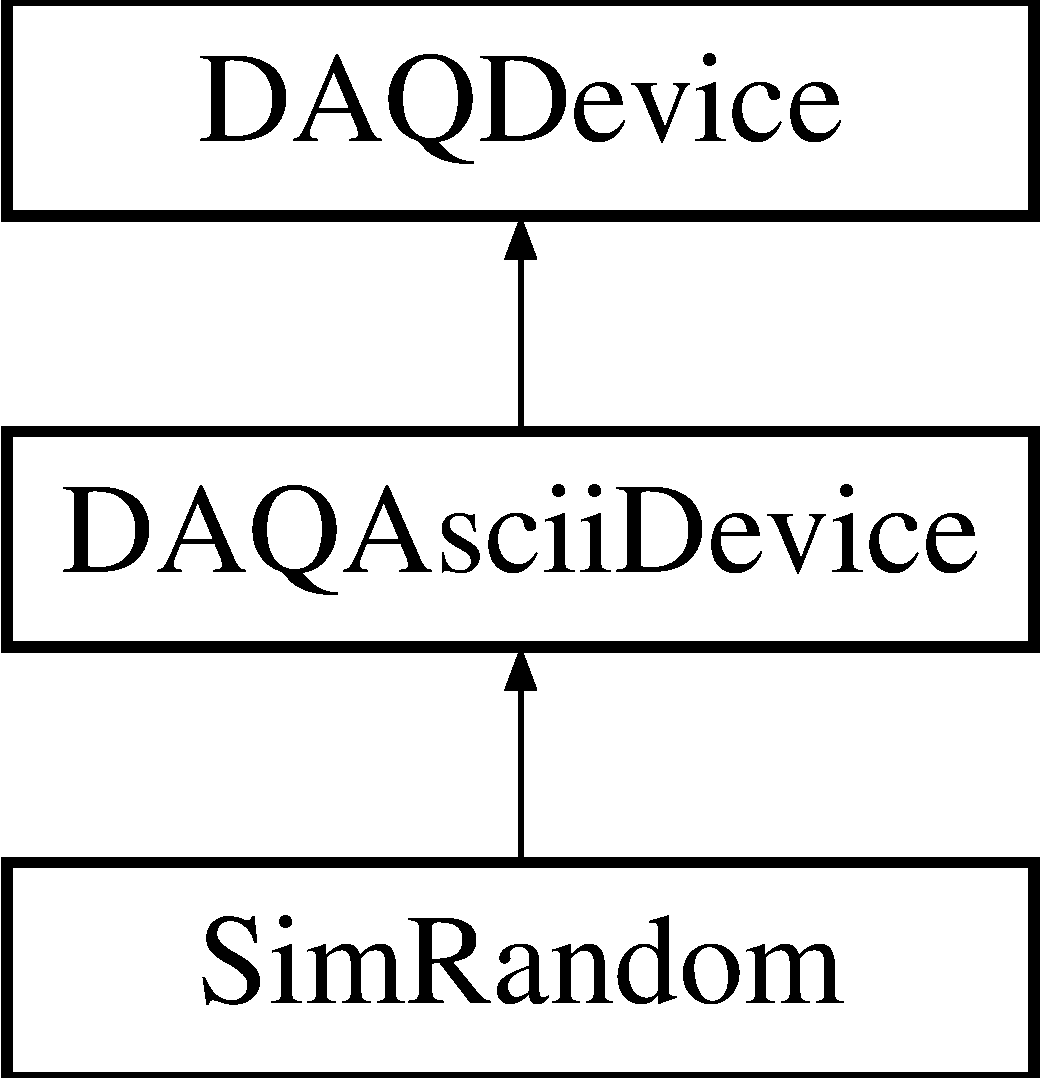
\includegraphics[height=3.000000cm]{classSimRandom}
\end{center}
\end{figure}
\subsection*{Public Member Functions}
\begin{DoxyCompactItemize}
\item 
\hyperlink{classSimRandom_a734a95f856d89911c75d83e464fa2579}{Sim\-Random} ()
\item 
\hyperlink{classSimRandom_ae5a11688acf03196c76b5b6774bc2a75}{$\sim$\-Sim\-Random} ()
\item 
void \hyperlink{classSimRandom_a48019bace7da9b182ef482e135b6736e}{set\-Config\-Defaults} ()
\item 
const char $\ast$ \hyperlink{classSimRandom_a5d4693d599a13efe8a75cf72dd55d8f3}{get\-Data\-Dir} ()
\item 
int \hyperlink{classSimRandom_a2a652b85ec23f610491f5f838664f152}{read\-Header} (const char $\ast$\hyperlink{classDAQDevice_a7f9cda7cf5b41f6b134c313477e9644b}{filename})
\item 
void \hyperlink{classSimRandom_a5119c39c479a46a691fe63b3b388c3fc}{write\-Header} ()
\item 
int \hyperlink{classSimRandom_a239bacabadccabc3c6d32278ab357ac1}{parse\-Data} (char $\ast$line, struct timeval $\ast$l\-\_\-t\-Data, double $\ast$\hyperlink{classDAQDevice_ad148188c57598fdf4fd4c1c333aeb0d8}{sensor\-Value})
\item 
void \hyperlink{classSimRandom_a8ef2df7e35047cee952340901a96aba4}{write\-Data} ()
\item 
const char $\ast$ \hyperlink{classSimRandom_ae456d364f9f6eda82fa7947cb3ccd813}{get\-Data\-Filename} ()
\end{DoxyCompactItemize}
\subsection*{Additional Inherited Members}


\subsection{Detailed Description}
Implementation for the weather mast D\-A\-Q devices that are used for turbulence, energy balance and 20m mast. 

\subsection{Constructor \& Destructor Documentation}
\hypertarget{classSimRandom_a734a95f856d89911c75d83e464fa2579}{\index{Sim\-Random@{Sim\-Random}!Sim\-Random@{Sim\-Random}}
\index{Sim\-Random@{Sim\-Random}!SimRandom@{Sim\-Random}}
\subsubsection[{Sim\-Random}]{\setlength{\rightskip}{0pt plus 5cm}Sim\-Random\-::\-Sim\-Random (
\begin{DoxyParamCaption}
{}
\end{DoxyParamCaption}
)}}\label{classSimRandom_a734a95f856d89911c75d83e464fa2579}
\hypertarget{classSimRandom_ae5a11688acf03196c76b5b6774bc2a75}{\index{Sim\-Random@{Sim\-Random}!$\sim$\-Sim\-Random@{$\sim$\-Sim\-Random}}
\index{$\sim$\-Sim\-Random@{$\sim$\-Sim\-Random}!SimRandom@{Sim\-Random}}
\subsubsection[{$\sim$\-Sim\-Random}]{\setlength{\rightskip}{0pt plus 5cm}Sim\-Random\-::$\sim$\-Sim\-Random (
\begin{DoxyParamCaption}
{}
\end{DoxyParamCaption}
)}}\label{classSimRandom_ae5a11688acf03196c76b5b6774bc2a75}


\subsection{Member Function Documentation}
\hypertarget{classSimRandom_a5d4693d599a13efe8a75cf72dd55d8f3}{\index{Sim\-Random@{Sim\-Random}!get\-Data\-Dir@{get\-Data\-Dir}}
\index{get\-Data\-Dir@{get\-Data\-Dir}!SimRandom@{Sim\-Random}}
\subsubsection[{get\-Data\-Dir}]{\setlength{\rightskip}{0pt plus 5cm}const char $\ast$ Sim\-Random\-::get\-Data\-Dir (
\begin{DoxyParamCaption}
{}
\end{DoxyParamCaption}
)\hspace{0.3cm}{\ttfamily [virtual]}}}\label{classSimRandom_a5d4693d599a13efe8a75cf72dd55d8f3}


Reimplemented from \hyperlink{classDAQDevice_a7d7d41f0c1496221e589d84b38d1c865}{D\-A\-Q\-Device}.

\hypertarget{classSimRandom_ae456d364f9f6eda82fa7947cb3ccd813}{\index{Sim\-Random@{Sim\-Random}!get\-Data\-Filename@{get\-Data\-Filename}}
\index{get\-Data\-Filename@{get\-Data\-Filename}!SimRandom@{Sim\-Random}}
\subsubsection[{get\-Data\-Filename}]{\setlength{\rightskip}{0pt plus 5cm}const char $\ast$ Sim\-Random\-::get\-Data\-Filename (
\begin{DoxyParamCaption}
{}
\end{DoxyParamCaption}
)\hspace{0.3cm}{\ttfamily [virtual]}}}\label{classSimRandom_ae456d364f9f6eda82fa7947cb3ccd813}
Implements the data filename convention of the D\-A\-Q module. 

Reimplemented from \hyperlink{classDAQDevice_af4734900eb86417b3160a723a077f8f5}{D\-A\-Q\-Device}.

\hypertarget{classSimRandom_a239bacabadccabc3c6d32278ab357ac1}{\index{Sim\-Random@{Sim\-Random}!parse\-Data@{parse\-Data}}
\index{parse\-Data@{parse\-Data}!SimRandom@{Sim\-Random}}
\subsubsection[{parse\-Data}]{\setlength{\rightskip}{0pt plus 5cm}int Sim\-Random\-::parse\-Data (
\begin{DoxyParamCaption}
\item[{char $\ast$}]{line, }
\item[{struct timeval $\ast$}]{l\-\_\-t\-Data, }
\item[{double $\ast$}]{sensor\-Value}
\end{DoxyParamCaption}
)\hspace{0.3cm}{\ttfamily [virtual]}}}\label{classSimRandom_a239bacabadccabc3c6d32278ab357ac1}
Read the data from the current line of the data file. \begin{DoxyReturn}{Returns}
-\/1 no data found, skip storage 0 sucess, store data, 1 read another line 
\end{DoxyReturn}


Reimplemented from \hyperlink{classDAQAsciiDevice_a9c20d9d69af4ba1641dbc82dd5be2aa5}{D\-A\-Q\-Ascii\-Device}.

\hypertarget{classSimRandom_a2a652b85ec23f610491f5f838664f152}{\index{Sim\-Random@{Sim\-Random}!read\-Header@{read\-Header}}
\index{read\-Header@{read\-Header}!SimRandom@{Sim\-Random}}
\subsubsection[{read\-Header}]{\setlength{\rightskip}{0pt plus 5cm}int Sim\-Random\-::read\-Header (
\begin{DoxyParamCaption}
\item[{const char $\ast$}]{filename}
\end{DoxyParamCaption}
)\hspace{0.3cm}{\ttfamily [virtual]}}}\label{classSimRandom_a2a652b85ec23f610491f5f838664f152}
Get time until next sample and it's id 

Reimplemented from \hyperlink{classDAQAsciiDevice_a5fce725c52b70ef2f56a34b32a03e15d}{D\-A\-Q\-Ascii\-Device}.

\hypertarget{classSimRandom_a48019bace7da9b182ef482e135b6736e}{\index{Sim\-Random@{Sim\-Random}!set\-Config\-Defaults@{set\-Config\-Defaults}}
\index{set\-Config\-Defaults@{set\-Config\-Defaults}!SimRandom@{Sim\-Random}}
\subsubsection[{set\-Config\-Defaults}]{\setlength{\rightskip}{0pt plus 5cm}void Sim\-Random\-::set\-Config\-Defaults (
\begin{DoxyParamCaption}
{}
\end{DoxyParamCaption}
)\hspace{0.3cm}{\ttfamily [virtual]}}}\label{classSimRandom_a48019bace7da9b182ef482e135b6736e}
The function is called before reading the configuration from the inifile. Use this fucntion in the module specific implementation to override the standard defaults 

Reimplemented from \hyperlink{classDAQDevice_a7685cec80865752cc0ef3ab49c6c2277}{D\-A\-Q\-Device}.

\hypertarget{classSimRandom_a8ef2df7e35047cee952340901a96aba4}{\index{Sim\-Random@{Sim\-Random}!write\-Data@{write\-Data}}
\index{write\-Data@{write\-Data}!SimRandom@{Sim\-Random}}
\subsubsection[{write\-Data}]{\setlength{\rightskip}{0pt plus 5cm}void Sim\-Random\-::write\-Data (
\begin{DoxyParamCaption}
{}
\end{DoxyParamCaption}
)\hspace{0.3cm}{\ttfamily [virtual]}}}\label{classSimRandom_a8ef2df7e35047cee952340901a96aba4}


Reimplemented from \hyperlink{classDAQDevice_acdc9d3765b1dfd845f99ec9c93071811}{D\-A\-Q\-Device}.

\hypertarget{classSimRandom_a5119c39c479a46a691fe63b3b388c3fc}{\index{Sim\-Random@{Sim\-Random}!write\-Header@{write\-Header}}
\index{write\-Header@{write\-Header}!SimRandom@{Sim\-Random}}
\subsubsection[{write\-Header}]{\setlength{\rightskip}{0pt plus 5cm}void Sim\-Random\-::write\-Header (
\begin{DoxyParamCaption}
{}
\end{DoxyParamCaption}
)\hspace{0.3cm}{\ttfamily [virtual]}}}\label{classSimRandom_a5119c39c479a46a691fe63b3b388c3fc}


Reimplemented from \hyperlink{classDAQDevice_aad39c13f039abd6e6a9b0aa21a7c8a4d}{D\-A\-Q\-Device}.



The documentation for this class was generated from the following files\-:\begin{DoxyCompactItemize}
\item 
/home/ntj/\-Development/phd/kitcube-\/tools/src/kitcube-\/devices/\hyperlink{simrandom_8h}{simrandom.\-h}\item 
/home/ntj/\-Development/phd/kitcube-\/tools/src/kitcube-\/devices/\hyperlink{simrandom_8cpp}{simrandom.\-cpp}\end{DoxyCompactItemize}

\hypertarget{classsisomop}{\section{sisomop Class Reference}
\label{classsisomop}\index{sisomop@{sisomop}}
}


{\ttfamily \#include $<$sisomop.\-h$>$}

Inheritance diagram for sisomop\-:\begin{figure}[H]
\begin{center}
\leavevmode
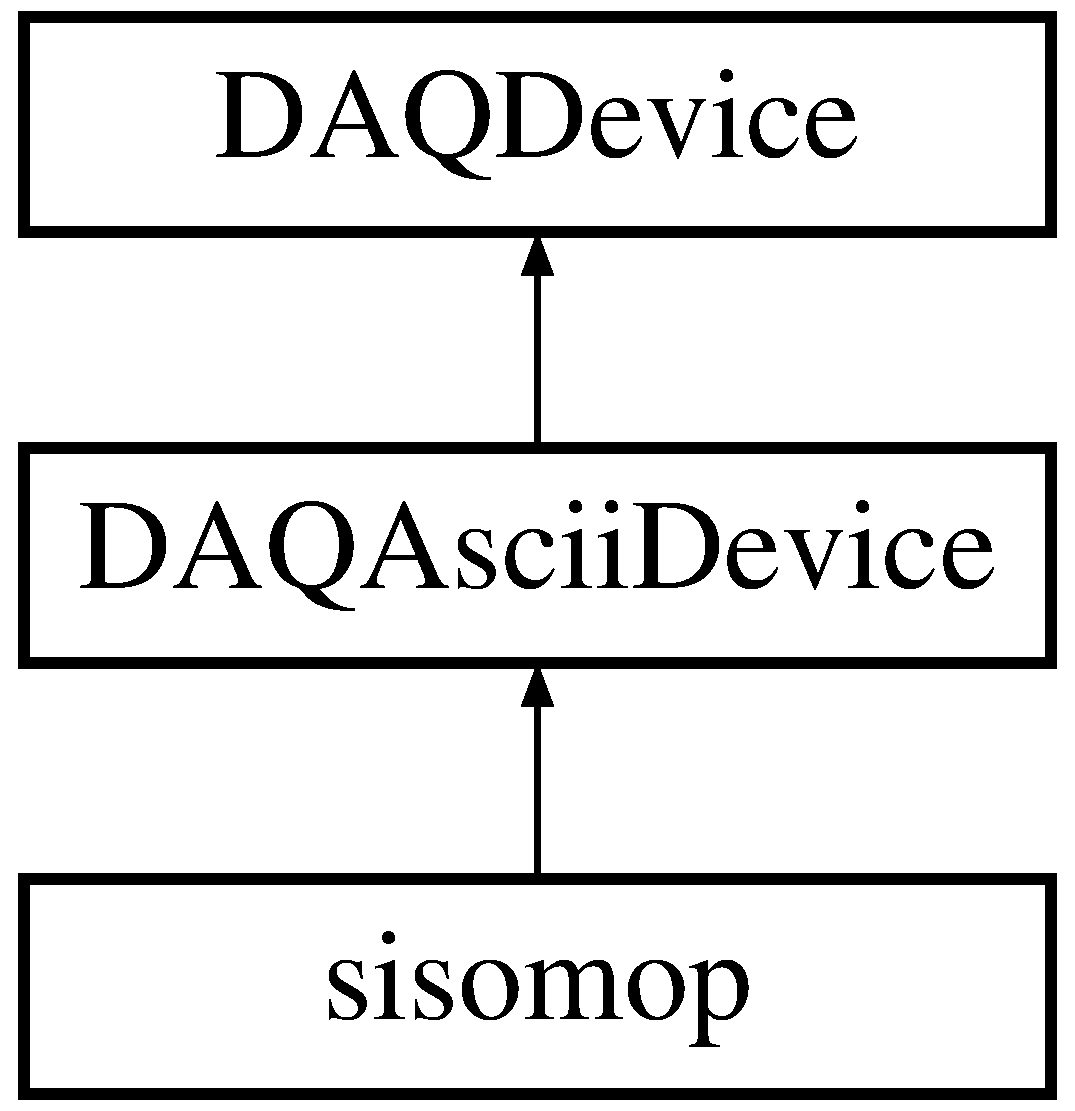
\includegraphics[height=3.000000cm]{classsisomop}
\end{center}
\end{figure}
\subsection*{Public Member Functions}
\begin{DoxyCompactItemize}
\item 
\hyperlink{classsisomop_a243e702fdb0d3610bc7c019840551d1f}{sisomop} ()
\item 
\hyperlink{classsisomop_a9fa5295780f44baa15987437b8b0e742}{$\sim$sisomop} ()
\item 
void \hyperlink{classsisomop_a388047e129e1c7082a8d9e99e2e8ec99}{set\-Config\-Defaults} ()
\item 
const char $\ast$ \hyperlink{classsisomop_a3f242e161d194348f13d8a4b399e23a3}{get\-Data\-Dir} ()
\item 
int \hyperlink{classsisomop_a658a1ebe29f6405d2aabb7b3ce335fdd}{read\-Header} (const char $\ast$\hyperlink{classDAQDevice_a7f9cda7cf5b41f6b134c313477e9644b}{filename})
\item 
int \hyperlink{classsisomop_a8c2afe6fe5aac3e8b8e860f3589407c1}{parse\-Data} (char $\ast$line, struct timeval $\ast$l\-\_\-t\-Data, double $\ast$\hyperlink{classDAQDevice_ad148188c57598fdf4fd4c1c333aeb0d8}{sensor\-Value})
\item 
unsigned int \hyperlink{classsisomop_ac80a0cb371d6419d2dcd6bdc3b93cc6d}{get\-Sensor\-Group} ()
\end{DoxyCompactItemize}
\subsection*{Additional Inherited Members}


\subsection{Detailed Description}
Implementation for the soil moisture sensors (Simple Soil Moisture Probe (S\-I\-S\-O\-M\-O\-P) ) 

\subsection{Constructor \& Destructor Documentation}
\hypertarget{classsisomop_a243e702fdb0d3610bc7c019840551d1f}{\index{sisomop@{sisomop}!sisomop@{sisomop}}
\index{sisomop@{sisomop}!sisomop@{sisomop}}
\subsubsection[{sisomop}]{\setlength{\rightskip}{0pt plus 5cm}sisomop\-::sisomop (
\begin{DoxyParamCaption}
{}
\end{DoxyParamCaption}
)}}\label{classsisomop_a243e702fdb0d3610bc7c019840551d1f}
\hypertarget{classsisomop_a9fa5295780f44baa15987437b8b0e742}{\index{sisomop@{sisomop}!$\sim$sisomop@{$\sim$sisomop}}
\index{$\sim$sisomop@{$\sim$sisomop}!sisomop@{sisomop}}
\subsubsection[{$\sim$sisomop}]{\setlength{\rightskip}{0pt plus 5cm}sisomop\-::$\sim$sisomop (
\begin{DoxyParamCaption}
{}
\end{DoxyParamCaption}
)}}\label{classsisomop_a9fa5295780f44baa15987437b8b0e742}


\subsection{Member Function Documentation}
\hypertarget{classsisomop_a3f242e161d194348f13d8a4b399e23a3}{\index{sisomop@{sisomop}!get\-Data\-Dir@{get\-Data\-Dir}}
\index{get\-Data\-Dir@{get\-Data\-Dir}!sisomop@{sisomop}}
\subsubsection[{get\-Data\-Dir}]{\setlength{\rightskip}{0pt plus 5cm}const char $\ast$ sisomop\-::get\-Data\-Dir (
\begin{DoxyParamCaption}
{}
\end{DoxyParamCaption}
)\hspace{0.3cm}{\ttfamily [virtual]}}}\label{classsisomop_a3f242e161d194348f13d8a4b399e23a3}
Returns the path relative to the base path to the data dir 

Reimplemented from \hyperlink{classDAQDevice_a7d7d41f0c1496221e589d84b38d1c865}{D\-A\-Q\-Device}.

\hypertarget{classsisomop_ac80a0cb371d6419d2dcd6bdc3b93cc6d}{\index{sisomop@{sisomop}!get\-Sensor\-Group@{get\-Sensor\-Group}}
\index{get\-Sensor\-Group@{get\-Sensor\-Group}!sisomop@{sisomop}}
\subsubsection[{get\-Sensor\-Group}]{\setlength{\rightskip}{0pt plus 5cm}unsigned int sisomop\-::get\-Sensor\-Group (
\begin{DoxyParamCaption}
{}
\end{DoxyParamCaption}
)\hspace{0.3cm}{\ttfamily [virtual]}}}\label{classsisomop_ac80a0cb371d6419d2dcd6bdc3b93cc6d}
Define a sensor group number for all the availble sensor group files 

Reimplemented from \hyperlink{classDAQDevice_a61d08492a11c30944dfaf3b86115abe8}{D\-A\-Q\-Device}.

\hypertarget{classsisomop_a8c2afe6fe5aac3e8b8e860f3589407c1}{\index{sisomop@{sisomop}!parse\-Data@{parse\-Data}}
\index{parse\-Data@{parse\-Data}!sisomop@{sisomop}}
\subsubsection[{parse\-Data}]{\setlength{\rightskip}{0pt plus 5cm}int sisomop\-::parse\-Data (
\begin{DoxyParamCaption}
\item[{char $\ast$}]{line, }
\item[{struct timeval $\ast$}]{l\-\_\-t\-Data, }
\item[{double $\ast$}]{sensor\-Value}
\end{DoxyParamCaption}
)\hspace{0.3cm}{\ttfamily [virtual]}}}\label{classsisomop_a8c2afe6fe5aac3e8b8e860f3589407c1}
Read the data from the current line of the data file. \begin{DoxyReturn}{Returns}
-\/1 no data found, skip storage 0 sucess, store data, 1 read another line 
\end{DoxyReturn}


Reimplemented from \hyperlink{classDAQAsciiDevice_a9c20d9d69af4ba1641dbc82dd5be2aa5}{D\-A\-Q\-Ascii\-Device}.

\hypertarget{classsisomop_a658a1ebe29f6405d2aabb7b3ce335fdd}{\index{sisomop@{sisomop}!read\-Header@{read\-Header}}
\index{read\-Header@{read\-Header}!sisomop@{sisomop}}
\subsubsection[{read\-Header}]{\setlength{\rightskip}{0pt plus 5cm}int sisomop\-::read\-Header (
\begin{DoxyParamCaption}
\item[{const char $\ast$}]{header}
\end{DoxyParamCaption}
)\hspace{0.3cm}{\ttfamily [virtual]}}}\label{classsisomop_a658a1ebe29f6405d2aabb7b3ce335fdd}
Get time until next sample and it's id 

Reimplemented from \hyperlink{classDAQAsciiDevice_a5fce725c52b70ef2f56a34b32a03e15d}{D\-A\-Q\-Ascii\-Device}.

\hypertarget{classsisomop_a388047e129e1c7082a8d9e99e2e8ec99}{\index{sisomop@{sisomop}!set\-Config\-Defaults@{set\-Config\-Defaults}}
\index{set\-Config\-Defaults@{set\-Config\-Defaults}!sisomop@{sisomop}}
\subsubsection[{set\-Config\-Defaults}]{\setlength{\rightskip}{0pt plus 5cm}void sisomop\-::set\-Config\-Defaults (
\begin{DoxyParamCaption}
{}
\end{DoxyParamCaption}
)\hspace{0.3cm}{\ttfamily [virtual]}}}\label{classsisomop_a388047e129e1c7082a8d9e99e2e8ec99}
The function is called before reading the configuration from the inifile. Use this fucntion in the module specific implementation to override the standard defaults 

Reimplemented from \hyperlink{classDAQDevice_a7685cec80865752cc0ef3ab49c6c2277}{D\-A\-Q\-Device}.



The documentation for this class was generated from the following files\-:\begin{DoxyCompactItemize}
\item 
/home/ntj/\-Development/phd/kitcube-\/tools/src/kitcube-\/devices/\hyperlink{sisomop_8h}{sisomop.\-h}\item 
/home/ntj/\-Development/phd/kitcube-\/tools/src/kitcube-\/devices/\hyperlink{sisomop_8cpp}{sisomop.\-cpp}\end{DoxyCompactItemize}

\hypertarget{classSocketServer}{\section{Socket\-Server Class Reference}
\label{classSocketServer}\index{Socket\-Server@{Socket\-Server}}
}


{\ttfamily \#include $<$socketserver.\-h$>$}

\subsection*{Public Member Functions}
\begin{DoxyCompactItemize}
\item 
\hyperlink{classSocketServer_a262ba93dc8ad71b260fb75124b3453ee}{Socket\-Server} ()
\item 
\hyperlink{classSocketServer_af0e595690e453ef4b8e8da174069aba9}{$\sim$\-Socket\-Server} ()
\end{DoxyCompactItemize}


\subsection{Detailed Description}
\begin{DoxyAuthor}{Author}
A Kopmann 
\end{DoxyAuthor}


\subsection{Constructor \& Destructor Documentation}
\hypertarget{classSocketServer_a262ba93dc8ad71b260fb75124b3453ee}{\index{Socket\-Server@{Socket\-Server}!Socket\-Server@{Socket\-Server}}
\index{Socket\-Server@{Socket\-Server}!SocketServer@{Socket\-Server}}
\subsubsection[{Socket\-Server}]{\setlength{\rightskip}{0pt plus 5cm}Socket\-Server\-::\-Socket\-Server (
\begin{DoxyParamCaption}
{}
\end{DoxyParamCaption}
)}}\label{classSocketServer_a262ba93dc8ad71b260fb75124b3453ee}
\hypertarget{classSocketServer_af0e595690e453ef4b8e8da174069aba9}{\index{Socket\-Server@{Socket\-Server}!$\sim$\-Socket\-Server@{$\sim$\-Socket\-Server}}
\index{$\sim$\-Socket\-Server@{$\sim$\-Socket\-Server}!SocketServer@{Socket\-Server}}
\subsubsection[{$\sim$\-Socket\-Server}]{\setlength{\rightskip}{0pt plus 5cm}Socket\-Server\-::$\sim$\-Socket\-Server (
\begin{DoxyParamCaption}
{}
\end{DoxyParamCaption}
)}}\label{classSocketServer_af0e595690e453ef4b8e8da174069aba9}


The documentation for this class was generated from the following files\-:\begin{DoxyCompactItemize}
\item 
/home/ntj/\-Development/phd/kitcube-\/tools/src/akutil/\hyperlink{socketserver_8h}{socketserver.\-h}\item 
/home/ntj/\-Development/phd/kitcube-\/tools/src/akutil/\hyperlink{socketserver_8cpp}{socketserver.\-cpp}\end{DoxyCompactItemize}

\hypertarget{classsodar}{\section{sodar Class Reference}
\label{classsodar}\index{sodar@{sodar}}
}


{\ttfamily \#include $<$sodar.\-h$>$}

Inheritance diagram for sodar\-:\begin{figure}[H]
\begin{center}
\leavevmode
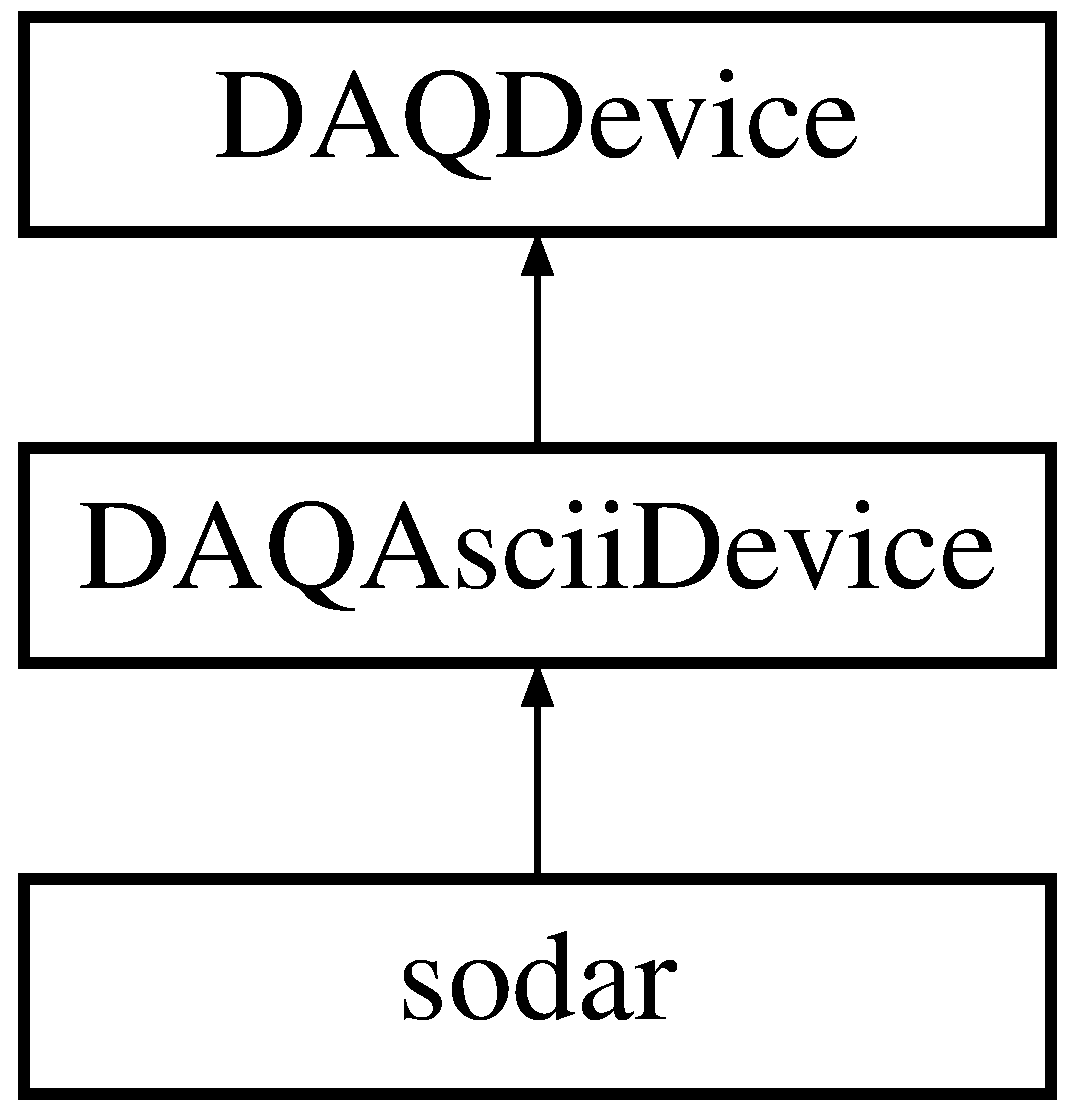
\includegraphics[height=3.000000cm]{classsodar}
\end{center}
\end{figure}
\subsection*{Public Member Functions}
\begin{DoxyCompactItemize}
\item 
\hyperlink{classsodar_a8aaddca894ce6fe0f8ce57c1f4a64f85}{sodar} ()
\item 
\hyperlink{classsodar_aa4e1b67dd45bd581be158676ebf9a080}{$\sim$sodar} ()
\item 
void \hyperlink{classsodar_a77ca325c97b3884426c1946b9882d948}{set\-Config\-Defaults} ()
\item 
int \hyperlink{classsodar_ad9fd2ae78c8e8319033e34e8a85a5657}{read\-Header} (const char $\ast$\hyperlink{classDAQDevice_a7f9cda7cf5b41f6b134c313477e9644b}{filename})
\item 
unsigned int \hyperlink{classsodar_a378a75de0ce9f12a434b0141910a8cb8}{get\-Sensor\-Group} ()
\item 
int \hyperlink{classsodar_afcdf95cbd5488e8a68d15d0817b62ba6}{create\-\_\-data\-\_\-table} ()
\item 
void \hyperlink{classsodar_ae760bb4e2c93e93dba5cd5ae25914918}{read\-Data} (std\-::string full\-\_\-filename)
\item 
int \hyperlink{classsodar_a827706bc079f28fbdf0f7e735412ba09}{parse\-Data} (char $\ast$\hyperlink{classDAQDevice_ab661aa5c5b4bafe78354f5169b1c7d2f}{buffer}, double $\ast$sensor\-\_\-values, int height\-\_\-no)
\end{DoxyCompactItemize}
\subsection*{Private Member Functions}
\begin{DoxyCompactItemize}
\item 
int \hyperlink{classsodar_a368de96847363f30d6d1c423a343db95}{convert\-\_\-gap\-\_\-values} (double $\ast$sensor\-\_\-values)
\end{DoxyCompactItemize}
\subsection*{Private Attributes}
\begin{DoxyCompactItemize}
\item 
double $\ast$ \hyperlink{classsodar_a0b46b7d6c87a469b27f9a14c49383918}{gap\-\_\-value}
\end{DoxyCompactItemize}
\subsection*{Additional Inherited Members}


\subsection{Constructor \& Destructor Documentation}
\hypertarget{classsodar_a8aaddca894ce6fe0f8ce57c1f4a64f85}{\index{sodar@{sodar}!sodar@{sodar}}
\index{sodar@{sodar}!sodar@{sodar}}
\subsubsection[{sodar}]{\setlength{\rightskip}{0pt plus 5cm}sodar\-::sodar (
\begin{DoxyParamCaption}
{}
\end{DoxyParamCaption}
)}}\label{classsodar_a8aaddca894ce6fe0f8ce57c1f4a64f85}
\hypertarget{classsodar_aa4e1b67dd45bd581be158676ebf9a080}{\index{sodar@{sodar}!$\sim$sodar@{$\sim$sodar}}
\index{$\sim$sodar@{$\sim$sodar}!sodar@{sodar}}
\subsubsection[{$\sim$sodar}]{\setlength{\rightskip}{0pt plus 5cm}sodar\-::$\sim$sodar (
\begin{DoxyParamCaption}
{}
\end{DoxyParamCaption}
)}}\label{classsodar_aa4e1b67dd45bd581be158676ebf9a080}


\subsection{Member Function Documentation}
\hypertarget{classsodar_a368de96847363f30d6d1c423a343db95}{\index{sodar@{sodar}!convert\-\_\-gap\-\_\-values@{convert\-\_\-gap\-\_\-values}}
\index{convert\-\_\-gap\-\_\-values@{convert\-\_\-gap\-\_\-values}!sodar@{sodar}}
\subsubsection[{convert\-\_\-gap\-\_\-values}]{\setlength{\rightskip}{0pt plus 5cm}int sodar\-::convert\-\_\-gap\-\_\-values (
\begin{DoxyParamCaption}
\item[{double $\ast$}]{sensor\-\_\-values}
\end{DoxyParamCaption}
)\hspace{0.3cm}{\ttfamily [private]}}}\label{classsodar_a368de96847363f30d6d1c423a343db95}
\hypertarget{classsodar_afcdf95cbd5488e8a68d15d0817b62ba6}{\index{sodar@{sodar}!create\-\_\-data\-\_\-table@{create\-\_\-data\-\_\-table}}
\index{create\-\_\-data\-\_\-table@{create\-\_\-data\-\_\-table}!sodar@{sodar}}
\subsubsection[{create\-\_\-data\-\_\-table}]{\setlength{\rightskip}{0pt plus 5cm}int sodar\-::create\-\_\-data\-\_\-table (
\begin{DoxyParamCaption}
{}
\end{DoxyParamCaption}
)\hspace{0.3cm}{\ttfamily [virtual]}}}\label{classsodar_afcdf95cbd5488e8a68d15d0817b62ba6}
Create data table, if it doesn't exist. The function is called by \hyperlink{classDAQDevice_a32f118d291f1c7b8fe47a16474b825e2}{open\-Database()}. 

Reimplemented from \hyperlink{classDAQDevice_ac4867b7e5aff2d5c404d6eb1053dda71}{D\-A\-Q\-Device}.

\hypertarget{classsodar_a378a75de0ce9f12a434b0141910a8cb8}{\index{sodar@{sodar}!get\-Sensor\-Group@{get\-Sensor\-Group}}
\index{get\-Sensor\-Group@{get\-Sensor\-Group}!sodar@{sodar}}
\subsubsection[{get\-Sensor\-Group}]{\setlength{\rightskip}{0pt plus 5cm}unsigned int sodar\-::get\-Sensor\-Group (
\begin{DoxyParamCaption}
{}
\end{DoxyParamCaption}
)\hspace{0.3cm}{\ttfamily [virtual]}}}\label{classsodar_a378a75de0ce9f12a434b0141910a8cb8}
Define a sensor group number for all the availble sensor group files 

Reimplemented from \hyperlink{classDAQDevice_a61d08492a11c30944dfaf3b86115abe8}{D\-A\-Q\-Device}.

\hypertarget{classsodar_a827706bc079f28fbdf0f7e735412ba09}{\index{sodar@{sodar}!parse\-Data@{parse\-Data}}
\index{parse\-Data@{parse\-Data}!sodar@{sodar}}
\subsubsection[{parse\-Data}]{\setlength{\rightskip}{0pt plus 5cm}int sodar\-::parse\-Data (
\begin{DoxyParamCaption}
\item[{char $\ast$}]{buffer, }
\item[{double $\ast$}]{sensor\-\_\-values, }
\item[{int}]{height\-\_\-no}
\end{DoxyParamCaption}
)}}\label{classsodar_a827706bc079f28fbdf0f7e735412ba09}
\hypertarget{classsodar_ae760bb4e2c93e93dba5cd5ae25914918}{\index{sodar@{sodar}!read\-Data@{read\-Data}}
\index{read\-Data@{read\-Data}!sodar@{sodar}}
\subsubsection[{read\-Data}]{\setlength{\rightskip}{0pt plus 5cm}void sodar\-::read\-Data (
\begin{DoxyParamCaption}
\item[{std\-::string}]{full\-\_\-filename}
\end{DoxyParamCaption}
)\hspace{0.3cm}{\ttfamily [virtual]}}}\label{classsodar_ae760bb4e2c93e93dba5cd5ae25914918}


Reimplemented from \hyperlink{classDAQAsciiDevice_a0d9b17803680d966c7025ca6f174cef0}{D\-A\-Q\-Ascii\-Device}.

\hypertarget{classsodar_ad9fd2ae78c8e8319033e34e8a85a5657}{\index{sodar@{sodar}!read\-Header@{read\-Header}}
\index{read\-Header@{read\-Header}!sodar@{sodar}}
\subsubsection[{read\-Header}]{\setlength{\rightskip}{0pt plus 5cm}int sodar\-::read\-Header (
\begin{DoxyParamCaption}
\item[{const char $\ast$}]{header}
\end{DoxyParamCaption}
)\hspace{0.3cm}{\ttfamily [virtual]}}}\label{classsodar_ad9fd2ae78c8e8319033e34e8a85a5657}
Get time until next sample and it's id 

Reimplemented from \hyperlink{classDAQAsciiDevice_a5fce725c52b70ef2f56a34b32a03e15d}{D\-A\-Q\-Ascii\-Device}.

\hypertarget{classsodar_a77ca325c97b3884426c1946b9882d948}{\index{sodar@{sodar}!set\-Config\-Defaults@{set\-Config\-Defaults}}
\index{set\-Config\-Defaults@{set\-Config\-Defaults}!sodar@{sodar}}
\subsubsection[{set\-Config\-Defaults}]{\setlength{\rightskip}{0pt plus 5cm}void sodar\-::set\-Config\-Defaults (
\begin{DoxyParamCaption}
{}
\end{DoxyParamCaption}
)\hspace{0.3cm}{\ttfamily [virtual]}}}\label{classsodar_a77ca325c97b3884426c1946b9882d948}
The function is called before reading the configuration from the inifile. Use this fucntion in the module specific implementation to override the standard defaults 

Reimplemented from \hyperlink{classDAQDevice_a7685cec80865752cc0ef3ab49c6c2277}{D\-A\-Q\-Device}.



\subsection{Member Data Documentation}
\hypertarget{classsodar_a0b46b7d6c87a469b27f9a14c49383918}{\index{sodar@{sodar}!gap\-\_\-value@{gap\-\_\-value}}
\index{gap\-\_\-value@{gap\-\_\-value}!sodar@{sodar}}
\subsubsection[{gap\-\_\-value}]{\setlength{\rightskip}{0pt plus 5cm}double$\ast$ sodar\-::gap\-\_\-value\hspace{0.3cm}{\ttfamily [private]}}}\label{classsodar_a0b46b7d6c87a469b27f9a14c49383918}


The documentation for this class was generated from the following files\-:\begin{DoxyCompactItemize}
\item 
/home/ntj/\-Development/phd/kitcube-\/tools/src/kitcube-\/devices/\hyperlink{sodar_8h}{sodar.\-h}\item 
/home/ntj/\-Development/phd/kitcube-\/tools/src/kitcube-\/devices/\hyperlink{sodar_8cpp}{sodar.\-cpp}\end{DoxyCompactItemize}

\hypertarget{structSPackedTime}{\section{S\-Packed\-Time Struct Reference}
\label{structSPackedTime}\index{S\-Packed\-Time@{S\-Packed\-Time}}
}
\subsection*{Public Attributes}
\begin{DoxyCompactItemize}
\item 
unsigned char \hyperlink{structSPackedTime_a8e166cec833b233faf6064f59979265c}{n\-Tag}
\item 
unsigned char \hyperlink{structSPackedTime_ae5a1caadb2082daa3f339093b8e3e88a}{n\-Monat}
\item 
unsigned short \hyperlink{structSPackedTime_af4d875bb5c5cc62154cf51b21a75960d}{n\-Jahr}
\item 
unsigned char \hyperlink{structSPackedTime_afdc796655d7edf2c8b37b3b7dc15e0d3}{n\-Stunde}
\item 
unsigned char \hyperlink{structSPackedTime_aebf8c14be45a04b5dfa28238e3cadf58}{n\-Minute}
\item 
unsigned char \hyperlink{structSPackedTime_af0dddb792cfd2a63d50d6b476d77c5ea}{n\-Sekunde}
\item 
unsigned char \hyperlink{structSPackedTime_af7e388034b05904596751b2ce74898fc}{n\-Hundertstel}
\end{DoxyCompactItemize}


\subsection{Member Data Documentation}
\hypertarget{structSPackedTime_af7e388034b05904596751b2ce74898fc}{\index{S\-Packed\-Time@{S\-Packed\-Time}!n\-Hundertstel@{n\-Hundertstel}}
\index{n\-Hundertstel@{n\-Hundertstel}!SPackedTime@{S\-Packed\-Time}}
\subsubsection[{n\-Hundertstel}]{\setlength{\rightskip}{0pt plus 5cm}unsigned char S\-Packed\-Time\-::n\-Hundertstel}}\label{structSPackedTime_af7e388034b05904596751b2ce74898fc}
\hypertarget{structSPackedTime_af4d875bb5c5cc62154cf51b21a75960d}{\index{S\-Packed\-Time@{S\-Packed\-Time}!n\-Jahr@{n\-Jahr}}
\index{n\-Jahr@{n\-Jahr}!SPackedTime@{S\-Packed\-Time}}
\subsubsection[{n\-Jahr}]{\setlength{\rightskip}{0pt plus 5cm}unsigned short S\-Packed\-Time\-::n\-Jahr}}\label{structSPackedTime_af4d875bb5c5cc62154cf51b21a75960d}
\hypertarget{structSPackedTime_aebf8c14be45a04b5dfa28238e3cadf58}{\index{S\-Packed\-Time@{S\-Packed\-Time}!n\-Minute@{n\-Minute}}
\index{n\-Minute@{n\-Minute}!SPackedTime@{S\-Packed\-Time}}
\subsubsection[{n\-Minute}]{\setlength{\rightskip}{0pt plus 5cm}unsigned char S\-Packed\-Time\-::n\-Minute}}\label{structSPackedTime_aebf8c14be45a04b5dfa28238e3cadf58}
\hypertarget{structSPackedTime_ae5a1caadb2082daa3f339093b8e3e88a}{\index{S\-Packed\-Time@{S\-Packed\-Time}!n\-Monat@{n\-Monat}}
\index{n\-Monat@{n\-Monat}!SPackedTime@{S\-Packed\-Time}}
\subsubsection[{n\-Monat}]{\setlength{\rightskip}{0pt plus 5cm}unsigned char S\-Packed\-Time\-::n\-Monat}}\label{structSPackedTime_ae5a1caadb2082daa3f339093b8e3e88a}
\hypertarget{structSPackedTime_af0dddb792cfd2a63d50d6b476d77c5ea}{\index{S\-Packed\-Time@{S\-Packed\-Time}!n\-Sekunde@{n\-Sekunde}}
\index{n\-Sekunde@{n\-Sekunde}!SPackedTime@{S\-Packed\-Time}}
\subsubsection[{n\-Sekunde}]{\setlength{\rightskip}{0pt plus 5cm}unsigned char S\-Packed\-Time\-::n\-Sekunde}}\label{structSPackedTime_af0dddb792cfd2a63d50d6b476d77c5ea}
\hypertarget{structSPackedTime_afdc796655d7edf2c8b37b3b7dc15e0d3}{\index{S\-Packed\-Time@{S\-Packed\-Time}!n\-Stunde@{n\-Stunde}}
\index{n\-Stunde@{n\-Stunde}!SPackedTime@{S\-Packed\-Time}}
\subsubsection[{n\-Stunde}]{\setlength{\rightskip}{0pt plus 5cm}unsigned char S\-Packed\-Time\-::n\-Stunde}}\label{structSPackedTime_afdc796655d7edf2c8b37b3b7dc15e0d3}
\hypertarget{structSPackedTime_a8e166cec833b233faf6064f59979265c}{\index{S\-Packed\-Time@{S\-Packed\-Time}!n\-Tag@{n\-Tag}}
\index{n\-Tag@{n\-Tag}!SPackedTime@{S\-Packed\-Time}}
\subsubsection[{n\-Tag}]{\setlength{\rightskip}{0pt plus 5cm}unsigned char S\-Packed\-Time\-::n\-Tag}}\label{structSPackedTime_a8e166cec833b233faf6064f59979265c}


The documentation for this struct was generated from the following file\-:\begin{DoxyCompactItemize}
\item 
/home/ntj/\-Development/phd/kitcube-\/tools/src/kitcube-\/devices/\hyperlink{mast_8cpp}{mast.\-cpp}\end{DoxyCompactItemize}

\hypertarget{classstatistics}{\section{statistics Class Reference}
\label{classstatistics}\index{statistics@{statistics}}
}


{\ttfamily \#include $<$statistics.\-h$>$}

Inheritance diagram for statistics\-:\begin{figure}[H]
\begin{center}
\leavevmode
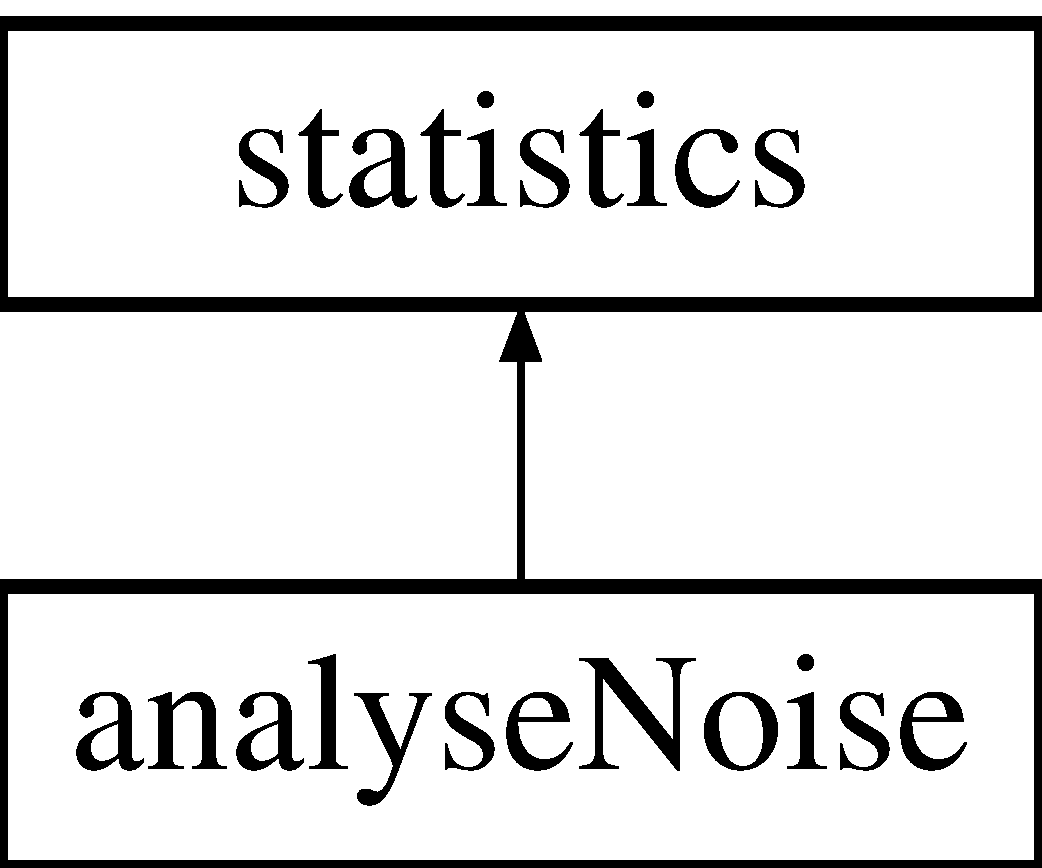
\includegraphics[height=2.000000cm]{classstatistics}
\end{center}
\end{figure}
\subsection*{Public Member Functions}
\begin{DoxyCompactItemize}
\item 
\hyperlink{classstatistics_a31d6750c3251c979f5c2d013984e1162}{statistics} ()
\item 
\hyperlink{classstatistics_a8cf720227802726be118712dc6616f94}{$\sim$statistics} ()
\item 
\hyperlink{classstatistics}{statistics} \hyperlink{classstatistics_a7e1f497f3e4780616e26bee24f30944d}{operator=} (\hyperlink{classstatistics}{statistics} zuw)
\item 
void \hyperlink{classstatistics_ae1c996db4172cc4f3011870565703949}{of} (unsigned short $\ast$data, int n)
\item 
void \hyperlink{classstatistics_adc449c82af5a264a3056553f79a23e4b}{of} (\hyperlink{classstatistics}{statistics} $\ast$stat, int n)
\item 
float \hyperlink{classstatistics_a7b484fdc49bf285ada28a5f422c503ac}{calc\-Mean} (unsigned short $\ast$data, int n)
\item 
unsigned short \hyperlink{classstatistics_a11bc27c277c69da2d9c9b73f02a50b84}{calc\-Min} (unsigned short $\ast$data, int n)
\item 
unsigned short \hyperlink{classstatistics_a25386f47edfa8c646ed6e6db836533c6}{calc\-Max} (unsigned short $\ast$data, int n)
\item 
float \hyperlink{classstatistics_a4765a751c416d896665eb38ccdccae85}{calc\-Variance} (unsigned short $\ast$data, int n)
\item 
void \hyperlink{classstatistics_ae75932ba711d0db5989bca5d8e7c13fd}{display} (F\-I\-L\-E $\ast$fout)
\item 
void \hyperlink{classstatistics_af09b9e0004c0df961422b58816a40c73}{set\-Mask} (unsigned short \hyperlink{classstatistics_a6cef2b7af0c9455ba4d7a3be62920d92}{mask})
\item 
void \hyperlink{classstatistics_a1c3f661ec160e9651baf2f5150e7176c}{add} (\hyperlink{classstatistics}{statistics} $\ast$stat)
\item 
void \hyperlink{classstatistics_ab509d6761e6556fd9c8ef9d056b7f9f0}{minus} (\hyperlink{classstatistics}{statistics} $\ast$stat)
\end{DoxyCompactItemize}
\subsection*{Public Attributes}
\begin{DoxyCompactItemize}
\item 
unsigned short \hyperlink{classstatistics_a9ddfcd7403d9a4ace35979ac3ad59fda}{min}
\item 
unsigned short \hyperlink{classstatistics_a46d65241f719918224650310f2fddecc}{max}
\item 
float \hyperlink{classstatistics_a5eacad512b051c45016ffeed7b35fe21}{mean}
\item 
float \hyperlink{classstatistics_a1397e63632ef6a3b87abfd35eff6485c}{variance}
\end{DoxyCompactItemize}
\subsection*{Private Attributes}
\begin{DoxyCompactItemize}
\item 
unsigned short \hyperlink{classstatistics_a6cef2b7af0c9455ba4d7a3be62920d92}{mask}
\end{DoxyCompactItemize}


\subsection{Detailed Description}
Provide statistics for a time series. The statistic is described by the minimum and maximum value, the mean value and the variance of the series. 

\subsection{Constructor \& Destructor Documentation}
\hypertarget{classstatistics_a31d6750c3251c979f5c2d013984e1162}{\index{statistics@{statistics}!statistics@{statistics}}
\index{statistics@{statistics}!statistics@{statistics}}
\subsubsection[{statistics}]{\setlength{\rightskip}{0pt plus 5cm}statistics\-::statistics (
\begin{DoxyParamCaption}
{}
\end{DoxyParamCaption}
)}}\label{classstatistics_a31d6750c3251c979f5c2d013984e1162}
\hypertarget{classstatistics_a8cf720227802726be118712dc6616f94}{\index{statistics@{statistics}!$\sim$statistics@{$\sim$statistics}}
\index{$\sim$statistics@{$\sim$statistics}!statistics@{statistics}}
\subsubsection[{$\sim$statistics}]{\setlength{\rightskip}{0pt plus 5cm}statistics\-::$\sim$statistics (
\begin{DoxyParamCaption}
{}
\end{DoxyParamCaption}
)}}\label{classstatistics_a8cf720227802726be118712dc6616f94}


\subsection{Member Function Documentation}
\hypertarget{classstatistics_a1c3f661ec160e9651baf2f5150e7176c}{\index{statistics@{statistics}!add@{add}}
\index{add@{add}!statistics@{statistics}}
\subsubsection[{add}]{\setlength{\rightskip}{0pt plus 5cm}void statistics\-::add (
\begin{DoxyParamCaption}
\item[{{\bf statistics} $\ast$}]{stat}
\end{DoxyParamCaption}
)}}\label{classstatistics_a1c3f661ec160e9651baf2f5150e7176c}
Add another statistical set \hypertarget{classstatistics_a25386f47edfa8c646ed6e6db836533c6}{\index{statistics@{statistics}!calc\-Max@{calc\-Max}}
\index{calc\-Max@{calc\-Max}!statistics@{statistics}}
\subsubsection[{calc\-Max}]{\setlength{\rightskip}{0pt plus 5cm}unsigned short statistics\-::calc\-Max (
\begin{DoxyParamCaption}
\item[{unsigned short $\ast$}]{data, }
\item[{int}]{n}
\end{DoxyParamCaption}
)}}\label{classstatistics_a25386f47edfa8c646ed6e6db836533c6}
\hypertarget{classstatistics_a7b484fdc49bf285ada28a5f422c503ac}{\index{statistics@{statistics}!calc\-Mean@{calc\-Mean}}
\index{calc\-Mean@{calc\-Mean}!statistics@{statistics}}
\subsubsection[{calc\-Mean}]{\setlength{\rightskip}{0pt plus 5cm}float statistics\-::calc\-Mean (
\begin{DoxyParamCaption}
\item[{unsigned short $\ast$}]{data, }
\item[{int}]{n}
\end{DoxyParamCaption}
)}}\label{classstatistics_a7b484fdc49bf285ada28a5f422c503ac}
\hypertarget{classstatistics_a11bc27c277c69da2d9c9b73f02a50b84}{\index{statistics@{statistics}!calc\-Min@{calc\-Min}}
\index{calc\-Min@{calc\-Min}!statistics@{statistics}}
\subsubsection[{calc\-Min}]{\setlength{\rightskip}{0pt plus 5cm}unsigned short statistics\-::calc\-Min (
\begin{DoxyParamCaption}
\item[{unsigned short $\ast$}]{data, }
\item[{int}]{n}
\end{DoxyParamCaption}
)}}\label{classstatistics_a11bc27c277c69da2d9c9b73f02a50b84}
\hypertarget{classstatistics_a4765a751c416d896665eb38ccdccae85}{\index{statistics@{statistics}!calc\-Variance@{calc\-Variance}}
\index{calc\-Variance@{calc\-Variance}!statistics@{statistics}}
\subsubsection[{calc\-Variance}]{\setlength{\rightskip}{0pt plus 5cm}float statistics\-::calc\-Variance (
\begin{DoxyParamCaption}
\item[{unsigned short $\ast$}]{data, }
\item[{int}]{n}
\end{DoxyParamCaption}
)}}\label{classstatistics_a4765a751c416d896665eb38ccdccae85}
\hypertarget{classstatistics_ae75932ba711d0db5989bca5d8e7c13fd}{\index{statistics@{statistics}!display@{display}}
\index{display@{display}!statistics@{statistics}}
\subsubsection[{display}]{\setlength{\rightskip}{0pt plus 5cm}void statistics\-::display (
\begin{DoxyParamCaption}
\item[{F\-I\-L\-E $\ast$}]{fout}
\end{DoxyParamCaption}
)}}\label{classstatistics_ae75932ba711d0db5989bca5d8e7c13fd}
\hypertarget{classstatistics_ab509d6761e6556fd9c8ef9d056b7f9f0}{\index{statistics@{statistics}!minus@{minus}}
\index{minus@{minus}!statistics@{statistics}}
\subsubsection[{minus}]{\setlength{\rightskip}{0pt plus 5cm}void statistics\-::minus (
\begin{DoxyParamCaption}
\item[{{\bf statistics} $\ast$}]{stat}
\end{DoxyParamCaption}
)}}\label{classstatistics_ab509d6761e6556fd9c8ef9d056b7f9f0}
Substract another statistical set \hypertarget{classstatistics_ae1c996db4172cc4f3011870565703949}{\index{statistics@{statistics}!of@{of}}
\index{of@{of}!statistics@{statistics}}
\subsubsection[{of}]{\setlength{\rightskip}{0pt plus 5cm}void statistics\-::of (
\begin{DoxyParamCaption}
\item[{unsigned short $\ast$}]{data, }
\item[{int}]{n}
\end{DoxyParamCaption}
)}}\label{classstatistics_ae1c996db4172cc4f3011870565703949}
Calculate the statistics a time series defined by n values of type unsigned short. \hypertarget{classstatistics_adc449c82af5a264a3056553f79a23e4b}{\index{statistics@{statistics}!of@{of}}
\index{of@{of}!statistics@{statistics}}
\subsubsection[{of}]{\setlength{\rightskip}{0pt plus 5cm}void statistics\-::of (
\begin{DoxyParamCaption}
\item[{{\bf statistics} $\ast$}]{stat, }
\item[{int}]{n}
\end{DoxyParamCaption}
)}}\label{classstatistics_adc449c82af5a264a3056553f79a23e4b}
Calculate the statistics of a time series that has been analysed in n segments of equal length \hypertarget{classstatistics_a7e1f497f3e4780616e26bee24f30944d}{\index{statistics@{statistics}!operator=@{operator=}}
\index{operator=@{operator=}!statistics@{statistics}}
\subsubsection[{operator=}]{\setlength{\rightskip}{0pt plus 5cm}{\bf statistics} statistics\-::operator= (
\begin{DoxyParamCaption}
\item[{{\bf statistics}}]{zuw}
\end{DoxyParamCaption}
)\hspace{0.3cm}{\ttfamily [inline]}}}\label{classstatistics_a7e1f497f3e4780616e26bee24f30944d}
\hypertarget{classstatistics_af09b9e0004c0df961422b58816a40c73}{\index{statistics@{statistics}!set\-Mask@{set\-Mask}}
\index{set\-Mask@{set\-Mask}!statistics@{statistics}}
\subsubsection[{set\-Mask}]{\setlength{\rightskip}{0pt plus 5cm}void statistics\-::set\-Mask (
\begin{DoxyParamCaption}
\item[{unsigned short}]{mask}
\end{DoxyParamCaption}
)\hspace{0.3cm}{\ttfamily [inline]}}}\label{classstatistics_af09b9e0004c0df961422b58816a40c73}
Set mask to select the data and remove possible flags 

\subsection{Member Data Documentation}
\hypertarget{classstatistics_a6cef2b7af0c9455ba4d7a3be62920d92}{\index{statistics@{statistics}!mask@{mask}}
\index{mask@{mask}!statistics@{statistics}}
\subsubsection[{mask}]{\setlength{\rightskip}{0pt plus 5cm}unsigned short statistics\-::mask\hspace{0.3cm}{\ttfamily [private]}}}\label{classstatistics_a6cef2b7af0c9455ba4d7a3be62920d92}
Mask for the data \hypertarget{classstatistics_a46d65241f719918224650310f2fddecc}{\index{statistics@{statistics}!max@{max}}
\index{max@{max}!statistics@{statistics}}
\subsubsection[{max}]{\setlength{\rightskip}{0pt plus 5cm}unsigned short statistics\-::max}}\label{classstatistics_a46d65241f719918224650310f2fddecc}
\hypertarget{classstatistics_a5eacad512b051c45016ffeed7b35fe21}{\index{statistics@{statistics}!mean@{mean}}
\index{mean@{mean}!statistics@{statistics}}
\subsubsection[{mean}]{\setlength{\rightskip}{0pt plus 5cm}float statistics\-::mean}}\label{classstatistics_a5eacad512b051c45016ffeed7b35fe21}
\hypertarget{classstatistics_a9ddfcd7403d9a4ace35979ac3ad59fda}{\index{statistics@{statistics}!min@{min}}
\index{min@{min}!statistics@{statistics}}
\subsubsection[{min}]{\setlength{\rightskip}{0pt plus 5cm}unsigned short statistics\-::min}}\label{classstatistics_a9ddfcd7403d9a4ace35979ac3ad59fda}
\hypertarget{classstatistics_a1397e63632ef6a3b87abfd35eff6485c}{\index{statistics@{statistics}!variance@{variance}}
\index{variance@{variance}!statistics@{statistics}}
\subsubsection[{variance}]{\setlength{\rightskip}{0pt plus 5cm}float statistics\-::variance}}\label{classstatistics_a1397e63632ef6a3b87abfd35eff6485c}


The documentation for this class was generated from the following files\-:\begin{DoxyCompactItemize}
\item 
/home/ntj/\-Development/phd/kitcube-\/tools/src/akutil/\hyperlink{statistics_8h}{statistics.\-h}\item 
/home/ntj/\-Development/phd/kitcube-\/tools/src/akutil/\hyperlink{statistics_8cpp}{statistics.\-cpp}\end{DoxyCompactItemize}

\hypertarget{classSysLog}{\section{Sys\-Log Class Reference}
\label{classSysLog}\index{Sys\-Log@{Sys\-Log}}
}


{\ttfamily \#include $<$syslog.\-h$>$}

Inheritance diagram for Sys\-Log\-:\begin{figure}[H]
\begin{center}
\leavevmode
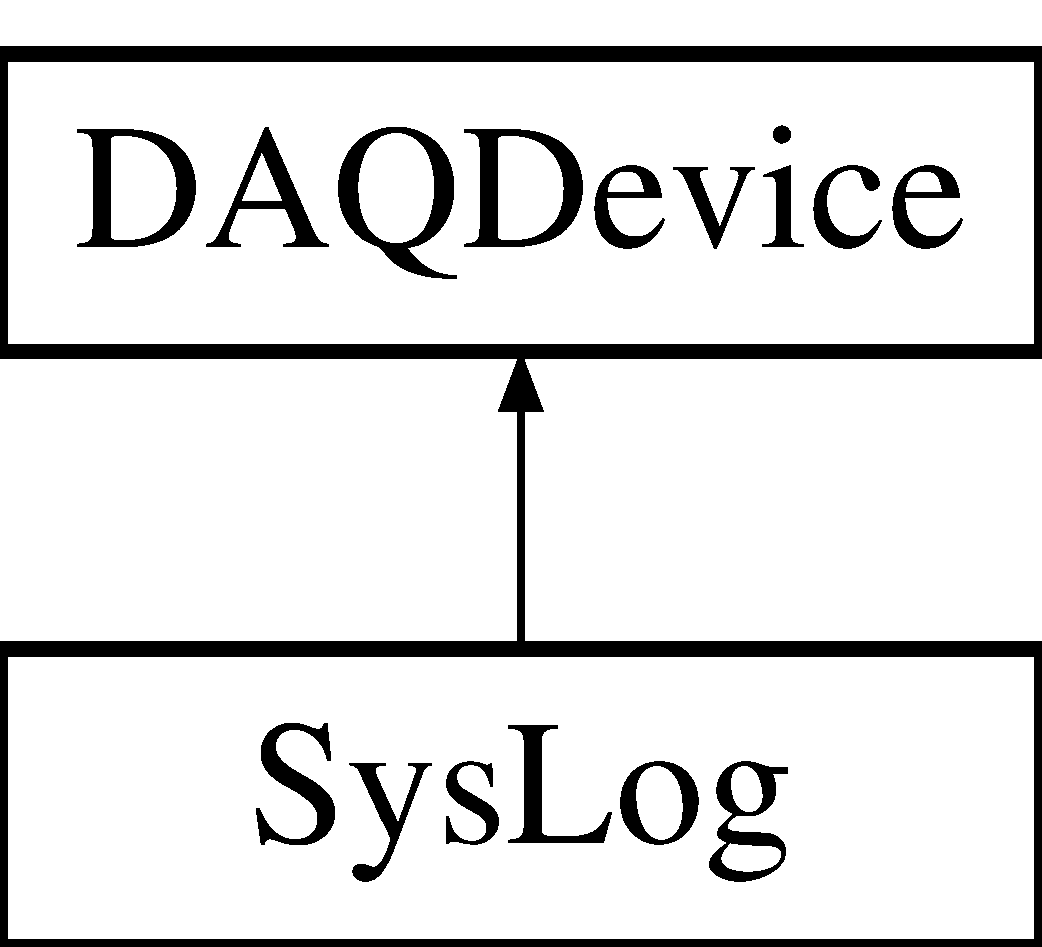
\includegraphics[height=2.000000cm]{classSysLog}
\end{center}
\end{figure}
\subsection*{Public Member Functions}
\begin{DoxyCompactItemize}
\item 
\hyperlink{classSysLog_a06c2e3fd7b6e5dca3cfbcc0b913c6e75}{Sys\-Log} ()
\item 
\hyperlink{classSysLog_ad5b4de59a0e4c4be08430073d43fee5c}{$\sim$\-Sys\-Log} ()
\item 
void \hyperlink{classSysLog_a7a68d2e9cb7ab67ba5fac6a842ddf9ed}{set\-Config\-Defaults} ()
\item 
void \hyperlink{classSysLog_a1a6772be111f471271fce194955e69f8}{set\-App\-Id} (int \hyperlink{classDAQDevice_a2f0b3d2e531be7f5d06f47a4753d35bd}{app\-Id})
\item 
void \hyperlink{classSysLog_a6b6900287d6fca70de47fb11c3b4877d}{set\-N\-Data} (int n)
\item 
void \hyperlink{classSysLog_a6f7aa19cdb467d56ea0af13b3dd7a01d}{set\-Config} (int ch, const char $\ast$name)
\item 
void \hyperlink{classSysLog_aeb21706d3a9353ab083662bae6430a3d}{update\-Timestamp} (struct timeval $\ast$t)
\item 
void \hyperlink{classSysLog_a0b61756d28ad5d54344ecf66031b6407}{update\-Data} (int ch, float data)
\end{DoxyCompactItemize}
\subsection*{Additional Inherited Members}


\subsection{Detailed Description}
Implementation for the performance module.

Alternatively also a file could be defined. If the main tasks writes all performance data to a file. the performance module would operate like all the other modules. 

\subsection{Constructor \& Destructor Documentation}
\hypertarget{classSysLog_a06c2e3fd7b6e5dca3cfbcc0b913c6e75}{\index{Sys\-Log@{Sys\-Log}!Sys\-Log@{Sys\-Log}}
\index{Sys\-Log@{Sys\-Log}!SysLog@{Sys\-Log}}
\subsubsection[{Sys\-Log}]{\setlength{\rightskip}{0pt plus 5cm}Sys\-Log\-::\-Sys\-Log (
\begin{DoxyParamCaption}
{}
\end{DoxyParamCaption}
)}}\label{classSysLog_a06c2e3fd7b6e5dca3cfbcc0b913c6e75}
\hypertarget{classSysLog_ad5b4de59a0e4c4be08430073d43fee5c}{\index{Sys\-Log@{Sys\-Log}!$\sim$\-Sys\-Log@{$\sim$\-Sys\-Log}}
\index{$\sim$\-Sys\-Log@{$\sim$\-Sys\-Log}!SysLog@{Sys\-Log}}
\subsubsection[{$\sim$\-Sys\-Log}]{\setlength{\rightskip}{0pt plus 5cm}Sys\-Log\-::$\sim$\-Sys\-Log (
\begin{DoxyParamCaption}
{}
\end{DoxyParamCaption}
)}}\label{classSysLog_ad5b4de59a0e4c4be08430073d43fee5c}


\subsection{Member Function Documentation}
\hypertarget{classSysLog_a1a6772be111f471271fce194955e69f8}{\index{Sys\-Log@{Sys\-Log}!set\-App\-Id@{set\-App\-Id}}
\index{set\-App\-Id@{set\-App\-Id}!SysLog@{Sys\-Log}}
\subsubsection[{set\-App\-Id}]{\setlength{\rightskip}{0pt plus 5cm}void Sys\-Log\-::set\-App\-Id (
\begin{DoxyParamCaption}
\item[{int}]{app\-Id}
\end{DoxyParamCaption}
)\hspace{0.3cm}{\ttfamily [virtual]}}}\label{classSysLog_a1a6772be111f471271fce194955e69f8}
Read parameter from inifile Select the module id according to the application id 

Reimplemented from \hyperlink{classDAQDevice_a42934eca41ab337dc5874e9e70ba1fab}{D\-A\-Q\-Device}.

\hypertarget{classSysLog_a6f7aa19cdb467d56ea0af13b3dd7a01d}{\index{Sys\-Log@{Sys\-Log}!set\-Config@{set\-Config}}
\index{set\-Config@{set\-Config}!SysLog@{Sys\-Log}}
\subsubsection[{set\-Config}]{\setlength{\rightskip}{0pt plus 5cm}void Sys\-Log\-::set\-Config (
\begin{DoxyParamCaption}
\item[{int}]{ch, }
\item[{const char $\ast$}]{name}
\end{DoxyParamCaption}
)}}\label{classSysLog_a6f7aa19cdb467d56ea0af13b3dd7a01d}
Initialize the data set. A channel is defined by the name and the data type. Available data types are 0 int and 1 float \hypertarget{classSysLog_a7a68d2e9cb7ab67ba5fac6a842ddf9ed}{\index{Sys\-Log@{Sys\-Log}!set\-Config\-Defaults@{set\-Config\-Defaults}}
\index{set\-Config\-Defaults@{set\-Config\-Defaults}!SysLog@{Sys\-Log}}
\subsubsection[{set\-Config\-Defaults}]{\setlength{\rightskip}{0pt plus 5cm}void Sys\-Log\-::set\-Config\-Defaults (
\begin{DoxyParamCaption}
{}
\end{DoxyParamCaption}
)\hspace{0.3cm}{\ttfamily [virtual]}}}\label{classSysLog_a7a68d2e9cb7ab67ba5fac6a842ddf9ed}
Set default configuration 

Reimplemented from \hyperlink{classDAQDevice_a7685cec80865752cc0ef3ab49c6c2277}{D\-A\-Q\-Device}.

\hypertarget{classSysLog_a6b6900287d6fca70de47fb11c3b4877d}{\index{Sys\-Log@{Sys\-Log}!set\-N\-Data@{set\-N\-Data}}
\index{set\-N\-Data@{set\-N\-Data}!SysLog@{Sys\-Log}}
\subsubsection[{set\-N\-Data}]{\setlength{\rightskip}{0pt plus 5cm}void Sys\-Log\-::set\-N\-Data (
\begin{DoxyParamCaption}
\item[{int}]{n}
\end{DoxyParamCaption}
)}}\label{classSysLog_a6b6900287d6fca70de47fb11c3b4877d}
Define the number arguments. This function will also alocate memory \hypertarget{classSysLog_a0b61756d28ad5d54344ecf66031b6407}{\index{Sys\-Log@{Sys\-Log}!update\-Data@{update\-Data}}
\index{update\-Data@{update\-Data}!SysLog@{Sys\-Log}}
\subsubsection[{update\-Data}]{\setlength{\rightskip}{0pt plus 5cm}void Sys\-Log\-::update\-Data (
\begin{DoxyParamCaption}
\item[{int}]{ch, }
\item[{float}]{data}
\end{DoxyParamCaption}
)}}\label{classSysLog_a0b61756d28ad5d54344ecf66031b6407}
\hypertarget{classSysLog_aeb21706d3a9353ab083662bae6430a3d}{\index{Sys\-Log@{Sys\-Log}!update\-Timestamp@{update\-Timestamp}}
\index{update\-Timestamp@{update\-Timestamp}!SysLog@{Sys\-Log}}
\subsubsection[{update\-Timestamp}]{\setlength{\rightskip}{0pt plus 5cm}void Sys\-Log\-::update\-Timestamp (
\begin{DoxyParamCaption}
\item[{struct timeval $\ast$}]{t}
\end{DoxyParamCaption}
)}}\label{classSysLog_aeb21706d3a9353ab083662bae6430a3d}
Update data set 

The documentation for this class was generated from the following files\-:\begin{DoxyCompactItemize}
\item 
/home/ntj/\-Development/phd/kitcube-\/tools/src/kitcube-\/devices/\hyperlink{syslog_8h}{syslog.\-h}\item 
/home/ntj/\-Development/phd/kitcube-\/tools/src/kitcube-\/devices/\hyperlink{syslog_8cpp}{syslog.\-cpp}\end{DoxyCompactItemize}

\hypertarget{classUnsignedInt64}{\section{Unsigned\-Int64 Class Reference}
\label{classUnsignedInt64}\index{Unsigned\-Int64@{Unsigned\-Int64}}
}


{\ttfamily \#include $<$unsignedint64.\-h$>$}

\subsection*{Public Member Functions}
\begin{DoxyCompactItemize}
\item 
\hyperlink{classUnsignedInt64_ad45cee6b995cad3062c906c5ed2705d9}{Unsigned\-Int64} ()
\item 
\hyperlink{classUnsignedInt64_a2767927a925ab2e7186c863f16043a9d}{$\sim$\-Unsigned\-Int64} ()
\item 
void \hyperlink{classUnsignedInt64_af813efd90a8e9e1fc89d9274dfc874db}{add} (unsigned long $\ast$sum1, unsigned long $\ast$sum2)
\item 
void \hyperlink{classUnsignedInt64_a08a0cdd031c49ca9165e77dd92ff5cf5}{add} (unsigned long $\ast$sum1, unsigned long sum2)
\item 
void \hyperlink{classUnsignedInt64_af8da78cf70fa21dc3003c4779259d006}{mult} (unsigned long $\ast$prod1, unsigned long $\ast$prod2)
\item 
void \hyperlink{classUnsignedInt64_a9f20d16d3d75f6e646be3809638a088d}{mult} (unsigned long $\ast$prod1, unsigned short prod2)
\item 
void \hyperlink{classUnsignedInt64_aa1a72d942a20576932f1a1329b0d9df6}{div} (unsigned long $\ast$div1, unsigned short div2)
\item 
unsigned short \hyperlink{classUnsignedInt64_a17ba5f97b8bd42a4555dbaf53a6bd269}{mod} (unsigned long $\ast$div1, unsigned short div2)
\item 
int \hyperlink{classUnsignedInt64_a61d831da583bf56ac44c32f02dc5afee}{test} (int level=0)
\item 
unsigned long $\ast$ \hyperlink{classUnsignedInt64_a577122e70df0f33191add0d9305771cb}{get} ()
\end{DoxyCompactItemize}
\subsection*{Private Attributes}
\begin{DoxyCompactItemize}
\item 
unsigned long \hyperlink{classUnsignedInt64_a34f0d86cf4dd2f0523e1c844d169eaa9}{data} \mbox{[}2\mbox{]}
\end{DoxyCompactItemize}


\subsection{Detailed Description}
64bit data type.

\begin{DoxyRefDesc}{Todo}
\item[\hyperlink{todo__todo000007}{Todo}]Implement operators to make the handling comparable to standard data types \end{DoxyRefDesc}


\subsection{Constructor \& Destructor Documentation}
\hypertarget{classUnsignedInt64_ad45cee6b995cad3062c906c5ed2705d9}{\index{Unsigned\-Int64@{Unsigned\-Int64}!Unsigned\-Int64@{Unsigned\-Int64}}
\index{Unsigned\-Int64@{Unsigned\-Int64}!UnsignedInt64@{Unsigned\-Int64}}
\subsubsection[{Unsigned\-Int64}]{\setlength{\rightskip}{0pt plus 5cm}Unsigned\-Int64\-::\-Unsigned\-Int64 (
\begin{DoxyParamCaption}
{}
\end{DoxyParamCaption}
)}}\label{classUnsignedInt64_ad45cee6b995cad3062c906c5ed2705d9}
\hypertarget{classUnsignedInt64_a2767927a925ab2e7186c863f16043a9d}{\index{Unsigned\-Int64@{Unsigned\-Int64}!$\sim$\-Unsigned\-Int64@{$\sim$\-Unsigned\-Int64}}
\index{$\sim$\-Unsigned\-Int64@{$\sim$\-Unsigned\-Int64}!UnsignedInt64@{Unsigned\-Int64}}
\subsubsection[{$\sim$\-Unsigned\-Int64}]{\setlength{\rightskip}{0pt plus 5cm}Unsigned\-Int64\-::$\sim$\-Unsigned\-Int64 (
\begin{DoxyParamCaption}
{}
\end{DoxyParamCaption}
)}}\label{classUnsignedInt64_a2767927a925ab2e7186c863f16043a9d}


\subsection{Member Function Documentation}
\hypertarget{classUnsignedInt64_af813efd90a8e9e1fc89d9274dfc874db}{\index{Unsigned\-Int64@{Unsigned\-Int64}!add@{add}}
\index{add@{add}!UnsignedInt64@{Unsigned\-Int64}}
\subsubsection[{add}]{\setlength{\rightskip}{0pt plus 5cm}void Unsigned\-Int64\-::add (
\begin{DoxyParamCaption}
\item[{unsigned long $\ast$}]{sum1, }
\item[{unsigned long $\ast$}]{sum2}
\end{DoxyParamCaption}
)}}\label{classUnsignedInt64_af813efd90a8e9e1fc89d9274dfc874db}
Add a 64 bit value to another \hypertarget{classUnsignedInt64_a08a0cdd031c49ca9165e77dd92ff5cf5}{\index{Unsigned\-Int64@{Unsigned\-Int64}!add@{add}}
\index{add@{add}!UnsignedInt64@{Unsigned\-Int64}}
\subsubsection[{add}]{\setlength{\rightskip}{0pt plus 5cm}void Unsigned\-Int64\-::add (
\begin{DoxyParamCaption}
\item[{unsigned long $\ast$}]{sum1, }
\item[{unsigned long}]{sum2}
\end{DoxyParamCaption}
)}}\label{classUnsignedInt64_a08a0cdd031c49ca9165e77dd92ff5cf5}
Add a 64 bit value to another \hypertarget{classUnsignedInt64_aa1a72d942a20576932f1a1329b0d9df6}{\index{Unsigned\-Int64@{Unsigned\-Int64}!div@{div}}
\index{div@{div}!UnsignedInt64@{Unsigned\-Int64}}
\subsubsection[{div}]{\setlength{\rightskip}{0pt plus 5cm}void Unsigned\-Int64\-::div (
\begin{DoxyParamCaption}
\item[{unsigned long $\ast$}]{div1, }
\item[{unsigned short}]{div2}
\end{DoxyParamCaption}
)}}\label{classUnsignedInt64_aa1a72d942a20576932f1a1329b0d9df6}
Divide a 64bit value by a 32bit value \hypertarget{classUnsignedInt64_a577122e70df0f33191add0d9305771cb}{\index{Unsigned\-Int64@{Unsigned\-Int64}!get@{get}}
\index{get@{get}!UnsignedInt64@{Unsigned\-Int64}}
\subsubsection[{get}]{\setlength{\rightskip}{0pt plus 5cm}unsigned long $\ast$ Unsigned\-Int64\-::get (
\begin{DoxyParamCaption}
{}
\end{DoxyParamCaption}
)}}\label{classUnsignedInt64_a577122e70df0f33191add0d9305771cb}
Get pointer to the data \hypertarget{classUnsignedInt64_a17ba5f97b8bd42a4555dbaf53a6bd269}{\index{Unsigned\-Int64@{Unsigned\-Int64}!mod@{mod}}
\index{mod@{mod}!UnsignedInt64@{Unsigned\-Int64}}
\subsubsection[{mod}]{\setlength{\rightskip}{0pt plus 5cm}unsigned short Unsigned\-Int64\-::mod (
\begin{DoxyParamCaption}
\item[{unsigned long $\ast$}]{div1, }
\item[{unsigned short}]{div2}
\end{DoxyParamCaption}
)}}\label{classUnsignedInt64_a17ba5f97b8bd42a4555dbaf53a6bd269}
Calculate modulo operations on a 64 number \hypertarget{classUnsignedInt64_af8da78cf70fa21dc3003c4779259d006}{\index{Unsigned\-Int64@{Unsigned\-Int64}!mult@{mult}}
\index{mult@{mult}!UnsignedInt64@{Unsigned\-Int64}}
\subsubsection[{mult}]{\setlength{\rightskip}{0pt plus 5cm}void Unsigned\-Int64\-::mult (
\begin{DoxyParamCaption}
\item[{unsigned long $\ast$}]{prod1, }
\item[{unsigned long $\ast$}]{prod2}
\end{DoxyParamCaption}
)}}\label{classUnsignedInt64_af8da78cf70fa21dc3003c4779259d006}
Multiply two 64 bit values \hypertarget{classUnsignedInt64_a9f20d16d3d75f6e646be3809638a088d}{\index{Unsigned\-Int64@{Unsigned\-Int64}!mult@{mult}}
\index{mult@{mult}!UnsignedInt64@{Unsigned\-Int64}}
\subsubsection[{mult}]{\setlength{\rightskip}{0pt plus 5cm}void Unsigned\-Int64\-::mult (
\begin{DoxyParamCaption}
\item[{unsigned long $\ast$}]{prod1, }
\item[{unsigned short}]{prod2}
\end{DoxyParamCaption}
)}}\label{classUnsignedInt64_a9f20d16d3d75f6e646be3809638a088d}
Multiply a 64bit value with a 16bit value \hypertarget{classUnsignedInt64_a61d831da583bf56ac44c32f02dc5afee}{\index{Unsigned\-Int64@{Unsigned\-Int64}!test@{test}}
\index{test@{test}!UnsignedInt64@{Unsigned\-Int64}}
\subsubsection[{test}]{\setlength{\rightskip}{0pt plus 5cm}int Unsigned\-Int64\-::test (
\begin{DoxyParamCaption}
\item[{int}]{level = {\ttfamily 0}}
\end{DoxyParamCaption}
)}}\label{classUnsignedInt64_a61d831da583bf56ac44c32f02dc5afee}
Test the 64bit operations 

\subsection{Member Data Documentation}
\hypertarget{classUnsignedInt64_a34f0d86cf4dd2f0523e1c844d169eaa9}{\index{Unsigned\-Int64@{Unsigned\-Int64}!data@{data}}
\index{data@{data}!UnsignedInt64@{Unsigned\-Int64}}
\subsubsection[{data}]{\setlength{\rightskip}{0pt plus 5cm}unsigned long Unsigned\-Int64\-::data\mbox{[}2\mbox{]}\hspace{0.3cm}{\ttfamily [private]}}}\label{classUnsignedInt64_a34f0d86cf4dd2f0523e1c844d169eaa9}
64bit data 

The documentation for this class was generated from the following files\-:\begin{DoxyCompactItemize}
\item 
/home/ntj/\-Development/phd/kitcube-\/tools/src/akutil/\hyperlink{unsignedint64_8h}{unsignedint64.\-h}\item 
/home/ntj/\-Development/phd/kitcube-\/tools/src/akutil/\hyperlink{unsignedint64_8cpp}{unsignedint64.\-cpp}\end{DoxyCompactItemize}

\hypertarget{classWGCommand}{\section{W\-G\-Command Class Reference}
\label{classWGCommand}\index{W\-G\-Command@{W\-G\-Command}}
}


{\ttfamily \#include $<$wgcommand.\-h$>$}

\subsection*{Public Member Functions}
\begin{DoxyCompactItemize}
\item 
\hyperlink{classWGCommand_a9b5240b14844df1f1ddbcd1d7fd002dc}{W\-G\-Command} ()
\item 
\hyperlink{classWGCommand_a1476b046244df1ef8b6de59ace33d6e2}{$\sim$\-W\-G\-Command} ()
\item 
void \hyperlink{classWGCommand_a131dd16defc78995a469b076b2970b41}{open\-Device} (const char $\ast$\hyperlink{classWGCommand_ad87845443f95cc2d0fb33299a13de26b}{device}=\char`\"{}/dev/tty\-S0\char`\"{})
\item 
void \hyperlink{classWGCommand_a1ad4abc6d61d3816ac9e038d11bef5e0}{close\-Device} ()
\item 
void \hyperlink{classWGCommand_a4590108efb24e34b24300567c36c23d0}{send\-Cmd} (unsigned char $\ast$cmd, unsigned char $\ast$ack)
\item 
int \hyperlink{classWGCommand_a46dca886ad75d9c742272273d5c9e7e1}{get\-Parameter} (char cmd\-Id)
\item 
void \hyperlink{classWGCommand_a29b808745bdaa0f1687d856659479938}{set\-Parameter} (char cmd\-Id, int par1=0, int par2=0)
\item 
void \hyperlink{classWGCommand_a98093256ad22ec30afb3e2e2e3616fe1}{set\-Debug} (int \hyperlink{classWGCommand_a2e554051536b4ee562c3ccd49071e0be}{debug})
\item 
void \hyperlink{classWGCommand_af8bc46cc6907f71ac248fdde0401d739}{get\-Type} (int $\ast$model, int $\ast$n\-Channel=0, int $\ast$morph=0)
\item 
int \hyperlink{classWGCommand_ac4a1887b09ed43f41b1124f9361dc202}{get\-Version} (char $\ast$version)
\item 
void \hyperlink{classWGCommand_a004a8da3605eaa045549f8307ef68632}{set\-Defaults} ()
\item 
void \hyperlink{classWGCommand_a5b25fc2d24d24e9e02808d2a95639059}{set\-Mode} (int mode)
\item 
int \hyperlink{classWGCommand_a9d137d3e0c5c82713dd558d05129f444}{get\-Mode} ()
\item 
void \hyperlink{classWGCommand_a3e6be43025cb18a6b56e1fd0c5bbd69b}{set\-Amplitude} (double amplitude)
\item 
double \hyperlink{classWGCommand_a4713ae94de47c9ecd57949f07b0cc151}{get\-Amplitude} ()
\item 
void \hyperlink{classWGCommand_a5b47333d3124ca82072f03aaa9d65b80}{set\-Frequency} (double frequency)
\item 
double \hyperlink{classWGCommand_ae580772a1332d8d437a1fc1ab9d6fc55}{get\-Frequency} ()
\item 
void \hyperlink{classWGCommand_a73126eeabfd108feb1c547e44d43cb8d}{set\-Offset} (double offset)
\item 
double \hyperlink{classWGCommand_a75cff5b6f1cea081004259d898543926}{get\-Offset} ()
\item 
void \hyperlink{classWGCommand_aa30bbb9753ddc47a5fd6b51f177950ff}{set\-Offset\-Mode} (int mode)
\item 
int \hyperlink{classWGCommand_a81acd94c40932d37abd0ec8614556329}{get\-Offset\-Mode} ()
\item 
void \hyperlink{classWGCommand_aa47567ce9d687d01a72d0506c88e79cb}{set\-Filter\-Mode} (int mode)
\item 
int \hyperlink{classWGCommand_ad82bd84a6104712acf8a47f4491ac7bb}{get\-Filter\-Mode} ()
\item 
void \hyperlink{classWGCommand_a47122b52d714a3ef13858c08afe880f1}{set\-Duty\-Cycle} (int dutycycle)
\item 
int \hyperlink{classWGCommand_a1b5461eccc1d174ff05c3f46e638327b}{get\-Duty\-Cycle} ()
\item 
void \hyperlink{classWGCommand_ac1431f39952eae310f2ae7990473a55a}{set\-Sync\-Position} (int pos)
\item 
int \hyperlink{classWGCommand_a04bc036b7e0ad58b4d0844d515c2e885}{get\-Sync\-Position} ()
\item 
void \hyperlink{classWGCommand_a33312bd06b15c1e3cbc4d50830e5cc52}{set\-Modulation} (int mode)
\item 
int \hyperlink{classWGCommand_aef97c0aa47ea2495abcfcbbfa9d991f4}{get\-Modulation} ()
\item 
void \hyperlink{classWGCommand_aa317f017e752e12d72d7237e893bee4e}{set\-Trigger\-Mode} ()
\item 
int \hyperlink{classWGCommand_ab80c1d114f82ebe000ae15e465cdade6}{get\-Trigger\-Mode} ()
\item 
void \hyperlink{classWGCommand_a23bf43da881800b384e3d6ef88747187}{set\-Clock} (int source)
\item 
int \hyperlink{classWGCommand_a43b9e42d1eb6de888ec4555271207073}{get\-Clock} ()
\item 
void \hyperlink{classWGCommand_a7bfa70c2e89d9face4c826fd3f788c4b}{set\-Wave\-Form} (int mode)
\item 
int \hyperlink{classWGCommand_a13f47f4516c2b2d0f306d7b191d285cc}{get\-Wave\-Form} ()
\item 
void \hyperlink{classWGCommand_a2e9c8acc3d2064530cb42a437a10e4f5}{set\-Gain} (int \hyperlink{classWGCommand_a48891c9df29d1988fe828bb18906bf89}{gain})
\item 
int \hyperlink{classWGCommand_a99c983f98ac8966616850595561270e7}{get\-Gain} ()
\item 
double \hyperlink{classWGCommand_a135690529a0aa3acc784db2bb6063857}{exp10} (double exp)
\end{DoxyCompactItemize}
\subsection*{Private Attributes}
\begin{DoxyCompactItemize}
\item 
int \hyperlink{classWGCommand_a2e554051536b4ee562c3ccd49071e0be}{debug}
\item 
std\-::string \hyperlink{classWGCommand_ad87845443f95cc2d0fb33299a13de26b}{device}
\item 
int \hyperlink{classWGCommand_a6f4376a362141d0f49efe521156d838b}{fd}
\item 
struct termios \hyperlink{classWGCommand_a82bdfe137d61716e32ffd2b7dd69d9e2}{wg\-Tio}
\item 
struct termios \hyperlink{classWGCommand_aa87ce887cb2d9c80cfe87efd84fa4362}{buffered\-Tio}
\item 
char \hyperlink{classWGCommand_a05dbd3492228efc134722a23daff633f}{last\-Ack} \mbox{[}7\mbox{]}
\item 
double \hyperlink{classWGCommand_a48891c9df29d1988fe828bb18906bf89}{gain}
\end{DoxyCompactItemize}


\subsection{Detailed Description}
Implementation of the W\-G Command interface defined by Mair \& Rohner O\-E\-G (M\&R Systems, www.\-mrsys.\-at) for their waveform generators.

Tested with waveform generator W\-G-\/1220.

\begin{DoxyRefDesc}{Todo}
\item[\hyperlink{todo__todo000008}{Todo}]Implement timeout waiting for the device 

Implement the missing commands\end{DoxyRefDesc}


\subsection{Constructor \& Destructor Documentation}
\hypertarget{classWGCommand_a9b5240b14844df1f1ddbcd1d7fd002dc}{\index{W\-G\-Command@{W\-G\-Command}!W\-G\-Command@{W\-G\-Command}}
\index{W\-G\-Command@{W\-G\-Command}!WGCommand@{W\-G\-Command}}
\subsubsection[{W\-G\-Command}]{\setlength{\rightskip}{0pt plus 5cm}W\-G\-Command\-::\-W\-G\-Command (
\begin{DoxyParamCaption}
{}
\end{DoxyParamCaption}
)}}\label{classWGCommand_a9b5240b14844df1f1ddbcd1d7fd002dc}
\hypertarget{classWGCommand_a1476b046244df1ef8b6de59ace33d6e2}{\index{W\-G\-Command@{W\-G\-Command}!$\sim$\-W\-G\-Command@{$\sim$\-W\-G\-Command}}
\index{$\sim$\-W\-G\-Command@{$\sim$\-W\-G\-Command}!WGCommand@{W\-G\-Command}}
\subsubsection[{$\sim$\-W\-G\-Command}]{\setlength{\rightskip}{0pt plus 5cm}W\-G\-Command\-::$\sim$\-W\-G\-Command (
\begin{DoxyParamCaption}
{}
\end{DoxyParamCaption}
)}}\label{classWGCommand_a1476b046244df1ef8b6de59ace33d6e2}


\subsection{Member Function Documentation}
\hypertarget{classWGCommand_a1ad4abc6d61d3816ac9e038d11bef5e0}{\index{W\-G\-Command@{W\-G\-Command}!close\-Device@{close\-Device}}
\index{close\-Device@{close\-Device}!WGCommand@{W\-G\-Command}}
\subsubsection[{close\-Device}]{\setlength{\rightskip}{0pt plus 5cm}void W\-G\-Command\-::close\-Device (
\begin{DoxyParamCaption}
{}
\end{DoxyParamCaption}
)}}\label{classWGCommand_a1ad4abc6d61d3816ac9e038d11bef5e0}
Close device. Restore the parameters of the device \hypertarget{classWGCommand_a135690529a0aa3acc784db2bb6063857}{\index{W\-G\-Command@{W\-G\-Command}!exp10@{exp10}}
\index{exp10@{exp10}!WGCommand@{W\-G\-Command}}
\subsubsection[{exp10}]{\setlength{\rightskip}{0pt plus 5cm}double W\-G\-Command\-::exp10 (
\begin{DoxyParamCaption}
\item[{double}]{exp}
\end{DoxyParamCaption}
)}}\label{classWGCommand_a135690529a0aa3acc784db2bb6063857}
Calculate 10 power exp \hypertarget{classWGCommand_a4713ae94de47c9ecd57949f07b0cc151}{\index{W\-G\-Command@{W\-G\-Command}!get\-Amplitude@{get\-Amplitude}}
\index{get\-Amplitude@{get\-Amplitude}!WGCommand@{W\-G\-Command}}
\subsubsection[{get\-Amplitude}]{\setlength{\rightskip}{0pt plus 5cm}double W\-G\-Command\-::get\-Amplitude (
\begin{DoxyParamCaption}
{}
\end{DoxyParamCaption}
)}}\label{classWGCommand_a4713ae94de47c9ecd57949f07b0cc151}
Get amplitude in m\-V \hypertarget{classWGCommand_a43b9e42d1eb6de888ec4555271207073}{\index{W\-G\-Command@{W\-G\-Command}!get\-Clock@{get\-Clock}}
\index{get\-Clock@{get\-Clock}!WGCommand@{W\-G\-Command}}
\subsubsection[{get\-Clock}]{\setlength{\rightskip}{0pt plus 5cm}int W\-G\-Command\-::get\-Clock (
\begin{DoxyParamCaption}
{}
\end{DoxyParamCaption}
)}}\label{classWGCommand_a43b9e42d1eb6de888ec4555271207073}
Get clock source \hypertarget{classWGCommand_a1b5461eccc1d174ff05c3f46e638327b}{\index{W\-G\-Command@{W\-G\-Command}!get\-Duty\-Cycle@{get\-Duty\-Cycle}}
\index{get\-Duty\-Cycle@{get\-Duty\-Cycle}!WGCommand@{W\-G\-Command}}
\subsubsection[{get\-Duty\-Cycle}]{\setlength{\rightskip}{0pt plus 5cm}int W\-G\-Command\-::get\-Duty\-Cycle (
\begin{DoxyParamCaption}
{}
\end{DoxyParamCaption}
)}}\label{classWGCommand_a1b5461eccc1d174ff05c3f46e638327b}
Get duty cycle \hypertarget{classWGCommand_ad82bd84a6104712acf8a47f4491ac7bb}{\index{W\-G\-Command@{W\-G\-Command}!get\-Filter\-Mode@{get\-Filter\-Mode}}
\index{get\-Filter\-Mode@{get\-Filter\-Mode}!WGCommand@{W\-G\-Command}}
\subsubsection[{get\-Filter\-Mode}]{\setlength{\rightskip}{0pt plus 5cm}int W\-G\-Command\-::get\-Filter\-Mode (
\begin{DoxyParamCaption}
{}
\end{DoxyParamCaption}
)}}\label{classWGCommand_ad82bd84a6104712acf8a47f4491ac7bb}
Get filter mode \hypertarget{classWGCommand_ae580772a1332d8d437a1fc1ab9d6fc55}{\index{W\-G\-Command@{W\-G\-Command}!get\-Frequency@{get\-Frequency}}
\index{get\-Frequency@{get\-Frequency}!WGCommand@{W\-G\-Command}}
\subsubsection[{get\-Frequency}]{\setlength{\rightskip}{0pt plus 5cm}double W\-G\-Command\-::get\-Frequency (
\begin{DoxyParamCaption}
{}
\end{DoxyParamCaption}
)}}\label{classWGCommand_ae580772a1332d8d437a1fc1ab9d6fc55}
Get freqency in Hz \hypertarget{classWGCommand_a99c983f98ac8966616850595561270e7}{\index{W\-G\-Command@{W\-G\-Command}!get\-Gain@{get\-Gain}}
\index{get\-Gain@{get\-Gain}!WGCommand@{W\-G\-Command}}
\subsubsection[{get\-Gain}]{\setlength{\rightskip}{0pt plus 5cm}int W\-G\-Command\-::get\-Gain (
\begin{DoxyParamCaption}
{}
\end{DoxyParamCaption}
)}}\label{classWGCommand_a99c983f98ac8966616850595561270e7}
Get gain \hypertarget{classWGCommand_a9d137d3e0c5c82713dd558d05129f444}{\index{W\-G\-Command@{W\-G\-Command}!get\-Mode@{get\-Mode}}
\index{get\-Mode@{get\-Mode}!WGCommand@{W\-G\-Command}}
\subsubsection[{get\-Mode}]{\setlength{\rightskip}{0pt plus 5cm}int W\-G\-Command\-::get\-Mode (
\begin{DoxyParamCaption}
{}
\end{DoxyParamCaption}
)}}\label{classWGCommand_a9d137d3e0c5c82713dd558d05129f444}
Request mode (0 = remote/ 1= local) \hypertarget{classWGCommand_aef97c0aa47ea2495abcfcbbfa9d991f4}{\index{W\-G\-Command@{W\-G\-Command}!get\-Modulation@{get\-Modulation}}
\index{get\-Modulation@{get\-Modulation}!WGCommand@{W\-G\-Command}}
\subsubsection[{get\-Modulation}]{\setlength{\rightskip}{0pt plus 5cm}int W\-G\-Command\-::get\-Modulation (
\begin{DoxyParamCaption}
{}
\end{DoxyParamCaption}
)}}\label{classWGCommand_aef97c0aa47ea2495abcfcbbfa9d991f4}
Get modulation type \hypertarget{classWGCommand_a75cff5b6f1cea081004259d898543926}{\index{W\-G\-Command@{W\-G\-Command}!get\-Offset@{get\-Offset}}
\index{get\-Offset@{get\-Offset}!WGCommand@{W\-G\-Command}}
\subsubsection[{get\-Offset}]{\setlength{\rightskip}{0pt plus 5cm}double W\-G\-Command\-::get\-Offset (
\begin{DoxyParamCaption}
{}
\end{DoxyParamCaption}
)}}\label{classWGCommand_a75cff5b6f1cea081004259d898543926}
Get offset in m\-Vpp \hypertarget{classWGCommand_a81acd94c40932d37abd0ec8614556329}{\index{W\-G\-Command@{W\-G\-Command}!get\-Offset\-Mode@{get\-Offset\-Mode}}
\index{get\-Offset\-Mode@{get\-Offset\-Mode}!WGCommand@{W\-G\-Command}}
\subsubsection[{get\-Offset\-Mode}]{\setlength{\rightskip}{0pt plus 5cm}int W\-G\-Command\-::get\-Offset\-Mode (
\begin{DoxyParamCaption}
{}
\end{DoxyParamCaption}
)}}\label{classWGCommand_a81acd94c40932d37abd0ec8614556329}
Get offset mode \hypertarget{classWGCommand_a46dca886ad75d9c742272273d5c9e7e1}{\index{W\-G\-Command@{W\-G\-Command}!get\-Parameter@{get\-Parameter}}
\index{get\-Parameter@{get\-Parameter}!WGCommand@{W\-G\-Command}}
\subsubsection[{get\-Parameter}]{\setlength{\rightskip}{0pt plus 5cm}int W\-G\-Command\-::get\-Parameter (
\begin{DoxyParamCaption}
\item[{char}]{cmd\-Id}
\end{DoxyParamCaption}
)}}\label{classWGCommand_a46dca886ad75d9c742272273d5c9e7e1}
Generic function to get a two byte parameter \hypertarget{classWGCommand_a04bc036b7e0ad58b4d0844d515c2e885}{\index{W\-G\-Command@{W\-G\-Command}!get\-Sync\-Position@{get\-Sync\-Position}}
\index{get\-Sync\-Position@{get\-Sync\-Position}!WGCommand@{W\-G\-Command}}
\subsubsection[{get\-Sync\-Position}]{\setlength{\rightskip}{0pt plus 5cm}int W\-G\-Command\-::get\-Sync\-Position (
\begin{DoxyParamCaption}
{}
\end{DoxyParamCaption}
)}}\label{classWGCommand_a04bc036b7e0ad58b4d0844d515c2e885}
Get sync Position \hypertarget{classWGCommand_ab80c1d114f82ebe000ae15e465cdade6}{\index{W\-G\-Command@{W\-G\-Command}!get\-Trigger\-Mode@{get\-Trigger\-Mode}}
\index{get\-Trigger\-Mode@{get\-Trigger\-Mode}!WGCommand@{W\-G\-Command}}
\subsubsection[{get\-Trigger\-Mode}]{\setlength{\rightskip}{0pt plus 5cm}int W\-G\-Command\-::get\-Trigger\-Mode (
\begin{DoxyParamCaption}
{}
\end{DoxyParamCaption}
)}}\label{classWGCommand_ab80c1d114f82ebe000ae15e465cdade6}
Get trigger mode \hypertarget{classWGCommand_af8bc46cc6907f71ac248fdde0401d739}{\index{W\-G\-Command@{W\-G\-Command}!get\-Type@{get\-Type}}
\index{get\-Type@{get\-Type}!WGCommand@{W\-G\-Command}}
\subsubsection[{get\-Type}]{\setlength{\rightskip}{0pt plus 5cm}void W\-G\-Command\-::get\-Type (
\begin{DoxyParamCaption}
\item[{int $\ast$}]{model, }
\item[{int $\ast$}]{n\-Channel = {\ttfamily 0}, }
\item[{int $\ast$}]{morph = {\ttfamily 0}}
\end{DoxyParamCaption}
)}}\label{classWGCommand_af8bc46cc6907f71ac248fdde0401d739}
Get device type \hypertarget{classWGCommand_ac4a1887b09ed43f41b1124f9361dc202}{\index{W\-G\-Command@{W\-G\-Command}!get\-Version@{get\-Version}}
\index{get\-Version@{get\-Version}!WGCommand@{W\-G\-Command}}
\subsubsection[{get\-Version}]{\setlength{\rightskip}{0pt plus 5cm}int W\-G\-Command\-::get\-Version (
\begin{DoxyParamCaption}
\item[{char $\ast$}]{version}
\end{DoxyParamCaption}
)}}\label{classWGCommand_ac4a1887b09ed43f41b1124f9361dc202}
Get firmware version The version V $<$major$>$.$<$minor$>$ is coded as $<$major$>$ $\ast$ 10 + $<$minor$>$ \hypertarget{classWGCommand_a13f47f4516c2b2d0f306d7b191d285cc}{\index{W\-G\-Command@{W\-G\-Command}!get\-Wave\-Form@{get\-Wave\-Form}}
\index{get\-Wave\-Form@{get\-Wave\-Form}!WGCommand@{W\-G\-Command}}
\subsubsection[{get\-Wave\-Form}]{\setlength{\rightskip}{0pt plus 5cm}int W\-G\-Command\-::get\-Wave\-Form (
\begin{DoxyParamCaption}
{}
\end{DoxyParamCaption}
)}}\label{classWGCommand_a13f47f4516c2b2d0f306d7b191d285cc}
Get waveform \hypertarget{classWGCommand_a131dd16defc78995a469b076b2970b41}{\index{W\-G\-Command@{W\-G\-Command}!open\-Device@{open\-Device}}
\index{open\-Device@{open\-Device}!WGCommand@{W\-G\-Command}}
\subsubsection[{open\-Device}]{\setlength{\rightskip}{0pt plus 5cm}void W\-G\-Command\-::open\-Device (
\begin{DoxyParamCaption}
\item[{const char $\ast$}]{device = {\ttfamily \char`\"{}/dev/ttyS0\char`\"{}}}
\end{DoxyParamCaption}
)}}\label{classWGCommand_a131dd16defc78995a469b076b2970b41}
Open device and set correct parameter to the serial device \hypertarget{classWGCommand_a4590108efb24e34b24300567c36c23d0}{\index{W\-G\-Command@{W\-G\-Command}!send\-Cmd@{send\-Cmd}}
\index{send\-Cmd@{send\-Cmd}!WGCommand@{W\-G\-Command}}
\subsubsection[{send\-Cmd}]{\setlength{\rightskip}{0pt plus 5cm}void W\-G\-Command\-::send\-Cmd (
\begin{DoxyParamCaption}
\item[{unsigned char $\ast$}]{cmd, }
\item[{unsigned char $\ast$}]{ack}
\end{DoxyParamCaption}
)}}\label{classWGCommand_a4590108efb24e34b24300567c36c23d0}
Send one command to the device \hypertarget{classWGCommand_a3e6be43025cb18a6b56e1fd0c5bbd69b}{\index{W\-G\-Command@{W\-G\-Command}!set\-Amplitude@{set\-Amplitude}}
\index{set\-Amplitude@{set\-Amplitude}!WGCommand@{W\-G\-Command}}
\subsubsection[{set\-Amplitude}]{\setlength{\rightskip}{0pt plus 5cm}void W\-G\-Command\-::set\-Amplitude (
\begin{DoxyParamCaption}
\item[{double}]{amplitude}
\end{DoxyParamCaption}
)}}\label{classWGCommand_a3e6be43025cb18a6b56e1fd0c5bbd69b}
Set amplitude in m\-V \hypertarget{classWGCommand_a23bf43da881800b384e3d6ef88747187}{\index{W\-G\-Command@{W\-G\-Command}!set\-Clock@{set\-Clock}}
\index{set\-Clock@{set\-Clock}!WGCommand@{W\-G\-Command}}
\subsubsection[{set\-Clock}]{\setlength{\rightskip}{0pt plus 5cm}void W\-G\-Command\-::set\-Clock (
\begin{DoxyParamCaption}
\item[{int}]{source}
\end{DoxyParamCaption}
)}}\label{classWGCommand_a23bf43da881800b384e3d6ef88747187}
Set clock source \hypertarget{classWGCommand_a98093256ad22ec30afb3e2e2e3616fe1}{\index{W\-G\-Command@{W\-G\-Command}!set\-Debug@{set\-Debug}}
\index{set\-Debug@{set\-Debug}!WGCommand@{W\-G\-Command}}
\subsubsection[{set\-Debug}]{\setlength{\rightskip}{0pt plus 5cm}void W\-G\-Command\-::set\-Debug (
\begin{DoxyParamCaption}
\item[{int}]{debug}
\end{DoxyParamCaption}
)}}\label{classWGCommand_a98093256ad22ec30afb3e2e2e3616fe1}
Set debug level (0 = no debug) \hypertarget{classWGCommand_a004a8da3605eaa045549f8307ef68632}{\index{W\-G\-Command@{W\-G\-Command}!set\-Defaults@{set\-Defaults}}
\index{set\-Defaults@{set\-Defaults}!WGCommand@{W\-G\-Command}}
\subsubsection[{set\-Defaults}]{\setlength{\rightskip}{0pt plus 5cm}void W\-G\-Command\-::set\-Defaults (
\begin{DoxyParamCaption}
{}
\end{DoxyParamCaption}
)}}\label{classWGCommand_a004a8da3605eaa045549f8307ef68632}
Set to factory defaults \hypertarget{classWGCommand_a47122b52d714a3ef13858c08afe880f1}{\index{W\-G\-Command@{W\-G\-Command}!set\-Duty\-Cycle@{set\-Duty\-Cycle}}
\index{set\-Duty\-Cycle@{set\-Duty\-Cycle}!WGCommand@{W\-G\-Command}}
\subsubsection[{set\-Duty\-Cycle}]{\setlength{\rightskip}{0pt plus 5cm}void W\-G\-Command\-::set\-Duty\-Cycle (
\begin{DoxyParamCaption}
\item[{int}]{dutycycle}
\end{DoxyParamCaption}
)}}\label{classWGCommand_a47122b52d714a3ef13858c08afe880f1}
Set duty cycle in percent \hypertarget{classWGCommand_aa47567ce9d687d01a72d0506c88e79cb}{\index{W\-G\-Command@{W\-G\-Command}!set\-Filter\-Mode@{set\-Filter\-Mode}}
\index{set\-Filter\-Mode@{set\-Filter\-Mode}!WGCommand@{W\-G\-Command}}
\subsubsection[{set\-Filter\-Mode}]{\setlength{\rightskip}{0pt plus 5cm}void W\-G\-Command\-::set\-Filter\-Mode (
\begin{DoxyParamCaption}
\item[{int}]{mode}
\end{DoxyParamCaption}
)}}\label{classWGCommand_aa47567ce9d687d01a72d0506c88e79cb}
Set filter mode (filter enabled, filter disabled) \hypertarget{classWGCommand_a5b47333d3124ca82072f03aaa9d65b80}{\index{W\-G\-Command@{W\-G\-Command}!set\-Frequency@{set\-Frequency}}
\index{set\-Frequency@{set\-Frequency}!WGCommand@{W\-G\-Command}}
\subsubsection[{set\-Frequency}]{\setlength{\rightskip}{0pt plus 5cm}void W\-G\-Command\-::set\-Frequency (
\begin{DoxyParamCaption}
\item[{double}]{frequency}
\end{DoxyParamCaption}
)}}\label{classWGCommand_a5b47333d3124ca82072f03aaa9d65b80}
Set frequency in Hz \hypertarget{classWGCommand_a2e9c8acc3d2064530cb42a437a10e4f5}{\index{W\-G\-Command@{W\-G\-Command}!set\-Gain@{set\-Gain}}
\index{set\-Gain@{set\-Gain}!WGCommand@{W\-G\-Command}}
\subsubsection[{set\-Gain}]{\setlength{\rightskip}{0pt plus 5cm}void W\-G\-Command\-::set\-Gain (
\begin{DoxyParamCaption}
\item[{int}]{gain}
\end{DoxyParamCaption}
)}}\label{classWGCommand_a2e9c8acc3d2064530cb42a437a10e4f5}
Set gain (off, 0d\-B, -\/20d\-B) \hypertarget{classWGCommand_a5b25fc2d24d24e9e02808d2a95639059}{\index{W\-G\-Command@{W\-G\-Command}!set\-Mode@{set\-Mode}}
\index{set\-Mode@{set\-Mode}!WGCommand@{W\-G\-Command}}
\subsubsection[{set\-Mode}]{\setlength{\rightskip}{0pt plus 5cm}void W\-G\-Command\-::set\-Mode (
\begin{DoxyParamCaption}
\item[{int}]{mode}
\end{DoxyParamCaption}
)}}\label{classWGCommand_a5b25fc2d24d24e9e02808d2a95639059}
Select mode of operation (0 = remode/ 1 = local) \hypertarget{classWGCommand_a33312bd06b15c1e3cbc4d50830e5cc52}{\index{W\-G\-Command@{W\-G\-Command}!set\-Modulation@{set\-Modulation}}
\index{set\-Modulation@{set\-Modulation}!WGCommand@{W\-G\-Command}}
\subsubsection[{set\-Modulation}]{\setlength{\rightskip}{0pt plus 5cm}void W\-G\-Command\-::set\-Modulation (
\begin{DoxyParamCaption}
\item[{int}]{mode}
\end{DoxyParamCaption}
)}}\label{classWGCommand_a33312bd06b15c1e3cbc4d50830e5cc52}
Set modulation type (off, F\-M, A\-M) \hypertarget{classWGCommand_a73126eeabfd108feb1c547e44d43cb8d}{\index{W\-G\-Command@{W\-G\-Command}!set\-Offset@{set\-Offset}}
\index{set\-Offset@{set\-Offset}!WGCommand@{W\-G\-Command}}
\subsubsection[{set\-Offset}]{\setlength{\rightskip}{0pt plus 5cm}void W\-G\-Command\-::set\-Offset (
\begin{DoxyParamCaption}
\item[{double}]{offset}
\end{DoxyParamCaption}
)}}\label{classWGCommand_a73126eeabfd108feb1c547e44d43cb8d}
Set offset in m\-Vpp \hypertarget{classWGCommand_aa30bbb9753ddc47a5fd6b51f177950ff}{\index{W\-G\-Command@{W\-G\-Command}!set\-Offset\-Mode@{set\-Offset\-Mode}}
\index{set\-Offset\-Mode@{set\-Offset\-Mode}!WGCommand@{W\-G\-Command}}
\subsubsection[{set\-Offset\-Mode}]{\setlength{\rightskip}{0pt plus 5cm}void W\-G\-Command\-::set\-Offset\-Mode (
\begin{DoxyParamCaption}
\item[{int}]{mode}
\end{DoxyParamCaption}
)}}\label{classWGCommand_aa30bbb9753ddc47a5fd6b51f177950ff}
Set offset mode (signal positive, signal negtive, signal negative and positive) \hypertarget{classWGCommand_a29b808745bdaa0f1687d856659479938}{\index{W\-G\-Command@{W\-G\-Command}!set\-Parameter@{set\-Parameter}}
\index{set\-Parameter@{set\-Parameter}!WGCommand@{W\-G\-Command}}
\subsubsection[{set\-Parameter}]{\setlength{\rightskip}{0pt plus 5cm}void W\-G\-Command\-::set\-Parameter (
\begin{DoxyParamCaption}
\item[{char}]{cmd\-Id, }
\item[{int}]{par1 = {\ttfamily 0}, }
\item[{int}]{par2 = {\ttfamily 0}}
\end{DoxyParamCaption}
)}}\label{classWGCommand_a29b808745bdaa0f1687d856659479938}
Generic function to set a two byte parameter \hypertarget{classWGCommand_ac1431f39952eae310f2ae7990473a55a}{\index{W\-G\-Command@{W\-G\-Command}!set\-Sync\-Position@{set\-Sync\-Position}}
\index{set\-Sync\-Position@{set\-Sync\-Position}!WGCommand@{W\-G\-Command}}
\subsubsection[{set\-Sync\-Position}]{\setlength{\rightskip}{0pt plus 5cm}void W\-G\-Command\-::set\-Sync\-Position (
\begin{DoxyParamCaption}
\item[{int}]{pos}
\end{DoxyParamCaption}
)}}\label{classWGCommand_ac1431f39952eae310f2ae7990473a55a}
Set sync position \hypertarget{classWGCommand_aa317f017e752e12d72d7237e893bee4e}{\index{W\-G\-Command@{W\-G\-Command}!set\-Trigger\-Mode@{set\-Trigger\-Mode}}
\index{set\-Trigger\-Mode@{set\-Trigger\-Mode}!WGCommand@{W\-G\-Command}}
\subsubsection[{set\-Trigger\-Mode}]{\setlength{\rightskip}{0pt plus 5cm}void W\-G\-Command\-::set\-Trigger\-Mode (
\begin{DoxyParamCaption}
{}
\end{DoxyParamCaption}
)}}\label{classWGCommand_aa317f017e752e12d72d7237e893bee4e}
Set trigger mode (continuous, single shot, external trigger) \hypertarget{classWGCommand_a7bfa70c2e89d9face4c826fd3f788c4b}{\index{W\-G\-Command@{W\-G\-Command}!set\-Wave\-Form@{set\-Wave\-Form}}
\index{set\-Wave\-Form@{set\-Wave\-Form}!WGCommand@{W\-G\-Command}}
\subsubsection[{set\-Wave\-Form}]{\setlength{\rightskip}{0pt plus 5cm}void W\-G\-Command\-::set\-Wave\-Form (
\begin{DoxyParamCaption}
\item[{int}]{mode}
\end{DoxyParamCaption}
)}}\label{classWGCommand_a7bfa70c2e89d9face4c826fd3f788c4b}
Set wavform (sinus, square, triangular, D\-C, noise) 

\subsection{Member Data Documentation}
\hypertarget{classWGCommand_aa87ce887cb2d9c80cfe87efd84fa4362}{\index{W\-G\-Command@{W\-G\-Command}!buffered\-Tio@{buffered\-Tio}}
\index{buffered\-Tio@{buffered\-Tio}!WGCommand@{W\-G\-Command}}
\subsubsection[{buffered\-Tio}]{\setlength{\rightskip}{0pt plus 5cm}struct termios W\-G\-Command\-::buffered\-Tio\hspace{0.3cm}{\ttfamily [private]}}}\label{classWGCommand_aa87ce887cb2d9c80cfe87efd84fa4362}
Buffered terminal settings \hypertarget{classWGCommand_a2e554051536b4ee562c3ccd49071e0be}{\index{W\-G\-Command@{W\-G\-Command}!debug@{debug}}
\index{debug@{debug}!WGCommand@{W\-G\-Command}}
\subsubsection[{debug}]{\setlength{\rightskip}{0pt plus 5cm}int W\-G\-Command\-::debug\hspace{0.3cm}{\ttfamily [private]}}}\label{classWGCommand_a2e554051536b4ee562c3ccd49071e0be}
Debug level \hypertarget{classWGCommand_ad87845443f95cc2d0fb33299a13de26b}{\index{W\-G\-Command@{W\-G\-Command}!device@{device}}
\index{device@{device}!WGCommand@{W\-G\-Command}}
\subsubsection[{device}]{\setlength{\rightskip}{0pt plus 5cm}std\-::string W\-G\-Command\-::device\hspace{0.3cm}{\ttfamily [private]}}}\label{classWGCommand_ad87845443f95cc2d0fb33299a13de26b}
Device name \hypertarget{classWGCommand_a6f4376a362141d0f49efe521156d838b}{\index{W\-G\-Command@{W\-G\-Command}!fd@{fd}}
\index{fd@{fd}!WGCommand@{W\-G\-Command}}
\subsubsection[{fd}]{\setlength{\rightskip}{0pt plus 5cm}int W\-G\-Command\-::fd\hspace{0.3cm}{\ttfamily [private]}}}\label{classWGCommand_a6f4376a362141d0f49efe521156d838b}
File descriptor for open device \hypertarget{classWGCommand_a48891c9df29d1988fe828bb18906bf89}{\index{W\-G\-Command@{W\-G\-Command}!gain@{gain}}
\index{gain@{gain}!WGCommand@{W\-G\-Command}}
\subsubsection[{gain}]{\setlength{\rightskip}{0pt plus 5cm}double W\-G\-Command\-::gain\hspace{0.3cm}{\ttfamily [private]}}}\label{classWGCommand_a48891c9df29d1988fe828bb18906bf89}
Gain factor (0d\-B -\/$>$ 1, -\/20d\-B -\/$>$ 0.\-1) \hypertarget{classWGCommand_a05dbd3492228efc134722a23daff633f}{\index{W\-G\-Command@{W\-G\-Command}!last\-Ack@{last\-Ack}}
\index{last\-Ack@{last\-Ack}!WGCommand@{W\-G\-Command}}
\subsubsection[{last\-Ack}]{\setlength{\rightskip}{0pt plus 5cm}char W\-G\-Command\-::last\-Ack\mbox{[}7\mbox{]}\hspace{0.3cm}{\ttfamily [private]}}}\label{classWGCommand_a05dbd3492228efc134722a23daff633f}
Buffer with the last acknowlede \hypertarget{classWGCommand_a82bdfe137d61716e32ffd2b7dd69d9e2}{\index{W\-G\-Command@{W\-G\-Command}!wg\-Tio@{wg\-Tio}}
\index{wg\-Tio@{wg\-Tio}!WGCommand@{W\-G\-Command}}
\subsubsection[{wg\-Tio}]{\setlength{\rightskip}{0pt plus 5cm}struct termios W\-G\-Command\-::wg\-Tio\hspace{0.3cm}{\ttfamily [private]}}}\label{classWGCommand_a82bdfe137d61716e32ffd2b7dd69d9e2}
Settings of serial device for W\-G devices 

The documentation for this class was generated from the following files\-:\begin{DoxyCompactItemize}
\item 
/home/ntj/\-Development/phd/kitcube-\/tools/src/akutil/\hyperlink{wgcommand_8h}{wgcommand.\-h}\item 
/home/ntj/\-Development/phd/kitcube-\/tools/src/akutil/\hyperlink{wgcommand_8cpp}{wgcommand.\-cpp}\end{DoxyCompactItemize}

\hypertarget{classwindcube}{\section{windcube Class Reference}
\label{classwindcube}\index{windcube@{windcube}}
}


{\ttfamily \#include $<$windcube.\-h$>$}

Inheritance diagram for windcube\-:\begin{figure}[H]
\begin{center}
\leavevmode
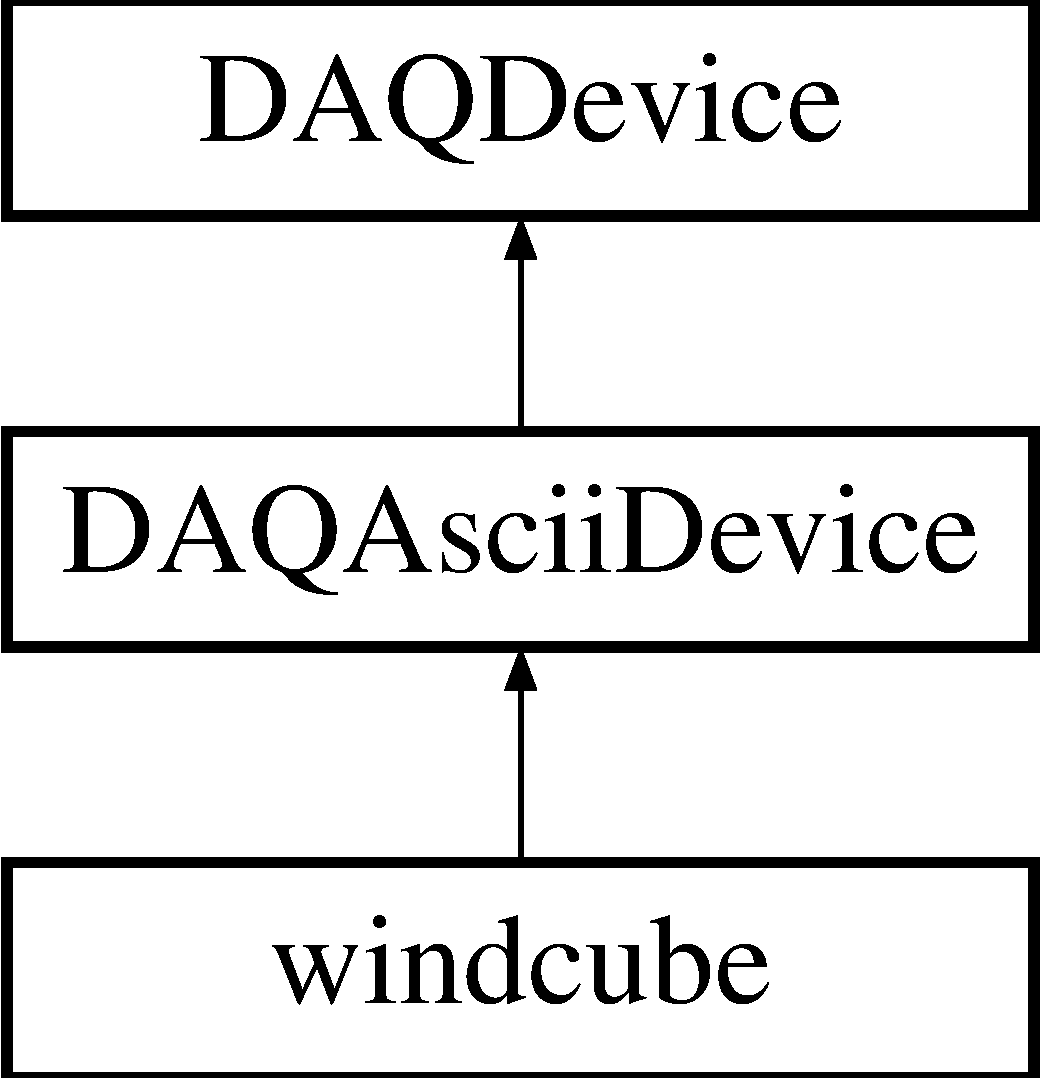
\includegraphics[height=3.000000cm]{classwindcube}
\end{center}
\end{figure}
\subsection*{Public Member Functions}
\begin{DoxyCompactItemize}
\item 
\hyperlink{classwindcube_a8ae21721598a79437be9852ccaa266aa}{windcube} ()
\item 
\hyperlink{classwindcube_a08dd08e8a45cd9082be7bd488a8d230f}{$\sim$windcube} ()
\item 
void \hyperlink{classwindcube_ab15ca79d204a336abbd7ab5245ec9e55}{set\-Config\-Defaults} ()
\item 
int \hyperlink{classwindcube_a369ea13a1dcd471ad51250f89151364b}{read\-Header} (const char $\ast$\hyperlink{classDAQDevice_a7f9cda7cf5b41f6b134c313477e9644b}{filename})
\item 
unsigned int \hyperlink{classwindcube_a705808162810f8f4430e2bc3ca04a181}{get\-Sensor\-Group} ()
\item 
void \hyperlink{classwindcube_ab0a74d15ddda343b34ff4b28389fa811}{read\-Data} (std\-::string full\-\_\-filename)
\item 
int \hyperlink{classwindcube_a72691b4435de39d059542a1ccd064683}{parse\-Data} (char $\ast$\hyperlink{classDAQDevice_ab661aa5c5b4bafe78354f5169b1c7d2f}{buffer}, struct timeval $\ast$l\-\_\-t\-Data, double $\ast$sensor\-\_\-values)
\end{DoxyCompactItemize}
\subsection*{Private Attributes}
\begin{DoxyCompactItemize}
\item 
double \hyperlink{classwindcube_ada525fe40090dafeb8d7dae911ed9ac4}{elevation\-\_\-angle}
\item 
double $\ast$ \hyperlink{classwindcube_a6080ff141d176b3bb7e0dbc655ed46e9}{altitudes}
\item 
int \hyperlink{classwindcube_a283219a5fa65543bef16fdb3c8598260}{initial\-\_\-position}
\item 
struct timeval \hyperlink{classwindcube_aecb46d84c92acb6390ef5d33ba33957c}{initial\-\_\-timestamp}
\item 
double \hyperlink{classwindcube_a7c023ee8ccc3900b6544136f1e845e3f}{gain}
\end{DoxyCompactItemize}
\subsection*{Additional Inherited Members}


\subsection{Constructor \& Destructor Documentation}
\hypertarget{classwindcube_a8ae21721598a79437be9852ccaa266aa}{\index{windcube@{windcube}!windcube@{windcube}}
\index{windcube@{windcube}!windcube@{windcube}}
\subsubsection[{windcube}]{\setlength{\rightskip}{0pt plus 5cm}windcube\-::windcube (
\begin{DoxyParamCaption}
{}
\end{DoxyParamCaption}
)}}\label{classwindcube_a8ae21721598a79437be9852ccaa266aa}
\hypertarget{classwindcube_a08dd08e8a45cd9082be7bd488a8d230f}{\index{windcube@{windcube}!$\sim$windcube@{$\sim$windcube}}
\index{$\sim$windcube@{$\sim$windcube}!windcube@{windcube}}
\subsubsection[{$\sim$windcube}]{\setlength{\rightskip}{0pt plus 5cm}windcube\-::$\sim$windcube (
\begin{DoxyParamCaption}
{}
\end{DoxyParamCaption}
)}}\label{classwindcube_a08dd08e8a45cd9082be7bd488a8d230f}


\subsection{Member Function Documentation}
\hypertarget{classwindcube_a705808162810f8f4430e2bc3ca04a181}{\index{windcube@{windcube}!get\-Sensor\-Group@{get\-Sensor\-Group}}
\index{get\-Sensor\-Group@{get\-Sensor\-Group}!windcube@{windcube}}
\subsubsection[{get\-Sensor\-Group}]{\setlength{\rightskip}{0pt plus 5cm}unsigned int windcube\-::get\-Sensor\-Group (
\begin{DoxyParamCaption}
{}
\end{DoxyParamCaption}
)\hspace{0.3cm}{\ttfamily [virtual]}}}\label{classwindcube_a705808162810f8f4430e2bc3ca04a181}
Define a sensor group number for all the availble sensor group files 

Reimplemented from \hyperlink{classDAQDevice_a61d08492a11c30944dfaf3b86115abe8}{D\-A\-Q\-Device}.

\hypertarget{classwindcube_a72691b4435de39d059542a1ccd064683}{\index{windcube@{windcube}!parse\-Data@{parse\-Data}}
\index{parse\-Data@{parse\-Data}!windcube@{windcube}}
\subsubsection[{parse\-Data}]{\setlength{\rightskip}{0pt plus 5cm}int windcube\-::parse\-Data (
\begin{DoxyParamCaption}
\item[{char $\ast$}]{line, }
\item[{struct timeval $\ast$}]{l\-\_\-t\-Data, }
\item[{double $\ast$}]{sensor\-Value}
\end{DoxyParamCaption}
)\hspace{0.3cm}{\ttfamily [virtual]}}}\label{classwindcube_a72691b4435de39d059542a1ccd064683}
Read the data from the current line of the data file. \begin{DoxyReturn}{Returns}
-\/1 no data found, skip storage 0 sucess, store data, 1 read another line 
\end{DoxyReturn}


Reimplemented from \hyperlink{classDAQAsciiDevice_a9c20d9d69af4ba1641dbc82dd5be2aa5}{D\-A\-Q\-Ascii\-Device}.

\hypertarget{classwindcube_ab0a74d15ddda343b34ff4b28389fa811}{\index{windcube@{windcube}!read\-Data@{read\-Data}}
\index{read\-Data@{read\-Data}!windcube@{windcube}}
\subsubsection[{read\-Data}]{\setlength{\rightskip}{0pt plus 5cm}void windcube\-::read\-Data (
\begin{DoxyParamCaption}
\item[{std\-::string}]{full\-\_\-filename}
\end{DoxyParamCaption}
)\hspace{0.3cm}{\ttfamily [virtual]}}}\label{classwindcube_ab0a74d15ddda343b34ff4b28389fa811}


Reimplemented from \hyperlink{classDAQAsciiDevice_a0d9b17803680d966c7025ca6f174cef0}{D\-A\-Q\-Ascii\-Device}.

\hypertarget{classwindcube_a369ea13a1dcd471ad51250f89151364b}{\index{windcube@{windcube}!read\-Header@{read\-Header}}
\index{read\-Header@{read\-Header}!windcube@{windcube}}
\subsubsection[{read\-Header}]{\setlength{\rightskip}{0pt plus 5cm}int windcube\-::read\-Header (
\begin{DoxyParamCaption}
\item[{const char $\ast$}]{header}
\end{DoxyParamCaption}
)\hspace{0.3cm}{\ttfamily [virtual]}}}\label{classwindcube_a369ea13a1dcd471ad51250f89151364b}
Get time until next sample and it's id 

Reimplemented from \hyperlink{classDAQAsciiDevice_a5fce725c52b70ef2f56a34b32a03e15d}{D\-A\-Q\-Ascii\-Device}.

\hypertarget{classwindcube_ab15ca79d204a336abbd7ab5245ec9e55}{\index{windcube@{windcube}!set\-Config\-Defaults@{set\-Config\-Defaults}}
\index{set\-Config\-Defaults@{set\-Config\-Defaults}!windcube@{windcube}}
\subsubsection[{set\-Config\-Defaults}]{\setlength{\rightskip}{0pt plus 5cm}void windcube\-::set\-Config\-Defaults (
\begin{DoxyParamCaption}
{}
\end{DoxyParamCaption}
)\hspace{0.3cm}{\ttfamily [virtual]}}}\label{classwindcube_ab15ca79d204a336abbd7ab5245ec9e55}
The function is called before reading the configuration from the inifile. Use this fucntion in the module specific implementation to override the standard defaults 

Reimplemented from \hyperlink{classDAQDevice_a7685cec80865752cc0ef3ab49c6c2277}{D\-A\-Q\-Device}.



\subsection{Member Data Documentation}
\hypertarget{classwindcube_a6080ff141d176b3bb7e0dbc655ed46e9}{\index{windcube@{windcube}!altitudes@{altitudes}}
\index{altitudes@{altitudes}!windcube@{windcube}}
\subsubsection[{altitudes}]{\setlength{\rightskip}{0pt plus 5cm}double$\ast$ windcube\-::altitudes\hspace{0.3cm}{\ttfamily [private]}}}\label{classwindcube_a6080ff141d176b3bb7e0dbc655ed46e9}
\hypertarget{classwindcube_ada525fe40090dafeb8d7dae911ed9ac4}{\index{windcube@{windcube}!elevation\-\_\-angle@{elevation\-\_\-angle}}
\index{elevation\-\_\-angle@{elevation\-\_\-angle}!windcube@{windcube}}
\subsubsection[{elevation\-\_\-angle}]{\setlength{\rightskip}{0pt plus 5cm}double windcube\-::elevation\-\_\-angle\hspace{0.3cm}{\ttfamily [private]}}}\label{classwindcube_ada525fe40090dafeb8d7dae911ed9ac4}
\hypertarget{classwindcube_a7c023ee8ccc3900b6544136f1e845e3f}{\index{windcube@{windcube}!gain@{gain}}
\index{gain@{gain}!windcube@{windcube}}
\subsubsection[{gain}]{\setlength{\rightskip}{0pt plus 5cm}double windcube\-::gain\hspace{0.3cm}{\ttfamily [private]}}}\label{classwindcube_a7c023ee8ccc3900b6544136f1e845e3f}
\hypertarget{classwindcube_a283219a5fa65543bef16fdb3c8598260}{\index{windcube@{windcube}!initial\-\_\-position@{initial\-\_\-position}}
\index{initial\-\_\-position@{initial\-\_\-position}!windcube@{windcube}}
\subsubsection[{initial\-\_\-position}]{\setlength{\rightskip}{0pt plus 5cm}int windcube\-::initial\-\_\-position\hspace{0.3cm}{\ttfamily [private]}}}\label{classwindcube_a283219a5fa65543bef16fdb3c8598260}
\hypertarget{classwindcube_aecb46d84c92acb6390ef5d33ba33957c}{\index{windcube@{windcube}!initial\-\_\-timestamp@{initial\-\_\-timestamp}}
\index{initial\-\_\-timestamp@{initial\-\_\-timestamp}!windcube@{windcube}}
\subsubsection[{initial\-\_\-timestamp}]{\setlength{\rightskip}{0pt plus 5cm}struct timeval windcube\-::initial\-\_\-timestamp\hspace{0.3cm}{\ttfamily [private]}}}\label{classwindcube_aecb46d84c92acb6390ef5d33ba33957c}


The documentation for this class was generated from the following files\-:\begin{DoxyCompactItemize}
\item 
/home/ntj/\-Development/phd/kitcube-\/tools/src/kitcube-\/devices/\hyperlink{windcube_8h}{windcube.\-h}\item 
/home/ntj/\-Development/phd/kitcube-\/tools/src/kitcube-\/devices/\hyperlink{windcube_8cpp}{windcube.\-cpp}\end{DoxyCompactItemize}

\hypertarget{classwindtracer}{\section{windtracer Class Reference}
\label{classwindtracer}\index{windtracer@{windtracer}}
}


{\ttfamily \#include $<$windtracer.\-h$>$}

Inheritance diagram for windtracer\-:\begin{figure}[H]
\begin{center}
\leavevmode
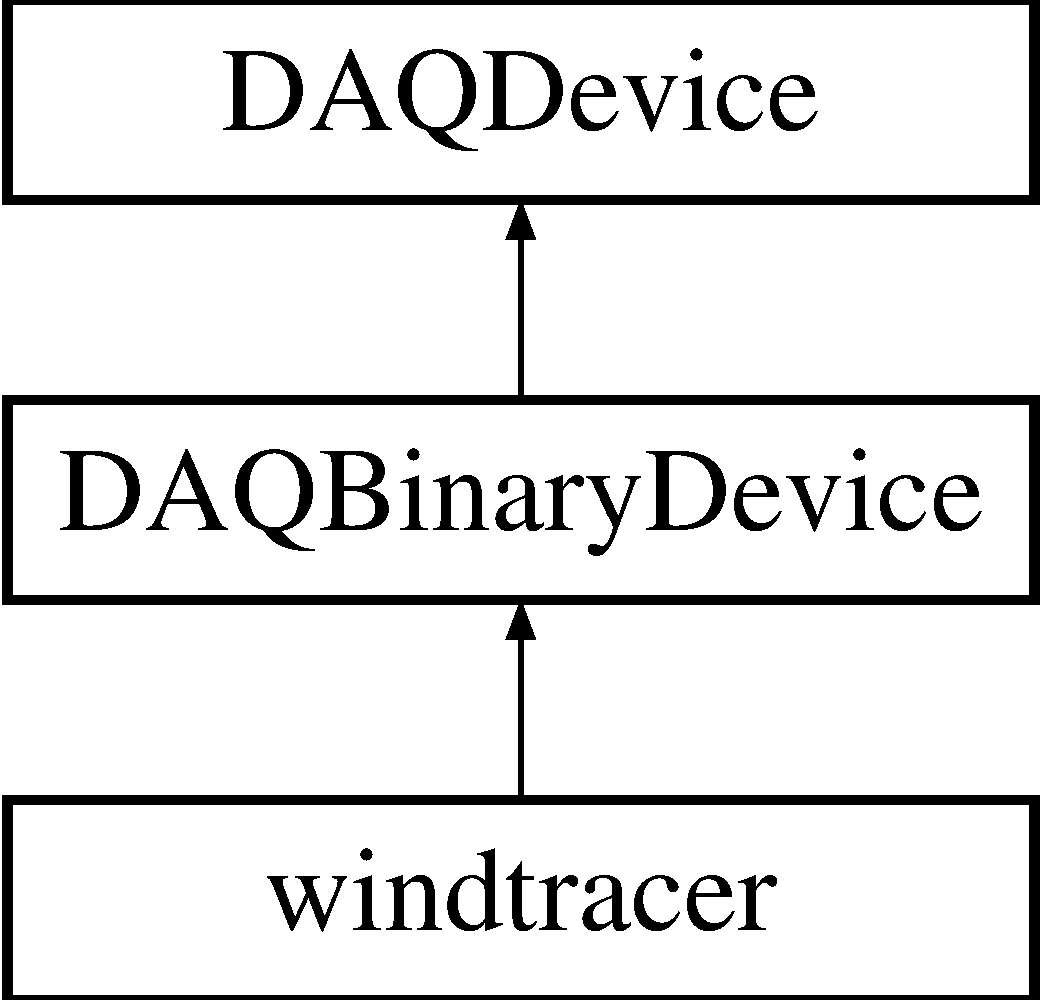
\includegraphics[height=3.000000cm]{classwindtracer}
\end{center}
\end{figure}
\subsection*{Public Member Functions}
\begin{DoxyCompactItemize}
\item 
\hyperlink{classwindtracer_a3f39c3cdfe087c887a78a85f7a5bed36}{windtracer} ()
\item 
\hyperlink{classwindtracer_abfca68f0babb9454b1bc6776d8b3940e}{$\sim$windtracer} ()
\item 
void \hyperlink{classwindtracer_a6e14dbde1b75db6e2c995b86964316ea}{set\-Config\-Defaults} ()
\item 
unsigned int \hyperlink{classwindtracer_a55ce8f421fa720fa2f6976feb229f255}{get\-Sensor\-Group} ()
\item 
int \hyperlink{classwindtracer_ae85ea00fe9c7849b4b29e2efe644383c}{read\-Header} (const char $\ast$header)
\item 
void \hyperlink{classwindtracer_a3017c180cdd51ab93c5b73c2f84059f5}{read\-Data} (std\-::string full\-\_\-filename)
\item 
void \hyperlink{classwindtracer_a586683ce39f917f833eb2d1478c5a108}{parse\-Data} (u\-\_\-char $\ast$\hyperlink{classDAQDevice_ab661aa5c5b4bafe78354f5169b1c7d2f}{buffer}, struct \hyperlink{structRecordHeader}{Record\-Header} $\ast$record\-\_\-header, struct \hyperlink{structScanInfo}{Scan\-Info} $\ast$$\ast$scan\-\_\-info, struct \hyperlink{structProductPulseInfo}{Product\-Pulse\-Info} $\ast$$\ast$pulse\-\_\-info, float $\ast$$\ast$sensor\-\_\-values, u\-\_\-int32\-\_\-t $\ast$sensor\-\_\-values\-\_\-length)
\item 
int \hyperlink{classwindtracer_a4921e9eaa0f568b3119bd8f253484388}{create\-\_\-data\-\_\-table} ()
\item 
const char $\ast$ \hyperlink{classwindtracer_abb6a7e64e508dec0f0e10cf8af76fc9c}{get\-Data\-Dir} ()
\end{DoxyCompactItemize}
\subsection*{Private Member Functions}
\begin{DoxyCompactItemize}
\item 
int \hyperlink{classwindtracer_af9d739964c034029c99e283a283b506f}{create\-\_\-data\-\_\-table\-\_\-name} (std\-::string \&data\-\_\-table\-\_\-name)
\end{DoxyCompactItemize}
\subsection*{Private Attributes}
\begin{DoxyCompactItemize}
\item 
unsigned char $\ast$ \hyperlink{classwindtracer_a0fd43967f940c29d8977eb1240696d81}{header\-Raw}
\item 
std\-::string \hyperlink{classwindtracer_aa0b5d56c9d831360a9a57b6652a9bce0}{experiment\-Name}
\item 
unsigned int \hyperlink{classwindtracer_ac1445c6c8d23eb15c58034163ca8aacd}{t\-Sample}
\item 
struct timeval \hyperlink{classwindtracer_ac5ff90382dacf3ee0a23602f7416b3b5}{t\-Ref}
\item 
struct \hyperlink{structConfigurationRecord}{Configuration\-Record} \hyperlink{classwindtracer_a5d67866d830f38f37ac8b0c69c6f7378}{config\-\_\-record}
\item 
u\-\_\-int32\-\_\-t \hyperlink{classwindtracer_ade65f374d3b610d90658a3d0bbbf5111}{config\-\_\-text\-\_\-block\-\_\-length}
\item 
int \hyperlink{classwindtracer_a6352be627e3d05ee0767550ede2654b6}{range\-\_\-gates}
\item 
double $\ast$ \hyperlink{classwindtracer_af81c7fd1af56fc55b07d4c2253a409d1}{range\-\_\-gate\-\_\-center}
\item 
double $\ast$ \hyperlink{classwindtracer_af1c976835951ac79c4f26219fe1eac20}{range\-\_\-gate\-\_\-start}
\item 
double $\ast$ \hyperlink{classwindtracer_a61691581de3e6322086ba201d2c468a2}{range\-\_\-gate\-\_\-end}
\item 
int \hyperlink{classwindtracer_ac203ed51cd1cee3e910adcc6ad007bb0}{num\-\_\-sensors}
\item 
int \hyperlink{classwindtracer_a7f9c0a2573aa664a8b7a7ba046ae2757}{num\-\_\-aux\-\_\-sensors}
\end{DoxyCompactItemize}
\subsection*{Additional Inherited Members}


\subsection{Constructor \& Destructor Documentation}
\hypertarget{classwindtracer_a3f39c3cdfe087c887a78a85f7a5bed36}{\index{windtracer@{windtracer}!windtracer@{windtracer}}
\index{windtracer@{windtracer}!windtracer@{windtracer}}
\subsubsection[{windtracer}]{\setlength{\rightskip}{0pt plus 5cm}windtracer\-::windtracer (
\begin{DoxyParamCaption}
{}
\end{DoxyParamCaption}
)}}\label{classwindtracer_a3f39c3cdfe087c887a78a85f7a5bed36}
\hypertarget{classwindtracer_abfca68f0babb9454b1bc6776d8b3940e}{\index{windtracer@{windtracer}!$\sim$windtracer@{$\sim$windtracer}}
\index{$\sim$windtracer@{$\sim$windtracer}!windtracer@{windtracer}}
\subsubsection[{$\sim$windtracer}]{\setlength{\rightskip}{0pt plus 5cm}windtracer\-::$\sim$windtracer (
\begin{DoxyParamCaption}
{}
\end{DoxyParamCaption}
)}}\label{classwindtracer_abfca68f0babb9454b1bc6776d8b3940e}


\subsection{Member Function Documentation}
\hypertarget{classwindtracer_a4921e9eaa0f568b3119bd8f253484388}{\index{windtracer@{windtracer}!create\-\_\-data\-\_\-table@{create\-\_\-data\-\_\-table}}
\index{create\-\_\-data\-\_\-table@{create\-\_\-data\-\_\-table}!windtracer@{windtracer}}
\subsubsection[{create\-\_\-data\-\_\-table}]{\setlength{\rightskip}{0pt plus 5cm}int windtracer\-::create\-\_\-data\-\_\-table (
\begin{DoxyParamCaption}
{}
\end{DoxyParamCaption}
)\hspace{0.3cm}{\ttfamily [virtual]}}}\label{classwindtracer_a4921e9eaa0f568b3119bd8f253484388}
Create data table, if it doesn't exist. The function is called by \hyperlink{classDAQDevice_a32f118d291f1c7b8fe47a16474b825e2}{open\-Database()}. 

Reimplemented from \hyperlink{classDAQDevice_ac4867b7e5aff2d5c404d6eb1053dda71}{D\-A\-Q\-Device}.

\hypertarget{classwindtracer_af9d739964c034029c99e283a283b506f}{\index{windtracer@{windtracer}!create\-\_\-data\-\_\-table\-\_\-name@{create\-\_\-data\-\_\-table\-\_\-name}}
\index{create\-\_\-data\-\_\-table\-\_\-name@{create\-\_\-data\-\_\-table\-\_\-name}!windtracer@{windtracer}}
\subsubsection[{create\-\_\-data\-\_\-table\-\_\-name}]{\setlength{\rightskip}{0pt plus 5cm}int windtracer\-::create\-\_\-data\-\_\-table\-\_\-name (
\begin{DoxyParamCaption}
\item[{std\-::string \&}]{data\-\_\-table\-\_\-name}
\end{DoxyParamCaption}
)\hspace{0.3cm}{\ttfamily [private]}, {\ttfamily [virtual]}}}\label{classwindtracer_af9d739964c034029c99e283a283b506f}


Reimplemented from \hyperlink{classDAQDevice_add621117663b1aa2b3c3efcc115a8126}{D\-A\-Q\-Device}.

\hypertarget{classwindtracer_abb6a7e64e508dec0f0e10cf8af76fc9c}{\index{windtracer@{windtracer}!get\-Data\-Dir@{get\-Data\-Dir}}
\index{get\-Data\-Dir@{get\-Data\-Dir}!windtracer@{windtracer}}
\subsubsection[{get\-Data\-Dir}]{\setlength{\rightskip}{0pt plus 5cm}const char $\ast$ windtracer\-::get\-Data\-Dir (
\begin{DoxyParamCaption}
{}
\end{DoxyParamCaption}
)\hspace{0.3cm}{\ttfamily [virtual]}}}\label{classwindtracer_abb6a7e64e508dec0f0e10cf8af76fc9c}


Reimplemented from \hyperlink{classDAQDevice_a7d7d41f0c1496221e589d84b38d1c865}{D\-A\-Q\-Device}.

\hypertarget{classwindtracer_a55ce8f421fa720fa2f6976feb229f255}{\index{windtracer@{windtracer}!get\-Sensor\-Group@{get\-Sensor\-Group}}
\index{get\-Sensor\-Group@{get\-Sensor\-Group}!windtracer@{windtracer}}
\subsubsection[{get\-Sensor\-Group}]{\setlength{\rightskip}{0pt plus 5cm}unsigned int windtracer\-::get\-Sensor\-Group (
\begin{DoxyParamCaption}
{}
\end{DoxyParamCaption}
)\hspace{0.3cm}{\ttfamily [virtual]}}}\label{classwindtracer_a55ce8f421fa720fa2f6976feb229f255}
Return the number of the sensor group 

Reimplemented from \hyperlink{classDAQDevice_a61d08492a11c30944dfaf3b86115abe8}{D\-A\-Q\-Device}.

\hypertarget{classwindtracer_a586683ce39f917f833eb2d1478c5a108}{\index{windtracer@{windtracer}!parse\-Data@{parse\-Data}}
\index{parse\-Data@{parse\-Data}!windtracer@{windtracer}}
\subsubsection[{parse\-Data}]{\setlength{\rightskip}{0pt plus 5cm}void windtracer\-::parse\-Data (
\begin{DoxyParamCaption}
\item[{u\-\_\-char $\ast$}]{buffer, }
\item[{struct {\bf Record\-Header} $\ast$}]{record\-\_\-header, }
\item[{struct {\bf Scan\-Info} $\ast$$\ast$}]{scan\-\_\-info, }
\item[{struct {\bf Product\-Pulse\-Info} $\ast$$\ast$}]{pulse\-\_\-info, }
\item[{float $\ast$$\ast$}]{sensor\-\_\-values, }
\item[{u\-\_\-int32\-\_\-t $\ast$}]{sensor\-\_\-values\-\_\-length}
\end{DoxyParamCaption}
)}}\label{classwindtracer_a586683ce39f917f833eb2d1478c5a108}
\hypertarget{classwindtracer_a3017c180cdd51ab93c5b73c2f84059f5}{\index{windtracer@{windtracer}!read\-Data@{read\-Data}}
\index{read\-Data@{read\-Data}!windtracer@{windtracer}}
\subsubsection[{read\-Data}]{\setlength{\rightskip}{0pt plus 5cm}void windtracer\-::read\-Data (
\begin{DoxyParamCaption}
\item[{std\-::string}]{full\-\_\-filename}
\end{DoxyParamCaption}
)\hspace{0.3cm}{\ttfamily [virtual]}}}\label{classwindtracer_a3017c180cdd51ab93c5b73c2f84059f5}


Reimplemented from \hyperlink{classDAQBinaryDevice_a725281822b7945b8c1154d079c0011ff}{D\-A\-Q\-Binary\-Device}.

\hypertarget{classwindtracer_ae85ea00fe9c7849b4b29e2efe644383c}{\index{windtracer@{windtracer}!read\-Header@{read\-Header}}
\index{read\-Header@{read\-Header}!windtracer@{windtracer}}
\subsubsection[{read\-Header}]{\setlength{\rightskip}{0pt plus 5cm}int windtracer\-::read\-Header (
\begin{DoxyParamCaption}
\item[{const char $\ast$}]{header}
\end{DoxyParamCaption}
)\hspace{0.3cm}{\ttfamily [virtual]}}}\label{classwindtracer_ae85ea00fe9c7849b4b29e2efe644383c}
Get time until next sample and it's id 

Reimplemented from \hyperlink{classDAQDevice_af5fa373af9a089c18c7fd1d662db144f}{D\-A\-Q\-Device}.

\hypertarget{classwindtracer_a6e14dbde1b75db6e2c995b86964316ea}{\index{windtracer@{windtracer}!set\-Config\-Defaults@{set\-Config\-Defaults}}
\index{set\-Config\-Defaults@{set\-Config\-Defaults}!windtracer@{windtracer}}
\subsubsection[{set\-Config\-Defaults}]{\setlength{\rightskip}{0pt plus 5cm}void windtracer\-::set\-Config\-Defaults (
\begin{DoxyParamCaption}
{}
\end{DoxyParamCaption}
)\hspace{0.3cm}{\ttfamily [virtual]}}}\label{classwindtracer_a6e14dbde1b75db6e2c995b86964316ea}
The function is called before reading the configuration from the inifile. Use this fucntion in the module specific implementation to override the standard defaults 

Reimplemented from \hyperlink{classDAQDevice_a7685cec80865752cc0ef3ab49c6c2277}{D\-A\-Q\-Device}.



\subsection{Member Data Documentation}
\hypertarget{classwindtracer_a5d67866d830f38f37ac8b0c69c6f7378}{\index{windtracer@{windtracer}!config\-\_\-record@{config\-\_\-record}}
\index{config\-\_\-record@{config\-\_\-record}!windtracer@{windtracer}}
\subsubsection[{config\-\_\-record}]{\setlength{\rightskip}{0pt plus 5cm}struct {\bf Configuration\-Record} windtracer\-::config\-\_\-record\hspace{0.3cm}{\ttfamily [private]}}}\label{classwindtracer_a5d67866d830f38f37ac8b0c69c6f7378}
\hypertarget{classwindtracer_ade65f374d3b610d90658a3d0bbbf5111}{\index{windtracer@{windtracer}!config\-\_\-text\-\_\-block\-\_\-length@{config\-\_\-text\-\_\-block\-\_\-length}}
\index{config\-\_\-text\-\_\-block\-\_\-length@{config\-\_\-text\-\_\-block\-\_\-length}!windtracer@{windtracer}}
\subsubsection[{config\-\_\-text\-\_\-block\-\_\-length}]{\setlength{\rightskip}{0pt plus 5cm}u\-\_\-int32\-\_\-t windtracer\-::config\-\_\-text\-\_\-block\-\_\-length\hspace{0.3cm}{\ttfamily [private]}}}\label{classwindtracer_ade65f374d3b610d90658a3d0bbbf5111}
\hypertarget{classwindtracer_aa0b5d56c9d831360a9a57b6652a9bce0}{\index{windtracer@{windtracer}!experiment\-Name@{experiment\-Name}}
\index{experiment\-Name@{experiment\-Name}!windtracer@{windtracer}}
\subsubsection[{experiment\-Name}]{\setlength{\rightskip}{0pt plus 5cm}std\-::string windtracer\-::experiment\-Name\hspace{0.3cm}{\ttfamily [private]}}}\label{classwindtracer_aa0b5d56c9d831360a9a57b6652a9bce0}
\hypertarget{classwindtracer_a0fd43967f940c29d8977eb1240696d81}{\index{windtracer@{windtracer}!header\-Raw@{header\-Raw}}
\index{header\-Raw@{header\-Raw}!windtracer@{windtracer}}
\subsubsection[{header\-Raw}]{\setlength{\rightskip}{0pt plus 5cm}unsigned char$\ast$ windtracer\-::header\-Raw\hspace{0.3cm}{\ttfamily [private]}}}\label{classwindtracer_a0fd43967f940c29d8977eb1240696d81}
\hypertarget{classwindtracer_a7f9c0a2573aa664a8b7a7ba046ae2757}{\index{windtracer@{windtracer}!num\-\_\-aux\-\_\-sensors@{num\-\_\-aux\-\_\-sensors}}
\index{num\-\_\-aux\-\_\-sensors@{num\-\_\-aux\-\_\-sensors}!windtracer@{windtracer}}
\subsubsection[{num\-\_\-aux\-\_\-sensors}]{\setlength{\rightskip}{0pt plus 5cm}int windtracer\-::num\-\_\-aux\-\_\-sensors\hspace{0.3cm}{\ttfamily [private]}}}\label{classwindtracer_a7f9c0a2573aa664a8b7a7ba046ae2757}
\hypertarget{classwindtracer_ac203ed51cd1cee3e910adcc6ad007bb0}{\index{windtracer@{windtracer}!num\-\_\-sensors@{num\-\_\-sensors}}
\index{num\-\_\-sensors@{num\-\_\-sensors}!windtracer@{windtracer}}
\subsubsection[{num\-\_\-sensors}]{\setlength{\rightskip}{0pt plus 5cm}int windtracer\-::num\-\_\-sensors\hspace{0.3cm}{\ttfamily [private]}}}\label{classwindtracer_ac203ed51cd1cee3e910adcc6ad007bb0}
\hypertarget{classwindtracer_af81c7fd1af56fc55b07d4c2253a409d1}{\index{windtracer@{windtracer}!range\-\_\-gate\-\_\-center@{range\-\_\-gate\-\_\-center}}
\index{range\-\_\-gate\-\_\-center@{range\-\_\-gate\-\_\-center}!windtracer@{windtracer}}
\subsubsection[{range\-\_\-gate\-\_\-center}]{\setlength{\rightskip}{0pt plus 5cm}double$\ast$ windtracer\-::range\-\_\-gate\-\_\-center\hspace{0.3cm}{\ttfamily [private]}}}\label{classwindtracer_af81c7fd1af56fc55b07d4c2253a409d1}
\hypertarget{classwindtracer_a61691581de3e6322086ba201d2c468a2}{\index{windtracer@{windtracer}!range\-\_\-gate\-\_\-end@{range\-\_\-gate\-\_\-end}}
\index{range\-\_\-gate\-\_\-end@{range\-\_\-gate\-\_\-end}!windtracer@{windtracer}}
\subsubsection[{range\-\_\-gate\-\_\-end}]{\setlength{\rightskip}{0pt plus 5cm}double $\ast$ windtracer\-::range\-\_\-gate\-\_\-end\hspace{0.3cm}{\ttfamily [private]}}}\label{classwindtracer_a61691581de3e6322086ba201d2c468a2}
\hypertarget{classwindtracer_af1c976835951ac79c4f26219fe1eac20}{\index{windtracer@{windtracer}!range\-\_\-gate\-\_\-start@{range\-\_\-gate\-\_\-start}}
\index{range\-\_\-gate\-\_\-start@{range\-\_\-gate\-\_\-start}!windtracer@{windtracer}}
\subsubsection[{range\-\_\-gate\-\_\-start}]{\setlength{\rightskip}{0pt plus 5cm}double $\ast$ windtracer\-::range\-\_\-gate\-\_\-start\hspace{0.3cm}{\ttfamily [private]}}}\label{classwindtracer_af1c976835951ac79c4f26219fe1eac20}
\hypertarget{classwindtracer_a6352be627e3d05ee0767550ede2654b6}{\index{windtracer@{windtracer}!range\-\_\-gates@{range\-\_\-gates}}
\index{range\-\_\-gates@{range\-\_\-gates}!windtracer@{windtracer}}
\subsubsection[{range\-\_\-gates}]{\setlength{\rightskip}{0pt plus 5cm}int windtracer\-::range\-\_\-gates\hspace{0.3cm}{\ttfamily [private]}}}\label{classwindtracer_a6352be627e3d05ee0767550ede2654b6}
\hypertarget{classwindtracer_ac5ff90382dacf3ee0a23602f7416b3b5}{\index{windtracer@{windtracer}!t\-Ref@{t\-Ref}}
\index{t\-Ref@{t\-Ref}!windtracer@{windtracer}}
\subsubsection[{t\-Ref}]{\setlength{\rightskip}{0pt plus 5cm}struct timeval windtracer\-::t\-Ref\hspace{0.3cm}{\ttfamily [private]}}}\label{classwindtracer_ac5ff90382dacf3ee0a23602f7416b3b5}
\hypertarget{classwindtracer_ac1445c6c8d23eb15c58034163ca8aacd}{\index{windtracer@{windtracer}!t\-Sample@{t\-Sample}}
\index{t\-Sample@{t\-Sample}!windtracer@{windtracer}}
\subsubsection[{t\-Sample}]{\setlength{\rightskip}{0pt plus 5cm}unsigned int windtracer\-::t\-Sample\hspace{0.3cm}{\ttfamily [private]}}}\label{classwindtracer_ac1445c6c8d23eb15c58034163ca8aacd}


The documentation for this class was generated from the following files\-:\begin{DoxyCompactItemize}
\item 
/home/ntj/\-Development/phd/kitcube-\/tools/src/kitcube-\/devices/\hyperlink{windtracer_8h}{windtracer.\-h}\item 
/home/ntj/\-Development/phd/kitcube-\/tools/src/kitcube-\/devices/\hyperlink{windtracer_8cpp}{windtracer.\-cpp}\end{DoxyCompactItemize}

\hypertarget{classwolkenkamera}{\section{wolkenkamera Class Reference}
\label{classwolkenkamera}\index{wolkenkamera@{wolkenkamera}}
}


{\ttfamily \#include $<$wolkenkamera.\-h$>$}

Inheritance diagram for wolkenkamera\-:\begin{figure}[H]
\begin{center}
\leavevmode
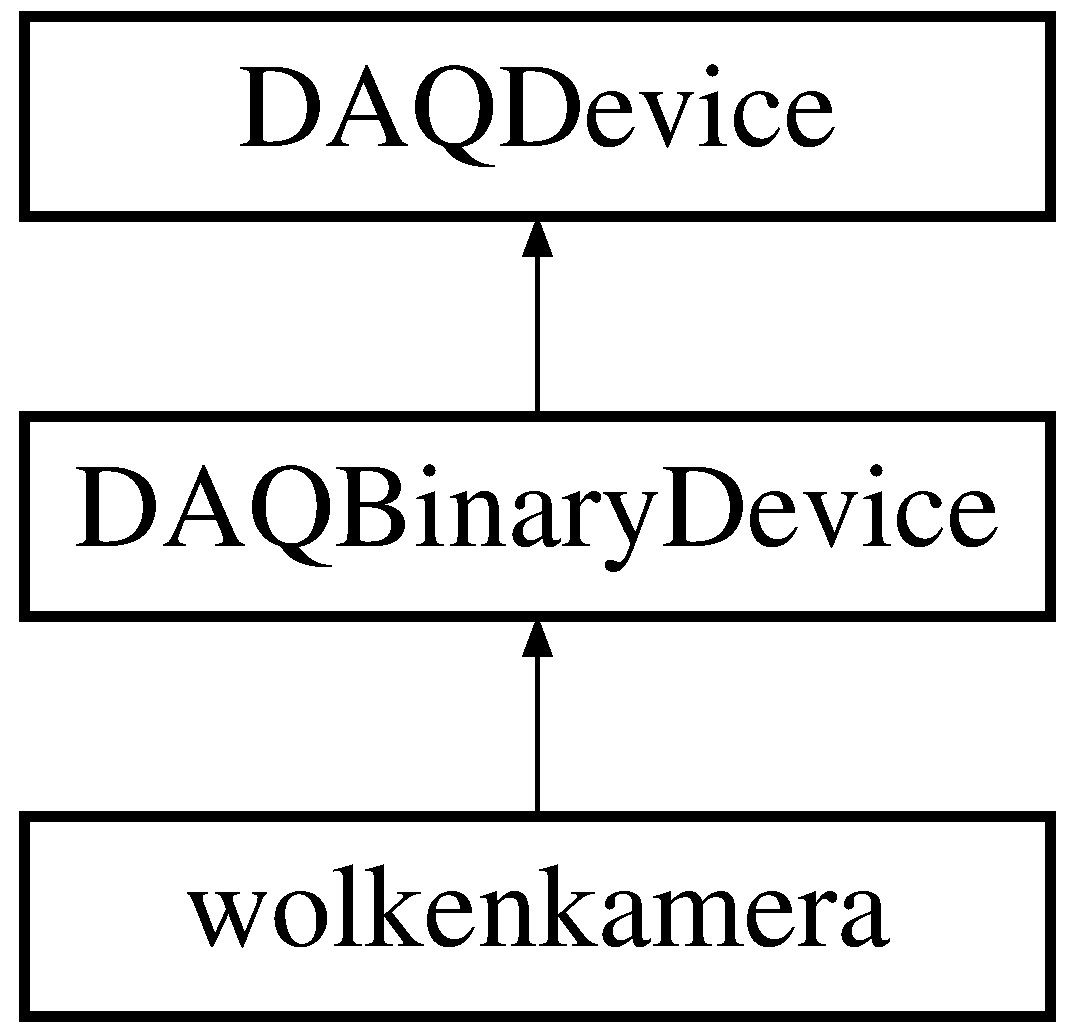
\includegraphics[height=3.000000cm]{classwolkenkamera}
\end{center}
\end{figure}
\subsection*{Public Member Functions}
\begin{DoxyCompactItemize}
\item 
\hyperlink{classwolkenkamera_ae13f001a967338d8301ece76e9046980}{wolkenkamera} ()
\item 
\hyperlink{classwolkenkamera_a1f773650109aff935dcf89246c51da93}{$\sim$wolkenkamera} ()
\item 
void \hyperlink{classwolkenkamera_a718522b6c0780be9819af11b9e6a81dd}{set\-Config\-Defaults} ()
\item 
const char $\ast$ \hyperlink{classwolkenkamera_ac4f55fd3e4b97532af5774daab350358}{get\-Data\-Dir} ()
\item 
unsigned int \hyperlink{classwolkenkamera_abf6bb4f8fe052838bb2cf1905ce15caa}{get\-Sensor\-Group} ()
\item 
int \hyperlink{classwolkenkamera_acbca7eeed93a4686d5661c997c24ac7b}{read\-Header} (const char $\ast$header)
\item 
void \hyperlink{classwolkenkamera_ab5b110a1434326c6f843390fc91c6f1b}{write\-Header} ()
\item 
void \hyperlink{classwolkenkamera_a9d63655c35a98dec0583b27a67b292ce}{read\-Data} (std\-::string full\-\_\-filename)
\item 
void \hyperlink{classwolkenkamera_ab6cb0bfc7780ca531c10d18ff7b7ab13}{update\-Data\-Set} (unsigned char $\ast$buf)
\item 
long \hyperlink{classwolkenkamera_aada77e474f3ed7097178c17e03c78b5b}{get\-File\-Number} (char $\ast$\hyperlink{classDAQDevice_a7f9cda7cf5b41f6b134c313477e9644b}{filename})
\end{DoxyCompactItemize}
\subsection*{Private Attributes}
\begin{DoxyCompactItemize}
\item 
unsigned char $\ast$ \hyperlink{classwolkenkamera_a30e481479bddffe39a354b51ef4c7b67}{header\-Raw}
\item 
std\-::string \hyperlink{classwolkenkamera_aa91268dbd611187b783c89ef62dbcfd5}{experiment\-Name}
\item 
unsigned long \hyperlink{classwolkenkamera_a5f45de1bc4646afdc2fd112a724e48bd}{t\-Sample}
\item 
struct timeval \hyperlink{classwolkenkamera_afff90fa33b0ee850413fee6e2aa4563f}{t\-Ref}
\end{DoxyCompactItemize}
\subsection*{Additional Inherited Members}


\subsection{Detailed Description}
Implementation for the ceilometer D\-A\-Q device.

\begin{DoxyRefDesc}{Todo}
\item[\hyperlink{todo__todo000018}{Todo}]Move return string to the argument list\end{DoxyRefDesc}


\subsection{Constructor \& Destructor Documentation}
\hypertarget{classwolkenkamera_ae13f001a967338d8301ece76e9046980}{\index{wolkenkamera@{wolkenkamera}!wolkenkamera@{wolkenkamera}}
\index{wolkenkamera@{wolkenkamera}!wolkenkamera@{wolkenkamera}}
\subsubsection[{wolkenkamera}]{\setlength{\rightskip}{0pt plus 5cm}wolkenkamera\-::wolkenkamera (
\begin{DoxyParamCaption}
{}
\end{DoxyParamCaption}
)}}\label{classwolkenkamera_ae13f001a967338d8301ece76e9046980}
\hypertarget{classwolkenkamera_a1f773650109aff935dcf89246c51da93}{\index{wolkenkamera@{wolkenkamera}!$\sim$wolkenkamera@{$\sim$wolkenkamera}}
\index{$\sim$wolkenkamera@{$\sim$wolkenkamera}!wolkenkamera@{wolkenkamera}}
\subsubsection[{$\sim$wolkenkamera}]{\setlength{\rightskip}{0pt plus 5cm}wolkenkamera\-::$\sim$wolkenkamera (
\begin{DoxyParamCaption}
{}
\end{DoxyParamCaption}
)}}\label{classwolkenkamera_a1f773650109aff935dcf89246c51da93}


\subsection{Member Function Documentation}
\hypertarget{classwolkenkamera_ac4f55fd3e4b97532af5774daab350358}{\index{wolkenkamera@{wolkenkamera}!get\-Data\-Dir@{get\-Data\-Dir}}
\index{get\-Data\-Dir@{get\-Data\-Dir}!wolkenkamera@{wolkenkamera}}
\subsubsection[{get\-Data\-Dir}]{\setlength{\rightskip}{0pt plus 5cm}const char $\ast$ wolkenkamera\-::get\-Data\-Dir (
\begin{DoxyParamCaption}
{}
\end{DoxyParamCaption}
)\hspace{0.3cm}{\ttfamily [virtual]}}}\label{classwolkenkamera_ac4f55fd3e4b97532af5774daab350358}
Read parameter from inifile Returns the path relative to the base path to the data dir 

Reimplemented from \hyperlink{classDAQDevice_a7d7d41f0c1496221e589d84b38d1c865}{D\-A\-Q\-Device}.

\hypertarget{classwolkenkamera_aada77e474f3ed7097178c17e03c78b5b}{\index{wolkenkamera@{wolkenkamera}!get\-File\-Number@{get\-File\-Number}}
\index{get\-File\-Number@{get\-File\-Number}!wolkenkamera@{wolkenkamera}}
\subsubsection[{get\-File\-Number}]{\setlength{\rightskip}{0pt plus 5cm}long wolkenkamera\-::get\-File\-Number (
\begin{DoxyParamCaption}
\item[{char $\ast$}]{filename}
\end{DoxyParamCaption}
)\hspace{0.3cm}{\ttfamily [virtual]}}}\label{classwolkenkamera_aada77e474f3ed7097178c17e03c78b5b}
Get the ranking number from a filename. The returned number can be used to order files by their date. Smaller numbers are processed before larger ones. The function needs also to check if the given filename is valid according to the file name specification of the device. In case of violation zero is returned. 

Reimplemented from \hyperlink{classDAQDevice_a56a712062b2b17c6a73cb7fb0a475d2e}{D\-A\-Q\-Device}.

\hypertarget{classwolkenkamera_abf6bb4f8fe052838bb2cf1905ce15caa}{\index{wolkenkamera@{wolkenkamera}!get\-Sensor\-Group@{get\-Sensor\-Group}}
\index{get\-Sensor\-Group@{get\-Sensor\-Group}!wolkenkamera@{wolkenkamera}}
\subsubsection[{get\-Sensor\-Group}]{\setlength{\rightskip}{0pt plus 5cm}unsigned int wolkenkamera\-::get\-Sensor\-Group (
\begin{DoxyParamCaption}
{}
\end{DoxyParamCaption}
)\hspace{0.3cm}{\ttfamily [virtual]}}}\label{classwolkenkamera_abf6bb4f8fe052838bb2cf1905ce15caa}
Define a sensor group number for all the availble sensor group files 

Reimplemented from \hyperlink{classDAQDevice_a61d08492a11c30944dfaf3b86115abe8}{D\-A\-Q\-Device}.

\hypertarget{classwolkenkamera_a9d63655c35a98dec0583b27a67b292ce}{\index{wolkenkamera@{wolkenkamera}!read\-Data@{read\-Data}}
\index{read\-Data@{read\-Data}!wolkenkamera@{wolkenkamera}}
\subsubsection[{read\-Data}]{\setlength{\rightskip}{0pt plus 5cm}void wolkenkamera\-::read\-Data (
\begin{DoxyParamCaption}
\item[{std\-::string}]{full\-\_\-filename}
\end{DoxyParamCaption}
)\hspace{0.3cm}{\ttfamily [virtual]}}}\label{classwolkenkamera_a9d63655c35a98dec0583b27a67b292ce}


Reimplemented from \hyperlink{classDAQBinaryDevice_a725281822b7945b8c1154d079c0011ff}{D\-A\-Q\-Binary\-Device}.

\hypertarget{classwolkenkamera_acbca7eeed93a4686d5661c997c24ac7b}{\index{wolkenkamera@{wolkenkamera}!read\-Header@{read\-Header}}
\index{read\-Header@{read\-Header}!wolkenkamera@{wolkenkamera}}
\subsubsection[{read\-Header}]{\setlength{\rightskip}{0pt plus 5cm}int wolkenkamera\-::read\-Header (
\begin{DoxyParamCaption}
\item[{const char $\ast$}]{header}
\end{DoxyParamCaption}
)\hspace{0.3cm}{\ttfamily [virtual]}}}\label{classwolkenkamera_acbca7eeed93a4686d5661c997c24ac7b}
Get time until next sample and it's id 

Reimplemented from \hyperlink{classDAQDevice_af5fa373af9a089c18c7fd1d662db144f}{D\-A\-Q\-Device}.

\hypertarget{classwolkenkamera_a718522b6c0780be9819af11b9e6a81dd}{\index{wolkenkamera@{wolkenkamera}!set\-Config\-Defaults@{set\-Config\-Defaults}}
\index{set\-Config\-Defaults@{set\-Config\-Defaults}!wolkenkamera@{wolkenkamera}}
\subsubsection[{set\-Config\-Defaults}]{\setlength{\rightskip}{0pt plus 5cm}void wolkenkamera\-::set\-Config\-Defaults (
\begin{DoxyParamCaption}
{}
\end{DoxyParamCaption}
)\hspace{0.3cm}{\ttfamily [virtual]}}}\label{classwolkenkamera_a718522b6c0780be9819af11b9e6a81dd}
Set default configuration 

Reimplemented from \hyperlink{classDAQDevice_a7685cec80865752cc0ef3ab49c6c2277}{D\-A\-Q\-Device}.

\hypertarget{classwolkenkamera_ab6cb0bfc7780ca531c10d18ff7b7ab13}{\index{wolkenkamera@{wolkenkamera}!update\-Data\-Set@{update\-Data\-Set}}
\index{update\-Data\-Set@{update\-Data\-Set}!wolkenkamera@{wolkenkamera}}
\subsubsection[{update\-Data\-Set}]{\setlength{\rightskip}{0pt plus 5cm}void wolkenkamera\-::update\-Data\-Set (
\begin{DoxyParamCaption}
\item[{unsigned char $\ast$}]{buf}
\end{DoxyParamCaption}
)\hspace{0.3cm}{\ttfamily [virtual]}}}\label{classwolkenkamera_ab6cb0bfc7780ca531c10d18ff7b7ab13}
Replace time stamp in the data set by the current time 

Reimplemented from \hyperlink{classDAQDevice_a06d18d7b372d35c55f8a1a399f582a94}{D\-A\-Q\-Device}.

\hypertarget{classwolkenkamera_ab5b110a1434326c6f843390fc91c6f1b}{\index{wolkenkamera@{wolkenkamera}!write\-Header@{write\-Header}}
\index{write\-Header@{write\-Header}!wolkenkamera@{wolkenkamera}}
\subsubsection[{write\-Header}]{\setlength{\rightskip}{0pt plus 5cm}void wolkenkamera\-::write\-Header (
\begin{DoxyParamCaption}
{}
\end{DoxyParamCaption}
)\hspace{0.3cm}{\ttfamily [virtual]}}}\label{classwolkenkamera_ab5b110a1434326c6f843390fc91c6f1b}


Reimplemented from \hyperlink{classDAQDevice_aad39c13f039abd6e6a9b0aa21a7c8a4d}{D\-A\-Q\-Device}.



\subsection{Member Data Documentation}
\hypertarget{classwolkenkamera_aa91268dbd611187b783c89ef62dbcfd5}{\index{wolkenkamera@{wolkenkamera}!experiment\-Name@{experiment\-Name}}
\index{experiment\-Name@{experiment\-Name}!wolkenkamera@{wolkenkamera}}
\subsubsection[{experiment\-Name}]{\setlength{\rightskip}{0pt plus 5cm}std\-::string wolkenkamera\-::experiment\-Name\hspace{0.3cm}{\ttfamily [private]}}}\label{classwolkenkamera_aa91268dbd611187b783c89ef62dbcfd5}
\hypertarget{classwolkenkamera_a30e481479bddffe39a354b51ef4c7b67}{\index{wolkenkamera@{wolkenkamera}!header\-Raw@{header\-Raw}}
\index{header\-Raw@{header\-Raw}!wolkenkamera@{wolkenkamera}}
\subsubsection[{header\-Raw}]{\setlength{\rightskip}{0pt plus 5cm}unsigned char$\ast$ wolkenkamera\-::header\-Raw\hspace{0.3cm}{\ttfamily [private]}}}\label{classwolkenkamera_a30e481479bddffe39a354b51ef4c7b67}
\hypertarget{classwolkenkamera_afff90fa33b0ee850413fee6e2aa4563f}{\index{wolkenkamera@{wolkenkamera}!t\-Ref@{t\-Ref}}
\index{t\-Ref@{t\-Ref}!wolkenkamera@{wolkenkamera}}
\subsubsection[{t\-Ref}]{\setlength{\rightskip}{0pt plus 5cm}struct timeval wolkenkamera\-::t\-Ref\hspace{0.3cm}{\ttfamily [private]}}}\label{classwolkenkamera_afff90fa33b0ee850413fee6e2aa4563f}
\hypertarget{classwolkenkamera_a5f45de1bc4646afdc2fd112a724e48bd}{\index{wolkenkamera@{wolkenkamera}!t\-Sample@{t\-Sample}}
\index{t\-Sample@{t\-Sample}!wolkenkamera@{wolkenkamera}}
\subsubsection[{t\-Sample}]{\setlength{\rightskip}{0pt plus 5cm}unsigned long wolkenkamera\-::t\-Sample\hspace{0.3cm}{\ttfamily [private]}}}\label{classwolkenkamera_a5f45de1bc4646afdc2fd112a724e48bd}


The documentation for this class was generated from the following files\-:\begin{DoxyCompactItemize}
\item 
/home/ntj/\-Development/phd/kitcube-\/tools/src/kitcube-\/devices/\hyperlink{wolkenkamera_8h}{wolkenkamera.\-h}\item 
/home/ntj/\-Development/phd/kitcube-\/tools/src/kitcube-\/devices/\hyperlink{wolkenkamera_8cpp}{wolkenkamera.\-cpp}\end{DoxyCompactItemize}

\chapter{File Documentation}
\hypertarget{akinifile_8cpp}{\section{/home/ntj/\-Development/phd/kitcube-\/tools/src/akutil/akinifile.cpp File Reference}
\label{akinifile_8cpp}\index{/home/ntj/\-Development/phd/kitcube-\/tools/src/akutil/akinifile.\-cpp@{/home/ntj/\-Development/phd/kitcube-\/tools/src/akutil/akinifile.\-cpp}}
}
{\ttfamily \#include $<$cstdlib$>$}\\*
{\ttfamily \#include $<$cstring$>$}\\*
{\ttfamily \#include $<$string$>$}\\*
{\ttfamily \#include \char`\"{}akinifile.\-h\char`\"{}}\\*

\hypertarget{minimal_2akinifile_8cpp}{\section{/home/ntj/\-Development/phd/kitcube-\/tools/src/akutil.minimal/akinifile.cpp File Reference}
\label{minimal_2akinifile_8cpp}\index{/home/ntj/\-Development/phd/kitcube-\/tools/src/akutil.\-minimal/akinifile.\-cpp@{/home/ntj/\-Development/phd/kitcube-\/tools/src/akutil.\-minimal/akinifile.\-cpp}}
}
{\ttfamily \#include $<$cstdlib$>$}\\*
{\ttfamily \#include $<$cstring$>$}\\*
{\ttfamily \#include \char`\"{}akinifile.\-h\char`\"{}}\\*

\hypertarget{akinifile_8h}{\section{/home/ntj/\-Development/phd/kitcube-\/tools/src/akutil/akinifile.h File Reference}
\label{akinifile_8h}\index{/home/ntj/\-Development/phd/kitcube-\/tools/src/akutil/akinifile.\-h@{/home/ntj/\-Development/phd/kitcube-\/tools/src/akutil/akinifile.\-h}}
}
{\ttfamily \#include $<$akutil/inifile.\-h$>$}\\*
\subsection*{Classes}
\begin{DoxyCompactItemize}
\item 
class \hyperlink{classakInifile}{ak\-Inifile}
\end{DoxyCompactItemize}

\hypertarget{minimal_2akinifile_8h}{\section{/home/ntj/\-Development/phd/kitcube-\/tools/src/akutil.minimal/akinifile.h File Reference}
\label{minimal_2akinifile_8h}\index{/home/ntj/\-Development/phd/kitcube-\/tools/src/akutil.\-minimal/akinifile.\-h@{/home/ntj/\-Development/phd/kitcube-\/tools/src/akutil.\-minimal/akinifile.\-h}}
}
{\ttfamily \#include $<$akutil/inifile.\-h$>$}\\*
\subsection*{Classes}
\begin{DoxyCompactItemize}
\item 
class \hyperlink{classakInifile}{ak\-Inifile}
\end{DoxyCompactItemize}

\hypertarget{aksingleton_8cpp}{\section{/home/ntj/\-Development/phd/kitcube-\/tools/src/akutil/aksingleton.cpp File Reference}
\label{aksingleton_8cpp}\index{/home/ntj/\-Development/phd/kitcube-\/tools/src/akutil/aksingleton.\-cpp@{/home/ntj/\-Development/phd/kitcube-\/tools/src/akutil/aksingleton.\-cpp}}
}
{\ttfamily \#include \char`\"{}aksingleton.\-h\char`\"{}}\\*

\hypertarget{aksingleton_8h}{\section{/home/ntj/\-Development/phd/kitcube-\/tools/src/akutil/aksingleton.h File Reference}
\label{aksingleton_8h}\index{/home/ntj/\-Development/phd/kitcube-\/tools/src/akutil/aksingleton.\-h@{/home/ntj/\-Development/phd/kitcube-\/tools/src/akutil/aksingleton.\-h}}
}
\subsection*{Classes}
\begin{DoxyCompactItemize}
\item 
class \hyperlink{classakSingleton}{ak\-Singleton}
\end{DoxyCompactItemize}

\hypertarget{aksingletoncleaner_8cpp}{\section{/home/ntj/\-Development/phd/kitcube-\/tools/src/akutil/aksingletoncleaner.cpp File Reference}
\label{aksingletoncleaner_8cpp}\index{/home/ntj/\-Development/phd/kitcube-\/tools/src/akutil/aksingletoncleaner.\-cpp@{/home/ntj/\-Development/phd/kitcube-\/tools/src/akutil/aksingletoncleaner.\-cpp}}
}
{\ttfamily \#include \char`\"{}aksingletoncleaner.\-h\char`\"{}}\\*

\hypertarget{aksingletoncleaner_8h}{\section{/home/ntj/\-Development/phd/kitcube-\/tools/src/akutil/aksingletoncleaner.h File Reference}
\label{aksingletoncleaner_8h}\index{/home/ntj/\-Development/phd/kitcube-\/tools/src/akutil/aksingletoncleaner.\-h@{/home/ntj/\-Development/phd/kitcube-\/tools/src/akutil/aksingletoncleaner.\-h}}
}
{\ttfamily \#include $<$cstdio$>$}\\*
{\ttfamily \#include $<$akutil/aksingleton.\-h$>$}\\*
\subsection*{Classes}
\begin{DoxyCompactItemize}
\item 
class \hyperlink{classakSingletonCleaner}{ak\-Singleton\-Cleaner}
\end{DoxyCompactItemize}

\hypertarget{aksingletontest_8cpp}{\section{/home/ntj/\-Development/phd/kitcube-\/tools/src/akutil/aksingletontest.cpp File Reference}
\label{aksingletontest_8cpp}\index{/home/ntj/\-Development/phd/kitcube-\/tools/src/akutil/aksingletontest.\-cpp@{/home/ntj/\-Development/phd/kitcube-\/tools/src/akutil/aksingletontest.\-cpp}}
}
{\ttfamily \#include \char`\"{}aksingletontest.\-h\char`\"{}}\\*

\hypertarget{aksingletontest_8h}{\section{/home/ntj/\-Development/phd/kitcube-\/tools/src/akutil/aksingletontest.h File Reference}
\label{aksingletontest_8h}\index{/home/ntj/\-Development/phd/kitcube-\/tools/src/akutil/aksingletontest.\-h@{/home/ntj/\-Development/phd/kitcube-\/tools/src/akutil/aksingletontest.\-h}}
}
{\ttfamily \#include $<$akutil/aksingleton.\-h$>$}\\*
{\ttfamily \#include $<$akutil/aksingletoncleaner.\-h$>$}\\*
\subsection*{Classes}
\begin{DoxyCompactItemize}
\item 
class \hyperlink{classakSingletonTest}{ak\-Singleton\-Test}
\end{DoxyCompactItemize}

\hypertarget{aktimelib_8cpp}{\section{/home/ntj/\-Development/phd/kitcube-\/tools/src/akutil/aktimelib.cpp File Reference}
\label{aktimelib_8cpp}\index{/home/ntj/\-Development/phd/kitcube-\/tools/src/akutil/aktimelib.\-cpp@{/home/ntj/\-Development/phd/kitcube-\/tools/src/akutil/aktimelib.\-cpp}}
}
{\ttfamily \#include $<$iostream$>$}\\*
{\ttfamily \#include $<$string$>$}\\*
{\ttfamily \#include $<$cstring$>$}\\*
{\ttfamily \#include $<$ctime$>$}\\*
{\ttfamily \#include $<$fdhwlib.\-h$>$}\\*
{\ttfamily \#include $<$akutil/akinifile.\-h$>$}\\*
{\ttfamily \#include $<$akutil/proc\-Duration.\-h$>$}\\*
{\ttfamily \#include \char`\"{}aktimelib.\-h\char`\"{}}\\*
\subsection*{Macros}
\begin{DoxyCompactItemize}
\item 
\#define \hyperlink{aktimelib_8cpp_a304fcfc24bd9142c2354bae61c5dfa5b}{S\-L\-T\-\_\-\-G\-P\-S\-\_\-\-D\-E\-L\-A\-Y}~315964800
\item 
\#define \hyperlink{aktimelib_8cpp_a25bc2955a52fac0ea47259384ebecc00}{S\-L\-T\-\_\-\-N\-T\-P\-\_\-\-D\-E\-L\-A\-Y}~2208988800\-L\-L
\item 
\#define \hyperlink{aktimelib_8cpp_a78f5d651b99d5005c07b98d219efc7d7}{S\-L\-T\-\_\-\-L\-E\-A\-P\-\_\-\-S\-E\-C\-S}~13
\end{DoxyCompactItemize}


\subsection{Macro Definition Documentation}
\hypertarget{aktimelib_8cpp_a304fcfc24bd9142c2354bae61c5dfa5b}{\index{aktimelib.\-cpp@{aktimelib.\-cpp}!S\-L\-T\-\_\-\-G\-P\-S\-\_\-\-D\-E\-L\-A\-Y@{S\-L\-T\-\_\-\-G\-P\-S\-\_\-\-D\-E\-L\-A\-Y}}
\index{S\-L\-T\-\_\-\-G\-P\-S\-\_\-\-D\-E\-L\-A\-Y@{S\-L\-T\-\_\-\-G\-P\-S\-\_\-\-D\-E\-L\-A\-Y}!aktimelib.cpp@{aktimelib.\-cpp}}
\subsubsection[{S\-L\-T\-\_\-\-G\-P\-S\-\_\-\-D\-E\-L\-A\-Y}]{\setlength{\rightskip}{0pt plus 5cm}\#define S\-L\-T\-\_\-\-G\-P\-S\-\_\-\-D\-E\-L\-A\-Y~315964800}}\label{aktimelib_8cpp_a304fcfc24bd9142c2354bae61c5dfa5b}
\hypertarget{aktimelib_8cpp_a78f5d651b99d5005c07b98d219efc7d7}{\index{aktimelib.\-cpp@{aktimelib.\-cpp}!S\-L\-T\-\_\-\-L\-E\-A\-P\-\_\-\-S\-E\-C\-S@{S\-L\-T\-\_\-\-L\-E\-A\-P\-\_\-\-S\-E\-C\-S}}
\index{S\-L\-T\-\_\-\-L\-E\-A\-P\-\_\-\-S\-E\-C\-S@{S\-L\-T\-\_\-\-L\-E\-A\-P\-\_\-\-S\-E\-C\-S}!aktimelib.cpp@{aktimelib.\-cpp}}
\subsubsection[{S\-L\-T\-\_\-\-L\-E\-A\-P\-\_\-\-S\-E\-C\-S}]{\setlength{\rightskip}{0pt plus 5cm}\#define S\-L\-T\-\_\-\-L\-E\-A\-P\-\_\-\-S\-E\-C\-S~13}}\label{aktimelib_8cpp_a78f5d651b99d5005c07b98d219efc7d7}
\hypertarget{aktimelib_8cpp_a25bc2955a52fac0ea47259384ebecc00}{\index{aktimelib.\-cpp@{aktimelib.\-cpp}!S\-L\-T\-\_\-\-N\-T\-P\-\_\-\-D\-E\-L\-A\-Y@{S\-L\-T\-\_\-\-N\-T\-P\-\_\-\-D\-E\-L\-A\-Y}}
\index{S\-L\-T\-\_\-\-N\-T\-P\-\_\-\-D\-E\-L\-A\-Y@{S\-L\-T\-\_\-\-N\-T\-P\-\_\-\-D\-E\-L\-A\-Y}!aktimelib.cpp@{aktimelib.\-cpp}}
\subsubsection[{S\-L\-T\-\_\-\-N\-T\-P\-\_\-\-D\-E\-L\-A\-Y}]{\setlength{\rightskip}{0pt plus 5cm}\#define S\-L\-T\-\_\-\-N\-T\-P\-\_\-\-D\-E\-L\-A\-Y~2208988800\-L\-L}}\label{aktimelib_8cpp_a25bc2955a52fac0ea47259384ebecc00}

\hypertarget{aktimelib_8h}{\section{/home/ntj/\-Development/phd/kitcube-\/tools/src/akutil/aktimelib.h File Reference}
\label{aktimelib_8h}\index{/home/ntj/\-Development/phd/kitcube-\/tools/src/akutil/aktimelib.\-h@{/home/ntj/\-Development/phd/kitcube-\/tools/src/akutil/aktimelib.\-h}}
}
{\ttfamily \#include $<$akutil/proc\-Duration.\-h$>$}\\*
{\ttfamily \#include $<$akutil/aksingleton.\-h$>$}\\*
{\ttfamily \#include $<$akutil/aksingletoncleaner.\-h$>$}\\*
\subsection*{Classes}
\begin{DoxyCompactItemize}
\item 
class \hyperlink{classakTimeLib}{ak\-Time\-Lib}
\end{DoxyCompactItemize}

\hypertarget{akutil_8h}{\section{/home/ntj/\-Development/phd/kitcube-\/tools/src/akutil/akutil.h File Reference}
\label{akutil_8h}\index{/home/ntj/\-Development/phd/kitcube-\/tools/src/akutil/akutil.\-h@{/home/ntj/\-Development/phd/kitcube-\/tools/src/akutil/akutil.\-h}}
}

\hypertarget{analysematrix_8cpp}{\section{/home/ntj/\-Development/phd/kitcube-\/tools/src/akutil/analysematrix.cpp File Reference}
\label{analysematrix_8cpp}\index{/home/ntj/\-Development/phd/kitcube-\/tools/src/akutil/analysematrix.\-cpp@{/home/ntj/\-Development/phd/kitcube-\/tools/src/akutil/analysematrix.\-cpp}}
}
{\ttfamily \#include $<$cmath$>$}\\*
{\ttfamily \#include \char`\"{}analysematrix.\-h\char`\"{}}\\*

\hypertarget{analysematrix_8h}{\section{/home/ntj/\-Development/phd/kitcube-\/tools/src/akutil/analysematrix.h File Reference}
\label{analysematrix_8h}\index{/home/ntj/\-Development/phd/kitcube-\/tools/src/akutil/analysematrix.\-h@{/home/ntj/\-Development/phd/kitcube-\/tools/src/akutil/analysematrix.\-h}}
}
{\ttfamily \#include $<$cstdio$>$}\\*
\subsection*{Classes}
\begin{DoxyCompactItemize}
\item 
class \hyperlink{classanalyseMatrix}{analyse\-Matrix}
\end{DoxyCompactItemize}

\hypertarget{analyseNoise_8cpp}{\section{/home/ntj/\-Development/phd/kitcube-\/tools/src/akutil/analyse\-Noise.cpp File Reference}
\label{analyseNoise_8cpp}\index{/home/ntj/\-Development/phd/kitcube-\/tools/src/akutil/analyse\-Noise.\-cpp@{/home/ntj/\-Development/phd/kitcube-\/tools/src/akutil/analyse\-Noise.\-cpp}}
}
{\ttfamily \#include $<$akutil/analyse\-Noise.\-h$>$}\\*

\hypertarget{analyseNoise_8h}{\section{/home/ntj/\-Development/phd/kitcube-\/tools/src/akutil/analyse\-Noise.h File Reference}
\label{analyseNoise_8h}\index{/home/ntj/\-Development/phd/kitcube-\/tools/src/akutil/analyse\-Noise.\-h@{/home/ntj/\-Development/phd/kitcube-\/tools/src/akutil/analyse\-Noise.\-h}}
}
{\ttfamily \#include $<$akutil/statistics.\-h$>$}\\*
\subsection*{Classes}
\begin{DoxyCompactItemize}
\item 
class \hyperlink{classanalyseNoise}{analyse\-Noise}
\end{DoxyCompactItemize}

\hypertarget{analysePulse_8cpp}{\section{/home/ntj/\-Development/phd/kitcube-\/tools/src/akutil/analyse\-Pulse.cpp File Reference}
\label{analysePulse_8cpp}\index{/home/ntj/\-Development/phd/kitcube-\/tools/src/akutil/analyse\-Pulse.\-cpp@{/home/ntj/\-Development/phd/kitcube-\/tools/src/akutil/analyse\-Pulse.\-cpp}}
}
{\ttfamily \#include \char`\"{}analyse\-Pulse.\-h\char`\"{}}\\*

\hypertarget{analysePulse_8h}{\section{/home/ntj/\-Development/phd/kitcube-\/tools/src/akutil/analyse\-Pulse.h File Reference}
\label{analysePulse_8h}\index{/home/ntj/\-Development/phd/kitcube-\/tools/src/akutil/analyse\-Pulse.\-h@{/home/ntj/\-Development/phd/kitcube-\/tools/src/akutil/analyse\-Pulse.\-h}}
}
{\ttfamily \#include $<$akutil/statistics.\-h$>$}\\*
\subsection*{Classes}
\begin{DoxyCompactItemize}
\item 
class \hyperlink{classanalysePulse}{analyse\-Pulse}
\end{DoxyCompactItemize}

\hypertarget{baseserver_8cpp}{\section{/home/ntj/\-Development/phd/kitcube-\/tools/src/akutil/baseserver.cpp File Reference}
\label{baseserver_8cpp}\index{/home/ntj/\-Development/phd/kitcube-\/tools/src/akutil/baseserver.\-cpp@{/home/ntj/\-Development/phd/kitcube-\/tools/src/akutil/baseserver.\-cpp}}
}
{\ttfamily \#include $<$sys/time.\-h$>$}\\*
{\ttfamily \#include $<$fdhwlib.\-h$>$}\\*
{\ttfamily \#include \char`\"{}baseserver.\-h\char`\"{}}\\*
\subsection*{Macros}
\begin{DoxyCompactItemize}
\item 
\#define \hyperlink{baseserver_8cpp_aabf4f709c8199e41cf279c77112345fe}{M\-A\-X\-\_\-\-L\-E\-N}~255
\item 
\#define \hyperlink{baseserver_8cpp_ad03d535003928cca52af33d9ee4734e1}{L\-I\-N\-E\-\_\-\-A\-R\-G\-\_\-\-M\-A\-X}~5
\end{DoxyCompactItemize}


\subsection{Macro Definition Documentation}
\hypertarget{baseserver_8cpp_ad03d535003928cca52af33d9ee4734e1}{\index{baseserver.\-cpp@{baseserver.\-cpp}!L\-I\-N\-E\-\_\-\-A\-R\-G\-\_\-\-M\-A\-X@{L\-I\-N\-E\-\_\-\-A\-R\-G\-\_\-\-M\-A\-X}}
\index{L\-I\-N\-E\-\_\-\-A\-R\-G\-\_\-\-M\-A\-X@{L\-I\-N\-E\-\_\-\-A\-R\-G\-\_\-\-M\-A\-X}!baseserver.cpp@{baseserver.\-cpp}}
\subsubsection[{L\-I\-N\-E\-\_\-\-A\-R\-G\-\_\-\-M\-A\-X}]{\setlength{\rightskip}{0pt plus 5cm}\#define L\-I\-N\-E\-\_\-\-A\-R\-G\-\_\-\-M\-A\-X~5}}\label{baseserver_8cpp_ad03d535003928cca52af33d9ee4734e1}
\hypertarget{baseserver_8cpp_aabf4f709c8199e41cf279c77112345fe}{\index{baseserver.\-cpp@{baseserver.\-cpp}!M\-A\-X\-\_\-\-L\-E\-N@{M\-A\-X\-\_\-\-L\-E\-N}}
\index{M\-A\-X\-\_\-\-L\-E\-N@{M\-A\-X\-\_\-\-L\-E\-N}!baseserver.cpp@{baseserver.\-cpp}}
\subsubsection[{M\-A\-X\-\_\-\-L\-E\-N}]{\setlength{\rightskip}{0pt plus 5cm}\#define M\-A\-X\-\_\-\-L\-E\-N~255}}\label{baseserver_8cpp_aabf4f709c8199e41cf279c77112345fe}

\hypertarget{minimal_2baseserver_8cpp}{\section{/home/ntj/\-Development/phd/kitcube-\/tools/src/akutil.minimal/baseserver.cpp File Reference}
\label{minimal_2baseserver_8cpp}\index{/home/ntj/\-Development/phd/kitcube-\/tools/src/akutil.\-minimal/baseserver.\-cpp@{/home/ntj/\-Development/phd/kitcube-\/tools/src/akutil.\-minimal/baseserver.\-cpp}}
}
{\ttfamily \#include $<$sys/time.\-h$>$}\\*
{\ttfamily \#include $<$fdhwlib.\-h$>$}\\*
{\ttfamily \#include \char`\"{}baseserver.\-h\char`\"{}}\\*
\subsection*{Macros}
\begin{DoxyCompactItemize}
\item 
\#define \hyperlink{minimal_2baseserver_8cpp_aabf4f709c8199e41cf279c77112345fe}{M\-A\-X\-\_\-\-L\-E\-N}~255
\item 
\#define \hyperlink{minimal_2baseserver_8cpp_ad03d535003928cca52af33d9ee4734e1}{L\-I\-N\-E\-\_\-\-A\-R\-G\-\_\-\-M\-A\-X}~5
\end{DoxyCompactItemize}


\subsection{Macro Definition Documentation}
\hypertarget{minimal_2baseserver_8cpp_ad03d535003928cca52af33d9ee4734e1}{\index{minimal/baseserver.\-cpp@{minimal/baseserver.\-cpp}!L\-I\-N\-E\-\_\-\-A\-R\-G\-\_\-\-M\-A\-X@{L\-I\-N\-E\-\_\-\-A\-R\-G\-\_\-\-M\-A\-X}}
\index{L\-I\-N\-E\-\_\-\-A\-R\-G\-\_\-\-M\-A\-X@{L\-I\-N\-E\-\_\-\-A\-R\-G\-\_\-\-M\-A\-X}!minimal/baseserver.cpp@{minimal/baseserver.\-cpp}}
\subsubsection[{L\-I\-N\-E\-\_\-\-A\-R\-G\-\_\-\-M\-A\-X}]{\setlength{\rightskip}{0pt plus 5cm}\#define L\-I\-N\-E\-\_\-\-A\-R\-G\-\_\-\-M\-A\-X~5}}\label{minimal_2baseserver_8cpp_ad03d535003928cca52af33d9ee4734e1}
\hypertarget{minimal_2baseserver_8cpp_aabf4f709c8199e41cf279c77112345fe}{\index{minimal/baseserver.\-cpp@{minimal/baseserver.\-cpp}!M\-A\-X\-\_\-\-L\-E\-N@{M\-A\-X\-\_\-\-L\-E\-N}}
\index{M\-A\-X\-\_\-\-L\-E\-N@{M\-A\-X\-\_\-\-L\-E\-N}!minimal/baseserver.cpp@{minimal/baseserver.\-cpp}}
\subsubsection[{M\-A\-X\-\_\-\-L\-E\-N}]{\setlength{\rightskip}{0pt plus 5cm}\#define M\-A\-X\-\_\-\-L\-E\-N~255}}\label{minimal_2baseserver_8cpp_aabf4f709c8199e41cf279c77112345fe}

\hypertarget{baseserver_8h}{\section{/home/ntj/\-Development/phd/kitcube-\/tools/src/akutil/baseserver.h File Reference}
\label{baseserver_8h}\index{/home/ntj/\-Development/phd/kitcube-\/tools/src/akutil/baseserver.\-h@{/home/ntj/\-Development/phd/kitcube-\/tools/src/akutil/baseserver.\-h}}
}
{\ttfamily \#include $<$cstdio$>$}\\*
{\ttfamily \#include $<$cstring$>$}\\*
{\ttfamily \#include $<$ctype.\-h$>$}\\*
{\ttfamily \#include $<$stdexcept$>$}\\*
{\ttfamily \#include $<$sys/select.\-h$>$}\\*
{\ttfamily \#include $<$sys/time.\-h$>$}\\*
\subsection*{Classes}
\begin{DoxyCompactItemize}
\item 
class \hyperlink{classBaseServer}{Base\-Server}
\end{DoxyCompactItemize}

\hypertarget{minimal_2baseserver_8h}{\section{/home/ntj/\-Development/phd/kitcube-\/tools/src/akutil.minimal/baseserver.h File Reference}
\label{minimal_2baseserver_8h}\index{/home/ntj/\-Development/phd/kitcube-\/tools/src/akutil.\-minimal/baseserver.\-h@{/home/ntj/\-Development/phd/kitcube-\/tools/src/akutil.\-minimal/baseserver.\-h}}
}
{\ttfamily \#include $<$cstdio$>$}\\*
{\ttfamily \#include $<$cstring$>$}\\*
{\ttfamily \#include $<$ctype.\-h$>$}\\*
{\ttfamily \#include $<$stdexcept$>$}\\*
{\ttfamily \#include $<$sys/select.\-h$>$}\\*
{\ttfamily \#include $<$sys/time.\-h$>$}\\*
\subsection*{Classes}
\begin{DoxyCompactItemize}
\item 
class \hyperlink{classBaseServer}{Base\-Server}
\end{DoxyCompactItemize}

\hypertarget{inifile_8cpp}{\section{/home/ntj/\-Development/phd/kitcube-\/tools/src/akutil/inifile.cpp File Reference}
\label{inifile_8cpp}\index{/home/ntj/\-Development/phd/kitcube-\/tools/src/akutil/inifile.\-cpp@{/home/ntj/\-Development/phd/kitcube-\/tools/src/akutil/inifile.\-cpp}}
}
{\ttfamily \#include $<$cstdlib$>$}\\*
{\ttfamily \#include $<$cstring$>$}\\*
{\ttfamily \#include $<$iostream$>$}\\*
{\ttfamily \#include $<$akutil/inifile.\-h$>$}\\*
\subsection*{Macros}
\begin{DoxyCompactItemize}
\item 
\#define \hyperlink{inifile_8cpp_a1bad7952acbdd65793e5159b58c9cd1e}{I\-N\-I\-F\-I\-L\-E\-\_\-\-B\-A\-D\-\_\-\-V\-A\-L\-U\-E}~127
\item 
\#define \hyperlink{inifile_8cpp_ab2c3ec94ea3cc5bcaa805cb5b4a92db4}{L\-I\-N\-E\-\_\-\-B\-U\-F\-F\-E\-R\-\_\-\-L\-E\-N\-G\-T\-H}~(\hyperlink{minimal_2inifile_8h_a5d1e6b6f624980109358cdd755f3b3ae}{I\-N\-I\-F\-I\-L\-E\-\_\-\-L\-I\-N\-E\-\_\-\-B\-U\-F\-F\-E\-R\-\_\-\-S\-I\-Z\-E} -\/ 1)
\end{DoxyCompactItemize}


\subsection{Macro Definition Documentation}
\hypertarget{inifile_8cpp_a1bad7952acbdd65793e5159b58c9cd1e}{\index{inifile.\-cpp@{inifile.\-cpp}!I\-N\-I\-F\-I\-L\-E\-\_\-\-B\-A\-D\-\_\-\-V\-A\-L\-U\-E@{I\-N\-I\-F\-I\-L\-E\-\_\-\-B\-A\-D\-\_\-\-V\-A\-L\-U\-E}}
\index{I\-N\-I\-F\-I\-L\-E\-\_\-\-B\-A\-D\-\_\-\-V\-A\-L\-U\-E@{I\-N\-I\-F\-I\-L\-E\-\_\-\-B\-A\-D\-\_\-\-V\-A\-L\-U\-E}!inifile.cpp@{inifile.\-cpp}}
\subsubsection[{I\-N\-I\-F\-I\-L\-E\-\_\-\-B\-A\-D\-\_\-\-V\-A\-L\-U\-E}]{\setlength{\rightskip}{0pt plus 5cm}\#define I\-N\-I\-F\-I\-L\-E\-\_\-\-B\-A\-D\-\_\-\-V\-A\-L\-U\-E~127}}\label{inifile_8cpp_a1bad7952acbdd65793e5159b58c9cd1e}
\hypertarget{inifile_8cpp_ab2c3ec94ea3cc5bcaa805cb5b4a92db4}{\index{inifile.\-cpp@{inifile.\-cpp}!L\-I\-N\-E\-\_\-\-B\-U\-F\-F\-E\-R\-\_\-\-L\-E\-N\-G\-T\-H@{L\-I\-N\-E\-\_\-\-B\-U\-F\-F\-E\-R\-\_\-\-L\-E\-N\-G\-T\-H}}
\index{L\-I\-N\-E\-\_\-\-B\-U\-F\-F\-E\-R\-\_\-\-L\-E\-N\-G\-T\-H@{L\-I\-N\-E\-\_\-\-B\-U\-F\-F\-E\-R\-\_\-\-L\-E\-N\-G\-T\-H}!inifile.cpp@{inifile.\-cpp}}
\subsubsection[{L\-I\-N\-E\-\_\-\-B\-U\-F\-F\-E\-R\-\_\-\-L\-E\-N\-G\-T\-H}]{\setlength{\rightskip}{0pt plus 5cm}\#define L\-I\-N\-E\-\_\-\-B\-U\-F\-F\-E\-R\-\_\-\-L\-E\-N\-G\-T\-H~({\bf I\-N\-I\-F\-I\-L\-E\-\_\-\-L\-I\-N\-E\-\_\-\-B\-U\-F\-F\-E\-R\-\_\-\-S\-I\-Z\-E} -\/ 1)}}\label{inifile_8cpp_ab2c3ec94ea3cc5bcaa805cb5b4a92db4}

\hypertarget{minimal_2inifile_8cpp}{\section{/home/ntj/\-Development/phd/kitcube-\/tools/src/akutil.minimal/inifile.cpp File Reference}
\label{minimal_2inifile_8cpp}\index{/home/ntj/\-Development/phd/kitcube-\/tools/src/akutil.\-minimal/inifile.\-cpp@{/home/ntj/\-Development/phd/kitcube-\/tools/src/akutil.\-minimal/inifile.\-cpp}}
}
{\ttfamily \#include $<$cstdlib$>$}\\*
{\ttfamily \#include $<$cstring$>$}\\*
{\ttfamily \#include $<$iostream$>$}\\*
{\ttfamily \#include $<$akutil/inifile.\-h$>$}\\*
\subsection*{Macros}
\begin{DoxyCompactItemize}
\item 
\#define \hyperlink{minimal_2inifile_8cpp_a1bad7952acbdd65793e5159b58c9cd1e}{I\-N\-I\-F\-I\-L\-E\-\_\-\-B\-A\-D\-\_\-\-V\-A\-L\-U\-E}~127
\item 
\#define \hyperlink{minimal_2inifile_8cpp_ab2c3ec94ea3cc5bcaa805cb5b4a92db4}{L\-I\-N\-E\-\_\-\-B\-U\-F\-F\-E\-R\-\_\-\-L\-E\-N\-G\-T\-H}~(\hyperlink{minimal_2inifile_8h_a5d1e6b6f624980109358cdd755f3b3ae}{I\-N\-I\-F\-I\-L\-E\-\_\-\-L\-I\-N\-E\-\_\-\-B\-U\-F\-F\-E\-R\-\_\-\-S\-I\-Z\-E} -\/ 1)
\end{DoxyCompactItemize}


\subsection{Macro Definition Documentation}
\hypertarget{minimal_2inifile_8cpp_a1bad7952acbdd65793e5159b58c9cd1e}{\index{minimal/inifile.\-cpp@{minimal/inifile.\-cpp}!I\-N\-I\-F\-I\-L\-E\-\_\-\-B\-A\-D\-\_\-\-V\-A\-L\-U\-E@{I\-N\-I\-F\-I\-L\-E\-\_\-\-B\-A\-D\-\_\-\-V\-A\-L\-U\-E}}
\index{I\-N\-I\-F\-I\-L\-E\-\_\-\-B\-A\-D\-\_\-\-V\-A\-L\-U\-E@{I\-N\-I\-F\-I\-L\-E\-\_\-\-B\-A\-D\-\_\-\-V\-A\-L\-U\-E}!minimal/inifile.cpp@{minimal/inifile.\-cpp}}
\subsubsection[{I\-N\-I\-F\-I\-L\-E\-\_\-\-B\-A\-D\-\_\-\-V\-A\-L\-U\-E}]{\setlength{\rightskip}{0pt plus 5cm}\#define I\-N\-I\-F\-I\-L\-E\-\_\-\-B\-A\-D\-\_\-\-V\-A\-L\-U\-E~127}}\label{minimal_2inifile_8cpp_a1bad7952acbdd65793e5159b58c9cd1e}
\hypertarget{minimal_2inifile_8cpp_ab2c3ec94ea3cc5bcaa805cb5b4a92db4}{\index{minimal/inifile.\-cpp@{minimal/inifile.\-cpp}!L\-I\-N\-E\-\_\-\-B\-U\-F\-F\-E\-R\-\_\-\-L\-E\-N\-G\-T\-H@{L\-I\-N\-E\-\_\-\-B\-U\-F\-F\-E\-R\-\_\-\-L\-E\-N\-G\-T\-H}}
\index{L\-I\-N\-E\-\_\-\-B\-U\-F\-F\-E\-R\-\_\-\-L\-E\-N\-G\-T\-H@{L\-I\-N\-E\-\_\-\-B\-U\-F\-F\-E\-R\-\_\-\-L\-E\-N\-G\-T\-H}!minimal/inifile.cpp@{minimal/inifile.\-cpp}}
\subsubsection[{L\-I\-N\-E\-\_\-\-B\-U\-F\-F\-E\-R\-\_\-\-L\-E\-N\-G\-T\-H}]{\setlength{\rightskip}{0pt plus 5cm}\#define L\-I\-N\-E\-\_\-\-B\-U\-F\-F\-E\-R\-\_\-\-L\-E\-N\-G\-T\-H~({\bf I\-N\-I\-F\-I\-L\-E\-\_\-\-L\-I\-N\-E\-\_\-\-B\-U\-F\-F\-E\-R\-\_\-\-S\-I\-Z\-E} -\/ 1)}}\label{minimal_2inifile_8cpp_ab2c3ec94ea3cc5bcaa805cb5b4a92db4}

\hypertarget{inifile_8h}{\section{/home/ntj/\-Development/phd/kitcube-\/tools/src/akutil/inifile.h File Reference}
\label{inifile_8h}\index{/home/ntj/\-Development/phd/kitcube-\/tools/src/akutil/inifile.\-h@{/home/ntj/\-Development/phd/kitcube-\/tools/src/akutil/inifile.\-h}}
}
{\ttfamily \#include $<$cstdio$>$}\\*
\subsection*{Classes}
\begin{DoxyCompactItemize}
\item 
class \hyperlink{classInifile}{Inifile}
\end{DoxyCompactItemize}
\subsection*{Macros}
\begin{DoxyCompactItemize}
\item 
\#define \hyperlink{inifile_8h_a5d1e6b6f624980109358cdd755f3b3ae}{I\-N\-I\-F\-I\-L\-E\-\_\-\-L\-I\-N\-E\-\_\-\-B\-U\-F\-F\-E\-R\-\_\-\-S\-I\-Z\-E}~1024
\end{DoxyCompactItemize}


\subsection{Macro Definition Documentation}
\hypertarget{inifile_8h_a5d1e6b6f624980109358cdd755f3b3ae}{\index{inifile.\-h@{inifile.\-h}!I\-N\-I\-F\-I\-L\-E\-\_\-\-L\-I\-N\-E\-\_\-\-B\-U\-F\-F\-E\-R\-\_\-\-S\-I\-Z\-E@{I\-N\-I\-F\-I\-L\-E\-\_\-\-L\-I\-N\-E\-\_\-\-B\-U\-F\-F\-E\-R\-\_\-\-S\-I\-Z\-E}}
\index{I\-N\-I\-F\-I\-L\-E\-\_\-\-L\-I\-N\-E\-\_\-\-B\-U\-F\-F\-E\-R\-\_\-\-S\-I\-Z\-E@{I\-N\-I\-F\-I\-L\-E\-\_\-\-L\-I\-N\-E\-\_\-\-B\-U\-F\-F\-E\-R\-\_\-\-S\-I\-Z\-E}!inifile.h@{inifile.\-h}}
\subsubsection[{I\-N\-I\-F\-I\-L\-E\-\_\-\-L\-I\-N\-E\-\_\-\-B\-U\-F\-F\-E\-R\-\_\-\-S\-I\-Z\-E}]{\setlength{\rightskip}{0pt plus 5cm}\#define I\-N\-I\-F\-I\-L\-E\-\_\-\-L\-I\-N\-E\-\_\-\-B\-U\-F\-F\-E\-R\-\_\-\-S\-I\-Z\-E~1024}}\label{inifile_8h_a5d1e6b6f624980109358cdd755f3b3ae}

\hypertarget{minimal_2inifile_8h}{\section{/home/ntj/\-Development/phd/kitcube-\/tools/src/akutil.minimal/inifile.h File Reference}
\label{minimal_2inifile_8h}\index{/home/ntj/\-Development/phd/kitcube-\/tools/src/akutil.\-minimal/inifile.\-h@{/home/ntj/\-Development/phd/kitcube-\/tools/src/akutil.\-minimal/inifile.\-h}}
}
{\ttfamily \#include $<$cstdio$>$}\\*
\subsection*{Classes}
\begin{DoxyCompactItemize}
\item 
class \hyperlink{classInifile}{Inifile}
\end{DoxyCompactItemize}
\subsection*{Macros}
\begin{DoxyCompactItemize}
\item 
\#define \hyperlink{minimal_2inifile_8h_a5d1e6b6f624980109358cdd755f3b3ae}{I\-N\-I\-F\-I\-L\-E\-\_\-\-L\-I\-N\-E\-\_\-\-B\-U\-F\-F\-E\-R\-\_\-\-S\-I\-Z\-E}~1024
\end{DoxyCompactItemize}


\subsection{Macro Definition Documentation}
\hypertarget{minimal_2inifile_8h_a5d1e6b6f624980109358cdd755f3b3ae}{\index{minimal/inifile.\-h@{minimal/inifile.\-h}!I\-N\-I\-F\-I\-L\-E\-\_\-\-L\-I\-N\-E\-\_\-\-B\-U\-F\-F\-E\-R\-\_\-\-S\-I\-Z\-E@{I\-N\-I\-F\-I\-L\-E\-\_\-\-L\-I\-N\-E\-\_\-\-B\-U\-F\-F\-E\-R\-\_\-\-S\-I\-Z\-E}}
\index{I\-N\-I\-F\-I\-L\-E\-\_\-\-L\-I\-N\-E\-\_\-\-B\-U\-F\-F\-E\-R\-\_\-\-S\-I\-Z\-E@{I\-N\-I\-F\-I\-L\-E\-\_\-\-L\-I\-N\-E\-\_\-\-B\-U\-F\-F\-E\-R\-\_\-\-S\-I\-Z\-E}!minimal/inifile.h@{minimal/inifile.\-h}}
\subsubsection[{I\-N\-I\-F\-I\-L\-E\-\_\-\-L\-I\-N\-E\-\_\-\-B\-U\-F\-F\-E\-R\-\_\-\-S\-I\-Z\-E}]{\setlength{\rightskip}{0pt plus 5cm}\#define I\-N\-I\-F\-I\-L\-E\-\_\-\-L\-I\-N\-E\-\_\-\-B\-U\-F\-F\-E\-R\-\_\-\-S\-I\-Z\-E~1024}}\label{minimal_2inifile_8h_a5d1e6b6f624980109358cdd755f3b3ae}

\hypertarget{keyboard_8h}{\section{/home/ntj/\-Development/phd/kitcube-\/tools/src/akutil/keyboard.h File Reference}
\label{keyboard_8h}\index{/home/ntj/\-Development/phd/kitcube-\/tools/src/akutil/keyboard.\-h@{/home/ntj/\-Development/phd/kitcube-\/tools/src/akutil/keyboard.\-h}}
}
{\ttfamily \#include $<$conio.\-h$>$}\\*
\subsection*{Classes}
\begin{DoxyCompactItemize}
\item 
class \hyperlink{classkeyboard}{keyboard}
\end{DoxyCompactItemize}

\hypertarget{procDuration_8cpp}{\section{/home/ntj/\-Development/phd/kitcube-\/tools/src/akutil/proc\-Duration.cpp File Reference}
\label{procDuration_8cpp}\index{/home/ntj/\-Development/phd/kitcube-\/tools/src/akutil/proc\-Duration.\-cpp@{/home/ntj/\-Development/phd/kitcube-\/tools/src/akutil/proc\-Duration.\-cpp}}
}
{\ttfamily \#include $<$cstring$>$}\\*
{\ttfamily \#include \char`\"{}aktimelib.\-h\char`\"{}}\\*
{\ttfamily \#include \char`\"{}proc\-Duration.\-h\char`\"{}}\\*
\subsection*{Functions}
\begin{DoxyCompactItemize}
\item 
void \hyperlink{procDuration_8cpp_accae25cd6d479a9aaf048c4ca4e14f4d}{my\-\_\-sleep} (short seconds)
\end{DoxyCompactItemize}
\subsection*{Variables}
\begin{DoxyCompactItemize}
\item 
const char \hyperlink{procDuration_8cpp_a133c381234895bf0f428d8b7392dfc7e}{text} \mbox{[}$\,$\mbox{]} =\char`\"{}Andreas\char`\"{}
\end{DoxyCompactItemize}


\subsection{Function Documentation}
\hypertarget{procDuration_8cpp_accae25cd6d479a9aaf048c4ca4e14f4d}{\index{proc\-Duration.\-cpp@{proc\-Duration.\-cpp}!my\-\_\-sleep@{my\-\_\-sleep}}
\index{my\-\_\-sleep@{my\-\_\-sleep}!procDuration.cpp@{proc\-Duration.\-cpp}}
\subsubsection[{my\-\_\-sleep}]{\setlength{\rightskip}{0pt plus 5cm}void my\-\_\-sleep (
\begin{DoxyParamCaption}
\item[{short}]{seconds}
\end{DoxyParamCaption}
)}}\label{procDuration_8cpp_accae25cd6d479a9aaf048c4ca4e14f4d}


\subsection{Variable Documentation}
\hypertarget{procDuration_8cpp_a133c381234895bf0f428d8b7392dfc7e}{\index{proc\-Duration.\-cpp@{proc\-Duration.\-cpp}!text@{text}}
\index{text@{text}!procDuration.cpp@{proc\-Duration.\-cpp}}
\subsubsection[{text}]{\setlength{\rightskip}{0pt plus 5cm}const char text\mbox{[}$\,$\mbox{]} =\char`\"{}Andreas\char`\"{}}}\label{procDuration_8cpp_a133c381234895bf0f428d8b7392dfc7e}

\hypertarget{procDuration_8h}{\section{/home/ntj/\-Development/phd/kitcube-\/tools/src/akutil/proc\-Duration.h File Reference}
\label{procDuration_8h}\index{/home/ntj/\-Development/phd/kitcube-\/tools/src/akutil/proc\-Duration.\-h@{/home/ntj/\-Development/phd/kitcube-\/tools/src/akutil/proc\-Duration.\-h}}
}
{\ttfamily \#include $<$cstdio$>$}\\*
{\ttfamily \#include $<$ctime$>$}\\*
{\ttfamily \#include $<$sys/time.\-h$>$}\\*
{\ttfamily \#include $<$unistd.\-h$>$}\\*
\subsection*{Classes}
\begin{DoxyCompactItemize}
\item 
class \hyperlink{classprocDuration}{proc\-Duration}
\end{DoxyCompactItemize}

\hypertarget{semaphore_8cpp}{\section{/home/ntj/\-Development/phd/kitcube-\/tools/src/akutil/semaphore.cpp File Reference}
\label{semaphore_8cpp}\index{/home/ntj/\-Development/phd/kitcube-\/tools/src/akutil/semaphore.\-cpp@{/home/ntj/\-Development/phd/kitcube-\/tools/src/akutil/semaphore.\-cpp}}
}
{\ttfamily \#include $<$cstdlib$>$}\\*
{\ttfamily \#include $<$exception$>$}\\*
{\ttfamily \#include \char`\"{}semaphore.\-h\char`\"{}}\\*

\hypertarget{semaphore_8h}{\section{/home/ntj/\-Development/phd/kitcube-\/tools/src/akutil/semaphore.h File Reference}
\label{semaphore_8h}\index{/home/ntj/\-Development/phd/kitcube-\/tools/src/akutil/semaphore.\-h@{/home/ntj/\-Development/phd/kitcube-\/tools/src/akutil/semaphore.\-h}}
}
{\ttfamily \#include $<$cstdio$>$}\\*
{\ttfamily \#include $<$stdexcept$>$}\\*
\subsection*{Classes}
\begin{DoxyCompactItemize}
\item 
class \hyperlink{classsemaphore}{semaphore}
\end{DoxyCompactItemize}

\hypertarget{sharedMemory_8cpp}{\section{/home/ntj/\-Development/phd/kitcube-\/tools/src/akutil/shared\-Memory.cpp File Reference}
\label{sharedMemory_8cpp}\index{/home/ntj/\-Development/phd/kitcube-\/tools/src/akutil/shared\-Memory.\-cpp@{/home/ntj/\-Development/phd/kitcube-\/tools/src/akutil/shared\-Memory.\-cpp}}
}
{\ttfamily \#include $<$cstdlib$>$}\\*
{\ttfamily \#include \char`\"{}shared\-Memory.\-h\char`\"{}}\\*
\subsection*{Macros}
\begin{DoxyCompactItemize}
\item 
\#define \hyperlink{sharedMemory_8cpp_a6fdb165372fb29b17c4c1e9a41c1383f}{S\-H\-M\-M\-A\-X}~4048 $\ast$ 1024
\end{DoxyCompactItemize}


\subsection{Macro Definition Documentation}
\hypertarget{sharedMemory_8cpp_a6fdb165372fb29b17c4c1e9a41c1383f}{\index{shared\-Memory.\-cpp@{shared\-Memory.\-cpp}!S\-H\-M\-M\-A\-X@{S\-H\-M\-M\-A\-X}}
\index{S\-H\-M\-M\-A\-X@{S\-H\-M\-M\-A\-X}!sharedMemory.cpp@{shared\-Memory.\-cpp}}
\subsubsection[{S\-H\-M\-M\-A\-X}]{\setlength{\rightskip}{0pt plus 5cm}\#define S\-H\-M\-M\-A\-X~4048 $\ast$ 1024}}\label{sharedMemory_8cpp_a6fdb165372fb29b17c4c1e9a41c1383f}

\hypertarget{sharedMemory_8h}{\section{/home/ntj/\-Development/phd/kitcube-\/tools/src/akutil/shared\-Memory.h File Reference}
\label{sharedMemory_8h}\index{/home/ntj/\-Development/phd/kitcube-\/tools/src/akutil/shared\-Memory.\-h@{/home/ntj/\-Development/phd/kitcube-\/tools/src/akutil/shared\-Memory.\-h}}
}
{\ttfamily \#include $<$cstdio$>$}\\*
{\ttfamily \#include $<$sys/types.\-h$>$}\\*
{\ttfamily \#include $<$sys/ipc.\-h$>$}\\*
{\ttfamily \#include $<$sys/shm.\-h$>$}\\*
\subsection*{Classes}
\begin{DoxyCompactItemize}
\item 
class \hyperlink{classsharedMemory}{shared\-Memory}
\end{DoxyCompactItemize}

\hypertarget{simpleserver_8cpp}{\section{/home/ntj/\-Development/phd/kitcube-\/tools/src/akutil/simpleserver.cpp File Reference}
\label{simpleserver_8cpp}\index{/home/ntj/\-Development/phd/kitcube-\/tools/src/akutil/simpleserver.\-cpp@{/home/ntj/\-Development/phd/kitcube-\/tools/src/akutil/simpleserver.\-cpp}}
}
{\ttfamily \#include $<$fdhwlib.\-h$>$}\\*
{\ttfamily \#include \char`\"{}simpleserver.\-h\char`\"{}}\\*
\subsection*{Macros}
\begin{DoxyCompactItemize}
\item 
\#define \hyperlink{simpleserver_8cpp_ac5c85a6a18b2073865149b2c0554ce8d}{C\-M\-D\-\_\-\-L\-E\-N}~100
\item 
\#define \hyperlink{simpleserver_8cpp_a0241de6202c1a32b4f694c753f0b07c5}{C\-M\-D\-\_\-\-L\-A\-S\-T}~100
\end{DoxyCompactItemize}


\subsection{Macro Definition Documentation}
\hypertarget{simpleserver_8cpp_a0241de6202c1a32b4f694c753f0b07c5}{\index{simpleserver.\-cpp@{simpleserver.\-cpp}!C\-M\-D\-\_\-\-L\-A\-S\-T@{C\-M\-D\-\_\-\-L\-A\-S\-T}}
\index{C\-M\-D\-\_\-\-L\-A\-S\-T@{C\-M\-D\-\_\-\-L\-A\-S\-T}!simpleserver.cpp@{simpleserver.\-cpp}}
\subsubsection[{C\-M\-D\-\_\-\-L\-A\-S\-T}]{\setlength{\rightskip}{0pt plus 5cm}\#define C\-M\-D\-\_\-\-L\-A\-S\-T~100}}\label{simpleserver_8cpp_a0241de6202c1a32b4f694c753f0b07c5}
\hypertarget{simpleserver_8cpp_ac5c85a6a18b2073865149b2c0554ce8d}{\index{simpleserver.\-cpp@{simpleserver.\-cpp}!C\-M\-D\-\_\-\-L\-E\-N@{C\-M\-D\-\_\-\-L\-E\-N}}
\index{C\-M\-D\-\_\-\-L\-E\-N@{C\-M\-D\-\_\-\-L\-E\-N}!simpleserver.cpp@{simpleserver.\-cpp}}
\subsubsection[{C\-M\-D\-\_\-\-L\-E\-N}]{\setlength{\rightskip}{0pt plus 5cm}\#define C\-M\-D\-\_\-\-L\-E\-N~100}}\label{simpleserver_8cpp_ac5c85a6a18b2073865149b2c0554ce8d}

\hypertarget{minimal_2simpleserver_8cpp}{\section{/home/ntj/\-Development/phd/kitcube-\/tools/src/akutil.minimal/simpleserver.cpp File Reference}
\label{minimal_2simpleserver_8cpp}\index{/home/ntj/\-Development/phd/kitcube-\/tools/src/akutil.\-minimal/simpleserver.\-cpp@{/home/ntj/\-Development/phd/kitcube-\/tools/src/akutil.\-minimal/simpleserver.\-cpp}}
}
{\ttfamily \#include $<$fdhwlib.\-h$>$}\\*
{\ttfamily \#include \char`\"{}simpleserver.\-h\char`\"{}}\\*
\subsection*{Macros}
\begin{DoxyCompactItemize}
\item 
\#define \hyperlink{minimal_2simpleserver_8cpp_ac5c85a6a18b2073865149b2c0554ce8d}{C\-M\-D\-\_\-\-L\-E\-N}~100
\item 
\#define \hyperlink{minimal_2simpleserver_8cpp_a0241de6202c1a32b4f694c753f0b07c5}{C\-M\-D\-\_\-\-L\-A\-S\-T}~100
\end{DoxyCompactItemize}


\subsection{Macro Definition Documentation}
\hypertarget{minimal_2simpleserver_8cpp_a0241de6202c1a32b4f694c753f0b07c5}{\index{minimal/simpleserver.\-cpp@{minimal/simpleserver.\-cpp}!C\-M\-D\-\_\-\-L\-A\-S\-T@{C\-M\-D\-\_\-\-L\-A\-S\-T}}
\index{C\-M\-D\-\_\-\-L\-A\-S\-T@{C\-M\-D\-\_\-\-L\-A\-S\-T}!minimal/simpleserver.cpp@{minimal/simpleserver.\-cpp}}
\subsubsection[{C\-M\-D\-\_\-\-L\-A\-S\-T}]{\setlength{\rightskip}{0pt plus 5cm}\#define C\-M\-D\-\_\-\-L\-A\-S\-T~100}}\label{minimal_2simpleserver_8cpp_a0241de6202c1a32b4f694c753f0b07c5}
\hypertarget{minimal_2simpleserver_8cpp_ac5c85a6a18b2073865149b2c0554ce8d}{\index{minimal/simpleserver.\-cpp@{minimal/simpleserver.\-cpp}!C\-M\-D\-\_\-\-L\-E\-N@{C\-M\-D\-\_\-\-L\-E\-N}}
\index{C\-M\-D\-\_\-\-L\-E\-N@{C\-M\-D\-\_\-\-L\-E\-N}!minimal/simpleserver.cpp@{minimal/simpleserver.\-cpp}}
\subsubsection[{C\-M\-D\-\_\-\-L\-E\-N}]{\setlength{\rightskip}{0pt plus 5cm}\#define C\-M\-D\-\_\-\-L\-E\-N~100}}\label{minimal_2simpleserver_8cpp_ac5c85a6a18b2073865149b2c0554ce8d}

\hypertarget{simpleserver_8h}{\section{/home/ntj/\-Development/phd/kitcube-\/tools/src/akutil/simpleserver.h File Reference}
\label{simpleserver_8h}\index{/home/ntj/\-Development/phd/kitcube-\/tools/src/akutil/simpleserver.\-h@{/home/ntj/\-Development/phd/kitcube-\/tools/src/akutil/simpleserver.\-h}}
}
{\ttfamily \#include $<$akutil/baseserver.\-h$>$}\\*
\subsection*{Classes}
\begin{DoxyCompactItemize}
\item 
class \hyperlink{classSimpleServer}{Simple\-Server}
\end{DoxyCompactItemize}

\hypertarget{minimal_2simpleserver_8h}{\section{/home/ntj/\-Development/phd/kitcube-\/tools/src/akutil.minimal/simpleserver.h File Reference}
\label{minimal_2simpleserver_8h}\index{/home/ntj/\-Development/phd/kitcube-\/tools/src/akutil.\-minimal/simpleserver.\-h@{/home/ntj/\-Development/phd/kitcube-\/tools/src/akutil.\-minimal/simpleserver.\-h}}
}
{\ttfamily \#include $<$akutil/baseserver.\-h$>$}\\*
\subsection*{Classes}
\begin{DoxyCompactItemize}
\item 
class \hyperlink{classSimpleServer}{Simple\-Server}
\end{DoxyCompactItemize}

\hypertarget{simplesocket_8cpp}{\section{/home/ntj/\-Development/phd/kitcube-\/tools/src/akutil/simplesocket.cpp File Reference}
\label{simplesocket_8cpp}\index{/home/ntj/\-Development/phd/kitcube-\/tools/src/akutil/simplesocket.\-cpp@{/home/ntj/\-Development/phd/kitcube-\/tools/src/akutil/simplesocket.\-cpp}}
}
{\ttfamily \#include $<$fdhwlib.\-h$>$}\\*
{\ttfamily \#include \char`\"{}simplesocket.\-h\char`\"{}}\\*

\hypertarget{minimal_2simplesocket_8cpp}{\section{/home/ntj/\-Development/phd/kitcube-\/tools/src/akutil.minimal/simplesocket.cpp File Reference}
\label{minimal_2simplesocket_8cpp}\index{/home/ntj/\-Development/phd/kitcube-\/tools/src/akutil.\-minimal/simplesocket.\-cpp@{/home/ntj/\-Development/phd/kitcube-\/tools/src/akutil.\-minimal/simplesocket.\-cpp}}
}
{\ttfamily \#include $<$fdhwlib.\-h$>$}\\*
{\ttfamily \#include \char`\"{}simplesocket.\-h\char`\"{}}\\*

\hypertarget{simplesocket_8h}{\section{/home/ntj/\-Development/phd/kitcube-\/tools/src/akutil/simplesocket.h File Reference}
\label{simplesocket_8h}\index{/home/ntj/\-Development/phd/kitcube-\/tools/src/akutil/simplesocket.\-h@{/home/ntj/\-Development/phd/kitcube-\/tools/src/akutil/simplesocket.\-h}}
}
{\ttfamily \#include $<$cstdio$>$}\\*
{\ttfamily \#include $<$stdexcept$>$}\\*
{\ttfamily \#include $<$stdint.\-h$>$}\\*
{\ttfamily \#include $<$sys/time.\-h$>$}\\*
{\ttfamily \#include $<$sys/types.\-h$>$}\\*
\subsection*{Classes}
\begin{DoxyCompactItemize}
\item 
class \hyperlink{classSimpleSocket}{Simple\-Socket}
\end{DoxyCompactItemize}
\subsection*{Macros}
\begin{DoxyCompactItemize}
\item 
\#define \hyperlink{simplesocket_8h_aee501938d0f4a0d6f839d85a09432252}{S\-I\-M\-P\-L\-E\-S\-O\-C\-K\-E\-T\-\_\-\-T\-I\-M\-E\-O\-U\-T}~2000
\end{DoxyCompactItemize}


\subsection{Macro Definition Documentation}
\hypertarget{simplesocket_8h_aee501938d0f4a0d6f839d85a09432252}{\index{simplesocket.\-h@{simplesocket.\-h}!S\-I\-M\-P\-L\-E\-S\-O\-C\-K\-E\-T\-\_\-\-T\-I\-M\-E\-O\-U\-T@{S\-I\-M\-P\-L\-E\-S\-O\-C\-K\-E\-T\-\_\-\-T\-I\-M\-E\-O\-U\-T}}
\index{S\-I\-M\-P\-L\-E\-S\-O\-C\-K\-E\-T\-\_\-\-T\-I\-M\-E\-O\-U\-T@{S\-I\-M\-P\-L\-E\-S\-O\-C\-K\-E\-T\-\_\-\-T\-I\-M\-E\-O\-U\-T}!simplesocket.h@{simplesocket.\-h}}
\subsubsection[{S\-I\-M\-P\-L\-E\-S\-O\-C\-K\-E\-T\-\_\-\-T\-I\-M\-E\-O\-U\-T}]{\setlength{\rightskip}{0pt plus 5cm}\#define S\-I\-M\-P\-L\-E\-S\-O\-C\-K\-E\-T\-\_\-\-T\-I\-M\-E\-O\-U\-T~2000}}\label{simplesocket_8h_aee501938d0f4a0d6f839d85a09432252}

\hypertarget{minimal_2simplesocket_8h}{\section{/home/ntj/\-Development/phd/kitcube-\/tools/src/akutil.minimal/simplesocket.h File Reference}
\label{minimal_2simplesocket_8h}\index{/home/ntj/\-Development/phd/kitcube-\/tools/src/akutil.\-minimal/simplesocket.\-h@{/home/ntj/\-Development/phd/kitcube-\/tools/src/akutil.\-minimal/simplesocket.\-h}}
}
{\ttfamily \#include $<$cstdio$>$}\\*
{\ttfamily \#include $<$stdexcept$>$}\\*
{\ttfamily \#include $<$stdint.\-h$>$}\\*
{\ttfamily \#include $<$sys/time.\-h$>$}\\*
{\ttfamily \#include $<$sys/types.\-h$>$}\\*
\subsection*{Classes}
\begin{DoxyCompactItemize}
\item 
class \hyperlink{classSimpleSocket}{Simple\-Socket}
\end{DoxyCompactItemize}
\subsection*{Macros}
\begin{DoxyCompactItemize}
\item 
\#define \hyperlink{minimal_2simplesocket_8h_aee501938d0f4a0d6f839d85a09432252}{S\-I\-M\-P\-L\-E\-S\-O\-C\-K\-E\-T\-\_\-\-T\-I\-M\-E\-O\-U\-T}~2000
\end{DoxyCompactItemize}


\subsection{Macro Definition Documentation}
\hypertarget{minimal_2simplesocket_8h_aee501938d0f4a0d6f839d85a09432252}{\index{minimal/simplesocket.\-h@{minimal/simplesocket.\-h}!S\-I\-M\-P\-L\-E\-S\-O\-C\-K\-E\-T\-\_\-\-T\-I\-M\-E\-O\-U\-T@{S\-I\-M\-P\-L\-E\-S\-O\-C\-K\-E\-T\-\_\-\-T\-I\-M\-E\-O\-U\-T}}
\index{S\-I\-M\-P\-L\-E\-S\-O\-C\-K\-E\-T\-\_\-\-T\-I\-M\-E\-O\-U\-T@{S\-I\-M\-P\-L\-E\-S\-O\-C\-K\-E\-T\-\_\-\-T\-I\-M\-E\-O\-U\-T}!minimal/simplesocket.h@{minimal/simplesocket.\-h}}
\subsubsection[{S\-I\-M\-P\-L\-E\-S\-O\-C\-K\-E\-T\-\_\-\-T\-I\-M\-E\-O\-U\-T}]{\setlength{\rightskip}{0pt plus 5cm}\#define S\-I\-M\-P\-L\-E\-S\-O\-C\-K\-E\-T\-\_\-\-T\-I\-M\-E\-O\-U\-T~2000}}\label{minimal_2simplesocket_8h_aee501938d0f4a0d6f839d85a09432252}

\hypertarget{socketserver_8cpp}{\section{/home/ntj/\-Development/phd/kitcube-\/tools/src/akutil/socketserver.cpp File Reference}
\label{socketserver_8cpp}\index{/home/ntj/\-Development/phd/kitcube-\/tools/src/akutil/socketserver.\-cpp@{/home/ntj/\-Development/phd/kitcube-\/tools/src/akutil/socketserver.\-cpp}}
}
{\ttfamily \#include \char`\"{}socketserver.\-h\char`\"{}}\\*

\hypertarget{socketserver_8h}{\section{/home/ntj/\-Development/phd/kitcube-\/tools/src/akutil/socketserver.h File Reference}
\label{socketserver_8h}\index{/home/ntj/\-Development/phd/kitcube-\/tools/src/akutil/socketserver.\-h@{/home/ntj/\-Development/phd/kitcube-\/tools/src/akutil/socketserver.\-h}}
}
\subsection*{Classes}
\begin{DoxyCompactItemize}
\item 
class \hyperlink{classSocketServer}{Socket\-Server}
\end{DoxyCompactItemize}

\hypertarget{statistics_8cpp}{\section{/home/ntj/\-Development/phd/kitcube-\/tools/src/akutil/statistics.cpp File Reference}
\label{statistics_8cpp}\index{/home/ntj/\-Development/phd/kitcube-\/tools/src/akutil/statistics.\-cpp@{/home/ntj/\-Development/phd/kitcube-\/tools/src/akutil/statistics.\-cpp}}
}
{\ttfamily \#include \char`\"{}statistics.\-h\char`\"{}}\\*

\hypertarget{statistics_8h}{\section{/home/ntj/\-Development/phd/kitcube-\/tools/src/akutil/statistics.h File Reference}
\label{statistics_8h}\index{/home/ntj/\-Development/phd/kitcube-\/tools/src/akutil/statistics.\-h@{/home/ntj/\-Development/phd/kitcube-\/tools/src/akutil/statistics.\-h}}
}
{\ttfamily \#include $<$cstdio$>$}\\*
\subsection*{Classes}
\begin{DoxyCompactItemize}
\item 
class \hyperlink{classstatistics}{statistics}
\end{DoxyCompactItemize}

\hypertarget{unsignedint64_8cpp}{\section{/home/ntj/\-Development/phd/kitcube-\/tools/src/akutil/unsignedint64.cpp File Reference}
\label{unsignedint64_8cpp}\index{/home/ntj/\-Development/phd/kitcube-\/tools/src/akutil/unsignedint64.\-cpp@{/home/ntj/\-Development/phd/kitcube-\/tools/src/akutil/unsignedint64.\-cpp}}
}
{\ttfamily \#include $<$cstdio$>$}\\*
{\ttfamily \#include \char`\"{}unsignedint64.\-h\char`\"{}}\\*

\hypertarget{unsignedint64_8h}{\section{/home/ntj/\-Development/phd/kitcube-\/tools/src/akutil/unsignedint64.h File Reference}
\label{unsignedint64_8h}\index{/home/ntj/\-Development/phd/kitcube-\/tools/src/akutil/unsignedint64.\-h@{/home/ntj/\-Development/phd/kitcube-\/tools/src/akutil/unsignedint64.\-h}}
}
\subsection*{Classes}
\begin{DoxyCompactItemize}
\item 
class \hyperlink{classUnsignedInt64}{Unsigned\-Int64}
\end{DoxyCompactItemize}

\hypertarget{wgcommand_8cpp}{\section{/home/ntj/\-Development/phd/kitcube-\/tools/src/akutil/wgcommand.cpp File Reference}
\label{wgcommand_8cpp}\index{/home/ntj/\-Development/phd/kitcube-\/tools/src/akutil/wgcommand.\-cpp@{/home/ntj/\-Development/phd/kitcube-\/tools/src/akutil/wgcommand.\-cpp}}
}
{\ttfamily \#include $<$stdio.\-h$>$}\\*
{\ttfamily \#include $<$cstring$>$}\\*
{\ttfamily \#include $<$cerrno$>$}\\*
{\ttfamily \#include $<$cmath$>$}\\*
{\ttfamily \#include $<$stdexcept$>$}\\*
{\ttfamily \#include $<$unistd.\-h$>$}\\*
{\ttfamily \#include $<$fcntl.\-h$>$}\\*
{\ttfamily \#include $<$sys/types.\-h$>$}\\*
{\ttfamily \#include $<$sys/stat.\-h$>$}\\*
{\ttfamily \#include \char`\"{}wgcommand.\-h\char`\"{}}\\*

\hypertarget{wgcommand_8h}{\section{/home/ntj/\-Development/phd/kitcube-\/tools/src/akutil/wgcommand.h File Reference}
\label{wgcommand_8h}\index{/home/ntj/\-Development/phd/kitcube-\/tools/src/akutil/wgcommand.\-h@{/home/ntj/\-Development/phd/kitcube-\/tools/src/akutil/wgcommand.\-h}}
}
{\ttfamily \#include $<$termios.\-h$>$}\\*
{\ttfamily \#include $<$string$>$}\\*
{\ttfamily \#include $<$cstdio$>$}\\*
\subsection*{Classes}
\begin{DoxyCompactItemize}
\item 
class \hyperlink{classWGCommand}{W\-G\-Command}
\end{DoxyCompactItemize}

\hypertarget{bsddate_8cpp}{\section{/home/ntj/\-Development/phd/kitcube-\/tools/src/bsddate/bsddate.cpp File Reference}
\label{bsddate_8cpp}\index{/home/ntj/\-Development/phd/kitcube-\/tools/src/bsddate/bsddate.\-cpp@{/home/ntj/\-Development/phd/kitcube-\/tools/src/bsddate/bsddate.\-cpp}}
}
{\ttfamily \#include $<$stdlib.\-h$>$}\\*
{\ttfamily \#include $<$stdio.\-h$>$}\\*
{\ttfamily \#include $<$time.\-h$>$}\\*
\subsection*{Functions}
\begin{DoxyCompactItemize}
\item 
int \hyperlink{bsddate_8cpp_a3c04138a5bfe5d72780bb7e82a18e627}{main} (int argc, char $\ast$$\ast$argv)
\end{DoxyCompactItemize}


\subsection{Function Documentation}
\hypertarget{bsddate_8cpp_a3c04138a5bfe5d72780bb7e82a18e627}{\index{bsddate.\-cpp@{bsddate.\-cpp}!main@{main}}
\index{main@{main}!bsddate.cpp@{bsddate.\-cpp}}
\subsubsection[{main}]{\setlength{\rightskip}{0pt plus 5cm}int main (
\begin{DoxyParamCaption}
\item[{int}]{argc, }
\item[{char $\ast$$\ast$}]{argv}
\end{DoxyParamCaption}
)}}\label{bsddate_8cpp_a3c04138a5bfe5d72780bb7e82a18e627}

\hypertarget{fdhwlib_8h}{\section{/home/ntj/\-Development/phd/kitcube-\/tools/src/fdhwlib.h File Reference}
\label{fdhwlib_8h}\index{/home/ntj/\-Development/phd/kitcube-\/tools/src/fdhwlib.\-h@{/home/ntj/\-Development/phd/kitcube-\/tools/src/fdhwlib.\-h}}
}
\subsection*{Macros}
\begin{DoxyCompactItemize}
\item 
\#define \hyperlink{fdhwlib_8h_a292e2755829dbd6312ac4a63285d947d}{Module\-Version\-Code}(v, p, s)~(((v)$<$$<$16)+((p)$<$$<$8)+(s))
\item 
\#define \hyperlink{fdhwlib_8h_aca67b155b36f8caaacf74eb1743eead1}{F\-D\-H\-W\-L\-I\-B\-\_\-\-V\-E\-R}~\hyperlink{fdhwlib_8h_a292e2755829dbd6312ac4a63285d947d}{Module\-Version\-Code}(2, 0, 22)
\item 
\#define \hyperlink{fdhwlib_8h_a9101dfe155312345c549def7b10c0e28}{F\-D\-H\-W\-L\-I\-B\-\_\-\-R\-P\-M\-\_\-\-V\-E\-R\-S\-I\-O\-N}~\char`\"{}2.\-0.\-22\char`\"{}
\item 
\#define \hyperlink{fdhwlib_8h_a854bdca7627bc6f0a5d00d6ea450fb93}{F\-D\-H\-W\-L\-I\-B\-\_\-\-R\-P\-M\-\_\-\-R\-E\-L\-E\-A\-S\-E}~\char`\"{}80\char`\"{}
\item 
\#define \hyperlink{fdhwlib_8h_a85390e01250fb62433a73c967ab4bca8}{F\-E\-\_\-\-I\-N\-I\-P\-A\-T\-H1}~\char`\"{}\$H\-O\-M\-E\char`\"{}
\item 
\#define \hyperlink{fdhwlib_8h_a30e5efc7a5a89c5d484f93cfa49c6c67}{F\-E\-\_\-\-I\-N\-I\-P\-A\-T\-H2}~\char`\"{}/opt/auger/etc\char`\"{}
\item 
\#define \hyperlink{fdhwlib_8h_adfb05606b7700516017da93693952cb5}{F\-E\-\_\-\-I\-N\-I\-P\-A\-T\-H3}~\char`\"{}\char`\"{}
\item 
\#define \hyperlink{fdhwlib_8h_acf4f091a1520ce4fef4627e77f917651}{F\-D\-\_\-\-T\-E\-L\-E\-S\-C\-O\-P\-E\-S}~27
\item 
\#define \hyperlink{fdhwlib_8h_afc0e380f878e3ac507eea1de269392b9}{F\-D\-\_\-\-S\-T\-A\-T\-I\-O\-N\-S}~5
\item 
\#define \hyperlink{fdhwlib_8h_ac3987c6f92833d6e0f17621646f6bed3}{U\-S\-E\-\_\-\-D\-Y\-N\-\_\-\-B\-Y\-T\-E\-O\-R\-D\-E\-R}
\item 
\#define \hyperlink{fdhwlib_8h_ac1be9e2f742b371c01266bfc82d198c4}{U\-S\-E\-\_\-\-M\-Y\-S\-Q\-L}
\end{DoxyCompactItemize}


\subsection{Macro Definition Documentation}
\hypertarget{fdhwlib_8h_afc0e380f878e3ac507eea1de269392b9}{\index{fdhwlib.\-h@{fdhwlib.\-h}!F\-D\-\_\-\-S\-T\-A\-T\-I\-O\-N\-S@{F\-D\-\_\-\-S\-T\-A\-T\-I\-O\-N\-S}}
\index{F\-D\-\_\-\-S\-T\-A\-T\-I\-O\-N\-S@{F\-D\-\_\-\-S\-T\-A\-T\-I\-O\-N\-S}!fdhwlib.h@{fdhwlib.\-h}}
\subsubsection[{F\-D\-\_\-\-S\-T\-A\-T\-I\-O\-N\-S}]{\setlength{\rightskip}{0pt plus 5cm}\#define F\-D\-\_\-\-S\-T\-A\-T\-I\-O\-N\-S~5}}\label{fdhwlib_8h_afc0e380f878e3ac507eea1de269392b9}
\hypertarget{fdhwlib_8h_acf4f091a1520ce4fef4627e77f917651}{\index{fdhwlib.\-h@{fdhwlib.\-h}!F\-D\-\_\-\-T\-E\-L\-E\-S\-C\-O\-P\-E\-S@{F\-D\-\_\-\-T\-E\-L\-E\-S\-C\-O\-P\-E\-S}}
\index{F\-D\-\_\-\-T\-E\-L\-E\-S\-C\-O\-P\-E\-S@{F\-D\-\_\-\-T\-E\-L\-E\-S\-C\-O\-P\-E\-S}!fdhwlib.h@{fdhwlib.\-h}}
\subsubsection[{F\-D\-\_\-\-T\-E\-L\-E\-S\-C\-O\-P\-E\-S}]{\setlength{\rightskip}{0pt plus 5cm}\#define F\-D\-\_\-\-T\-E\-L\-E\-S\-C\-O\-P\-E\-S~27}}\label{fdhwlib_8h_acf4f091a1520ce4fef4627e77f917651}
\hypertarget{fdhwlib_8h_a854bdca7627bc6f0a5d00d6ea450fb93}{\index{fdhwlib.\-h@{fdhwlib.\-h}!F\-D\-H\-W\-L\-I\-B\-\_\-\-R\-P\-M\-\_\-\-R\-E\-L\-E\-A\-S\-E@{F\-D\-H\-W\-L\-I\-B\-\_\-\-R\-P\-M\-\_\-\-R\-E\-L\-E\-A\-S\-E}}
\index{F\-D\-H\-W\-L\-I\-B\-\_\-\-R\-P\-M\-\_\-\-R\-E\-L\-E\-A\-S\-E@{F\-D\-H\-W\-L\-I\-B\-\_\-\-R\-P\-M\-\_\-\-R\-E\-L\-E\-A\-S\-E}!fdhwlib.h@{fdhwlib.\-h}}
\subsubsection[{F\-D\-H\-W\-L\-I\-B\-\_\-\-R\-P\-M\-\_\-\-R\-E\-L\-E\-A\-S\-E}]{\setlength{\rightskip}{0pt plus 5cm}\#define F\-D\-H\-W\-L\-I\-B\-\_\-\-R\-P\-M\-\_\-\-R\-E\-L\-E\-A\-S\-E~\char`\"{}80\char`\"{}}}\label{fdhwlib_8h_a854bdca7627bc6f0a5d00d6ea450fb93}
\hypertarget{fdhwlib_8h_a9101dfe155312345c549def7b10c0e28}{\index{fdhwlib.\-h@{fdhwlib.\-h}!F\-D\-H\-W\-L\-I\-B\-\_\-\-R\-P\-M\-\_\-\-V\-E\-R\-S\-I\-O\-N@{F\-D\-H\-W\-L\-I\-B\-\_\-\-R\-P\-M\-\_\-\-V\-E\-R\-S\-I\-O\-N}}
\index{F\-D\-H\-W\-L\-I\-B\-\_\-\-R\-P\-M\-\_\-\-V\-E\-R\-S\-I\-O\-N@{F\-D\-H\-W\-L\-I\-B\-\_\-\-R\-P\-M\-\_\-\-V\-E\-R\-S\-I\-O\-N}!fdhwlib.h@{fdhwlib.\-h}}
\subsubsection[{F\-D\-H\-W\-L\-I\-B\-\_\-\-R\-P\-M\-\_\-\-V\-E\-R\-S\-I\-O\-N}]{\setlength{\rightskip}{0pt plus 5cm}\#define F\-D\-H\-W\-L\-I\-B\-\_\-\-R\-P\-M\-\_\-\-V\-E\-R\-S\-I\-O\-N~\char`\"{}2.\-0.\-22\char`\"{}}}\label{fdhwlib_8h_a9101dfe155312345c549def7b10c0e28}
\hypertarget{fdhwlib_8h_aca67b155b36f8caaacf74eb1743eead1}{\index{fdhwlib.\-h@{fdhwlib.\-h}!F\-D\-H\-W\-L\-I\-B\-\_\-\-V\-E\-R@{F\-D\-H\-W\-L\-I\-B\-\_\-\-V\-E\-R}}
\index{F\-D\-H\-W\-L\-I\-B\-\_\-\-V\-E\-R@{F\-D\-H\-W\-L\-I\-B\-\_\-\-V\-E\-R}!fdhwlib.h@{fdhwlib.\-h}}
\subsubsection[{F\-D\-H\-W\-L\-I\-B\-\_\-\-V\-E\-R}]{\setlength{\rightskip}{0pt plus 5cm}\#define F\-D\-H\-W\-L\-I\-B\-\_\-\-V\-E\-R~{\bf Module\-Version\-Code}(2, 0, 22)}}\label{fdhwlib_8h_aca67b155b36f8caaacf74eb1743eead1}
\hypertarget{fdhwlib_8h_a85390e01250fb62433a73c967ab4bca8}{\index{fdhwlib.\-h@{fdhwlib.\-h}!F\-E\-\_\-\-I\-N\-I\-P\-A\-T\-H1@{F\-E\-\_\-\-I\-N\-I\-P\-A\-T\-H1}}
\index{F\-E\-\_\-\-I\-N\-I\-P\-A\-T\-H1@{F\-E\-\_\-\-I\-N\-I\-P\-A\-T\-H1}!fdhwlib.h@{fdhwlib.\-h}}
\subsubsection[{F\-E\-\_\-\-I\-N\-I\-P\-A\-T\-H1}]{\setlength{\rightskip}{0pt plus 5cm}\#define F\-E\-\_\-\-I\-N\-I\-P\-A\-T\-H1~\char`\"{}\$H\-O\-M\-E\char`\"{}}}\label{fdhwlib_8h_a85390e01250fb62433a73c967ab4bca8}
\hypertarget{fdhwlib_8h_a30e5efc7a5a89c5d484f93cfa49c6c67}{\index{fdhwlib.\-h@{fdhwlib.\-h}!F\-E\-\_\-\-I\-N\-I\-P\-A\-T\-H2@{F\-E\-\_\-\-I\-N\-I\-P\-A\-T\-H2}}
\index{F\-E\-\_\-\-I\-N\-I\-P\-A\-T\-H2@{F\-E\-\_\-\-I\-N\-I\-P\-A\-T\-H2}!fdhwlib.h@{fdhwlib.\-h}}
\subsubsection[{F\-E\-\_\-\-I\-N\-I\-P\-A\-T\-H2}]{\setlength{\rightskip}{0pt plus 5cm}\#define F\-E\-\_\-\-I\-N\-I\-P\-A\-T\-H2~\char`\"{}/opt/auger/etc\char`\"{}}}\label{fdhwlib_8h_a30e5efc7a5a89c5d484f93cfa49c6c67}
\hypertarget{fdhwlib_8h_adfb05606b7700516017da93693952cb5}{\index{fdhwlib.\-h@{fdhwlib.\-h}!F\-E\-\_\-\-I\-N\-I\-P\-A\-T\-H3@{F\-E\-\_\-\-I\-N\-I\-P\-A\-T\-H3}}
\index{F\-E\-\_\-\-I\-N\-I\-P\-A\-T\-H3@{F\-E\-\_\-\-I\-N\-I\-P\-A\-T\-H3}!fdhwlib.h@{fdhwlib.\-h}}
\subsubsection[{F\-E\-\_\-\-I\-N\-I\-P\-A\-T\-H3}]{\setlength{\rightskip}{0pt plus 5cm}\#define F\-E\-\_\-\-I\-N\-I\-P\-A\-T\-H3~\char`\"{}\char`\"{}}}\label{fdhwlib_8h_adfb05606b7700516017da93693952cb5}
\hypertarget{fdhwlib_8h_a292e2755829dbd6312ac4a63285d947d}{\index{fdhwlib.\-h@{fdhwlib.\-h}!Module\-Version\-Code@{Module\-Version\-Code}}
\index{Module\-Version\-Code@{Module\-Version\-Code}!fdhwlib.h@{fdhwlib.\-h}}
\subsubsection[{Module\-Version\-Code}]{\setlength{\rightskip}{0pt plus 5cm}\#define Module\-Version\-Code(
\begin{DoxyParamCaption}
\item[{}]{v, }
\item[{}]{p, }
\item[{}]{s}
\end{DoxyParamCaption}
)~(((v)$<$$<$16)+((p)$<$$<$8)+(s))}}\label{fdhwlib_8h_a292e2755829dbd6312ac4a63285d947d}
\hypertarget{fdhwlib_8h_ac3987c6f92833d6e0f17621646f6bed3}{\index{fdhwlib.\-h@{fdhwlib.\-h}!U\-S\-E\-\_\-\-D\-Y\-N\-\_\-\-B\-Y\-T\-E\-O\-R\-D\-E\-R@{U\-S\-E\-\_\-\-D\-Y\-N\-\_\-\-B\-Y\-T\-E\-O\-R\-D\-E\-R}}
\index{U\-S\-E\-\_\-\-D\-Y\-N\-\_\-\-B\-Y\-T\-E\-O\-R\-D\-E\-R@{U\-S\-E\-\_\-\-D\-Y\-N\-\_\-\-B\-Y\-T\-E\-O\-R\-D\-E\-R}!fdhwlib.h@{fdhwlib.\-h}}
\subsubsection[{U\-S\-E\-\_\-\-D\-Y\-N\-\_\-\-B\-Y\-T\-E\-O\-R\-D\-E\-R}]{\setlength{\rightskip}{0pt plus 5cm}\#define U\-S\-E\-\_\-\-D\-Y\-N\-\_\-\-B\-Y\-T\-E\-O\-R\-D\-E\-R}}\label{fdhwlib_8h_ac3987c6f92833d6e0f17621646f6bed3}
Convert between network and host byte order. If this option is selected the data is always transfered in network byte order (big endian). If the option is disabled the local host byte order is used. In this case the user is responsible to ensure that client and server always use the same byte order (e.\-b Windows + Linux = little endian, Mac = big endian).

Warning\-: Using this switch will cause inkompatibilities if client and server do not use the same settings.\-Dynamically find out the byte order of the connected client and send always the suitable format \hypertarget{fdhwlib_8h_ac1be9e2f742b371c01266bfc82d198c4}{\index{fdhwlib.\-h@{fdhwlib.\-h}!U\-S\-E\-\_\-\-M\-Y\-S\-Q\-L@{U\-S\-E\-\_\-\-M\-Y\-S\-Q\-L}}
\index{U\-S\-E\-\_\-\-M\-Y\-S\-Q\-L@{U\-S\-E\-\_\-\-M\-Y\-S\-Q\-L}!fdhwlib.h@{fdhwlib.\-h}}
\subsubsection[{U\-S\-E\-\_\-\-M\-Y\-S\-Q\-L}]{\setlength{\rightskip}{0pt plus 5cm}\#define U\-S\-E\-\_\-\-M\-Y\-S\-Q\-L}}\label{fdhwlib_8h_ac1be9e2f742b371c01266bfc82d198c4}
Use M\-Y\-S\-Q\-L to realize persistant data storage The feature is detected by the configure script. Use the compiler flag -\/\-D U\-S\-E\-\_\-\-M\-Y\-S\-Q\-L to override the default setting of the package. 
\hypertarget{dataserver_8cpp}{\section{/home/ntj/\-Development/phd/kitcube-\/tools/src/kitcube-\/data/dataserver.cpp File Reference}
\label{dataserver_8cpp}\index{/home/ntj/\-Development/phd/kitcube-\/tools/src/kitcube-\/data/dataserver.\-cpp@{/home/ntj/\-Development/phd/kitcube-\/tools/src/kitcube-\/data/dataserver.\-cpp}}
}
{\ttfamily \#include \char`\"{}dataserver.\-h\char`\"{}}\\*
{\ttfamily \#include $<$stdlib.\-h$>$}\\*
{\ttfamily \#include $<$sys/stat.\-h$>$}\\*
{\ttfamily \#include $<$sys/types.\-h$>$}\\*
{\ttfamily \#include $<$fcntl.\-h$>$}\\*
{\ttfamily \#include $<$math.\-h$>$}\\*
{\ttfamily \#include $<$errno.\-h$>$}\\*
{\ttfamily \#include $<$fstream$>$}\\*
{\ttfamily \#include $<$akutil/simpleserver.\-h$>$}\\*
{\ttfamily \#include $<$akutil/simplesocket.\-h$>$}\\*
{\ttfamily \#include $<$akutil/proc\-Duration.\-h$>$}\\*
{\ttfamily \#include $<$akutil/akinifile.\-h$>$}\\*
{\ttfamily \#include $<$../kitcube-\/devices/simrandom.\-h$>$}\\*
{\ttfamily \#include $<$../kitcube-\/devices/mast.\-h$>$}\\*
{\ttfamily \#include $<$../kitcube-\/devices/createdevice.\-h$>$}\\*

\hypertarget{dataserver_8h}{\section{/home/ntj/\-Development/phd/kitcube-\/tools/src/kitcube-\/data/dataserver.h File Reference}
\label{dataserver_8h}\index{/home/ntj/\-Development/phd/kitcube-\/tools/src/kitcube-\/data/dataserver.\-h@{/home/ntj/\-Development/phd/kitcube-\/tools/src/kitcube-\/data/dataserver.\-h}}
}
{\ttfamily \#include $<$cstdio$>$}\\*
{\ttfamily \#include $<$string$>$}\\*
{\ttfamily \#include $<$map$>$}\\*
{\ttfamily \#include $<$akutil/simpleserver.\-h$>$}\\*
{\ttfamily \#include $<$akutil/proc\-Duration.\-h$>$}\\*
\subsection*{Classes}
\begin{DoxyCompactItemize}
\item 
class \hyperlink{classDataServer}{Data\-Server}
\end{DoxyCompactItemize}
\subsection*{Macros}
\begin{DoxyCompactItemize}
\item 
\#define \hyperlink{dataserver_8h_aa3c1d4598033790465a3f0764d15edfa}{D\-A\-T\-A\-S\-E\-R\-V\-E\-R\-\_\-\-P\-O\-R\-T}~6100
\end{DoxyCompactItemize}


\subsection{Macro Definition Documentation}
\hypertarget{dataserver_8h_aa3c1d4598033790465a3f0764d15edfa}{\index{dataserver.\-h@{dataserver.\-h}!D\-A\-T\-A\-S\-E\-R\-V\-E\-R\-\_\-\-P\-O\-R\-T@{D\-A\-T\-A\-S\-E\-R\-V\-E\-R\-\_\-\-P\-O\-R\-T}}
\index{D\-A\-T\-A\-S\-E\-R\-V\-E\-R\-\_\-\-P\-O\-R\-T@{D\-A\-T\-A\-S\-E\-R\-V\-E\-R\-\_\-\-P\-O\-R\-T}!dataserver.h@{dataserver.\-h}}
\subsubsection[{D\-A\-T\-A\-S\-E\-R\-V\-E\-R\-\_\-\-P\-O\-R\-T}]{\setlength{\rightskip}{0pt plus 5cm}\#define D\-A\-T\-A\-S\-E\-R\-V\-E\-R\-\_\-\-P\-O\-R\-T~6100}}\label{dataserver_8h_aa3c1d4598033790465a3f0764d15edfa}

\hypertarget{kitcube-data_8cpp}{\section{/home/ntj/\-Development/phd/kitcube-\/tools/src/kitcube-\/data/kitcube-\/data.cpp File Reference}
\label{kitcube-data_8cpp}\index{/home/ntj/\-Development/phd/kitcube-\/tools/src/kitcube-\/data/kitcube-\/data.\-cpp@{/home/ntj/\-Development/phd/kitcube-\/tools/src/kitcube-\/data/kitcube-\/data.\-cpp}}
}
{\ttfamily \#include $<$stdlib.\-h$>$}\\*
{\ttfamily \#include \char`\"{}dataserver.\-h\char`\"{}}\\*
\subsection*{Functions}
\begin{DoxyCompactItemize}
\item 
int \hyperlink{kitcube-data_8cpp_a0ddf1224851353fc92bfbff6f499fa97}{main} (int argc, char $\ast$argv\mbox{[}$\,$\mbox{]})
\end{DoxyCompactItemize}


\subsection{Function Documentation}
\hypertarget{kitcube-data_8cpp_a0ddf1224851353fc92bfbff6f499fa97}{\index{kitcube-\/data.\-cpp@{kitcube-\/data.\-cpp}!main@{main}}
\index{main@{main}!kitcube-data.cpp@{kitcube-\/data.\-cpp}}
\subsubsection[{main}]{\setlength{\rightskip}{0pt plus 5cm}int main (
\begin{DoxyParamCaption}
\item[{int}]{argc, }
\item[{char $\ast$}]{argv\mbox{[}$\,$\mbox{]}}
\end{DoxyParamCaption}
)}}\label{kitcube-data_8cpp_a0ddf1224851353fc92bfbff6f499fa97}

\hypertarget{3m_8cpp}{\section{/home/ntj/\-Development/phd/kitcube-\/tools/src/kitcube-\/devices/3m.cpp File Reference}
\label{3m_8cpp}\index{/home/ntj/\-Development/phd/kitcube-\/tools/src/kitcube-\/devices/3m.\-cpp@{/home/ntj/\-Development/phd/kitcube-\/tools/src/kitcube-\/devices/3m.\-cpp}}
}
{\ttfamily \#include \char`\"{}3m.\-h\char`\"{}}\\*

\hypertarget{3m_8h}{\section{/home/ntj/\-Development/phd/kitcube-\/tools/src/kitcube-\/devices/3m.h File Reference}
\label{3m_8h}\index{/home/ntj/\-Development/phd/kitcube-\/tools/src/kitcube-\/devices/3m.\-h@{/home/ntj/\-Development/phd/kitcube-\/tools/src/kitcube-\/devices/3m.\-h}}
}
{\ttfamily \#include \char`\"{}daqasciidevice.\-h\char`\"{}}\\*
\subsection*{Classes}
\begin{DoxyCompactItemize}
\item 
class \hyperlink{classdreim}{dreim}
\end{DoxyCompactItemize}

\hypertarget{campbelltoa5_8cpp}{\section{/home/ntj/\-Development/phd/kitcube-\/tools/src/kitcube-\/devices/campbelltoa5.cpp File Reference}
\label{campbelltoa5_8cpp}\index{/home/ntj/\-Development/phd/kitcube-\/tools/src/kitcube-\/devices/campbelltoa5.\-cpp@{/home/ntj/\-Development/phd/kitcube-\/tools/src/kitcube-\/devices/campbelltoa5.\-cpp}}
}
{\ttfamily \#include \char`\"{}campbelltoa5.\-h\char`\"{}}\\*
{\ttfamily \#include $<$stdio.\-h$>$}\\*
{\ttfamily \#include $<$string.\-h$>$}\\*
{\ttfamily \#include $<$string$>$}\\*

\hypertarget{campbelltoa5_8h}{\section{/home/ntj/\-Development/phd/kitcube-\/tools/src/kitcube-\/devices/campbelltoa5.h File Reference}
\label{campbelltoa5_8h}\index{/home/ntj/\-Development/phd/kitcube-\/tools/src/kitcube-\/devices/campbelltoa5.\-h@{/home/ntj/\-Development/phd/kitcube-\/tools/src/kitcube-\/devices/campbelltoa5.\-h}}
}
{\ttfamily \#include \char`\"{}daqasciidevice.\-h\char`\"{}}\\*
\subsection*{Classes}
\begin{DoxyCompactItemize}
\item 
class \hyperlink{classCampbellTOA5}{Campbell\-T\-O\-A5}
\end{DoxyCompactItemize}

\hypertarget{campbelltob1_8cpp}{\section{/home/ntj/\-Development/phd/kitcube-\/tools/src/kitcube-\/devices/campbelltob1.cpp File Reference}
\label{campbelltob1_8cpp}\index{/home/ntj/\-Development/phd/kitcube-\/tools/src/kitcube-\/devices/campbelltob1.\-cpp@{/home/ntj/\-Development/phd/kitcube-\/tools/src/kitcube-\/devices/campbelltob1.\-cpp}}
}
{\ttfamily \#include \char`\"{}campbelltob1.\-h\char`\"{}}\\*
{\ttfamily \#include $<$stdio.\-h$>$}\\*
{\ttfamily \#include $<$string.\-h$>$}\\*
{\ttfamily \#include $<$string$>$}\\*

\hypertarget{campbelltob1_8h}{\section{/home/ntj/\-Development/phd/kitcube-\/tools/src/kitcube-\/devices/campbelltob1.h File Reference}
\label{campbelltob1_8h}\index{/home/ntj/\-Development/phd/kitcube-\/tools/src/kitcube-\/devices/campbelltob1.\-h@{/home/ntj/\-Development/phd/kitcube-\/tools/src/kitcube-\/devices/campbelltob1.\-h}}
}
{\ttfamily \#include \char`\"{}daqbinarydevice.\-h\char`\"{}}\\*
\subsection*{Classes}
\begin{DoxyCompactItemize}
\item 
class \hyperlink{classCampbellTOB1}{Campbell\-T\-O\-B1}
\end{DoxyCompactItemize}

\hypertarget{ceilometer_8cpp}{\section{/home/ntj/\-Development/phd/kitcube-\/tools/src/kitcube-\/devices/ceilometer.cpp File Reference}
\label{ceilometer_8cpp}\index{/home/ntj/\-Development/phd/kitcube-\/tools/src/kitcube-\/devices/ceilometer.\-cpp@{/home/ntj/\-Development/phd/kitcube-\/tools/src/kitcube-\/devices/ceilometer.\-cpp}}
}
{\ttfamily \#include \char`\"{}ceilometer.\-h\char`\"{}}\\*

\hypertarget{ceilometer_8h}{\section{/home/ntj/\-Development/phd/kitcube-\/tools/src/kitcube-\/devices/ceilometer.h File Reference}
\label{ceilometer_8h}\index{/home/ntj/\-Development/phd/kitcube-\/tools/src/kitcube-\/devices/ceilometer.\-h@{/home/ntj/\-Development/phd/kitcube-\/tools/src/kitcube-\/devices/ceilometer.\-h}}
}
{\ttfamily \#include \char`\"{}daqbinarydevice.\-h\char`\"{}}\\*
{\ttfamily \#include $<$netcdfcpp.\-h$>$}\\*
\subsection*{Classes}
\begin{DoxyCompactItemize}
\item 
class \hyperlink{classCeilometer}{Ceilometer}
\end{DoxyCompactItemize}

\hypertarget{createdevice_8cpp}{\section{/home/ntj/\-Development/phd/kitcube-\/tools/src/kitcube-\/devices/createdevice.cpp File Reference}
\label{createdevice_8cpp}\index{/home/ntj/\-Development/phd/kitcube-\/tools/src/kitcube-\/devices/createdevice.\-cpp@{/home/ntj/\-Development/phd/kitcube-\/tools/src/kitcube-\/devices/createdevice.\-cpp}}
}
{\ttfamily \#include \char`\"{}mast.\-h\char`\"{}}\\*
{\ttfamily \#include \char`\"{}ceilometer.\-h\char`\"{}}\\*
{\ttfamily \#include \char`\"{}lara.\-h\char`\"{}}\\*
{\ttfamily \#include \char`\"{}simrandom.\-h\char`\"{}}\\*
{\ttfamily \#include \char`\"{}norbert.\-h\char`\"{}}\\*
{\ttfamily \#include \char`\"{}jwd.\-h\char`\"{}}\\*
{\ttfamily \#include \char`\"{}parsivel.\-h\char`\"{}}\\*
{\ttfamily \#include \char`\"{}mrr.\-h\char`\"{}}\\*
{\ttfamily \#include \char`\"{}regenwippe.\-h\char`\"{}}\\*
{\ttfamily \#include \char`\"{}wolkenkamera.\-h\char`\"{}}\\*
{\ttfamily \#include \char`\"{}scintillometer.\-h\char`\"{}}\\*
{\ttfamily \#include \char`\"{}3m.\-h\char`\"{}}\\*
{\ttfamily \#include \char`\"{}windtracer.\-h\char`\"{}}\\*
{\ttfamily \#include \char`\"{}gps.\-h\char`\"{}}\\*
{\ttfamily \#include \char`\"{}sodar.\-h\char`\"{}}\\*
{\ttfamily \#include \char`\"{}radiosonde.\-h\char`\"{}}\\*
{\ttfamily \#include \char`\"{}windcube.\-h\char`\"{}}\\*
{\ttfamily \#include \char`\"{}hatpro.\-h\char`\"{}}\\*
{\ttfamily \#include \char`\"{}orcaprocess.\-h\char`\"{}}\\*
{\ttfamily \#include \char`\"{}sisomop.\-h\char`\"{}}\\*
{\ttfamily \#include \char`\"{}daqasciidevice.\-h\char`\"{}}\\*
{\ttfamily \#include \char`\"{}campbelltoa5.\-h\char`\"{}}\\*
\subsection*{Functions}
\begin{DoxyCompactItemize}
\item 
void $\ast$ \hyperlink{createdevice_8cpp_a44e0f76101b88357387d1a138a0b08f6}{create\-Device} (const char $\ast$dev\-Type)
\end{DoxyCompactItemize}


\subsection{Function Documentation}
\hypertarget{createdevice_8cpp_a44e0f76101b88357387d1a138a0b08f6}{\index{createdevice.\-cpp@{createdevice.\-cpp}!create\-Device@{create\-Device}}
\index{create\-Device@{create\-Device}!createdevice.cpp@{createdevice.\-cpp}}
\subsubsection[{create\-Device}]{\setlength{\rightskip}{0pt plus 5cm}void$\ast$ create\-Device (
\begin{DoxyParamCaption}
\item[{const char $\ast$}]{dev\-Type}
\end{DoxyParamCaption}
)}}\label{createdevice_8cpp_a44e0f76101b88357387d1a138a0b08f6}

\hypertarget{createdevice_8h}{\section{/home/ntj/\-Development/phd/kitcube-\/tools/src/kitcube-\/devices/createdevice.h File Reference}
\label{createdevice_8h}\index{/home/ntj/\-Development/phd/kitcube-\/tools/src/kitcube-\/devices/createdevice.\-h@{/home/ntj/\-Development/phd/kitcube-\/tools/src/kitcube-\/devices/createdevice.\-h}}
}
\subsection*{Functions}
\begin{DoxyCompactItemize}
\item 
void $\ast$ \hyperlink{createdevice_8h_a44e0f76101b88357387d1a138a0b08f6}{create\-Device} (const char $\ast$dev\-Type)
\end{DoxyCompactItemize}


\subsection{Function Documentation}
\hypertarget{createdevice_8h_a44e0f76101b88357387d1a138a0b08f6}{\index{createdevice.\-h@{createdevice.\-h}!create\-Device@{create\-Device}}
\index{create\-Device@{create\-Device}!createdevice.h@{createdevice.\-h}}
\subsubsection[{create\-Device}]{\setlength{\rightskip}{0pt plus 5cm}void$\ast$ create\-Device (
\begin{DoxyParamCaption}
\item[{const char $\ast$}]{dev\-Type}
\end{DoxyParamCaption}
)}}\label{createdevice_8h_a44e0f76101b88357387d1a138a0b08f6}

\hypertarget{daqasciidevice_8cpp}{\section{/home/ntj/\-Development/phd/kitcube-\/tools/src/kitcube-\/devices/daqasciidevice.cpp File Reference}
\label{daqasciidevice_8cpp}\index{/home/ntj/\-Development/phd/kitcube-\/tools/src/kitcube-\/devices/daqasciidevice.\-cpp@{/home/ntj/\-Development/phd/kitcube-\/tools/src/kitcube-\/devices/daqasciidevice.\-cpp}}
}
{\ttfamily \#include \char`\"{}daqasciidevice.\-h\char`\"{}}\\*

\hypertarget{daqasciidevice_8h}{\section{/home/ntj/\-Development/phd/kitcube-\/tools/src/kitcube-\/devices/daqasciidevice.h File Reference}
\label{daqasciidevice_8h}\index{/home/ntj/\-Development/phd/kitcube-\/tools/src/kitcube-\/devices/daqasciidevice.\-h@{/home/ntj/\-Development/phd/kitcube-\/tools/src/kitcube-\/devices/daqasciidevice.\-h}}
}
{\ttfamily \#include \char`\"{}daqdevice.\-h\char`\"{}}\\*
\subsection*{Classes}
\begin{DoxyCompactItemize}
\item 
class \hyperlink{classDAQAsciiDevice}{D\-A\-Q\-Ascii\-Device}
\end{DoxyCompactItemize}

\hypertarget{daqbinarydevice_8cpp}{\section{/home/ntj/\-Development/phd/kitcube-\/tools/src/kitcube-\/devices/daqbinarydevice.cpp File Reference}
\label{daqbinarydevice_8cpp}\index{/home/ntj/\-Development/phd/kitcube-\/tools/src/kitcube-\/devices/daqbinarydevice.\-cpp@{/home/ntj/\-Development/phd/kitcube-\/tools/src/kitcube-\/devices/daqbinarydevice.\-cpp}}
}
{\ttfamily \#include \char`\"{}daqbinarydevice.\-h\char`\"{}}\\*

\hypertarget{daqbinarydevice_8h}{\section{/home/ntj/\-Development/phd/kitcube-\/tools/src/kitcube-\/devices/daqbinarydevice.h File Reference}
\label{daqbinarydevice_8h}\index{/home/ntj/\-Development/phd/kitcube-\/tools/src/kitcube-\/devices/daqbinarydevice.\-h@{/home/ntj/\-Development/phd/kitcube-\/tools/src/kitcube-\/devices/daqbinarydevice.\-h}}
}
{\ttfamily \#include \char`\"{}daqdevice.\-h\char`\"{}}\\*
\subsection*{Classes}
\begin{DoxyCompactItemize}
\item 
class \hyperlink{classDAQBinaryDevice}{D\-A\-Q\-Binary\-Device}
\end{DoxyCompactItemize}

\hypertarget{daqdevice_8cpp}{\section{/home/ntj/\-Development/phd/kitcube-\/tools/src/kitcube-\/devices/daqdevice.cpp File Reference}
\label{daqdevice_8cpp}\index{/home/ntj/\-Development/phd/kitcube-\/tools/src/kitcube-\/devices/daqdevice.\-cpp@{/home/ntj/\-Development/phd/kitcube-\/tools/src/kitcube-\/devices/daqdevice.\-cpp}}
}
{\ttfamily \#include \char`\"{}daqdevice.\-h\char`\"{}}\\*
{\ttfamily \#include $<$sys/stat.\-h$>$}\\*

\hypertarget{daqdevice_8h}{\section{/home/ntj/\-Development/phd/kitcube-\/tools/src/kitcube-\/devices/daqdevice.h File Reference}
\label{daqdevice_8h}\index{/home/ntj/\-Development/phd/kitcube-\/tools/src/kitcube-\/devices/daqdevice.\-h@{/home/ntj/\-Development/phd/kitcube-\/tools/src/kitcube-\/devices/daqdevice.\-h}}
}
{\ttfamily \#include $<$cstdlib$>$}\\*
{\ttfamily \#include $<$dirent.\-h$>$}\\*
{\ttfamily \#include $<$fcntl.\-h$>$}\\*
{\ttfamily \#include $<$unistd.\-h$>$}\\*
{\ttfamily \#include $<$cstring$>$}\\*
{\ttfamily \#include $<$string$>$}\\*
{\ttfamily \#include $<$stdexcept$>$}\\*
{\ttfamily \#include $<$sys/time.\-h$>$}\\*
{\ttfamily \#include $<$map$>$}\\*
{\ttfamily \#include $<$akutil/akinifile.\-h$>$}\\*
\subsection*{Classes}
\begin{DoxyCompactItemize}
\item 
struct \hyperlink{structaxisDef}{axis\-Def}
\item 
struct \hyperlink{structsensorType}{sensor\-Type}
\item 
class \hyperlink{classDAQDevice}{D\-A\-Q\-Device}
\end{DoxyCompactItemize}

\hypertarget{endian-osx_8h}{\section{/home/ntj/\-Development/phd/kitcube-\/tools/src/kitcube-\/devices/endian-\/osx.h File Reference}
\label{endian-osx_8h}\index{/home/ntj/\-Development/phd/kitcube-\/tools/src/kitcube-\/devices/endian-\/osx.\-h@{/home/ntj/\-Development/phd/kitcube-\/tools/src/kitcube-\/devices/endian-\/osx.\-h}}
}
{\ttfamily \#include $<$machine/endian.\-h$>$}\\*
{\ttfamily \#include $<$libkern/\-O\-S\-Byte\-Order.\-h$>$}\\*
\subsection*{Macros}
\begin{DoxyCompactItemize}
\item 
\#define \hyperlink{endian-osx_8h_af3bfd349519cdf98adcb6b234425c651}{bswap16}(x)~O\-S\-Swap\-Int16(x)
\item 
\#define \hyperlink{endian-osx_8h_a3e376c247d19427f3c01311e816f2574}{bswap32}(x)~O\-S\-Swap\-Int32(x)
\item 
\#define \hyperlink{endian-osx_8h_a69935d8b7d0238c6d27f46ed1c5d4050}{bswap64}(x)~O\-S\-Swap\-Int64(x)
\item 
\#define \hyperlink{endian-osx_8h_a4b9167199621b390f82c3e5361ba6df6}{htobe16}(x)~\hyperlink{endian-osx_8h_af3bfd349519cdf98adcb6b234425c651}{bswap16}((x))
\item 
\#define \hyperlink{endian-osx_8h_aa65407014913309932b9a5ea3c16a86d}{htobe32}(x)~\hyperlink{endian-osx_8h_a3e376c247d19427f3c01311e816f2574}{bswap32}((x))
\item 
\#define \hyperlink{endian-osx_8h_a5c81b75e6da4507e0a90b6f6169c4787}{htobe64}(x)~\hyperlink{endian-osx_8h_a69935d8b7d0238c6d27f46ed1c5d4050}{bswap64}((x))
\item 
\#define \hyperlink{endian-osx_8h_a3ea73a6089f61223b225c46e2ba58a47}{htole16}(x)~((uint16\-\_\-t)(x))
\item 
\#define \hyperlink{endian-osx_8h_a9bea1e76e277f13ae39ac86095510bfa}{htole32}(x)~((uint32\-\_\-t)(x))
\item 
\#define \hyperlink{endian-osx_8h_a3070a5f8867dbc37bdafcb1a7cd491bf}{htole64}(x)~((uint64\-\_\-t)(x))
\item 
\#define \hyperlink{endian-osx_8h_abb9b3120f6457dc04471c134fee1d221}{be16toh}(x)~\hyperlink{endian-osx_8h_af3bfd349519cdf98adcb6b234425c651}{bswap16}((x))
\item 
\#define \hyperlink{endian-osx_8h_a6acac399720b3a57d9050420aa0aac41}{be32toh}(x)~\hyperlink{endian-osx_8h_a3e376c247d19427f3c01311e816f2574}{bswap32}((x))
\item 
\#define \hyperlink{endian-osx_8h_af94eb043f5be14b4f260fb9b4c89ca2e}{be64toh}(x)~\hyperlink{endian-osx_8h_a69935d8b7d0238c6d27f46ed1c5d4050}{bswap64}((x))
\item 
\#define \hyperlink{endian-osx_8h_a684a5d26d1989cbd925e97292cc81c72}{le16toh}(x)~((uint16\-\_\-t)(x))
\item 
\#define \hyperlink{endian-osx_8h_ad2dfbafcefb3add65ea44e581398e90a}{le32toh}(x)~((uint32\-\_\-t)(x))
\item 
\#define \hyperlink{endian-osx_8h_afeefd2e03c936cc08821e7fa67946c4a}{le64toh}(x)~((uint64\-\_\-t)(x))
\end{DoxyCompactItemize}


\subsection{Macro Definition Documentation}
\hypertarget{endian-osx_8h_abb9b3120f6457dc04471c134fee1d221}{\index{endian-\/osx.\-h@{endian-\/osx.\-h}!be16toh@{be16toh}}
\index{be16toh@{be16toh}!endian-osx.h@{endian-\/osx.\-h}}
\subsubsection[{be16toh}]{\setlength{\rightskip}{0pt plus 5cm}\#define be16toh(
\begin{DoxyParamCaption}
\item[{}]{x}
\end{DoxyParamCaption}
)~{\bf bswap16}((x))}}\label{endian-osx_8h_abb9b3120f6457dc04471c134fee1d221}
\hypertarget{endian-osx_8h_a6acac399720b3a57d9050420aa0aac41}{\index{endian-\/osx.\-h@{endian-\/osx.\-h}!be32toh@{be32toh}}
\index{be32toh@{be32toh}!endian-osx.h@{endian-\/osx.\-h}}
\subsubsection[{be32toh}]{\setlength{\rightskip}{0pt plus 5cm}\#define be32toh(
\begin{DoxyParamCaption}
\item[{}]{x}
\end{DoxyParamCaption}
)~{\bf bswap32}((x))}}\label{endian-osx_8h_a6acac399720b3a57d9050420aa0aac41}
\hypertarget{endian-osx_8h_af94eb043f5be14b4f260fb9b4c89ca2e}{\index{endian-\/osx.\-h@{endian-\/osx.\-h}!be64toh@{be64toh}}
\index{be64toh@{be64toh}!endian-osx.h@{endian-\/osx.\-h}}
\subsubsection[{be64toh}]{\setlength{\rightskip}{0pt plus 5cm}\#define be64toh(
\begin{DoxyParamCaption}
\item[{}]{x}
\end{DoxyParamCaption}
)~{\bf bswap64}((x))}}\label{endian-osx_8h_af94eb043f5be14b4f260fb9b4c89ca2e}
\hypertarget{endian-osx_8h_af3bfd349519cdf98adcb6b234425c651}{\index{endian-\/osx.\-h@{endian-\/osx.\-h}!bswap16@{bswap16}}
\index{bswap16@{bswap16}!endian-osx.h@{endian-\/osx.\-h}}
\subsubsection[{bswap16}]{\setlength{\rightskip}{0pt plus 5cm}\#define bswap16(
\begin{DoxyParamCaption}
\item[{}]{x}
\end{DoxyParamCaption}
)~O\-S\-Swap\-Int16(x)}}\label{endian-osx_8h_af3bfd349519cdf98adcb6b234425c651}
\hypertarget{endian-osx_8h_a3e376c247d19427f3c01311e816f2574}{\index{endian-\/osx.\-h@{endian-\/osx.\-h}!bswap32@{bswap32}}
\index{bswap32@{bswap32}!endian-osx.h@{endian-\/osx.\-h}}
\subsubsection[{bswap32}]{\setlength{\rightskip}{0pt plus 5cm}\#define bswap32(
\begin{DoxyParamCaption}
\item[{}]{x}
\end{DoxyParamCaption}
)~O\-S\-Swap\-Int32(x)}}\label{endian-osx_8h_a3e376c247d19427f3c01311e816f2574}
\hypertarget{endian-osx_8h_a69935d8b7d0238c6d27f46ed1c5d4050}{\index{endian-\/osx.\-h@{endian-\/osx.\-h}!bswap64@{bswap64}}
\index{bswap64@{bswap64}!endian-osx.h@{endian-\/osx.\-h}}
\subsubsection[{bswap64}]{\setlength{\rightskip}{0pt plus 5cm}\#define bswap64(
\begin{DoxyParamCaption}
\item[{}]{x}
\end{DoxyParamCaption}
)~O\-S\-Swap\-Int64(x)}}\label{endian-osx_8h_a69935d8b7d0238c6d27f46ed1c5d4050}
\hypertarget{endian-osx_8h_a4b9167199621b390f82c3e5361ba6df6}{\index{endian-\/osx.\-h@{endian-\/osx.\-h}!htobe16@{htobe16}}
\index{htobe16@{htobe16}!endian-osx.h@{endian-\/osx.\-h}}
\subsubsection[{htobe16}]{\setlength{\rightskip}{0pt plus 5cm}\#define htobe16(
\begin{DoxyParamCaption}
\item[{}]{x}
\end{DoxyParamCaption}
)~{\bf bswap16}((x))}}\label{endian-osx_8h_a4b9167199621b390f82c3e5361ba6df6}
\hypertarget{endian-osx_8h_aa65407014913309932b9a5ea3c16a86d}{\index{endian-\/osx.\-h@{endian-\/osx.\-h}!htobe32@{htobe32}}
\index{htobe32@{htobe32}!endian-osx.h@{endian-\/osx.\-h}}
\subsubsection[{htobe32}]{\setlength{\rightskip}{0pt plus 5cm}\#define htobe32(
\begin{DoxyParamCaption}
\item[{}]{x}
\end{DoxyParamCaption}
)~{\bf bswap32}((x))}}\label{endian-osx_8h_aa65407014913309932b9a5ea3c16a86d}
\hypertarget{endian-osx_8h_a5c81b75e6da4507e0a90b6f6169c4787}{\index{endian-\/osx.\-h@{endian-\/osx.\-h}!htobe64@{htobe64}}
\index{htobe64@{htobe64}!endian-osx.h@{endian-\/osx.\-h}}
\subsubsection[{htobe64}]{\setlength{\rightskip}{0pt plus 5cm}\#define htobe64(
\begin{DoxyParamCaption}
\item[{}]{x}
\end{DoxyParamCaption}
)~{\bf bswap64}((x))}}\label{endian-osx_8h_a5c81b75e6da4507e0a90b6f6169c4787}
\hypertarget{endian-osx_8h_a3ea73a6089f61223b225c46e2ba58a47}{\index{endian-\/osx.\-h@{endian-\/osx.\-h}!htole16@{htole16}}
\index{htole16@{htole16}!endian-osx.h@{endian-\/osx.\-h}}
\subsubsection[{htole16}]{\setlength{\rightskip}{0pt plus 5cm}\#define htole16(
\begin{DoxyParamCaption}
\item[{}]{x}
\end{DoxyParamCaption}
)~((uint16\-\_\-t)(x))}}\label{endian-osx_8h_a3ea73a6089f61223b225c46e2ba58a47}
\hypertarget{endian-osx_8h_a9bea1e76e277f13ae39ac86095510bfa}{\index{endian-\/osx.\-h@{endian-\/osx.\-h}!htole32@{htole32}}
\index{htole32@{htole32}!endian-osx.h@{endian-\/osx.\-h}}
\subsubsection[{htole32}]{\setlength{\rightskip}{0pt plus 5cm}\#define htole32(
\begin{DoxyParamCaption}
\item[{}]{x}
\end{DoxyParamCaption}
)~((uint32\-\_\-t)(x))}}\label{endian-osx_8h_a9bea1e76e277f13ae39ac86095510bfa}
\hypertarget{endian-osx_8h_a3070a5f8867dbc37bdafcb1a7cd491bf}{\index{endian-\/osx.\-h@{endian-\/osx.\-h}!htole64@{htole64}}
\index{htole64@{htole64}!endian-osx.h@{endian-\/osx.\-h}}
\subsubsection[{htole64}]{\setlength{\rightskip}{0pt plus 5cm}\#define htole64(
\begin{DoxyParamCaption}
\item[{}]{x}
\end{DoxyParamCaption}
)~((uint64\-\_\-t)(x))}}\label{endian-osx_8h_a3070a5f8867dbc37bdafcb1a7cd491bf}
\hypertarget{endian-osx_8h_a684a5d26d1989cbd925e97292cc81c72}{\index{endian-\/osx.\-h@{endian-\/osx.\-h}!le16toh@{le16toh}}
\index{le16toh@{le16toh}!endian-osx.h@{endian-\/osx.\-h}}
\subsubsection[{le16toh}]{\setlength{\rightskip}{0pt plus 5cm}\#define le16toh(
\begin{DoxyParamCaption}
\item[{}]{x}
\end{DoxyParamCaption}
)~((uint16\-\_\-t)(x))}}\label{endian-osx_8h_a684a5d26d1989cbd925e97292cc81c72}
\hypertarget{endian-osx_8h_ad2dfbafcefb3add65ea44e581398e90a}{\index{endian-\/osx.\-h@{endian-\/osx.\-h}!le32toh@{le32toh}}
\index{le32toh@{le32toh}!endian-osx.h@{endian-\/osx.\-h}}
\subsubsection[{le32toh}]{\setlength{\rightskip}{0pt plus 5cm}\#define le32toh(
\begin{DoxyParamCaption}
\item[{}]{x}
\end{DoxyParamCaption}
)~((uint32\-\_\-t)(x))}}\label{endian-osx_8h_ad2dfbafcefb3add65ea44e581398e90a}
\hypertarget{endian-osx_8h_afeefd2e03c936cc08821e7fa67946c4a}{\index{endian-\/osx.\-h@{endian-\/osx.\-h}!le64toh@{le64toh}}
\index{le64toh@{le64toh}!endian-osx.h@{endian-\/osx.\-h}}
\subsubsection[{le64toh}]{\setlength{\rightskip}{0pt plus 5cm}\#define le64toh(
\begin{DoxyParamCaption}
\item[{}]{x}
\end{DoxyParamCaption}
)~((uint64\-\_\-t)(x))}}\label{endian-osx_8h_afeefd2e03c936cc08821e7fa67946c4a}

\hypertarget{gps_8cpp}{\section{/home/ntj/\-Development/phd/kitcube-\/tools/src/kitcube-\/devices/gps.cpp File Reference}
\label{gps_8cpp}\index{/home/ntj/\-Development/phd/kitcube-\/tools/src/kitcube-\/devices/gps.\-cpp@{/home/ntj/\-Development/phd/kitcube-\/tools/src/kitcube-\/devices/gps.\-cpp}}
}
{\ttfamily \#include \char`\"{}gps.\-h\char`\"{}}\\*

\hypertarget{gps_8h}{\section{/home/ntj/\-Development/phd/kitcube-\/tools/src/kitcube-\/devices/gps.h File Reference}
\label{gps_8h}\index{/home/ntj/\-Development/phd/kitcube-\/tools/src/kitcube-\/devices/gps.\-h@{/home/ntj/\-Development/phd/kitcube-\/tools/src/kitcube-\/devices/gps.\-h}}
}
{\ttfamily \#include \char`\"{}daqasciidevice.\-h\char`\"{}}\\*
\subsection*{Classes}
\begin{DoxyCompactItemize}
\item 
class \hyperlink{classgps}{gps}
\end{DoxyCompactItemize}

\hypertarget{hatpro_8cpp}{\section{/home/ntj/\-Development/phd/kitcube-\/tools/src/kitcube-\/devices/hatpro.cpp File Reference}
\label{hatpro_8cpp}\index{/home/ntj/\-Development/phd/kitcube-\/tools/src/kitcube-\/devices/hatpro.\-cpp@{/home/ntj/\-Development/phd/kitcube-\/tools/src/kitcube-\/devices/hatpro.\-cpp}}
}
{\ttfamily \#include \char`\"{}hatpro.\-h\char`\"{}}\\*

\hypertarget{hatpro_8h}{\section{/home/ntj/\-Development/phd/kitcube-\/tools/src/kitcube-\/devices/hatpro.h File Reference}
\label{hatpro_8h}\index{/home/ntj/\-Development/phd/kitcube-\/tools/src/kitcube-\/devices/hatpro.\-h@{/home/ntj/\-Development/phd/kitcube-\/tools/src/kitcube-\/devices/hatpro.\-h}}
}
{\ttfamily \#include \char`\"{}daqbinarydevice.\-h\char`\"{}}\\*
{\ttfamily \#include $<$netcdf.\-h$>$}\\*
{\ttfamily \#include $<$netcdfcpp.\-h$>$}\\*
\subsection*{Classes}
\begin{DoxyCompactItemize}
\item 
class \hyperlink{classhatpro}{hatpro}
\end{DoxyCompactItemize}

\hypertarget{jwd_8cpp}{\section{/home/ntj/\-Development/phd/kitcube-\/tools/src/kitcube-\/devices/jwd.cpp File Reference}
\label{jwd_8cpp}\index{/home/ntj/\-Development/phd/kitcube-\/tools/src/kitcube-\/devices/jwd.\-cpp@{/home/ntj/\-Development/phd/kitcube-\/tools/src/kitcube-\/devices/jwd.\-cpp}}
}
{\ttfamily \#include \char`\"{}jwd.\-h\char`\"{}}\\*

\hypertarget{jwd_8h}{\section{/home/ntj/\-Development/phd/kitcube-\/tools/src/kitcube-\/devices/jwd.h File Reference}
\label{jwd_8h}\index{/home/ntj/\-Development/phd/kitcube-\/tools/src/kitcube-\/devices/jwd.\-h@{/home/ntj/\-Development/phd/kitcube-\/tools/src/kitcube-\/devices/jwd.\-h}}
}
{\ttfamily \#include \char`\"{}daqasciidevice.\-h\char`\"{}}\\*
\subsection*{Classes}
\begin{DoxyCompactItemize}
\item 
class \hyperlink{classjwd}{jwd}
\end{DoxyCompactItemize}

\hypertarget{lara_8cpp}{\section{/home/ntj/\-Development/phd/kitcube-\/tools/src/kitcube-\/devices/lara.cpp File Reference}
\label{lara_8cpp}\index{/home/ntj/\-Development/phd/kitcube-\/tools/src/kitcube-\/devices/lara.\-cpp@{/home/ntj/\-Development/phd/kitcube-\/tools/src/kitcube-\/devices/lara.\-cpp}}
}
{\ttfamily \#include \char`\"{}lara.\-h\char`\"{}}\\*
{\ttfamily \#include $<$libgen.\-h$>$}\\*

\hypertarget{lara_8h}{\section{/home/ntj/\-Development/phd/kitcube-\/tools/src/kitcube-\/devices/lara.h File Reference}
\label{lara_8h}\index{/home/ntj/\-Development/phd/kitcube-\/tools/src/kitcube-\/devices/lara.\-h@{/home/ntj/\-Development/phd/kitcube-\/tools/src/kitcube-\/devices/lara.\-h}}
}
{\ttfamily \#include \char`\"{}daqasciidevice.\-h\char`\"{}}\\*
{\ttfamily \#include $<$errno.\-h$>$}\\*
\subsection*{Classes}
\begin{DoxyCompactItemize}
\item 
class \hyperlink{classLara}{Lara}
\end{DoxyCompactItemize}

\hypertarget{macros_8h}{\section{/home/ntj/\-Development/phd/kitcube-\/tools/src/kitcube-\/devices/macros.h File Reference}
\label{macros_8h}\index{/home/ntj/\-Development/phd/kitcube-\/tools/src/kitcube-\/devices/macros.\-h@{/home/ntj/\-Development/phd/kitcube-\/tools/src/kitcube-\/devices/macros.\-h}}
}
{\ttfamily \#include $<$config.\-h$>$}\\*

\hypertarget{mast_8cpp}{\section{/home/ntj/\-Development/phd/kitcube-\/tools/src/kitcube-\/devices/mast.cpp File Reference}
\label{mast_8cpp}\index{/home/ntj/\-Development/phd/kitcube-\/tools/src/kitcube-\/devices/mast.\-cpp@{/home/ntj/\-Development/phd/kitcube-\/tools/src/kitcube-\/devices/mast.\-cpp}}
}
{\ttfamily \#include \char`\"{}mast.\-h\char`\"{}}\\*
\subsection*{Classes}
\begin{DoxyCompactItemize}
\item 
struct \hyperlink{structSPackedTime}{S\-Packed\-Time}
\end{DoxyCompactItemize}
\subsection*{Macros}
\begin{DoxyCompactItemize}
\item 
\#define \hyperlink{mast_8cpp_ac804d9ca58b93d81113304f234174be4}{I\-C\-O\-N\-V\-\_\-\-D\-O\-N\-E}()~(r$>$=0)
\item 
\#define \hyperlink{mast_8cpp_aabecef888a62e34dc13cca46065c9b63}{I\-C\-O\-N\-V\-\_\-\-I\-N\-V\-A\-L}()~(r$<$0) \&\& (errno==E\-I\-L\-S\-E\-Q))
\item 
\#define \hyperlink{mast_8cpp_a0b23467a7288c7b415742f1759867b6b}{I\-C\-O\-N\-V\-\_\-\-O\-V\-E\-R}()~(r$<$0) \&\& (errno==E2\-B\-I\-G))
\item 
\#define \hyperlink{mast_8cpp_add491f1665dc198b87ffaf48d2b458b5}{I\-C\-O\-N\-V\-\_\-\-T\-R\-U\-N\-C}()~(r$<$0) \&\& (errno==E\-I\-N\-V\-A\-L))
\end{DoxyCompactItemize}


\subsection{Macro Definition Documentation}
\hypertarget{mast_8cpp_ac804d9ca58b93d81113304f234174be4}{\index{mast.\-cpp@{mast.\-cpp}!I\-C\-O\-N\-V\-\_\-\-D\-O\-N\-E@{I\-C\-O\-N\-V\-\_\-\-D\-O\-N\-E}}
\index{I\-C\-O\-N\-V\-\_\-\-D\-O\-N\-E@{I\-C\-O\-N\-V\-\_\-\-D\-O\-N\-E}!mast.cpp@{mast.\-cpp}}
\subsubsection[{I\-C\-O\-N\-V\-\_\-\-D\-O\-N\-E}]{\setlength{\rightskip}{0pt plus 5cm}\#define I\-C\-O\-N\-V\-\_\-\-D\-O\-N\-E(
\begin{DoxyParamCaption}
{}
\end{DoxyParamCaption}
)~(r$>$=0)}}\label{mast_8cpp_ac804d9ca58b93d81113304f234174be4}
\hypertarget{mast_8cpp_aabecef888a62e34dc13cca46065c9b63}{\index{mast.\-cpp@{mast.\-cpp}!I\-C\-O\-N\-V\-\_\-\-I\-N\-V\-A\-L@{I\-C\-O\-N\-V\-\_\-\-I\-N\-V\-A\-L}}
\index{I\-C\-O\-N\-V\-\_\-\-I\-N\-V\-A\-L@{I\-C\-O\-N\-V\-\_\-\-I\-N\-V\-A\-L}!mast.cpp@{mast.\-cpp}}
\subsubsection[{I\-C\-O\-N\-V\-\_\-\-I\-N\-V\-A\-L}]{\setlength{\rightskip}{0pt plus 5cm}\#define I\-C\-O\-N\-V\-\_\-\-I\-N\-V\-A\-L(
\begin{DoxyParamCaption}
{}
\end{DoxyParamCaption}
)~(r$<$0) \&\& (errno==E\-I\-L\-S\-E\-Q))}}\label{mast_8cpp_aabecef888a62e34dc13cca46065c9b63}
\hypertarget{mast_8cpp_a0b23467a7288c7b415742f1759867b6b}{\index{mast.\-cpp@{mast.\-cpp}!I\-C\-O\-N\-V\-\_\-\-O\-V\-E\-R@{I\-C\-O\-N\-V\-\_\-\-O\-V\-E\-R}}
\index{I\-C\-O\-N\-V\-\_\-\-O\-V\-E\-R@{I\-C\-O\-N\-V\-\_\-\-O\-V\-E\-R}!mast.cpp@{mast.\-cpp}}
\subsubsection[{I\-C\-O\-N\-V\-\_\-\-O\-V\-E\-R}]{\setlength{\rightskip}{0pt plus 5cm}\#define I\-C\-O\-N\-V\-\_\-\-O\-V\-E\-R(
\begin{DoxyParamCaption}
{}
\end{DoxyParamCaption}
)~(r$<$0) \&\& (errno==E2\-B\-I\-G))}}\label{mast_8cpp_a0b23467a7288c7b415742f1759867b6b}
\hypertarget{mast_8cpp_add491f1665dc198b87ffaf48d2b458b5}{\index{mast.\-cpp@{mast.\-cpp}!I\-C\-O\-N\-V\-\_\-\-T\-R\-U\-N\-C@{I\-C\-O\-N\-V\-\_\-\-T\-R\-U\-N\-C}}
\index{I\-C\-O\-N\-V\-\_\-\-T\-R\-U\-N\-C@{I\-C\-O\-N\-V\-\_\-\-T\-R\-U\-N\-C}!mast.cpp@{mast.\-cpp}}
\subsubsection[{I\-C\-O\-N\-V\-\_\-\-T\-R\-U\-N\-C}]{\setlength{\rightskip}{0pt plus 5cm}\#define I\-C\-O\-N\-V\-\_\-\-T\-R\-U\-N\-C(
\begin{DoxyParamCaption}
{}
\end{DoxyParamCaption}
)~(r$<$0) \&\& (errno==E\-I\-N\-V\-A\-L))}}\label{mast_8cpp_add491f1665dc198b87ffaf48d2b458b5}

\hypertarget{mast_8h}{\section{/home/ntj/\-Development/phd/kitcube-\/tools/src/kitcube-\/devices/mast.h File Reference}
\label{mast_8h}\index{/home/ntj/\-Development/phd/kitcube-\/tools/src/kitcube-\/devices/mast.\-h@{/home/ntj/\-Development/phd/kitcube-\/tools/src/kitcube-\/devices/mast.\-h}}
}
{\ttfamily \#include \char`\"{}daqbinarydevice.\-h\char`\"{}}\\*
{\ttfamily \#include $<$errno.\-h$>$}\\*
\subsection*{Classes}
\begin{DoxyCompactItemize}
\item 
class \hyperlink{classMast}{Mast}
\end{DoxyCompactItemize}

\hypertarget{mrr_8cpp}{\section{/home/ntj/\-Development/phd/kitcube-\/tools/src/kitcube-\/devices/mrr.cpp File Reference}
\label{mrr_8cpp}\index{/home/ntj/\-Development/phd/kitcube-\/tools/src/kitcube-\/devices/mrr.\-cpp@{/home/ntj/\-Development/phd/kitcube-\/tools/src/kitcube-\/devices/mrr.\-cpp}}
}
{\ttfamily \#include \char`\"{}mrr.\-h\char`\"{}}\\*

\hypertarget{mrr_8h}{\section{/home/ntj/\-Development/phd/kitcube-\/tools/src/kitcube-\/devices/mrr.h File Reference}
\label{mrr_8h}\index{/home/ntj/\-Development/phd/kitcube-\/tools/src/kitcube-\/devices/mrr.\-h@{/home/ntj/\-Development/phd/kitcube-\/tools/src/kitcube-\/devices/mrr.\-h}}
}
{\ttfamily \#include \char`\"{}daqasciidevice.\-h\char`\"{}}\\*
\subsection*{Classes}
\begin{DoxyCompactItemize}
\item 
class \hyperlink{classmrr}{mrr}
\end{DoxyCompactItemize}

\hypertarget{norbert_8cpp}{\section{/home/ntj/\-Development/phd/kitcube-\/tools/src/kitcube-\/devices/norbert.cpp File Reference}
\label{norbert_8cpp}\index{/home/ntj/\-Development/phd/kitcube-\/tools/src/kitcube-\/devices/norbert.\-cpp@{/home/ntj/\-Development/phd/kitcube-\/tools/src/kitcube-\/devices/norbert.\-cpp}}
}
{\ttfamily \#include \char`\"{}norbert.\-h\char`\"{}}\\*

\hypertarget{norbert_8h}{\section{/home/ntj/\-Development/phd/kitcube-\/tools/src/kitcube-\/devices/norbert.h File Reference}
\label{norbert_8h}\index{/home/ntj/\-Development/phd/kitcube-\/tools/src/kitcube-\/devices/norbert.\-h@{/home/ntj/\-Development/phd/kitcube-\/tools/src/kitcube-\/devices/norbert.\-h}}
}
{\ttfamily \#include \char`\"{}daqbinarydevice.\-h\char`\"{}}\\*
\subsection*{Classes}
\begin{DoxyCompactItemize}
\item 
class \hyperlink{classNorbert}{Norbert}
\end{DoxyCompactItemize}

\hypertarget{orcaprocess_8cpp}{\section{/home/ntj/\-Development/phd/kitcube-\/tools/src/kitcube-\/devices/orcaprocess.cpp File Reference}
\label{orcaprocess_8cpp}\index{/home/ntj/\-Development/phd/kitcube-\/tools/src/kitcube-\/devices/orcaprocess.\-cpp@{/home/ntj/\-Development/phd/kitcube-\/tools/src/kitcube-\/devices/orcaprocess.\-cpp}}
}
{\ttfamily \#include \char`\"{}orcaprocess.\-h\char`\"{}}\\*
{\ttfamily \#include $<$string.\-h$>$}\\*

\hypertarget{orcaprocess_8h}{\section{/home/ntj/\-Development/phd/kitcube-\/tools/src/kitcube-\/devices/orcaprocess.h File Reference}
\label{orcaprocess_8h}\index{/home/ntj/\-Development/phd/kitcube-\/tools/src/kitcube-\/devices/orcaprocess.\-h@{/home/ntj/\-Development/phd/kitcube-\/tools/src/kitcube-\/devices/orcaprocess.\-h}}
}
{\ttfamily \#include \char`\"{}daqasciidevice.\-h\char`\"{}}\\*
\subsection*{Classes}
\begin{DoxyCompactItemize}
\item 
class \hyperlink{classOrcaProcess}{Orca\-Process}
\end{DoxyCompactItemize}

\hypertarget{parsivel_8cpp}{\section{/home/ntj/\-Development/phd/kitcube-\/tools/src/kitcube-\/devices/parsivel.cpp File Reference}
\label{parsivel_8cpp}\index{/home/ntj/\-Development/phd/kitcube-\/tools/src/kitcube-\/devices/parsivel.\-cpp@{/home/ntj/\-Development/phd/kitcube-\/tools/src/kitcube-\/devices/parsivel.\-cpp}}
}
{\ttfamily \#include \char`\"{}parsivel.\-h\char`\"{}}\\*

\hypertarget{parsivel_8h}{\section{/home/ntj/\-Development/phd/kitcube-\/tools/src/kitcube-\/devices/parsivel.h File Reference}
\label{parsivel_8h}\index{/home/ntj/\-Development/phd/kitcube-\/tools/src/kitcube-\/devices/parsivel.\-h@{/home/ntj/\-Development/phd/kitcube-\/tools/src/kitcube-\/devices/parsivel.\-h}}
}
{\ttfamily \#include \char`\"{}daqasciidevice.\-h\char`\"{}}\\*
\subsection*{Classes}
\begin{DoxyCompactItemize}
\item 
class \hyperlink{classparsivel}{parsivel}
\end{DoxyCompactItemize}

\hypertarget{radiosonde_8cpp}{\section{/home/ntj/\-Development/phd/kitcube-\/tools/src/kitcube-\/devices/radiosonde.cpp File Reference}
\label{radiosonde_8cpp}\index{/home/ntj/\-Development/phd/kitcube-\/tools/src/kitcube-\/devices/radiosonde.\-cpp@{/home/ntj/\-Development/phd/kitcube-\/tools/src/kitcube-\/devices/radiosonde.\-cpp}}
}
{\ttfamily \#include \char`\"{}radiosonde.\-h\char`\"{}}\\*

\hypertarget{radiosonde_8h}{\section{/home/ntj/\-Development/phd/kitcube-\/tools/src/kitcube-\/devices/radiosonde.h File Reference}
\label{radiosonde_8h}\index{/home/ntj/\-Development/phd/kitcube-\/tools/src/kitcube-\/devices/radiosonde.\-h@{/home/ntj/\-Development/phd/kitcube-\/tools/src/kitcube-\/devices/radiosonde.\-h}}
}
{\ttfamily \#include \char`\"{}daqasciidevice.\-h\char`\"{}}\\*
\subsection*{Classes}
\begin{DoxyCompactItemize}
\item 
class \hyperlink{classradiosonde}{radiosonde}
\end{DoxyCompactItemize}

\hypertarget{regenwippe_8cpp}{\section{/home/ntj/\-Development/phd/kitcube-\/tools/src/kitcube-\/devices/regenwippe.cpp File Reference}
\label{regenwippe_8cpp}\index{/home/ntj/\-Development/phd/kitcube-\/tools/src/kitcube-\/devices/regenwippe.\-cpp@{/home/ntj/\-Development/phd/kitcube-\/tools/src/kitcube-\/devices/regenwippe.\-cpp}}
}
{\ttfamily \#include \char`\"{}regenwippe.\-h\char`\"{}}\\*

\hypertarget{regenwippe_8h}{\section{/home/ntj/\-Development/phd/kitcube-\/tools/src/kitcube-\/devices/regenwippe.h File Reference}
\label{regenwippe_8h}\index{/home/ntj/\-Development/phd/kitcube-\/tools/src/kitcube-\/devices/regenwippe.\-h@{/home/ntj/\-Development/phd/kitcube-\/tools/src/kitcube-\/devices/regenwippe.\-h}}
}
{\ttfamily \#include \char`\"{}daqasciidevice.\-h\char`\"{}}\\*
\subsection*{Classes}
\begin{DoxyCompactItemize}
\item 
class \hyperlink{classregenwippe}{regenwippe}
\end{DoxyCompactItemize}

\hypertarget{scintillometer_8cpp}{\section{/home/ntj/\-Development/phd/kitcube-\/tools/src/kitcube-\/devices/scintillometer.cpp File Reference}
\label{scintillometer_8cpp}\index{/home/ntj/\-Development/phd/kitcube-\/tools/src/kitcube-\/devices/scintillometer.\-cpp@{/home/ntj/\-Development/phd/kitcube-\/tools/src/kitcube-\/devices/scintillometer.\-cpp}}
}
{\ttfamily \#include \char`\"{}scintillometer.\-h\char`\"{}}\\*

\hypertarget{scintillometer_8h}{\section{/home/ntj/\-Development/phd/kitcube-\/tools/src/kitcube-\/devices/scintillometer.h File Reference}
\label{scintillometer_8h}\index{/home/ntj/\-Development/phd/kitcube-\/tools/src/kitcube-\/devices/scintillometer.\-h@{/home/ntj/\-Development/phd/kitcube-\/tools/src/kitcube-\/devices/scintillometer.\-h}}
}
{\ttfamily \#include \char`\"{}daqasciidevice.\-h\char`\"{}}\\*
\subsection*{Classes}
\begin{DoxyCompactItemize}
\item 
class \hyperlink{classsci}{sci}
\end{DoxyCompactItemize}

\hypertarget{simrandom_8cpp}{\section{/home/ntj/\-Development/phd/kitcube-\/tools/src/kitcube-\/devices/simrandom.cpp File Reference}
\label{simrandom_8cpp}\index{/home/ntj/\-Development/phd/kitcube-\/tools/src/kitcube-\/devices/simrandom.\-cpp@{/home/ntj/\-Development/phd/kitcube-\/tools/src/kitcube-\/devices/simrandom.\-cpp}}
}
{\ttfamily \#include \char`\"{}simrandom.\-h\char`\"{}}\\*

\hypertarget{simrandom_8h}{\section{/home/ntj/\-Development/phd/kitcube-\/tools/src/kitcube-\/devices/simrandom.h File Reference}
\label{simrandom_8h}\index{/home/ntj/\-Development/phd/kitcube-\/tools/src/kitcube-\/devices/simrandom.\-h@{/home/ntj/\-Development/phd/kitcube-\/tools/src/kitcube-\/devices/simrandom.\-h}}
}
{\ttfamily \#include \char`\"{}daqasciidevice.\-h\char`\"{}}\\*
{\ttfamily \#include $<$math.\-h$>$}\\*
\subsection*{Classes}
\begin{DoxyCompactItemize}
\item 
class \hyperlink{classSimRandom}{Sim\-Random}
\end{DoxyCompactItemize}

\hypertarget{sisomop_8cpp}{\section{/home/ntj/\-Development/phd/kitcube-\/tools/src/kitcube-\/devices/sisomop.cpp File Reference}
\label{sisomop_8cpp}\index{/home/ntj/\-Development/phd/kitcube-\/tools/src/kitcube-\/devices/sisomop.\-cpp@{/home/ntj/\-Development/phd/kitcube-\/tools/src/kitcube-\/devices/sisomop.\-cpp}}
}
{\ttfamily \#include \char`\"{}sisomop.\-h\char`\"{}}\\*
{\ttfamily \#include $<$string$>$}\\*
{\ttfamily \#include $<$algorithm$>$}\\*

\hypertarget{sisomop_8h}{\section{/home/ntj/\-Development/phd/kitcube-\/tools/src/kitcube-\/devices/sisomop.h File Reference}
\label{sisomop_8h}\index{/home/ntj/\-Development/phd/kitcube-\/tools/src/kitcube-\/devices/sisomop.\-h@{/home/ntj/\-Development/phd/kitcube-\/tools/src/kitcube-\/devices/sisomop.\-h}}
}
{\ttfamily \#include \char`\"{}daqasciidevice.\-h\char`\"{}}\\*
\subsection*{Classes}
\begin{DoxyCompactItemize}
\item 
class \hyperlink{classsisomop}{sisomop}
\end{DoxyCompactItemize}
\subsection*{Macros}
\begin{DoxyCompactItemize}
\item 
\#define \hyperlink{sisomop_8h_a56f6c8e323e4cc4ddd7bf23ebf12bf0a}{S\-I\-S\-O\-M\-P\-O\-\_\-\-H}
\end{DoxyCompactItemize}


\subsection{Macro Definition Documentation}
\hypertarget{sisomop_8h_a56f6c8e323e4cc4ddd7bf23ebf12bf0a}{\index{sisomop.\-h@{sisomop.\-h}!S\-I\-S\-O\-M\-P\-O\-\_\-\-H@{S\-I\-S\-O\-M\-P\-O\-\_\-\-H}}
\index{S\-I\-S\-O\-M\-P\-O\-\_\-\-H@{S\-I\-S\-O\-M\-P\-O\-\_\-\-H}!sisomop.h@{sisomop.\-h}}
\subsubsection[{S\-I\-S\-O\-M\-P\-O\-\_\-\-H}]{\setlength{\rightskip}{0pt plus 5cm}\#define S\-I\-S\-O\-M\-P\-O\-\_\-\-H}}\label{sisomop_8h_a56f6c8e323e4cc4ddd7bf23ebf12bf0a}

\hypertarget{sodar_8cpp}{\section{/home/ntj/\-Development/phd/kitcube-\/tools/src/kitcube-\/devices/sodar.cpp File Reference}
\label{sodar_8cpp}\index{/home/ntj/\-Development/phd/kitcube-\/tools/src/kitcube-\/devices/sodar.\-cpp@{/home/ntj/\-Development/phd/kitcube-\/tools/src/kitcube-\/devices/sodar.\-cpp}}
}
{\ttfamily \#include \char`\"{}sodar.\-h\char`\"{}}\\*

\hypertarget{sodar_8h}{\section{/home/ntj/\-Development/phd/kitcube-\/tools/src/kitcube-\/devices/sodar.h File Reference}
\label{sodar_8h}\index{/home/ntj/\-Development/phd/kitcube-\/tools/src/kitcube-\/devices/sodar.\-h@{/home/ntj/\-Development/phd/kitcube-\/tools/src/kitcube-\/devices/sodar.\-h}}
}
{\ttfamily \#include \char`\"{}daqasciidevice.\-h\char`\"{}}\\*
{\ttfamily \#include $<$cmath$>$}\\*
\subsection*{Classes}
\begin{DoxyCompactItemize}
\item 
class \hyperlink{classsodar}{sodar}
\end{DoxyCompactItemize}

\hypertarget{syslog_8cpp}{\section{/home/ntj/\-Development/phd/kitcube-\/tools/src/kitcube-\/devices/syslog.cpp File Reference}
\label{syslog_8cpp}\index{/home/ntj/\-Development/phd/kitcube-\/tools/src/kitcube-\/devices/syslog.\-cpp@{/home/ntj/\-Development/phd/kitcube-\/tools/src/kitcube-\/devices/syslog.\-cpp}}
}
{\ttfamily \#include \char`\"{}syslog.\-h\char`\"{}}\\*

\hypertarget{syslog_8h}{\section{/home/ntj/\-Development/phd/kitcube-\/tools/src/kitcube-\/devices/syslog.h File Reference}
\label{syslog_8h}\index{/home/ntj/\-Development/phd/kitcube-\/tools/src/kitcube-\/devices/syslog.\-h@{/home/ntj/\-Development/phd/kitcube-\/tools/src/kitcube-\/devices/syslog.\-h}}
}
{\ttfamily \#include \char`\"{}daqdevice.\-h\char`\"{}}\\*
\subsection*{Classes}
\begin{DoxyCompactItemize}
\item 
class \hyperlink{classSysLog}{Sys\-Log}
\end{DoxyCompactItemize}

\hypertarget{test-device_8cpp}{\section{/home/ntj/\-Development/phd/kitcube-\/tools/src/kitcube-\/devices/test-\/device.cpp File Reference}
\label{test-device_8cpp}\index{/home/ntj/\-Development/phd/kitcube-\/tools/src/kitcube-\/devices/test-\/device.\-cpp@{/home/ntj/\-Development/phd/kitcube-\/tools/src/kitcube-\/devices/test-\/device.\-cpp}}
}
{\ttfamily \#include \char`\"{}createdevice.\-h\char`\"{}}\\*
{\ttfamily \#include \char`\"{}daqasciidevice.\-h\char`\"{}}\\*
{\ttfamily \#include \char`\"{}daqbinarydevice.\-h\char`\"{}}\\*
\subsection*{Functions}
\begin{DoxyCompactItemize}
\item 
int \hyperlink{test-device_8cpp_a0ddf1224851353fc92bfbff6f499fa97}{main} (int argc, char $\ast$argv\mbox{[}$\,$\mbox{]})
\end{DoxyCompactItemize}


\subsection{Function Documentation}
\hypertarget{test-device_8cpp_a0ddf1224851353fc92bfbff6f499fa97}{\index{test-\/device.\-cpp@{test-\/device.\-cpp}!main@{main}}
\index{main@{main}!test-device.cpp@{test-\/device.\-cpp}}
\subsubsection[{main}]{\setlength{\rightskip}{0pt plus 5cm}int main (
\begin{DoxyParamCaption}
\item[{int}]{argc, }
\item[{char $\ast$}]{argv\mbox{[}$\,$\mbox{]}}
\end{DoxyParamCaption}
)}}\label{test-device_8cpp_a0ddf1224851353fc92bfbff6f499fa97}

\hypertarget{test_8cpp}{\section{/home/ntj/\-Development/phd/kitcube-\/tools/src/kitcube-\/devices/test.cpp File Reference}
\label{test_8cpp}\index{/home/ntj/\-Development/phd/kitcube-\/tools/src/kitcube-\/devices/test.\-cpp@{/home/ntj/\-Development/phd/kitcube-\/tools/src/kitcube-\/devices/test.\-cpp}}
}
{\ttfamily \#include $<$stdio.\-h$>$}\\*
{\ttfamily \#include $<$string$>$}\\*
\subsection*{Functions}
\begin{DoxyCompactItemize}
\item 
int \hyperlink{test_8cpp_ae66f6b31b5ad750f1fe042a706a4e3d4}{main} ()
\end{DoxyCompactItemize}


\subsection{Function Documentation}
\hypertarget{test_8cpp_ae66f6b31b5ad750f1fe042a706a4e3d4}{\index{test.\-cpp@{test.\-cpp}!main@{main}}
\index{main@{main}!test.cpp@{test.\-cpp}}
\subsubsection[{main}]{\setlength{\rightskip}{0pt plus 5cm}int main (
\begin{DoxyParamCaption}
{}
\end{DoxyParamCaption}
)}}\label{test_8cpp_ae66f6b31b5ad750f1fe042a706a4e3d4}

\hypertarget{windcube_8cpp}{\section{/home/ntj/\-Development/phd/kitcube-\/tools/src/kitcube-\/devices/windcube.cpp File Reference}
\label{windcube_8cpp}\index{/home/ntj/\-Development/phd/kitcube-\/tools/src/kitcube-\/devices/windcube.\-cpp@{/home/ntj/\-Development/phd/kitcube-\/tools/src/kitcube-\/devices/windcube.\-cpp}}
}
{\ttfamily \#include \char`\"{}windcube.\-h\char`\"{}}\\*

\hypertarget{windcube_8h}{\section{/home/ntj/\-Development/phd/kitcube-\/tools/src/kitcube-\/devices/windcube.h File Reference}
\label{windcube_8h}\index{/home/ntj/\-Development/phd/kitcube-\/tools/src/kitcube-\/devices/windcube.\-h@{/home/ntj/\-Development/phd/kitcube-\/tools/src/kitcube-\/devices/windcube.\-h}}
}
{\ttfamily \#include \char`\"{}daqasciidevice.\-h\char`\"{}}\\*
\subsection*{Classes}
\begin{DoxyCompactItemize}
\item 
class \hyperlink{classwindcube}{windcube}
\end{DoxyCompactItemize}

\hypertarget{windtracer_8cpp}{\section{/home/ntj/\-Development/phd/kitcube-\/tools/src/kitcube-\/devices/windtracer.cpp File Reference}
\label{windtracer_8cpp}\index{/home/ntj/\-Development/phd/kitcube-\/tools/src/kitcube-\/devices/windtracer.\-cpp@{/home/ntj/\-Development/phd/kitcube-\/tools/src/kitcube-\/devices/windtracer.\-cpp}}
}
{\ttfamily \#include \char`\"{}windtracer.\-h\char`\"{}}\\*

\hypertarget{windtracer_8h}{\section{/home/ntj/\-Development/phd/kitcube-\/tools/src/kitcube-\/devices/windtracer.h File Reference}
\label{windtracer_8h}\index{/home/ntj/\-Development/phd/kitcube-\/tools/src/kitcube-\/devices/windtracer.\-h@{/home/ntj/\-Development/phd/kitcube-\/tools/src/kitcube-\/devices/windtracer.\-h}}
}
{\ttfamily \#include \char`\"{}daqbinarydevice.\-h\char`\"{}}\\*
{\ttfamily \#include $<$sys/types.\-h$>$}\\*
\subsection*{Classes}
\begin{DoxyCompactItemize}
\item 
struct \hyperlink{structBlockDescriptor}{Block\-Descriptor}
\item 
struct \hyperlink{structRecordHeader}{Record\-Header}
\item 
struct \hyperlink{structConfigurationRecord}{Configuration\-Record}
\item 
struct \hyperlink{structScanInfo}{Scan\-Info}
\item 
struct \hyperlink{structProductPulseInfo}{Product\-Pulse\-Info}
\item 
class \hyperlink{classwindtracer}{windtracer}
\end{DoxyCompactItemize}
\subsection*{Macros}
\begin{DoxyCompactItemize}
\item 
\#define \hyperlink{windtracer_8h_a5d21086da80ccbabd31b2716d0e77da6}{R\-A\-W\-\_\-\-R\-E\-C\-O\-R\-D\-\_\-\-I\-D}~0x0400
\item 
\#define \hyperlink{windtracer_8h_a7f60ac0f9d6a5d2aa8bf1117e5669275}{P\-R\-O\-D\-U\-C\-T\-\_\-\-V\-E\-L\-O\-C\-I\-T\-Y\-\_\-\-R\-E\-C\-O\-R\-D\-\_\-\-I\-D}~0x0420
\item 
\#define \hyperlink{windtracer_8h_a3836441fd78130707d9d37648cfa070f}{P\-R\-O\-D\-U\-C\-T\-\_\-\-F\-I\-L\-T\-E\-R\-E\-D\-\_\-\-V\-E\-L\-O\-C\-I\-T\-Y\-\_\-\-R\-E\-C\-O\-R\-D\-\_\-\-I\-D}~0x0421
\item 
\#define \hyperlink{windtracer_8h_ad5e68bb22c029d03db0659f287a30098}{P\-R\-O\-D\-U\-C\-T\-\_\-\-N\-O\-I\-S\-E\-\_\-\-C\-O\-M\-P\-\_\-\-R\-E\-C\-O\-R\-D\-\_\-\-I\-D}~0x0422
\item 
\#define \hyperlink{windtracer_8h_a19e144836790c62ab0ad102edda0bd8f}{P\-R\-O\-D\-U\-C\-T\-\_\-\-V\-A\-D\-\_\-\-R\-E\-C\-O\-R\-D\-\_\-\-I\-D}~0x0430
\item 
\#define \hyperlink{windtracer_8h_a92446f44a79efaf0203d811518bfcd7a}{S\-T\-A\-T\-U\-S\-\_\-\-R\-E\-C\-O\-R\-D\-\_\-\-I\-D}~0x0440
\item 
\#define \hyperlink{windtracer_8h_ae41ec2c386503ce93d4dd0ea45a523bf}{R\-E\-P\-O\-R\-T\-E\-R\-\_\-\-R\-E\-C\-O\-R\-D\-\_\-\-I\-D}~0x0442
\item 
\#define \hyperlink{windtracer_8h_a72aa2fd427d7ea3fd8f12463e9711606}{C\-O\-N\-F\-I\-G\-\_\-\-R\-E\-C\-O\-R\-D\-\_\-\-I\-D}~0x0460
\item 
\#define \hyperlink{windtracer_8h_a0b4a6bc585697c324166e079ce05c193}{C\-L\-U\-T\-T\-E\-R\-\_\-\-M\-A\-P\-\_\-\-R\-E\-C\-O\-R\-D\-\_\-\-I\-D}~0x0462
\item 
\#define \hyperlink{windtracer_8h_a0e695f98c3816346d657234f84fefd14}{T\-E\-L\-N\-E\-T\-\_\-\-R\-E\-C\-O\-R\-D\-\_\-\-I\-D}~0x0463
\item 
\#define \hyperlink{windtracer_8h_a7bc266492d1fab697eccfeb2bbbf65c9}{S\-U\-S\-P\-E\-N\-D\-\_\-\-R\-E\-C\-O\-R\-D\-\_\-\-I\-D}~0x0464
\item 
\#define \hyperlink{windtracer_8h_adf76c1e9db59d1b2f57d07266e54406f}{R\-E\-S\-U\-M\-E\-\_\-\-R\-E\-C\-O\-R\-D\-\_\-\-I\-D}~0x0465
\item 
\#define \hyperlink{windtracer_8h_a6bab20cb2c68cbb2016b898e68980cb7}{P\-R\-O\-D\-U\-C\-T\-\_\-\-V\-E\-L\-O\-C\-I\-T\-Y\-\_\-\-D\-A\-T\-A\-\_\-\-B\-L\-O\-C\-K\-\_\-\-I\-D}~0x04\-A1
\item 
\#define \hyperlink{windtracer_8h_abe338690bb7612c6cd4f1b07bcc32eb3}{P\-R\-O\-D\-U\-C\-T\-\_\-\-S\-N\-R\-\_\-\-D\-A\-T\-A\-\_\-\-B\-L\-O\-C\-K\-\_\-\-I\-D}~0x04\-A2
\item 
\#define \hyperlink{windtracer_8h_a780e855942e3067de3b9c671a59fa5d8}{P\-R\-O\-D\-U\-C\-T\-\_\-\-S\-P\-E\-C\-T\-R\-A\-L\-\_\-\-W\-I\-D\-T\-H\-\_\-\-D\-A\-T\-A\-\_\-\-B\-L\-O\-C\-K\-\_\-\-I\-D}~0x04\-A5
\item 
\#define \hyperlink{windtracer_8h_a18a9c099e9d2bb4862fc6188e34dc3b1}{P\-R\-O\-D\-U\-C\-T\-\_\-\-M\-O\-N\-I\-T\-O\-R\-\_\-\-S\-P\-E\-C\-T\-R\-A\-L\-\_\-\-D\-A\-T\-A\-\_\-\-B\-L\-O\-C\-K\-\_\-\-I\-D}~0x04\-A6
\item 
\#define \hyperlink{windtracer_8h_a68a092503cb8408d851bf7f7449ab452}{P\-R\-O\-D\-U\-C\-T\-\_\-\-S\-P\-E\-C\-T\-R\-A\-L\-\_\-\-E\-S\-T\-I\-M\-A\-T\-E\-\_\-\-D\-A\-T\-A\-\_\-\-B\-L\-O\-C\-K\-\_\-\-I\-D}~0x04\-A7
\item 
\#define \hyperlink{windtracer_8h_a504bbb2ee43d5879c7762c7a41a636f1}{P\-R\-O\-D\-U\-C\-T\-\_\-\-B\-A\-C\-K\-S\-C\-A\-T\-T\-E\-R\-\_\-\-D\-A\-T\-A\-\_\-\-B\-L\-O\-C\-K\-\_\-\-I\-D}~0x04\-A8
\item 
\#define \hyperlink{windtracer_8h_a763d00c82fa88c896f29ae910a935d7f}{P\-R\-O\-D\-U\-C\-T\-\_\-\-F\-I\-L\-T\-E\-R\-E\-D\-\_\-\-V\-E\-L\-O\-C\-I\-T\-Y\-\_\-\-D\-A\-T\-A\-\_\-\-B\-L\-O\-C\-K\-\_\-\-I\-D}~0x04\-B0
\item 
\#define \hyperlink{windtracer_8h_a02256cdcce9597357cadc6c10af1f6e8}{P\-R\-O\-D\-U\-C\-T\-\_\-\-F\-I\-L\-T\-E\-R\-E\-D\-\_\-\-S\-N\-R\-\_\-\-D\-A\-T\-A\-\_\-\-B\-L\-O\-C\-K\-\_\-\-I\-D}~0x04\-B1
\item 
\#define \hyperlink{windtracer_8h_adc63843f88c49f52c77df0124ac3504f}{P\-R\-O\-D\-U\-C\-T\-\_\-\-F\-I\-L\-T\-E\-R\-E\-D\-\_\-\-B\-A\-C\-K\-S\-C\-A\-T\-T\-E\-R\-\_\-\-D\-A\-T\-A\-\_\-\-B\-L\-O\-C\-K\-\_\-\-I\-D}~0x04\-B2
\item 
\#define \hyperlink{windtracer_8h_a647fcc808bcc0cb42f4bc004ec331c8c}{P\-R\-O\-D\-U\-C\-T\-\_\-\-F\-I\-L\-T\-E\-R\-E\-D\-\_\-\-S\-P\-E\-C\-T\-R\-A\-L\-\_\-\-W\-I\-D\-T\-H\-\_\-\-D\-A\-T\-A\-\_\-\-B\-L\-O\-C\-K\-\_\-\-I\-D}~0x04\-B3
\item 
\#define \hyperlink{windtracer_8h_a286e01e1379c7d9e248073ad18856795}{C\-O\-N\-F\-I\-G\-\_\-\-D\-A\-T\-A\-\_\-\-B\-L\-O\-C\-K\-\_\-\-I\-D}~0x04\-F0
\end{DoxyCompactItemize}


\subsection{Macro Definition Documentation}
\hypertarget{windtracer_8h_a0b4a6bc585697c324166e079ce05c193}{\index{windtracer.\-h@{windtracer.\-h}!C\-L\-U\-T\-T\-E\-R\-\_\-\-M\-A\-P\-\_\-\-R\-E\-C\-O\-R\-D\-\_\-\-I\-D@{C\-L\-U\-T\-T\-E\-R\-\_\-\-M\-A\-P\-\_\-\-R\-E\-C\-O\-R\-D\-\_\-\-I\-D}}
\index{C\-L\-U\-T\-T\-E\-R\-\_\-\-M\-A\-P\-\_\-\-R\-E\-C\-O\-R\-D\-\_\-\-I\-D@{C\-L\-U\-T\-T\-E\-R\-\_\-\-M\-A\-P\-\_\-\-R\-E\-C\-O\-R\-D\-\_\-\-I\-D}!windtracer.h@{windtracer.\-h}}
\subsubsection[{C\-L\-U\-T\-T\-E\-R\-\_\-\-M\-A\-P\-\_\-\-R\-E\-C\-O\-R\-D\-\_\-\-I\-D}]{\setlength{\rightskip}{0pt plus 5cm}\#define C\-L\-U\-T\-T\-E\-R\-\_\-\-M\-A\-P\-\_\-\-R\-E\-C\-O\-R\-D\-\_\-\-I\-D~0x0462}}\label{windtracer_8h_a0b4a6bc585697c324166e079ce05c193}
\hypertarget{windtracer_8h_a286e01e1379c7d9e248073ad18856795}{\index{windtracer.\-h@{windtracer.\-h}!C\-O\-N\-F\-I\-G\-\_\-\-D\-A\-T\-A\-\_\-\-B\-L\-O\-C\-K\-\_\-\-I\-D@{C\-O\-N\-F\-I\-G\-\_\-\-D\-A\-T\-A\-\_\-\-B\-L\-O\-C\-K\-\_\-\-I\-D}}
\index{C\-O\-N\-F\-I\-G\-\_\-\-D\-A\-T\-A\-\_\-\-B\-L\-O\-C\-K\-\_\-\-I\-D@{C\-O\-N\-F\-I\-G\-\_\-\-D\-A\-T\-A\-\_\-\-B\-L\-O\-C\-K\-\_\-\-I\-D}!windtracer.h@{windtracer.\-h}}
\subsubsection[{C\-O\-N\-F\-I\-G\-\_\-\-D\-A\-T\-A\-\_\-\-B\-L\-O\-C\-K\-\_\-\-I\-D}]{\setlength{\rightskip}{0pt plus 5cm}\#define C\-O\-N\-F\-I\-G\-\_\-\-D\-A\-T\-A\-\_\-\-B\-L\-O\-C\-K\-\_\-\-I\-D~0x04\-F0}}\label{windtracer_8h_a286e01e1379c7d9e248073ad18856795}
\hypertarget{windtracer_8h_a72aa2fd427d7ea3fd8f12463e9711606}{\index{windtracer.\-h@{windtracer.\-h}!C\-O\-N\-F\-I\-G\-\_\-\-R\-E\-C\-O\-R\-D\-\_\-\-I\-D@{C\-O\-N\-F\-I\-G\-\_\-\-R\-E\-C\-O\-R\-D\-\_\-\-I\-D}}
\index{C\-O\-N\-F\-I\-G\-\_\-\-R\-E\-C\-O\-R\-D\-\_\-\-I\-D@{C\-O\-N\-F\-I\-G\-\_\-\-R\-E\-C\-O\-R\-D\-\_\-\-I\-D}!windtracer.h@{windtracer.\-h}}
\subsubsection[{C\-O\-N\-F\-I\-G\-\_\-\-R\-E\-C\-O\-R\-D\-\_\-\-I\-D}]{\setlength{\rightskip}{0pt plus 5cm}\#define C\-O\-N\-F\-I\-G\-\_\-\-R\-E\-C\-O\-R\-D\-\_\-\-I\-D~0x0460}}\label{windtracer_8h_a72aa2fd427d7ea3fd8f12463e9711606}
\hypertarget{windtracer_8h_a504bbb2ee43d5879c7762c7a41a636f1}{\index{windtracer.\-h@{windtracer.\-h}!P\-R\-O\-D\-U\-C\-T\-\_\-\-B\-A\-C\-K\-S\-C\-A\-T\-T\-E\-R\-\_\-\-D\-A\-T\-A\-\_\-\-B\-L\-O\-C\-K\-\_\-\-I\-D@{P\-R\-O\-D\-U\-C\-T\-\_\-\-B\-A\-C\-K\-S\-C\-A\-T\-T\-E\-R\-\_\-\-D\-A\-T\-A\-\_\-\-B\-L\-O\-C\-K\-\_\-\-I\-D}}
\index{P\-R\-O\-D\-U\-C\-T\-\_\-\-B\-A\-C\-K\-S\-C\-A\-T\-T\-E\-R\-\_\-\-D\-A\-T\-A\-\_\-\-B\-L\-O\-C\-K\-\_\-\-I\-D@{P\-R\-O\-D\-U\-C\-T\-\_\-\-B\-A\-C\-K\-S\-C\-A\-T\-T\-E\-R\-\_\-\-D\-A\-T\-A\-\_\-\-B\-L\-O\-C\-K\-\_\-\-I\-D}!windtracer.h@{windtracer.\-h}}
\subsubsection[{P\-R\-O\-D\-U\-C\-T\-\_\-\-B\-A\-C\-K\-S\-C\-A\-T\-T\-E\-R\-\_\-\-D\-A\-T\-A\-\_\-\-B\-L\-O\-C\-K\-\_\-\-I\-D}]{\setlength{\rightskip}{0pt plus 5cm}\#define P\-R\-O\-D\-U\-C\-T\-\_\-\-B\-A\-C\-K\-S\-C\-A\-T\-T\-E\-R\-\_\-\-D\-A\-T\-A\-\_\-\-B\-L\-O\-C\-K\-\_\-\-I\-D~0x04\-A8}}\label{windtracer_8h_a504bbb2ee43d5879c7762c7a41a636f1}
\hypertarget{windtracer_8h_adc63843f88c49f52c77df0124ac3504f}{\index{windtracer.\-h@{windtracer.\-h}!P\-R\-O\-D\-U\-C\-T\-\_\-\-F\-I\-L\-T\-E\-R\-E\-D\-\_\-\-B\-A\-C\-K\-S\-C\-A\-T\-T\-E\-R\-\_\-\-D\-A\-T\-A\-\_\-\-B\-L\-O\-C\-K\-\_\-\-I\-D@{P\-R\-O\-D\-U\-C\-T\-\_\-\-F\-I\-L\-T\-E\-R\-E\-D\-\_\-\-B\-A\-C\-K\-S\-C\-A\-T\-T\-E\-R\-\_\-\-D\-A\-T\-A\-\_\-\-B\-L\-O\-C\-K\-\_\-\-I\-D}}
\index{P\-R\-O\-D\-U\-C\-T\-\_\-\-F\-I\-L\-T\-E\-R\-E\-D\-\_\-\-B\-A\-C\-K\-S\-C\-A\-T\-T\-E\-R\-\_\-\-D\-A\-T\-A\-\_\-\-B\-L\-O\-C\-K\-\_\-\-I\-D@{P\-R\-O\-D\-U\-C\-T\-\_\-\-F\-I\-L\-T\-E\-R\-E\-D\-\_\-\-B\-A\-C\-K\-S\-C\-A\-T\-T\-E\-R\-\_\-\-D\-A\-T\-A\-\_\-\-B\-L\-O\-C\-K\-\_\-\-I\-D}!windtracer.h@{windtracer.\-h}}
\subsubsection[{P\-R\-O\-D\-U\-C\-T\-\_\-\-F\-I\-L\-T\-E\-R\-E\-D\-\_\-\-B\-A\-C\-K\-S\-C\-A\-T\-T\-E\-R\-\_\-\-D\-A\-T\-A\-\_\-\-B\-L\-O\-C\-K\-\_\-\-I\-D}]{\setlength{\rightskip}{0pt plus 5cm}\#define P\-R\-O\-D\-U\-C\-T\-\_\-\-F\-I\-L\-T\-E\-R\-E\-D\-\_\-\-B\-A\-C\-K\-S\-C\-A\-T\-T\-E\-R\-\_\-\-D\-A\-T\-A\-\_\-\-B\-L\-O\-C\-K\-\_\-\-I\-D~0x04\-B2}}\label{windtracer_8h_adc63843f88c49f52c77df0124ac3504f}
\hypertarget{windtracer_8h_a02256cdcce9597357cadc6c10af1f6e8}{\index{windtracer.\-h@{windtracer.\-h}!P\-R\-O\-D\-U\-C\-T\-\_\-\-F\-I\-L\-T\-E\-R\-E\-D\-\_\-\-S\-N\-R\-\_\-\-D\-A\-T\-A\-\_\-\-B\-L\-O\-C\-K\-\_\-\-I\-D@{P\-R\-O\-D\-U\-C\-T\-\_\-\-F\-I\-L\-T\-E\-R\-E\-D\-\_\-\-S\-N\-R\-\_\-\-D\-A\-T\-A\-\_\-\-B\-L\-O\-C\-K\-\_\-\-I\-D}}
\index{P\-R\-O\-D\-U\-C\-T\-\_\-\-F\-I\-L\-T\-E\-R\-E\-D\-\_\-\-S\-N\-R\-\_\-\-D\-A\-T\-A\-\_\-\-B\-L\-O\-C\-K\-\_\-\-I\-D@{P\-R\-O\-D\-U\-C\-T\-\_\-\-F\-I\-L\-T\-E\-R\-E\-D\-\_\-\-S\-N\-R\-\_\-\-D\-A\-T\-A\-\_\-\-B\-L\-O\-C\-K\-\_\-\-I\-D}!windtracer.h@{windtracer.\-h}}
\subsubsection[{P\-R\-O\-D\-U\-C\-T\-\_\-\-F\-I\-L\-T\-E\-R\-E\-D\-\_\-\-S\-N\-R\-\_\-\-D\-A\-T\-A\-\_\-\-B\-L\-O\-C\-K\-\_\-\-I\-D}]{\setlength{\rightskip}{0pt plus 5cm}\#define P\-R\-O\-D\-U\-C\-T\-\_\-\-F\-I\-L\-T\-E\-R\-E\-D\-\_\-\-S\-N\-R\-\_\-\-D\-A\-T\-A\-\_\-\-B\-L\-O\-C\-K\-\_\-\-I\-D~0x04\-B1}}\label{windtracer_8h_a02256cdcce9597357cadc6c10af1f6e8}
\hypertarget{windtracer_8h_a647fcc808bcc0cb42f4bc004ec331c8c}{\index{windtracer.\-h@{windtracer.\-h}!P\-R\-O\-D\-U\-C\-T\-\_\-\-F\-I\-L\-T\-E\-R\-E\-D\-\_\-\-S\-P\-E\-C\-T\-R\-A\-L\-\_\-\-W\-I\-D\-T\-H\-\_\-\-D\-A\-T\-A\-\_\-\-B\-L\-O\-C\-K\-\_\-\-I\-D@{P\-R\-O\-D\-U\-C\-T\-\_\-\-F\-I\-L\-T\-E\-R\-E\-D\-\_\-\-S\-P\-E\-C\-T\-R\-A\-L\-\_\-\-W\-I\-D\-T\-H\-\_\-\-D\-A\-T\-A\-\_\-\-B\-L\-O\-C\-K\-\_\-\-I\-D}}
\index{P\-R\-O\-D\-U\-C\-T\-\_\-\-F\-I\-L\-T\-E\-R\-E\-D\-\_\-\-S\-P\-E\-C\-T\-R\-A\-L\-\_\-\-W\-I\-D\-T\-H\-\_\-\-D\-A\-T\-A\-\_\-\-B\-L\-O\-C\-K\-\_\-\-I\-D@{P\-R\-O\-D\-U\-C\-T\-\_\-\-F\-I\-L\-T\-E\-R\-E\-D\-\_\-\-S\-P\-E\-C\-T\-R\-A\-L\-\_\-\-W\-I\-D\-T\-H\-\_\-\-D\-A\-T\-A\-\_\-\-B\-L\-O\-C\-K\-\_\-\-I\-D}!windtracer.h@{windtracer.\-h}}
\subsubsection[{P\-R\-O\-D\-U\-C\-T\-\_\-\-F\-I\-L\-T\-E\-R\-E\-D\-\_\-\-S\-P\-E\-C\-T\-R\-A\-L\-\_\-\-W\-I\-D\-T\-H\-\_\-\-D\-A\-T\-A\-\_\-\-B\-L\-O\-C\-K\-\_\-\-I\-D}]{\setlength{\rightskip}{0pt plus 5cm}\#define P\-R\-O\-D\-U\-C\-T\-\_\-\-F\-I\-L\-T\-E\-R\-E\-D\-\_\-\-S\-P\-E\-C\-T\-R\-A\-L\-\_\-\-W\-I\-D\-T\-H\-\_\-\-D\-A\-T\-A\-\_\-\-B\-L\-O\-C\-K\-\_\-\-I\-D~0x04\-B3}}\label{windtracer_8h_a647fcc808bcc0cb42f4bc004ec331c8c}
\hypertarget{windtracer_8h_a763d00c82fa88c896f29ae910a935d7f}{\index{windtracer.\-h@{windtracer.\-h}!P\-R\-O\-D\-U\-C\-T\-\_\-\-F\-I\-L\-T\-E\-R\-E\-D\-\_\-\-V\-E\-L\-O\-C\-I\-T\-Y\-\_\-\-D\-A\-T\-A\-\_\-\-B\-L\-O\-C\-K\-\_\-\-I\-D@{P\-R\-O\-D\-U\-C\-T\-\_\-\-F\-I\-L\-T\-E\-R\-E\-D\-\_\-\-V\-E\-L\-O\-C\-I\-T\-Y\-\_\-\-D\-A\-T\-A\-\_\-\-B\-L\-O\-C\-K\-\_\-\-I\-D}}
\index{P\-R\-O\-D\-U\-C\-T\-\_\-\-F\-I\-L\-T\-E\-R\-E\-D\-\_\-\-V\-E\-L\-O\-C\-I\-T\-Y\-\_\-\-D\-A\-T\-A\-\_\-\-B\-L\-O\-C\-K\-\_\-\-I\-D@{P\-R\-O\-D\-U\-C\-T\-\_\-\-F\-I\-L\-T\-E\-R\-E\-D\-\_\-\-V\-E\-L\-O\-C\-I\-T\-Y\-\_\-\-D\-A\-T\-A\-\_\-\-B\-L\-O\-C\-K\-\_\-\-I\-D}!windtracer.h@{windtracer.\-h}}
\subsubsection[{P\-R\-O\-D\-U\-C\-T\-\_\-\-F\-I\-L\-T\-E\-R\-E\-D\-\_\-\-V\-E\-L\-O\-C\-I\-T\-Y\-\_\-\-D\-A\-T\-A\-\_\-\-B\-L\-O\-C\-K\-\_\-\-I\-D}]{\setlength{\rightskip}{0pt plus 5cm}\#define P\-R\-O\-D\-U\-C\-T\-\_\-\-F\-I\-L\-T\-E\-R\-E\-D\-\_\-\-V\-E\-L\-O\-C\-I\-T\-Y\-\_\-\-D\-A\-T\-A\-\_\-\-B\-L\-O\-C\-K\-\_\-\-I\-D~0x04\-B0}}\label{windtracer_8h_a763d00c82fa88c896f29ae910a935d7f}
\hypertarget{windtracer_8h_a3836441fd78130707d9d37648cfa070f}{\index{windtracer.\-h@{windtracer.\-h}!P\-R\-O\-D\-U\-C\-T\-\_\-\-F\-I\-L\-T\-E\-R\-E\-D\-\_\-\-V\-E\-L\-O\-C\-I\-T\-Y\-\_\-\-R\-E\-C\-O\-R\-D\-\_\-\-I\-D@{P\-R\-O\-D\-U\-C\-T\-\_\-\-F\-I\-L\-T\-E\-R\-E\-D\-\_\-\-V\-E\-L\-O\-C\-I\-T\-Y\-\_\-\-R\-E\-C\-O\-R\-D\-\_\-\-I\-D}}
\index{P\-R\-O\-D\-U\-C\-T\-\_\-\-F\-I\-L\-T\-E\-R\-E\-D\-\_\-\-V\-E\-L\-O\-C\-I\-T\-Y\-\_\-\-R\-E\-C\-O\-R\-D\-\_\-\-I\-D@{P\-R\-O\-D\-U\-C\-T\-\_\-\-F\-I\-L\-T\-E\-R\-E\-D\-\_\-\-V\-E\-L\-O\-C\-I\-T\-Y\-\_\-\-R\-E\-C\-O\-R\-D\-\_\-\-I\-D}!windtracer.h@{windtracer.\-h}}
\subsubsection[{P\-R\-O\-D\-U\-C\-T\-\_\-\-F\-I\-L\-T\-E\-R\-E\-D\-\_\-\-V\-E\-L\-O\-C\-I\-T\-Y\-\_\-\-R\-E\-C\-O\-R\-D\-\_\-\-I\-D}]{\setlength{\rightskip}{0pt plus 5cm}\#define P\-R\-O\-D\-U\-C\-T\-\_\-\-F\-I\-L\-T\-E\-R\-E\-D\-\_\-\-V\-E\-L\-O\-C\-I\-T\-Y\-\_\-\-R\-E\-C\-O\-R\-D\-\_\-\-I\-D~0x0421}}\label{windtracer_8h_a3836441fd78130707d9d37648cfa070f}
\hypertarget{windtracer_8h_a18a9c099e9d2bb4862fc6188e34dc3b1}{\index{windtracer.\-h@{windtracer.\-h}!P\-R\-O\-D\-U\-C\-T\-\_\-\-M\-O\-N\-I\-T\-O\-R\-\_\-\-S\-P\-E\-C\-T\-R\-A\-L\-\_\-\-D\-A\-T\-A\-\_\-\-B\-L\-O\-C\-K\-\_\-\-I\-D@{P\-R\-O\-D\-U\-C\-T\-\_\-\-M\-O\-N\-I\-T\-O\-R\-\_\-\-S\-P\-E\-C\-T\-R\-A\-L\-\_\-\-D\-A\-T\-A\-\_\-\-B\-L\-O\-C\-K\-\_\-\-I\-D}}
\index{P\-R\-O\-D\-U\-C\-T\-\_\-\-M\-O\-N\-I\-T\-O\-R\-\_\-\-S\-P\-E\-C\-T\-R\-A\-L\-\_\-\-D\-A\-T\-A\-\_\-\-B\-L\-O\-C\-K\-\_\-\-I\-D@{P\-R\-O\-D\-U\-C\-T\-\_\-\-M\-O\-N\-I\-T\-O\-R\-\_\-\-S\-P\-E\-C\-T\-R\-A\-L\-\_\-\-D\-A\-T\-A\-\_\-\-B\-L\-O\-C\-K\-\_\-\-I\-D}!windtracer.h@{windtracer.\-h}}
\subsubsection[{P\-R\-O\-D\-U\-C\-T\-\_\-\-M\-O\-N\-I\-T\-O\-R\-\_\-\-S\-P\-E\-C\-T\-R\-A\-L\-\_\-\-D\-A\-T\-A\-\_\-\-B\-L\-O\-C\-K\-\_\-\-I\-D}]{\setlength{\rightskip}{0pt plus 5cm}\#define P\-R\-O\-D\-U\-C\-T\-\_\-\-M\-O\-N\-I\-T\-O\-R\-\_\-\-S\-P\-E\-C\-T\-R\-A\-L\-\_\-\-D\-A\-T\-A\-\_\-\-B\-L\-O\-C\-K\-\_\-\-I\-D~0x04\-A6}}\label{windtracer_8h_a18a9c099e9d2bb4862fc6188e34dc3b1}
\hypertarget{windtracer_8h_ad5e68bb22c029d03db0659f287a30098}{\index{windtracer.\-h@{windtracer.\-h}!P\-R\-O\-D\-U\-C\-T\-\_\-\-N\-O\-I\-S\-E\-\_\-\-C\-O\-M\-P\-\_\-\-R\-E\-C\-O\-R\-D\-\_\-\-I\-D@{P\-R\-O\-D\-U\-C\-T\-\_\-\-N\-O\-I\-S\-E\-\_\-\-C\-O\-M\-P\-\_\-\-R\-E\-C\-O\-R\-D\-\_\-\-I\-D}}
\index{P\-R\-O\-D\-U\-C\-T\-\_\-\-N\-O\-I\-S\-E\-\_\-\-C\-O\-M\-P\-\_\-\-R\-E\-C\-O\-R\-D\-\_\-\-I\-D@{P\-R\-O\-D\-U\-C\-T\-\_\-\-N\-O\-I\-S\-E\-\_\-\-C\-O\-M\-P\-\_\-\-R\-E\-C\-O\-R\-D\-\_\-\-I\-D}!windtracer.h@{windtracer.\-h}}
\subsubsection[{P\-R\-O\-D\-U\-C\-T\-\_\-\-N\-O\-I\-S\-E\-\_\-\-C\-O\-M\-P\-\_\-\-R\-E\-C\-O\-R\-D\-\_\-\-I\-D}]{\setlength{\rightskip}{0pt plus 5cm}\#define P\-R\-O\-D\-U\-C\-T\-\_\-\-N\-O\-I\-S\-E\-\_\-\-C\-O\-M\-P\-\_\-\-R\-E\-C\-O\-R\-D\-\_\-\-I\-D~0x0422}}\label{windtracer_8h_ad5e68bb22c029d03db0659f287a30098}
\hypertarget{windtracer_8h_abe338690bb7612c6cd4f1b07bcc32eb3}{\index{windtracer.\-h@{windtracer.\-h}!P\-R\-O\-D\-U\-C\-T\-\_\-\-S\-N\-R\-\_\-\-D\-A\-T\-A\-\_\-\-B\-L\-O\-C\-K\-\_\-\-I\-D@{P\-R\-O\-D\-U\-C\-T\-\_\-\-S\-N\-R\-\_\-\-D\-A\-T\-A\-\_\-\-B\-L\-O\-C\-K\-\_\-\-I\-D}}
\index{P\-R\-O\-D\-U\-C\-T\-\_\-\-S\-N\-R\-\_\-\-D\-A\-T\-A\-\_\-\-B\-L\-O\-C\-K\-\_\-\-I\-D@{P\-R\-O\-D\-U\-C\-T\-\_\-\-S\-N\-R\-\_\-\-D\-A\-T\-A\-\_\-\-B\-L\-O\-C\-K\-\_\-\-I\-D}!windtracer.h@{windtracer.\-h}}
\subsubsection[{P\-R\-O\-D\-U\-C\-T\-\_\-\-S\-N\-R\-\_\-\-D\-A\-T\-A\-\_\-\-B\-L\-O\-C\-K\-\_\-\-I\-D}]{\setlength{\rightskip}{0pt plus 5cm}\#define P\-R\-O\-D\-U\-C\-T\-\_\-\-S\-N\-R\-\_\-\-D\-A\-T\-A\-\_\-\-B\-L\-O\-C\-K\-\_\-\-I\-D~0x04\-A2}}\label{windtracer_8h_abe338690bb7612c6cd4f1b07bcc32eb3}
\hypertarget{windtracer_8h_a68a092503cb8408d851bf7f7449ab452}{\index{windtracer.\-h@{windtracer.\-h}!P\-R\-O\-D\-U\-C\-T\-\_\-\-S\-P\-E\-C\-T\-R\-A\-L\-\_\-\-E\-S\-T\-I\-M\-A\-T\-E\-\_\-\-D\-A\-T\-A\-\_\-\-B\-L\-O\-C\-K\-\_\-\-I\-D@{P\-R\-O\-D\-U\-C\-T\-\_\-\-S\-P\-E\-C\-T\-R\-A\-L\-\_\-\-E\-S\-T\-I\-M\-A\-T\-E\-\_\-\-D\-A\-T\-A\-\_\-\-B\-L\-O\-C\-K\-\_\-\-I\-D}}
\index{P\-R\-O\-D\-U\-C\-T\-\_\-\-S\-P\-E\-C\-T\-R\-A\-L\-\_\-\-E\-S\-T\-I\-M\-A\-T\-E\-\_\-\-D\-A\-T\-A\-\_\-\-B\-L\-O\-C\-K\-\_\-\-I\-D@{P\-R\-O\-D\-U\-C\-T\-\_\-\-S\-P\-E\-C\-T\-R\-A\-L\-\_\-\-E\-S\-T\-I\-M\-A\-T\-E\-\_\-\-D\-A\-T\-A\-\_\-\-B\-L\-O\-C\-K\-\_\-\-I\-D}!windtracer.h@{windtracer.\-h}}
\subsubsection[{P\-R\-O\-D\-U\-C\-T\-\_\-\-S\-P\-E\-C\-T\-R\-A\-L\-\_\-\-E\-S\-T\-I\-M\-A\-T\-E\-\_\-\-D\-A\-T\-A\-\_\-\-B\-L\-O\-C\-K\-\_\-\-I\-D}]{\setlength{\rightskip}{0pt plus 5cm}\#define P\-R\-O\-D\-U\-C\-T\-\_\-\-S\-P\-E\-C\-T\-R\-A\-L\-\_\-\-E\-S\-T\-I\-M\-A\-T\-E\-\_\-\-D\-A\-T\-A\-\_\-\-B\-L\-O\-C\-K\-\_\-\-I\-D~0x04\-A7}}\label{windtracer_8h_a68a092503cb8408d851bf7f7449ab452}
\hypertarget{windtracer_8h_a780e855942e3067de3b9c671a59fa5d8}{\index{windtracer.\-h@{windtracer.\-h}!P\-R\-O\-D\-U\-C\-T\-\_\-\-S\-P\-E\-C\-T\-R\-A\-L\-\_\-\-W\-I\-D\-T\-H\-\_\-\-D\-A\-T\-A\-\_\-\-B\-L\-O\-C\-K\-\_\-\-I\-D@{P\-R\-O\-D\-U\-C\-T\-\_\-\-S\-P\-E\-C\-T\-R\-A\-L\-\_\-\-W\-I\-D\-T\-H\-\_\-\-D\-A\-T\-A\-\_\-\-B\-L\-O\-C\-K\-\_\-\-I\-D}}
\index{P\-R\-O\-D\-U\-C\-T\-\_\-\-S\-P\-E\-C\-T\-R\-A\-L\-\_\-\-W\-I\-D\-T\-H\-\_\-\-D\-A\-T\-A\-\_\-\-B\-L\-O\-C\-K\-\_\-\-I\-D@{P\-R\-O\-D\-U\-C\-T\-\_\-\-S\-P\-E\-C\-T\-R\-A\-L\-\_\-\-W\-I\-D\-T\-H\-\_\-\-D\-A\-T\-A\-\_\-\-B\-L\-O\-C\-K\-\_\-\-I\-D}!windtracer.h@{windtracer.\-h}}
\subsubsection[{P\-R\-O\-D\-U\-C\-T\-\_\-\-S\-P\-E\-C\-T\-R\-A\-L\-\_\-\-W\-I\-D\-T\-H\-\_\-\-D\-A\-T\-A\-\_\-\-B\-L\-O\-C\-K\-\_\-\-I\-D}]{\setlength{\rightskip}{0pt plus 5cm}\#define P\-R\-O\-D\-U\-C\-T\-\_\-\-S\-P\-E\-C\-T\-R\-A\-L\-\_\-\-W\-I\-D\-T\-H\-\_\-\-D\-A\-T\-A\-\_\-\-B\-L\-O\-C\-K\-\_\-\-I\-D~0x04\-A5}}\label{windtracer_8h_a780e855942e3067de3b9c671a59fa5d8}
\hypertarget{windtracer_8h_a19e144836790c62ab0ad102edda0bd8f}{\index{windtracer.\-h@{windtracer.\-h}!P\-R\-O\-D\-U\-C\-T\-\_\-\-V\-A\-D\-\_\-\-R\-E\-C\-O\-R\-D\-\_\-\-I\-D@{P\-R\-O\-D\-U\-C\-T\-\_\-\-V\-A\-D\-\_\-\-R\-E\-C\-O\-R\-D\-\_\-\-I\-D}}
\index{P\-R\-O\-D\-U\-C\-T\-\_\-\-V\-A\-D\-\_\-\-R\-E\-C\-O\-R\-D\-\_\-\-I\-D@{P\-R\-O\-D\-U\-C\-T\-\_\-\-V\-A\-D\-\_\-\-R\-E\-C\-O\-R\-D\-\_\-\-I\-D}!windtracer.h@{windtracer.\-h}}
\subsubsection[{P\-R\-O\-D\-U\-C\-T\-\_\-\-V\-A\-D\-\_\-\-R\-E\-C\-O\-R\-D\-\_\-\-I\-D}]{\setlength{\rightskip}{0pt plus 5cm}\#define P\-R\-O\-D\-U\-C\-T\-\_\-\-V\-A\-D\-\_\-\-R\-E\-C\-O\-R\-D\-\_\-\-I\-D~0x0430}}\label{windtracer_8h_a19e144836790c62ab0ad102edda0bd8f}
\hypertarget{windtracer_8h_a6bab20cb2c68cbb2016b898e68980cb7}{\index{windtracer.\-h@{windtracer.\-h}!P\-R\-O\-D\-U\-C\-T\-\_\-\-V\-E\-L\-O\-C\-I\-T\-Y\-\_\-\-D\-A\-T\-A\-\_\-\-B\-L\-O\-C\-K\-\_\-\-I\-D@{P\-R\-O\-D\-U\-C\-T\-\_\-\-V\-E\-L\-O\-C\-I\-T\-Y\-\_\-\-D\-A\-T\-A\-\_\-\-B\-L\-O\-C\-K\-\_\-\-I\-D}}
\index{P\-R\-O\-D\-U\-C\-T\-\_\-\-V\-E\-L\-O\-C\-I\-T\-Y\-\_\-\-D\-A\-T\-A\-\_\-\-B\-L\-O\-C\-K\-\_\-\-I\-D@{P\-R\-O\-D\-U\-C\-T\-\_\-\-V\-E\-L\-O\-C\-I\-T\-Y\-\_\-\-D\-A\-T\-A\-\_\-\-B\-L\-O\-C\-K\-\_\-\-I\-D}!windtracer.h@{windtracer.\-h}}
\subsubsection[{P\-R\-O\-D\-U\-C\-T\-\_\-\-V\-E\-L\-O\-C\-I\-T\-Y\-\_\-\-D\-A\-T\-A\-\_\-\-B\-L\-O\-C\-K\-\_\-\-I\-D}]{\setlength{\rightskip}{0pt plus 5cm}\#define P\-R\-O\-D\-U\-C\-T\-\_\-\-V\-E\-L\-O\-C\-I\-T\-Y\-\_\-\-D\-A\-T\-A\-\_\-\-B\-L\-O\-C\-K\-\_\-\-I\-D~0x04\-A1}}\label{windtracer_8h_a6bab20cb2c68cbb2016b898e68980cb7}
\hypertarget{windtracer_8h_a7f60ac0f9d6a5d2aa8bf1117e5669275}{\index{windtracer.\-h@{windtracer.\-h}!P\-R\-O\-D\-U\-C\-T\-\_\-\-V\-E\-L\-O\-C\-I\-T\-Y\-\_\-\-R\-E\-C\-O\-R\-D\-\_\-\-I\-D@{P\-R\-O\-D\-U\-C\-T\-\_\-\-V\-E\-L\-O\-C\-I\-T\-Y\-\_\-\-R\-E\-C\-O\-R\-D\-\_\-\-I\-D}}
\index{P\-R\-O\-D\-U\-C\-T\-\_\-\-V\-E\-L\-O\-C\-I\-T\-Y\-\_\-\-R\-E\-C\-O\-R\-D\-\_\-\-I\-D@{P\-R\-O\-D\-U\-C\-T\-\_\-\-V\-E\-L\-O\-C\-I\-T\-Y\-\_\-\-R\-E\-C\-O\-R\-D\-\_\-\-I\-D}!windtracer.h@{windtracer.\-h}}
\subsubsection[{P\-R\-O\-D\-U\-C\-T\-\_\-\-V\-E\-L\-O\-C\-I\-T\-Y\-\_\-\-R\-E\-C\-O\-R\-D\-\_\-\-I\-D}]{\setlength{\rightskip}{0pt plus 5cm}\#define P\-R\-O\-D\-U\-C\-T\-\_\-\-V\-E\-L\-O\-C\-I\-T\-Y\-\_\-\-R\-E\-C\-O\-R\-D\-\_\-\-I\-D~0x0420}}\label{windtracer_8h_a7f60ac0f9d6a5d2aa8bf1117e5669275}
\hypertarget{windtracer_8h_a5d21086da80ccbabd31b2716d0e77da6}{\index{windtracer.\-h@{windtracer.\-h}!R\-A\-W\-\_\-\-R\-E\-C\-O\-R\-D\-\_\-\-I\-D@{R\-A\-W\-\_\-\-R\-E\-C\-O\-R\-D\-\_\-\-I\-D}}
\index{R\-A\-W\-\_\-\-R\-E\-C\-O\-R\-D\-\_\-\-I\-D@{R\-A\-W\-\_\-\-R\-E\-C\-O\-R\-D\-\_\-\-I\-D}!windtracer.h@{windtracer.\-h}}
\subsubsection[{R\-A\-W\-\_\-\-R\-E\-C\-O\-R\-D\-\_\-\-I\-D}]{\setlength{\rightskip}{0pt plus 5cm}\#define R\-A\-W\-\_\-\-R\-E\-C\-O\-R\-D\-\_\-\-I\-D~0x0400}}\label{windtracer_8h_a5d21086da80ccbabd31b2716d0e77da6}
\hypertarget{windtracer_8h_ae41ec2c386503ce93d4dd0ea45a523bf}{\index{windtracer.\-h@{windtracer.\-h}!R\-E\-P\-O\-R\-T\-E\-R\-\_\-\-R\-E\-C\-O\-R\-D\-\_\-\-I\-D@{R\-E\-P\-O\-R\-T\-E\-R\-\_\-\-R\-E\-C\-O\-R\-D\-\_\-\-I\-D}}
\index{R\-E\-P\-O\-R\-T\-E\-R\-\_\-\-R\-E\-C\-O\-R\-D\-\_\-\-I\-D@{R\-E\-P\-O\-R\-T\-E\-R\-\_\-\-R\-E\-C\-O\-R\-D\-\_\-\-I\-D}!windtracer.h@{windtracer.\-h}}
\subsubsection[{R\-E\-P\-O\-R\-T\-E\-R\-\_\-\-R\-E\-C\-O\-R\-D\-\_\-\-I\-D}]{\setlength{\rightskip}{0pt plus 5cm}\#define R\-E\-P\-O\-R\-T\-E\-R\-\_\-\-R\-E\-C\-O\-R\-D\-\_\-\-I\-D~0x0442}}\label{windtracer_8h_ae41ec2c386503ce93d4dd0ea45a523bf}
\hypertarget{windtracer_8h_adf76c1e9db59d1b2f57d07266e54406f}{\index{windtracer.\-h@{windtracer.\-h}!R\-E\-S\-U\-M\-E\-\_\-\-R\-E\-C\-O\-R\-D\-\_\-\-I\-D@{R\-E\-S\-U\-M\-E\-\_\-\-R\-E\-C\-O\-R\-D\-\_\-\-I\-D}}
\index{R\-E\-S\-U\-M\-E\-\_\-\-R\-E\-C\-O\-R\-D\-\_\-\-I\-D@{R\-E\-S\-U\-M\-E\-\_\-\-R\-E\-C\-O\-R\-D\-\_\-\-I\-D}!windtracer.h@{windtracer.\-h}}
\subsubsection[{R\-E\-S\-U\-M\-E\-\_\-\-R\-E\-C\-O\-R\-D\-\_\-\-I\-D}]{\setlength{\rightskip}{0pt plus 5cm}\#define R\-E\-S\-U\-M\-E\-\_\-\-R\-E\-C\-O\-R\-D\-\_\-\-I\-D~0x0465}}\label{windtracer_8h_adf76c1e9db59d1b2f57d07266e54406f}
\hypertarget{windtracer_8h_a92446f44a79efaf0203d811518bfcd7a}{\index{windtracer.\-h@{windtracer.\-h}!S\-T\-A\-T\-U\-S\-\_\-\-R\-E\-C\-O\-R\-D\-\_\-\-I\-D@{S\-T\-A\-T\-U\-S\-\_\-\-R\-E\-C\-O\-R\-D\-\_\-\-I\-D}}
\index{S\-T\-A\-T\-U\-S\-\_\-\-R\-E\-C\-O\-R\-D\-\_\-\-I\-D@{S\-T\-A\-T\-U\-S\-\_\-\-R\-E\-C\-O\-R\-D\-\_\-\-I\-D}!windtracer.h@{windtracer.\-h}}
\subsubsection[{S\-T\-A\-T\-U\-S\-\_\-\-R\-E\-C\-O\-R\-D\-\_\-\-I\-D}]{\setlength{\rightskip}{0pt plus 5cm}\#define S\-T\-A\-T\-U\-S\-\_\-\-R\-E\-C\-O\-R\-D\-\_\-\-I\-D~0x0440}}\label{windtracer_8h_a92446f44a79efaf0203d811518bfcd7a}
\hypertarget{windtracer_8h_a7bc266492d1fab697eccfeb2bbbf65c9}{\index{windtracer.\-h@{windtracer.\-h}!S\-U\-S\-P\-E\-N\-D\-\_\-\-R\-E\-C\-O\-R\-D\-\_\-\-I\-D@{S\-U\-S\-P\-E\-N\-D\-\_\-\-R\-E\-C\-O\-R\-D\-\_\-\-I\-D}}
\index{S\-U\-S\-P\-E\-N\-D\-\_\-\-R\-E\-C\-O\-R\-D\-\_\-\-I\-D@{S\-U\-S\-P\-E\-N\-D\-\_\-\-R\-E\-C\-O\-R\-D\-\_\-\-I\-D}!windtracer.h@{windtracer.\-h}}
\subsubsection[{S\-U\-S\-P\-E\-N\-D\-\_\-\-R\-E\-C\-O\-R\-D\-\_\-\-I\-D}]{\setlength{\rightskip}{0pt plus 5cm}\#define S\-U\-S\-P\-E\-N\-D\-\_\-\-R\-E\-C\-O\-R\-D\-\_\-\-I\-D~0x0464}}\label{windtracer_8h_a7bc266492d1fab697eccfeb2bbbf65c9}
\hypertarget{windtracer_8h_a0e695f98c3816346d657234f84fefd14}{\index{windtracer.\-h@{windtracer.\-h}!T\-E\-L\-N\-E\-T\-\_\-\-R\-E\-C\-O\-R\-D\-\_\-\-I\-D@{T\-E\-L\-N\-E\-T\-\_\-\-R\-E\-C\-O\-R\-D\-\_\-\-I\-D}}
\index{T\-E\-L\-N\-E\-T\-\_\-\-R\-E\-C\-O\-R\-D\-\_\-\-I\-D@{T\-E\-L\-N\-E\-T\-\_\-\-R\-E\-C\-O\-R\-D\-\_\-\-I\-D}!windtracer.h@{windtracer.\-h}}
\subsubsection[{T\-E\-L\-N\-E\-T\-\_\-\-R\-E\-C\-O\-R\-D\-\_\-\-I\-D}]{\setlength{\rightskip}{0pt plus 5cm}\#define T\-E\-L\-N\-E\-T\-\_\-\-R\-E\-C\-O\-R\-D\-\_\-\-I\-D~0x0463}}\label{windtracer_8h_a0e695f98c3816346d657234f84fefd14}

\hypertarget{wolkenkamera_8cpp}{\section{/home/ntj/\-Development/phd/kitcube-\/tools/src/kitcube-\/devices/wolkenkamera.cpp File Reference}
\label{wolkenkamera_8cpp}\index{/home/ntj/\-Development/phd/kitcube-\/tools/src/kitcube-\/devices/wolkenkamera.\-cpp@{/home/ntj/\-Development/phd/kitcube-\/tools/src/kitcube-\/devices/wolkenkamera.\-cpp}}
}
{\ttfamily \#include \char`\"{}wolkenkamera.\-h\char`\"{}}\\*
{\ttfamily \#include $<$libgen.\-h$>$}\\*

\hypertarget{wolkenkamera_8h}{\section{/home/ntj/\-Development/phd/kitcube-\/tools/src/kitcube-\/devices/wolkenkamera.h File Reference}
\label{wolkenkamera_8h}\index{/home/ntj/\-Development/phd/kitcube-\/tools/src/kitcube-\/devices/wolkenkamera.\-h@{/home/ntj/\-Development/phd/kitcube-\/tools/src/kitcube-\/devices/wolkenkamera.\-h}}
}
{\ttfamily \#include \char`\"{}daqbinarydevice.\-h\char`\"{}}\\*
\subsection*{Classes}
\begin{DoxyCompactItemize}
\item 
class \hyperlink{classwolkenkamera}{wolkenkamera}
\end{DoxyCompactItemize}

\hypertarget{CC2_8py}{\section{/home/ntj/\-Development/phd/kitcube-\/tools/src/kitcube-\/reader/\-C\-C2.py File Reference}
\label{CC2_8py}\index{/home/ntj/\-Development/phd/kitcube-\/tools/src/kitcube-\/reader/\-C\-C2.\-py@{/home/ntj/\-Development/phd/kitcube-\/tools/src/kitcube-\/reader/\-C\-C2.\-py}}
}
\subsection*{Namespaces}
\begin{DoxyCompactItemize}
\item 
\hyperlink{namespaceCC2}{C\-C2}
\end{DoxyCompactItemize}
\subsection*{Constant Groups}
\begin{DoxyCompactItemize}
\item 
\hyperlink{namespaceCC2}{C\-C2}
\end{DoxyCompactItemize}
\subsection*{Functions}
\begin{DoxyCompactItemize}
\item 
def \hyperlink{namespaceCC2_af118f8812bce6cb49eab02a6d6d331e8}{C\-C2.\-names}
\item 
def \hyperlink{namespaceCC2_a8853f025a8480150d1fea2e730384a39}{C\-C2.\-mean}
\end{DoxyCompactItemize}

\hypertarget{kitcube-monitor_8cpp}{\section{/home/ntj/\-Development/phd/kitcube-\/tools/src/kitcube-\/reader/kitcube-\/monitor.cpp File Reference}
\label{kitcube-monitor_8cpp}\index{/home/ntj/\-Development/phd/kitcube-\/tools/src/kitcube-\/reader/kitcube-\/monitor.\-cpp@{/home/ntj/\-Development/phd/kitcube-\/tools/src/kitcube-\/reader/kitcube-\/monitor.\-cpp}}
}
{\ttfamily \#include $<$stdlib.\-h$>$}\\*
{\ttfamily \#include \char`\"{}reader.\-h\char`\"{}}\\*
{\ttfamily \#include \char`\"{}../kitcube-\/devices/daqdevice.\-h\char`\"{}}\\*
{\ttfamily \#include $<$akutil/akinifile.\-h$>$}\\*
{\ttfamily \#include $<$akutil/simplesocket.\-h$>$}\\*
\subsection*{Functions}
\begin{DoxyCompactItemize}
\item 
void \hyperlink{kitcube-monitor_8cpp_a669dec8b35dcb5667c14e87cac9d54e3}{display\-Modules} (M\-Y\-S\-Q\-L\-\_\-\-R\-E\-S $\ast$res, const char $\ast$title=\char`\"{}device list\char`\"{})
\item 
int \hyperlink{kitcube-monitor_8cpp_a0ddf1224851353fc92bfbff6f499fa97}{main} (int argc, char $\ast$argv\mbox{[}$\,$\mbox{]})
\item 
\hyperlink{kitcube-monitor_8cpp_a7dc1bc3cd78bc7cd7b19057e3d230ef1}{catch} (std\-::invalid\-\_\-argument \&err)
\item 
\hyperlink{kitcube-monitor_8cpp_a6ae2aa8511ac2b89b9f18965ab4a94ca}{printf} (\char`\"{}\textbackslash{}n\char`\"{})
\item 
\hyperlink{kitcube-monitor_8cpp_a2165891cc42ee4c285999210b23e0279}{exit} (rtrn)
\end{DoxyCompactItemize}


\subsection{Function Documentation}
\hypertarget{kitcube-monitor_8cpp_a7dc1bc3cd78bc7cd7b19057e3d230ef1}{\index{kitcube-\/monitor.\-cpp@{kitcube-\/monitor.\-cpp}!catch@{catch}}
\index{catch@{catch}!kitcube-monitor.cpp@{kitcube-\/monitor.\-cpp}}
\subsubsection[{catch}]{\setlength{\rightskip}{0pt plus 5cm}catch (
\begin{DoxyParamCaption}
\item[{std\-::invalid\-\_\-argument \&}]{err}
\end{DoxyParamCaption}
)}}\label{kitcube-monitor_8cpp_a7dc1bc3cd78bc7cd7b19057e3d230ef1}
\hypertarget{kitcube-monitor_8cpp_a669dec8b35dcb5667c14e87cac9d54e3}{\index{kitcube-\/monitor.\-cpp@{kitcube-\/monitor.\-cpp}!display\-Modules@{display\-Modules}}
\index{display\-Modules@{display\-Modules}!kitcube-monitor.cpp@{kitcube-\/monitor.\-cpp}}
\subsubsection[{display\-Modules}]{\setlength{\rightskip}{0pt plus 5cm}void display\-Modules (
\begin{DoxyParamCaption}
\item[{M\-Y\-S\-Q\-L\-\_\-\-R\-E\-S $\ast$}]{res, }
\item[{const char $\ast$}]{title = {\ttfamily \char`\"{}device~list\char`\"{}}}
\end{DoxyParamCaption}
)}}\label{kitcube-monitor_8cpp_a669dec8b35dcb5667c14e87cac9d54e3}
Formatting the module list

Current date 3.\-11.\-2011 16\-:55\-:12 Date $|$ Module $|$ \hyperlink{classReader}{Reader} $|$ Last Data $|$ Alarm $|$ Status $|$ Ping $|$ no $|$ id $|$ $|$ $|$ 1\-:54 $|$ 100 $|$ 1 $|$ 1\-:59 $|$ $|$ Running $|$ Ok / failed

Give always relative times Second command w absolute times?!

List of item contains\-: module, module\-Name, sec\-Data, app\-Id, sec, status, alarm\-Limit, alarm, alarm\-Enable, sensor\-Group \hypertarget{kitcube-monitor_8cpp_a2165891cc42ee4c285999210b23e0279}{\index{kitcube-\/monitor.\-cpp@{kitcube-\/monitor.\-cpp}!exit@{exit}}
\index{exit@{exit}!kitcube-monitor.cpp@{kitcube-\/monitor.\-cpp}}
\subsubsection[{exit}]{\setlength{\rightskip}{0pt plus 5cm}exit (
\begin{DoxyParamCaption}
\item[{rtrn}]{}
\end{DoxyParamCaption}
)}}\label{kitcube-monitor_8cpp_a2165891cc42ee4c285999210b23e0279}
\hypertarget{kitcube-monitor_8cpp_a0ddf1224851353fc92bfbff6f499fa97}{\index{kitcube-\/monitor.\-cpp@{kitcube-\/monitor.\-cpp}!main@{main}}
\index{main@{main}!kitcube-monitor.cpp@{kitcube-\/monitor.\-cpp}}
\subsubsection[{main}]{\setlength{\rightskip}{0pt plus 5cm}int main (
\begin{DoxyParamCaption}
\item[{int}]{argc, }
\item[{char $\ast$}]{argv\mbox{[}$\,$\mbox{]}}
\end{DoxyParamCaption}
)}}\label{kitcube-monitor_8cpp_a0ddf1224851353fc92bfbff6f499fa97}
Monitoring the kitcube-\/tools \hypertarget{kitcube-monitor_8cpp_a6ae2aa8511ac2b89b9f18965ab4a94ca}{\index{kitcube-\/monitor.\-cpp@{kitcube-\/monitor.\-cpp}!printf@{printf}}
\index{printf@{printf}!kitcube-monitor.cpp@{kitcube-\/monitor.\-cpp}}
\subsubsection[{printf}]{\setlength{\rightskip}{0pt plus 5cm}printf (
\begin{DoxyParamCaption}
\item[{\char`\"{}\textbackslash{}n\char`\"{}}]{}
\end{DoxyParamCaption}
)}}\label{kitcube-monitor_8cpp_a6ae2aa8511ac2b89b9f18965ab4a94ca}

\hypertarget{kitcube-reader_8cpp}{\section{/home/ntj/\-Development/phd/kitcube-\/tools/src/kitcube-\/reader/kitcube-\/reader.cpp File Reference}
\label{kitcube-reader_8cpp}\index{/home/ntj/\-Development/phd/kitcube-\/tools/src/kitcube-\/reader/kitcube-\/reader.\-cpp@{/home/ntj/\-Development/phd/kitcube-\/tools/src/kitcube-\/reader/kitcube-\/reader.\-cpp}}
}
{\ttfamily \#include $<$stdlib.\-h$>$}\\*
{\ttfamily \#include \char`\"{}reader.\-h\char`\"{}}\\*
\subsection*{Functions}
\begin{DoxyCompactItemize}
\item 
int \hyperlink{kitcube-reader_8cpp_a0ddf1224851353fc92bfbff6f499fa97}{main} (int argc, char $\ast$argv\mbox{[}$\,$\mbox{]})
\end{DoxyCompactItemize}


\subsection{Function Documentation}
\hypertarget{kitcube-reader_8cpp_a0ddf1224851353fc92bfbff6f499fa97}{\index{kitcube-\/reader.\-cpp@{kitcube-\/reader.\-cpp}!main@{main}}
\index{main@{main}!kitcube-reader.cpp@{kitcube-\/reader.\-cpp}}
\subsubsection[{main}]{\setlength{\rightskip}{0pt plus 5cm}int main (
\begin{DoxyParamCaption}
\item[{int}]{argc, }
\item[{char $\ast$}]{argv\mbox{[}$\,$\mbox{]}}
\end{DoxyParamCaption}
)}}\label{kitcube-reader_8cpp_a0ddf1224851353fc92bfbff6f499fa97}

\hypertarget{reader_8cpp}{\section{/home/ntj/\-Development/phd/kitcube-\/tools/src/kitcube-\/reader/reader.cpp File Reference}
\label{reader_8cpp}\index{/home/ntj/\-Development/phd/kitcube-\/tools/src/kitcube-\/reader/reader.\-cpp@{/home/ntj/\-Development/phd/kitcube-\/tools/src/kitcube-\/reader/reader.\-cpp}}
}
{\ttfamily \#include \char`\"{}reader.\-h\char`\"{}}\\*
{\ttfamily \#include $<$stdlib.\-h$>$}\\*
{\ttfamily \#include $<$dirent.\-h$>$}\\*
{\ttfamily \#include $<$sys/stat.\-h$>$}\\*
{\ttfamily \#include $<$sys/types.\-h$>$}\\*
{\ttfamily \#include $<$sys/param.\-h$>$}\\*
{\ttfamily \#include $<$sys/mount.\-h$>$}\\*
{\ttfamily \#include $<$sys/socket.\-h$>$}\\*
{\ttfamily \#include $<$ifaddrs.\-h$>$}\\*
{\ttfamily \#include $<$net/if.\-h$>$}\\*

\hypertarget{reader_8h}{\section{/home/ntj/\-Development/phd/kitcube-\/tools/src/kitcube-\/reader/reader.h File Reference}
\label{reader_8h}\index{/home/ntj/\-Development/phd/kitcube-\/tools/src/kitcube-\/reader/reader.\-h@{/home/ntj/\-Development/phd/kitcube-\/tools/src/kitcube-\/reader/reader.\-h}}
}
{\ttfamily \#include $<$cmath$>$}\\*
{\ttfamily \#include $<$akutil/simpleserver.\-h$>$}\\*
{\ttfamily \#include $<$akutil/proc\-Duration.\-h$>$}\\*
{\ttfamily \#include $<$../kitcube-\/devices/createdevice.\-h$>$}\\*
{\ttfamily \#include $<$../kitcube-\/devices/syslog.\-h$>$}\\*
\subsection*{Classes}
\begin{DoxyCompactItemize}
\item 
class \hyperlink{classReader}{Reader}
\end{DoxyCompactItemize}
\subsection*{Macros}
\begin{DoxyCompactItemize}
\item 
\#define \hyperlink{reader_8h_a5e2c950b00a8764fc433aaf693fbeb9b}{R\-E\-A\-D\-E\-R\-\_\-\-P\-O\-R\-T}~6100
\end{DoxyCompactItemize}


\subsection{Macro Definition Documentation}
\hypertarget{reader_8h_a5e2c950b00a8764fc433aaf693fbeb9b}{\index{reader.\-h@{reader.\-h}!R\-E\-A\-D\-E\-R\-\_\-\-P\-O\-R\-T@{R\-E\-A\-D\-E\-R\-\_\-\-P\-O\-R\-T}}
\index{R\-E\-A\-D\-E\-R\-\_\-\-P\-O\-R\-T@{R\-E\-A\-D\-E\-R\-\_\-\-P\-O\-R\-T}!reader.h@{reader.\-h}}
\subsubsection[{R\-E\-A\-D\-E\-R\-\_\-\-P\-O\-R\-T}]{\setlength{\rightskip}{0pt plus 5cm}\#define R\-E\-A\-D\-E\-R\-\_\-\-P\-O\-R\-T~6100}}\label{reader_8h_a5e2c950b00a8764fc433aaf693fbeb9b}

\hypertarget{test-CC2_8py}{\section{/home/ntj/\-Development/phd/kitcube-\/tools/src/kitcube-\/reader/test-\/\-C\-C2.py File Reference}
\label{test-CC2_8py}\index{/home/ntj/\-Development/phd/kitcube-\/tools/src/kitcube-\/reader/test-\/\-C\-C2.\-py@{/home/ntj/\-Development/phd/kitcube-\/tools/src/kitcube-\/reader/test-\/\-C\-C2.\-py}}
}
\subsection*{Namespaces}
\begin{DoxyCompactItemize}
\item 
\hyperlink{namespacetest-CC2}{test-\/\-C\-C2}
\end{DoxyCompactItemize}
\subsection*{Constant Groups}
\begin{DoxyCompactItemize}
\item 
\hyperlink{namespacetest-CC2}{test-\/\-C\-C2}
\end{DoxyCompactItemize}
\subsection*{Variables}
\begin{DoxyCompactItemize}
\item 
list \hyperlink{namespacetest-CC2_a6dd071a29131dcbd6ebf88f5ca28cedf}{test-\/\-C\-C2.\-image} = sys.\-argv\mbox{[}1\mbox{]}
\item 
tuple \hyperlink{namespacetest-CC2_ab40323d3e60749e1638b27277dc7f80e}{test-\/\-C\-C2.\-res} = \hyperlink{namespaceCC2_a8853f025a8480150d1fea2e730384a39}{C\-C2.\-mean}(image)
\end{DoxyCompactItemize}

\hypertarget{norbert__datagenerator_8cpp}{\section{/home/ntj/\-Development/phd/kitcube-\/tools/src/kitcube-\/utils/norbert\-\_\-datagenerator.cpp File Reference}
\label{norbert__datagenerator_8cpp}\index{/home/ntj/\-Development/phd/kitcube-\/tools/src/kitcube-\/utils/norbert\-\_\-datagenerator.\-cpp@{/home/ntj/\-Development/phd/kitcube-\/tools/src/kitcube-\/utils/norbert\-\_\-datagenerator.\-cpp}}
}
{\ttfamily \#include $<$iostream$>$}\\*
{\ttfamily \#include $<$iomanip$>$}\\*
\subsection*{Functions}
\begin{DoxyCompactItemize}
\item 
int \hyperlink{norbert__datagenerator_8cpp_ae66f6b31b5ad750f1fe042a706a4e3d4}{main} ()
\end{DoxyCompactItemize}


\subsection{Function Documentation}
\hypertarget{norbert__datagenerator_8cpp_ae66f6b31b5ad750f1fe042a706a4e3d4}{\index{norbert\-\_\-datagenerator.\-cpp@{norbert\-\_\-datagenerator.\-cpp}!main@{main}}
\index{main@{main}!norbert_datagenerator.cpp@{norbert\-\_\-datagenerator.\-cpp}}
\subsubsection[{main}]{\setlength{\rightskip}{0pt plus 5cm}int main (
\begin{DoxyParamCaption}
{}
\end{DoxyParamCaption}
)}}\label{norbert__datagenerator_8cpp_ae66f6b31b5ad750f1fe042a706a4e3d4}

%--- End generated contents ---

% Index
\newpage
\phantomsection
\addcontentsline{toc}{part}{Index}
\printindex

\end{document}
